\documentclass[a4paper,11pt,twoside,openright]{report}

\usepackage{amsmath}
\usepackage{amsthm}
\usepackage[hidelinks]{hyperref}
\usepackage[color,cntglobally]{circus}
\usepackage[table]{xcolor}
\usepackage{array}
\usepackage[in]{fullpage}
\usepackage{tikz}
\usepackage{parskip}
\usepackage{algorithmicx}
\usepackage{algpseudocode}
\usepackage{algorithm}
\usepackage[backend=bibtex,style=numeric-comp,sorting=nyt,sortcites=true,maxnames=4,defernumbers=true]{biblatex}
\usepackage{placeins}
\usepackage{mathdots}
\usepackage{multicol}
\usepackage[savemem]{listings}
\usepackage{vwcol}
\usepackage{fixltx2e}
\usepackage{comment}
\usepackage{subcaption}
%\usepackage{cleveref}
\usepackage{thmtools}
\usepackage{thm-restate}
\usepackage{supertabular}
\usepackage{afterpage}
\usepackage{letltxmacro}
\usepackage[normalem]{ulem}
\usepackage{tikz-uml}
\usepackage{titling}
\usepackage{lscape}
\usepackage{pdflscape}

\makeatletter
\renewcommand{\boolean}{\zordop{\csym@boolean}}
\makeatother

\CountDefsfalse

\definecolor{black}{rgb}{0,0,0}
\definecolor{ZedBoxColor}{rgb}{0,0,0}
\definecolor{AnnotationColor}{rgb}{0,0,0}
\definecolor{ZedColor}{rgb}{0,0,0}

\newcommand{\resetZColors}{%
  \colorlet{ZedBoxColor}{black}%
  \colorlet{AnnotationColor}{black}%
  \colorlet{ZedColor}{black}%
}

\newcommand{\setZColors}[1]{%
  \colorlet{ZedBoxColor}{#1}%
  \colorlet{AnnotationColor}{#1}%
  \colorlet{ZedColor}{#1}%
}

%%%%%%%%%%%%%%%%%%%%%%%%%%%%%%%%%%%%%%%%%%%%%%%%%%%%%%%%%%%%%%%%%%%%%%%%%%%%%%%%
%% DEFINITIONS TO MARK CHANGES
%%%%%%%%%%%%%%%%%%%%%%%%%%%%%%%%%%%%%%%%%%%%%%%%%%%%%%%%%%%%%%%%%%%%%%%%%%%%%%%% 

\usepackage{tocloft}
\usepackage{fmtcount}
\usepackage[]{imakeidx}

\newif\ifShowChanges
\ShowChangestrue

\makeindex[title=Index of Changes, name=changes, columns=1]
\newlistof{changes}{s}{\listchangename}

\providecolor{added}{rgb}{0,0.5,0}
\providecolor{changed}{rgb}{0.5,0.5,0}
\providecolor{deleted}{rgb}{0.5,0,0}

\newcommand{\added}[1]{{\ifShowChanges\setZColors{added}\color{added}{}\fi#1}}
\newcommand{\changed}[1]{{\ifShowChanges\setZColors{changed}\color{changed}{}\fi#1}}
\newcommand{\deleted}[1]{{\ifShowChanges\setZColors{deleted}\color{deleted}\sout{#1}\fi}}

%\newcommand{\BH}[2]{\large\textbf{\hyperlink{#1}{#2\textsuperscript{#1}}}\normalsize}
%\newcommand{\xindex}[2]{\expandafter\index\expandafter[changes]\expandafter{\pageref{#1}#2}}
\newcommand{\erasenumber}[1]{}
\newrobustcmd{\removecomma}[1]{}
\newcommand{\addchange}[1]{%
  \ifShowChanges%
  \refstepcounter{changes}%
  \label{change\arabic{changes}}%
  \index[changes]{\expandafter\sortgref\arabic{changes}\sortgref@{%
      \hyperref[change\arabic{changes}]{%
        [Change \arabic{changes}]%
        Page \pageref{change\arabic{changes}}%
      }: {#1}}\removecomma|erasenumber}%
%  \xindex{\arabic{changes}}{@\arabic{changes}: #1}
%  \index[changes]{Comment \textbf{C\expandafter\sortgref#1\sortgref}|BH{\arabic{changes}}}%
  [Change \arabic{changes}]%
  \fi%
}%

\def\sortgref#1\sortgref{%
	\ignoresort{\ifnum#1<10 00\else\ifnum #1<100 0\fi\fi#1}#1%
}
\protected\def\ignoresort#1{}

%%%%%%%%%%%%%%%%%%%%%%%%%%%%%%%%%%%%%%%%%%%%%%%%%%%%%%%%%%%%%%%%%%%%%%%%%%%%%%%%%
%%%%%%%%%%%%%%%%%%%%%%%%%%%%%%%%%%%%%%%%%%%%%%%%%%%%%%%%%%%%%%%%%%%%%%%%%%%%%%%%%
%%%%%%%%%%%%%%%%%%%%%%%%%%%%%%%%%%%%%%%%%%%%%%%%%%%%%%%%%%%%%%%%%%%%%%%%%%%%%%%%%


\usetikzlibrary{calc}
\usetikzlibrary{arrows}
\usetikzlibrary{graphs}

\setcounter{secnumdepth}{4}

\title{An Approach to Verification of Ahead-of-time Compilation for Safety-Critical Java}
\author{James Baxter}
\date{}

\bibliography{literature} 

\newif\ifFullModel

%TC:macro \IfFullModel [ignore]
%TC:macro \IfNotFullModel [text]
\FullModelfalse

\newcommand{\IfFullModel}[1]{\ifFullModel #1 \fi}
\newcommand{\IfNotFullModel}[1]{\ifFullModel \else #1 \fi}

\newif\ifExtended

%TC:macro \IfExtended [ignore]
%TC:macro \IfNotExtended [text]
\Extendedfalse

\newcommand{\IfExtended}[1]{\ifExtended #1 \fi}
\newcommand{\IfNotExtended}[1]{\ifExtended \else #1 \fi}

\newcommand{\directsubclass}{\prec_{\mathrm{d}}}
\newcommand{\directsubclassid}[1]{\prec_{\mathrm{D},#1}}
\newcommand{\subclassid}[1]{\preceq_{#1}}

\makeatletter
\def\@endtheorem{\endtrivlist}
\def\thm@space@setup{%
  \thm@preskip=\parskip \thm@postskip=0pt
}
\makeatother

% \theoremstyle{plain}
% \newtheorem{thm}{Theorem}[section]
% \newtheorem{lem}[thm]{Lemma}
% \newtheorem{rule}{Rule}
\declaretheorem[
name=Theorem,
numberwithin=section,
refname={Theorem, Theorems},
Refname={Theorem, Theorems}
]{thm}
\declaretheorem[
name=Lemma,
numberlike=thm,
refname={Lemma, Lemmas},
Refname={Lemma, Lemmas}
]{lem}

\declaretheoremstyle[
style=plain,
notebraces={[}{]}
]{rule}

\declaretheorem[
name=Rule,
style=rule,
numbered=no,
refname={Rule,Rules},
Refname={Rule,Rules}
]{crule}

\declaretheorem[
name=Law,
style=rule,
numbered=no,
refname={Law,Laws},
Refname={Law,Laws}
]{law}

\makeatletter
\declaretheoremstyle[
style=definition,
bodyfont={
  \addtolength{\@totalleftmargin}{0.5cm}
  \addtolength{\linewidth}{-0.5cm}
  \parshape 1 0.5cm \linewidth
}
]{idefinition}
\makeatother

\declaretheorem[
name=Definition,
refname={definition,definitions},
Refname={Definition,Definitions}, numberlike=thm, style=idefinition
]{defn}

\declaretheoremstyle[
style=definition,
notebraces={[}{]}
]{proof}

\declaretheorem[
name=Proof,
style=proof,
numbered=no,
prefoothook={\qedsymbol\relax}
]{crproof}

\renewcommand{\circblockbegin}{\left(\begin{array}{l}}
\renewcommand{\circblockend}{\end{array}\right)}

\newcommand{\Apply}[1]{{\bf apply} {#1}}
\newcommand{\ApplyFor}[2]{{\bf apply} {#1}(#2)}
\newcommand{\ApplyTo}[2]{{\bf apply} {#1} {\bf to} {#2}}
\newcommand{\ApplyToFor}[3]{{\bf apply} {#1}(#3) {\bf to} {#2}}
\newcommand{\ApplyReverse}[1]{{\bf apply} {#1} {\bf in reverse}}
\newcommand{\ApplyReverseFor}[2]{{\bf apply} {#1}(#2) {\bf in reverse}}
\newcommand{\ApplyReverseTo}[2]{{\bf apply} {#1} {\bf in reverse to} {#2}}
\newcommand{\ApplyReverseToFor}[3]{{\bf apply} {#1}(#3) {\bf in reverse to} {#2}}
\newcommand{\ExhaustivelyApply}[1]{{\bf exhaustively apply} {#1}}
\newcommand{\ExhaustivelyApplyFor}[2]{{\bf exhaustively apply} {#1}(#2)}
\newcommand{\ExhaustivelyApplyTo}[2]{{\bf exhaustively apply} {#1} {\bf to} {#2}}
\newcommand{\ExhaustivelyApplyToFor}[3]{{\bf exhaustively apply} {#1}(#3) {\bf to} {#2}}
\newcommand{\ExhaustivelyApplyReverse}[1]{{\bf exhaustively apply} {#1} {\bf in reverse}}
\newcommand{\ExhaustivelyApplyReverseFor}[2]{{\bf exhaustively apply} {#1}(#2) {\bf in reverse}}
\newcommand{\ExhaustivelyApplyReverseTo}[2]{{\bf exhaustively apply} {#1} {\bf in reverse to} {#2}}
\newcommand{\ExhaustivelyApplyReverseToFor}[3]{{\bf exhaustively apply} {#1}(#3) {\bf in reverse to} {#2}}
\algloopdefx{Match}[2]{{\bf match} #1 {\bf with} #2 {\bf then}}
\algloopdefx{MatchIn}[2]{{\bf match} #1 {\bf in} #2 {\bf then}}
\algloopdefx{MatchThen}[1]{{\bf match} #1 {\bf then}}
\algloopdefx{Let}[1]{{\bf let} #1 {\bf in}}
\newcommand{\Matches}[2]{#1 {\bf matches} #2}
\algblockx[Try]{Try}{EndTry}
  {{\bf try}}
  {{\bf end try}}
\algblockx[ExhaustivelyTry]{ExhaustivelyTry}{EndExhaustivelyTry}
  {{\bf exhaustively try}}
  {{\bf end try}}
\algblockx[MatchInBlock]{MatchInBegin}{EndMatch}
  [2]{{\bf match} #1 {\bf in} #2 {\bf then begin}}
  {{\bf end match}}

\MakeRobust{\Call}
\LetLtxMacro{\OldCall}{\Call}
\renewcommand{\Call}[2]{\OldCall{\mbox{#1}}{#2}}
\MakeRobust{\Let}

%TC:group zed 0 displaymath
%TC:group axdef 0 displaymath
%TC:group schema 1 displaymath
%TC:group circus 0 displaymath
%TC:group circusaction 0 displaymath
%TC:macroword \Circus 1
%TC:group theorem 1 displaymath
%TC:group zproof 0 displaymath 
%TC:group algorithm 0 float
%TC:group argue 0 displaymath
  
\begin{document}

\begin{titlepage}
  \centering{}
  \hfill
  \vfill
  \vfill
  \vfill
  {\Huge\bf \thetitle}
  \vfill
  \vfill
  {\huge \theauthor}
  \vfill
  \vfill
  {\LARGE PhD}
  \vfill
  {\LARGE University of York}
  \vfill
  {\LARGE Computer Science}
  \vfill
  {\LARGE July 2018}
\end{titlepage}

\null
\thispagestyle{empty}%
\addtocounter{page}{-1}%
\newpage

\clearpage
\phantomsection
\addcontentsline{toc}{chapter}{Abstract}
\begin{abstract}
  \thispagestyle{plain}
  In recent years Java has been increasingly considered as a language
  for safety-critical embedded systems.
  However, some features of Java are unsuitable for such systems.
  This has resulted in the creation of Safety-Critical Java (SCJ),
  which facilitates the development of certifiable real-time and
  embedded Java programs.
  SCJ uses different scheduling and memory management models to
  standard Java, so it requires a specialised virtual machine (SCJVM).
  A common approach is to compile Java bytecode program to a native
  language, usually C, ahead-of-time for greater performance on
  low-resource embedded systems.
  
  Given the safety-critical nature of the applications, it must be
  ensured that the virtual machine is correct.
  However, so far, formal verification has not been applied to any
  SCJVM.
  This thesis contributes to the formal verification of SCJVMs that
  utilise ahead-of-time compilation by presenting a verification of
  compilation from Java bytecode to C.
  
  The approach we adopt is an adaptation of the algebraic approach
  developed by Sampaio and Hoare.
  We start with a formal specification of an SCJVM executing the
  bytecodes of a program, and transform it, through the application
  of proven compilation rules, to a representation of the target C
  code.
  Thus, our contributions are a formal specification of an SCJVM, a
  set of compilation rules with proofs, and a strategy for applying
  those compilation rules.
  
  Our compilation strategy can be used as the basis for an
  implementation of an ahead-of-time compiling SCJVM, or verification
  of an existing implementation.
  Additionally, our formal model of an SCJVM may be used as a
  specification for creating an interpreting SCJVM.
  To ensure the applicability of our results, we base our work on
  icecap, the only currently available SCJVM that is open source and
  up-to-date with the SCJ standard.
\end{abstract}

\cleardoublepage
\phantomsection
\addcontentsline{toc}{chapter}{Contents}
\tableofcontents

\cleardoublepage
\phantomsection
\addcontentsline{toc}{chapter}{List of Tables}
\listoftables

\cleardoublepage
\phantomsection
\addcontentsline{toc}{chapter}{List of Figures}
\listoffigures

% acknowledgements page
\cleardoublepage
\phantomsection
\addcontentsline{toc}{chapter}{Acknowledgements}
\chapter*{Acknowledgements}

Firstly, I would like to thank my supervisor, Ana Cavalcanti, for all
her advice on the work and comments on this thesis as it developed,
and for always replying to emails promptly when I required help.
My thanks also go to Andy Wellings, for the clarifications of the
Safety Critical Java specification that he offered and for bringing
the issues I raised to the attention of the expert group developing
that specification.
I would also like to thank my assessor, Colin Runciman, for his
comments on drafts of the thesis and suggestions of related
literature.

Leo Freitas gave great help with the use of Z/EVES and Community Z
Tools, and I am thankful to him for the time he took to explain these
things.
My thanks also go to the authors of the icecap HVM for their help in
using it.
I am thankful to Augusto Sampaio for his feedback on my use of the
algebraic approach.
I would also like to thank Pedro Ribeiro for his useful advice on the
format of this thesis, and Alvaro Miyazawa for his help in putting
technical reports online.
Heartfelt thanks go to Simon Foster for all his friendship throughout
this PhD, for teaching me to use the Isabelle proof assistant, and for
introducing me to the area of formal methods, without which I may
never have done this PhD at all.

This work has been funded by an EPSRC studentship, and I am grateful to
EPSRC for their provision of the funding and to the University for
deciding to allocate one of the studentships to me.

My parents have given me a great amount of support and encouragement
over the years, and I am particularly grateful to them for how they
have supported me while I have been busy writing this thesis. 
I would particularly like to thank my mother for proofreading this
thesis.
My thanks also go to all my friends for their support, particularly to
the members of Trinity Church York and Wentworth Christian Union for
all their support, encouragement, and prayers.

Finally, as a Christian, I acknowledge that all that happens is in the
hands of God. 
I am enormously thankful to him for all he has done in bringing me
safely to this point. 
Therefore, I commit this thesis to his sovereign care and ask that he
alone may be glorified in all things.

% end acknowledgements page

% declaration page
\cleardoublepage
\phantomsection
\addcontentsline{toc}{chapter}{Declaration}
\chapter*{Declaration}

I declare that this thesis is a presentation of original work and I am
the sole author. 
This work has not previously been presented for an award at this, or
any other, University. 
All sources are acknowledged as references.
The following material, presented in this thesis, has been previously
published:

\begin{refsection}
  \raggedright
  \nocite{baxter2015a,baxter2017}
  \setlength{\bibitemsep}{0.5cm}
  \printbibliography[resetnumbers=true,heading=none]
\end{refsection}

The following published material is not directly described in this
thesis, but provides evidence of the context in which our work can be
applied. We discuss it here.

\begin{refsection}
  \raggedright
  \nocite{freitas2016}
  \setlength{\bibitemsep}{0.5cm}
  \printbibliography[resetnumbers=3,heading=none]
\end{refsection}

% end declaration page
\begin{refsection}


\chapter{Introduction}

This chapter begins by explaining the motivation for the work
described in this dissertation.
Afterwards, the objectives of the work, which come from the
motivation, are described and, finally, the structure of the remainder
of this dissertation is described.

\section{Motivation}

Since its release in 1995, the Java programming
language~\cite{gosling2013} has increased in popularity and is now in
use on many platforms.
This popularity means that Java has been used in a wide variety of
areas including desktop applications, on the internet in the form of
Java applets, on smartcards~\cite{chen2000} and on mobile
devices~\cite{oracle2014}.
Several languages derived from Java have also been created, including
Scala~\cite{lausanne2015} and Ceylon~\cite{redhat2015}, as well as
older variants of Java such as MultiJava~\cite{clifton2006} and
Pizza~\cite{odersky1997}, which have in turn contributed to the
development of Java.
Scala adds functional programming features to Java, some of which have
been incorporated into Java 8.
Ceylon extends Java's type system with features such as union types,
allowing some common Java errors to be checked at compile time through
the type system.

One use of Java that is of particular interest is in embedded systems.
While early versions of Java were developed for programming embedded
systems, particularly TV set-top boxes, the technology was not well
received.
It was only in the growing sector of the internet that Java initially
found a market~\cite{horstmann2002}.
However, it was soon realised that the portability, modularity, safety
and security benefits of Java could be of great use in embedded
systems~\cite{mulchandani1998}.
This required the creation of specialised Java virtual machines as the
standard JVM is too large for most embedded systems.
Much research has gone into making smaller and smaller virtual
machines to widen the range of devices that Java can be used
on~\cite{caska2011,thomm2010}.

Many embedded systems are also real-time systems, and features of Java
such as the garbage collector and the concurrency model make it
unsuitable for real-time systems, for which strict guarantees about
timing properties must be made.
To address this issue the Real-Time Specification for Java
(RTSJ)~\cite{gosling2000} was created.
The RTSJ extends Java with a scoped memory model and a more
predictable scheduling system.

While the RTSJ addresses real-time requirements of embedded systems,
many embedded systems are also safety-critical.
For these conformance to certain standards, such as \mbox{DO-178C} and
ISO~26262, is required.
To support the development of safety-critical programs that meet these
requirements in Java, the Safety-Critical Java (SCJ)
specification~\cite{locke2013} has been created.
SCJ is a subset of the RTSJ that removes the features that cannot be
easily statically reasoned about, which means that features such as
the garbage-collected heap and dynamic class loading are absent from
SCJ.
This facilitates the creation of SCJ programs that fulfil formal
specifications; indeed work has already been done on developing
correct SCJ programs from formal specifications~\cite{cavalcanti2011,
  cavalcanti2013}.

On the other hand, even if it can be shown that SCJ programs are
correct, it must still be ensured those programs are executed
correctly.
In the case of Java-like languages, this generally means ensuring the
Java compiler and Java Virtual Machine (JVM) are correct.

Work has been done on modelling virtual machines for Java, and on the
formal correctness of compilers targeting those virtual machines.
Some of the most complete work in that area was by St\"{a}rk, Schmid
and B\"{o}rger~\cite{stark2001}, who present a model of the full Java
language and virtual machine, along with a formally verified compiler,
although for an older version of Java than is current.
Other work has also been done on modelling the JVM and Java
compilation using refinement techniques~\cite{duran2010}.
Additionally there has been work considering machine checked models of
Java virtual machines and compilers~\cite{lochbihler2012, nipkow2000,
  strecker2002}.
Work has also been done on the semantics of Java bytecode and
verification of standard JVMs~\cite{bertelsen2000, jones1998}.

However, SCJ has a number of differences from standard Java.
Firstly, as already indicated the SCJ memory model is rather different
to the standard Java memory model, abandoning the garbage collector in
favour of a scoped memory model.
Garbage collection is less predictable and often quite complex, and so
difficult to reason about and unsuitable for some of the strictest
certifiability requirements of safety-critical systems.
By contrast, the scoped memory model provides greater predictability
on when memory is freed.
Similarly, the SCJ approach to scheduling differs from that of
standard Java, using a preemptive priority scheduling approach rather
than the unpredictable scheduling of standard Java threads.
These differences of SCJ from standard Java mean that the standard JVM
is not suitable for running SCJ programs.
A specialised virtual machine is required.

In the case of virtual machines for embedded systems, the priorities
are usually size and speed, which generally results in machines that
are hard to verify.
Moreover, virtual machines that rely on interpreting bytecode are
unsuitable for real-time embedded systems as they are likely to be
slower.
An alternative method to run a Java program is to compile it to native
code and some authors have suggested doing so either
directly~\cite{schultz2003} or via C~\cite{varma2004}.
There are several virtual machines that take this approach including
Fiji VM~\cite{pizlo2009}, Icecap HVM~\cite{sondergaard2012} and
OVM~\cite{armbruster2007}.
This allows correct running of an otherwise correct SCJ program to be
viewed as a compiler verification problem.

There has been much research into compiler correctness.
Much of the work follows a commuting diagram approach, in which the
compilation is shown to be consistent with transformation between the
semantics of the source and target languages\cite{morris1973,
  thatcher1979}.
This approach is apparent in much of the early work such as that of
McCarthy and Painter~\cite{mccarthy1967}, as well as in more recent
work such as the CompCert project~\cite{leroy2009a, leroy2009b}.
There has also been work that follows this approach and employs
automated theorem provers~\cite{klein2006, milner1972, nipkow2000}.
They provide additional certainty that the proof is correct and can
also provide code generation facilities to allow creation of a working
compiler.

An alternative is the algebraic approach to compiler
verification~\cite{hoare1991, sampaio1993}, based on modelling
compilation using refinement calculi~\cite{back1981, morgan1990,
  morris1987}.
This approach appears to be less commonly used but has been applied to
Java~\cite{duran2005, duran2010} and hardware description
languages~\cite{perna2010, perna2011}.
This approach is also quite amenable to automation as it relies on
refinement laws that can be applied by a term rewriting system.

There is a clear need for formal verification of SCJ virtual machines
due to the safety-critical nature of the systems involved and the fact
that safety standards such as DO-178C require it at the highest safety
levels.
However, there appears to be little work done in that area and, as far
as we know, no SCJ virtual machine has been formally verified.

% explain that there is a gap with no verification for SCJ compilers
% for embedded systems

\section{Objectives}

Our objective is to develop an approach to verification of an SCJ
virtual machine that allows the production and verification of correct
SCJ virtual machines.
Although the actual creation and verification of such machines is
outside the scope of our work, we provide the following resources for
developers and verifiers:
\begin{itemize}
\item a specification of the requirements of an SCJ virtual machine,
\item a formal model of the virtual machine specification,
\item a compilation strategy from Java bytecode to native C code,
\item proofs for validation of the formal model and verification of
  the compilation strategy, and
\item a mechanisation of the model and proofs.
\end{itemize}

We follow the design of existing SCJ virtual machines to ensure that
our work is of practical relevance to the SCJ community.
We particularly focus on the icecap HVM~\cite{sondergaard2012}, as
that is the only publicly-available SCJ virtual machine that is
up-to-date with the SCJ specification.
Where there are ambiguities or concerns regarding the description of
the virtual machine in the SCJ standard, we take the icecap
implementation as a reference to define the requirements and formal
model for an SCJ virtual machine.
In addition, the native C code generated by our formal compilation
strategy is very close
% TODO: check this near the end of the work when we know what is
% achieved
to that actually produced by icecap.
%This is an assurance of the practical relevance of our results.

Our results can be used to aid the development and verification of an
SCJ virtual machine in several different ways.
The informal specification provides a reference for the requirements
of an SCJ virtual machine


\subsection{SCJ Virtual Machine Specification}

The first component required is a specification of the requirements
for an SCJ virtual machine.
This specification will shape the rest of the work and there is at
present no clear specification of what is required of an SCJ virtual
machine or how it differs from a standard Java virtual machine.
The specification of requirements needs to consider the requirements
imposed, both explicitly and implicitly, on virtual machines by the
SCJ specification~\cite{locke2013} as that provides the authoritative
source for information on SCJ.
It is also helpful to consider the approach taken by some existing SCJ
virtual machines on points where the SCJ specification is unclear.
The virtual machine must also meet the standard Java Virtual Machine
specification~\cite{lindholm2014} on points such as how to interpret
Java bytecode instructions.
There is much existing work on the semantics of Java bytecode that can
be used in our work~\cite{bertelsen2000, jones1998, stark2001}.

\subsection{Compilation Strategy}

As many existing virtual machines for SCJ precompile programs to
native code in order to allow faster execution on embedded systems, it
seems wise to include that in our approach.
We will focus on compilation of Java bytecode to C as that is the
approach adopted by several existing virtual machines for embedded
systems, including Fiji VM~\cite{pizlo2009} and icecap
HVM~\cite{sondergaard2012}, and C is already widely used for embedded
systems software.

There are two main approaches to the specification and verification of
compilers: the commuting diagram approach and the algebraic approach.
The commuting diagram approach involves specifying the compiler as a
function from the source language to the target language and showing
that it is consistent with transformation between the semantics of the
source and target languages~\cite{morris1973, thatcher1979}.
This approach has been used in much of the work on compiler
correctness, including some of the earliest work~\cite{mccarthy1967}
and recent work such as that of the CompCert project~\cite{leroy2009a,
  leroy2009b}.

The algebraic approach involves defining the source and target
languages in the same specification space, and using proved
specialised rewrite rules to characterise compilation as model
transformation in the extended language.
This approach was first proposed in the early nineties by
Hoare~\cite{hoare1991} and further developed by
Sampaio~\cite{hoare1993, sampaio1993}.
The algebraic approach does not seem to be as popular as the commuting
diagram approach, but it does have the advantage that the
specification of the compilation strategy is correct by construction
as the rewrite rules that comprise it have all been proved.

\subsection{Formal Model and Proofs}

In order to ensure that the specification is precise and to facilitate
proofs of its correctness, it must have a model written in some formal
specification language.
We will focus on using the \Circus{} specification
language~\cite{oliveira2009}, as it has been used in some of the
previous work on formalising SCJ~\cite{cavalcanti2011,
  cavalcanti2013}.
It is important that the correctness of the formal models and
compilation strategy can be shown via mathematical proof, which
requires the specification language to have a well-defined semantics.
\Circus{} has such a semantics, defined using the model of Unifying
Theories of Programming (UTP)~\cite{hoare1998}.

\subsection{Mechanisation}

To prevent mistakes in the proofs, it is helpful to mechanise the
formal model and proofs.
There are various systems that can be used for this, but we will focus
on the proof assistant Isabelle~\cite{nipkow2002, nipkow2014}.
It has existing mechanisations of \Circus{}~\cite{feliachi2012} and
the UTP~\cite{foster2015}, and has been used in previous work
verifying compilers for Java-like languages~\cite{klein2006,
  strecker2002, lochbihler2010}, making it well placed for our work.

\subsection{Summary}

In conclusion, our objective is an approach verification of SCJVMs
consisting of mechanised formal models together with proofs of
properties about them.
These formal models will cover both the services that must be provided
by a running SCJVM and a compilation strategy for translating Java
bytecode to native code.
With our results, SCJVM developers will be able to create provably
correct ahead-of-time compiling SCJVM implementations and check the
correctness of those implementations.

\section{Document Structure}

Having given a brief overview of the area of study and identified the
problem we wish to consider, the remainder of this dissertation
proceeds as follows.

In Chapter~\ref{literature-review-chapter} we examine the literature
on safety-critical virtual machines and compilers for Java-like
languages.
This includes a discussion of why a safety-critical variant of Java is
necessary and how it differs from standard Java.
We also explain why a specialised virtual machine is necessary for
SCJ.
This is followed by a survey of the existing virtual machines for
Safety-Critical Java and the techniques used in verifying compilers.

In Chapter~\ref{scjvm-services-chapter} we present an identification of the
requirements of SCJ virtual machine services, with a formal model of
those requirements in the \Circus{} specification language.
This is followed by a model of the an SCJ virtual machine core
execution environment in Chapter~\ref{cee-chapter}.

Finally, we conclude in Chapter~\ref{conclusions-chapter} by
summarising our contributions and mentioning the wider context of this
research.

\chapter{Compilers and Virtual Machines for Java-like languages in the
  Safety-critical Domain}
\label{literature-review-chapter}

This chapter begins with a discussion of why Java is being used in
safety-critical systems and the need for a specialised version of Java
for use in that area.
Then, in Section~\ref{scj-section} we cover the variant of Java
developed for safety-critical systems, how it differs from standard
Java and why a specialised virtual machine is required, before
discussing some of the existing virtual machines for that variant in
Section~\ref{virtual-machines-section}.

In Section~\ref{compiler-correctness-section} we survey some of the
literature on compiler correctness, and discuss the two main
approaches in Sections~\ref{commuting-diagram-subsection} and
\ref{algebraic-approach-subsection}, before seeing how the techniques
of compiler correctness have been applied to Java-like languages in
Section~\ref{java-compiler-correctness-subsection}.

In Section~\ref{circus-section}, we give an overview of the \Circus{}
specification language used for our virtual machine specification,
before concluding in Section~\ref{final-considerations-section}.

\section{Java for Safety-critical systems}
\label{java-safety-critical-section}

% provide motivation for SCJ, mentioning standard Java and RTSJ

In recent years Java has increasingly been considered as a language
for writing safety-critical software.
Other languages that are generally used in the safety-critical domain
are C/C++ and Ada; C and C++ impose challenges concerning reliable use
at the highest levels of safety~\cite{kornecki2009}, and the number of
Ada programmers is not very large~\cite{bissyande2013}.
While Java has not traditionally been seen as a language for
safety-critical systems, it was originally developed for the area of
embedded systems, particularly for use in television set-top boxes,
and has seen renewed interest in its use in embedded systems after
gaining popularity in programming for the
internet~\cite{mulchandani1998}.

There are, however, several issues with standard Java that make it
unsuitable for safety-critical systems.
Many safety critical systems are also real-time systems, which are
required to be predictable in their scheduling and use of memory.
However, standard Java uses a garbage-collected memory model, which
makes it hard to predict when memory may be freed or how long the
process of freeing memory may take.
Standard Java's thread model also lacks the predictability and control
that is required in real-time systems.

To rectify these problems the Real-Time Specification for Java
(RTSJ)~\cite{gosling2000} was created; it augments Java's memory and
scheduling models with a system of scoped memory areas and a
preemptive priority scheduler.
RTSJ also allows for the standard Java models to be used alongside its
own, making it suitable for a wide range of different real-time
applications.
On the other hand, this makes it hard to certify RTSJ applications and
thus renders the RTSJ unsuitable for use in the safety-critical
domain.

In order to allow certifiable safety-critical systems in Java, the
Safety-Critical Java (SCJ)~\cite{locke2013} specification was
developed.
SCJ is a subset of the RTSJ that leaves out the features from standard
Java that are difficult to certify such as the garbage collector.
SCJ also provides annotations that allow memory usage to be more
easily checked.
We discuss SCJ in more detail in the next section.

\section{Safety-Critical Java}
\label{scj-section}

SCJ removes the aspects of the RTSJ that make certification difficult,
including standard Java threads and the garbage collector.
This leaves scheduling and memory management models that are very
different to the models for standard Java and that, therefore, require
specialised virtual machines to support them.

SCJ defines three compliance levels to which programs and
implementations may conform.
Level 0 is the simplest compliance level.
It is intended for programs following a cyclic executive approach.
Level 1 lifts several of the restrictions of level 0, allowing
handlers that may trigger in response to external events and preempt
one another.
Level 2 is the most complex compliance level, allowing access to
real-time threads and suspension via \texttt{wait()} and
\texttt{notify()}.  

An SCJ program consists of one or more missions, which are collections
of schedulable objects that are scheduled by SCJ's priority scheduler.
Missions are run in an order determined by a mission sequencer
supplied by an SCJ program.
Running a mission proceeds in several phases, as shown in
Figure~\ref{phases-diagram}.

\begin{figure}[ht]
  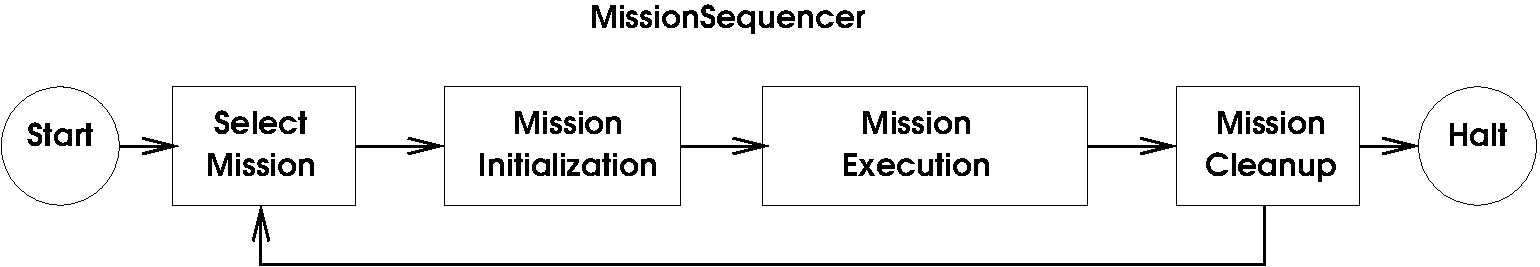
\includegraphics[width=\textwidth]{phases.pdf}
  \caption{A diagram showing the phases of SCJ mission execution}
  \label{phases-diagram}
\end{figure}

The first phase is initialisation, which consists of setting up the
schedulable objects controlled by the mission and creating any data
structures required for the mission.
Then the mission is executed by starting each of the schedulable
objects in the mission and waiting for a request to terminate the
mission.
When the mission is requested to terminate, each of the schedulable
objects in the mission is terminated and the mission's memory is
cleared.

The schedulable objects within a mission are asynchronous event
handlers that are released either periodically, at set intervals of
time, aperiodically, in response to a release request, or once at a
specific point in time (though handlers that are released once can
have a new release time set, allowing them to be released again).
At level 2 real-time threads are also allowed, which run continuously
from when they start until they finish, unless they are suspended or
interrupted by another schedulable object.

Each schedulable object has a priority and the highest priority object
that is eligible to run at each point in time is the object that runs.
This allows for simpler reasoning about order of execution and allows
for more urgent tasks to preempt less urgent tasks.

SCJ allows for assigning schedulable objects to ``scheduling
allocation domains'', where each domain consists of one or more
processors.
At Level 1, each scheduling allocation domain is restricted to a
single processor.
Hence, in scheduling terms, the system is fully partitioned.
This allows for mature single processor schedulability analysis to be
applied to each domain (although the calculation of the blocking times
when accessing global synchronised methods are different than they
would be on a single processor system due to the potential for remote
blocking~\cite{davis2011}).

SCJ deals with memory in terms of memory areas, which are Java objects
that provide an interface to blocks of physical memory called backing
stores.
Memory allocations in SCJ are performed in the backing store of the
memory area designated as the allocation context.
Each schedulable object has a memory area associated with it that is
used as the allocation context during a release of that object, and is
cleared after each release.
Each mission also has a mission memory area that can be used as an
allocation context by the schedulable objects of that mission, to
provide space for objects that need to persist for the duration of the
mission or to be shared between the schedulable objects.
The amount of memory required for the mission memory must be computed
ahead of time and specified by the programmer as part of writing the
mission, though there has been some work on automated computation of
worst case memory use for SCJ programs~\cite{andersen2013}.
There is also an immortal memory area where objects can be allocated
if needed for the entire running of the program (they are never
freed).
SCJ places restrictions on which objects an object may point to, so as
to avoid dangling pointers from being created.
Some examples of valid and invalid object references for some
asynchronous event handlers are shown in
Figure~\ref{stacks-areas-diagram}.

\begin{figure}[ht]
  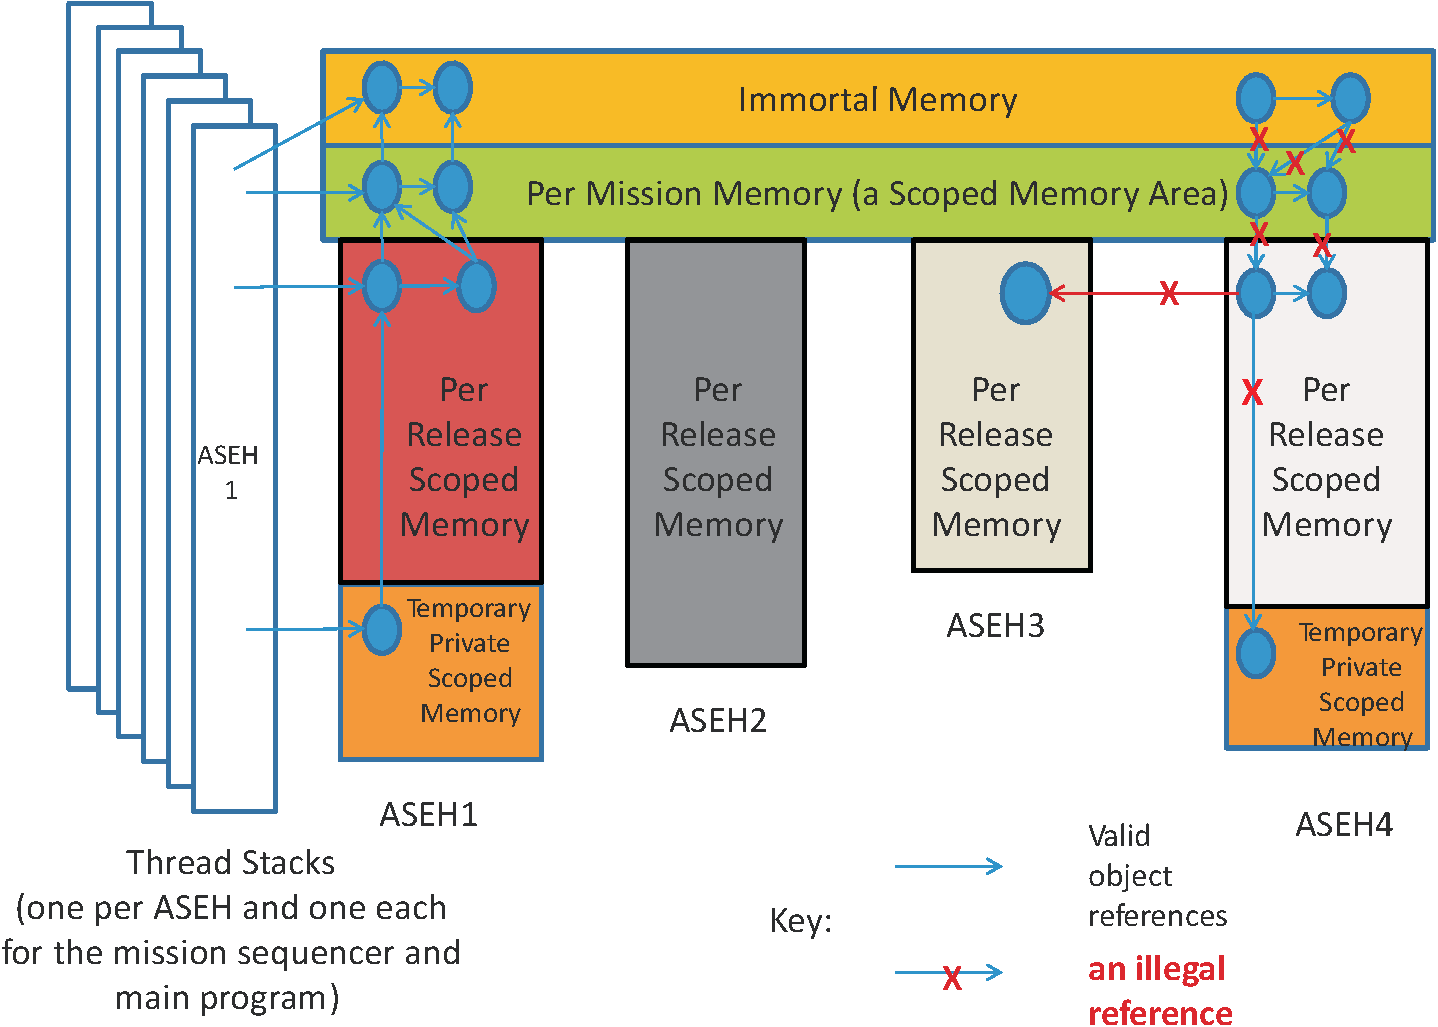
\includegraphics[width=\textwidth]{Stacks-Areas.pdf}
  \caption{An example of the layout of memory areas for four
    asynchronous event handlers (ASEHs), showing possible valid and
    invalid references between them}
  \label{stacks-areas-diagram}
\end{figure}

This system of memory areas makes it easy to predict when memory is
freed.
It is not supported by standard JVMs as they do not provide memory
outside of the heap for allocation and lack a notion of allocation
context.
The SCJ memory manager also needs to provide a means of accessing raw
memory for the purposes of device access, which is mediated by
accessor objects provided by the SCJ API.
As this API was stabilised at a later stage in the development of the
SCJ specification than its other features, we have not had opportunity
to include it in this work.
It can, however, be seen that any system of raw memory access is not
supported by most standard JVMs.

Moreover, dynamic class loading is not allowed in SCJ; all classes
used by the program must be loaded when the program starts.
This is because dynamic class loading may introduce time overheads
that are hard to predict and additional code paths that complicate
certification.
Finally, SCJ also disallows object finalisers as it is not always easy
to predict when they are run.

\section{Virtual Machines for Safety-Critical Java}
\label{virtual-machines-section}

% one subsection per machine

Because of the novel features of SCJ, briefly described in the
previous section, a specialised virtual machine that provides support
for allocation in memory areas and preemptive scheduling is required
for SCJ.
Although SCJ is a relatively recent development there have been
various virtual machines created for SCJ or variations of SCJ,
including icecap HVM~\cite{sondergaard2012}, Fiji VM~\cite{pizlo2009},
OVM~\cite{armbruster2007}, HVM\textsubscript{TP}~\cite{luckow2014} and
PERC Pico~\cite{atego2015, richard2010}.
These are each described in the following subsections.

\subsection{icecap HVM and
  \texorpdfstring{HVM\textsubscript{TP}}{HVMTP}}


The icecap hardware-near virtual machine (HVM) was created as part of
the Certifiable Java for Embedded Systems Project~\cite{schoeberl2014}
and provides an open-source implementation of SCJ targeted at embedded
systems.
The approach taken by the HVM is one of precompiling Java bytecode to
C in order to allow for faster running programs with fewer memory
resources.
It includes an implementation of the SCJ libraries that covers most of
SCJ level 2, originally supporting only single processor programs but
with multiprocessor support added later~\cite{zhao2015}.
This implementation, however, cannot be easily decoupled from the
virtual machine itself.

The icecap HVM also provides a lightweight Java bytecode interpreter
and allows for interpreted code to be mixed with compiled code.
The reason for this is that the bytecode together with the interpreter
can often be smaller than the compiled code, though there is a
tradeoff for speed.
HVM\textsubscript{TP} is a modification of the icecap HVM's bytecode
interpreter to improve time predictability and ensure that bytecode
instructions are executed in constant time, which is important for
ensuring real-time properties of the system hold.

\subsection{Fiji VM}

Fiji VM is a proprietary Java implementation designed to run on
real-time embedded systems.
Similarly to the icecap HVM, Fiji VM uses the strategy of compiling to
C in order to improve performance.
However, Fiji VM is not specifically targeted at SCJ and works with a
range of libraries, including SCJ, RTSJ and the standard Java
libraries.
Fiji VM does have the advantage of high portability and multiprocessor
support, which is lacking in some other SCJ virtual machines.

The fact that Fiji VM works with the SCJ libraries and supports the
scoped memory model means it can run SCJ programs.
It does not necessarily support all aspects of SCJ properly though.

\subsection{OVM}

OVM was created at Purdue University as part of the PCES
project~\cite{baker2006}, to provide a virtual machine that can
execute real-time Java programs with a high level of performance on
embedded systems.
Similar to Fiji VM and icecap HVM, OVM follows the principle of
precompiling code for performance reasons, but translates Java to C++
instead of bytecode to C.

OVM also differs from the icecap HVM and Fiji VM in that it predates
SCJ.
It is written to implement the RTSJ, though it can still support SCJ
programs; indeed, an SCJ implementation for OVM was later
created~\cite{plsek2010}.
However, OVM does not appear to have kept up with more recent changes
to the draft SCJ standard.
OVM is, unlike Fiji VM and the icecap HVM, single processor.

\subsection{PERC Pico}

PERC Pico is a product of Atego based on early ideas for SCJ, but uses
its own system of Java metadata annotations to ensure the safety of
scoped memory.
This systems of annotations provides additional information about how
memory is used so that it can be checked.
Similarly to other SCJ virtual machines, PERC Pico allows for
precompilation of Java code but targets executable machine code rather
than an intermediate programming language.
The metadata annotations are used to guide the compiler to produce
code that uses the correct scoped memory.
PERC Pico does not support the current SCJ standard, though it has
been suggested that it could be modified to do so~\cite{nilsen2011}.

To summarise, as far as we are aware there is one publicly available
virtual machine that has kept up with the developing SCJ
specification, the icecap HVM.
This is and, typically, virtual machines for SCJ will be, designed to
be very small and fast so as to be able to run on embedded systems.

As can be seen from the preceding discussion, a common technique to
run Java programs on embedded systems is to precompile them to native
code.
This means compiler correctness techniques must be considered in
verification of such a virtual machine; these techniques are discussed
in the next section.

\section{Compiler Correctness}
\label{compiler-correctness-section}

Due to the importance of compiler correctness, there has been much
research over the years in this area.
Most of the work done follows a similar approach, which we term
the commuting-diagram approach as it is based on showing that a
particular diagram commutes.
We discuss the commuting-diagram approach in
Section~\ref{commuting-diagram-subsection}.

An alternative approach to compiler verification is the algebraic
approach developed in the early 90s.
It is based on the concepts of refinement calculi designed for
deriving software from specifications of behaviour.
We explain the algebraic approach in
Section~\ref{algebraic-approach-subsection} and discuss how it differs
from the commuting-diagram approach.

We finish in Section~\ref{java-compiler-correctness-subsection} by
reviewing some of the literature on correctness of compilers for
Java-like languages.
We explain how the techniques of compiler correctness have been
applied in the case of Java and compare the different approaches.

\subsection{Commuting-diagram Approach}
\label{commuting-diagram-subsection}

Much of the work on compiler correctness can be seen as following the
approach identified by Lockwood Morris~\cite{morris1973}, and later
refined by Thatcher, Wagner and Wright~\cite{thatcher1979}.
The approach is essentially that a compiler correctness proof is a
proof that the diagram shown in Figure~\ref{commuting-diagram}
commutes, that is, $\gamma \circ \psi = \phi \circ \epsilon$.

\begin{figure}[ht]
  \begin{center}
    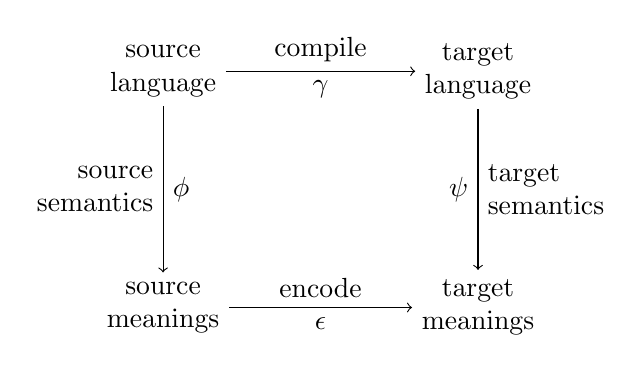
\begin{tikzpicture}
      \node[align=center] (S) at (0cm,3cm) {source\\language};
      \node[align=center] (T) at (4cm,3cm) {target\\language};
      \node[align=center] (M) at (0cm,0cm) {source\\meanings};
      \node[align=center] (U) at (4cm,0cm) {target\\meanings};
      
      \path (S) edge[->] node[align=center, above] {compile}
      node[align=center, below] {$\gamma$} (T); \path (S) edge[->]
      node[align=right, left] {source\\semantics}
      node[align=center,right] {$\phi$} (M); \path (T) edge[->]
      node[align=left, right] {target\\semantics} node[align=center,
      left] {$\psi$} (U); \path (M) edge[->] node[align=center, above]
      {encode} node[align=center, below] {$\epsilon$} (U);
    \end{tikzpicture}
  \end{center}
  \caption{The commuting diagram used in the traditional approach to
    compiler verification}
  \label{commuting-diagram}
\end{figure}

Lockwood Morris had the corners of the diagram as algebras, rather
than merely sets, with the functions between them being homomorphisms
in order to add additional structure to the proof.
This differs from the approach of some earlier works, particularly the
earliest work by McCarthy and Painter~\cite{mccarthy1967}, and instead
follows work such as that of Burstall and Landin~\cite{burstall1969}.

McCarthy and Painter's work featured a simple expression language with
addition, natural numbers and variables.
This was compiled to a simple 4-instruction single-register machine.
The arrows of the diagram were simple functions, rather than
homomorphisms, and the proof was performed using induction over the
source language.
This work laid the foundation for the study of compiler correctness.

Burstall and Landin showed correctness of a compiler for the same
source and target languages as McCarthy and Painter; they used a more
algebraic approach that better matches what Lockwood Morris later
suggested.
Burstall and Landin's approach involved representing the source and
target languages, and their meanings, as algebras, with the
compilation functions as homomorphisms.
They targeted several intermediate machines in the proof of
correctness.
Viewing the languages as algebras allows for simpler proofs as some of
the arrows of the commuting diagram can be wholly or partially derived
from the algebraic structure.
It was this goal of simplifying the proofs that led Lockwood Morris to
advocate the use of algebras and homomorphisms.

The overall goal of pursuing formal proofs of compiler correctness, as
proposed by McCarthy and Painter~\cite{mccarthy1967}, is to allow
machine-checked proofs of program correctness.
There has been work in that area, the earliest of which was that by
Milner and Weyhrauch~\cite{milner1972} who showed the correctness of
an ALGOL-like language.
The proof of correctness was partially mechanised in the LCF theorem
prover~\cite{milner1972a} and the authors were of the opinion that the
proof was feasible and could be completed relatively easily.
A point to note is that Milner and Weyhrauch acknowledged the need for
some way of structuring the proof in order to make it amenable to
machine-checking.
This gives further support to the algebraic commuting-diagram approach
advocated by Lockwood Morris.
Indeed, Milner and Weyhrauch explicitly followed that approach as they
were in discussions with Lockwood Morris.

One advantage to making proofs easily machine-checkable, apart from
the added certainty that the proof is correct, is that working
compilers can be created from the machine-checked proofs.
Code generation facilities are available with many theorem provers
such as those of Isabelle/HOL~\cite{haftmann2007} and
Coq~\cite{letouzey2003, letouzey2008}.
The fact that the commuting-diagram approach involves treating the
compilation as a function between algebras representing the source and
target languages fits well with this idea.
In this case, there is then a function defined in the mechanised logic
for the purposes of conducting proofs about it that can be readily
extracted to executable code.

The commuting-diagram approach has been followed in much of the
literature through the years, though not always with the algebraic
methods recommended by Lockwood Morris.
The basic structure of the commuting diagram is a fairly natural
approach to take, as seen by work such as that of the ProCoS
project~\cite{buth1992}.

Another piece of work that follows the commuting-diagram approach is
that of Polak~\cite{polak1981}, who states that he is more interested
in verification of a ``real'' compiler rather than ``abstract code
generating algorithms'', and shows the correctness of a compiler for a
Pascal-like language.
This work focuses much more on pragmatic applications of the
commuting-diagram approach, leaving behind the algebraic ideas of
earlier papers.
It sets a precedent for a simpler verification approach based on
considering the functions in the commuting diagram.

The commuting-diagram approach has also been used in recent work, some of the
most successful of which is that of CompCert~\cite{leroy2009a,
  leroy2009b, leroy2012}.
This is a project to create a fully verified realistic compiler for a
subset of C, using the theorem prover Coq~\cite{coq2004}.

There is also recent variation of the commuting-diagram approach, 
based on an operational semantics of the source
language~\cite{bahr2015}.
In this work, the operational semantics of the source language and
a way of relating the source and target semantics are used to derive a
different operational semantics of the source language acting on the
state of the target machine.
The semantics of the target language are then identified as part of
that operational semantics and it is transformed to extract a
compilation function.
This approach may be viewed as variant of the commuting-diagram
approach in which the compilation function is derived from the source
and target semantics and the relationship between them, rather than
being verified by those elements of the commuting diagram.

\subsection{Algebraic Approach}
\label{algebraic-approach-subsection}

The second main approach to showing correctness of compilers is the
algebraic approach proposed by Hoare in 1991~\cite{hoare1991}, and
further developed by Sampaio~\cite{hoare1993, sampaio1993,
  sampaio1997}.
We note that the algebraic approach discussed in this section is
largely unrelated to the algebraic commuting-diagram approaches
mentioned in the previous section.

The algebraic approach to compilation derives from the concepts of
algebraic reasoning about programs and program refinement.
These concepts come from the idea, proposed by Hoare in
1984~\cite{hoare1984}, that programs can be thought of as predicates
and so the laws of predicate logic can be used to construct laws for
reasoning about programs~\cite{hoare1987}.
As an example of such a law for reasoning about programs, we present
below associativity of sequential composition,
Equation~\eqref{seq-comp-assoc}, and left and right unit of sequential
composition, namely, the program $\Skip$ that does nothing,
Equation~\eqref{skip-comp-identity}.
\begin{equation}
  \label{seq-comp-assoc}
  P;(Q;R) = (P;Q);R
\end{equation}
\begin{equation}
  \label{skip-comp-identity}
  P;\Skip = \Skip;P = P
\end{equation}

The notion of refinement is central to the algebraic approach to
compilation.
Refinement calculi have been developed, independently, by
Back~\cite{back1981}, Morris~\cite{morris1987} and
Morgan~\cite{morgan1990}, following from earlier concepts of program
transformation~\cite{bauer1976, balzer1976, standish1976, arsac1979}.
The basic idea is that there is a relation between programs that
captures the idea of one program being ``at least as good as'' another
or, to put it more precisely, at least as deterministic as another.
Languages and laws for reasoning about programs with this notion of
refinement can then be used to develop programs from specifications.
This means that certain aspects of a system can have a
nondeterministic specification and several different implementations
can refine that specification.

In using refinement to show the correctness of a compiler, the laws of
the specification language can be used to prove compilation refinement
laws.
These compilation laws can be used to transform the source programs
into some normal form that represents an interpreter for the target
language running the target code.
In other words, the code output by the compiler, when executed by on
the target machine, must be a refinement of the source program.
The compilation laws can be used to prove this refinement and at the
same time generate the target code.

As an example, consider the following refinement in which a simple
program that performs some arithmetic and stores the results into
variables is refined by a normal form representing the target machine
and code.
The symbol $\circrefines$ represents the refinement relation here.
\begin{equation}
  \circvar x, y, z \circspot x := (x + 5) \times (y + z) ; z := z + 1
  \circrefines
  \begin{aligned}
    &\circvar A, P, M \circspot P := 1; \circdo \\
    &\quad            P=1  \then A,    P := M[2],          2 \\
    &\quad \extchoice P=2  \then A,    P := A + M[3],      3 \\
    &\quad \extchoice P=3  \then M[4], P := A,             4 \\
    &\quad \extchoice P=4  \then A,    P := M[1],          5 \\
    &\quad \extchoice P=5  \then A,    P := A + 5,         6 \\
    &\quad \extchoice P=6  \then A,    P := A \times M[4], 7 \\
    &\quad \extchoice P=7  \then M[1], P := A,             8 \\
    &\quad \extchoice P=8  \then A,    P := M[3],          9 \\
    &\quad \extchoice P=9  \then A,    P := A + 1,         10 \\
    &\quad \extchoice P=10 \then M[3] := A,                11 \\
    &\circod ; \{ P = 11 \}
  \end{aligned}
\end{equation}
The normal form represents the behaviour of an interpreter for the
target code running in a target machine whose structure is defined
by the variables A, P, and M.
The variable $A$ represents a general-purpose register of the target
machine, $P$ represents the program counter of the target machine, and
$M$ is an array representing the memory of the target machine.
The normal form consists of a program that initialises $P$ to 1 and
then enters a loop in which the operation performed on each iteration
is dependent on the value of $P$.
The loop is exited when $P$ is set to a value for which there is no
operation and it is asserted that $P$ will be equal to 11 at the end
of the program.
Each of the statements of the source program corresponds to several
operations in the normal form as complex expressions are broken down
into simpler expressions that can be handled by instructions of the
target machine.

The compilation proceeds by first applying rules to simplify the
assignment statements.
The register $A$ is introduced at this stage by splitting assignments
of expressions to variables into two assignments that transfer the
values to and from $A$.
In this way, the assignments are transformed for the target machine
that only has instructions involving registers.
Particularly complex expressions such as $(x + 5) \times (y + z)$ are
handled by storing intermediate results in temporary variables.
In this case the result of the expression $y + z$ is placed in a
temporary variable when $P = 3$.
The variables used in the source program and introduced compilation
are later replaced with locations in the memory array $M$ in a data
refinement step.
This causes the variables $x$, $y$ and $z$ to be replaced with $M[1]$,
$M[2]$ and $M[3]$ respectively.
The temporary variable introduced to store the result of $y + z$ is
similarly replaced with $M[4]$.

Each of the assignment statements is then refined by a normal form
with an explicit program counter $P$, that is incremented as part of
the assignment operation.
These normal forms are then combined together by the refinement rule
for sequential composition to create the normal form of the full
program.
The update of the program counter in this program is quite simple but
more complex updates would occur for conditionals or loops.

The power of the algebraic approach is that the compilation of
individual elements of the source language can be specified and proved
separately in different refinement laws.
The compilation can also be split into stages, with a set of
refinement laws for each stage to modularise the compilation.
The separate refinement laws can then be combined to form a
compilation strategy.

The first major work done using the algebraic approach was that of
Sampaio~\cite{sampaio1993}, who used it to specify a correct compiler
for a simple language that, nonetheless, covers all the constructs
available in most programming languages.
The target machine Sampaio used was a simple single-register machine
that bears similarity to most real processor architectures.
He mechanised the compiler in the OBJ3 term rewriting
system~\cite{goguen1988}, showing that working compilers can be easily
created from specifications using the algebraic approach.
However, the algebraic laws Sampaio used to prove correctness of the
compiler were taken as axioms.
Sampaio notes that they could be easily proved given a semantics for
the reasoning language.

Though there has not been much work done using the algebraic approach,
we single out the work of Perna~\cite{perna2010, perna2011}, showing
correctness of a compiler for a hardware description language.
The compilation takes high-level descriptions of hardware written in
Handel-C and transforms them into systems of basic hardware components
connected by wires.
The algebraic approach works well here as the target language is a
subset of the source language, albeit in a different form.
Perna was able to handle features not covered by most other works on
hardware compilation, such as parallelism with shared variables.
Also, whereas Sampaio took the basic algebraic laws as axioms, Perna
proved the laws from a semantics given using the Unifying Theories of
Programming (UTP) model~\cite{hoare1998}.
There has also been work on the correctness of Java compilers using
the algebraic approach.
This is considered in the next section, where we consider compiler
correctness for Java-like languages.

\subsection{Correctness of Java Compilers}
\label{java-compiler-correctness-subsection}

The popularity of Java has meant that there has been plenty of work on
formalising Java and the JVM~\cite{hartel2001}, but there have been
relatively few works on formally verified compilers for Java-like
languages.
However, the work that has been done uses both of the two main
approaches and covers most of the features of Java.

Some of the earliest and most thorough work is that by S\"{a}rk,
Schmid and B\"{o}rger~\cite{stark2001}, who formalise most of Java and
the JVM before specifying and showing the correctness of a compiler
for Java.
The approach taken by them uses Abstract State Machines (ASMs) to
specify the source and target languages.
The ASMs give an operational semantics to Java and the JVM, describing
how each construct affects the running of the program.
The languages are each specified by multiple ASMs, beginning with an
imperative core, then adding classes, objects, exceptions and,
finally, threads.

Although this approach is called the ASM approach, it becomes clear
from the definition of compiler correctness given in terms of a
mapping between ASMs that this work ultimately follows the
commuting-diagram approach.
This work leaves parts of the proof incomplete (in particular,
compilation of threads is not addressed) and applies to an old version
of Java.
This is, nevertheless, an admirable attempt at producing a verified
Java compiler.

Work has also been done by Duran following the algebraic
approach~\cite{duran2005, duran2010}.
Duran's work specifies a compiler for a language called Refinement
Object-Oriented Language (ROOL)~\cite{borba2000}, which was created
for reasoning about object-oriented languages and bears much
similarity to Java.
ROOL features constructs for specifying and reasoning about programs
as well as object-oriented programming language constructs.
This means that the there are algebraic laws for ROOL, from which the
rewrite rules that form the basis of the algebraic approach can be
proved.
Duran's work adds further phases to Sampaio's compilation strategy in
order to deal with the object-oriented features, but does not consider
some other aspects of Java such as exceptions and threads.
Duran notes that other work has addressed some of those issues.

While the two works already discussed were not machine checked, there
have also been compiler correctness proofs for Java-like languages in
the Isabelle/HOL proof assistant.
The first of these was by Strecker~\cite{strecker2002}, showing
correctness of a compiler for a subset of Java called $\mu$Java, which
already had a formalisation of its semantics in
Isabelle/HOL~\cite{nipkow2000}.
This work was followed by Klein and Nipkow's work on a compiler for a
slightly larger subset of Java called Jinja~\cite{klein2006}, which
added exception handling.
Finally, Lochbihler~\cite{lochbihler2010} added threads to Jinja and
showed correctness of compilation for Java concurrency.
It is notable that this is the only work on Java compilation that
properly addresses concurrency.
All of these works follow the commuting-diagram approach.

Though some work has been done on correct compilers for Java-like
languages and many virtual machines for SCJ adopt an approach of
compiling to native code, no work has been done on verifying that
compilation to native code.
Therefore, in this thesis, we consider correctness of the compilation
to native code as part of our work on SCJ virtual machines.
We follow the algebraic approach as it gives greater assurance of
correctness, as an additional function mapping source meanings to
target meanings is not required, and a good level of modularity, as
the compilation is split into separately proved rewrite rules.
In order to represent the normal form we require a specification
language and for that purpose use \Circus{}, which is described
in the next section.

\section{\Circus{}}
\label{circus-section}

The \Circus{} specification language~\cite{oliveira2009} is based on
CSP~\cite{roscoe2011}, which is used to specify processes that
communicate over channels, and the Z notation~\cite{woodcock1996},
which is used to specify state and data operations.
A \Circus{} specification is made up of processes that communicate
over channels.
These channels may carry values of a particular type, or may be used
as flags for synchronisation or signalling between processes.
Each process may have state, and is made up of actions that operate on
that state and communicate over channels.

We illustrate the concepts of \Circus{} using as an example the
process for the real-time clock from an early version of our
specification of an SCJ virtual machine.
The specification begins with a declaration of the channels that may
be used in the following processes.
Type declarations written in Z can also be included at the beginning
of a \Circus{} specification.
Here, we define a type $Time$ to be the set of natural numbers and
create a boolean datatype
%
\begin{zed}
  Time == \nat \\
  Bool ::= True | False
\end{zed}
%
We declare channels to represent interactions corresponding to calls
to methods to get the clock's time and precision, and set and clear
alarms.
Channels are also declared to model interactions with the hardware
that accept clock tick interrupts and read the time from the hardware
clock.
%
\begin{circus}
  \circchannel getTime, getPrecision, setAlarm : Time \\
  \circchannel clearAlarm \\
  \circchannel HWtick \\
  \circchannel HWtime : Time
\end{circus}
%
We also specify a constant to represent the clock's precision using a
Z axiomatic definition.
The value of the constant is required to be nonzero, but is otherwise
left unrestricted, so that any nonzero time value is a valid
instantiation.
%
\begin{axdef}
  precision : Time \where precision > 0
\end{axdef}
%
After the channel declarations, we can declare processes that use
them.
Here we declare the $RealtimeClock$ process.
It is a basic process, that is, its state is defined in Z, and its
behaviour using CSP constructs and Z data operations.
%
\begin{circus}
  \circprocess RealtimeClock \circdef \circbegin
\end{circus}
%
In this example, the state records the current time, whether an alarm
is set, and the time of the alarm that may be set.
An invariant specifies that if an alarm is set, then the time of the
alarm must not be in the past.
%
\begin{schema}{RTCState}
  currentTime  : Time \\
  alarmSet     : Bool \\
  currentAlarm : Time
\where
  alarmSet = True \implies \\
  \t1 currentAlarm \geq currentTime
\end{schema}
\begin{circusaction}
  \circstate RTCState
\end{circusaction}
%
The behaviour is described using actions, written in a mixture of Z
and CSP.
The first action is a Z initialisation operation, $Init0$.
Its final state is represented by variables obtained by placing a
prime on the names of the state components.
Here, the initialisation takes as input the initial time, represented
by the variable $initTime?$.
In Z schemas, inputs to operations are distinguished by ending with a
question mark.
Similarly, outputs are marked with an exclamation mark.
The current time is defined to be equal to the initial time and no
alarm is initially set.
The initial time of the alarm is arbitrary, that is,
nondeterministically chosen from elements of its type, since the
initialisation imposes no restrictions on it.
%
\begin{schema}{Init0}
  RTCState~' \\
  initTime? : Time
\where 
  currentTime' = initTime? \\
  alarmSet' = False
\end{schema}
%
The action $Init$, defined below, uses a CSP prefixing to specify an
input communication before the initialisation operation $Init0$.
The initial time of the clock is read from the hardware clock and then
the initialisation specified by the Z schema is performed.
%
\begin{circusaction}
  Init \circdef HWtime?initTime \then Init0
\end{circusaction}
%
The action that returns the current time simply uses CSP to output the
current time from the state over the $getTime$ channel.
The action ends with the special action $\Skip$, which indicates the
end of an action.
%
\begin{circusaction}
  GetTime \circdef getTime!currentTime \then \Skip
\end{circusaction}
%
Setting a new alarm is a more complex operation that involves Z
schemas that specify two different scenarios in which this operation
may be used.
In the first case, the new alarm is not in the past.
The symbol $\Delta$ denotes a change of state.
The operation stores the time of the new alarm and sets a flag to
indicate an alarm is set in this case.
%
\begin{schema}{SetAlarm0}
  \Delta RTCState \\
  newAlarm? : Time
\where
  newAlarm? \geq currentTime \\
  currentAlarm' = newAlarm?{} \\
  alarmSet' = True \\
  currentTime' = currentTime
\end{schema}
%
In the second case, the new alarm is in the past and so the alarm is
not set (we have omitted the error reporting for the sake of
simplicity).
The symbol $\Xi$ denotes that the state remains the same.
%
\begin{schema}{SetAlarm1}
  \Xi RTCState \\
  newAlarm? : Time
\where
  newAlarm? < currentTime
\end{schema}
%
The two Z schemas are combined using a logical disjunction, allowing
either to specify the behaviour when a request to set the alarm takes
place.
%
\begin{circusaction}
  SetAlarm \circdef setAlarm?newAlarm \then \lschexpract SetAlarm0 \lor SetAlarm1 \rschexpract
\end{circusaction}
%
In addition to Z and CSP constructs, \Circus{} also has other
constructs more familiar to programmers, such as if statements and do
loops.
One of these constructs, the assignment operator, is used in the
action that clears the current alarm to update part of the state
without requiring a Z schema.
The alarm is cleared by simply setting $alarmSet$ to $False$, without
updating any other state variables.
%
\begin{circusaction}
  ClearAlarm \circdef clearAlarm \then alarmSet := False
\end{circusaction}
%
Each of the actions the process can perform are joined together with
the CSP external choice operator, which chooses an action to take
based on the channel communications that the environment is willing to
perform.
This includes the actions above, as well as some other actions that
have been omitted here.
The choice is repeated in a loop.
%
\begin{circusaction}
  Loop \circdef \left( GetTime \extchoice SetAlarm \extchoice
    ClearAlarm
    \extchoice \cdots \right) \\
  \t1 \circseq Loop
\end{circusaction}
%
The \Circus{} process then ends with the main action that specifies
the overall behaviour of the process.
Here, the process simply performs the initialisation and then enters
the loop.
%
\begin{circusaction}
  \circspot Init \circseq Loop
\end{circusaction}
\begin{circus}
  \circend
\end{circus}

In addition to the constructs presented here \Circus{} also contains
operators for composing processes in parallel, with or without
synchronisation on channels.
These operators are used both to specify actual parallelism and to
represent composition of requirements.
In this way several \Circus{} specifications of individual components
can be combined to form a specification of the entire system.

A detailed account of \Circus{} can be found in~\cite{oliveira2009}.
Table~\ref{circus-operators-table} summarises the \Circus{} constructs
used in this thesis.

\begin{table}
  \centering
  \begin{tabular}{p{11.3cm}l}
    \hline
    Construct & \Circus{} notation \\
    \hline
    Termination & $\Skip$ \\
    Divergence (abortion) & $\Chaos$ \\
    Assignment of expression $e$ to variable $x$ & $x := e$ \\
    Prefixing of signal on channel $c$ to action $A$ & $c \then A$ \\
    Prefixing of output on channel $c$ of expression $e$ to action $A$ & $c!e \then A$ \\
    Prefixing of input on channel $c$ of variable $x$ to action $A$ & $c?x \then A$ \\
    Variable block with variable $x$, of type $T$, and action $A$ & $\circvar x : T \circspot A$ \\
    Value parameter block with parameter $x$, of type $T$, and action $A$ & $\circval x : T \circspot A$ \\
    Result parameter block with parameter $x$, of type $T$, and action $A$ & $\circres x : T \circspot A$ \\
    Instantiation of parameterised action $A$ with expression $e$ & $A(e)$ \\
    Guarding of $A$ with predicate $g$ & $\lcircguard g \rcircguard \circguard A$ \\
    Sequential composition of actions $A$ and $B$ & $A \circseq B$ \\
    External choice of actions $A$ and $B$ & $A \extchoice B$ \\
    Conditional choice of actions $A$ and $B$, with conditions $g$ and $h$ & $\circif g \circthen A \circelse h \circthen B \circfi$ \\
    Parallel interleaving of processes $P$ and $Q$ & $P \interleave Q$ \\
    Recursion with body given by action function $F$ & $\circmu X \circspot F(X)$ \\
    Parallel composition of processes $P$ and $Q$, synchronising on the \endgraf \hspace{1cm} intersection of channel sets $cs1$ and $cs2$ & $P _{cs1}\!\!\parallel_{cs2} Q$ \\
    Parallel composition of processes $P$ and $Q$, synchronising on the \endgraf \hspace{1cm} channel set $cs$ & $P \lpar cs \rpar Q$ \\
    Hiding of channel set $cs$ in process $P$ & $P \circhide cs$ \\
    \hline
  \end{tabular}
  \caption{Summary of \Circus{} notation}
  \label{circus-operators-table}
\end{table}

% for the thesis add a more comprehensive description of Circus with a
% description of process operators and tables of operator descriptions

\section{Final Considerations}
\label{final-considerations-section}

% summarise the problem and how to solve it

We have seen that Java is increasingly being considered as a language
for safety-critical embedded systems and that the modifications to
Java required to make it suitable for such systems require a
specialised virtual machine.
The developing Safety-Critical Java specification has several
differences from standard Java, particularly in the areas of
scheduling and memory management, that make standard JVMs unsuitable
for running SCJ programs.
We have considered several virtual machines that have been developed
for running SCJ programs and noted that none of them has been formally
verified and that most of them adopt an approach of precompiling
programs to native code.

With that in mind, we have considered the techniques used to verify
the correctness of compilers and found that there are two main
approaches: the commuting-diagram approach and the algebraic approach.
In the commuting-diagram approach the source semantics, target
semantics, compilation function, and a function mapping the source
meanings to the target meanings, are shown to commute.
This approach is popular and has had much research done on it but
relies on the definition of the function from the source meanings to
the target meanings.

The algebraic approach defines the source and target languages within
the same specification language, which is additionally equipped with a
refinement relation between programs.
Laws of the specification language are then used to prove refinement
rules that are applied according to some compilation strategy.
The algebraic approach has the advantage that it does not require the
additional function that is required in the commuting-diagram
approach, since the source and target languages are defined in terms
of the same specification language.
The algebraic approach also permits a modular approach to proof and
allows for the compiler to be easily implemented by application of the
refinement rules using a term rewriting system.

Given the considerations above, we have decided to adopt the algebraic
approach when specifying the compilation to native code employed by
many SCJ virtual machines.
This means that a specification language is required in which to
define the source and target languages, as well as for the purposes of
specifying other aspects of the virtual machine.
We have chosen \Circus{} as the specification language as it contains
a wide variety of constructs that allow for specification of both data
and behaviour, has a well defined semantics with many laws already
proved, and has been used for previous work on the specification of
SCJ programs.
\Circus{} also has some existing mechanisation and tool support, which
can help give greater assurance of the correctness of specifications.

\chapter{Safety-Critical Java Virtual Machine Services}
\label{scjvm-services-chapter}

In order to reason about a Safety-Critical Java virtual machine
(SCJVM), we first require an identification of the the requirements of
an SCJVM and a formal model of those requirements.
For the purposes of our model, we consider an SCJVM to have the
components illustrated in Figure~\ref{scjvm-services-fig}.
An SCJVM is divided into two main parts:~the core execution
environment and the SCJVM services that may make use of the services
of an underlying operating system or hardware abstraction layer.

\begin{figure}[ht]
  \centering
  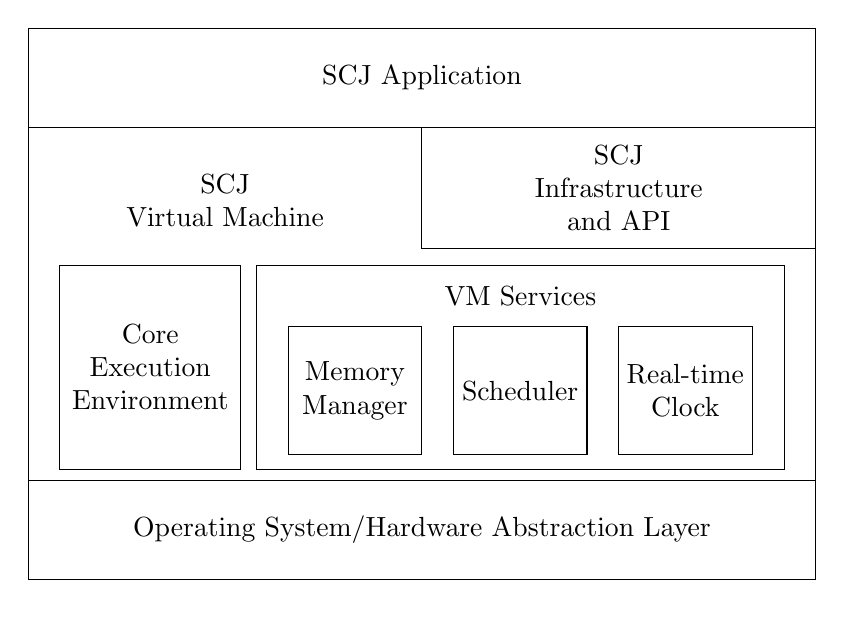
\begin{tikzpicture}

    \coordinate (width)  at (10cm,0cm);
    \coordinate (height) at (0cm,7cm);

    \path (0,0) -- (height)
    coordinate[pos=0.18] (OS boundary)
    coordinate[pos=0.20] (VM part bottom)
    coordinate[pos=0.57] (VM part top)
    coordinate[pos=0.60] (API boundary)
    coordinate[pos=0.82] (App boundary);
    
    \path (VM part bottom) -- (VM part top)
    coordinate[pos=0.7] (VM Service top);

    \path (VM part bottom) -- (VM part top)
    coordinate[pos=0.85] (VM Services ypos);

    \path (0,0) -- (width)
    coordinate[pos=0.04] (CEE left)
    coordinate[pos=0.27] (CEE right)
    coordinate[pos=0.29] (VM Services left)
    coordinate[pos=0.96] (VM Services right)
    coordinate[pos=0.17] (VM Service width)
    coordinate[pos=0.04] (VM Service sep);

    \path (VM Services left) -- (VM Services right)
    coordinate[pos=0.5] (VM Services xpos);

    \path (0,0) to node[pos=0.5] (mid) {} (width);
    \path (0,0) to node[pos=0.25] (quart) {} (width);

    \draw (0,0) rectangle (width |- height);

    \draw (OS boundary) -- ++(width);
    \path (0,0) rectangle node[pos=0.5] (OS) {} (width |- OS boundary);
    \draw (mid |- API boundary) rectangle node[pos=0.5] (API) {} (width |- App boundary);
    \draw (App boundary) -- ++(width);
    \path (App boundary) rectangle node[pos=0.5] (App) {} (width |- height);

    \path (quart |- API boundary) rectangle node[pos=0.4] (SCJVM) {} (quart |- App boundary);
    \draw (CEE left |- VM part bottom) rectangle node[pos=0.5] (CEE) {} (CEE right |- VM part top);
    \draw (VM Services left |- VM part bottom) rectangle (VM Services right |- VM part top);
    \coordinate (VM Services) at (VM Services xpos |- VM Services ypos);

    \node[align=center] at (App)   {SCJ Application};
    \node[align=center] at (API)   {SCJ\\Infrastructure\\and API};
    \node[align=center] at (SCJVM) {SCJ\\Virtual Machine};
    \node[align=center] at (CEE)   {Core\\Execution\\Environment};
    \node[align=center] at (OS)    {Operating System/Hardware Abstraction Layer};
    
    \foreach \x in {1,...,3}
    \pgfmathsetmacro{\a}{0.333*(\x - 1)}
    \pgfmathsetmacro{\b}{0.333*\x}
    \path ($(VM Services left) + (VM part bottom)!0.07!(VM part top)$) -- 
    node[pos=\a] (VM Service \x start) {}
    node[pos=\b] (VM Service \x end) {}
    ($(VM Services right) + (VM part bottom)!0.07!(VM part top) - (VM Service sep)$);

    \foreach \x in {1,...,3} 
    \draw ($(VM Service \x start) + (VM Service sep)$)
    rectangle node[pos=0.5] (VM Service \x) {}
    (VM Service \x end |- VM Service top);

    \node[align=center] at (VM Services)  {VM Services};
    \node[align=center] at (VM Service 1) {Memory\\Manager};
    \node[align=center] at (VM Service 2) {Scheduler};
    \node[align=center] at (VM Service 3) {Real-time\\Clock};
  \end{tikzpicture}
  \caption{A diagram showing the structure of an SCJVM and its
    relation to the SCJ infrastructure and the operating
    system/hardware abstraction layer, focusing on the SCJVM services}
  \label{scjvm-services-fig}
\end{figure}

The core execution environment manages the execution of Java bytecode,
whether that be via interpretation, just-in-time compilation or
ahead-of-time compilation.
The core execution environment must also manage data that relates to
the execution of bytecode instructions, such as the representation of
classes and objects.

The SCJVM services represent the additional services that must be
offered by an SCJVM in order to support the SCJ infrastructure.
These services may be supplied as standalone services and so do not
need to be handled by the compilation strategy.
We consider the virtual machine services to be divided into three
areas:
\begin{itemize}
\item the memory manager, which manages backing stores for memory areas and
  allocation within them;
\item the scheduler, which manages threads and interrupts, and allows for
  implementation of SCJ event handlers; and
\item the real-time clock, which provides an interface to the system real-time
  clock.
\end{itemize}
Each of these services is used either by the core execution environment or by
the SCJ infrastructure; some of the services also rely on each other.  For
example, the scheduler must update the allocation context in the memory manager
when performing a thread switch.

A model of the core execution environment is presented in
Chapter~\ref{cee-chapter}.
In this chapter, we present the requirements for each area of the
SCJVM services:~the memory manager in
Section~\ref{memory-manager-section}, the scheduler in
Section~\ref{scheduler-section}, and the real-time clock in
Section~\ref{realtime-clock-section}.
The formal model of the SCJVM requirements is presented in
Section~\ref{formal-model-section}.
A complete version of the model can be found in
Appendix~\ref{full-scjvm-services-model}

The memory manager model has been subject to proof using Z/Eves.
The theorems proved about the memory manager can be found in
Appendix~\ref{memory-manager-theorems}, with the Z/Eves proof scripts
in Appendix~\ref{memory-manager-proofs}.
Many additional lemmas about objects in the Z/Eves mathematical
toolkit have been proved in the course of carrying out these proofs.
As these can be of use outside our work, we have included them
separately in Appendix~\ref{additional-lemmas} with their proofs in
Appendix~\ref{additional-lemmas-proofs}.

Part of an earlier version of this model was presented at the 13th
International Workshop on Java Technologies for Real-time and Embedded
Systems~\cite{baxter2015a} with the full earlier version made available
as a technical report~\cite{baxter2015}.

\section{Memory Manager API}
\label{memory-manager-section}

The SCJVM memory manager deals with the raw blocks of memory used as
backing stores for the memory areas of SCJ.
The memory areas themselves are Java objects, and so are dealt with by
the core execution environment and accessed through the SCJ API,
instead of directly via the virtual machine.
This is in line with what is specified in the SCJ standard and also
done for RTSJ.
Backing stores are assumed to have unique identifiers that can be used
to refer to them; these identifiers can be simply pointers to the
physical blocks of memory used for backing stores.

There is initially one backing store, called the root backing store,
which has its size set when the SCJVM starts up to cover all the
memory available for allocation in backing stores.
The root backing store cannot be resized or destroyed, so that there
is always a fixed base for the layout of memory.
The root backing store is used as the backing store for the immortal
memory area.

A backing store may have other backing stores nested within it, so
that a possible memory layout is as shown in Figure~\ref{memory-fig}.
In this example, the backing store of the mission memory is nested
within the root backing store, and the backing stores for the
per-release memory of each schedulable object in a mission is nested
within the mission memory's backing store.

\begin{figure*}[ht]
  \centering
  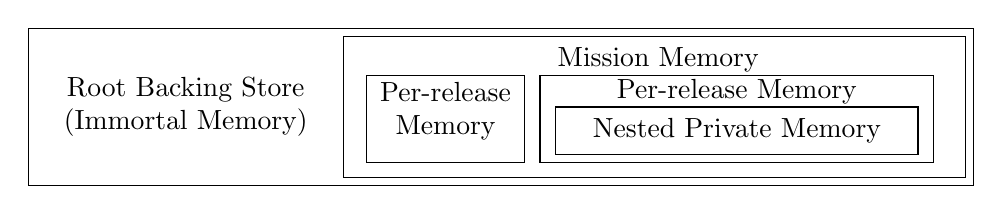
\begin{tikzpicture}
    \draw (0,0) rectangle (12,2); \node[align=center] at (2,1) {Root
      Backing Store\\(Immortal Memory)};
    
    \draw (4,0.1) rectangle (11.9,1.9); \node[align=center] at (8,1.6)
    {Mission Memory};
    
    \draw (4.3,0.3) rectangle (6.3,1.4); \node[align=center] at
    (5.3,0.95) {Per-release\\Memory};
    
    \draw (6.5,0.3) rectangle (11.5,1.4); \node[align=center] at
    (9,1.2) {Per-release Memory};
    
    \draw (6.7,0.4) rectangle (11.3,1); \node[align=center] at (9,0.7)
    {Nested Private Memory};
  \end{tikzpicture}
  \caption{An example memory layout}
  \label{memory-fig}
\end{figure*}

The operations of the memory manager API are summarised in
Table~\ref{memory-manager-table}.
In addition to the inputs and outputs described there, there should
also be some system of reporting erroneous inputs, whether that be
exceptions, global error flags, or particular return values signalling
errors.
The conditions that cause an error to be reported are listed in
Table~\ref{memory-manager-table} as well.

\begin{table*}[ht]
  \centering
  \footnotesize
  \begin{tabular}{|l|p{3.1cm}|p{3.1cm}|p{3.9cm}|}
    Operation & Inputs & Outputs & Error Conditions \\
    \hline
    \texttt{getRootBackingStore} &
    (none) &
    backing store identifier &
    (none)
    \\\texttt{getTotalSize} &
    backing store identifier &
    size in bytes &
    invalid identifier
    \\\texttt{getUsedSize} &
    backing store identifier &
    size in bytes &
    invalid identifier
    \\\texttt{getFreeSize} &
    backing store identifier &
    size in bytes &
    invalid identifier
    \\\texttt{findBackingStore} &
    memory pointer &
    backing store identifier &
    no backing store found
    \\\texttt{allocateMemory} &
    backing store identifier \newline
    size in bytes &
    memory pointer &
    invalid identifier \newline
    insufficient free memory \newline
    no current allocation context
    \\\texttt{makeBackingStore} &
    backing store identifier \newline
    size in bytes & 
    backing store identifier &
    invalid identifier \newline
    insufficient free memory
    \\\texttt{clearBackingStore} &
    backing store identifier &
    (none) &
    invalid identifier \newline
    nested backing store in use
    \\\texttt{resizeBackingStore} &
    backing store identifier \newline
    size in bytes &
    backing store identifier &
    invalid identifier \newline
    backing store in use \newline
    backing store is root \newline
    backing store not empty \newline
    backing store not only child \newline
    insufficient free space \newline
    no space for memory overhead
    \\\texttt{createStack} &
    size in bytes &
    stack identifier &
    insufficient free space
    \\\texttt{destroyStack} &
    stack identifier &
    (none) &
    invalid identifier \newline
    stack space fragmentation
  \end{tabular}
  \caption{The operations of the SCJVM memory manager}
  \label{memory-manager-table}
\end{table*}

The root backing store is always available to the SCJ infrastructure
through the \texttt{get\-Root\-Backing\-Store} operation.
An SCJ program, on the other hand, does not have direct access to the
root backing store except through memory areas provided by the
infrastructure.

It is possible to obtain information about the used and available
space in a given backing store using the operations
\texttt{get\-Total\-Size}, \texttt{get\-Used\-Size}, and
\texttt{get\-Free\-Size}.
This information is made available to SCJ programs through the
interface provided by memory areas defined in the infrastructure.

The backing stored in which a particular memory address lies can also
be queried.  
This information can be obtained by the \texttt{find\-Backing\-Store}
operation and is required by the infrastructure for obtaining the
memory area of a given object.

Allocation within backing stores is possible through the
\texttt{allocate\-Memory} operation, which allocates blocks of memory
within a given backing store.
This operation is provided in order for the core execution environment
to implement the \texttt{new} bytecode instruction and is not directly
available to the program or infrastructure.
Though the memory manager allocates space for objects, there is no
notion of objects in the memory manager since they only exist at the
level of Java code, and so are dealt with by the core execution
environment. 
Dealing solely with blocks of memory in the SCJVM services allows for
objects to be represented in a way appropriate to the structure of the
core execution environment.
Allocations within backing stores must not cause fragmentation, so as
to fulfil real-time predictability requirements.
The operation \texttt{allocate\-Memory} must also zero the memory it
allocates, in order to match the semantics of \texttt{new}.
 
Allocation of backing stores is provided by
\texttt{make\-Backing\-Store}, which is available to the
infrastructure for use when creating new memory areas.
A new backing store is created nested within the specified backing
store.
The infrastructure is responsible for storing the backing store
identifier returned by \texttt{make\-Backing\-Store}.
Backing store allocation must be done in constant time without
fragmentation.

Deallocation of memory in backing stores cannot be done directly as
that could introduce fragmentation and would defeat the scoped-memory
model of SCJ.
Instead, the SCJVM provides for clearing a backing store when the
memory area it serves is no longer in use.
This functionality is provided by the operation
\texttt{clear\-Backing\-Store}, which clears the specified backing
store, deallocating all objects and nested backing stores within it.
It is not necessary to track exactly which objects are deallocated by
this operation as SCJ does not have object finalisers.
The clearing of a backing store includes the clearing of all backing
stores nested within it, whose memories are freed with the rest of the
backing store.
This would create a problem if the parent backing store were cleared
while another thread is using a backing store within it as an
allocation context.
Such a situation should not occur as the backing stores of mission
memory and immortal memory are the only ones that contain backing
stores in use by different threads.
The mission memory is only cleared when all the event handler threads
within the mission have finished and the immortal memory should never
be cleared.
An attempt to clear a backing store with a nested backing store in use
is handled as an error case.

The last operation on backing stores is their resizing.
This is provided for by \texttt{resize\-Backing\-Store} but, as
resizing a backing store presents a lot of difficulties in terms of
fragmentation, there are several restrictions.
In addition to being a valid backing store and there being enough
space in the parent backing store for the resizing to take place, a
backing store to be resized must not be the root backing store, and
must be empty and the only backing store within its parent.
This operation should only be needed for resizing of the mission
memory in between missions and resizing of a nested private memory
when it is reentered.
In both these cases all the needed restrictions hold.
Due to the fact that resizing a backing store can move it and that a
backing store identifier may be a pointer to the backing store, the
identifier may change and so the new identifier is output from this
operation.

These operations on backing stores each take a backing store
identifier as input since the memory manager does not handle
allocation contexts.
Management of allocation contexts is instead left to the core
execution environment, which must pass the appropriate backing store
identifier when using the memory manager services.

The memory manager must also manage stacks, which are placed in a
separate area of memory to the backing stores.
The operations \texttt{create\-Stack} and \texttt{destroy\-Stack}
allow for stacks to be created and destroyed.
The stack space must not be fragmented, which is a requirement that
can be met since stacks for threads are allocated together when a
mission is initialised and destroyed together when the mission ends.
That remains true at level 2 where nested missions are permitted,
since the nested mission's stacks are allocated after the stacks of
its parent mission, and are destroyed before the parent mission ends.
Like backing stores, stacks are referred to by unique identifiers that
may simply be pointers to the space allocated for the stack.

The memory manager must interact with the scheduler to obtain the
current thread when it needs to operate on the current allocation
context.
The next section gives an overview of the scheduler.

\section{Scheduler API}
\label{scheduler-section}

The SCJVM scheduler manages the scheduling of threads, which are
abstract lines of execution, each with its own stack and current
allocation context.
These threads are useful, for example, to implement the event handlers
of SCJ, with each event handler being bound to a single thread.
The operations of the scheduler are summarised in
Table~\ref{scheduler-table}.

\begin{table*}[ht]
  \centering
  \footnotesize
  \begin{tabular}{|l|p{3.2cm}|p{2.3cm}|p{3.6cm}|}
    Operation & Inputs & Outputs & Error Conditions \\
    \hline
    \texttt{getMaxSoftwarePriority} &
    (none) &
    priority level &
    (none)
    \\\texttt{getMinSoftwarePriority} &
    (none) &
    priority level &
    (none)
    \\\texttt{getNormSoftwarePriority} &
    (none) &
    priority level &
    (none)
    \\\texttt{getMaxHardwarePriority} &
    (none) &
    priority level &
    (none)
    \\\texttt{getMinHardwarePriority} &
    (none) &
    priority level &
    (none)
    \\\texttt{getMainThread} &
    (none) &
    thread identifier &
    (none)
    \\\texttt{makeThread} &
    priority level \newline
    class identifier \newline
    method identifier \newline 
    argument list &
    thread identifier &
    (none)
    \\\texttt{startThreads} &
    list of thread and backing store identifiers &
    (none) &
    invalid identifier \newline
    thread already started
    \\\texttt{getCurrentThread} &
    (none) &
    thread identifier &
    (none)
    \\\texttt{destroyThread} &
    thread identifier &
    (none) &
    invalid identifier \newline
    thread not destroyable
    \\\texttt{suspendThread} &
    (none) &
    (none) &
    thread cannot be blocked \newline
    thread holds locks
    \\\texttt{resumeThread} &
    thread identifier &
    (none) &
    invalid identifier \newline
    thread not blocked
    \\\texttt{setPriorityCeiling} &
    pointer to object \newline
    priority level &
    (none) &
    invalid priority
    \\\texttt{takeLock} &
    pointer to object &
    (none) &
    lock in use
    \\\texttt{releaseLock} &
    pointer to object &
    (none) &
    lock not held
    \\\texttt{attachInterruptHandler} &
    interrupt identifier \newline
    backing store identifier \newline
    class identifier \newline
    pointer to object &
    (none) &
    (none)
    \\\texttt{detachInterruptHandler} &
    interrupt identifier &
    (none) &
    (none)
    \\\texttt{getInterruptPriority} &
    interrupt identifier &
    priority level &
    (none)
    \\\texttt{disableInterrupts} &
    (none) &
    (none) &
    (none)
    \\\texttt{enableInterrupts} &
    (none) &
    (none) &
    (none)
    \\\texttt{endInterrupt} &
    (none) &
    (none) &
    not in interrupt
  \end{tabular}
  \caption{The operations of the SCJVM scheduler}
  \label{scheduler-table}
\end{table*}

Each thread is scheduled according to a priority level.
The SCJ standard requires that there be at least 28 priorities and
separates them into hardware and software priorities, with hardware
priorities being higher than software priorities.
The range of priorities that an SCJVM actually supports may vary
between different implementations within these restrictions.
To allow the range of supported priorities to be determined in the
implementation of the SCJ API, the minimum and maximum hardware and
software priority levels can be obtained with
\texttt{getMaxSoftwarePriority},
\texttt{getMinSoftwarePriority},
\texttt{getMaxHardwarePriority}, and
\texttt{getMinHardwarePriority}.
The SCJVM chooses a default normal software priority for threads, that
can be queried through the \texttt{getNormSoftwarePriority}
operation.

Initially there is one thread running, which is called the main
thread.
The main thread is created when the SCJVM starts and has an
implementation-defined priority.
The main thread can be suspended by the infrastructure when it is not
needed, and resumed when it is needed again (using operations described
in the sequel).
This allows it to be used for setting up the SCJ application and
missions, then suspended during mission execution.
The main thread's identifier can be retrieved using the
\texttt{getMainThread} operation.

Threads other than the main thread can be created by the
\texttt{makeThread} operation, which takes the entry point and
priority level of the thread to be created.
The entry point is expressed as the class and identifier of the method
that the thread is to run, along with any arguments for the method.
This operation returns the identifier of the newly created thread,
which must be stored by the infrastructure.
The SCJVM does not distinguish between the different thread-release
conditions, so for periodic and one-shot threads the infrastructure
must set a timer separately using the real-time clock API when a
thread is created.
The only priorities allowed for threads are the software priorities,
as hardware priorities are reserved for interrupts.

The SCJVM threads that are eligible to run must be scheduled as if
they are placed in queues with one queue for each priority.
At each moment in time, the thread at the front of the highest
priority non-empty queue is running.
A thread becomes eligible to run after it is started, and stops being
eligible to run when it is blocked.
Threads are started using the \texttt{start\-Threads} operation, which
takes a list of threads to start, together with the backing stores
associated with them.
They must be started by the infrastructure when its enclosing mission
starts.
The reason for the separation between thread creation and thread start
is to facilitate the implementation of the SCJ control flow, which
requires that threads all start together after mission initialisation
has been completely finished.
A backing store is provided when a thread is started to serve as the
allocation context of the thread since the per-release memory of an
event handler is only created as the handler thread is started.
The backing store supplied is only used to set the backing store in
the memory manager and core execution environment when the thread
starts and is not stored by the scheduler.

The identifier of the currently running thread can be obtained through
\texttt{get\-Current\-Thread}.
This operation may be used by the infrastructure as part of obtaining
the current schedulable object, but is mainly intended for use by the
memory manager to discern the current allocation context.

A thread can suspend itself, causing it to become blocked, and be
resumed on command from another thread, causing it to become eligible
to run again, by the operations \texttt{suspend\-Thread} and
\texttt{resume\-Thread}.
A thread must not be holding any locks when it suspends.
These operations are only visible to the program through
\texttt{wait()} and \texttt{notify()} at level 2.
These operations are also used in hardware communication, when a
thread must wait for the hardware to complete a request, and to
implement thread release, whereby a thread remains suspended until
released.

A thread that has been created can then be destroyed with the
\texttt{destroy\-Thread} operation, which removes the thread from the
scheduler.
Destroying a thread does not automatically destroy its stack or the
backing store being used as its allocation context.
The SCJ infrastructure should not destroy a thread while it is running
as a thread should only be destroyed when the mission it is part of is
ending.
The infrastructure should instead ensure that all threads in a mission
are suspended before destroying them.

The SCJVM must support priority ceiling emulation, which is a
mechanism to avoid priority inversion when threads synchronise via
locking of objects.
In priority ceiling emulation, each object has a priority ceiling,
which is the priority of the highest priority thread that may lock the
object.
When locking an object, a thread's active priority is temporarily
raised to the priority ceiling of the object to ensure it is not
blocked by higher priority threads waiting to access the same object.
This is handled by the \texttt{set\-Priority\-Ceiling} operation that
associates a priority ceiling value to an object.
An object that does not have its priority ceiling explicitly set has a
priority ceiling equal to the default ceiling.
This should be the highest software priority, but it is possible for
an SCJVM to have an option to change the default priority ceiling.
From our perspective it does not matter what the default priority
ceiling, only that it is a constant value for all threads for a given
run of an SCJVM.
The SCJVM scheduler does not require a notion of object in order to
associate priority ceilings to objects since an object's pointer can
be used as an opaque identifier.

The operations for taking and releasing locks are \texttt{takeLock}
and \texttt{releaseLock}.
A thread can only take a lock if its active priority and the ceiling
priorities of any other objects it holds the locks for are lower than
or equal to the ceiling priority of the object the lock is being taken
on.
Only one thread can take a given object's lock at a time.
When a lock is taken, the thread's active priority is raised to the
object's priority ceiling.
When a thread releases a lock, the thread's active priority is lowered
to its previous active priority.
The thread may hold nested locks on multiple objects.

The SCJVM scheduler must also manage interrupts, as interrupt handlers
must be scheduled along with threads.
An interrupt handler can be attached to a given interrupt using the
\texttt{attach\-Interrupt\-Handler} operation, and an interrupt's
handler can be removed with the \texttt{detach\-Interrupt\-Handler}
operation.
An interrupt with no handler attached to it is ignored.
The clock interrupt coming from the hardware is handled by the SCJVM
clock (see Section~\ref{realtime-clock-section}) and converted into a
clock interrupt that is passed to the scheduler for handling by the
attached interrupt handler (which should simply call the
\texttt{triggerAlarm()} method of \texttt{Clock}).

Each interrupt has a priority associated with it, which is set by the
SCJVM on startup and cannot be changed by the application.
These interrupt priorities must be hardware priorities.
An interrupt handler is run with the priority of the interrupt it is
associated to when that interrupt fires.
An interrupt handler interrupts any lower-priority interrupt handlers
and any running threads, and blocks lower-priority interrupts from
occurring until it has finished.
The priority associated with each interrupt can be obtained by the
\texttt{get\-Interrupt\-Priority} operation.

Interrupts can be disabled and re-enabled using the
\texttt{disableInterrupts} and \texttt{enableInterrupts} operations.
While interrupts are disabled no interrupt handlers can run, but it is
implementation-defined as to whether or not interrupts fired while
interrupts are disabled are lost.

Finally, an interrupt can be ended using the \texttt{end\-Interrupt}
operation.
This operation should be used by the infrastructure to ensure normal
thread scheduling resumes when an interrupt handler has finished
execution.
This operation cannot be used outside of an interrupt handler.

Though the scheduler manages most interrupts, the clock interrupt is
managed by the real-time clock, which is the subject of the next section.

\section{Real-time Clock API}
\label{realtime-clock-section}

The SCJVM must manage the system real-time clock, providing an
interface that allows for the time to be read and alarms to be set to
trigger time-based events.
The operations of the SCJVM real-time clock are summarised in
Table~\ref{realtime-clock-table}.

\begin{table*}[ht]
  \centering
  \footnotesize
  \begin{tabular}{|l|p{1.2cm}|p{2cm}|p{2.6cm}|}
    Operation & Inputs & Outputs & Error Conditions \\
    \hline
    \texttt{getSystemTime} &
    (none) &
    time &
    (none)
    \\\texttt{getSystemTimePrecision} &
    (none) &
    time precision &
    (none)
    \\\texttt{setAlarm} &
    time &
    (none) &
    time in past
    \\\texttt{clearAlarm} &
    (none) &
    (none) &
    (none)
  \end{tabular}
  \caption{The operations of the SCJVM real-time clock}
  \label{realtime-clock-table}
\end{table*}

The main function of the real-time clock API is to provide access to
the system time through the \texttt{get\-System\-Time} operation.
The SCJ API deals with time values in terms of
milliseconds-nanoseconds pairs.
That should also be the format for time values passed to and from the
SCJVM though another format could be used.
The system time may be measured from January 1, 1970 or from the
system start time (in case there is no reliable means of determining
the date and time), and so may not correspond to wall-clock time.

The time between ticks of the system clock (its precision) must be
made available through the \texttt{get\-System\-Time\-Precision}
operation.
The clock's precision must not change.

The SCJVM must also provide a facility to set an alarm that sends a
clock interrupt to the scheduler when a specific time is reached.
This facility is provided by the \texttt{set\-Alarm} operation, which
accepts an absolute time value at which the alarm should trigger.
The time passed to \texttt{set\-Alarm} is required to not be in the
past.
Running code at a specified relative time offset needs to be handled by
the infrastructure.
Once an alarm has triggered, it is removed and a new alarm must be set
in order to perform events periodically.

The current alarm (if any) can be cleared using the
\texttt{clear\-Alarm} operation.
Attempting to clear the alarm when there is no alarm set does nothing.

This concludes our discussion of the API of SCJVM services.
A formal account of each of the operations in
Tables~\ref{memory-manager-table}, \ref{scheduler-table}, and
\ref{realtime-clock-table} is the subject of the next section. 

\section{Formal Model}
\label{formal-model-section}

We now present the formal model of the SCJVM services in the \Circus{}
specification language.
The model is structured using a single process for each group of SCJVM
services described above, which are then combined in parallel to form
a complete model of the SCJVM services.
We describe the model of the memory manager in
Section~\ref{memory-manager-model-section}, the scheduler in
Section~\ref{scheduler-model-section}, and the real-time clock in
Section~\ref{realtime-clock-model-section}.
Finally, the parts of the model are combined in
Section~\ref{scjvm-services-section}


\subsection{Memory Manager}
\label{memory-manager-model-section}

As already said, the SCJVM memory manager is the component that
manages the backing stores that underlie memory areas, and provides
operations for creating, clearing, and resizing backing stores, and
allocating within them.
The memory manager also handles allocation and freeing of stack space.

In our formal model, we first declare the types and channels needed
for the memory manager model, then build up the model in several
layers, beginning with memory blocks that allow operations such as
allocation, clearing, and resizing, then adding in the structure of
backing stores that may contain other backing stores nested inside.
Afterwards, the global memory manager covering all the backing stores
is specified, and thread handling considerations are taken into
account.
Finally, the stack memory management is defined, with the stack area
based on the memory blocks model.
In this section, we present a \Circus{} process that defines the
memory manager; the paragraphs of this process include a Z
specification that defines each of these layers separately.

\input{../../SCJ-VM/James/memorymanager.zed}

This concludes the specification of the memory manager.
We have built the memory manager in several layers, first defining the
concept of a memory block, in which allocations can occur and which is
used as the basis for specifying backing stores and the stack space.
We then specified backing stores, which are memory blocks that keep a
record of other backing stores nested within them.
The backing store operations have then been promoted to act over a
global memory manager with a view of all backing stores.
For the operation of allocating memory, which must work with the
current allocation context, operations were added to track the current
allocation context of each running thread and memory allocation was
promoted to act upon it.
Allocation and deallocation of space for stacks has also been
specified, with the stack space treated as a memory block to allow
memory for stacks to be allocated within it.
Finally, we lifted the operations to \Circus{} actions, making them
available over channels, via which the inputs to the operation (if
any) are provided.
Outputs from operations with output are provided via a separate return
channel and all operations also report whether an error occurred via a
separate error reporting channel.

Having specified the SCJVM services related to memory management in
this section, we cover the next group of services, relating to
scheduling, in the next section.

\subsection{Scheduler}
\label{scheduler-model-section}

The SCJVM scheduler must manage separate threads of execution, which
involves tracking information about threads, selecting which thread to
run, handling locks, and blocking threads.
The scheduler must also manage interrupts as they interfere with
thread scheduling.

\input{../../SCJ-VM/James/scheduler.zed}

This concludes the specification of the scheduler.
We have specified threads and information about them, including their
priority, whether they are available to run or not, and the method
information required to begin execution of the thread.
We specified the priority scheduler, which sorts the executable
threads into queues by priority and selects the thread at the front of
the highest non-empty priority queue to run.
This includes the operation to create, start, destroy, suspend and
resume threads.
A mechanism for locking objects to prevent interference has also been
specified, with priority ceiling emulation as a mechanism for avoiding
priority inversion problems.
We have also described the mechanism by which interrupt handlers are
specified and how interrupt processing is performed by starting
interrupt threads.
Finally, we have lifted the scheduler operations to \Circus{} actions
accessed via channels and specified the relation of the scheduler to
the hardware, memory manager and core execution environment.

\subsection{Real-time Clock}
\label{realtime-clock-model-section}

The SCJVM real-time clock provides an interface to a hardware
real-time clock, which is used by the SCJ clock API. 
The periodic clock interrupt from the hardware is handled by the SCJVM
clock and used to manage alarms that trigger when a certain time is
reached. 
If an alarm is set, the interrupt is passed to the scheduler when the
alarm triggers, the SCJ API implementation should attach an interrupt
handler to it that simply calls the \texttt{triggerAlarm()} method of
\texttt{Clock} for the real-time clock. 

\input{../../SCJ-VM/James/realtimeclock.zed}

We have now specified the real-time clock that tracks the current time
and any alarm that may be set.
Operations are provided to set and clear the alarm.
The state of the clock is updated when a clock interrupt signal is
received and the clock is checked against the alarm, forwarding the
interrupt signal to the scheduler if the alarm time has passed.

\subsection{Complete VM Services Model}
\label{scjvm-services-section}

Having defined the three processes that model the three components of
the VM services, we now compose them in parallel to form the complete
model of the VM services.

\input{../../SCJ-VM/James/scjvmservices.zed}

\section{Final Considerations}

In this chapter, we have presented the services that must be provided
by an SCJVM in order to support the core execution environment and the
SCJ API.
We have divided these services into three areas, the memory manager,
the scheduler, and the real-time clock, and detailed the services
provided in each area.
We have also presented our model of the SCJVM services in the
\Circus{} specification language, of which a full version can be found
in Appendix~\ref{full-scjvm-services-model}.

Our model is composed of a \Circus{} process for each of the three
classes of services we have identified.
The memory manager process largely consists of Z data operations on
the state of the memory, which are then lifted to \Circus{} actions
that can be accessed via channels.
The scheduler also consists of a large Z model, but requires more
reliance on \Circus{} to specify interaction with interrupts.
The real-time clock model is mainly made up of \Circus{} actions with
few Z schemas, though it is also a smaller component than the other
two due to the small number of services it provides.

Overall, the division of the SCJVM services into the three areas we
have chosen appears to give a good separation between the components
with little coupling.
This is shown in Figure~\ref{scjvm-services-model-fig}, where it can
be seen that only one channel, $RTCclockInterrupt$, is required for
communication between the processes in the model.
The use of \Circus{} has allowed us to specify the few necessary
points of communication between these processes, and also their
relation to hardware interrupts and the core execution environment.

The fact that the requirements of scheduler and memory manager model
are largely expressed in Z allows them to be checked using Z proof
tools.
Indeed, we have already partially subjected the memory manager model
to proof using Z/Eves.
The proofs we have performed are consistency proofs and proofs that
functions are not applied outside their domain.
We have performed these proofs for the first two parts of the memory
manager model, covering memory blocks and backing stores, and also the
global memory manager state.
The theorems we have proved about the memory manager, along with their
proofs and some additional lemmas about mathematical toolkit objects
that we have proved in the course of our work, can be found in
Appendix~\ref{zeves-proofs}.

\begin{figure}[ht]
  \centering
  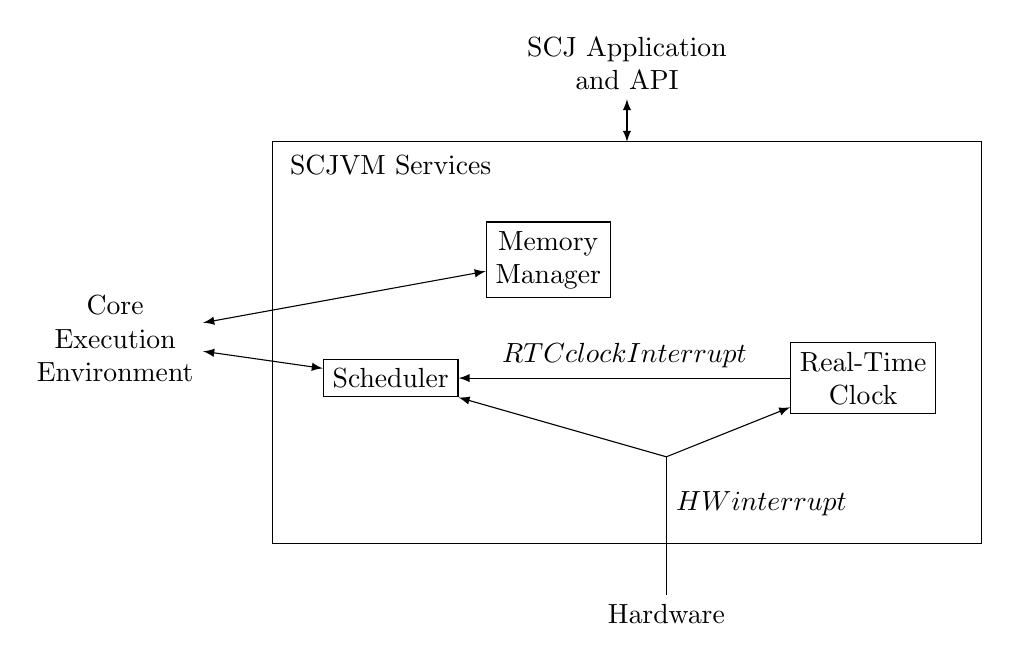
\begin{tikzpicture}
        \node[draw,align=center] (MM)  at (3.5cm,1.5cm) {Memory\\Manager};
        \node[draw,align=center] (S)   at (1.5cm,0cm)  {Scheduler};
        \node[draw,align=center] (RTC) at (7.5cm,0cm)  {Real-Time\\Clock};
        \draw (0cm,-2.1cm) rectangle (9cm,3cm);
        \node at (1.5cm,2.7cm) {SCJVM Services};
        
        \node[align=center] (HW) at (5cm,-3cm) {Hardware};
        
        \draw[-latex] (RTC) edge node[above] {$RTCclockInterrupt$} (S);
        
        \draw[-] (HW) -- node[above right] {$HWinterrupt$} coordinate[pos=1] (X) ++(0cm,2cm);
        \draw[-latex] (X) to (S);
        \draw[-latex] (X) to (RTC);
        
        \node[align=center] (CEE) at (-2cm,0.5cm) {Core\\Execution\\Environment};
        \draw[latex-latex] (S) -- (CEE);
        \draw[latex-latex] (MM) -- (CEE);
        
        \node[align=center] (App) at (4.5cm,4cm) {SCJ Application\\and API};
        \draw[latex-latex] (4.5cm,3cm) -- (App);
      \end{tikzpicture}
      \caption{The structure of the SCJVM services model, showing the
        channels used for communication between the processes in the
        model}
      \label{scjvm-services-model-fig}
\end{figure}

\chapter{The Core Execution Environment}
\label{cee-chapter}

This chapter describes the core execution environment (CEE) of an
SCJVM, which handles execution of an SCJ program.
% The CEE is aware of the structure of Java objects and classes in order
% to handle bytecode instructions properly.
In addition, the CEE of an SCJVM manages the flow of execution
dictated by the SCJ programming model, including, for example,
\texttt{Safelet} setup and mission execution.

This is the part of our SCJVM model that is handled by our compilation
strategy. 
So, it may take the form of a bytecode interpreter, which is the
starting point for the compilation, or C code, which is the output of
the compilation.
We describe both of these in this chapter
(Sections~\ref{cee-launcher-section}, \ref{cee-interpreter-section}
and~\ref{cee-c-code-section}) while the compilation strategy for
transforming between them is described in the next chapter.
We begin with an overview of the CEE's structure in the next section.
We conclude with some final considerations in
Section~\ref{cee-final-considerations-section}.

\section{Overview}

The CEE has three components, two of which depend on whether it is
interpreting bytecodes or executing C code. 
For the CEEs that use a bytecode interpreter, the components are
listed below and shown in Figure~\ref{cee-fig}:
\begin{itemize}
\item the object manager, which manages information about objects
  created during execution of the bytecode;
\item the interpreter itself, which handles execution of bytecode
  instructions; and
\item the launcher, which coordinates the startup of the SCJVM, the
  execution of missions, and the execution of methods in the
  interpreter.
\end{itemize}
% The interpreter is central to the main functionality of the core
% execution environment, but proper handling of infrastructure methods
% requires handling the SCJ mission-based programming model, which is
% dealt with by the launcher.
% The interpreter requires access to memory, but the class information
% and bytecode instructions do not change throughout the execution of
% the SCJVM, so they are provided as global constants in our model that
% are passed to the interpreter as parameters.
% Objects do change throughout the execution of the SCJVM and are in a
% separate region of memory to classes and bytecode instructions.
% The management of objects is handled by the object manager component
% of the core execution environment.

\begin{figure}[bth]
  \centering
  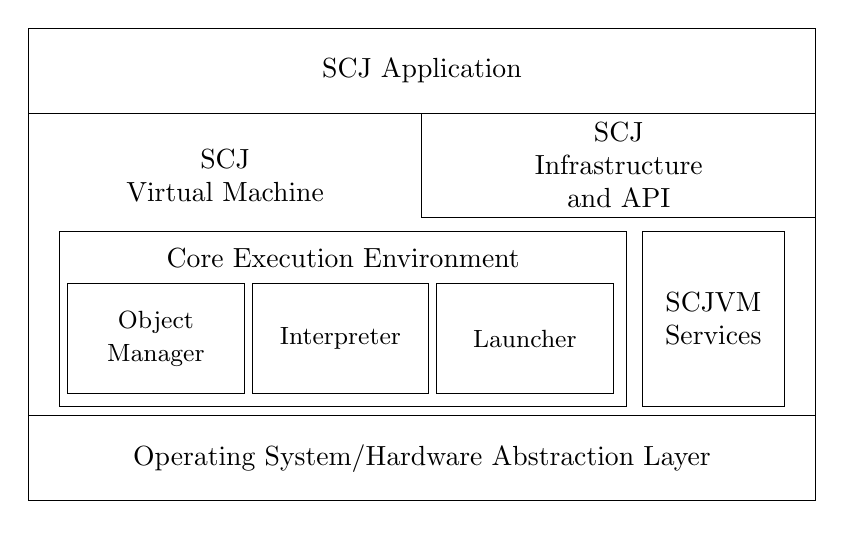
\begin{tikzpicture}

    \coordinate (width)  at (10cm,0cm);
    \coordinate (height) at (0cm,6cm);

    \path (0,0) -- (height)
    coordinate[pos=0.18] (OS boundary)
    coordinate[pos=0.20] (VM part bottom)
    coordinate[pos=0.57] (VM part top)
    coordinate[pos=0.60] (API boundary)
    coordinate[pos=0.82] (App boundary);
    
    \path (VM part bottom) -- (VM part top)
    coordinate[pos=0.7] (CEE part top);

    \path (VM part bottom) -- (VM part top)
    coordinate[pos=0.85] (CEE ypos);

    \path (0,0) -- (width)
    coordinate[pos=0.04] (CEE left)
    coordinate[pos=0.76] (CEE right)
    coordinate[pos=0.78] (VM Services left)
    coordinate[pos=0.96] (VM Services right)
    coordinate[pos=0.01] (CEE part sep);

    \path (CEE left) -- (CEE right)
    coordinate[pos=0.5] (CEE xpos);

    \path (0,0) to node[pos=0.5] (mid) {} (width);
    \path (0,0) to node[pos=0.25] (quart) {} (width);

    \draw (0,0) rectangle (width |- height);

    \draw (OS boundary) -- ++(width);
    \path (0,0) rectangle node[pos=0.5] (OS) {} (width |- OS boundary);
    \draw (mid |- API boundary) rectangle node[pos=0.5] (API) {} (width |- App boundary);
    \draw (App boundary) -- ++(width);
    \path (App boundary) rectangle node[pos=0.5] (App) {} (width |- height);

    \path (quart |- API boundary) rectangle node[pos=0.4] (SCJVM) {} (quart |- App boundary);
    \draw (CEE left |- VM part bottom) rectangle (CEE right |- VM part top);
    \draw (VM Services left |- VM part bottom) rectangle node[pos=0.5] (VM Services) {} (VM Services right |- VM part top);
    \coordinate (CEE) at (CEE xpos |- CEE ypos);

    \node[align=center] at (App)   {SCJ Application};
    \node[align=center] at (API)   {SCJ\\Infrastructure\\and API};
    \node[align=center] at (SCJVM) {SCJ\\Virtual Machine};
    \node[align=center] at (CEE)   {Core Execution Environment};
    \node[align=center] at (VM Services)  {SCJVM\\Services};
    \node[align=center] at (OS)    {Operating System/Hardware Abstraction Layer};

    \foreach \x in {1,...,3}
    \pgfmathsetmacro{\a}{0.33*(\x - 1)}
    \pgfmathsetmacro{\b}{0.33*\x}
    \path ($(CEE left) + (VM part bottom)!0.07!(VM part top)$) -- 
    node[pos=\a] (CEE part \x start) {}
    node[pos=\b] (CEE part \x end) {}
    ($(CEE right) + (VM part bottom)!0.07!(VM part top) - (CEE part sep)$);

    \foreach \x in {1,...,3} 
    \draw ($(CEE part \x start) + (CEE part sep)$)
    rectangle node[pos=0.5] (CEE part \x) {}
    (CEE part \x end |- CEE part top);
    
    \node[align=center] at (CEE part 1) {\small Object \\ \small Manager};
    \node[align=center] at (CEE part 2) {\small Interpreter};
    \node[align=center] at (CEE part 3) {\small Launcher};
  \end{tikzpicture}
  \caption{Structure of an SCJVM, showing the components of the CEE,
    and its relation to the SCJ infrastructure and the operating
    system/hardware abstraction layer}
  \label{cee-fig}
\end{figure}

The components after compilation to C are similar, but the object
manager is replaced with a struct manager, which manages C struct
types representing objects, and the interpreter is replaced with the C
program itself.
The launcher remains unchanged throughout the compilation.
It is assumed that it is already in the form of native code that can
be called from the C code.

The CEE is combined with the SCJVM services to form the complete
SCJVM; this is indicated in Figure~\ref{cee-fig}, which shows the same
structure described in Figure~\ref{scjvm-services-fig} in the previous
chapter, but has a focus on the CEE components.
The SCJVM services are unaffected by the compilation strategy and can
be implemented as a separate library.

Each of the components of the CEE is represented by a single \Circus{}
process in our model.
These processes interact as shown in Figure~\ref{cee-model-fig}.
The overall pattern of the interaction is unaffected by the
compilation, that is, the model of the compiled code has the same
overall flow of communication, although the components have different
names and different channels are used for communication.

\begin{figure}[ht]
  \centering
  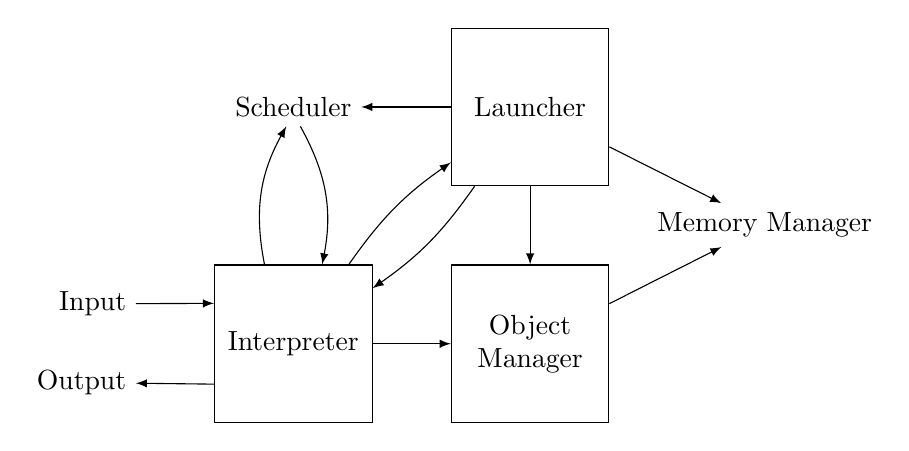
\begin{tikzpicture}
    \node[draw, minimum size=2cm, below right=2cm, align=center]
    (M) {Object\\Manager};
    \node[draw, minimum size=2cm, below=2cm]
    (I) {Interpreter};
    \node[draw, minimum size=2cm, right=2cm]
    (L) {Launcher};

    \draw[-latex, bend left=10] (I) edge (L);
    \draw[-latex, bend left=10] (L) edge (I);
    \draw[-latex] (I) edge (M);
    \draw[-latex] (L) edge (M);
    

    \node[below=1.5cm, right=4.5cm] (MM) {Memory Manager};
    \node[] (S) {Scheduler};
    \draw[-latex] (M) edge (MM);
    \draw (L) edge[-latex] (S);
    \draw (S) edge[-latex, bend left=20] (I);
    \draw (I) edge[-latex, bend left=20] (S);
    \draw (L) edge[-latex] (MM);

    \node[below=2.5cm, left=2cm] (In) {Input};
    \node[below=3.5cm, left=2cm] (Out) {Output};
    \draw[-latex] (In) to (I.153);
    \draw[-latex] (I.207) to (Out);
  \end{tikzpicture}
  \caption{The CEE model processes and their communication with each
    other and the SCJVM services}
  \label{cee-model-fig}
\end{figure}

The launcher manages the startup procedure for the SCJVM and the
execution of missions.
This involves communication with the interpreter (or C program) to
execute initialisation methods.
The interpreter then communicates back with the launcher when it
requires services that are provided by the SCJ infrastructure and API,
such as registering a schedulable object with the current mission.
Allocation of backing stores for the schedulable objects and entering
the corresponding memory areas involves communication with both the
object (or struct) manager in the CEE and the memory manager of the
SCJVM services.
The launcher must also communicate with the scheduler to indicate when
threads should be started or suspended during mission execution.

The interpreter must accept the requests to execute methods on the
main thread from the launcher, and it must also respond to requests
from the scheduler to start the other threads.
When a thread has finished execution, the interpreter signals to the
scheduler that the thread has finished so that it is no longer
scheduled.
The interpreter must also communicate with the launcher to handle
calls to methods that are provided by the SCJ infrastructure, such as
the methods to enter memory areas.
Handling of memory allocation during method execution is performed via
communication with the object manager, which then communicates with
the SCJVM memory manager.
Additionally, the interpreter communicates inputs and outputs to some
console input/output device, which is the only such device required by
the SCJ specification.
Supporting a full range of hardware connections is beyond the scope of
this work.

The interactions just described are modelled by channel
communications.
Those with the SCJVM services memory manager and scheduler use the
channels already described in
Sections~\ref{memory-manager-model-section}
and~\ref{scheduler-model-section}.
The types of values communicated by those channels are also used by
the CEE processes.
These include the type of object identifiers, $ObjectID$, the type of
thread identifiers, $ThreadID$, the type of backing store identifiers,
$BackingStoreID$, and the type of virtual machine data words, $Word$.
We also use the $ClassID$ and $MethodID$ types, which are the types of
class and method identifiers that are declared in the scheduler model
to permit the declaration of the $CEEstartThread$ channel.
Additionally, we declare a field identifier type, $FieldID$.
\begin{zed}
  [FieldID]
\end{zed}
The class, method and field identifiers may be the full names used in
Java class files or some shorter representation, such as unique
identification numbers.
In any case, type information needs to be taken into account so that
methods and fields with the same name, but different type signatures,
have different identifiers.
This is because the identifiers in Java class files include the type
information and the correct operation of method overloading relies on
it.

The channels used for communication between the CEE processes are
summarised in Figure~\ref{cee-channel-table}, with the full channel
declarations shown in Appendix~\ref{cee-model-channels}.
In addition to presenting the name and type for each channel, in the
first two columns of the table.
We also indicate which components of the CEE make use of the channel.
% L - launcher
% I - interpreter
% OM - object manager.
% I/L refers to a channel that is used by both the launcher and
% interpreter, with communications on that channel interleaved.
The channels $output$ and $input$ are used for communication with the
console device mentioned earlier.
As we do not model the console device itself, these are left as
externally visible channels when the component processes are composed
into the complete SCJVM model.
% The fact that they are external channels is indicated by the use of
% \textless{}ext.\textgreater{} in the final columns of the table.
Some channels are marked with various symbols (*, \dag{}, {}+{} and
\ddag{}) so that we can refer to them later in the text.

\begin{table}[t]
  \begin{center}
    \begin{tabular}{@{}lllll}
      \hline
      & Name & Parameter Type & \multicolumn{2}{l}{Communication} \\
      &      &                & from & to     \\
      \hline
      & $executeMethod$ & $ThreadID \cross ClassID \cross MethodID \cross \seq Word$ & L & I  \\
      & $executeMethodRet$ & $ThreadID \cross Word$ & I & L  \\
      & $continueExecution$ & $ThreadID$ & I & L \\
      & $initMainThread$ & $StackID$ & L & I \\ 
      *\dag & $register$ & $ThreadID \cross ObjectID$ & I & L \\
      %* & $registerRet$ & \textless no parameters\textgreater & L & I \\
      *\dag & $enterPrivateMemory$ & $ThreadID \cross \nat \cross ObjectID$ & I & L \\
      *\dag & $executeInAreaOf$ & $ThreadID \cross ObjectID \cross ObjectID$ & I & L \\
      *\dag & $executeInOuterArea$ & $ThreadID \cross ObjectID$ & I & L \\
      \dag & $enterPerReleaseMemory$ & $ThreadID \cross ObjectID$ & I & L \\
      {}+{} & $suspend$ & \textless no parameters\textgreater & I & L \\
      {}+{} & $suspendRet$ & \textless no parameters\textgreater & L & I \\
      {}+{} & $resumeThread$ & $ThreadID$ & I & L \\
      {}+{} & $resumeThreadRet$ & \textless no parameters\textgreater & L & I  \\
      & $output$ & $Word$ & I & \textless ext.\textgreater \\
      & $input$ & $Word$ & \textless{}ext.\textgreater{} & I \\
      & $enterBackingStore$ & $ThreadID \cross BackingStoreID$ & L & OM \\
      & $exitBackingStore$ & $ThreadID$ & L & OM  \\
      & $exitBackingStoreRet$ & $BackingStoreID \cross \boolean$ & L & OM \\
      & $getCurrentAC$ & $ThreadID$ & L & OM \\
      & $getCurrentACRet$ & $BackingStoreID$ & OM & L \\
      & $newObject$ & $ThreadID \cross ClassID$ & I/L & OM  \\
      & $newObjectRet$ & $ObjectID$ & OM & I/L  \\
      \ddag & $getClassIDOf$ & $ObjectID \cross ClassID$ & I/L & OM  \\
      \ddag & $getField$ & $ObjectID \cross FieldID$ & I & OM \\
      \ddag & $getFieldRet$ & $Word$ & OM & I \\
      \ddag & $putField$ & $ObjectID \cross FieldID \cross Word$ & I & OM \\
      \ddag & $getStatic$ & $ClassID \cross FieldID$ & I & OM \\
      \ddag & $getStaticRet$ & $Word$ & OM & I \\
      \ddag & $putStatic$ & $ClassID \cross FieldID \cross Word$ & I & OM \\
      & $addThreadMemory$ & $ThreadID \cross BackingStoreID$ & I & OM \\
      & $removeThreadMemory$ & $ThreadID$ & I & OM \\       
      \hline
    \end{tabular}
  \end{center}
  \caption{The channels used for communication between CEE processes
    before compilation. 
    In the final two columns, L refers to the launcher, I refers to
    the interpreter, OM refers to the object manager, I/L indicates a
    channel shared by the interpreter and launcher in interleaving,
    and \textless{}ext.\textgreater{} indicates and external channel.}
  \label{cee-channel-table}
\end{table}

Most of the channels are part of pairs, with one channel to
communicate a signal to begin an operation and supply any inputs, and
a return channel to communicate back when the operation has finished
and supply any outputs.
The return channel is named by appending $Ret$ to the name of the
channel used to initiate the operation.

There are some channels that deviate this pattern of having a return
channel.
The $executeMethod$ channel is used to signal to the interpreter that
it should begin execution of a method on a given thread.
The interpreter signals on $executeMethodRet$ channel when it has
finished execution of the method.
Since the launcher may need to take some action, such as exiting a
memory area, after the interpreter has finished executing a method,
the interpreter waits until it receives a signal on the
$continueExecution$ channel before continuing to execute.
Since the $continueExecution$ channel forms part of this communication
pattern, it does not have its own return channel.

Before the interpreter can execute methods on the $main$ thread, the
stack space for the $main$ thread must allocated by the launcher and
communicated to the interpreter.
This is handled by the $initMainThread$ channel, which carries the
$StackID$ for the stack space allocated for the $main$ thread.
The interpreter waits for communication on the $executeMethod$ channel
before commencing execution, so the launcher does not need to wait for
the interpreter to finish registering the $main$ thread's stack.

As mentioned above, while executing a method, the interpreter may
signal back to the launcher for handling of special methods.
The channels used for this are the ones marked with a * or a {}+{} in
Table~\ref{cee-channel-table}.
The channels marked with a * represent calls to infrastructure methods
that are part of the SCJ API.
The inputs and outputs of these methods (and hence the types of the
channels associated with them) are taken from the SCJ specification.
The channels marked with a \dag{} are methods that do not return a
value and involve execution of a method in the interpreter as part of
their handling.
Thus, the interpreter waits for a signal on the $executeMethod$
channel after signalling the launcher to handle one of these methods.
The methods marked with a \dag{} do not, therefore, require separate
return channels.
The channels marked with a + expose SCJVM scheduler operations to the
code executed in the interpreter, in order to allow for the
implementation of event handlers. 
Their types follow those of the scheduler's channels.

As mentioned previously, the $output$ and $input$ channels are used to
communicate $Word$ values to and from a console device.
The rest of the channels are used by the launcher and the interpreter
to communicate with the object manager.
The $enterBackingStore$ channel is used by the launcher to signal to
the object manager when a memory area is entered so that it can record
that the corresponding backing store has been entered.
This carries the $ThreadID$ of the thread to be entered, since the
backing stores entered are recorded separately for each thread, and
the $BackingStoreID$ of the backing store to be entered.
There is no corresponding return channel, since it is not necessary
for the launcher to wait while the object manager records the entry to
a backing store.
Similarly, the $exitBackingStore$ channel is used to signal an exit
from the backing store that is the current allocation context of the
given thread.
This does have a return channel, since the launcher must be informed
if the backing store was cleared due to no longer being in use by any
thread.
The $BackingStoreID$ of the exited backing store and a boolean value
indicating if the backing store was cleared are therefore communicated
back to the launcher on a return channel.
Additionally, the $getCurrentAC$ channel (and its return channel) is
used to obtain the $BackingStoreID$ of the backing store used as the
current allocation context for given thread from the object manager,
in order to handle some cases of entering memory areas.

The remaining channels used by the launcher to communicate with the
object manager are used by both the launcher and the interpreter.
These are the $newObject$ channel, which is used to allocate space for
new objects in the current allocation context, and the $getClassIDOf$
channel, which is used to obtain the $ClassID$ for the class of the
object associated with a given $ObjectID$.
% It is used for implementing the \texttt{new} bytecode in the
% interpreter and for creating infrastructure objects in the launcher.
% After compilation it represents a call to a method similar to
% \texttt{malloc()}.
The $newObject$ channel carries the $ThreadID$ of the current thread,
since there is a separate allocation context for each thread, and the
$ClassID$ of the class of the object to be allocated.
The object manager returns the $ObjectID$ of the newly allocated
object via the corresponding return channel.
The $getClassIDOf$ channel carries both the input and output to the
operation on the same channel, since it is a simple data accessing
operation that can be dealt with in a single communication.

The other channels used by the interpreter are the channels for
accessing fields of objects and classes.
The $getField$ channel is used for obtaining the value stored in a
given field of a given object.
It carries the $ObjectID$ of the object whose field is to be accessed
and the $FieldID$ of the field to be accessed.
The object manager then returns the $Word$ value stored in the field.
For putting a value into an object's field, the $putField$ channel is
used, which carries the $Word$ value to store in the field in addition
to the $ObjectID$ and $FieldID$ that identify the object and field to
update.
As this just updates the field and does not return any information,
there is no need for a return channel.
Channels for accessing static fields, $getStatic$ and $putStatic$, are
also provided.
These operate similarly to the channels for object fields but use
$ClassID$ values rather than $ObjectID$ values, since static fields are
attached to classes rather than objects.

The final channels used by the interpreter are the $addThreadMemory$
and $removeThreadMemory$ channels.
The $addThreadMemory$ is used to inform the object manager of a
thread's initial allocation context when the thread starts.
It carries the $ThreadID$ of the thread and the $BackingStoreID$ of
the backing store that serves as the thread's initial allocation
context.
When a thread has finished execution, it informs the object manager
via the $removeThreadMemory$ channel, which carries the $ThreadID$ of
the thread.

As mentioned earlier, some channels used by the interpreter to
communicate with the object manager are replaced with different
channels during compilation.
Those channels are marked with a \ddag{} in
Table~\ref{cee-channel-table}.
After compilation these channels are replaced with channels to obtain
the struct representing the contents of an object and to store an
object’s struct after updating it.
Note that the $getClassIDOf$ channel is shared between the launcher
and interpreter.
After compilation, the interpreter accesses a struct field storing the
$ClassID$ for an object.
However, the launcher is unaffected by the compilation and is agnostic
as to whether the program is in the form of bytecode or C code.
Therefore, the launcher continues to use the $getClassIDOf$ channel
after compilation, which represents a service offered by the object
manager or struct manager to obtain the $ClassID$ by whatever means
are appropriate to the form of the object.
As an optimisation in an implementation, the launcher could be changed
to access struct fields in the same way as the interpreter.
We discuss the form of field accesses in the C code and the channels
used for them in more detail in
Sections~\ref{cee-struct-manager-subsection}
and~\ref{cee-c-program-subsection}.

%\input{../../SCJ-VM/James/LIchans.zed}

%\input{../../SCJ-VM/James/memory_chans.zed}


Next, in Section~\ref{cee-launcher-section}, we describe our model of
the launcher.
We then detail the bytecode interpreter model in
Section~\ref{cee-interpreter-section}, and the C code model in
Section~\ref{cee-c-code-section}.

\section{Launcher}
\label{cee-launcher-section}

As mentioned in the previous section, the launcher is the component of
the CEE that manages the SCJVM startup and coordinates mission
execution.
It is described by the $Launcher$ process.

The launcher remains unaffected throughout the compilation strategy,
because it is agnostic to the class and bytecode information.
However, the launcher must know where to begin execution, so it takes
a parameter, $safeletClass$, which is the $ClassID$ of the
\texttt{Safelet} class.
This can be seen in the the $Launcher$ process definition, the
beginning of which is shown below.

Class initialisers must be executed as part of the SCJVM startup
procedure.
The order in which they are executed is determined by the dependencies
between class initialisers and classes, and is passed to the
$Launcher$ process as a second parameter, $initOrder$, which is a
sequence of $ClassID$s.
\begin{circus}
  \circprocess Launcher \circdef safeletClass : ClassID; initOrder : \seq ClassID \circspot \circbegin
\end{circus}

In what follows, we describe the definition of $Launcher$, focusing on
the aspects relevant for the compilation.
The complete definition can be found in
Appendix~\ref{launcher-appendix}.

The state of the $Launcher$ is divided into three parts.
The first part contains the identifiers of the objects that form the
SCJ mission model, so that the $Launcher$ can call methods of those
objects during SCJVM startup.
The second part contains information on the memory-area objects of
the program, including the relationship between the memory-areas and
the backing stores they represent, so that methods for entering and
exiting memory-areas can be handled.
The final part of the state describes the relationship between the
schedulable objects of SCJ and the threads used by the CEE so that the
threads can be started when mission execution begins.

We use separate Z schemas to specify each part of the state.
The first part is described by the $MissionManager$ schema, shown
below.
It contains the identifiers of three objects:
\begin{itemize}
\item $safelet$, the instance of the class implementing the
  \texttt{Safelet} interface for the program;
\item $missionSequencer$, the mission sequencer
  returned by the safelet's \texttt{getSequencer()} method; and
\item $currentMission$, the mission that is currently executing.
\end{itemize}
Methods of these objects are called at various points throughout SCJVM
startup and mission execution.
\begin{schema}{MissionManager}
  safelet, missionSequencer, currentMission : ObjectID
\end{schema}

The second part of the $Launcher$'s state is described by the
$MemoryAreaManager$ schema below.
It contains the identifiers of the memory-area objects for the
immortal memory, $immortalMemory$, and mission memory,
$missionMemory$.
There is a map, $backingStores$, that relates these identifiers and
the identifiers of the other memory-area objects, to the identifiers
of the backing stores they represent.
We also record the backing store identifiers of the per-release
memories for each thread in the $perReleaseMemories$ map.
Finally, to make sure that nested private memories can be reused,
there is a map from backing store identifiers to the identifiers of
private backing stores they contain, $privateMemoryMap$.
\begin{schema}{MemoryAreaManager}
  immortalMemory, missionMemory : ObjectID \\
  backingStores : ObjectID \finj BackingStoreID \\
  perReleaseMemories : ThreadID \finj BackingStoreID \\
  privateMemoryMap : BackingStoreID \finj BackingStoreID
\where
  \cdots
\end{schema}
Each of the maps in the $MemoryAreaManager$ is injective, since each
memory-area object has a distinct backing store and memory-areas
cannot share a nested private memory-area.
The invariants of $MemoryAreaManager$ are elided above. 
They ensure that each memory-area object has a corresponding backing
store in $backingStores$, and that areas which are not nested private
memories do not appear in the range of $privateMemoryMap$.

The final part of the state is specified in the $SchedulableManager$
schema below.
It contains a map, $schedulableThreads$, from the identifiers of
schedulable objects to the identifiers of the threads associated with
them.
This map must be injective, since every schedulable object has a
separate thread.
\begin{schema}{SchedulableManager}
  schedulableThreads : ObjectID \finj ThreadID
\end{schema}

The state of the process is then the conjunction of these three
schemas.
\begin{circusaction}
  \circstate LauncherState == MissionManager \land MemoryAreaManager \land SchedulableManager
\end{circusaction}

The $Launcher$ state is initialised as described in $LauncherInit$,
which is shown below.
The object identifiers are initialised to the $null$ identifier.
They are later filled with non-$null$ identifiers as the corresponding
objects are created during SCJVM execution.
Similarly, each of the maps is initialised to the empty set.
\begin{schema}{LauncherInit}
	LauncherState~'
\where
	\{ safelet', missionSequencer', currentMission', immortalMemory', missionMemory' \} \\
	\t1 {} \subseteq \{ null \} \\
	backingStores' = \emptyset \\
	perReleaseMemories' = \emptyset \\
	privateMemoryMap' = \emptyset \\
	schedulableThreads' = \emptyset
\end{schema}

The main action of the $Interpreter$ proceeds as shown below.
The state is first initialised as described by $LauncherInit$ and then
the actions $Startup$ and $RunNextMission$ follow in sequence.
$Startup$ defines the SCJVM startup procedure that must be performed
once at the start of SCJVM execution, whereas $RunNextMission$ defines
the procedure that must be performed for each mission run.
We do not handle mission termination in our $Launcher$ model.
This is because the SCJ mission termination procedure has almost no
effect on our compilation strategy; a single mission is sufficient for
our examples to evaluate the compilation strategy.
A formal account of it is available elsewhere~\cite{cavalcanti2013,
  luckcuck2016, zeyda2011}. 
Thus, $RunNextMission$ is only executed once.
\begin{circusaction}
  \circspot \lschexpract LauncherInit \rschexpract \circseq Startup \circseq RunNextMission
\end{circusaction}

The definition of $Startup$ is shown below.
It performs a number of actions in sequence, following the startup procedure for an SCJVM:
\begin{itemize}
\item creating the main thread's stack and passing on the
  $initMainThread$ channel, in $MakeMainStack$;
\item executing the class initialisers in the order given in
  $initOrder$, in $RunClassInitialisers$;
\item creating the immortal memory object that corresponds to the root
  backing store and storing it in $immortalMemory$, in
  $CreateImmortalMemory$;
\item creating the \texttt{Safelet} object and storing it in
  $safelet$, in $CreateSafelet$;
\item calling the \texttt{immortalMemorySize()} and
  \texttt{globalBackingStoreSize()} methods of the $safelet$, and
  checking that the size of the root backing store matches those
  values, in $CheckImmortalMemory$ and $CheckRemainingBackingStore$;
\item calling the \texttt{initializeApplication()} method of the $safelet$, in $InitializeApplication$;
\item calling the $safelet$'s \texttt{getSequencer()} method and
  storing the returned value in $missionSequencer$, in $GetSequencer$;
  and
\item creating the $missionMemory$ object with its corresponding backing store, in $CreateMissionMemory$.
\end{itemize}
\begin{circusaction}
  Startup \circdef MakeMainStack \circseq RunClassInitialisers \circseq CreateImmortalMemory \circseq CreateSafelet \circseq \\
  \t1 CheckImmortalMemory \circseq CheckRemainingBackingStore \circseq InitializeApplication \circseq \\
  \t1 GetSequencer \circseq CreateMissionMemory
\end{circusaction}

$RunNextMission$ begins with calling the \texttt{getNextMission()}
method of $missionSequencer$, in the action $GetNextMission$.
The returned mission is stored in $currentMission$.
Its \texttt{missionMemorySize()} method is then executed, and the
backing store of $missionMemory$ is resized to match, in
$ResizeMissionMemory$.
Next, in $InitializeMission$, the mission's \texttt{initialize()}
method is executed, during which the schedulable objects for the
mission are registered.
Afterwards, in $InitialiseAndStartThreads$, the registered schedulable
objects have their stacks and backing stores created, after which the
threads for all the schedulable objects are started.
Finally, in $WaitForExecution$, the $main$ thread suspends itself and
the $Launcher$ then waits, handling special methods for the threads of
the program when necessary.
Since termination is not handled, this phase of the program continues
indefinitely.
\begin{circusaction}
  RunNextMission \circdef GetNextMission \circseq ResizeMissionMemory \circseq InitializeMission \circseq \\
  \t1 InitialiseAndStartThreads \circseq WaitForExecution
\end{circusaction}

During these actions, methods are executed using the channels
$executeMethod$, $executeMethodRet$ and $continueExecution$, discussed
earlier.
The identifiers of the methods, which may be standard methods from the
SCJ API, or implementation-defined API methods required by the
launcher, are represented by constants in the model.
Although most of the methods used by the $Launcher$ are executed
simply by communicating on each of the channels mentioned above in
turn, as noted above, in $InitializeMission$, the
\texttt{initialize()} method of a mission requires handling of the
\texttt{register()} method for each schedulable object.
We must also provide handling for other special methods.
This is done in the $HandleSpecialMethodsMainLoop$ action below, which
offers handling of the special methods while waiting for return from
the \texttt{initialize()} method on the $executeMethodRet$ channel.
A similar action, without the final choice accepting
$executeMethodRet$, is used to handle special methods in
$WaitForExecution$.
\begin{circusaction}
  HandleSpecialMethodsMainLoop \circdef \circval memoryEntries : ThreadID \fun \nat; \circres retVal : Word \circspot \\
  \t1 (\Extchoice t : ThreadID \circspot \\
  \t2 EnterMemory(t) \circseq \\
  \t2 HandleSpecialMethodsMainLoop(memoryEntries \oplus \{ t \mapsto memoryEntries~t + 1 \}, retVal)) \\
  \t1 {} \extchoice {} \\
  \t1 (\Extchoice t : ThreadID \circspot \\
  \t2 \lcircguard memoryEntries~t > 0 \rcircguard \circguard ExitMemory(t) \circseq \\
  \t2 HandleSpecialMethodsMainLoop(memoryEntries \oplus \{ t \mapsto memoryEntries~t - 1 \}, retVal)) \\
  \t1 {} \extchoice {} \\
  \t1 ((Register \extchoice Suspend \extchoice Resume) \circseq \\
  \t2 HandleSpecialMethodsMainLoop(memoryEntries, retVal)) \\
  \t1 {} \extchoice {} \\
  \t1 (\lcircguard \forall t : ThreadID @ memoryEntries~t = 0 \rcircguard \circguard {} \\
  \t2 executeMethodRet?thr \prefixcolon (thr = main) ?r \then continueExecution!main \then retVal := r)
\end{circusaction}
$HandleSpecialMethodsMainLoop$ takes a value parameter,
$memoryEntries$, which is a map recording how many times a memory area
has been entered for each thread.
It also take a value parameter, $retVal$, which captures the return
value from the execution of the method on the $main$ thread.
It offers a choice of handling a memory-area entry, handling the
corresponding memory-area exit, handling a special method that does
not enter memory-areas, or accepting return from the execution of the
method on the $main$ thread (handled in the usual way using
$executeMethodRet$ and $continueExecution$, with the return value
stored in $retVal$).

$HandleSpecialMethodsMainLoop$ handles memory-area entering
methods, which execute another method after entering a memory-area,
during which further special methods may be called.
Each entry to a memory-area must be matched by a corresponding exit
from the memory-area when this extra method execution returns.
Thus, the entries to memory-areas are tracked in the $memoryEntries$
map.

The number stored in $memoryEntries$ for a thread identifier $t$ is
incremented after handling a memory-area entry on that thread as
described in $EnterMemory(t)$.
Similarly, it is decremented after handling exit from the memory-area
in $ExitMemory(t)$, which is only offered if the value is already
greater than zero.
After handling memory-area entry or exit, or another special method
(handled in the actions $Register$, $Suspend$ and $Resume$),
$HandleSpecialMethodsMainLoop$ recurses to allow further special
methods to be handled.
The return from the top-level method execution on the $main$ thread is
only permitted once all memory areas have been exited and
$memoryEntries$ is zero for all threads.

To illustrate how the nested method execution after memory-area entry
is performed, we show the $ExecuteInAreaOf$ action below, which is one
of the actions offered in external choice in $EnterMemory$, along with
actions to handle other memory-area entering operations.
$ExecuteInAreaOf$ takes a thread identifier $thread$ as a parameter
and only accepts communications from that thread, so that we can
separate out memory-area entries for each thread.
The identifier of a \texttt{Runnable} object, $runnable$, is received
via the $executeInAreaOf$ channel, which is the object that indicates
the method to be executed in the memory-area. 
Such an identifier is received for all of the memory-area entering
methods.
In the case of $ExecuteInAreaOf$, another identifier, $object$, is
also received and a $FindBackingStore$ action is used to communicate
with the memory manager to determine its backing store.
This backing store is then entered, via communication on the
$enterBackingStore$ channel.
The class of the $runnable$ object is determined and its
\texttt{run()} method (represented here by the $run$ identifier) is
executed by signalling on the $executeMethod$ channel.
No communication on the $executeMethodRet$ channel is waited for in
this action, because it is handled separately in the $ExitMemory$
action since other special methods (including further memory entries)
may occur inbetween.
\begin{circusaction}
  ExecuteInAreaOf \circdef \\
  \t1 \circval thread : ThreadID \circspot \circvar runnable, object : ObjectID; bs : BackingStoreID \circspot \\
  \t1 executeInAreaOf?t \prefixcolon (t = thread) ?obj?r \then object, runnable := obj, r \circseq \\
  \t1 FindBackingStore(object, bs) \circseq \\
  \t1 enterBackingStore!thread!bs \then getClassIDOf!runnable?runnableClass \\
  \t1 {} \then executeMethod!thread!runnableClass!run!(\langle runnable \rangle) \then \Skip
\end{circusaction}
The return from the \texttt{run()} method, and the exit from the
memory-area, is specified by the $ExitMemory$ action below.
This, as with the $ExecuteInAreaOf$ action, takes a $thread$
parameter.
A return from a method executing on that thread is accepted on the
$executeMethodRet$ channel, and its return value is discarded as the
\texttt{run()} method is \texttt{void}.
The exit from the memory-area is then performed using the
$exitBackingStore$ and $exitBackingStoreRet$ channels.
The $Launcher$ state may afterwards be updated to account for the
exited memory-area being cleared (due to no longer being in use by any
thread), which is specified in the $ClearPrivateMemory$ schema.
After the exit from the memory-area has been handled, the $Launcher$
signals that normal execution on $thread$ may continue using the
$continueExecution$ channel.
\begin{circusaction}
  ExitMemory \circdef \circval thread : ThreadID \circspot \\
  \t1 executeMethodRet?t \prefixcolon (t = thread) ?void \\
  \t1 {} \then exitBackingStore!thread \then exitBackingStoreRet?bsid?isCleared \then {} \\
  \t1 \circif isCleared = \true \circthen \lschexpract ClearPrivateMemory[bsid/toClear?] \rschexpract \\
  \t1 {} \circelse isCleared = \false \circthen \Skip \\
  \t1 \circfi \circseq continueExecution!thread \then \Skip
\end{circusaction}

The \texttt{register()} method also needs to execute a method in the
interpreter to obtain a thread's priority.
Further special methods are not handled in this case, since the method
to obtain a thread's priority is expected to be a simple method that
does not call special methods.

This handling of special methods is used by the interpreter process
(or C program, after compilation), which must communicate with the
$Launcher$ when such methods are encountered.
To allow for the behaviour of executing methods after entering memory
areas (or during the \texttt{register()} method), the interpreter must
also be prepared to execute another method after signalling to the
$Launcher$.
This is transformed to nested method executions during the compilation
strategy in order to preserve the communication pattern with the
$Launcher$.
We describe in more detail how this communication is performed in the
interpreter in Section~\ref{cee-interpreter-subsection}, and in C
program in Section~\ref{cee-c-program-subsection}.
In the next section, we describe the bytecode interpreter, which,
along with the $Launcher$, forms the CEE before the application of the
compilation strategy.

% \input{../../SCJ-VM/James/launcher.zed}

\section{Bytecode Interpreter Model}
\label{cee-interpreter-section}

This section describes the bytecode interpreter that handles execution
of an SCJ bytecode program.
Its model is composed of two processes:~the model of the object
manager, $ObjMan$, and the model of the interpreter itself,
$Interpreter$.
These are composed together in parallel with the $Launcher$ to form
the complete core execution environment, $CEE$, as shown below.
The synchronisation sets and channel hidings, omitted here, are
consistent with the communication patterns shown in
Table~\ref{cee-channel-table}.
The parameters of each of the components, including the classes, $cs$,
and bytecode instructions, $bc$, which are explained later in this
section, become parameters of $CEE$.
\begin{circus}
  CEE(cs,bc,sid,initOrder) \circdef ObjMan(cs) \parallel
  Interpreter(cs,bc) \parallel Launcher(sid,initOrder)
\end{circus}

In Section~\ref{cee-bytecode-subset-subsection}, we first give an
informal description of the bytecode instructions handled in our model
and the ways in which their SCJ semantics differ from that of standard
Java.
In Section~\ref{cee-classes-subsection}, we describe our model of Java
class information that is used by both $ObjMan$ and $Interpreter$.
The first component, $ObjMan$, is described in
Section~\ref{cee-object-manager-subsection} and the second,
$Interpreter$, in Section~\ref{cee-interpreter-subsection}.

\subsection{Bytecode Subset}
\label{cee-bytecode-subset-subsection}

We model a subset of Java bytecode sufficient to express a wide
variety of SCJ programs and illustrate how further features may be
added, but small enough to permit effective reasoning.
The subset has been chosen by considering the bytecode generated from
a simple SCJ program and removing instructions similar to those
already in the subset.
This ensures the model is not unnecessarily complicated with trivial
or redundant instructions, so we can concentrate on the instructions
that are most of interest in creating the compilation strategy.
The bytecode instructions in our subset are described in
Table~\ref{bytecode-subset-table}.

\begin{table}
  \centering
  \begin{tabular}{llp{8.5cm}}
    \hline
    Instruction & Parameter & Description \\
    \hline
    \texttt{aconst\_null} & (none) & 
    Pushes a null object reference onto the operand stack.
    \\
    \texttt{aload} & local variable index &
    Loads the value from a specified local variable and pushes it
    onto the operand stack.
    \\
    \texttt{areturn} & (none) &
    Returns from the current method, pushing the value on top of the
    current method's operand stack onto the operand stack of the
    method returned to.
    \\
    \texttt{astore} & local variable index &
    Pops a value from the operand stack and stores it in the specified
    local variable.
    \\
    \texttt{dup} & (none) &
    Duplicates the value on top of the operand stack.
    \\
    \texttt{getfield} & constant pool index &
    Pops an object reference from the operand stack, gets the value of
    the field specified by the identifier at the given constant pool
    index for the referenced object, and pushes it onto the operand
    stack.
    \\
    \texttt{getstatic} & constant pool index &
    Gets the value of the static field specified by the field and
    class identifiers at the given constant pool index, and pushes it
    onto the operand stack.
    \\
    \texttt{goto} & program address &
    Unconditionally branches to the given program address.
    \\
    \texttt{iadd} & (none) &
    Pops two integer values from the operand stack, adds them, and
    pushes the result onto the operand stack.
    \\
    \texttt{iconst} & integer value &
    Pushes the given integer value onto the operand stack of the
    current method.
    \\
    \texttt{if\_icmple} & program address &
    Pops two integer values from the operand stack, and branches to
    the given program address if the second value popped is less than
    or equal to the first value.
    \\
    \texttt{ineg} & (none) &
    Pops an integer value from the operand stack, negates it, and
    pushes the negated value onto the operand stack.
    \\
    \texttt{invokespecial} & constant pool index &
    Gets the method and class identifier at the given constant pool
    index and invokes the specified method of the specified class,
    popping the method's arguments, plus a \texttt{this} object
    reference, from the operand stack.
    \\
    \texttt{invokestatic} & constant pool index &
    Gets the method and class identifier at the given constant pool
    index and invokes the specified method of the specified class,
    popping the method's arguments from the operand stack.
    \\
    \texttt{invokevirtual} & constant pool index &
    Gets the method and class identifier at the given constant pool
    index, pops the arguments of the specified method, including a
    \texttt{this} object reference, from the operand stack, and
    invokes the specified method of the class of referenced object.
    \\
    \texttt{new} & constant pool index &
    Allocates a new object of the class specified by the identifier at
    the given constant pool index and pushes a reference to the new
    object onto the operand stack.
    \\
    \texttt{putfield} & constant pool index &
    Pops an object reference and value from the operand stack and
    stores the value in the field specified by the identifier at the
    given constant pool index for the referenced object.
    \\
    \texttt{putstatic} & constant pool index &
    Pops a value from the operand stack and stores the value in the
    static field specified by the field and class identifiers at the
    given constant pool index.
    \\
    \texttt{return} & (none) &
    Returns from a method with no return value.
    \\
    \hline
  \end{tabular}
  \caption{The instructions in our bytecode subset}
  \label{bytecode-subset-table}
\end{table}

Java bytecode instructions operate over a state that records
information on all loaded classes, a stack frame, and the object data
residing in memory.
Various pieces of class information are required for execution of
bytecode instructions, but a constant pool, which stores all the
constants and names required by the class, is the main information
used.

The constant pool contains references to classes, methods and fields
used by the bytecode instructions in the class, as well as constant
values used in the code.
The form of the constant pool is a large array.
Indices into this array are used as parameters to instructions
requiring information from the constant pool.
For example, the \texttt{getfield} and \texttt{putfield} instructions
take constant pool index parameters pointing to a reference to a field
whose value should be obtained or set.
Other class information used at runtime includes information on fields
and methods belonging to the class, which is required for creation of
objects and invocation of methods.

The frame stack forms the second part of the JVM manipulated by
bytecode instructions and consists of a series of frames that contain
the runtime information for each invocation of a method.
When a method is invoked, a new stack frame is created for it and
pushed onto the frame stack, and when the method returns, the stack
frame is popped from the stack.

Each stack frame contains an operand stack, which is used to store
values manipulated by bytecode instructions, and an array of local
variables.
Most bytecode instructions manipulate the operand stack in some way,
popping arguments from it, pushing results to it or performing
specific operations upon it.

The local variables are used to store the arguments of a method and
the results of computations performed on the operand stack.
Operations are not performed directly on the local variables, so the
only bytecode instructions that affect them are those for moving
values between the operand stack and the local variables
(\texttt{aload} and \texttt{astore} are examples of such
instructions).

Some bytecode instructions also manipulate objects, which in our case
reside in backing store memory.
Such instructions include \texttt{new}, which creates objects, and
\texttt{getfield}, which gets the value from a field of an object.
In our choice of instructions for the subset, we mainly focus on
manipulation of objects and method invocation, since those are core
concepts of Java bytecode and require special handling by the
compilation strategy.

The instruction \texttt{dup} is included as an example of a simple
instruction that operates on the operand stack.
It has been chosen for its frequent occurrence in object initialisation.
Other instructions that do simple operand stack manipulation,
including the arithmetic instructions, can be specified similarly.

We also include a few arithmetic instructions as an example of how
integers are handled.
Specifically, we include the integer addition operation,
\texttt{iadd}, as an example of a binary operation, and the integer
negation operation, \texttt{ineg}, as an example of an unary
operation.
We do not include operations for floating point values since the
operations upon them are not substantially different from those on
integers at the level of modelling and compilation.
The model can be easily extended to include more integer operations.

Instructions that create object references (the \texttt{new} and
\texttt{aconst\_null} instructions), pass them around (\texttt{aload},
\texttt{astore}, \texttt{areturn}, etc.), and permit
field accesses (\texttt{getfield} and \texttt{putfield}) are also
included to allow the full range of object manipulations.
We also provide instructions for \texttt{static} field accesses
(\texttt{getstatic} and \texttt{putstatic}) since they are of use in
sharing data between different parts of the program.
However, arrays are not included as they require additional
instructions and can be emulated, albeit inefficiently, with the
instructions given here.

Both the \texttt{invokevirtual} and \texttt{invokespecial}
instructions, which invoke methods on objects, are included.
The \texttt{invokevirtual} instruction looks up the method to invoke
in the method table for the class of the object that the method is
invoked on.
The \texttt{invokespecial} instruction, on the other hand, uses the
class identifier supplied in the method reference pointed to by the
parameter of the instruction when looking up the method.
The \texttt{invokestatic} instruction, for invoking \texttt{static}
methods of classes, is similar to \texttt{invokespecial}, but does not
supply a \texttt{this} object parameter, whereas
\texttt{invokevirtual} and \texttt{invokespecial} pop \texttt{this}
from the stack as an extra argument.

The \texttt{goto} and \texttt{if\_icmple} instructions are provided as
examples of control flow instructions, with \texttt{goto} representing
an unconditional branch and \texttt{if\_icmple} representing a
conditional branch.
Other forms of conditional branch may be implemented in a similar
fashion to \texttt{if\_icmple}, but we do not include those in our
subset since \texttt{if\_icmple} is sufficient to represent most
control flow structures.
Although \texttt{goto} could be represented as a special case of
\texttt{if\_icmple}, we include it as a separate instruction due to
its frequent use in conjunction with \texttt{if\_icmple} to implement
loops.

We do not handle exceptions; errors in the SCJVM are instead handled
by simply aborting execution.
SCJ programs can be statically verified to prove that exceptions will
not be thrown~\cite{kalibera2010,marriott2014}.
Furthermore, reliance on exceptions to handle errors has been
discouraged by an empirical study due to the potential for errors in
exception handling~\cite{sawadpong2012}.
The bytecode instructions that relate to throwing and catching
exceptions are, therefore, not included in our bytecode subset.

As a simplifying assumption, we consider that all values consist of
only a single virtual machine word.
This means that \texttt{long} and \texttt{double} values are not
handled.
Any SCJ API methods that take \texttt{long} or \texttt{double}
arguments are viewed as taking \texttt{int} or \texttt{float} instead.
The reason for this assumption is that handling of two word values
makes little difference at the level of the formal model and our
approach can be easily extended to deal with more types.

Further, we do not make a distinction between the different virtual
machine types in our bytecode instructions.
This is justified as the bytecode instructions simply handle values as
32-bit words, with the type information only used for typechecking
during bytecode validation. 
The code passed into the core execution environment is assumed to have
already passed, which may be done by a separate
component~\cite{klein2003, stark2001, coglio2000, xavier2003}). 
Since many of the instructions behave the same for different types, we
only include those instructions that handle values as object
references.
We would introduce a lot of duplication in the model if, for example,
both the \texttt{areturn} and \texttt{ireturn} instructions were to be
included.

Because we are considering bytecode arising from an SCJ program, some
requirements of SCJ permit further simplifications to our bytecode
subset.
The \texttt{invokedynamic} instruction performs method invocation with
runtime typechecking, mainly for the purpose of implementing
dynamically-typed languages targeting the JVM (though it is also used
to implement the lambda expressions introduced in Java 8).
It is not included in our subset as it does not allow static
typechecking and so should not be used for SCJ.

The requirement for all classes to be loaded at startup greatly
simplifies the semantics of several instructions, since dynamic class
loading does not need to be considered.
It also means that method lookup tables can be precomputed.
This means that the semantics of the \texttt{invokevirtual} and
\texttt{invokeinterface} instructions are the same, since they both
invoke a method on an object, using the object's class as the class
for method lookup.
They, therefore, do not both need to be included and so we have not
included the \texttt{invokeinterface} instruction, since it exists
only to optimise method lookup.

In terms of concurrency considerations, we are assuming our SCJVM to
be single processor, and so we do not need to have more than one
interpreter.
As we see later, the interpreter's threads are modelled using separate
\Circus{} processes, but execution only occurs on one at a time.
We also assume that thread switches can only occur between bytecode
instructions in the interpreter.
This is justified since bytecode instructions should appear to be
atomic.
An implementation may be non-atomic as long as the externally visible
sequence of events is the same as for the model with atomic
instructions.
This means that instructions requiring communication with other
components of the SCJVM, such as \texttt{new}, which communicates with
the memory manager, must be atomic since that they affect shared
state.

Having described our bytecode subset and the assumptions we are
making, we now proceed to describe our model of Java classes in the
next section.

\subsection{Classes}
\label{cee-classes-subsection}

In our model, information about the Java classes that form the program
is recorded in a map, $cs$, that is provided as a parameter to $CEE$.
The $cs$ map associates $ClassID$s with records of a schema type
$Class$ defined as the conjunction of three schemas.
The first schema, $ClassConstantPool$ contains components that
represent the constant pool and indices into the constant pool.
The second schema, $ClassMethods$, represents information on the
methods in the class.
The final schema, $ClassFields$, is our model for information on the
fields in the class.

The components of $ClassConstantPool$ are $constantPool$, the constant
pool itself, and some indices into $constantPool$:~$this$, referencing
the current class, $super$, referencing the current class' superclass,
and $interfaces$, a set of indices referencing the interfaces
implemented by the current class.
\begin{schema}{ClassConstantPool}
  constantPool : CPIndex \pfun CPEntry \\
  this, super : CPIndex \\
  interfaces : \finset CPIndex
\where
  % the null constant pool entry is not a valid constant pool entry
  nullCPIndex \notin \dom constantPool \\
  % this, super and interfaces must all be valid constant pool indicies (except that super may be null)
  \{this\} \cup (\{ super\} \setminus \{nullCPIndex\}) \cup interfaces \subseteq \dom constantPool \\
  % this, super and interfaces must point to ClassRefs
  constantPool \limg \{this, super\} \cup interfaces \rimg \subseteq \ran ClassRef
\end{schema}
% \begin{schema}{Class}
%   constantPool : CPIndex \pfun CPEntry \\
%   this, super : CPIndex \\
%   interfaces : \finset CPIndex \\
%   methodEntry, methodEnd : MethodID \pfun ProgramAddress \\
%   methodLocals, methodStackSize : MethodID \pfun \nat \\
%   fields, staticFields : \finset FieldID
% \where
%   % the null constant pool entry is not a valid constant pool entry
%   nullCPIndex \notin \dom constantPool \\
%   % this, super and interfaces must all be valid constant pool indicies (except that super may be null)
%   \{this\} \cup (\{ super\} \setminus \{nullCPIndex\}) \cup interfaces \subseteq \dom constantPool \\
%   % this, super and interfaces must point to ClassRefs
%   constantPool \limg \{this, super\} \cup interfaces \rimg \subseteq \ran ClassRef \\
%   \dom methodEntry = \dom methodEnd = \dom methodLocals = \dom methodStackSize \\
%   \forall m : \dom methodEntry @ methodEntry~m \leq methodEnd~m \\
%   % a method's local variables must at least include space for its arguments
%   \forall m : \dom methodLocals @ methodArguments~m \leq methodLocals~m
% \end{schema}
The entries of $constantPool$ are indexed by a elements of a type
$CPIndex$.
In the JVM, the $CPIndex$ values are positive integers, but no
arithmetic or comparison is performed on constant pool indices in our
model, so we do not represent that fact.

We distinguish one particular $CPIndex$ value, a constant
$nullCPIndex$, which represents an invalid index into the
$constantPool$.
It is used as a placeholder in cases when no index is present.
For example, the class \texttt{Object} has no superclass, so the index
of the constant pool entry referencing its superclass is
$nullCPIndex$.

Each of the entries in the $constantPool$ is represented by an element
of a free type $CPEntry$, the definition of which is shown below.
It has three constructors:~$ClassRef$, representing a reference to a
$ClassID$, $MethodRef$, representing a reference to a method of a
particular class by a $ClassID$ and $MethodID$, and $FieldRef$,
representing a reference to a field of a particular class by a
$ClassID$ and $FieldID$.
\begin{zed}
  CPEntry ::= \\
  \t1 ClassRef \ldata ClassID \rdata | MethodRef \ldata
  ClassID \cross MethodID \rdata | FieldRef \ldata ClassID \cross
  FieldID \rdata
\end{zed}
Although there are other types of constant pool entry described in the
JVM specification, we do not include them in our model since some of
them are not relevant to our subset. 
Some constant pool entries are used by other constant pool entries.
For example, in the JVM specification, method references reference
another constant pool entry, which in turn contains references to
further constant pool entries with string representations of the
method's name and type.
In our model, we hide this complexity in the identifier types
$ClassID$, $MethodID$ and $FieldID$, omitting the extra constant pool
entries.

The first conjunct of the invariant of $ClassConstantPool$ requires
that $nullCPIndex$ not be in the domain of $constantPool$, since
$nullCPIndex$ is not a valid index into $constantPool$.
The second conjunct states that the indices $this$, $super$, and
$interfaces$ must be in the domain of $constantPool$, unless $super$
is $nullCPIndex$ (which is the case for the \texttt{Object} class).
Finally, the third conjunct requires that the $constantPool$ entries
at $this$, $super$ and $interfaces$ are $ClassRef$s.

The components of $ClassMethods$, shown below, are maps from
$MethodID$ values to information about each method.
The first two, $methodEntry$ and $methodEnd$, map to $ProgramAddress$
values, which are indices into a separate bytecode array representing
the start and end points of the method.
The last two components, $methodLocals$ and $methodStackSize$, map to
natural numbers giving the required number of local variables and
operand stack slots for the method.
These values are used during the compilation strategy to declare C
variables to store the local variables and operand stack values.
\begin{schema}{ClassMethods}
  methodEntry, methodEnd : MethodID \pfun ProgramAddress \\
  methodLocals, methodStackSize : MethodID \pfun \nat
\where
  \dom methodEntry = \dom methodEnd = \dom methodLocals = \dom methodStackSize \\
  \forall m : \dom methodEntry @ methodEntry~m \leq methodEnd~m \\
  % a method's local variables must at least include space for its arguments
  \forall m : \dom methodLocals @ methodArguments~m \leq methodLocals~m
\end{schema}
In addition to the components of $ClassMethods$, we declare a global
function $methodArguments$ from $MethodID$s to natural numbers, which
gives the number of arguments that each method takes.
This is a global function since each $MethodID$ encodes the type of
the method, so the number of arguments for a method can always be
determined from its identifier.
The $methodArguments$ function is also total for this reason.
We use $methodArguments$ in the invariant of $ClassMethods$, and also
in the $Interpreter$ and compilation strategy when handling method
calls.

The first conjunct of the invariant of $ClassMethods$ requires that
all the component maps have the same domain, so that all the
information must be supplied for any method present in the class.
The second conjunct requires that the $methodEntry$ for each method be
before its $methodEnd$.
Finally, the third conjunct requires that $methodLocals$ be large
enough for each method to contain its $methodArguments$, since each
argument of a method is stored in a local variable.

The final components of our model for class information are given in
the $ClassFields$ schema below.
It contains two sets of $FieldID$s, $fields$ and $staticFields$, which
are the identifiers of the class' object fields and static fields
respectively.
The static and non-static fields need to be distinguished so that we
know where each needs to be stored:~static variables have only one
copy for each class, whereas non-static fields are stored separately
for each instance of a class.
The $fields$ and $staticFields$ sets are required to be disjoint since
no field can be both static and non-static.
\begin{schema}{ClassFields}
  fields, staticFields : \finset FieldID
\where
  fields \cap staticFields = \emptyset
\end{schema}

The three schemas containing the different parts of the class
information are conjoined together to form $Class$, as shown below.
\begin{zed}
  Class == ClassConstantPool \land ClassMethods \land ClassFields
\end{zed}

In addition to defining $Class$, we also define functions for
extracting information from the $constantPool$ for a given $Class$, in
order to make specifying things about them easier.
Since the functions are just abbreviations of data access operations,
we omit them here.
We recall that the definitions omitted here are given in
Appendix~\ref{full-cee-model}.

We also require a way of expressing the fact that one class is a
subclass of another.
We say that a $Class$ binding, $c1$, is a direct subclass of another
class, $c2$, written $c1 \directsubclass c2$, if the $this$ identifier
of $c2$ is the $super$ identifier of $c1$ or one of its $interfaces$
identifiers.

We also define a relation, $subClassRel$, between class identifiers
$cid1$ and $cid2$ in terms of the $\directsubclass$ relation.
This requires a map from $ClassID$ to bindings of $Class$, which is
provided as a parameter to $subclassRel$.
Given such a map, $cs$, we define $(cid1,cid2) \in subclassRel~cs$ to
hold if, in $cs$, $cid1$ and $cid2$ refer to $Class$ bindings such
that $cs~cid1 \directsubclass cs~cid2$ holds.
We expand $subclassRel$ to refer to its reflexive transitive closure
so that it includes indirect subclass relationships and classes being
subclasses of themselves.
We omit the formal definitions of $\directsubclass$ and $subclassRel$
here.

The $cs$ map provided as a parameter to $CEE$ is used as the parameter
to $subclassRel$ in each of the processes that uses it.
In order for the CEE to execute the program, this $cs$ parameter must
represent a valid SCJ program, with all the necessary classes present.
If this holds, then $subclassRel$ represents the usual notion of when
a object of a Java class is assignable to a variable of a given class.

We next describe the object manager process, $ObjMan$, which uses the
$Class$ type and the $cs$ map.

\subsection{Object Manager}
\label{cee-object-manager-subsection}

The object manager, which is represented by the process $ObjMan$,
manages the objects of the SCJ program executed by the core execution
environment.
This component is necessary since the SCJVM memory manager is agnostic
to the structure of objects, which depends on the contents of the
classes supplied as part of an SCJ program.
Besides managing the creation and manipulation of objects, the object
manager tracks the current allocation context for each thread to
ensure objects are allocated in the correct memory area, since the
SCJVM memory manager is also agnostic to the existence of threads.

The start of the definition of $ObjMan$ is shown below.
$ObjMan$ takes a single parameter, $cs$, which is a map from
$ClassID$s to $Class$ records containing the class information for
each of the classes in the program.
This information is used in determining the structure of the objects
for each class.
\begin{circus}
  \circprocess ObjMan \circdef cs : ClassID \pfun Class \circspot \circbegin
\end{circus}

Since the actual arrangement of an object in memory is an
implementation consideration, the amount of memory required to store
each object is implementation-defined.
It is represented here by a global function $sizeOfObject$, shown
below, which maps the information in each $Class$ to the amount of
memory required for objects of the class it represents.
\begin{axdef}
  sizeOfObject : Class \fun \nat
\end{axdef}

The objects that $ObjMan$ operates on are described by records of the
schema type $Object$, shown below.
It contains a map, $fields$, which associates the $FieldID$ for each
field of the object with a $Word$ value stored in that field.
A copy of the $Class$ information for the object's class is also
stored as the second component, $class$.
The invariant of $Object$ requires that the domain of $fields$ be the
same as the fields given in $class$.
\begin{schema}{Object}
  fields : FieldID \pfun Word \\
  class : Class
\where
  \dom fields = class.fields
\end{schema}      

The state of $ObjMan$ is described by the schema $ObjManState$, shown
below.
Its first component is a map, $objects$, from $ObjectID$s to $Object$
records, storing the actual object data for the program.
Its second component, $backingStoreMap$, associates backing stores
with the identifiers of objects stored within them.
The third component, $backingStoreStacks$, associates to each
$ThreadID$ a sequence of $BackingStoreID$ values representing the
backing stores entered by the thread.
This is required to contain at least one value, since each thread that
is ready to execute must have a backing store and those that are not
should not be in the domain of $backingStoreStacks$.
$ObjManState$ also stores $rootBS$, a copy of the root backing store
identifier.
The final components of $ObjManState$ are used to store the static
fields of classes.
The $staticClassFieldsID$ component is of a type
$StaticFieldsStructID$, and may be either $Uninitialised$ or
$Initialised$ with an $ObjectID$ representing the space allocated for
the static class fields.
The values of the fields themselves are stored in the
$staticClassFields$ map.
\begin{schema}{ObjManState}
  objects : ObjectID \pfun Object \\
  backingStoreMap : BackingStoreID \pfun \finset ObjectID \\
  backingStoreStacks : ThreadID \pfun \seq_1 BackingStoreID \\
  rootBS : BackingStoreID \\
  staticClassFieldsID : StaticFieldsStructID \\
  staticClassFields : (ClassID \cross FieldID) \pfun Word
\where
  backingStoreMap \partition \dom objects \cup toSet~staticClassFieldsID \\
  \bigcup \{ t : \dom backingStoreStacks @ \ran~(backingStoreStacks~t) \} = \dom backingStoreMap \\
  rootBS \in \dom backingStoreMap \\
  staticClassFieldsID = Uninitialised \implies staticClassFields = \{\} \\
  toSet~staticClassFieldsID \subseteq backingStoreMap~rootBS
\end{schema}
The first conjunct of the invariant requires that the domain of
$objects$, plus $staticClassFieldsID$ if it is $Initialised$, is
partitioned by the $ObjectID$ sets given by $backingStoreMap$, so that
every object is allocated in exactly one backing store.
This uses a helper function $toSet$ to convert $staticClassFieldsID$
to a set of $ObjectID$s.
The second conjunct requires that the domain of $backingStoreMap$ be
the identifiers of backing stores entered in $backingStoreStacks$,
since a backing store that is not in use by any thread is cleared and
so should not have any objects in it.
The third conjunct requires that $rootBS$ always be in the domain of
$backingStoreMap$, since that represents immortal memory, which is
never cleared.
Combined with the second conjunct, this implies that at least one
thread must have entered the $rootBS$ at all times.
The fourth conjunct ensures that $staticClassFields$ will not contain
any fields until $staticClassFieldsID$ is $Initialised$.
Finally, the fifth conjunct requires that $staticClassFieldsID$, if it
exists, must be in the root backing store.

The $ObjManState$ is initialised as described in $ObjManInit$ below.
This operation takes the identifier of the root backing store as an
input, $rootBS?$.
The $objects$ map is initialised to the empty set, since there are
initially no objects in existence.
The $backingStoreMap$ initially contains only $rootBS?$, which is the
only backing store initially in existence, associated with an empty
set of object identifiers.
The $backingStoreStacks$ map is initialised to contain the $main$ and
$idle$ thread, both with $rootBS?$ as their only backing store
entered.
The $rootBS$ identifier is set to be the same as the $rootBS?$ input.
The $staticClassFieldsID$ is set to $Uninitialised$, with
$staticClassFields$ empty.
\begin{schema}{ObjManInit}
	ObjManState~' \\
	rootBS? : BackingStoreID
\where
	objects' = \emptyset \\
	backingStoreMap' = \{ rootBS? \mapsto \emptyset \} \\
	backingStoreStacks' = \{ main \mapsto \langle rootBS? \rangle, idle \mapsto \langle rootBS? \rangle \} \\
	rootBS' = rootBS? \\
	staticClassFieldsID = Uninitialised \\
	staticClassFields = \{\}
\end{schema}

The $ObjMan$ process then proceeds as described in its main action,
shown below.
It begins in $Init$ by communicating with the SCJVM memory manager to
obtain the identifier of the root backing store and then initialising
the state as described in $ObjManInit$.
The space for static fields is then allocated in
$AllocateStaticFields$.
Finally, in $Loop$, the process repeatedly offers each of its services
in external choice.
\begin{circusaction}
  \circspot Init \circseq AllocateStaticFields \circseq Loop
\end{circusaction}

The space for static fields is allocated as described in
$AllocateStaticFields$ below.
The static field identifiers for all the classes are collected in a
set $staticFields$, with the class identifier for each field attached.
Space for the static fields is then allocated by communicating with
the memory manager.
The static fields are allocated in the backing store for the $main$
thread, and the size required is computed from the $staticFields$ set
via a function $staticFieldsSize$.
If the report received from the memory manager indicates the
allocation was successful, then the staticFields are initialised in
$InitStaticFields$.
This just initialises $staticClassFieldsID$ with the $objectID$
returned from the memory manager and sets $staticClassFields$ to map
from each element of $staticFields$ to the $null$ word.
If the memory manager's report indicates that an error has occured
then the action aborts.
\begin{circusaction}
  AllocateStaticFields \circdef \circvar staticFields : \finset (ClassID \cross FieldID) \circspot \\
  \t1 staticFields := \bigcup \{ cid : \dom cs @ \{cid\} \cross (cs~cid).staticFields \} \circseq \\
  \t1 MMallocateMemory!(last~(backingStoreStacks~main))!(staticFieldsSize~staticFields) \then {} \\
  \t1 MMallocateMemoryRet?objectID \then {} \\
  \t2 (MMreport?r \prefixcolon (r = MMokay) \then \lschexpract InitStaticFields \rschexpract \\
  \t2 {} \extchoice MMreport?r \prefixcolon (r = MMokay) \then \Chaos)
\end{circusaction}

% For the creation of class objects in $MakeClassObjects$ the class
% information for each object must be supplied.
% Since the objects are representations of class information, their
% class should be the \texttt{Class} class from the standard Java API (a
% stripped-down version of which is present in SCJ).
% We represent the identifier of this class by a $ClassID$ constant
% $classClass$.
% However, since the object stores the static fields for each class, the
% $fields$ of the $Class$ information associated with $classClass$ need
% to be changed to be the correct static fields in each case.
% This is accomplished using a function $replaceClassFields$, which
% takes a $Class$ and a set of $FieldID$s, and produces a new $Class$
% with the components the same as the input $Class$, except that the
% $fields$ component is set to the input $FieldID$s.

% The $replaceClassFields$ function is used in the definition of the
% $MakeClassObjects$ action, which is shown below.
% It iterates through each $ClassID$, $cid$, in the domain of $cs$, and
% allocates an object for each one using a $MakeObject$ action that
% performs the communication with the memory manager.
% The first parameter to $MakeObject$ is the $Class$ information for the
% object, which is defined by taking the value in $cs$ associated with
% $classClass$ and using $replaceClassFields$ to replace its $fields$
% with the $staticFields$ of the $Class$ associated with $cid$.
% The second parameter is the thread in whose context the object is to
% be allocated, which in this case is the $main$ thread, since that is
% only thread that is initially eligible to run.
% Since the $main$ thread's allocation context is initially immortal
% memory, the class objects are allocated in immortal memory, ensuring
% that the static fields are available throughout the program's
% execution.
% The object identifier returned from the allocation is stored in
% $objectID$, which is stored in $classObjectMap$ associated with $cid$.
% \begin{circusaction}
%   MakeClassObjects \circdef \circvar objectID : ObjectID \circspot \\
%   \t1 \Semi cid : \dom cs \circspot \\
%   \t2 MakeObject(replaceClassFields~(cs~classClass)~(cs~cid).staticFields,main,objectID) \circseq \\
%   \t2 classObjectMap := classObjectMap \cup \{cid \mapsto objectID\}
% \end{circusaction}

% The $MakeObject$ action, used in $MakeClassObjects$, is defined
% separately below since it is also used when creating objects other
% than the class objects.
% Its first two parameters are value parameters $class$, representing
% the class information for the object, and $thread$, recording the
% current thread identifier.
% The final parameter, $objectID$, is a result parameter returning the
% identifier of the object created.
% The object is created using the \texttt{allocateMemory} service of the
% memory manager, with the allocation context being the last backing
% store entered for $thread$ in $backingStoreStacks$ and the space
% allocated determined from $class$ using $sizeOfObject$.
% If the memory manager operation is successful (as indicated by a
% report of $MMokay$), then the object is initialised as described by
% $ObjManObjectInit$, which adds it to $objects$, sets its class
% information to $class$ and initialises its fields to $null$.
% Since it is a relatively simple data operation, we omit its definition
% here.
% If the memory manager operation is not successful (for example,
% because the SCJVM is out of memory) then $ObjMan$ diverges.
% \begin{circusaction}
%   MakeObject \circdef \circval class : Class; \circval thread : ThreadID; \circres objectID : ObjectID \circspot \\
%   \t1 MMallocateMemory!(last~(backingStoreStacks~thread))!(sizeOfObject~class) \then {} \\
%   \t1  MMallocateMemoryRet?objectID \then {} \\
%   \t2 (MMreport?r \prefixcolon (r = MMokay) \then \lschexpract ObjManObjectInit \rschexpract \\
%   \t2 {} \extchoice MMreport?r \prefixcolon (r \neq MMokay) \then \Chaos)
% \end{circusaction}

After $ObjMan$ is initialised and the space for the static fields has
been created, $ObjMan$ offers services to the other components of the
$CEE$, in the $Loop$ action shown below.
The services offered by $Loop$ include $NewObject$, which creates an
object of a given class.
The $GetField$ and $PutField$ actions allow for obtaining and setting
the value of an object's field.
Similarly, $GetStatic$ and $PutStatic$ allow for obtaining and setting
the value of a class' static fields, applying the same data operations
as $GetField$ and $PutField$ to the object in $classObjectMap$.
$GetClassIDOf$ obtains the $ClassID$ for the class of an object, by
extracting the $this$ identifier from the $Class$ information for the
object.

Management of allocation contexts is provided by the remaining
services.
The first is $EnterBackingStore$, which enters a backing store for a
given thread by pushing it onto the stack in $backingStoreStacks$ for
that thread, and adding it to $backingStoreMap$ if it is not already
in its domain.
The second is the corresponding operation $ExitBackingStores$ for
exiting the current allocation context of a given thread, which means
popping it from the thread's stack in $backingStoreStacks$, and
clearing and removing the backing store from $backingStoreMap$ if no
threads are still using it.
The $AddThreadMemory$ and $RemoveThreadMemory$ services allow for
adding a thread to $backingStoreStacks$ when it starts executing, and
removing it when it finishes executing.
Finally, the $GetCurrentAC$ action obtains the current allocation
context for a given thread, which is the backing store on top of its
stack in $backingStoreStacks$.
\begin{circusaction}
  Loop \circdef (NewObject \extchoice GetField \extchoice PutField \extchoice GetStatic \extchoice PutStatic \extchoice GetClassIDOf \\
  \t1 {} \extchoice EnterBackingStore \extchoice ExitBackingStore \extchoice AddThreadMemory \\
  \t1 {} \extchoice RemoveThreadMemory \extchoice GetCurrentAC)
  \circseq Loop
\end{circusaction}

The compilation strategy refines the structure of objects.
This means that the field access operations ($GetField$, $PutField$)
and the object allocation operations ($NewObject$) are affected by the
compilation strategy.
$GetClassIDOf$ is also affected since an object's class identifier is
stored as part of its structure.
We also refine the static fields data structure, requiring the
operations upon it ($AllocateStaticFields$, $GetStatic$, $PutStatic$)
to be changed.
The management of allocation contexts is unaffected by the compilation
strategy, but is required for managing allocation of objects, so that
they can be allocated in the correct backing store.

The definition of the $NewObject$ action is shown below.
It allocates space for an object by communicating with the memory
manager in much the same way as $AllocateStaticFields$, except that
the thread and class identifiers for the object are communicated via
the $newObject$ channel, and the size required for the object is
obtained from the class information via a $sizeOfObject$ function.
After a successful allocation, the object is added to the $objects$
map with its fields initialised to $null$, in $ObjManObjectInit$, and
the object's identifier is returned via $newObjectRet$.
\begin{circusaction}
  NewObject \circdef \circvar objectID : ObjectID \circspot \\
  \t1 newObject?thread?classID \then {} \\
  \t1 MMallocateMemory!(last~(backingStoreStacks~thread))!(sizeOfObject~(cs~classID)) \then {} \\
  \t1  MMallocateMemoryRet?objectID \then {} \\
  \t2 ((MMreport?r \prefixcolon (r = MMokay) \then \lschexpract \exists class? == cs~classID @ ObjManObjectInit \rschexpract \circseq \\
  \t3 newObjectRet!objectID \then \Skip) \\
  \t2 {} \extchoice MMreport?r \prefixcolon (r \neq MMokay) \then \Chaos) 
\end{circusaction}

We omit the definitions of the other actions of $Loop$ here. 
The object field access operations are simple data operations on the
$fields$ component of an $Object$ binding in the $objects$ map.
Static field access operations are similarly simple operations on
$staticClassFields$. 
$GetClassIDOf$ simply extracts the $this$ identifier from the $Class$
information of an $object$.
The actions that relate to management of the allocation context are
omitted since they are of little relevance to the compilation
strategy.
The full model of the object manager can be found in
Appendix~\ref{object-manager-appendix}.

Next, we discuss the $Interpreter$ process, which is the final
component of $CEE$ and handles the execution of the bytecode
instructions themselves.

\subsection{Interpreter}
\label{cee-interpreter-subsection}

The $Interpreter$ process is the final component of $CEE$ that we
present. 
It handles the execution of bytecode instructions.
The bytecode instructions it handles are those in the subset described
in Section~\ref{cee-bytecode-subset-subsection}, which in our model
are represented by the free type $Bytecode$, sketched below.
$Bytecode$ has a constructor for each bytecode instruction, with any
parameter to the instruction represented as a parameter of the
constructor.
The full definitions omitted here are in
Appendix~\ref{interpreter-appendix}.
\begin{zed}
  Bytecode ::= aconst\_null | dup | areturn | return | iadd | ineg \\
  \t1 | new \ldata CPIndex \rdata | iconst \ldata \nat \rdata | aload \ldata \nat \rdata | astore \ldata \nat \rdata | \dots
\end{zed}
The bytecode instructions are arranged in a map, $bc$, from
$ProgramAddress$ values (which are modeled by natural numbers) to
$Bytecode$ values.
The $bc$ map is passed as a parameter to the $Interpreter$ process,
along with the $cs$ map described in
Section~\ref{cee-classes-subsection}, as can be seen from its
definition shown below.
The overall structure of $Interpreter$ is a parallel composition of
$Thr$ processes representing the individual interpreter threads, with
one process for each $ThreadID$ except for $idle$.
The $bc$ and $cs$ parameters are passed to each $Thr$ process, along
with its $ThreadID$.
\begin{circus}
  \circprocess Interpreter \circdef \\
  \t1 bc : ProgramAddress \pfun Bytecode; cs : ClassID \pfun Class \circspot \\
  \t1 \Parallel t : ThreadID \setminus \{ idle \} \lpar ThrChans(t) \rpar \circspot Thr(bc, cs, t)
\end{circus}
Each $Thr(bc,cs,t)$ process synchronises on a set $ThrChans(t)$,
containing the $CEEswitchThread.t.t2$ and $CEEswitchThread.t2.t$
events for all thread identifiers $t2$.
This ensures thread switches can be handled since the two threads
involved in the thread switch (the thread switched from and the thread
switched to) synchronise on the thread switch request.
This model of the interpreter threads captures the fact that they are
conceptually running in parallel, each with their own state, and we do
not mandate a specific thread switch mechanism.

\subsubsection*{State}
% \paragraph*{State}

The state of each $Thr$ process contains the stack for the thread,
which consists of a series of stack frames, one for each method on the
call stack.
The contents of each stack frame are specified by the schema
$StackFrame$.
Its first component, $localVariables$, is a sequence of $Word$ values
representing the local variable array for the method.
Its second component, $operandStack$ represents the data stack upon
which each bytecode instruction operates.
The third component, $storedPC$, is used for storing the program
counter value as a return address when another method is invoked.
The fourth component, $frameClass$, is a copy of the $Class$
information for the class of the stack frame's method, so that the
constant pool for the class is available to the operations of $Thr$.
The fifth component, $stackSize$, stores the maximum size of the
$operandStack$ for the thread.
The final component of $StackFrame$, $baseFrame$ is a boolean value
indicating whether or not the frame was created in response to an
external request, so that it forms the base of a substack of frames.
This is used when determining whether to send a return value to the
$executeMethodRet$ channel or push it onto the previous method's
$operandStack$.
\begin{schema}{StackFrame}
  localVariables : \seq Word \\
  operandStack : \seq Word \\
  storedPC : ProgramAddress \\
  frameClass : Class \\
  stackSize : \nat \\
  baseFrame : \boolean
\where
  \# operandStack \leq stackSize
\end{schema}
The invariant of $StackFrame$ just requires the $operandStack$ to not
be larger than $stackSize$.

The state of $Thr$ is given by the schema $InterpreterState$, below.
Its first component, $frameStackID$, is the identifier of the frame
stack for the thread. 
It is of a type $Stack$, which may be $Uninitialised$ with no value,
or $Initialised$ with a $StackID$ value for the stack.
The second component, $frameStack$, represents the stack itself, which
is a sequence of $StackFrame$ bindings, with one for each method
entered.
The third component, $pc$, is the program counter for the thread.
Finally, the fourth component, $currentClass$, is a copy of the class
information for the current method.
\begin{schema}{InterpreterState}
  frameStackID : Stack \\
  frameStack : \seq StackFrame \\
  pc : ProgramAddress \\
  currentClass : Class
\where
  frameStackID = Uninitialised \implies frameStack = \emptyset \\
  % definition of currentClass (only important if the frame stack is nonempty)
  frameStack \neq \emptyset \implies currentClass = (last~frameStack).frameClass \\
  frameStack \neq \emptyset \implies (head~frameStack).baseFrame = \true \\
  % need to ensure pc is consistent with currentClass
  \exists m : MethodID | m \in \dom currentClass.methodEntry @ \\
  \t1 pc \in currentClass.methodEntry~m \upto currentClass.methodEnd~m
\end{schema}
The first conjunct of the invariant requires that there be no
$StackFrames$ on the $frameStack$ when $frameStackID$ is
$Uninitialised$.
The second conjunct defines $currentClass$ as the $frameClass$ of the
last $StackFrame$ on the $frameStack$.
This is only required when $frameStack$ is nonempty, since
$currentClass$ is unused when $frameStack$ is empty.
The third conjunct states that, if the $frameStack$ is nonempty, the
first $StackFrame$ must have $baseFrame$ set to $\true$, since it is
always the start of a substack of frames.
Finally, the fourth conjunct states that $pc$ must be in the
$ProgramAddress$ range for a method of $currentClass$, to ensure the
bytecodes are associated with the correct class information.

The state is initialised as described in a schema $InterpreterInit$.
The initialisation just sets $frameStackID$ to $Unintialised$ and the
$frameStack$ to empty.
The other state components take arbitrary values and are initialised
when the first $StackFrame$ is created, since they are unused until
then.

\subsubsection*{Behaviour}

The main action of $Thr$ is shown below. 
After the initialisation, it behaves as $MainThread$ or $NotStarted$,
depending on whether the thread represented by the $Thr$ process is
the $main$ thread or not.
$MainThread$ and $NotStarted$ make use of the same actions for
executing bytecode instructions, but they occur in different orders.
The control flow of the $Thr$ process is shown in
Figure~\ref{interpreter-flow-figure}.
\begin{circusaction}
  \circspot \lschexpract InterpreterInit \rschexpract \circseq {}
  \circblockbegin
    \lcircguard thread = main \rcircguard \circguard MainThread \\
    {} \extchoice {} \\
    \lcircguard thread \neq main \rcircguard \circguard NotStarted
  \circblockend
\end{circusaction}

\begin{figure}
  \centering
  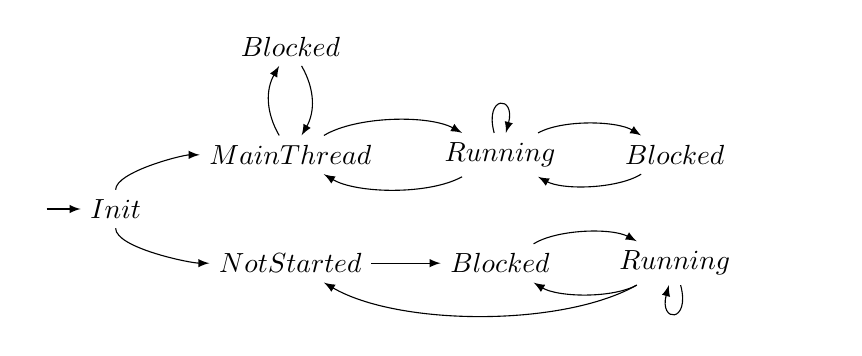
\begin{tikzpicture}
    \node at (9cm,0) (width) {};
    \node at (0,1.5cm) (height) {};

    \path (0,0) --
    node[pos=0.00] (Initxpos) {}
    node[pos=0.25] (Interpreterxpos) {}
    node[pos=0.55] (Executexpos) {}
    node[pos=0.8] (ExecuteAndPollxpos) {}
    (width);

    \path (0,0) --
    node[pos=0] (threadypos) {}
    node[pos=0.5] (Initypos) {}
    node[pos=1] (mainypos) {}
    node[pos=2] (mainBlockedypos) {}
    (height);

    \path (Initxpos |- Initypos) node (Init) {$Init$} ++(-1cm,0cm) node (start) {};
    \node at (Interpreterxpos |- mainypos) (IMn) {$MainThread$};
    \node at (Executexpos |- mainypos) (MRn) {$Running$};
    \node at (Interpreterxpos |- mainBlockedypos) (MBl) {$Blocked$};
    \node at (ExecuteAndPollxpos |- mainypos) (MB2) {$Blocked$};
    \node at (Interpreterxpos |- threadypos) (NSt) {$NotStarted$};
    \node at (Executexpos |- threadypos) (TBl) {$Blocked$};
    \node at (ExecuteAndPollxpos |- threadypos) (TRn) {$Running$};

    \draw[-latex] (start) to (Init);
    \draw[-latex] (Init) to[out=90,in=180,looseness=0.5] (IMn);
    \draw[-latex] (Init) to[out=270,in=180,looseness=0.5] (NSt);
    \draw[-latex] (IMn) to[bend left,looseness=0.7] (MRn);
    \draw[-latex] (MRn) to[bend left,looseness=0.7] (IMn);
    \draw[-latex] (MRn) to[bend left,looseness=0.7] (MB2);
    \draw[-latex] (MB2) to[bend left,looseness=0.7] (MRn);
    \draw[-latex] (IMn) to[bend left,looseness=1.0] (MBl);
    \draw[-latex] (MBl) to[bend left,looseness=1.0] (IMn);
    \draw[-latex] (NSt) to (TBl);
    \draw[-latex] (TBl) to[bend left,looseness=0.7] (TRn);
    \draw[-latex] (TRn) to[bend left,looseness=0.7] (TBl);
    \draw[-latex] (TRn) to[bend left,looseness=0.7] (NSt);
    \draw[-latex] (TRn) to[loop below] (TRn);
    \draw[-latex] (MRn) to[loop above] (MRn);
  \end{tikzpicture}
  \caption{The overall control flow of $Thr$}
  \label{interpreter-flow-figure}
\end{figure}


The $MainThread$ action is shown below.
It begins by accepting a $StackID$ from the $Launcher$ on the
$initMainThread$ channel, which is used to initialise the
$frameStackID$ state component.
It then offers a choice of executing a method on the $main$ thread in
response to a request from the $Launcher$, or switching to another
thread.
A request to start execution of a method is handled in the
$StartIntepreter$ action, which creates the $StackFrame$ for the
method.
The process then behaves as the $Running$ action, executing bytecode
instructions until the method has finished, after which the
$MainThread$ action recurses to offer the choice of method execution
and thread switch again.
If an instruction to switch to another thread from the scheduler is
received on the $CEEswitchThread$ channel, then it is only accepted if
the thread switched from is the $thread$ represented by the process.
If it is accepted, then the process behaves as $Blocked$, waiting for
a request to switch back to the thread, after which it recurses back
to offer the choice of behaviours again.
\begin{circusaction}
  MainThread \circdef initMainThread?stack \then frameStackID := Initialised~stack \circseq \circmu X \circspot \\
  \t1 \circblockbegin
  StartInterpreter \circseq Running \circseq X \\
  {} \extchoice {} \\
  CEEswitchThread?from?to \prefixcolon (from = thread) \then Blocked \circseq X
  \circblockend
\end{circusaction}

The $StartIntepreter$ action, used by $MainThread$ also handles
special methods that execute nested methods.
Its definition is shown below.
It accepts communication on the $executeMethod$ channel, requiring the
$ThreadID$ communicated to be the same as that of the current thread,
$thread$, and storing the other values communicated as $classID$,
$methodID$ and $methodArgs$.
A data operation $ResolveMethod$ is then used to determine the
appropriate class information for the method, since the method may
actually be defined in a superclass of the provided $classID$.
$ResolveMethod$ follows the method resolution rules of the JVM
specification, first checking if the class corresponding to $classID$
defines the method, then checking if one of its superclasses defines
the method, and finally looking for the method definition among its
superinterfaces.
The $Class$ information resulting from this is stored in $class$ and
used to create a new $StackFrame$ on the $frameStack$ in
$InterpreterNewStackFrame$.
The $baseFrame$ value for this stack frame is set to $\true$, since it
is being created in reponse to an external request.
\begin{circusaction}
  StartInterpreter \circdef \\
  \t1  \circvar classID : ClassID; methodID : MethodID; methodArgs : \seq Word; class : Class \circspot \\
  \t1 executeMethod?t \prefixcolon (t = thread) ?c?m?a \then classID, methodID, methodArgs := c, m, a \circseq \\
  \t1 \lschexpract ResolveMethod[cs/cs?] \rschexpract \circseq \lschexpract \exists baseFrame? == \true @ InterpreterNewStackFrame \rschexpract
\end{circusaction}

For threads other than $main$, the behaviour is described by the
$NotStarted$ action below.
It accepts a request to start the $thread$ represented by the process
from the scheduler on the $CEEstartThread$ channel.
The identifier, $bsid$, of the thread's backing store is then passed
to $ObjMan$ via the $addThreadMemory$ channel and the $stack$
identifier is used to initialise $frameStackID$.
The remaining information is stored in $classID$, $methodID$ and
$methodArgs$, and the $Class$ information is determined and a new
$StackFrame$ is created, similarly to what happends in
$StartInterpreter$. 
The process then behaves as the $Blocked$ action, waiting for an
instruction to switch to that thread, after which it behaves as the
$Running$ action, executing bytecode instructions.
When the execution of the thread's method has finished, the scheduler
is signalled on the $CEEremoveThread$ channel.
This causes the scheduler to switch to a different thread, so a thread
switch is accepted on the $CEEswitchThread$ channel.
After that, the action recurses to allow the thread to be restarted.
\begin{circusaction}
  NotStarted \circdef \\
  \t1 \circvar classID : ClassID; methodID : MethodID; methodArgs : \seq Word; class : Class \circspot \\
  \t1 CEEstartThread?toStart?bsid?stack?cid?mid?args \prefixcolon (toStart = thread) \then {} \\
  \t1 addThreadMemory!thread!bsid \then {} \\
  \t1 frameStackID, classID, methodID, methodArgs := Initialised~stack, cid, mid, args \circseq \\
  \t1 \lschexpract ResolveMethod[cs/cs?] \rschexpract \circseq \lschexpract \exists baseFrame? == \true @ InterpreterNewStackFrame \rschexpract \circseq \\
  \t1 Blocked \circseq Running \circseq CEEremoveThread!thread \then {} \\
  \t1 CEEswitchThread?from?to \prefixcolon (from = thread) \then NotStarted
\end{circusaction}

The $Blocked$ and $Running$ actions define the behaviour of threads
after they have been started.
The $Blocked$ action simply waits for a signal on the
$CEEswitchThread$ channel to switch to $thread$, after which it
terminates to allow execution in a different action to continue.
\begin{circusaction}
  Blocked \circdef CEEswitchThread?from?to \prefixcolon (to = thread) \then \Skip
\end{circusaction}

The $Running$ action, shown below, executes the bytecode instructions
of a program. 
It has the form of a loop that repeatedly executes until $frameStack$
is empty.
Within the loop, it handles the bytecode instruction at the current
$pc$ value in $HandleInstruction$ and then it polls for thread
switches in $Poll$.
\begin{circusaction}
  Running \circdef \\
  \t1 \circif frameStack = \emptyset \circthen \Skip \\
  \t1 {} \circelse frameStack \neq \emptyset \circthen HandleInstruction \circseq Poll \circseq Running \\
  \t1 \circfi
\end{circusaction}
The behaviour of polling for thread switches in $Poll$ permits thread
switches inbetween bytecode instructions.
Implementations that allow thread switches at other points are valid
if they retain the same sequence of externally visible events, meaning
only instructions involving communication with other parts of the
model need be atomic.
$Poll$ simply offers communication from the scheduler on the
$CEEswitchThread$ and $CEEproceed$ channels, switching to $Blocked$
upon receiving a signal on $CEEswitchThread$, and terminating on
receiving a signal on $CEEproceed$.

The $HandleInstruction$ action, shown in part below, offers a choice
of actions for handling the bytecode instructions.
There is one action for each of the instructions, with the action's
name formed from the bytecode mnemonic prefixed with $Handle$ (e.g.\
$HandleAload$ for the \texttt{aload} instruction).
\begin{circusaction}
	HandleInstruction \circdef \\
	\t1 HandleAconst\_null \extchoice HandleDup \extchoice HandleAload \extchoice HandleAstore \extchoice HandleIadd \extchoice {} \cdots
\end{circusaction}

The $Handle$ actions define the semantics for the instructions and, as
such are involved in the compilation strategy.
Many of these actions for handling bytecode instructions have a
similar form.

\subsubsection*{Bytecode Semantics}

The simplest $Handle$ actions consist of a guard requiring the $bc$
value at the current $pc$ to be a particular bytecode instruction,
followed by a data operation specified by a Z schema updating
$InterpreterState$.
This is illustrated in the definition of $HandleAconst\_null$ below,
which uses the $InterpreterAconst\_null$ schema.
\begin{circusaction}
  HandleAconst\_null \circdef \lcircguard bc~pc = aconst\_null \rcircguard \circguard \lschexpract InterpreterAconst\_null \rschexpract
\end{circusaction}
The \Circus{} actions and Z schemas for each bytecode instruction are
listed in Table~\ref{bytecode-model-table}.
We omit the definitions of the Z schemas in our description here.
Their contents are in line with the state updates for the bytecode
instructions presented in Table~\ref{bytecode-subset-table}.

\begin{table}[ht]
  \centering
  \begin{tabular}{llp{5cm}}
    \hline
    Bytecode instruction & \Circus{} action & Z schema \\
    \hline
    \texttt{aconst\_null} & $HandleAconst\_null$ & $InterpreterAconst\_null$ \\
    \texttt{aload} & $HandleAload$ & $InterpreterAload$ \\
    \texttt{areturn} & $HandleAreturn$ & $InterpreterAreturn$ \\
    \texttt{astore} & $HandleAstore$ & $InterpreterAstore$ \\
    \texttt{dup} & $HandleDup$ & $InterpreterDup$ \\
    \texttt{getfield} & $HandleGetfield$  & $InterpreterPush$ \\
    \texttt{getstatic} & $HandleGetstatic$ & $InterpreterPush$ \\
    \texttt{goto} & $HandleGoto$ & $InterpreterGoto$ \\
    \texttt{iadd} & $HandleIadd$ & $InterpreterIadd$ \\
    \texttt{iconst} & $HandleIconst$ & $InterpreterPush$ \\
    \texttt{if\_icmple} & $HandleIf\_icmple$ & $InterpreterIf\_icmple$ \\
    \texttt{ineg} & $HandleIneg$ & $InterpreterIneg$ \\
    \texttt{invokespecial} & $HandleInvokespecial$ & $InterpreterStackFrameInvoke$, $InterpreterNewStackFrame$ \\
    \texttt{invokestatic} & $HandleInvokestatic$ & $InterpreterStackFrameInvoke$, $InterpreterNewStackFrame$ \\
    \texttt{invokevirtual} & $HandleInvokevirtual$ & $InterpreterStackFrameInvoke$, $InterpreterNewStackFrame$ \\
    \texttt{new} & $HandleNew$ & $InterpreterPush$ \\
    \texttt{putfield} & $HandlePutfield$ & $InterpreterPop2$ \\
    \texttt{putstatic} & $HandlePutstatic$ & $InterpreterPop$ \\
    \texttt{return} & $HandleReturn$ & $InterpreterReturn$ \\
    \hline
  \end{tabular}
  \caption{The relationship between the bytecode instructions in our
    subset and the \Circus{} actions and Z schemas defining them}
  \label{bytecode-model-table}
\end{table}

The $HandleDup$, $HandleIadd$ and $HandleIneg$ actions follow the
simple form exemplified above.
Some instructions have parameters that must be extracted so that they
can be passed to the data operation for the instruction.
This can be seen in the definition of the $HandleAload$ action, shown
below, in which the inverse of the $aload$ constructor is used to
extract its parameter into a $variableIndex$ variable that is used by
the $IntepreterAload$ schema.
\begin{circusaction}
  HandleAload \circdef  \lcircguard bc~pc \in \ran aload \rcircguard \circguard \\
  \t1 \circvar variableIndex : \nat \circspot variableIndex := (aload\inv)~(bc~pc) \circseq \lschexpract InterpreterAload \rschexpract
\end{circusaction}
The $HandleAstore$, $HandleGoto$, $HandleIconst$ and
$HandleIf\_icmple$ actions all follow a similar form, extracting the
parameter of the bytecode instruction into a separate variable.

The actions to handle the return instructions (\texttt{areturn} and
\texttt{return}) require additional communication to pass the return
value to the $Launcher$ when returning from a method that has been
started by the $Launcher$.
This is performed by an additional action, $CheckLauncherReturn$, that
is called after return from the schema action.
This can be seen in the definition of $HandleAreturn$ below, where
$CheckLauncherReturn$ is passed the two output values from the
$InterpreterAreturn$ function.
The first output, $returnValue$, holds the return value for the
returning method, while the second, $fromBaseFrame$, is a boolean
value indicating if the $StackFrame$ for the method had its
$baseFrame$ value set to $\true$.
\begin{circusaction}
  HandleAreturn \circdef \circvar returnValue : Word; fromBaseFrame : \boolean \circspot \\
  \t1 \lcircguard bc~pc = areturn \rcircguard \circguard \lschexpract InterpreterAreturn \rschexpract \circseq \\
  \t1 CheckLauncherReturn(returnValue, fromBaseFrame)
\end{circusaction}
The form of the $HandleReturn$ action is similar, but since
$InterpreterReturn$ does not output a return value, $returnValue$
takes an arbitrary value.

Within the $CheckLauncherReturn$ action, the definition of which is
shown below, the boolean value $fromBaseFrame$ is used to determine
whether the return value should be communicated to the $Launcher$.
If $fromBaseFrame$ is set to $\true$, then that normally indicates
that the return value needs to be passed to the launcher.
The exception to this is if the return is from the first frame of a
$thread$ other than $main$, which is created in response to a
$CEEstartThread$ signal from the scheduler and so does not require a
return value to be sent to the launcher.
Thus, the condition checked is that $fromBaseFrame$ is $\true$, and
either $frameStack$ is empty or the current $thread$ is $main$.
If that is true, then $returnValue$ is sent to the $Launcher$ on the
$executeMethodRet$ channel and a signal is awaited on the
$continueExecution$ channel before continuing.
If the condition is not true then the action terminates.
\begin{circusaction}
  CheckLauncherReturn \circdef \circval returnValue : Word; \circval fromBaseFrame : \boolean \circspot \\
  \t1 \circif fromBaseFrame = \true \land (frameStack \neq \emptyset \lor thread = main) \circthen \\
  \t2 executeMethodRet!thread!returnValue \then continueExecution?t \prefixcolon (t = thread) \then \Skip \\
  \t1 {} \circelse fromBaseFrame = \false \lor (frameStack = \emptyset \land thread \neq main) \circthen \Skip \\
  \t1 \circfi
\end{circusaction}

For the instructions that create objects and access their fields
(\texttt{new}, \texttt{getfield}, \texttt{putfield},
\texttt{getstatic} and \texttt{putstatic}), communication with
$ObjMan$ is needed.
This can be seen in the definition of $HandleGetfield$, shown below,
where the object identifier, $oid$, is popped from the $operandStack$
of the current $StackFrame$ using the data operation $IntepreterPop$,
and the field identifier is extracted from the parameter to the
bytecode instruction.
Note that $pc$ is hidden from the $InterpreterPop$, since this action
uses two data operations promoted from $StackFrame$ operations and
only one of them need update $pc$. 
This information is passed to $ObjMan$ via the $getField$ channel,
which then handles the operation.
The field's value is returned via the $getFieldRet$ channel and pushed
onto the $operandStack$ of the current $StackFrame$ by the data
operation $InterpreterPush$.
\begin{circusaction}
  HandleGetfield \circdef \lcircguard bc~pc \in \ran getfield \land (getfield\inv)~(bc~pc) \in fieldRefIndices~currentClass \rcircguard \circguard \\
  \t1 \circvar oid : ObjectID \circspot \lschexpract InterpreterPop[oid!/value!] \hide (pc, pc') \rschexpract \circseq \\
  \t1 getField!oid!(fieldOf~currentClass~((getfield\inv)~(bc~pc))) \\
  \t1 {} \then getFieldRet?value \then \lschexpract InterpreterPush \rschexpract
\end{circusaction}
The $HandleNew$, $HandlePutfield$, $HandleGetstatic$ and
$HandlePutstatic$ actions are similar, getting information from the
$operandStack$ using $InterpreterPop$, communicating with $ObjMan$ to
handle the instruction, and using $InterpreterPush$ to push returned
information onto the $operandStack$.

Finally, the method invocation instructions (\texttt{invokespecial},
\texttt{invokestatic} and \texttt{invokevirtual}), require special
handling by the virtual machine.
Since the different method invocation instructions differ only in how
the class for the method is determined and whether a \texttt{this}
object identifier is passed among the method's arguments, the
invocation of the method after this has been determined is handled by
a common $Invoke$ action.
This can be seen in the definition of the $HandleInvokespecial$ action
below.
The method identifier $mid$ is extracted from the instruction's
parameter, and the data operation $InterpreterStackFrameInvoke$ is
used to store the return $pc$ address and pop the arguments of the
method in $poppedArgs$.
The number of arguments popped, $argsToPop?$, is the $methodArguments$
value for $mid$, plus one for the \texttt{this} identifier passed to
the method.
The class identifier is then extracted from the instruction's
parameter and passed into $Invoke$ along with $mid$ and $poppedArgs$.
\begin{circusaction}
  HandleInvokespecial \circdef \circvar cid : ClassID; mid : MethodID; poppedArgs : \seq Word \circspot \\
  \t1 \lcircguard bc~pc \in \ran invokespecial \land ((invokespecial\inv)~(bc~pc)) \in methodRefIndices~currentClass \rcircguard \circguard \\
  \t1 mid := methodOf~currentClass~((invokespecial\inv)~(bc~pc)) \circseq \\
  \t1 \lschexpract \exists argsToPop? == methodArguments~mid + 1 @ InterpreterStackFrameInvoke \rschexpract \circseq \\
  \t1 Invoke(classOf~currentClass~((invokespecial\inv)~(bc~pc)), mid, poppedArgs)
\end{circusaction}
The $HandleInvokestatic$ and $HandleInvokevirtual$ actions are
similar, except that $argsToPop?$ does not include the extra
\texttt{this} argument in $HandleInvokeStatic$, and
$HandleInvokevirtual$ obtains the class identifier from the
\texttt{this} identifier via the $getClassIDOf$ channel rather than
from the instruction's parameter.

The $Invoke$ action, shown in part below, has the form of an external
choice over actions for each of the special methods supported by the
SCJVM, plus an $InvokeOther$ action for handling non-special methods
implemented in bytecode.
The name of the action for each special method is formed from the name
of the special method prefixed with $Invoke$ (e.g. 
$InvokeResumeThread$ for the \texttt{resumeThread()} method).
The parameters passed to the $Invoke$ action, which are the class
identifier, $classID$, the method identifier, $method$, and the
method argument list, $args$, are passed on to each of the actions in
the external choice.
\begin{circusaction}
  Invoke \circdef \circval classID : ClassID; \circval method : MethodID; \circval args : \seq Word \circspot \\
  \t1 InvokeResumeThread(classID, method, args) \extchoice InvokeSuspend(classID, method) \extchoice \cdots \\
  \t1 {} \extchoice InvokeOther(classID, method, args)
\end{circusaction}

Within the special method actions, there is a guard ensuring the
action is taken when the class and method identifiers are those for
the method.
The method is then handled by communication on the appropriate
channels.
This is illustrated by the definition of the $InvokeResumeThread$
action, shown below.
The class identifier parameter, $classID$, is required to refer to a
subclass of some class $resumeThreadClass$, while the method
identifier, $method$, must be $resumeThreadID$.
The class and method identifiers used in the special method actions
are a mixture of identifiers from the SCJ API and
implementation-defined identifiers provided to expose SCJVM services
to bytecode programs.
The argument to the method, stored as the first element of the
$methodArgs$ parameter, is converted to a $ThreadID$ and passed to the
$Launcher$ via the $resumeThread$ channel.
A return signal is then awaited on the $resumeThreadRet$ channel
before continuing.
\begin{circusaction}
  InvokeResumeThread \circdef \\
  \t1 \circval classID : ClassID; \circval method : MethodID; \circval methodArgs : \seq Word \circspot \\
  \t1 \lcircguard (classID,resumeThreadClass) \in subclassRel~cs \land method = resumeThreadID \rcircguard \circguard {} \\
  \t1 resumeThread!(WordToThreadID~(methodArgs~1)) \then resumeThreadRet \then \Skip
\end{circusaction}

Some of the special methods start other methods as part of their
execution, which requires additional handling.
An example is \texttt{enterPrivateMemory()} from the SCJ API, which
executes the \texttt{run()} method of a \texttt{Runnable} object after
entering a private memory area.
This is handled in the action $InvokeEnterPrivateMemory$, shown below.
It begins in a similar way to $InvokeResumeThread$, with a guard on
the $classID$ and $method$ passed into the action.
The method is then handled by communicating with the $Launcher$ on the
$enterPrivateMemory$ channel, passing the arguments from $methodArgs$.
The execution of the nested method is then handled as in
$StartInterpreter$, waiting for the request to execute the nested
method on the $executeMethod$ channel and creating a new $StackFrame$
for it.
\begin{circusaction}
  InvokeEnterPrivateMemory \circdef \\
  \t1 \circval classID : ClassID; \circval method : MethodID; \circval methodArgs : \seq Word \circspot \\
  \t1 \lcircguard (classID,managedMemoryClass) \in subclassRel~cs \land method = enterPrivateMemoryID \rcircguard \circguard {} \\
  \t2 enterPrivateMemory!thread!(methodArgs~1)!(methodArgs~2) \then StartInterpreter
\end{circusaction}

In addition to the special methods handled in the $Launcher$, we also
supply \texttt{read()} and \texttt{write()} methods for reading from
and writing to some standard input and output device. 
These methods are handled using the \texttt{input} and \texttt{output}
channels that communicate the values from and to the environment of
the SCJVM.
This is shown in the definition of the $InvokeRead$ action below,
which accepts the input on the $input$ channel and pushes it onto the
stack as the return value for the method.
\begin{circusaction}
  InvokeRead \circdef \\
  \t1 \circval classID : ClassID; \circval method : MethodID; \circval methodArgs : \seq Word \circspot \\
  \t1 \lcircguard (classID,readClass) \in subclassRel~cs \land method = readID \rcircguard \circguard {} \\
  \t2 input?value \then \lschexpract InterpreterPush \hide (pc,pc') \rschexpract
\end{circusaction}
The $InvokeWrite$ action is similar, writing the method argument to
the $output$ channel.

The $InvokeOther$ action, shown in part below, describes the handling
of non-special methods.
It begins with a guard that is the conjunction of the negation of the
guards for the invocation actions for the special methods.
The actions starts execution of the method in the interpreter by
finding its $Class$ information with $ResolveMethod$ and creating a
new $StackFrame$ with $IntepreterNewStackFrame$.
The $baseFrame$ value is set to $\false$ here, since the stack frame
is created due to execution of a bytecode instruction in the
interpreter, rather than in response to an external request.
\begin{circusaction}
  InvokeOther \circdef \circval classID : ClassID; \circval methodID : MethodID; \circval methodArgs : \seq Word \circspot \\
  \t1 \lcircguard ((classID,resumeThreadClass) \notin subclassRel~cs \lor methodID \neq resumeThreadID) \\
  \t2 {} \land \cdots \\
  \t2 {} \land ((classID, writeClass) \notin subclassRel~cs \lor methodID \neq writeID) \rcircguard \circguard {} \\
  \t1 \circvar class : Class \circspot \\
  \t1 \lschexpract ResolveMethod[cs/cs?] \rschexpract \circseq \lschexpract \exists baseFrame? == \false @ InterpreterNewStackFrame \rschexpract
\end{circusaction}

This concludes our description of the handling of bytecode
instructions, and of our description of the CEE before the application
of the compilation strategy.
In the next section we describe the model of the C code that is used
for the output of the compilation strategy.

\section{C Code Model}
\label{cee-c-code-section}

As mentioned previously, the CEE after compilation to C has a similar
structure to the CEE before compilation, but the object manager is
replaced with a struct manager and the intepreter is replaced with the
C program.
The struct manager is represented by a process $StructMan_{cs}$, and
the C program by a process $CProg_{bc,cs}$.
These are place in parallel composition with the $Launcher$ process
described in Section~\ref{cee-launcher-section} to form a $CCEE_{bc,cs}$
process representing the CEE for a C program, as shown below.
\begin{circus}
  CEE_{bc,cs}(sid, initOrder) \circdef StructMan_{cs} \parallel CProg_{bc,cs} \parallel Launcher(sid, initOrder)
\end{circus}
The subscripts here indicate that the processes depend on the $bc$ and
$cs$ constants used as inputs to the compilation strategy. 
However, $bc$ and $cs$ are not true parameters of the processes and so
are not referenced within the processes.
Note that the $sid$ and $initOrder$ parameters to $Launcher$ remain as
parameters here since $Launcher$ is not transformed during the
compilation strategy.

The channels used for communication between these processes are the
same as those in Table~\ref{cee-channel-table}, except that the
$getField$, $getFieldRet$ and $putField$ channels are replaced with
$getObject$, $getObjectRet$ and $putObject$ channels.
The new channels are discussed in more detail in the
Section~\ref{cee-struct-manager-subsection}, which describes the
struct manager.
After that, in Section~\ref{cee-c-program-subsection}, the
$CProg_{bc,cs}$ process is described and the shallow embedding of C it
uses is discussed.

\subsection{Struct Manager}
\label{cee-struct-manager-subsection}

$StructMan_{cs}$ manages objects represented by C structs that
incorporate the class information from $cs$, refining the process
$ObjMan$, which handles abstract objects.
$StructMan_{cs}$ has Z schemas representing struct types for objects
of each class.
For each class identifier ${<}classID_1{>}, \dots, {<}classID_n{>}$,
we define a schema ${<}classID_k{>}Obj$ for $k \in \{1,\dots,n\}$,
representing the objects of that class. 
They begin with a $classID$ component containing the class identifier
of the object, so that polymorphic method calls can be made by choice
over the object's class.
There is then a component for each of the fields
${<}fieldID_1{>}, \dots, {<}fieldID_{m_k}{>}$ of the class, with each
component having the type $Word$.
\begin{schema}{{<}classID_k{>}Obj}
  classID : ClassID \\
  {{<}fieldID_{k,1}{>}} : Word \\
  \t1 \vdots \\
  {{<}fieldID_{k,m_k}{>}} : Word
\end{schema}

The schema types for each type of object are combined into a single
free type $ObjectStruct$.
The constructor for each ${<}classID_k{>}$ is called
${<}classID_k{>}Con$, with a single parameter of type
${<}classID_k{>}Obj$.
\begin{zed}
  ObjectStruct ::= {<}classID_1{>}Con \ldata {<}classID_1{>}Obj \rdata | \dots | {<}classID_n{>}Con \ldata {<}classID_n{>}Obj \rdata
\end{zed}

For each object type, we define a natural number constant
$sizeof{<}classID_k{>}Obj$ that represents the result of applying C's
\texttt{sizeof} operator to the struct represented by the
corresponding ${<}classID_k{>}Obj$ type.
We also define a function $classIDOf$ for obtaining the value of the
common $classID$ field from an $ObjectStruct$ value.
Additionally, we define a $cast{<}classID_k{>}$ function for each
${<}classID_k{>}$, which maps an $ObjectStruct$ value to a
${<}classID_k{>}Obj$ value.
This works not only for values in the range of the
${<}classID_k{>}Con$ constructor, but also for any class that is a
subclass of ${<}classID_k{>}$, with the common fields copied across.
Thus, $cast{<}classID_k{>}$ represents casting of C structs, where a
struct can be truncated by casting to a struct whose fields are a
prefix of it.
Finally, we also define a function
$update{<}classID_k{>}\_{<}fieldID{>}_i$ for each class identifier
${<}classID_k{>}$ and field identifier ${<}fieldID_i{>}$, which takes
an $ObjectStruct$ and updates the specified field with a given value.
This represents a combined cast and update.

Channels $getObject$, $getObjectRet$, and $putObject$, the definitions
of which are shown below, are used to pass $ObjectStruct$ values to
and from $StructMan_{cs}$.
\begin{circus}
  \circchannel getObject : ObjectID \\
  \circchannel getObjectRet : ObjectStruct \\
  \circchannel putObject : ObjectID \cross  ObjectStruct
\end{circus}

For the static class fields, the static fields from each class
${<}classID_1{>}, \dots, {<}classID_n{>}$ are collected together in a
schema $StaticFields$, as shown below.
\begin{schema}{StaticFields}
  {<}classID_1{>}\_{<}staticfieldID_{1,1}{>} : Word \\
  \t1 \vdots \\
  {<}classID_1{>}\_{<}staticfieldID_{1,\ell_1}{>} : Word \\
  \t1 \vdots \\
  {<}classID_n{>}\_{<}staticfieldID_{n,1}{>} : Word \\
  \t1 \vdots \\
  {<}classID_n{>}\_{<}staticfieldID_{n,\ell_n}{>} : Word
\end{schema}
We define a natural number constant $sizeofStaticFields$ giving the
amount of space required for the struct represented by $StaticFields$.

The $StaticFields$ type is communicated using the $getStaticFields$
and $putStaticFields$ channels, the definitions of which are shown
below.
\begin{circus}
  \circchannel getStaticFields : StaticFields \\
  \circchannel putStaticFields : StaticFields
\end{circus}

The state of $StructMan_{cs}$ is given by the schema $StructManState$,
shown below.
This is similar to $ObjManState$, but the $objects$ map relates object
identifiers to $ObjectStruct$ values, and $staticClassFields$ is a map
from $ObjectID$ to the $StaticFields$ type.
We omit the invariant as it is similar to the invariant of
$ObjManState$.
\begin{schema}{StructManState}
  objects : ObjectID \pfun ObjectStruct \\
  backingStoreMap : BackingStoreID \pfun \finset ObjectID \\
  backingStoreStacks : ThreadID \pfun \seq_1 BackingStoreID \\
  rootBS : BackingStoreID \\
  staticClassFieldsID : StaticFieldsStructID \\
  staticClassFields : ObjectID \pfun StaticFields
\where
  \dots
\end{schema}

Within the $StructMan_{cs}$ process, the structure is much the same as
for the $ObjMan$ process, with the state initialised in the same way.
However, $AllocateStaticFields$ is changed to handle the
$StaticFields$ type.
The definition of $AllocateStaticFields$ in $StructMan_{cs}$ is as
shown below.
It is similar to the $ObjMan$ definition of $AllocateStaticFields$,
but it does not collect the required field identifiers since that is
already implicitly done in the definition of $StaticFields$.
The required size for the allocated space is now $sizeofStaticFields$.
The initialisation of the static fields, in $InitStaticFields$ is much
the same, but now specialised to refer to $StaticFields$, setting all
its components to $null$.
\begin{circusaction}
  AllocateStaticFields \circdef \\
  \t1 MMallocateMemory!(last~(backingStoreStacks~main))!(sizeofStaticFields) \then {} \\
  \t1 MMallocateMemoryRet?objectID \then {} \\
  \t2 (MMreport?r \prefixcolon (r = MMokay) \then \lschexpract InitStaticFields \rschexpract \\
  \t2 {} \extchoice MMreport?r \prefixcolon (r = MMokay) \then \Chaos)
\end{circusaction}

Also, the actions $GetField$, $PutField$, $GetStatic$ and $PutStatic$
are replaced with new actions $GetObject$, $PutObject$, $GetStaticFields$ and
$PutStaticFields$.
These are fairly simple, with $GetObject$ and $PutObject$ retrieving
and storing $ObjectStruct$ values in the $objects$ map.
These are presented exposed on the $getObject$ and $getObjectRet$
channels for $GetObject$, and the $putObject$ channel for $PutObject$. 
Similarly, $GetStaticFields$ and $PutStaticFields$ retrieve and store
the $StaticFields$ value associated with $staticClassFieldsID$ from
the $staticClassFields$ map.
These are performed on the $getStaticFields$ and $putStaticFields$
channels respectively.
We omit the definitions of these actions here; their definitions are
given in Appendix~\ref{struct-manager-appendix}, which shows the
general form of the $StructMan_{cs}$ process.

The $NewObject$ action is different in $StructMan_{cs}$ to that in
$ObjMan$. 
It uses the same channels ($newObject$ and $newObjectRet$), but must
create the correct $ObjectStruct$ value for the provided class.
It has the form shown below.
The $thread$ and $classID$ identifiers are received from the
$newObject$ channel, and a choice is then made over the $classID$,
matching it against each class identifier supported by
$StructMan_{cs}$.
If $classID$ matches a class identifier ${<}classID_k{>}$, then space
for the object is allocated via communication with the memory manager,
as in $AllocateStaticFields$, then the object is stored in $objects$
and initialised.
The allocation is performed in a separate action, $AllocateObject$, as
it is similar for each class.
The size of the object is given by the $sizeof{<}classID_k{>}$
identifier for ${<}classID_k{>}$, and the returned object identifier
is stored in $objectID$.
The storing and initialisation of the object is then done in a schema
action $StructMan{<}classID_k{>}ObjInit$, which sets all the object's
fields to $null$ and puts it in $objects$, stored within
${<}classID_k{>}Con$. 
Finally, $objectID$ is returned via the $newObjectRet$ channel.
\begin{circusaction}
  NewObject \circdef \circvar objectID : ObjectID \circspot \\
  \t1 newObject?thread?classID \then \\
  \t1 \circif classID = {{<}classID_1{>}} \circthen {} \\
  \t2 AllocateObject(thread, sizeof{<}classID_1{>}, objectID) \circseq \lschexpract StructMan{<}classID_1{>}ObjInit \rschexpract \\
  \t1 {} \circelse classID = {{<}classID_2{>}} \circthen {} \\
  \t2 AllocateObject(thread, sizeof{<}classID_2{>}, objectID) \circseq \lschexpract StructMan{<}classID_2{>}ObjInit \rschexpract \\
  \t2 \vdots \\
  \t1 {} \circelse classID = {{<}classID_n{>}} \circthen {} \\
  \t2 AllocateObject(thread, sizeof{<}classID_n{>}, objectID) \circseq \lschexpract StructMan{<}classID_n{>}ObjInit \rschexpract \\
  \t1 \circfi \circseq newObjectRet!objectID \then \Skip \\
\end{circusaction}

Finally, $GetClassIDOf$ is changed to extract the class identifier
from an $ObjectStruct$ value using the $classIDOf$ function.
This is not used in the C code, which, as we will see in the next
section, uses $classIDOf$ directly, but is supplied for use by the
$Launcher$, which is unchanged by the strategy.
We omit the definition of $GetClassIDOf$ here.

In the next section we describe the structure of the C code of the
program and our shallow embedding of C in \Circus{}, which makes use
of some of the types and channels discussed in this section.

\subsection{Shallow Embedding of C in \Circus{}}
\label{cee-c-program-subsection}

The C code output by our compilation strategy is represented by a
\Circus{} process $CProg_{bc,cs}$, which is determined by the bytecode
instructions, $bc$, and the class information, $cs$.
This process has a similar structure to that of $Interpreter$:~a
parallel composition of $CThr_{bc,cs}(t)$ processes representing C
threads, one for each thread identifier $t$ except the $idle$ thread,
as shown in the definiton of $CProg_{bc,cs}$ below.
\begin{circus}
  \circprocess CProg_{bc,cs} \circdef \Parallel t : ThreadID \setminus \{ idle \} \lpar ThrChans(t) \rpar \circspot CThr_{bc,cs}(t)
\end{circus}

The $CThr_{bc,cs}$ process has a similar structure to the $Thr$
process presented in Section~\ref{cee-interpreter-subsection}.
However, the $pc$ and $frameStack$ components are eliminated from the
state during compilation.
Thus, the state of $CThr_{bc,cs}$, shown in $CThrState$ below, just
contains $stackID$, which has the same type as $frameStackID$ in
$InterpreterState$ and so may be $Uninitialised$ or $Initialised$ with
a $StackID$ for the C thread's stack.
Since there is no explicit stack in C, we only need to ensure there is
a stack identifier in $stackID$ so space for the thread's stack has
been allocated and the $stackID$ is not manipulated beyond that.
\begin{schema}{CThrState}
  stackID : Stack
\end{schema}
The $stackID$ is initially set to $Uninitialised$.

The $Running$ action and creation of stack frames are also replaced
with an $ExecuteMethod$ action that executes the C function
corresponding to a given method identifier.
The main action of $CThr_{bc,cs}$ thus has the same structure as that
of $Interpreter$, with a choice of $MainThread$ for the $main$ thread
and $NotStarted$ for non-$main$ threads.
However, $MainThread$ now has the structure shown below.
This is similar to the definition of $MainThread$ in $Thr$, but the
information received from the $executeMethod$ channel is passed into
the $ExecuteMethod$ action to select the correct C function to
execute.
After method execution has finished, the return value, $retVal$, is
obtained from $ExecuteMethod$ and communicated on the
$executeMethodRet$ channel.
\begin{circusaction}
  MainThread \circdef initMainThread?stack \then stackID := Initialised~stack \circseq \circmu X \circspot \\
  \t1 \circblockbegin
  \circvar retVal : Word \circspot executeMethod?t \prefixcolon (t = thread) ?cid?mid?args \then {} \\
  \t1 ExecuteMethod(cid,mid,args,retVal) \circseq \\
  \t1 executeMethodRet!retVal \then continueExecution \then X \\
  {} \extchoice {} \\
  CEEswitchThread?from?to \prefixcolon (from = thread) \then Blocked
  \circseq X \circblockend
\end{circusaction}

Similarly, the $NotStarted$ action in $CThr_{bc,cs}$ has the form
shown below, with $ExecuteMethod$ after $Blocked$, replacing
$Running$.
The return value, $retVal$, is discarded here since the methods that
are executed a the top level on the non-$main$ threads should not
return a value so $retVal$ will be arbitrary.
The thread's removal is also handled by $CEEremoveThread$ so no
communication on $executeMethodRet$ follows the end of the method's
execution.
\begin{circusaction}
  NotStarted \circdef \\
  \t1 \circvar classID : ClassID; methodID : MethodID; methodArgs : \seq Word; class : Class \circspot \\
  \t1 CEEstartThread?toStart?bsid?stack?cid?mid?args \prefixcolon (toStart = thread) \then {} \\
  \t1 addThreadMemory!thread!bsid \then {} \\
  \t1 frameStackID, classID, methodID, methodArgs := Initialised~stack, cid, mid, args \circseq \\
  \t1 Blocked \circseq \circvar retVal : Word \circspot ExecuteMethod(classID, methodID, methodArgs, retVal) \circseq \\
  \t1 CEEremoveThread!thread \then CEEswitchThread?from?to \prefixcolon (from = thread) \then NotStarted
\end{circusaction}

The $ExecuteMethod$ action has the form shown below.
It takes as parameters the class identifier, $cid$, method identifier,
$mid$, and arguments list, $args$, for the method to be executed.
It then chooses the appropriate action corresponding to the supplied
$cid$ and $mid$, and passes the appropriate number of arguments from
$args$ to the action.
The return value of each of the actions, if they return one, is
captured in $retVal$ to be returned to $MainThread$ or $NotStarted$.
\begin{circusaction}
  ExecuteMethod \circdef \\
  \t1 \circval cid : ClassID; \circval mid : MethodID; \circval args : \seq Word; \circres retVal : Word \circspot \\
  \t1 \circif (cid,mid) = ({<}classID_1{>}, {<}methodID_1{>}) \circthen {} \\
  \t2 {<}classID_1{>}\_{<}methodID_1{>}(args~1,\dots,args~(methodArgs~{<}methodID_1{>}), retVal) \\
  \t2 \vdots \\
  \t1 {} \circelse (cid,mid) = ({<}classID_n{>}, {<}methodID_{m_n}{>}) \circthen {} \\
  \t2 {<}classID_n{>}\_{<}methodID_{m_n}{>}(args~1,\dots,args~(methodArgs~{<}methodID_{m_n}{>}), retVal) \\
  \t1 \circif
\end{circusaction}

The actions used by $ExecuteMethod$ represent C functions containing
the behaviour of the compiled methods.
The name of each action is made up of the class and method identifier
for the method, separated by an underscore.
Within the action, the constructs of C are represented by constructs
of \Circus{}. 
The representation of these constructs is summarised in
Table~\ref{embedding-table}.

\begin{table}[t]
\centering
{\scriptsize
\setlength{\zedindent}{0pt}
\setlength{\zedleftsep}{2mm}
\setlength{\zedtab}{1em}
\setlength{\abovedisplayskip}{0mm}
\setlength{\belowdisplayskip}{0mm}
\setlength{\abovedisplayshortskip}{0mm}
\setlength{\belowdisplayshortskip}{0mm}
\renewcommand{\arraystretch}{0.5}
\rowcolors{2}{white}{lightgray}
\begin{tabular}{p{3cm}p{5cm}p{4cm}}
\hline
Construct & C code & \Circus{} equivalent \\
\hline %%%%%%%%%%%%%%%%%%%%%%%%%%%%%%%%%%%%%%%%%%%%%%%%%%%%%%%%%%%%%%%%
\raggedright \hfill \newline Function definition &
\begin{lstlisting}
void foo() {...}
\end{lstlisting}
&
\[
Foo \circdef \cdots
\] \\
%\hline %%%%%%%%%%%%%%%%%%%%%%%%%%%%%%%%%%%%%%%%%%%%%%%%%%%%%%%%%%%%%%%%
\raggedright \hfill \newline Function definition with argument &
\begin{lstlisting}
void bar(int32_t x) {...}
\end{lstlisting}
&
\[
  Bar \circdef \circval x : Word \circspot \cdots
\] \\
%\hline %%%%%%%%%%%%%%%%%%%%%%%%%%%%%%%%%%%%%%%%%%%%%%%%%%%%%%%%%%%%%%%%
\raggedright \hfill \newline Function definition with return value &
\begin{lstlisting}
int32_t baz() {...}
\end{lstlisting}
&
\[
  Baz \circdef \circres retVal : Word \circspot \cdots
\] \\
% \hline %%%%%%%%%%%%%%%%%%%%%%%%%%%%%%%%%%%%%%%%%%%%%%%%%%%%%%%%%%%%%%%
\raggedright \hfill \newline Function definition with parameter and return value &
\begin{lstlisting}
int32_t quux(int32_t x) {...}
\end{lstlisting}
&
\[
  Quux \circdef \circval x : Word; \\
  \t1 \circres retVal : Word \circspot \cdots
\] \\
% \hline %%%%%%%%%%%%%%%%%%%%%%%%%%%%%%%%%%%%%%%%%%%%%%%%%%%%%%%%%%%%%%%
\raggedright \hfill \newline Function call &
\begin{lstlisting}
foo();
\end{lstlisting}
&
\[
Foo
\] \\
%\hline %%%%%%%%%%%%%%%%%%%%%%%%%%%%%%%%%%%%%%%%%%%%%%%%%%%%%%%%%%%%%%%%
\raggedright \hfill \newline Function call with argument &
\begin{lstlisting}
bar(x);
\end{lstlisting}
&
\[
Bar(x)
\] \\
%\hline %%%%%%%%%%%%%%%%%%%%%%%%%%%%%%%%%%%%%%%%%%%%%%%%%%%%%%%%%%%%%%%%
\raggedright \hfill \newline Function call with return value &
\begin{lstlisting}
x = baz();
\end{lstlisting}
&
\[
Baz(x)
\] \\
%\hline %%%%%%%%%%%%%%%%%%%%%%%%%%%%%%%%%%%%%%%%%%%%%%%%%%%%%%%%%%%%%%%%
\raggedright \hfill \newline Function call with argument and return value &
\begin{lstlisting}
y = quux(x);
\end{lstlisting}
&
\[
Quux(x,y)
\] \\
%\hline %%%%%%%%%%%%%%%%%%%%%%%%%%%%%%%%%%%%%%%%%%%%%%%%%%%%%%%%%%%%%%%%
\raggedright \hfill \newline Return statement &
\begin{lstlisting}
return;
\end{lstlisting}
&
\begin{circus}
\Skip
\end{circus} \\
%\hline %%%%%%%%%%%%%%%%%%%%%%%%%%%%%%%%%%%%%%%%%%%%%%%%%%%%%%%%%%%%%%%%
\raggedright \hfill \newline Return statement with value &
\begin{lstlisting}
return x;
\end{lstlisting}
&
\begin{circus}
  retVal := x
\end{circus} \\
%\hline %%%%%%%%%%%%%%%%%%%%%%%%%%%%%%%%%%%%%%%%%%%%%%%%%%%%%%%%%%%%%%%%
\raggedright \hfill \newline Assignment &
\begin{lstlisting}
x = e;
\end{lstlisting}
&
\begin{circus}
x := e
\end{circus} \\
%\hline %%%%%%%%%%%%%%%%%%%%%%%%%%%%%%%%%%%%%%%%%%%%%%%%%%%%%%%%%%%%%%%%
\raggedright \hfill \newline Variable declaration &
\begin{lstlisting}
int32_t x;
\end{lstlisting}
& \[\circvar x : Word \circspot \] \\
%\hline %%%%%%%%%%%%%%%%%%%%%%%%%%%%%%%%%%%%%%%%%%%%%%%%%%%%%%%%%%%%%%%%
\raggedright \hfill \newline Variable declaration and initialisation &
\begin{lstlisting}
int32_t x = e;
\end{lstlisting}
& \[\circvar x : Word \circspot x := e\] \\
%\hline %%%%%%%%%%%%%%%%%%%%%%%%%%%%%%%%%%%%%%%%%%%%%%%%%%%%%%%%%%%%%%%%
\raggedright \hfill \newline If statement &
\begin{lstlisting}
if (b) {...}
\end{lstlisting}
&
\[
\circif b \circthen \cdots \\
{} \circelse \lnot b \circthen \Skip \\
\circfi
\] \\
%\hline %%%%%%%%%%%%%%%%%%%%%%%%%%%%%%%%%%%%%%%%%%%%%%%%%%%%%%%%%%%%%%%%
\raggedright \hfill \newline If-else statement &
\begin{lstlisting}
if (b) {...} else {...}
\end{lstlisting}
&
\[
\circif b \circthen \cdots \\
{} \circelse \lnot b \circthen \cdots \\
\circfi
\] \\  
%\hline %%%%%%%%%%%%%%%%%%%%%%%%%%%%%%%%%%%%%%%%%%%%%%%%%%%%%%%%%%%%%%%%
\raggedright \hfill \newline Infinite loop &
\begin{lstlisting}
while (1) {...}
\end{lstlisting}
&
{
\[
\circmu X \circspot\cdots \circseq X
\]}\\
%\hline %%%%%%%%%%%%%%%%%%%%%%%%%%%%%%%%%%%%%%%%%%%%%%%%%%%%%%%%%%%%%%%%
\raggedright \hfill \newline While loop &
\begin{lstlisting}
while (b) {...}
\end{lstlisting}
&
{
\def\arraystretch{1.1}
\[
\circmu X \circspot \\
  \t1 \circif b \circthen \cdots \circseq X \\
  \t1 {} \circelse \lnot b \circthen \Skip \\
  \t1 \circfi
\]}\\  
%\hline %%%%%%%%%%%%%%%%%%%%%%%%%%%%%%%%%%%%%%%%%%%%%%%%%%%%%%%%%%%%%%%%
\raggedright \hfill \newline Do-while loop &
\begin{lstlisting}
do {...} while (b);
\end{lstlisting}
&
{
\def\arraystretch{1.1}
\[
  \circmu X \circspot \cdots \circseq \\
  \t1 \circif b \circthen X \\
  \t1 {} \circelse \lnot b \circthen \Skip \\
  \t1 \circfi
\]}\\
\hline %%%%%%%%%%%%%%%%%%%%%%%%%%%%%%%%%%%%%%%%%%%%%%%%%%%%%%%%%%%%%%%%%
\end{tabular}}
\caption{The \Circus{} representations of C constructs in our shallow
  embedding}
\label{embedding-table}
\end{table}

The constructs we allow within a C function are conditionals, while
loops, assignment statements, and function calls.
These are comparable with those allowed in MISRA-C~\cite{MISRA} and
present in the code generated by icecap.
Conditionals in C correspond to \Circus{} alternation blocks, similar
to those in Dikstra's guarded command language~\cite{dijkstra1975}.
We handle loops in C using recursion in \Circus{}, with alternation
used to handle loop conditions.

As each function in the C code is a \Circus{} action, function calls
are represented as references to those actions.
Function arguments in C are passed by value, although those values may
be pointers to other values.
Accordingly, since our SCJVM model represents pointers explicitly (via
the object/struct manager), we represent function arguments using
value parameters of the \Circus{} action.

If a function has a return value, it is represented with a result
parameter of the \Circus{} action, usually named $retVal$, with an
assignment to that parameter at the end of the action representing
return statements.
We assume there is a single return statement at the end of the
function, so the return can simply be represented by the termination
of the action if there is no return value.
It is not necessary to cater for return statements in the middle of a
function as we have control over the structure of the functions.
We follow guidelines for safety-critical uses of C variants, such as
MISRA-C~\cite{MISRA}, and use a single return statement at the end of
a function.
A function with both a return value and arguments has its value
parameters (representing the arguments) followed by the result
parameter (representing the return value).

Local variables of the function are represented using \Circus{}
variable blocks.
These are placed near the start of the action, after the parameter
declarations.
While \Circus{} variable blocks could also be used to represent
variables declared in the middle of functions, that is not necessary
for our work.
Restricting ourselves to variables at the start of functions ensures
the code or strategy generates is compatible with older versions of C.


\section{Final Considerations}
\label{cee-final-considerations-section}

In this chapter we have presented our model of the core execution
environment (CEE) of an SCJVM and specified the subset of Java
bytecode covered in our model.
Our bytecode subset consists of 14 instructions, which focus on method
invocation and the manipulation of objects, since those are core
concepts of Java.
We have omitted instructions for exception handling, since that would
complicate the model while adding little power.
Our subset is sufficiently small to permit reasoning, but large enough
to express a variety of SCJ programs.

Our CEE model is divided in three components, with a \Circus{} process
representing each component.
The first component is the memory, which manages objects and the
entering of backing stores, since the memory manager discussed in the
previous chapter has no knowledge of the structure of objects.
The second component of the CEE model is the interpreter, which
describes the semantics of each of the bytecode instructions in our
subset and provides for executing methods.
The third and final component is the interpreter, which manages the
SCJ mission model and coordinates execution.

One interesting point about our model is the handling of special
methods in the interpreter and launcher.
This is necessary for several reasons: to allow methods running in the
interpreter to access the SCJVM services defined in the previous
chapter, to allow mission setup methods to interact with the launcher,
and to permit entering of memory areas by interaction with the CEE
memory component.
The handling of special methods works by having the interpreter check
upon invocation of a method whether it requires special handling.
If it does require special handling, it is passed to the launcher to
be handled.
The launcher then performs the required handling of the method,
communicating with the SCJVM services and the memory as required.

This model forms the first part of our compilation strategy, which is
the specification of the source language.
That is mostly included in the interpreter section as the semantics of
the bytecode instructions, though handling of special methods passed
to the launcher and the representation of classes and objects must
also be considered in the compilation strategy.
There are also other possible uses for the model presented in this
chapter.
Since it is a model of an interpreting SCJVM, it could be used as a
specification for an implementation of an interpreting SCJVM.
Such an SCJVM could also incorporate the compilation strategy to
provide a choice between interpreted and complied code, as in the
icecap HVM.
Additionally, since error handling in our model is done via aborting
execution, an identification of the conditions required for the model
to be divergence-free would produce requirements that can be used for
bytecode verification.


\chapter{Compilation Strategy}
\label{strategy-chapter}

In this chapter we describe our compilation strategy for refining SCJ
bytecode to C code.
We begin in Section~\ref{compilation-overview-section} with an
overview of our compilation strategy.
Then, in Section~\ref{compilation-assumptions-section} we describe the
requirements on the source program for the compilation strategy to be
applied.
Afterwards, we describe each stage of the strategy in a separate
section.
The first stage, which we call \emph{Elimination of Program Counter},
is described in Section~\ref{elimination-of-program-counter-section}.
The second stage, called \emph{Elimination of Frame Stack}, is
described in Section~\ref{elimination-of-frame-stack-section}.
Finally, the third stage of the strategy, which is called \emph{Data
  Refinement of Objects}, is described in
Section~\ref{data-refinement-of-objects-section}.
We then show how the stages fit together to show the compilation as a
whole to be correct, in Section~\ref{main-theorem-proof-section}, and
conclude with some final considerations in
Section~\ref{compilation-final-considerations-section}.

\section{Overview}
\label{compilation-overview-section}

Our compilation strategy refines the $CEE(bc,cs,instCS,sid,initOrder)$
process defined in Section~\ref{cee-interpreter-section} to obtain the
$CCEE_{bc,cs}(sid, initOrder)$ process in
Section~\ref{cee-c-code-section}.
The overall theorem for the strategy, and, therefore, the main result
presented in this chapter, is as follows.
\begin{thm}[Compilation Strategy]\label{main-theorem}
  Given $bc$, $cs$ and $sid$, there are processes $StructMan_{cs}$ and
  $CProg_{bc,cs}$ such that,
  \setlength{\zedindent}{0.5cm}
  \begin{circus}
    CEE(bc,cs,instCS,sid,initOrder) \circrefines StructMan_{cs} \parallel
    CProg_{bc,cs} \parallel Launcher(sid, initOrder).
  \end{circus}
\end{thm}
$StructMan_{cs}$ manages objects represented by C structs that
incorporate the class information from $cs$, refining the process
$ObjMan$, which handles abstract objects.
$CProg_{bc,cs}$ refines the $Interpreter$, with the $Thr$ processes
refined into the $CThr_{bc,cs}$ processes described in
Section~\ref{cee-c-program-subsection}.
This means that the threads from SCJ are mapped onto threads in C,
since we do not dictate a particular thread switch mechanism in either
the source or target models.

The compilation strategy is split into three stages.
Each stage has a theorem describing it, for which the strategy acts as
a proof.
The proof of Theorem~\ref{main-theorem}, presented in
Section~\ref{main-theorem-proof-section}, is obtained by an
application of the theorems for each stage.
Each stage of the compilation strategy handles a different part of the
$Interpreter$ state:~the $pc$, the $frameStack$, and objects.
They operate over each of the $Thr$ processes, managed by the SCJVM
services.

The first stage, \emph{Elimination of Program Counter}, introduces the
control constructs of the C code.
This removes the use of $pc$ to determine the control flow of the
program.
The choice over $pc$ values is replaced with a choice over method
identifiers pointing to sequences of operations representing method
bodies.

In the second stage, \emph{Elimination of Frame Stack}, the
information contained on the $frameStack$, which is the local variable
array and operand stack for each method, is introduced in the C code.
This is done by introducing variables and parameters to represent each
method's local variables and operand stack slots.
A data refinement is then used to transform each operation over the
$frameStack$ to operate on the new variables.
The $frameStack$ is then eliminated from the state.

In the final stage, \emph{Data Refinement of Objects}, the class
information from $cs$ is used to create a representation of C structs.
This means that $ObjMan$, which has a very abstract representation of
objects, is transformed into $StructMan$.
The operations on objects are then changed to access the structs for
the objects in a more concrete way that represents the way struct
fields are accessed in C code.

% This yields final method actions of a form similar to that of the
% example shown below, which is taken from the \texttt{InputHandler}
% presented in Section~\ref{model-section}.
% \begin{circusaction}
%   InputHandler\_HandleAsyncEvent \circdef \\
%   \t1 \circval var0 \circspot \circvar var1, stack0, stack1 : Word \circspot \\
%   \t1 stack0 := var0 \circseq Poll \circseq getObject!stack0 \then getObjectRet?struct \\
%   \t1 {} \then stack0 := (castInputHandler~struct).input \circseq \dots
% \end{circusaction}
% The \texttt{handleAsyncEvent()} method of \texttt{InputHandler} is
% compiled to the action $InputHandler\_HandleAsyncEvent$, with the
% implicit \texttt{this} parameter represented as a value parameter
% $var0$.
% The local variable ($var1$) and stack slots ($stack0$ and $stack1$)
% are represented as \Circus{} variables.
% The operations of the C code are composed in sequence, with an action
% named $Poll$ that polls for thread switches present at the points
% where thread switches may occur. 
% Stack operations are represented as assignments. 
% For instance, $stack0 := var0$ arises from the compilation to load a
% local variable into a stack slot.
% Access to objects is performed by communicating with $StructMan_{cs}$
% to obtain the struct for the object, then casting it to the correct
% type, and accessing the required value.
% Above, we obtain the value of the $input$ field from an $InputHandler$
% object.
% The communication with $StructMan_{cs}$ is performed via the
% $getObject$ channel and the function $castInputHandler$ is used to map
% the $ObjectStruct$ returned from the communication to a type
% representing an object of \texttt{InputHandler}.

\section{Assumptions about source bytecode}
\label{compilation-assumptions-section}

For our strategy to be successfully applied to bytecodes corresponding
to an SCJ program, it must meet some basic requirements that ensure it
is well-formed.
Firstly, the program must pass JVM bytecode verification.
This means it must be type-correct and that execution remains inside
the array of bytecode instructions for each method.
This can be checked before execution of the program and there has
already been much work on formal verification of bytecode
verifiers~\cite{coglio2000,klein2003,xavier2003}.

Secondly, since SCJ does not allow dynamic class loading, all required
classes and methods must be present before execution of the program.
This means that the $cs$ map provided as input to the CEE must contain
all the classes referenced by any other class in $cs$.
All the bytecode instructions required for these classes must also be
present in the $bc$ map.
Our CEE model diverges if any of these requirements is not met, so
these requirements hold for any SCJ program that executes correctly in
our SCJVM interpreter.

Thirdly, due to the nature of the applications that SCJ is aimed at,
it is important that they have a structure that is readable and
facilitates verification.
MISRA-C includes such a restriction on structure and, since we are
generating C code for a safety-critical application, we aim to produce
code that is compatible with MISRA-C.
This means that the SCJ bytecode program used as input to the strategy
must also have a control structure compatible with the requirements of
MISRA-C.

\begin{figure}
  \begin{subfigure}{0.26\textwidth}
    \begin{center}
      \begin{tikzpicture}
        \useasboundingbox (-0.5,-1) rectangle (0.5,2);
        \node at (0,1.7) (start) {};
        \node at (0,1)  (A) {$\bullet$};
        \node at (0,-1) (B) {$\bullet$};
        \draw[-latex] (start) -- (A);
        \draw[-latex] (A) -- (B);
      \end{tikzpicture}
    \end{center}
    \caption{sequential composition}
    \label{sequence-figure}
  \end{subfigure}
  \begin{subfigure}{0.22\textwidth}
    \begin{center}
      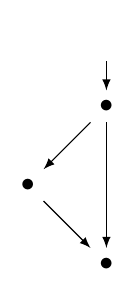
\begin{tikzpicture}
        \useasboundingbox (-1,-1) rectangle (0,2);
        \node at (0,1.7) (start) {};
        \node at (0,1)  (A) {$\bullet$};
        \node at (-1,0) (B) {$\bullet$};
        \node at (0,-1) (C) {$\bullet$};
        \draw[-latex] (start) -- (A);
        \draw[-latex] (A) -- (B);
        \draw[-latex] (A) -- (C);
        \draw[-latex] (B) -- (C);
      \end{tikzpicture}
    \end{center}
    \caption{\texttt{if} conditional}
    \label{if-figure}
  \end{subfigure}
  \begin{subfigure}{0.23\textwidth}
    \begin{center}
      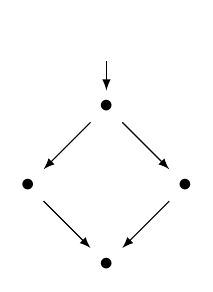
\begin{tikzpicture}
        \useasboundingbox (-1,-1) rectangle (1,2);
        \node at (0,1.7) (start) {};
        \node at (0,1)  (A) {$\bullet$};
        \node at (1,0)  (B) {$\bullet$};
        \node at (-1,0) (C) {$\bullet$};
        \node at (0,-1) (D) {$\bullet$};
        \draw[-latex] (start) -- (A);
        \draw[-latex] (A) -- (B);
        \draw[-latex] (A) -- (C);
        \draw[-latex] (B) -- (D);
        \draw[-latex] (C) -- (D);
      \end{tikzpicture}
    \end{center}
    \caption{\texttt{if}-\texttt{else} conditional}
    \label{if-else-figure}
  \end{subfigure}
  \begin{subfigure}{0.25\textwidth}
    \begin{center}
      \begin{tikzpicture}
        \useasboundingbox (-1,0) rectangle (1,3);
        \node at (0,1.7) (start) {};
        \node at (0,1)  (A) {$\bullet$};
        \node at (1,0)  (B) {$\bullet$};
        \node at (-1,0) (C) {$\bullet$};
        \draw[-latex] (start) -- (A);
        \draw[-latex] (A) -- (B);
        \draw[-latex] (A) -- (C);
      \end{tikzpicture}
    \end{center}
    \caption{divergent conditional}
    \label{divergent-figure}
  \end{subfigure} 
  \\
  \begin{subfigure}{0.32\textwidth}
    \begin{center}
      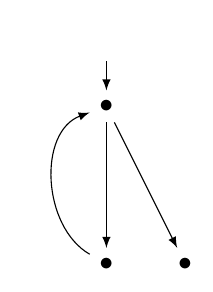
\begin{tikzpicture}
        \useasboundingbox (-1,-1) rectangle (1,2);
        \node at (0,1.7) (start) {};
        \node at (0,1) (A) {$\bullet$};
        \node at (0,-1) (B) {$\bullet$};
        \node at (1,-1) (C) {$\bullet$};
        \draw[-latex] (start) -- (A);
        \draw[-latex] (A) to (B);
        \draw[-latex] (A) to (C);
        \draw[-latex] (B) to[in=200,out=150] (A);
      \end{tikzpicture}
    \end{center}
    \caption{\texttt{while} loop}
    \label{while-figure}
  \end{subfigure}
  \begin{subfigure}{0.32\textwidth}
    \begin{center}
      \begin{tikzpicture}
        \useasboundingbox (-1,0) rectangle (1,3);
        \node at (0,1.7) (start) {};
        \node at (0,1)  (A) {$\bullet$};
        \node at (1,0)  (B) {$\bullet$};
        \draw[-latex] (start) -- (A);
        \draw[-latex] (A) to (B);
        \draw[-latex] (A) to[out=235,in=180,looseness=10] (A);
      \end{tikzpicture}
    \end{center}
    \caption{\texttt{do}-\texttt{while} loop}
    \label{do-while-figure}
  \end{subfigure}
  \begin{subfigure}{0.32\textwidth}
    \begin{center}
      \begin{tikzpicture}
        \useasboundingbox (-1,0) rectangle (1,3);
        \node at (0,1.7) (start) {};
        \node at (0,1)  (A) {$\bullet$};
        \draw[-latex] (start) -- (A);
        \draw[-latex] (A) to[out=270,in=180,looseness=10] (A);
      \end{tikzpicture}
    \end{center}
    \caption{infinite loop}
    \label{infinite-loop-figure}
  \end{subfigure}
  \caption{Control flow graphs of program structures}
  \label{structured-cfg-figures}
\end{figure}

Precisely, we require the control flow graph of each method in the
input program to have a structure based on Dijkstra's notion of
program structure found in~\cite{dijkstra1972}.
In our definition of a structured program, the control flow graph must
be composed of the structures shown in
Figure~\ref{structured-cfg-figures}. 
The first structure (Figure~\ref{sequence-figure}) is that of simple
sequential composition, with an edge going from the root node to a
single end node.
The next three structures
(Figure~\ref{if-figure}--\subref{divergent-figure}) are conditional
structures. 
Figure~\ref{if-figure} shows an \texttt{if} statement with no
\texttt{else} clause. 
Figure~\ref{if-else-figure} shows an \texttt{if} statement with an
\texttt{else} clause. 
Figure~\ref{divergent-figure} shows a conditional in which both
branches end with a (infinite) loop or a return so that there is
nothing following the conditional; we refer to such conditionals as
divergent conditionals since the branches do not come back together.
The remaining three structures
(Figure~\ref{while-figure}--\subref{infinite-loop-figure}) are all
loops.
Figure~\ref{while-figure} shows a loop in which the loop condition is
checked at the beginning (a \texttt{while} loop).
Figure~\ref{do-while-figure} shows a loop in which the loop condition
is checked at the end (a \texttt{do}-\texttt{while} loop).
Figure~\ref{infinite-loop-figure} shows an infinite loop.

We provide below a formal definition of what it means for a control
flow graph to be structured. 
This definition is based on that in~\cite{bento2017}, which provides
an algorithm for recognising structured graphs.
We first define a rooted directed graph below. 
The definition is standard, but we include it here to introduce the
terminology for the subsequent definition.
\begin{defn}[Rooted Directed Graph] A \emph{rooted directed graph},
$G$, is a triple $(V,E,r)$, where
  \begin{itemize}
  \item $V$ is a set of \emph{nodes},
  \item $E$ is a set of ordered pairs of nodes in $V$, called
\emph{edges}, and
  \item $r$ is a node in $V$, called the \emph{root} of the graph.
  \end{itemize}
  The first component of an edge is its \emph{source}
  and the second component is its \emph{target}. 
  We say that an edge goes from its source to its target. 
  For every node $n \in V$, the pair $(r,n)$ must be in the reflexive
  transitive closure of $E$, that is, there must be a path of edges
  from the root to any node in the graph.
  For a graph $G$, we refer to the set
  $T(G) = \{ n \in V | \forall m \in V.\; (n,m) \notin E\}$ of nodes
  with no edges coming from them as the set of \emph{end nodes} of the
  graph.
\end{defn}
In diagrams we represent the nodes as points or as the names of the
nodes, the edges as arrows, and the root node as a node with an arrow
pointing to it that does not come from another node.
Additionally, we refer to the source of an edge going to a given node
as a \emph{predecessor} of that node; similarly, the target of an edge
from a given node is a \emph{successor} of that node.

We now define what it means to replace a node in a graph by another
graph.
We use this concept to construct more complex structured graphs from
those shown in Figure~\ref{structured-cfg-figures}.
Node replacement may occur in four different ways, depending on which
node is being replaced in a graph.
We illustrate the different cases of node replacement using the
example graphs $G$ and $H$ shown in Figure~\ref{G-H-examples-figure}.
The $G$ graph has the form of a conditional with two branches, and the
$H$ graph has the form of a \texttt{while} loop.
We label the nodes of the graphs separately for ease of reference.

\begin{figure}
  \begin{center}
    \begin{tikzpicture}
      \useasboundingbox (-3,-2) rectangle (2,2);
      \node at (-1,2) {$G$};
      \node at (0,1.7) (start) {};
      \node at (0,1)  (A) {$1$};
      \node at (1,0)  (B) {$2$};
      \node at (-1,0) (C) {$3$};
      \node at (0,-1) (D) {$4$};
      \draw[-latex] (start) -- (A);
      \draw[-latex] (A) -- (B);
      \draw[-latex] (A) -- (C);
      \draw[-latex] (B) -- (D);
      \draw[-latex] (C) -- (D);
    \end{tikzpicture}
    \begin{tikzpicture}
      \useasboundingbox (-3,-2) rectangle (2,2);
      \node at (-1,2) {$H$};
      \node at (0,1.7) (start) {};
      \node at (0,1) (A) {$a$};
      \node at (0,-1) (B) {$b$};
      \node at (1,-1) (C) {$c$};
      \draw[-latex] (start) -- (A);
      \draw[-latex] (A) to (B);
      \draw[-latex] (A) to (C);
      \draw[-latex] (B) to[in=200,out=150] (A);
    \end{tikzpicture}
    \caption{Example control flow graphs to illustrate node
      replacement}
    \label{G-H-examples-figure}
  \end{center}
\end{figure}

The first case is that of placing a graph at the start of another
graph, i.e.\ replacing the root node of a graph that does not have a
loop to its root node.
An example of this can be seen in
Figure~\ref{root-replacement-figure}, where the root node (node $1$)
of graph $G$ is replaced with graph $H$.
The unique end node of graph $H$, node $c$, takes the place of node
$1$.
The other nodes of $H$ are connected to it by the same edges as in
$H$.

The second case is that of replacing one of the end nodes of a graph.
This is shown in Figure~\ref{end-replacement-figure}, where node $4$
of graph $G$ is replaced with graph $H$.
Node $a$, the root node of graph $H$, takes the place of node $4$.
As in the previous case, the remaining nodes of $H$ are included,
connected to $a$ by the same edges as in $H$.

The third case (Figure~\ref{internal-replacement-figure}) is that of
replacing an internal node of the graph.
In our example, node $2$ of graph $G$ is replaced with graph $H$.
There is an edge from the predecessor of node $2$, which is node $1$
in this case, to the root node of $H$ (node $a$).
There is another edge from the end node of $H$ (node $c$), which is
required to be unique, to the successor of node $3$, which is node $4$
in this case.

The final case, an example of which is shown in
Figure~\ref{branch-end-replacement-figure}, is where control flow
constructs occur at the end of one branch of a conditional.
In our example, node $2$ of graph $G$ is replaced with graph $H$, as
in the previous case, but the end node of $H$ (node $c$) is identified
with the successor of node $2$ (node $4$), and so it is not included
in the graph.
Thus, this represents the case in which no instructions occur inside
the conditional branch after the while loop.
Such instructions are represented by node $c$ in
Figure~\ref{internal-replacement-figure}, which is excluded in
Figure~\ref{branch-end-replacement-figure}.

\begin{figure}
  \begin{subfigure}{0.24\textwidth}
    \begin{center}
      \begin{tikzpicture}
        \useasboundingbox (-1.5,-2.5) rectangle (1.5,2);
        \node at (0,2) (start) {};
        \node at ( 0, 1)  (A) {$a$};
        \node at (-1, 0)  (B) {$b$};
        \node at ( 0,0)   (D) {$c$};
        \node at (-1,-1)  (E) {$2$};
        \node at ( 1,-1)  (F) {$3$};
        \node at ( 0,-2)  (G) {$4$};
        \draw[-latex] (start) -- (A);
        \draw[-latex] (A) to (B);
        \draw[-latex] (A) to (D);
        \draw[-latex] (B) to[in=180,out=90] (A);
        \draw[-latex] (D) -- (E);
        \draw[-latex] (D) -- (F);
        \draw[-latex] (E) -- (G);
        \draw[-latex] (F) -- (G);
      \end{tikzpicture}
    \caption{\centering root node\newline replacement}
    \label{root-replacement-figure}
  \end{center}
  \end{subfigure}
  \begin{subfigure}{0.24\textwidth}
    \begin{center}
      \begin{tikzpicture}
        \useasboundingbox (-1.5,-2.5) rectangle (1.5,2);
        \node at (0,2) (start) {};
        \node at ( 0, 1)  (A) {$1$};
        \node at (-1, 0)  (B) {$2$};
        \node at ( 1, 0)  (C) {$3$};
        \node at ( 0,-1)  (D) {$a$};
        \node at ( 0,-2)  (E) {$b$};
        \node at ( 1,-2)  (F) {$c$};
        \draw[-latex] (start) -- (A);
        \draw[-latex] (A) -- (B);
        \draw[-latex] (A) -- (C);
        \draw[-latex] (B) -- (D);
        \draw[-latex] (C) -- (D);
        \draw[-latex] (D) to (E);
        \draw[-latex] (D) to (F);
        \draw[-latex] (E) to[in=200,out=150] (D);
      \end{tikzpicture}
    \caption{\centering end node\newline replacement}
    \label{end-replacement-figure}
    \end{center}
  \end{subfigure}
  \begin{subfigure}{0.24\textwidth}
    \begin{center}
      \begin{tikzpicture}
        \useasboundingbox (-1.5,-2.5) rectangle (1.5,2);
        \node at (0,2) (start) {};
        \node at ( 0, 1)    (A) {$1$};
        \node at (-1, 0)    (B) {$a$};
        \node at ( 1,-0.5)  (C) {$3$};
        \node at (-2,-1)    (D) {$b$};
        \node at (-1,-1)    (F) {$c$};
        \node at ( 0,-2)    (G) {$4$};
        \draw[-latex] (start) -- (A);
        \draw[-latex] (A) -- (B);
        \draw[-latex] (A) -- (C);
        \draw[-latex] (B) to (D);
        \draw[-latex] (B) to (F);
        \draw[-latex] (D) to[in=180,out=90] (B);
        \draw[-latex] (F) -- (G);
        \draw[-latex] (C) -- (G);
      \end{tikzpicture}
      \caption{\centering internal node\newline replacement}
      \label{internal-replacement-figure}
    \end{center}
  \end{subfigure}
  \begin{subfigure}{0.24\textwidth}
    \begin{center}
      \begin{tikzpicture}
        \useasboundingbox (-1.5,-2.5) rectangle (1.5,2);
        \node at (0,2) (start) {};
        \node at ( 0, 1)    (A) {$1$};
        \node at (-1,-0.5)  (B) {$a$};
        \node at ( 1,-0.5)  (C) {$3$};
        \node at (-2,-1.5)  (D) {$b$};
        \node at ( 0,-2)    (G) {$4$};
        \draw[-latex] (start) -- (A);
        \draw[-latex] (A) -- (B);
        \draw[-latex] (A) -- (C);
        \draw[-latex] (B) to (D);
        \draw[-latex] (B) to (G);
        \draw[-latex] (D) to[in=180,out=90] (B);
        \draw[-latex] (C) -- (G);
      \end{tikzpicture}
    \caption{\centering branch end\newline replacement}
    \label{branch-end-replacement-figure}
  \end{center}
  \end{subfigure}
  \caption{Examples of the different cases of node replacement}
  \label{node-replacement-example-figures}
\end{figure}

In general, we define node replacement using the formal definition
below.
This covers each of the four cases shown above.
\begin{defn}[Node Replacement]
  Given two rooted directed graphs $G$ and $H$, we say $G'$ is the
  graph formed by \emph{replacing} a node $n$ of $G$ with $H$ if one
  of the following cases holds:
  \begin{itemize}
  \item $n$ has no predecessors in $G$, $H$ has only one end node, and
    \begin{itemize}
    \item $G'$ contains all the nodes of $H$ and $G$, except $n$,
    \item $G'$ contains the edges of $G$ except those going to or from
      $n$,
    \item $G'$ contains edges from the end node of $H$ to the
      successors of $n$ in $G$, and
    \item the root node of $G'$ is the root node of $H$;
    \end{itemize}
  \item $n$ has no successors in $G$, and
    \begin{itemize}
    \item $G'$ contains all the nodes of $H$ and $G$, except $n$,
    \item $G'$ contains the edges of $G$ except those going to or from
      $n$,
    \item $G'$ contains edges from the predecessors $n$ in $G$ to the
      root node of $H$, and
    \item the root node of $G'$ is the root node of $G$, or, if $n$ is
      the root node of $G$, the root node of $H$;
    \end{itemize}
  \item $H$ has a single end node and
    \begin{itemize}
    \item $G'$ contains all the nodes of $H$ and $G$, except $n$,
    \item $G'$ contains the edges of $G$ and the edges of $H$ except
      those going to or from $n$,
    \item $G'$ contains edges from the predecessors of $n$ in $G$ to
      the root node of $H$,
    \item $G'$ contains edges from the end node of $H$ to the
      successors of $n$ in $G$, and
    \item the root node of $G'$ is the root node of $G$, or, if $n$ is
      the root node of $G$, the root node of $H$;
    \end{itemize}
  \item $n$ has a single successor in $G$, $H$ has a single end
    node, and
    \begin{itemize}
    \item $G'$ contains all the nodes of $H$ and $G$, except $n$ and
      the end node of $H$,
    \item $G'$ contains the edges of $G$ except those going to or from
      $n$,
    \item $G'$ contains edges from the predecessors of the end node of
      $H$ to the successor of $n$ in $G$
    \item $G'$ contains edges from the predecessors of $n$ in $G$ to
      the root node of $H$, and
    \item the root node of $G'$ is the root node of $G$, or, if $n$ is
      the root node of $G$, the root node of $H$.
    \end{itemize}
  \end{itemize}
\end{defn}

With node replacement defined, we can now finally define what we mean
by a structure control flow graph in terms of node replacement and the
structured graphs shown in Figure~\ref{structured-cfg-figures}

\begin{defn}[Structured Control Flow Graph]
  If $G$ is a rooted directed graph, we say $G$ is a \emph{structured
    control flow graph} if $G$ is the trivial graph (the graph with a
  single node, which is also the root, and no edges) or if $G$ can be
  created by starting with the trivial graph and performing a finite
  number of node replacements to replace nodes with graphs of the
  forms shown in Figure~\ref{structured-cfg-figures}.
\end{defn}

Before applying the strategy, it must be ensured that the control flow
graph for each method is well-structured according to this definition.

We also require that integer operations are used only where integer
overflow cannot occur.
This is due to the fact that we follow icecap's approach and compile
addition in Java bytecode to addition in C, making the assumption that
the addition does not overflow, since overflow is undefined behaviour
in C.
The Java code should be written in a style consistent with MISRA-C,
where behaviours that are undefined in C must not be relied on.

We do not handle synchronisation of static methods, since icecap does
not apply synchronisation to static methods.
It is important that we follow the approach of a practical tool on
this, to ensure that our strategy can be implemented.
No expressive power is lost by forbidding static synchronized methods,
since a singleton instance of a class with synchronized methods can be
supplied, rather than relying on static methods to access data owned
by the instance.

Each method call must have at least one target (as
determined by the rules given in
Section~\ref{resolve-method-calls-subsection}), to allow method calls
to be resolved.
Each \texttt{invokestatic} and \texttt{invokespecial} instruction has
exactly one target, so this poperty is always fulfilled for such
method calls.
For \texttt{invokevirtual} instructions, a method call only has no
targets if the method in which the instruction occurs is unused or if
the method is invoked on a null pointer (which is erroneous).
Methods not used in the program should not be included in the
parameters passed to $CEE$, matching icecap's behaviour of excluding
such methods from the generated code.

Finally, we require that no method in the program recurses, either
directly or indirectly.
This is because recursion is not recommended in safety-critical
applications because of the potential for unpredictable failure due to
stack overflow, and it is not allowed in MISRA-C for that reason.
Imposing this requirement allows us to handle methods individually
when introducing their control flow, without considering circular
dependencies between them.

We now proceed to describe each of the stages of the strategy in
detail, beginning with the \emph{Elimination of Program Counter} stage
in the next section.

\section{Elimination of Program Counter}
\label{elimination-of-program-counter-section}

The first stage eliminates $pc$ from the state of each thread's
process, $Thr(bc,cs,instCS,t)$, introducing the control flow constructs of C
as a result. 
It is summarised by the following theorem.
%
\begin{thm}[Elimination of Program Counter]\label{epc-thm}
  \begin{circus}
    Thr(bc,cs,instCS,t) \circrefines ThrCF_{bc,cs}(cs,t)
  \end{circus}%
\end{thm}
%
We act mainly upon the $Running$ action of $Thr$; its loop is unrolled
to introduce the control flow that follows each bytecode instruction.
The aim is to get each method's bytecode instructions into a form in
which the control flow, but not the data operations, are described
using C constructs and, moreover, each path of execution (including
every branch of the conditionals) ends in a return instruction or a
loop.
We refer to a method in this form as a \emph{complete} method.

It is important to observe that it is possible to transform the
bytecode instructions of every method so that they become complete.
If we consider the control flow of a method beginning from that
method's entry point, each bytecode instruction reached must either be
a return instruction, or followed by another bytecode.
If another bytecode follows the bytecode's execution, then it must be
either a bytecode already considered, resulting in a loop, or one not
already considered.
Since there are finitely many bytecode instructions in a method, a
loop or return must eventually be reached.
Failure to do so would lead to an instruction beyond the end of the
method, which is forbidden by the structural restrictions on Java
bytecode that are checked during bytecode verification. 
% We assume bytecode input to our strategy will have undergone bytecode
% verification so this cannot happen.

When a method is complete, it can be defined by a separate \Circus{}
action.
When the code for all the methods has been separated out in this way,
the choice of bytecode instruction using the program counter value can
be removed and replaced with a choice over method identifiers.
Thus dependency on the program counter can be completely removed,
allowing it to be eliminated from the state of $Thr$.

The detailed description of the strategy for transforming $Thr$ in
this stage and achieving this elimination is provided by
Algorithm~\ref{epc-algorithm}.
It begins at line~\ref{algorithm-expand-bytecode} by expanding the
\Circus{} definitions of the bytecode instructions from the $bc$ map
into the $Running$ action, pulling out the program counter updates so
that they can be more easily manipulated.
In line~\ref{algorithm-introduce-forward-sequence}, simple sequential
compositions, that is, those that do not involve handling loops or
conditionals, are introduced.
% instructions that
% are followed by the execution of a bytecode instruction that is not
% part of the start or end of a conditional or loop are sequenced with
% the instructions following them.
After that, for each method, its loops and conditionals are introduced
in line~\ref{algorithm-introduce-loops-and-conditionals}. 
Afterwards, any complete methods are separated out, in
line~\ref{algorithm-separate-complete-methods}, and any method calls
involving completed methods are resolved by sequencing the method call
with the \Circus{} action representing the method, in
line~\ref{algorithm-resolve-method-calls}.

This is repeated until all methods have been separated out, as
indicated by the while loop in
line\added{s}~\ref{algorithm-method-loop}\added{
  to~\ref{algorithm-method-loop-end}}.
The $MainThread$ and $NotStarted$ actions are then refined in
line~\ref{algorithm-refine-main-actions} to provide a choice over
method identifiers, rather than $pc$ values, thus removing all uses of
$pc$ from the interpreter.
The $pc$ component is then removed from the state in
line~\ref{algorithm-remove-pc-from-state} of the algorithm.

\begin{algorithm}[tp!]
  \begin{algorithmic}[1]
    \State \Call{ExpandBytecode}{} \label{algorithm-expand-bytecode}
    \State \Call{IntroduceSequentialComposition}{} \label{algorithm-introduce-forward-sequence}
    \While{$\lnot$\Call{AllMethodsSeparated}{}} \label{algorithm-method-loop}
    \State \Call{IntroduceLoopsAndConditionals}{} \label{algorithm-introduce-loops-and-conditionals}
    \State \Call{SeparateCompleteMethods}{} \label{algorithm-separate-complete-methods}
    \State \Call{ResolveMethodCalls}{} \label{algorithm-resolve-method-calls}
    \EndWhile \label{algorithm-method-loop-end}
    \State \Call{RefineMainActions}{} \label{algorithm-refine-main-actions}
    \State \Call{RemovePCFromState}{} \label{algorithm-remove-pc-from-state}
  \end{algorithmic}
  \caption{Elimination of Program Counter}
  \label{epc-algorithm}
\end{algorithm}

Each of the procedures used in Algorithm~\ref{epc-algorithm} is
defined in a separate section in the sequel.
Beforehand, we give a more detailed overview of the strategy using an
example.

\subsection{Running Example}
\label{overview-subsection}

We explain the strategy in detail with an example, the Java code for
which is shown in Figure~\ref{example-code-figure}.
\begin{figure}[tp]
  \begin{center}
  \begin{minipage}{14cm}
  \begin{lstlisting}[basicstyle=\ttfamily\footnotesize,keywordstyle=\bf\footnotesize,language=Java,numbers=left,numberstyle=\tiny,stepnumber=1, numbersep=5pt,escapeinside={(*@}{@*)}]
public class TPK extends AperiodicEventHandler {

  public TPK(PriorityParameters priority,
             AperiodicParameters release,
             StorageParameters storage,
             ConfigurationParameters config) {
    super(priority, release, storage, config);
  }
      
  public void handleAsyncEvent() {
    ConsoleConnection console = new ConsoleConnection(null); (*@\label{example-ConsoleConnection-line}@*)
        
    InputStream input = console.openInputStream(); (*@\label{example-InputStream-line}@*)
    OutputStream output = console.openOutputStream(); (*@\label{example-OutputStream-line}@*)
        
    for(int i = 0; i <= 10; i = i + 1) { (*@\label{example-for-loop-line}@*)
      int y = f(input.read());
          
      if (y > 400) {
        output.write(0);
      } else {
        output.write(y);
      }
    }
  }
      
  public static int f(int x){
    return x + x + x + 5;
  }
      
}
\end{lstlisting}
\end{minipage}
\end{center}
  \caption{Our example program}
  \label{example-code-figure}
\end{figure}
Our example is based on the Trabb Pardo-Knuth
algorithm~\cite{knuth1980}, used for comparison of programming
languages, since it includes a variety of programming constructs that
provide a good test of the strategy.
We have simplified the algorithm by removing the reading into an
array, since our bytecode subset does not include array operations.
Adding arrays makes the example much longer, while not giving any
interesting insight into our compilation strategy.
As previously explained, extending the bytecode set considered to deal
with arrays is not difficult.

We have also written the example as an SCJ program, with the algorithm
as the body of an aperiodic event handler, \texttt{TPK}, one or more
instances of which can be registered as part of a mission and released
during mission execution.
As already mentioned, each release of the handler causes its
\texttt{handleAsyncEvent()} method to be executed.
This method creates an instance of a \texttt{ConsoleConnection}
(line~\ref{example-ConsoleConnection-line}), which is the only
standard input/output connection required by SCJ.
Instances of \texttt{InputStream} and \texttt{OutputStream} are then
obtained from the \texttt{ConsoleConnection}
(lines~\ref{example-InputStream-line}
and~\ref{example-OutputStream-line}).

After the input and output streams have been obtained, we enter a for
loop (line~\ref{example-for-loop-line}) in which an integer is read
from the \texttt{InputStream}, a static method \texttt{f()} is applied
to it, and the result is output if it is less than 400, otherwise, 0
is output.
The method \texttt{f()} takes an integer as input, multiplies it by 3
and adds 5 to it.

The \texttt{TPK} class is part of a larger program that includes other
classes, including a \texttt{Safelet}, a \texttt{MissionSequencer}, a
\texttt{Mission}, and the classes that make up the SCJ API.
% Considering these classes in our example would make the example much
% larger and more complex, while not introducing any more interesting
% aspects for the strategy to consider.
We omit a presentation of these classes, though it should be noted
that they are part of the complete example.
For compilation, they need to go through a similar refinement to that
we illustrate for the $TPK$ class.
This adds little complexity to the strategy since the bytecode array
is acted upon consistently for all classes, and the current class of a
given bytecode instruction can always be determined from its address
in the array.

The Java code must be run through a Java compiler to generate the
corresponding bytecode, which then defines the $bc$ and $cs$ constants
of our model.
Their values for our example are shown in
Figure~\ref{example-model-figure}, along with $TPK$ class information.
While most of the compilation of the methods of \texttt{TPK} depends
only on the data in the $TPK$ class information, the object data for
instances of \texttt{TPK} includes fields from its superclasses.
In particular, the fields for \texttt{TPK} are contributed by the
\texttt{AperiodicEventHandler} and \texttt{ManagedEventHandler}
classes (the superclasses of \texttt{ManagedEventHandler} do not
contribute any fields), whose $Class$ data structures are presented in
Figure~\ref{example-superclasses-model-figure}.
The generation of object structures from this field information is
discussed in more detail in
Section~\ref{data-refinement-of-objects-section}.

\begin{figure}[p]
  \begin{center}
  \setlength{\linewidth}{12cm}
  \begin{tabular}{p{9.5cm}p{4.5cm}}
    \scriptsize
    \setlength{\zedindent}{0cm}
    \setlength{\zedtab}{0.3cm}
    \setlength{\zedleftsep}{0cm}
    \begin{axdef}
      TPK : Class
    \where
      TPK = \lblot \\
      \t1 constantPool == \{ \\
      \t2 1 \mapsto ClassRef~TPKClassID, \\
      \t2 3 \mapsto ClassRef~AperiodicEventHandlerClassID, \\
      \t2 8 \mapsto MethodRef~AperiodicEventHandlerClassID~APEHinit, \\
      \t2 27 \mapsto ClassRef~ConsoleConnectionClassID, \\
      \t2 29 \mapsto  MethodRef~ConsoleConnectionClassID~CCinit, \\
      \t2 32 \mapsto MethodRef~ConsoleConnectionClassID~openInputStream, \\
      \t2 36 \mapsto MethodRef~ConsoleConnectionClassID~openOutputStream, \\
      \t2 40 \mapsto MethodRef~InputStreamClassID~read, \\
      \t2 41 \mapsto ClassRef~InputStreamClassID, \\
      \t2 46 \mapsto MethodRef~TPKClassID~f, \\
      \t2 50 \mapsto MethodRef~OutputStreamClassID~write, \\
      \t2 51 \mapsto ClassRef~OutputStreamClassID \\
      \t1 \}, \\
      \t1 this == 1, \\
      \t1 super == 3, \\
      \t1 interfaces == \{\}, \\
      \t1 methodEntry == \{ \\
      \t2 f \mapsto 43, \\
      \t2 handleAsyncEvent \mapsto 7, \\
      \t2 APEHinit \mapsto 0, \\
      \t1 \}, \\
      \t1 methodEnd == \{ \\
      \t2 f \mapsto 50, \\
      \t2 handleAsyncEvent \mapsto 42, \\
      \t2 APEHinit \mapsto 6 \\
      \t1 \}, \\
      \t1 methodLocals == \{ \\
      \t2 f \mapsto 1, \\
      \t2 handleAsyncEvent \mapsto 6, \\
      \t2 APEHinit \mapsto 5, \\
      \t1 \}, \\
      \t1 methodStackSize == \{ \\
      \t2 f \mapsto 2, \\
      \t2 handleAsyncEvent \mapsto 3, \\
      \t2 APEHinit \mapsto 5, \\
      \t1 \}, \\
      \t1 staticMethods == \{ f \} \\
      \t1 fields == \{\}, \\
      \t1 staticFields == \{\} \\
      \rblot
    \end{axdef}
    \begin{axdef}
      cs : ClassID \pfun Class
      \where
      cs = \{ \\
      \t1 TPKClassID \mapsto TPK, \\
      \t1 AperiodicEventHandlerClassID \mapsto AperiodicEventHandler, \\
      \t1 ManagedEventHandlerClassID \mapsto ManagedEventHandler, \\
      \t1 \cdots \\
      \}
    \end{axdef}
    &
    \scriptsize
    \setlength{\zedindent}{0cm}
    \setlength{\zedtab}{0.3cm}
    \setlength{\zedleftsep}{0cm}
    \begin{axdef}
      bc : ProgramAddress \pfun Bytecode
      \where
      bc = \{ \\
      	\t1 0 \mapsto aload~0, \\
        \t1 1 \mapsto aload~1, \\
        \t1 2 \mapsto aload~2, \\
        \t1 3 \mapsto aload~3, \\
        \t1 4 \mapsto aload~4, \\
        \t1 5 \mapsto invokespecial~8, \\
        \t1 6 \mapsto return, \\
        \t1 7 \mapsto new~27, \\
        \t1 8 \mapsto dup, \\
        \t1 9 \mapsto aconst\_null, \\
        \t1 10 \mapsto invokespecial~29, \\
        \t1 11 \mapsto astore~1, \\
        \t1 12 \mapsto aload~1, \\
        \t1 13 \mapsto invokevirtual~32, \\
        \t1 14 \mapsto astore~2, \\
        \t1 15 \mapsto aload~1, \\
        \t1 16 \mapsto invokevirtual~36, \\
        \t1 17 \mapsto astore~3, \\
        \t1 18 \mapsto iconst~0, \\
        \t1 19 \mapsto astore~4, \\
        \t1 20 \mapsto goto~19, \\
        \t1 21 \mapsto aload~2, \\
        \t1 22 \mapsto invokevirtual~40, \\
        \t1 23 \mapsto invokestatic~46, \\
        \t1 24 \mapsto astore~5, \\
        \t1 25 \mapsto aload~5, \\
        \t1 26 \mapsto iconst~400, \\
        \t1 27 \mapsto if\_icmple~5, \\
        \t1 28 \mapsto aload~3, \\
        \t1 29 \mapsto iconst~0, \\
        \t1 30 \mapsto invokevirtual~50, \\
        \t1 31 \mapsto goto~4, \\
        \t1 32 \mapsto aload~3, \\
        \t1 33 \mapsto aload~5, \\
        \t1 34 \mapsto invokevirtual~50, \\
        \t1 35 \mapsto aload~4, \\
        \t1 36 \mapsto iconst~1, \\
        \t1 37 \mapsto iadd, \\
        \t1 38 \mapsto astore~4, \\
        \t1 39 \mapsto aload~4, \\
        \t1 40 \mapsto iconst~10, \\
        \t1 41 \mapsto if\_icmple~(\negate 20), \\
        \t1 42 \mapsto return, \\
        \t1 43 \mapsto aload~0, \\
        \t1 44 \mapsto aload~0, \\
        \t1 45 \mapsto iadd, \\
        \t1 46 \mapsto aload~0, \\
        \t1 47 \mapsto iadd, \\
        \t1 48 \mapsto iconst~5, \\
        \t1 49 \mapsto iadd, \\
        \t1 50 \mapsto areturn, \\
        \t1 {} \cdots {} \\
        \}
      \end{axdef}
  \end{tabular}
  \end{center}
  \caption{The \Circus{} code corresponding to our example program}
  \label{example-model-figure}
\end{figure}%

\begin{figure}[tp!]
  \begin{center}
    % \setlength{\linewidth}{12cm}
    \begin{minipage}{7.5cm}
      \scriptsize
      \setlength{\abovedisplayskip}{0cm}
      \setlength{\belowdisplayskip}{0cm}
      \setlength{\zedindent}{0cm}
      \setlength{\zedtab}{0.3cm}
      \setlength{\zedleftsep}{0cm}
    \begin{axdef}
      AperiodicEventHandler : Class
    \where
      AperiodicEventHandler = \lblot \\
      \t1 constantPool == \{ \\
      \t2 1 \mapsto ClassRef~AperiodicEventHandlerClassID, \\
      \t2 3 \mapsto ClassRef~ManagedEventHandlerClassID, \\
      % \t2 8 \mapsto MethodRef~ManagedEventHandlerClassID~MEHinit, \\
      \t2 {} \cdots {} \\
      % \t2 11 \mapsto FieldRef~AperiodicEventHandler~priority, \\
      % \t2 15 \mapsto FieldRef~AperiodicEventHandler~backingStoreSpace, \\
      % \t2 18 \mapsto FieldRef~AperiodicEventHandler~allocAreaSpace, \\
      % \t2 21 \mapsto FieldRef~AperiodicEventHandler~stackSize, \\
      % \t2 24 \mapsto MethodRef~AperiodicEventHandler~initAPEH, \\
      % \t2 40 \mapsto MethodRef~AperiodicEventHandler~releaseAperiodic \\
      \t1 \}, \\
      \t1 this == 1, \\
      \t1 super == 3, \\
      \t1 interfaces == \{\}, \\
      \t1 methodEntry == \{ {} \cdots {}
      % \t2 MEHinit \mapsto 0, \\
      % \t2 release \mapsto 16 \\
      \}, \\
      \t1 methodEnd == \{ {} \cdots {}
      % \t2 MEHinit \mapsto 15, \\
      % \t2 release \mapsto 18 \\
      \}, \\
      \t1 methodLocals == \{ {} \cdots {}
      % \t2 MEHinit \mapsto 5, \\
      % \t2 release \mapsto 1 \\
      \}, \\
      \t1 methodStackSize == \{ {} \cdots {} 
      % \t2 MEHinit \mapsto 5, \\
      % \t2 release \mapsto 1 \\
      \}, \\
      \t1 fields == \{\}, \\
      \t1 staticFields == \{\} \\
      \rblot
    \end{axdef}%
  \end{minipage}
  \hfill
  \begin{minipage}{8cm}
    \scriptsize
    \setlength{\zedindent}{0cm}
    \setlength{\zedtab}{0.3cm}
    \setlength{\zedleftsep}{0cm}
    \begin{axdef}
      ManagedEventHandler : Class
    \where
      ManagedEventHandler = \lblot \\
      \t1 constantPool == \{ \\
      \t2 1 \mapsto ClassRef~ManagedEventHandlerClassID, \\
      \t2 3 \mapsto ClassRef~BoundAsyncEventHandlerClassID, \\
      \t2 5 \mapsto ClassRef~ManagedSchedulableClassID, \\
      % \t2 15 \mapsto MethodRef~BoundAsyncEventHandlerClassID~BAEHinit, \\
      \t2 {} \cdots {} \\
      % \t2 18 \mapsto MethodRef~PriorityParameters~getPriority, \\
      % \t2 19 \mapsto ClassRef~PriorityParameters, \\
      % \t2 24 \mapsto FieldRef~ManagedEventHandler~priority, \\
      % \t2 26 \mapsto MethodRef~ScopeParameters~getMaxInitialBackingStore, \\
      % \t2 27 \mapsto ClassRef~ScopeParameters, \\
      % \t2 32 \mapsto FieldRef~ManagedEventHandler~backingStoreSpace, \\
      % \t2 34 \mapsto MethodRef~ScopeParameters~getMaxInitialArea, \\
      % \t2 37 \mapsto FieldRef~ManagedEventHandler~allocAreaSpace, \\
      % \t2 39 \mapsto MethodRef~ConfigurationParameters~getSizes, \\
      % \t2 40 \mapsto ClassRef~ConfigurationParameters, \\
      % \t2 45 \mapsto MethodRef~LongArray~load, \\
      % \t2 46 \mapsto ClassRef~LongArray, \\
      % \t2 51 \mapsto FieldRef~ManagedEventHandler~stackSize, \\
      % \t2 66 \mapsto MethodRef~ManagedEventHandler~register \\
      \t1 \}, \\
      \t1 this == 1, \\
      \t1 super == 3, \\
      \t1 interfaces == \{5\}, \\
      \t1 methodEntry == \{ {} \cdots {}
      % \t2 MEHinit \mapsto 19, \\
      % \t2 getName \mapsto 41, \\
      % \t2 signalTermination \mapsto 46, \\
      % \t2 cleanUp \mapsto 40, \\
      % \t2 register \mapsto 43 \\
      \}, \\
      \t1 methodEnd == \{ {} \cdots {}
      % \t2 MEHinit \mapsto 39, \\
      % \t2 getName \mapsto 42, \\
      % \t2 signalTermination \mapsto 46, \\
      % \t2 cleanUp \mapsto 40, \\
      % \t2 register \mapsto 45 \\
      \}, \\
      \t1 methodLocals == \{ {} \cdots {}
      % \t2 MEHinit \mapsto 4, \\
      % \t2 getName \mapsto 1, \\
      % \t2 signalTermination \mapsto 1, \\
      % \t2 cleanUp \mapsto 1, \\
      % \t2 register \mapsto 1 \\
      \}, \\
      \t1 methodStackSize == \{ {} \cdots {}
      % \t2 MEHinit \mapsto 3, \\
      % \t2 getName \mapsto 1, \\
      % \t2 signalTermination \mapsto 0, \\
      % \t2 cleanUp \mapsto 0, \\
      % \t2 register \mapsto 1 \\
      \}, \\
      \t1 fields == \{ \\
      \t2 threadID, \\
      \t2 backingStoreSpace, \\
      \t2 allocAreaSpace, \\
      \t2 stackSize \\
      \t1 \}, \\
      \t1 staticFields == \{\} \\
      \rblot
    \end{axdef}
  \end{minipage}
  \end{center}
  \caption{The $Class$ structures for \texttt{AperiodicEventHandler}
    and \texttt{ManagedEventHandler}}
  \label{example-superclasses-model-figure}
\end{figure}%

Applying the bytecode expansion on
line~\ref{algorithm-expand-bytecode} of Algorithm~\ref{epc-algorithm}
yields the $Running$ action shown in
Figure~\ref{bytecode-expansion-example-figure}.
\begin{figure}[tp]
  \setlength{\zedindent}{0cm}
  \setlength{\zedtab}{0.3cm}
  \setlength{\zedleftsep}{0.1cm}
  \begin{circus}
    Running \circdef \\
    \t1 \circif frameStack = \emptyset \circthen \Skip \\
    \t1 {} \circelse frameStack \neq \emptyset \circthen {} \\
    \t2 \circif pc = 0 \circthen HandleAloadEPC(0) \circseq pc := 1 \\
    \t2 {} \circelse pc = 1 \circthen HandleAloadEPC(1) \circseq pc := 2 \\
    \t2 {} \circelse pc = 2 \circthen HandleAloadEPC(2) \circseq pc := 3 \\
    \t2 {} \circelse pc = 3 \circthen HandleAloadEPC(3) \circseq pc := 4 \\
    \t2 {} \circelse pc = 4 \circthen HandleAloadEPC(4) \circseq pc := 5 \\
    \t2 {} \circelse pc = 5 \circthen \{ pc = 5 \} \circseq HandleInvokespecialEPC(8) \\
    \t2 {} \circelse pc = 6 \circthen HandleReturnEPC \\
    \t2 {} \circelse pc = 7 \circthen HandleNewEPC(27) \circseq pc := 8 \\
    \t2 {} \circelse pc = 8 \circthen HandleDupEPC \circseq pc := 9 \\
    \t2 {} \circelse pc = 9 \circthen HandleAconst\_nullEPC \circseq pc := 10 \\
    \t2 {} \circelse pc = 10 \circthen \{ pc = 10 \} \circseq HandleInvokespecialEPC(29) \\
    \t2 {} \circelse pc = 11 \circthen HandleAstoreEPC(1) \circseq pc := 12 \\
    % \t2 {} \circelse pc = 12 \circthen HandleAloadEPC(1) \circseq pc := 13 \\
    % \t2 {} \circelse pc = 13 \circthen HandleInvokevirtualEPC(32) \\
    % \t2 {} \circelse pc = 14 \circthen HandleAstoreEPC(2) \circseq pc := 15 \\
    % \t2 {} \circelse pc = 15 \circthen HandleAloadEPC(1) \circseq pc := 16 \\
    % \t2 {} \circelse pc = 16 \circthen HandleInvokevirtualEPC(36) \\
    % \t2 {} \circelse pc = 17 \circthen HandleAstoreEPC(3) \circseq pc := 18 \\
    % \t2 {} \circelse pc = 18 \circthen HandleIconstEPC(0) \circseq pc := 19 \\
    % \t2 {} \circelse pc = 19 \circthen HandleAstoreEPC(4) \circseq pc := 20 \\
    % \t2 {} \circelse pc = 20 \circthen pc := 39 \\
    \t2 {} \cdots {} \\
    % \t2 {} \circelse pc = 21 \circthen HandleAloadEPC(2) \circseq pc := 22 \\
    % \t2 {} \circelse pc = 22 \circthen HandleInvokevirtualEPC(40) \\
    % \t2 {} \circelse pc = 23 \circthen HandleInvokestaticEPC(46) \\
    % \t2 {} \circelse pc = 24 \circthen HandleAstoreEPC(5) \circseq pc := 25 \\
    % \t2 {} \circelse pc = 25 \circthen HandleAloadEPC(5) \circseq pc := 26 \\
    % \t2 {} \circelse pc = 26 \circthen HandleIconstEPC(400) \circseq pc := 27 \\
    % \t2 {} \circelse pc = 27 \circthen \circvar value1, value2 : Word \circspot InterpreterPop2 \circseq \\
    % \t3 pc := \IF value1 \leq value2 \THEN 32 \ELSE 28 \\
    % \t2 {} \circelse pc = 28 \circthen HandleAloadEPC(3) \circseq pc := 29 \\
    % \t2 {} \circelse pc = 29 \circthen HandleIconstEPC(0) \circseq pc := 30 \\
    % \t2 {} \circelse pc = 30 \circthen HandleInvokevirtualEPC(50) \\
    % \t2 {} \circelse pc = 31 \circthen pc := 35 \\
    % \t2 {} \circelse pc = 32 \circthen HandleAloadEPC(3) \circseq pc := 33 \\
    % \t2 {} \circelse pc = 33 \circthen HandleAloadEPC(5) \circseq pc := 34 \\
    % \t2 {} \circelse pc = 34 \circthen HandleInvokevirtualEPC(50) \\
    % \t2 {} \circelse pc = 35 \circthen HandleAloadEPC(4) \circseq pc := 36 \\
    % \t2 {} \circelse pc = 36 \circthen HandleIconstEPC(1) \circseq pc := 37 \\
    % \t2 {} \circelse pc = 37 \circthen HandleIaddEPC \circseq pc := 38 \\
    % \t2 {} \circelse pc = 38 \circthen HandleAstoreEPC(4) \circseq pc := 39 \\
    % \t2 {} \circelse pc = 39 \circthen HandleAloadEPC(4) \circseq pc := 40 \\
    % \t2 {} \circelse pc = 40 \circthen HandleIconstEPC(10) \circseq pc := 41 \\
    % \t2 {} \circelse pc = 41 \circthen \circvar value1, value2 : Word \circspot InterpreterPop2 \circseq \\
    % \t3 pc := \IF value1 \leq value2 \THEN 21 \ELSE 42 \\
    % \t2 {} \circelse pc = 42 \circthen HandleReturnEPC \\
    % \t2 {} \circelse pc = 43 \circthen HandleAloadEPC(0) \circseq pc := 44 \\
    % \t2 {} \circelse pc = 44 \circthen HandleAloadEPC(0) \circseq pc := 45 \\
    % \t2 {} \circelse pc = 45 \circthen HandleIaddEPC \circseq pc := 46 \\
    % \t2 {} \circelse pc = 46 \circthen HandleAloadEPC(0) \circseq pc := 47 \\
    % \t2 {} \circelse pc = 47 \circthen HandleIaddEPC \circseq pc := 48 \\
    % \t2 {} \circelse pc = 48 \circthen HandleIconstEPC(5) \circseq pc := 49 \\
    % \t2 {} \circelse pc = 49 \circthen HandleIaddEPC \circseq pc := 50 \\
    % \t2 {} \circelse pc = 50 \circthen HandleAreturnEPC \\
    \t2 \circfi \circseq Poll \circseq Running \\
    \t1 \circfi
  \end{circus}
  \caption{The $Running$ action after bytecode expansion}
  \label{bytecode-expansion-example-figure}
\end{figure}
This step copies $HandleInstruction$ into $Running$, and converts it
to a choice of actions based on the value of the program counter,
$pc$, mirroring the contents of the $bc$ map for each value.

The actions that make up $HandleInstruction$ are also replaced with
actions that incorporate instruction parameters from the $bc$ map, and
have $pc$ updates separated from stack updates.
This can be seen in Figure~\ref{bytecode-expansion-example-figure},
where, for instance, in the $pc = 0$ case, $aload~0$ has been
converted to $HandleAloadEPC(0) \circseq pc := 1$, with the parameter,
$0$, to the bytecode instruction becoming a parameter of the new
instruction handling action $HandleAloadEPC$, and the update to $pc$
placed after the data operation.

The reason for making parameters of the bytecode instructions into
parameters of the handling actions is to remove the need to reference
the bytecode instructions in the $bc$ map, as that involves use of the
$pc$ value, which we seek to remove in this stage.
This also has the benefit of fully incorporating $bc$ into the $Thr$
process, ensuring all the information required to introduce C code
constructs is available directly in \Circus{}.
This makes stating compilation laws simpler, and is described in more
detail in Section~\ref{expand-bytecode-subsection}, where we define
the \Call{ExpandBytecode}{} procedure.

\begin{figure}[t!]
  \setlength{\zedindent}{0cm}
  \setlength{\zedtab}{0.3cm}
  \setlength{\zedleftsep}{0.1cm}
  \begin{circus}
    Running \circdef \\
    \t1 \circif frameStack = \emptyset \circthen \Skip \\
    \t1 {} \circelse frameStack \neq \emptyset \circthen {} \\
    \t2 \circif pc = 0 \circthen HandleAloadEPC(0) \circseq pc := 1 \circseq Poll \circseq HandleAloadEPC(1) \circseq \\
    \t3 pc := 2 \circseq Poll \circseq HandleAloadEPC(2) \circseq pc := 3 \circseq Poll \circseq HandleAloadEPC(4) \circseq \\
    \t3 pc := 5 \circseq Poll \circseq \{ pc = 5 \} \circseq HandleInvokespecialEPC(8) \\
    \t2 {} \cdots {} \\
    % \t2 {} \circelse pc = 1 \circthen HandleAloadEPC(1) \circseq pc := 2 \\
    % \t2 {} \circelse pc = 2 \circthen HandleAloadEPC(2) \circseq pc := 3 \\
    % \t2 {} \circelse pc = 3 \circthen HandleAloadEPC(3) \circseq pc := 4 \\
    % \t2 {} \circelse pc = 4 \circthen HandleAloadEPC(4) \circseq pc := 5 \\
    % \t2 {} \circelse pc = 5 \circthen HandleInvokespecialEPC(8) \\
    \t2 {} \circelse pc = 6 \circthen HandleReturnEPC \\
    \t2 {} \circelse pc = 7 \circthen HandleNewEPC(27) \circseq pc := 8 \circseq Poll \circseq HandleDupEPC \circseq pc := 9 \circseq Poll \circseq \\
    \t3 HandleAconst\_nullEPC \circseq pc := 10 \circseq Poll \circseq \{ pc = 10 \} \circseq HandleInvokespecialEPC(29) \\
    \t2 {} \cdots {} \\
    % \t2 {} \circelse pc = 8 \circthen HandleDupEPC \circseq pc := 9 \\
    % \t2 {} \circelse pc = 9 \circthen HandleAconst\_nullEPC \circseq pc := 10 \\
    % \t2 {} \circelse pc = 10 \circthen HandleInvokespecialEPC(29) \\
    % \t2 {} \circelse pc = 11 \circthen HandleAstoreEPC(1) \circseq pc := 12 \circseq Poll \circseq HandleAloadEPC(1) \circseq \\
    % \t3 pc := 13 \circseq Poll \circseq HandleInvokevirtualEPC(32) \\
    % \t2 {} \cdots {} \\
    % \t2 {} \circelse pc = 12 \circthen HandleAloadEPC(1) \circseq pc := 13 \\
    % \t2 {} \circelse pc = 13 \circthen HandleInvokevirtualEPC(32) \\
    \t2 {} \circelse pc = 14 \circthen HandleAstoreEPC(2) \circseq pc := 15 \circseq Poll \circseq HandleAloadEPC(1) \circseq \\
    \t3 pc := 16 \circseq Poll \circseq \{ pc = 16 \} \circseq HandleInvokevirtualEPC(36) \\
    \t2 {} \cdots {} \\
    % \t2 {} \circelse pc = 15 \circthen HandleAloadEPC(1) \circseq pc := 16 \\
    % \t2 {} \circelse pc = 16 \circthen HandleInvokevirtualEPC(36) \\
    \t2 {} \circelse pc = 17 \circthen HandleAstoreEPC(3) \circseq pc := 18 \circseq Poll \circseq HandleIconstEPC(0) \circseq \\
    \t3 pc := 19 \circseq Poll \circseq HandleAstoreEPC(4) \circseq pc := 20 \circseq Poll \circseq pc := 39 \\
    \t2 {} \cdots {} \\
    % \t2 {} \circelse pc = 18 \circthen HandleIconstEPC(0) \circseq pc := 19 \\
    % \t2 {} \circelse pc = 19 \circthen HandleAstoreEPC(4) \circseq pc := 20 \\
    % \t2 {} \circelse pc = 20 \circthen pc := 39 \\
    % \t2 {} \circelse pc = 21 \circthen HandleAloadEPC(2) \circseq pc := 22 \circseq Poll \circseq HandleInvokevirtualEPC(40) \\
    % \t2 {} \circelse pc = 22 \circthen HandleInvokevirtualEPC(40) \\
    % \t2 {} \circelse pc = 23 \circthen HandleInvokestaticEPC(46) \\
    % \t2 {} \circelse pc = 24 \circthen HandleAstoreEPC(5) \circseq pc := 25 \circseq Poll \circseq HandleAloadEPC(5) \circseq \\
    % \t3 pc := 26 \circseq Poll \circseq HandleIconstEPC(400) \circseq pc := 27 \circseq Poll \circseq \\
    % \t3 \circvar value1, value2 : Word \circspot InterpreterPop2 \circseq \\
    % \t3 pc := \IF value1 \leq value2 \THEN 32 \ELSE 28 \\
    % \t2 {} \circelse pc = 25 \circthen HandleAloadEPC(5) \circseq pc := 26 \\
    % \t2 {} \circelse pc = 26 \circthen HandleIconstEPC(400) \circseq pc := 27 \\
    % \t2 {} \circelse pc = 27 \circthen \circvar value1, value2 : Word \circspot InterpreterPop2 \circseq \\
    % \t3 pc := \IF value1 \leq value2 \THEN 32 \ELSE 28 \\
    % \t2 {} \circelse pc = 28 \circthen HandleAloadEPC(3) \circseq pc := 29 \circseq Poll \circseq HandleIconstEPC(0) \circseq \\
    % \t3 pc := 30 \circseq Poll \circseq HandleInvokevirtualEPC(50) \\
    % \t2 {} \circelse pc = 29 \circthen HandleIconstEPC(0) \circseq pc := 30 \\
    % \t2 {} \circelse pc = 30 \circthen HandleInvokevirtualEPC(50) \\
    % \t2 {} \circelse pc = 31 \circthen pc := 35 \\
    % \t2 {} \circelse pc = 32 \circthen HandleAloadEPC(3) \circseq pc := 33 \circseq Poll \circseq HandleAloadEPC(5) \circseq \\
    % \t3 pc := 34 \circseq Poll \circseq HandleInvokevirtualEPC(50) \\
    % \t2 {} \circelse pc = 33 \circthen HandleAloadEPC(5) \circseq pc := 34 \\
    % \t2 {} \circelse pc = 34 \circthen HandleInvokevirtualEPC(50) \\
    % \t2 {} \circelse pc = 35 \circthen HandleAloadEPC(4) \circseq pc := 36 \circseq Poll \circseq HandleIconstEPC(1) \circseq \\
    % \t3 pc := 37 \circseq Poll \circseq HandleIaddEPC \circseq pc := 38 \circseq Poll \circseq HandleAstoreEPC(4) \circseq \\
    % \t3 pc := 39 \\
    % \t2 {} \circelse pc = 36 \circthen HandleIconstEPC(1) \circseq pc := 37 \\
    % \t2 {} \circelse pc = 37 \circthen HandleIaddEPC \circseq pc := 38 \\
    % \t2 {} \circelse pc = 38 \circthen HandleAstoreEPC(4) \circseq pc := 39 \\
    \t2 {} \circelse pc = 39 \circthen HandleAloadEPC(4) \circseq pc := 40 \circseq Poll \circseq HandleIconstEPC(10) \circseq \\
    \t3 pc := 41 \circseq Poll \circseq \circvar value1, value2 : Word \circspot InterpreterPop2 \circseq \\
    \t3 pc := \IF value1 \leq value2 \THEN 21 \ELSE 42 \\
    \t2 {} \cdots {} \\
    % \t2 {} \circelse pc = 40 \circthen HandleIconstEPC(10) \circseq pc := 41 \\
    % \t2 {} \circelse pc = 41 \circthen \circvar value1, value2 : Word \circspot InterpreterPop2 \circseq \\
    % \t3 pc := \IF value1 \leq value2 \THEN 21 \ELSE 42 \\
    \t2 {} \circelse pc = 42 \circthen HandleReturnEPC \\
    \t2 {} \circelse pc = 43 \circthen HandleAloadEPC(0) \circseq pc := 44 \circseq Poll \circseq HandleAloadEPC(0) \circseq \\
    \t3 pc := 45 \circseq Poll \circseq HandleIaddEPC \circseq pc := 46 \circseq Poll \circseq HandleAloadEPC(0) \circseq \\
    \t3 pc := 47 \circseq Poll \circseq HandleIaddEPC \circseq pc := 48 \circseq Poll \circseq HandleIaddEPC \circseq \\
    \t3 pc := 50 \circseq Poll \circseq HandleAreturnEPC \\
    \t2 {} \cdots {} \\
    % \t2 {} \circelse pc = 44 \circthen HandleAloadEPC(0) \circseq pc := 45 \\
    % \t2 {} \circelse pc = 45 \circthen HandleIaddEPC \circseq pc := 46 \\
    % \t2 {} \circelse pc = 46 \circthen HandleAloadEPC(0) \circseq pc := 47 \\
    % \t2 {} \circelse pc = 47 \circthen HandleIaddEPC \circseq pc := 48 \\
    % \t2 {} \circelse pc = 48 \circthen HandleIconstEPC(5) \circseq pc := 49 \\
    % \t2 {} \circelse pc = 49 \circthen HandleIaddEPC \circseq pc := 50 \\
    % \t2 {} \circelse pc = 50 \circthen HandleAreturnEPC \\
    \t2 \circfi \circseq Poll \circseq Running \\
    \t1 \circfi
  \end{circus}
  \caption{The $Running$ action after forward sequence introduction}
  \label{forward-sequence-introduction-example-figure}
\end{figure}

On line~\ref{algorithm-introduce-forward-sequence} of the
Algorithm~\ref{epc-algorithm}, sequential composition is introduced
for instructions that do not affect the sequential flow of the
program.
Such instructions are identified by considering the control flow graph
of the program and locating nodes with a single outgoing edge going to
a target node with exactly one incoming edge.
The introduction of sequential composition is performed by unrolling
the loop in $Running$ to introduce the control flow following each of
these instructions.
This causes the instruction to be sequentially composed with the next
instruction, with $Poll$ inbetween to allow for thread switches
between instructions.
This is performed exhaustively to get the code in the form shown in
Figure~\ref{forward-sequence-introduction-example-figure}, where the
choice over $pc$ has sequences of instructions collected together at
the point where they start, up to the point at which a more complex
control flow (such as a method call, conditional or a loop) occurs.
The introduction of sequential composition is described in more detail
in Section~\ref{introduce-forward-sequence-subsection}, where we
define the \Call{IntroduceSequentialComposition}{} procedure.

Handling the remaining constructs requires consideration of
dependencies between methods to ensure method calls can be resolved
correctly.
We say a method call is \emph{resolved} when the method invocation
bytecode has been placed in sequential composition with a call to a
\Circus{} action containing the body of the method being invoked,
which is then followed by the sequence of instructions that occurs
after the invocation bytecode in the calling method.
After a method call has been resolved, it no longer breaks up the
sequence of instructions it occurs in.
%TODO: clarify this

Since we have the bytecode instructions of all the methods needed, we
can always resolve the call of a complete method, provided that method
has already been split into its own \Circus{} action.
To obtain a complete method, we first perform loop and conditional
introduction upon the method.
Since introducing loops and conditionals requires unbroken sequences
of instructions that form the bodies of the loops and the branches of
conditionals, introduction of loops and conditionals can only be
performed on methods that have no unresolved method calls.

In our example, \texttt{handleAsyncEvent()} is the only method that
needs loops and conditionals introducing but, since it also contains
method calls that break up the body of a loop, we must wait until its
method calls have been resolved before introducing loops and
conditionals.
For this reason, we perform method call resolution, and loop and
conditional introduction repeatedly until all method calls are
resolved and the resulting complete methods have all been separated
out.
This is expressed in Algorithm~\ref{epc-algorithm} by the while loop
on line~\ref{algorithm-method-loop}.

Introduction of loops and conditionals to the body of a method with no
unresolved method calls occurs on
line~\ref{algorithm-introduce-loops-and-conditionals} of the
algorithm.
To introduce loops and conditionals we consider the control flow graph
of the method again, though it is now much simpler than the control
flow graph used for sequence introduction, since straight sequences of
instructions have already been combined together.
Patterns representing conditionals and loops are then identified using
the control flow graph and the corresponding constructs are
introduced.
As loops and conditionals are introduced, nodes in the control flow
graph are merged until the graph consists of a single node, which is
the starting point of the method, containing the complete method body.

The result of introducing loops and conditionals in
\texttt{handleAsyncEvent()} after method call resolution is shown in
Figure~\ref{loop-and-conditional-introduction-example-figure}.
The process of introducing loops and conditionals is described in more
detail in Section~\ref{introduce-loops-and-conditionals-subsection},
where we define the \Call{IntroduceLoopsAndConditionals}{} procedure.
\begin{figure}[t!]
  \setlength{\zedindent}{0cm}
  \setlength{\zedtab}{0.5cm}
  \setlength{\zedleftsep}{0.1cm}
  \begin{circus}
    Running \circdef \\
    \t1 \circif frameStack = \emptyset \circthen \Skip \\
    \t1 {} \circelse frameStack \neq \emptyset \circthen {} \\
    \t2 \circif pc = 0 \circthen HandleAloadEPC(0) \circseq pc := 1 \circseq Poll \circseq HandleAloadEPC(1) \circseq \\
    \t3 {} \cdots {} \\
    % \t3 pc := 2 \circseq Poll \circseq HandleAloadEPC(2) \circseq pc := 3 \circseq Poll \circseq HandleAloadEPC(4) \circseq \\
    % \t3 pc := 5 \circseq Poll \circseq HandleInvokespecialEPC(8) \circseq Poll \circseq AperiodicEventHandler\_APEHinit \circseq \\
    \t3 Poll \circseq HandleReturnEPC \\
    \t2 {} \circelse pc = 7 \circthen HandleNewEPC(27) \circseq pc := 8 \circseq Poll \circseq HandleDupEPC \circseq pc := 9 \circseq \\
    % \t3 Poll \circseq HandleAconst\_nullEPC \circseq pc := 10 \circseq Poll \circseq (\circvar poppedArgs : \seq Word \circspot \\
    % \t4 \lschexpract \exists argsToPop? == m + 1 @ InterpreterStackFrameInvoke \rschexpract \circseq \\
    % \t4 \lschexpract InterpreterNewStackFrame[\\
    % \t5 ConsoleConnection/class?, CCinit/methodID?, poppedArgs/methodArgs?] \rschexpract) \circseq \\
    % \t3 Poll \circseq ConsoleConnection\_CCinit \circseq pc := 11 \circseq Poll \circseq HandleAstoreEPC(1) \circseq \\
    % pc := 12 \circseq Poll \circseq \\
    % \t3 HandleAloadEPC(1) \circseq pc := 13 \circseq Poll \circseq HandleInvokevirtualEPC(32) \circseq Poll \circseq \\
    % \t3 ConsoleConnection\_openInputStream \circseq Poll \circseq  HandleAstoreEPC(2) \circseq pc := 15 \circseq Poll \circseq \\
    % \t3 HandleAloadEPC(1) \circseq pc := 16 \circseq Poll \circseq HandleInvokevirtualEPC(36) \circseq Poll \circseq \\
    % \t3 ConsoleConnection\_openOutputStream \circseq Poll \circseq HandleAstoreEPC(3) \circseq pc := 18 \circseq Poll \circseq \\
    % \t3 HandleIconstEPC(0) \circseq pc := 19 \circseq Poll \circseq HandleAstoreEPC(4) \circseq pc := 20 \circseq Poll \circseq \\
    \t3 {} \cdots {} \\
    \t3 pc := 39 \circseq Poll \circseq \circmu Y \circspot \\
    % HandleAloadEPC(4) \circseq pc := 40 \circseq Poll \circseq HandleIconstEPC(10) \circseq \\
    \t4 {} \cdots {} \\
    \t4 pc := 41 \circseq Poll \circseq (\circvar value1, value2 : Word \circspot InterpreterPop2 \circseq \\
    \t4 \circif value1 \leq value2 \circthen pc := 21 \circseq Poll \circseq HandleAloadEPC(2) \circseq pc := 22 \circseq Poll \circseq \\
    % \t4 HandleInvokevirtualEPC(40) \circseq Poll \circseq InputStream\_Read \circseq Poll \circseq \\
    % \t4 HandleInvokestaticEPC(46) \circseq Poll \circseq TPK\_f  \circseq Poll \circseq \\
    % \t4 HandleAstoreEPC(5) \circseq pc := 25 \circseq Poll \circseq HandleAloadEPC(5) \circseq pc := 26 \circseq Poll \circseq \\
    % \t4 HandleIconstEPC(400) \circseq
    \t5 {} \cdots {} \\
    \t5 pc := 27 \circseq Poll \circseq (\circvar value1, value2 : Word \circspot InterpreterPop2 \circseq \\
    \t5 \circif value1 \leq value2 \circthen pc := 32 \circseq HandleAloadEPC(3) \circseq pc := 33 \circseq Poll \circseq \\
    % \t5 HandleAloadEPC(5) \circseq pc := 34 \circseq Poll \circseq HandleInvokevirtualEPC(50) \circseq Poll \circseq \\
    % \t5 OutputStream\_write \\
    \t6 {} \cdots {} \\
    \t5 {} \circelse value1 > value2 \circthen pc := 28 \circseq HandleAloadEPC(3) \circseq pc := 29 \circseq Poll \circseq \\
    % \t5 HandleIconstEPC(0) \circseq pc := 30 \circseq Poll \circseq HandleInvokevirtualEPC(50) \circseq \\
    % \t5 OutputStream\_write \\
    \t6 {} \cdots {} \\
    \t5 \circfi) \circseq pc := 35 \circseq Poll \circseq HandleAloadEPC(4) \circseq pc := 36 \circseq Poll \circseq \\
    \t5 HandleIconstEPC(1) \circseq pc := 37 \circseq Poll \circseq HandleIaddEPC \circseq pc := 38 \circseq Poll \circseq \\
    \t5 HandleAstoreEPC(4) \circseq pc := 39 \circseq Poll \circseq Y \\
    \t4 {} \circelse value1 > value2 \circthen \Skip \\
    \t4 \circfi \circseq pc := 42 \circseq Poll \circseq HandleReturnEPC \\
    \t2 {} \cdots {} \\
    \t2 {} \circelse pc = 43 \circthen TPK\_f \\
    % \t2 {} \circelse pc = 43 \circthen HandleAloadEPC(0) \circseq pc := 44 \circseq Poll \circseq HandleAloadEPC(0) \circseq \\
    % \t3 pc := 45 \circseq Poll \circseq HandleIaddEPC \circseq pc := 46 \circseq Poll \circseq HandleAloadEPC(0) \circseq \\
    % \t3 pc := 47 \circseq Poll \circseq HandleIaddEPC \circseq pc := 48 \circseq Poll \circseq HandleIaddEPC \circseq \\
    % \t3 pc := 50 \circseq Poll \circseq HandleAreturnEPC \\
    \t2 {} \cdots {} \\
    \t2 \circfi) \circseq Poll \circseq Running \\
    \t1 \circfi
  \end{circus}
  \caption{The $Running$ action after loop and conditional introduction}
  \label{loop-and-conditional-introduction-example-figure}
\end{figure}

After loops and conditionals have been introduced, methods that are
then complete can be copied into separate actions.
This occurs in line~\ref{algorithm-separate-complete-methods} of this
algorithm.
It is done with a simple application of the copy rule, replacing the
actions at the entry points of the split methods with references to
newly created method actions.
This can be seen in
Figure~\ref{method-call-resolution-example-figure}, where the $TPK\_f$
action has been created by copying the sequence of actions for the
\texttt{f()} method of \texttt{TPK} from the $pc = 43$ case.
As this step is relatively simple, we do not explain it in a separate
section.
\begin{figure}[t!]
  \setlength{\zedindent}{0cm}
  \setlength{\zedtab}{0.3cm}
  \setlength{\zedleftsep}{0cm}
  \begin{circus}
    Running \circdef \\
    \t1 \circif frameStack = \emptyset \circthen \Skip \\
    \t1 {} \circelse frameStack \neq \emptyset \circthen {} \\
    \t2 {} \circif pc = 0 \circthen HandleAloadEPC(0) \circseq pc := 1 \circseq Poll \circseq HandleAloadEPC(1) \circseq \\
    \t3 pc := 2 \circseq Poll \circseq HandleAloadEPC(2) \circseq pc := 3 \circseq Poll \circseq HandleAloadEPC(3) \circseq \\
    \t3 pc := 4 \circseq Poll \circseq HandleAloadEPC(4) \circseq pc := 5 \circseq Poll \circseq (\circvar poppedArgs : \seq Word \circspot \\
    \t4 \lschexpract \exists argsToPop?  == 6 @ InterpreterStackFrameInvoke \rschexpract \circseq \\
    \t4 \lschexpract InterpreterNewStackFrame[\\
    \t5 AperiodicEventHandler/class?, APEHinit/methodID?, poppedArgs/methodArgs?] \rschexpract \circseq \\
    \t3 Poll \circseq AperiodicEventHandler\_APEHinit) \circseq pc := 6 \circseq Poll \circseq HandleReturnEPC \\
    \t2 {} \cdots {} \\
    % \t2 {} \circelse pc = 1 \circthen HandleAloadEPC(1) \circseq pc := 2 \circseq Poll \circseq HandleAloadEPC(2) \circseq pc := 3 \circseq \\
    % \t3 Poll \circseq HandleAloadEPC(3) \circseq pc := 4 \circseq Poll \circseq HandleAloadEPC(4) \circseq pc := 5 \circseq \\
    % \t3 Poll \circseq HandleInvokespecialEPC(8) \circseq Poll \circseq APEHInit \circseq Poll \circseq HandleReturnEPC \\
    % \t2 {} \circelse pc = 2 \circthen HandleAloadEPC(2) \circseq pc := 3 \circseq Poll \circseq HandleAloadEPC(3) \circseq pc := 4 \circseq \\
    % \t3 Poll \circseq HandleAloadEPC(4) \circseq pc := 5 \circseq Poll \circseq HandleInvokespecialEPC(8) \circseq \\
    % \t3 Poll \circseq APEHInit \circseq Poll \circseq HandleReturnEPC \\
    % \t2 {} \circelse pc = 3 \circthen HandleAloadEPC(3) \circseq pc := 4 \circseq Poll \circseq HandleAloadEPC(4) \circseq pc := 5 \circseq \\
    % \t3 Poll \circseq HandleInvokespecialEPC(8) \circseq Poll \circseq APEHInit \circseq Poll \circseq HandleReturnEPC \\
    % \t2 {} \circelse pc = 4 \circthen HandleAloadEPC(4) \circseq pc := 5 \circseq Poll \circseq HandleInvokespecialEPC(8) \circseq \\
    % \t3 Poll \circseq APEHInit \circseq Poll \circseq HandleReturnEPC \\
    % \t2 {} \circelse pc = 5 \circthen HandleInvokespecialEPC(8) \circseq Poll \circseq APEHInit \circseq Poll \circseq HandleReturnEPC \\
    % \t2 {} \circelse pc = 6 \circthen HandleReturnEPC \\
    % \t2 {} \circelse pc = 7 \circthen HandleNewEPC(27) \circseq pc := 8 \circseq Poll \circseq HandleDupEPC \circseq pc := 9 \circseq \\
    % \t3 Poll \circseq HandleAconst\_nullEPC \circseq pc := 10 \circseq Poll \circseq HandleInvokespecialEPC(29) \circseq \\
    % \t3 Poll \circseq ConsoleConnection\_CCInit \circseq Poll \circseq HandleAstoreEPC(1) \circseq pc := 12 \circseq Poll \circseq \\
    % \t3 HandleAloadEPC(1) \circseq pc := 13 \circseq Poll \circseq HandleInvokevirtualEPC(32) \circseq Poll \circseq \\
    % \t3 OpenInputStream \circseq Poll \circseq HandleAstoreEPC(2) \circseq pc := 15 \circseq Poll \circseq \\
    % \t3 HandleAloadEPC(1) \circseq pc := 16 \circseq Poll \circseq HandleInvokevirtualEPC(36) \circseq Poll \circseq \\
    % \t3 OpenOutputStream \circseq Poll \circseq HandleAstoreEPC(3) \circseq pc := 18 \circseq Poll \circseq \\
    % \t3 HandleIconstEPC(0) \circseq pc := 19 \circseq Poll \circseq HandleAstoreEPC(4) \circseq pc := 20 \circseq \\
    % \t3 Poll \circseq pc := 39 \\
    % \t2 {} \cdots {} \\
    % \t2 {} \circelse pc = 8 \circthen HandleDupEPC \circseq pc := 9 \circseq Poll \circseq HandleAconst\_nullEPC \circseq pc := 10 \circseq \\
    % \t3 Poll \circseq HandleInvokespecialEPC(29) \circseq Poll \circseq CCInit \circseq Poll \circseq HandleAstoreEPC(1) \circseq \\
    % \t3 pc := 12 \circseq Poll \circseq HandleAloadEPC(1) \circseq pc := 13 \circseq Poll \circseq \\
    % \t3 HandleInvokevirtualEPC(32) \circseq Poll \circseq OpenInputStream \circseq Poll \circseq HandleAstoreEPC(2) \circseq \\
    % \t3 pc := 15 \circseq Poll \circseq HandleAloadEPC(1) \circseq pc := 16 \circseq Poll \circseq HandleInvokevirtualEPC(36) \circseq Poll \circseq OpenOutputStream \circseq Poll \circseq HandleAstoreEPC(3) \circseq pc := 18 \circseq Poll \circseq HandleIconstEPC(0) \circseq \\
    % \t3 pc := 19 \circseq Poll \circseq HandleAstoreEPC(4) \circseq pc := 20 \circseq Poll \circseq pc := 39 \circseq Poll \circseq \\
    % \t3 HandleAloadEPC(4) \circseq pc := 40 \circseq Poll \circseq HandleIconstEPC(10) \circseq pc := 41 \circseq \\
    % \t3 Poll \circseq \circvar value1, value2 : Word \circspot InterpreterPop2 \circseq \\
    % \t3 pc := \IF value1 \leq value2 \THEN 21 \ELSE 42 \\
    % \t2 {} \circelse pc = 9 \circthen HandleAconst\_nullEPC \circseq pc := 10 \circseq Poll \circseq HandleInvokespecialEPC(29) \circseq Poll \circseq CCInit \circseq Poll \circseq HandleAstoreEPC(1) \circseq pc := 12 \circseq Poll \circseq HandleAloadEPC(1) \circseq pc := 13 \circseq Poll \circseq HandleInvokevirtualEPC(32) \circseq Poll \circseq OpenInputStream \circseq Poll \circseq HandleAstoreEPC(2) \circseq pc := 15 \circseq Poll \circseq HandleAloadEPC(1) \circseq pc := 16 \circseq Poll \circseq HandleInvokevirtualEPC(36) \circseq Poll \circseq OpenOutputStream \circseq Poll \circseq HandleAstoreEPC(3) \circseq pc := 18 \circseq Poll \circseq HandleIconstEPC(0) \circseq \\
    % \t3 pc := 19 \circseq Poll \circseq HandleAstoreEPC(4) \circseq pc := 20 \circseq Poll \circseq pc := 39 \circseq Poll \circseq \\
    % \t3 HandleAloadEPC(4) \circseq pc := 40 \circseq Poll \circseq HandleIconstEPC(10) \circseq pc := 41 \circseq \\
    % \t3 Poll \circseq \circvar value1, value2 : Word \circspot InterpreterPop2 \circseq \\
    % \t3 pc := \IF value1 \leq value2 \THEN 21 \ELSE 42 \\
    % \t2 {} \circelse pc = 10 \circthen HandleInvokespecialEPC(29) \circseq Poll \circseq CCInit \circseq Poll \circseq HandleAstoreEPC(1) \circseq pc := 12 \circseq Poll \circseq HandleAloadEPC(1) \circseq pc := 13 \circseq Poll \circseq HandleInvokevirtualEPC(32) \circseq Poll \circseq OpenInputStream \circseq Poll \circseq HandleAstoreEPC(2) \circseq pc := 15 \circseq Poll \circseq HandleAloadEPC(1) \circseq pc := 16 \circseq Poll \circseq HandleInvokevirtualEPC(36) \circseq Poll \circseq OpenOutputStream \circseq Poll \circseq HandleAstoreEPC(3) \circseq pc := 18 \circseq Poll \circseq HandleIconstEPC(0) \circseq \\
    % \t3 pc := 19 \circseq Poll \circseq HandleAstoreEPC(4) \circseq pc := 20 \circseq Poll \circseq pc := 39 \circseq Poll \circseq \\
    % \t3 HandleAloadEPC(4) \circseq pc := 40 \circseq Poll \circseq HandleIconstEPC(10) \circseq pc := 41 \circseq \\
    % \t3 Poll \circseq \circvar value1, value2 : Word \circspot InterpreterPop2 \circseq \\
    % \t3 pc := \IF value1 \leq value2 \THEN 21 \ELSE 42 \\
    % \t2 {} \circelse pc = 11 \circthen HandleAstoreEPC(1) \circseq pc := 12 \circseq Poll \circseq HandleAloadEPC(1) \circseq \\
    % \t3 pc := 13 \circseq Poll \circseq HandleInvokevirtualEPC(32) \circseq Poll \circseq OpenInputStream \circseq Poll \circseq HandleAstoreEPC(2) \circseq pc := 15 \circseq Poll \circseq HandleAloadEPC(1) \circseq pc := 16 \circseq Poll \circseq HandleInvokevirtualEPC(36) \circseq Poll \circseq OpenOutputStream \circseq Poll \circseq HandleAstoreEPC(3) \circseq pc := 18 \circseq Poll \circseq HandleIconstEPC(0) \circseq \\
    % \t3 pc := 19 \circseq Poll \circseq HandleAstoreEPC(4) \circseq pc := 20 \circseq Poll \circseq pc := 39 \circseq Poll \circseq \\
    % \t3 HandleAloadEPC(4) \circseq pc := 40 \circseq Poll \circseq HandleIconstEPC(10) \circseq pc := 41 \circseq \\
    % \t3 Poll \circseq \circvar value1, value2 : Word \circspot InterpreterPop2 \circseq \\
    % \t3 pc := \IF value1 \leq value2 \THEN 21 \ELSE 42 \\
    % \t2 {} \circelse pc = 12 \circthen HandleAloadEPC(1) \circseq pc := 13 \circseq Poll \circseq HandleInvokevirtualEPC(32) \circseq Poll \circseq OpenInputStream \circseq Poll \circseq HandleAstoreEPC(2) \circseq pc := 15 \circseq Poll \circseq HandleAloadEPC(1) \circseq pc := 16 \circseq Poll \circseq HandleInvokevirtualEPC(36) \circseq Poll \circseq OpenOutputStream \circseq Poll \circseq HandleAstoreEPC(3) \circseq pc := 18 \circseq Poll \circseq HandleIconstEPC(0) \circseq \\
    % \t3 pc := 19 \circseq Poll \circseq HandleAstoreEPC(4) \circseq pc := 20 \circseq Poll \circseq pc := 39 \circseq Poll \circseq \\
    % \t3 HandleAloadEPC(4) \circseq pc := 40 \circseq Poll \circseq HandleIconstEPC(10) \circseq pc := 41 \circseq \\
    % \t3 Poll \circseq \circvar value1, value2 : Word \circspot InterpreterPop2 \circseq \\
    % \t3 pc := \IF value1 \leq value2 \THEN 21 \ELSE 42 \\
    % \t2 {} \circelse pc = 13 \circthen HandleInvokevirtualEPC(32) \circseq Poll \circseq OpenInputStream \circseq Poll \circseq HandleAstoreEPC(2) \circseq pc := 15 \circseq Poll \circseq HandleAloadEPC(1) \circseq pc := 16 \circseq Poll \circseq HandleInvokevirtualEPC(36) \circseq Poll \circseq OpenOutputStream \circseq Poll \circseq HandleAstoreEPC(3) \circseq pc := 18 \circseq Poll \circseq HandleIconstEPC(0) \circseq \\
    % \t3 pc := 19 \circseq Poll \circseq HandleAstoreEPC(4) \circseq pc := 20 \circseq Poll \circseq pc := 39 \circseq Poll \circseq \\
    % \t3 HandleAloadEPC(4) \circseq pc := 40 \circseq Poll \circseq HandleIconstEPC(10) \circseq pc := 41 \circseq \\
    % \t3 Poll \circseq \circvar value1, value2 : Word \circspot InterpreterPop2 \circseq \\
    % \t3 pc := \IF value1 \leq value2 \THEN 21 \ELSE 42 \\
    % \t2 {} \circelse pc = 14 \circthen HandleAstoreEPC(2) \circseq pc := 15 \circseq Poll \circseq HandleAloadEPC(1) \circseq \\
    % \t3 pc := 16 \circseq Poll \circseq HandleInvokevirtualEPC(36) \circseq Poll \circseq OpenOutputStream \circseq Poll \circseq HandleAstoreEPC(3) \circseq pc := 18 \circseq Poll \circseq HandleIconstEPC(0) \circseq \\
    % \t3 pc := 19 \circseq Poll \circseq HandleAstoreEPC(4) \circseq pc := 20 \circseq Poll \circseq pc := 39 \circseq Poll \circseq \\
    % \t3 HandleAloadEPC(4) \circseq pc := 40 \circseq Poll \circseq HandleIconstEPC(10) \circseq pc := 41 \circseq \\
    % \t3 Poll \circseq \circvar value1, value2 : Word \circspot InterpreterPop2 \circseq \\
    % \t3 pc := \IF value1 \leq value2 \THEN 21 \ELSE 42 \\
    % \t2 {} \circelse pc = 15 \circthen HandleAloadEPC(1) \circseq pc := 16 \circseq Poll \circseq HandleInvokevirtualEPC(36) \circseq Poll \circseq OpenOutputStream \circseq Poll \circseq HandleAstoreEPC(3) \circseq pc := 18 \circseq Poll \circseq HandleIconstEPC(0) \circseq \\
    % \t3 pc := 19 \circseq Poll \circseq HandleAstoreEPC(4) \circseq pc := 20 \circseq Poll \circseq pc := 39 \circseq Poll \circseq \\
    % \t3 HandleAloadEPC(4) \circseq pc := 40 \circseq Poll \circseq HandleIconstEPC(10) \circseq pc := 41 \circseq \\
    % \t3 Poll \circseq \circvar value1, value2 : Word \circspot InterpreterPop2 \circseq \\
    % \t3 pc := \IF value1 \leq value2 \THEN 21 \ELSE 42 \\
    % \t2 {} \circelse pc = 16 \circthen HandleInvokevirtualEPC(36) \circseq Poll \circseq OpenOutputStream \circseq Poll \circseq HandleAstoreEPC(3) \circseq pc := 18 \circseq Poll \circseq HandleIconstEPC(0) \circseq \\
    % \t3 pc := 19 \circseq Poll \circseq HandleAstoreEPC(4) \circseq pc := 20 \circseq Poll \circseq pc := 39 \circseq Poll \circseq \\
    % \t3 HandleAloadEPC(4) \circseq pc := 40 \circseq Poll \circseq HandleIconstEPC(10) \circseq pc := 41 \circseq \\
    % \t3 Poll \circseq \circvar value1, value2 : Word \circspot InterpreterPop2 \circseq \\
    % \t3 pc := \IF value1 \leq value2 \THEN 21 \ELSE 42 \\
    % \t2 {} \circelse pc = 17 \circthen HandleAstoreEPC(3) \circseq pc := 18 \circseq Poll \circseq HandleIconstEPC(0) \circseq \\
    % \t3 pc := 19 \circseq Poll \circseq HandleAstoreEPC(4) \circseq pc := 20 \circseq Poll \circseq pc := 39 \circseq Poll \circseq \\
    % \t3 HandleAloadEPC(4) \circseq pc := 40 \circseq Poll \circseq HandleIconstEPC(10) \circseq pc := 41 \circseq \\
    % \t3 Poll \circseq \circvar value1, value2 : Word \circspot InterpreterPop2 \circseq \\
    % \t3 pc := \IF value1 \leq value2 \THEN 21 \ELSE 42 \\
    % \t2 {} \circelse pc = 18 \circthen HandleIconstEPC(0) \circseq pc := 19 \circseq Poll \circseq HandleAstoreEPC(4) \circseq pc := 20 \circseq Poll \circseq pc := 39 \circseq Poll \circseq HandleAloadEPC(4) \circseq pc := 40 \circseq Poll \circseq HandleIconstEPC(10) \circseq pc := 41 \circseq Poll \circseq \circvar value1, value2 : Word \circspot InterpreterPop2 \circseq pc := \IF value1 \leq value2 \THEN 21 \ELSE 42 \\
    % \t2 {} \circelse pc = 19 \circthen HandleAstoreEPC(4) \circseq pc := 20 \circseq Poll \circseq pc := 39 \circseq Poll \circseq HandleAloadEPC(4) \circseq pc := 40 \circseq Poll \circseq HandleIconstEPC(10) \circseq pc := 41 \circseq Poll \circseq \circvar value1, value2 : Word \circspot InterpreterPop2 \circseq pc := \IF value1 \leq value2 \THEN 21 \ELSE 42 \\
    % \t2 {} \circelse pc = 20 \circthen pc := 39 \circseq Poll \circseq HandleAloadEPC(4) \circseq pc := 40 \circseq Poll \circseq HandleIconstEPC(10) \circseq pc := 41 \circseq Poll \circseq \circvar value1, value2 : Word \circspot InterpreterPop2 \circseq pc := \IF value1 \leq value2 \THEN 21 \ELSE 42 \\
    \t2 {} \circelse pc = 21 \circthen HandleAloadEPC(2) \circseq pc := 22 \circseq Poll \circseq (\circvar poppedArgs : \seq Word \circspot \\
    \t4 \lschexpract \exists argsToPop?  == 1 @ InterpreterStackFrameInvoke \rschexpract \circseq \\
    \t4 getClassIDOf!(head~poppedArgs)?cid \then {} \\
    \t5 \circif cid = ConsoleInputClassID \circthen {} \\
    \t6 \lschexpract InterpreterNewStackFrame[\\
    \t7 ConsoleInput/class?, read/methodID?, poppedArgs/methodArgs?] \rschexpract \circseq \\
    \t6 Poll \circseq ConsoleInput\_read \\
    \t5 \circfi) \circseq pc := 23 \circseq Poll \circseq (\circvar poppedArgs : \seq Word \circspot \\
    \t4 \lschexpract \exists argsToPop? == 1 @ InterpreterStackFrameInvoke \rschexpract \circseq \\
    \t4 \lschexpract InterpreterNewStackFrame[\\
    \t5 TPK/class?, f/methodID?, poppedArgs/methodArgs?] \rschexpract \circseq \\
    \t3 Poll \circseq TPK\_f) \circseq pc := 24 \circseq Poll \circseq HandleAstoreEPC(5) \circseq pc := 25 \circseq Poll \circseq \\
    % \t3 HandleAloadEPC(5) \circseq pc := 26 \circseq HandleIconstEPC(400) \circseq pc := 27 \circseq Poll \circseq \\
    % \t3 \circvar value1, value2 : Word \circspot InterpreterPop2EPC \circseq \\
    % \t3 pc := \IF value1 \leq value2 \THEN 32 \ELSE 28 \\
    % \t2 {} \cdots {} \\
    % \t2 {} \circelse pc = 22 \circthen HandleInvokevirtualEPC(40) \circseq Poll \circseq Read \circseq Poll \circseq HandleInvokestaticEPC(46) \circseq Poll \circseq F \circseq Poll \circseq HandleAstoreEPC(5) \circseq pc := 25 \circseq Poll \circseq HandleAloadEPC(5) \circseq pc := 26 \circseq HandleIconstEPC(400) \circseq pc := 27 \circseq Poll \circseq \circvar value1, value2 : Word \circspot InterpreterPop2 \circseq pc := \IF value1 \leq value2 \THEN 32 \ELSE 28 \\
    % \t2 {} \circelse pc = 23 \circthen HandleInvokestaticEPC(46) \circseq Poll \circseq F \circseq Poll \circseq HandleAstoreEPC(5) \circseq pc := 25 \circseq Poll \circseq HandleAloadEPC(5) \circseq pc := 26 \circseq HandleIconstEPC(400) \circseq pc := 27 \circseq Poll \circseq \circvar value1, value2 : Word \circspot InterpreterPop2 \circseq pc := \IF value1 \leq value2 \THEN 32 \ELSE 28 \\
    % \t2 {} \circelse pc = 24 \circthen HandleAstoreEPC(5) \circseq pc := 25 \circseq Poll \circseq HandleAloadEPC(5) \circseq pc := 26 \circseq HandleIconstEPC(400) \circseq pc := 27 \circseq Poll \circseq \circvar value1, value2 : Word \circspot InterpreterPop2 \circseq pc := \IF value1 \leq value2 \THEN 32 \ELSE 28 \\
    % \t2 {} \circelse pc = 25 \circthen HandleAloadEPC(5) \circseq pc := 26 \circseq Poll \circseq HandleIconstEPC(400) \circseq pc := 27 \circseq Poll \circseq \circvar value1, value2 : Word \circspot InterpreterPop2 \circseq pc := \IF value1 \leq value2 \THEN 32 \ELSE 28 \\
    % \t2 {} \circelse pc = 26 \circthen HandleIconstEPC(400) \circseq pc := 27 \circseq Poll \circseq \circvar value1, value2 : Word \circspot InterpreterPop2 \circseq pc := \IF value1 \leq value2 \THEN 32 \ELSE 28 \\
    % \t2 {} \circelse pc = 27 \circthen \circvar value1, value2 : Word \circspot InterpreterPop2 \circseq \\
    % \t3 pc := \IF value1 \leq value2 \THEN 32 \ELSE 28 \\
    % \t2 {} \circelse pc = 28 \circthen HandleAloadEPC(3) \circseq pc := 29 \circseq Poll \circseq HandleIconstEPC(0) \circseq pc := 30 \circseq Poll \circseq HandleInvokevirtualEPC(50) \circseq Poll \circseq Write \circseq Poll \circseq pc := 38 \circseq Poll \circseq HandleAstoreEPC(4) \circseq pc := 39 \circseq Poll \circseq HandleAloadEPC(4) \circseq pc := 40 \circseq Poll \circseq HandleIconstEPC(10) \circseq pc := 41 \circseq Poll \circseq \circvar value1, value2 : Word \circspot InterpreterPop2 \circseq pc := \IF value1 \leq value2 \THEN 21 \ELSE 42 \\
    % \t2 {} \circelse pc = 29 \circthen HandleIconstEPC(0) \circseq pc := 30 \circseq Poll \circseq HandleInvokevirtualEPC(50) \circseq Poll \circseq Write \circseq Poll \circseq pc := 38 \circseq Poll \circseq HandleAstoreEPC(4) \circseq pc := 39 \circseq Poll \circseq HandleAloadEPC(4) \circseq pc := 40 \circseq Poll \circseq HandleIconstEPC(10) \circseq pc := 41 \circseq Poll \circseq \circvar value1, value2 : Word \circspot InterpreterPop2 \circseq pc := \IF value1 \leq value2 \THEN 21 \ELSE 42 \\
    % \t2 {} \circelse pc = 30 \circthen HandleInvokevirtualEPC(50) \circseq Poll \circseq Write \circseq Poll \circseq pc := 38 \circseq Poll \circseq HandleAstoreEPC(4) \circseq pc := 39 \circseq Poll \circseq HandleAloadEPC(4) \circseq pc := 40 \circseq Poll \circseq HandleIconstEPC(10) \circseq pc := 41 \circseq Poll \circseq \circvar value1, value2 : Word \circspot InterpreterPop2 \circseq pc := \IF value1 \leq value2 \THEN 21 \ELSE 42 \\
    % \t2 {} \circelse pc = 31 \circthen pc := 38 \circseq Poll \circseq HandleAstoreEPC(4) \circseq pc := 39 \circseq Poll \circseq HandleAloadEPC(4) \circseq pc := 40 \circseq Poll \circseq HandleIconstEPC(10) \circseq pc := 41 \circseq Poll \circseq \circvar value1, value2 : Word \circspot InterpreterPop2 \circseq pc := \IF value1 \leq value2 \THEN 21 \ELSE 42 \\
    % \t2 {} \circelse pc = 32 \circthen HandleAloadEPC(3) \circseq pc := 33 \circseq Poll \circseq HandleAloadEPC(5) \circseq pc := 34 \circseq Poll \circseq HandleInvokevirtualEPC(50) \circseq Poll \circseq Write \circseq Poll \circseq HandleAloadEPC(4) \circseq pc := 36 \circseq Poll \circseq HandleIconstEPC(1) \circseq pc := 37 \circseq Poll \circseq HandleIaddEPC \circseq pc := 38 \circseq Poll \circseq HandleAstoreEPC(4) \circseq pc := 39  \\
    % \t2 {} \circelse pc = 33 \circthen HandleAloadEPC(5) \circseq pc := 34 \\
    % \t2 {} \circelse pc = 34 \circthen HandleInvokevirtualEPC(50) \\
    % \t2 {} \circelse pc = 35 \circthen HandleAloadEPC(4) \circseq pc := 36 \circseq Poll \circseq HandleIconstEPC(1) \circseq \\
    % \t3 pc := 37 \circseq Poll \circseq HandleIaddEPC \circseq pc := 38 \circseq Poll \circseq HandleAstoreEPC(4) \circseq \\
    % \t3 pc := 39 \\
    % \t2 {} \circelse pc = 36 \circthen HandleIconstEPC(1) \circseq pc := 37 \\
    % \t2 {} \circelse pc = 37 \circthen HandleIaddEPC \circseq pc := 38 \\
    % \t2 {} \circelse pc = 38 \circthen HandleAstoreEPC(4) \circseq pc := 39 \\
    % \t2 {} \circelse pc = 39 \circthen HandleAloadEPC(4) \circseq pc := 40 \circseq Poll \circseq HandleIconstEPC(10) \circseq \\
    % \t3 pc := 41 \circseq Poll \circseq \circvar value1, value2 : Word \circspot InterpreterPop2EPC \circseq \\
    % \t3 pc := \IF value1 \leq value2 \THEN 21 \ELSE 42 \\
    % \t2 \t2 {} \circelse pc = 40 \circthen HandleIconstEPC(10) \circseq pc := 41 \\
    % \t2 {} \circelse pc = 41 \circthen \circvar value1, value2 : Word \circspot InterpreterPop2 \circseq \\
    % \t3 pc := \IF value1 \leq value2 \THEN 21 \ELSE 42 \\
    % \t2 {} \circelse pc = 42 \circthen HandleReturnEPC \\
    \t2 {} \cdots {} \\
    \t2 {} \circelse pc = 43 \circthen TPK\_f \\
    \t2 {} \cdots {} \\
    % \t2 {} \circelse pc = 44 \circthen HandleAloadEPC(0) \circseq pc := 45 \\
    % \t2 {} \circelse pc = 45 \circthen HandleIaddEPC \circseq pc := 46 \\
    % \t2 {} \circelse pc = 46 \circthen HandleAloadEPC(0) \circseq pc := 47 \\
    % \t2 {} \circelse pc = 47 \circthen HandleIaddEPC \circseq pc := 48 \\
    % \t2 {} \circelse pc = 48 \circthen HandleIconstEPC(5) \circseq pc := 49 \\
    % \t2 {} \circelse pc = 49 \circthen HandleIaddEPC \circseq pc := 50 \\
    % \t2 {} \circelse pc = 50 \circthen HandleAreturnEPC \\
    \t2 \circfi \circseq Poll \circseq Running \\
    \t1 \circfi
  \end{circus}
  \vspace{-1cm}
  \begin{circus}
    TPK\_f \circdef HandleAloadEPC(0) \circseq pc := 44 \circseq Poll \circseq \\
    \t1 HandleAloadEPC(0) \circseq pc := 45 \circseq Poll \circseq HandleIaddEPC \circseq pc := 46 \circseq Poll \circseq \\
    \t1 HandleAloadEPC(0) \circseq pc := 47 \circseq Poll \circseq HandleIaddEPC \circseq pc := 48 \circseq Poll \circseq \\
    \t1 HandleIconstEPC(5) \circseq pc := 49 \circseq Poll \circseq HandleIaddEPC \circseq pc := 50 \circseq Poll \circseq \\
    \t1 HandleAreturnEPC
  \end{circus}
  \caption{The $Running$ action after method call resolution}
  \label{method-call-resolution-example-figure}
\end{figure}

Calls to methods with separate actions can then be resolved,
sequencing the method invocation instruction with a call to the
\Circus{} action representing its body and the instructions following
the method call. 
This occurs on line~\ref{algorithm-resolve-method-calls} of the
algorithm, and can be seen in
Figure~\ref{method-call-resolution-example-figure}, which shows our
example after method call resolution has been applied.

The target of each method call can be determined from the parameter to
the method invocation instruction.
This parameter is an index into the constant pool of the current class
that points to a reference to the method being called.
The correct current class for each bytecode instruction is always
known, since the information on the method entries and ends is
contained in the class information, and there is a one-to-one mapping
between classes and blocks of bytecode instructions that form methods.
After the target of the method call has been determined, the
invocation instruction can be sequenced with a call to the
corresponding \Circus{} action.

An example of a resolved method call is the call to $TPK\_f$ at
$pc = 23$, in the sequence of actions beginning at $pc = 21$ in
Figure~\ref{method-call-resolution-example-figure}. 
This comes from resolving the method invocation instruction
$invokestatic~46$.
As can be seen from Figure~\ref{example-model-figure}, the constant
pool index $46$ corresponds to the method identifier for the method
\texttt{f()} of \texttt{TPK}.
The sequence of instructions corresponding to this method is in an
action $TPK\_f$, created in the previous step, on
line~\ref{algorithm-separate-complete-methods} of
Algorithm~\ref{epc-algorithm}.

The semantics for the invocation instruction is expanded to
instantiate the data operations it contains.
These are then sequenced with the method action $TPK\_f$, with the
$Poll$ action inbetween (to allow thread switches before the first
instruction of the called method).
The instructions following the method call are sequenced after it,
with another $Poll$ action (to allow thread switches following the
return from the method).
Method call resolution is described in more detail in
Section~\ref{resolve-method-calls-subsection}, where we define the
\Call{SeparateCompleteMethods}{} and \Call{ResolveMethodCalls}{}
procedures.

\begin{figure}[t!]
  \setlength{\zedindent}{0cm}
  \setlength{\zedtab}{0.4cm}
  \setlength{\zedleftsep}{0.1cm}
  \begin{circus}
    Running \circdef \\
    \t1 \circif frameStack = \emptyset \circthen \Skip \\
    \t1 {} \circelse frameStack \neq \emptyset \circthen {} \\
    \t2 {} \circif pc = 0 \circthen TPK\_APEHinit \\
    \t2 {} \cdots {} \\
    \t2 {} \circelse pc = 7 \circthen TPK\_handleAsyncEvent \\
    \t2 {} \cdots {} \\
    \t2 {} \circelse pc = 43 \circthen TPK\_f \\
    \t2 {} \cdots {} \\
    \t2 \circfi \circseq Poll \circseq Running \\
    \t1 \circfi
  \end{circus}
  \vspace{-1cm}
  \begin{circus}
    TPK\_APEHinit \circdef \\
    \t1 HandleAloadEPC(0) \circseq pc := 1 \circseq Poll \circseq HandleAloadEPC(1) \circseq pc := 2 \circseq Poll \circseq \\
    \t1 HandleAloadEPC(2) \circseq pc := 3 \circseq Poll \circseq HandleAloadEPC(3) \circseq pc := 4 \circseq Poll \circseq \\
    \t1 HandleAloadEPC(4) \circseq pc := 5 \circseq Poll \circseq (\circvar poppedArgs : \seq Word \circspot \\
    \t2 \lschexpract \exists argsToPop? == 6 @ InterpreterStackFrameInvoke \rschexpract \circseq \\
    \t2 \lschexpract InterpreterNewStackFrame[\\
    \t3 AperiodicEventHandler/class?, APEHinit/methodID?, poppedArgs/methodArgs?] \rschexpract \circseq \\
    \t1 Poll \circseq AperiodicEventHandler\_APEHinit) \circseq pc := 6 \circseq Poll \circseq HandleReturnEPC
  \end{circus}
  \vspace{-1cm}
  \begin{circus}
    TPK\_handleAsyncEvent \circdef \\
    \t1 HandleNewEPC(27) \circseq pc := 8 \circseq Poll \circseq HandleDupEPC \circseq pc := 9 \circseq \\
    % \t1 Poll \circseq HandleAconst\_nullEPC \circseq pc := 10 \circseq Poll \circseq (\circvar poppedArgs : \seq Word \circspot \\
    % \t2 \lschexpract \exists argsToPop? == m + 1 @ InterpreterStackFrameInvoke \rschexpract \circseq \\
    % \t3 \lschexpract InterpreterNewStackFrame[\\
    % \t4 ConsoleConnection/class?, CCinit/methodID?, poppedArgs/methodArgs?] \rschexpract) \circseq \\
    % \t1 Poll \circseq ConsoleConnection\_CCinit \circseq pc := 11 \circseq Poll \circseq HandleAstoreEPC(1) \circseq pc := 12 \circseq Poll \circseq \\
    \t1 {} \cdots {} \\
%     \t1 HandleAloadEPC(1) \circseq pc := 13 \circseq Poll \circseq (\circvar poppedArgs : \seq Word \circspot \\
%     \t2 \lschexpract \exists argsToPop? == m + 1 @ InterpreterStackFrameInvoke \rschexpract \circseq \\
%     \t2 getClassIDOf!(head~poppedArgs)?cid \then (\circvar class : Class \circspot \\
%     \t3 \lschexpract ResolveMethod[ConsoleConnectionClassID/classID?, openInputStream/methodID?] \rschexpract \circseq \\
%     \t3 \lschexpract InterpreterNewStackFrame[openInputStream/methodID?, poppedArgs/methodArgs?] \rschexpract)) \circseq \\
%     \t1 Poll \circseq ConsoleConnection\_openInputStream \circseq pc := 14 \circseq Poll \circseq  HandleAstoreEPC(2) \circseq pc := 15 \circseq Poll \circseq \\
%     \t1 HandleAloadEPC(1) \circseq pc := 16 \circseq Poll \circseq (\circvar poppedArgs : \seq Word \circspot \\
%     \t2 \lschexpract \exists argsToPop? == m + 1 @ InterpreterStackFrameInvoke \rschexpract \circseq \\
%     \t2 getClassIDOf!(head~poppedArgs)?cid \then (\circvar class : Class \circspot \\
%     \t3 \lschexpract ResolveMethod[ConsoleConnectionClassID/classID?, openOutputStream/methodID?] \rschexpract \circseq \\
%     \t3 \lschexpract InterpreterNewStackFrame[openOutputStream/methodID?, poppedArgs/methodArgs?] \rschexpract)) \circseq \\    
%     \t1 Poll \circseq ConsoleConnection\_openOutputStream \circseq pc := 17 \circseq Poll \circseq HandleAstoreEPC(3) \circseq pc := 18 \circseq Poll \circseq HandleIconstEPC(0) \circseq
    \t1 pc := 19 \circseq Poll \circseq HandleAstoreEPC(4) \circseq pc := 20 \circseq Poll \circseq pc := 39 \circseq  Poll \circseq (\circmu Y \circspot \\
    \t2 HandleAloadEPC(4) \circseq pc := 40 \circseq Poll \circseq HandleIconstEPC(10) \circseq  pc := 41 \circseq Poll \circseq \\
    \t2 (\circvar value1, value2 : Word \circspot InterpreterPop2 \circseq \\
    \t2 \circif value1 \leq value2 \circthen pc := 21 \circseq Poll \circseq HandleAloadEPC(2) \circseq pc := 22 \circseq Poll \circseq \\
    \t3 {} \cdots {} \\
%     \t2 (\circvar poppedArgs : \seq Word \circspot \lschexpract \exists argsToPop? == m + 1 @ InterpreterStackFrameInvoke \rschexpract \circseq \\
%     \t2 getClassIDOf!(head~poppedArgs)?cid \then (\circvar class : Class \circspot \\
%     \t3 \lschexpract ResolveMethod[ConsoleInputClassID/classID?, read/methodID?] \rschexpract \circseq \\
%     \t3 \lschexpract InterpreterNewStackFrame[read/methodID?, poppedArgs/methodArgs?] \rschexpract)) \circseq \\
%     \t2 Poll \circseq ConsoleInput\_read \circseq pc := 23 \circseq Poll \circseq (\circvar poppedArgs : \seq Word \circspot \\
%     \t2 \lschexpract \exists argsToPop? == m @ InterpreterStackFrameInvoke \rschexpract \circseq \\
%     \t2 (\circvar class : Class \circspot \lschexpract ResolveMethod[TPKClassID/classID?, f/methodID?] \rschexpract \circseq \\
%     \t3 \lschexpract InterpreterNewStackFrame[f/methodID?, poppedArgs/methodArgs?] \rschexpract)) \circseq \\
%     \t2 Poll \circseq TPK\_f  \circseq pc := 24 \circseq Poll \circseq HandleAstoreEPC(5) \circseq pc := 25 \circseq Poll \circseq \\
%     \t2 HandleAloadEPC(5) \circseq pc := 26 \circseq Poll \circseq HandleIconstEPC(400) \circseq pc := 27 \circseq Poll \circseq \circvar value1, value2 : Word \circspot InterpreterPop2 \circseq \\
%     \t2 \circif value1 \leq value2 \circthen pc := 32 \circseq HandleAloadEPC(3) \circseq pc := 33 \circseq Poll \circseq \\
%     \t3 HandleAloadEPC(5) \circseq pc := 34 \circseq Poll \circseq (\circvar poppedArgs : \seq Word \circspot \\
%     \t2 \lschexpract \exists argsToPop? == m + 1 @ InterpreterStackFrameInvoke \rschexpract \circseq \\
%     \t2 getClassIDOf!(head~poppedArgs)?cid \then (\circvar class : Class \circspot \\
%     \t3 \lschexpract ResolveMethod[ConsoleOutputClassID/classID?, write/methodID?] \rschexpract \circseq \\
%     \t3 \lschexpract InterpreterNewStackFrame[write/methodID?, poppedArgs/methodArgs?] \rschexpract)) \circseq \\
%     \t3 Poll \circseq ConsoleOutput\_write \\
%     \t2 {} \circelse value1 > value2 \circthen pc := 28 \circseq HandleAloadEPC(3) \circseq pc := 29 \circseq Poll \circseq \\
%     \t3 HandleIconstEPC(0) \circseq pc := 30 \circseq Poll \circseq (\circvar poppedArgs : \seq Word \circspot \\
%     \t2 \lschexpract \exists argsToPop? == m + 1 @ InterpreterStackFrameInvoke \rschexpract \circseq \\
%     \t2 getClassIDOf!(head~poppedArgs)?cid \then (\circvar class : Class \circspot \\
%     \t3 \lschexpract ResolveMethod[ConsoleOutputClassID/classID?, write/methodID?] \rschexpract \circseq \\
%     \t3 \lschexpract InterpreterNewStackFrame[write/methodID?, poppedArgs/methodArgs?] \rschexpract)) \circseq \\
%     \t3 Poll \circseq ConsoleOutput\_write \\
%     \t2 \circfi \circseq pc := 35 \circseq Poll \circseq HandleAloadEPC(4) \circseq pc := 36 \circseq Poll \circseq HandleIconstEPC(1) \circseq pc := 37 \circseq Poll \circseq HandleIaddEPC \circseq
    \t3 pc := 38 \circseq Poll \circseq HandleAstoreEPC(4) \circseq pc := 39 \circseq Poll \circseq Y \\
    \t2 {} \circelse value1 > value2 \circthen \Skip \\
    \t2 \circfi)) \circseq pc := 42 \circseq Poll \circseq HandleReturnEPC
  \end{circus}
  \caption{The $Running$ action after all the methods are separated}
  \label{final-method-separation-example-figure}
\end{figure}
  
As mentioned previously, these steps are then repeated, in the loop
beginning at line~\ref{algorithm-method-loop} of
Algorithm~\ref{epc-algorithm} to introduce the loops and conditionals
in methods that have unresolved method calls in the middle of loops
and conditionals.
Afterwards, those methods can be separated out and this loop,
conditional and method resolution repeated until every method has been
separated out in this way.
This always terminates, since we do not allow recursion, and so there
are no loops in the dependencies between methods.

The $Running$ action of our example at the end of the loop in
Algorithm~\ref{epc-algorithm}, when all loops and conditionals have
been introduced, all the methods have been separated out, and all
method calls have been resolved, is shown in
Figure~\ref{final-method-separation-example-figure}.
At this point, the choice over the $pc$ value maps entry points of
methods onto the actions representing those methods, with the other
$pc$ values now redundant.

\begin{figure}[t!]
  \setlength{\zedindent}{0cm}
  \begin{circusaction}
    ExecuteMethod \circdef \\
    \t1 \circval classID : ClassID; \circval methodID : MethodID; \circval methodArgs : \seq Word \circspot \\
    \t1 \circif (classID, methodID) = (TPKClassID, APEHinit) \circthen {} \\
    \t2 InterpreterNewStackFrame[TPK/class?] \circseq TPK\_APEHinit \\
    \t1 {} \circelse (classID, methodID) = (TPKClassID, handleAsyncEvent) \circthen {} \\
    \t2 InterpreterNewStackFrame[TPK/class?] \circseq TPK\_handleAsyncEvent \\
    \t1 {} \circelse (classID, methodID) = (TPKClassID, f) \circthen {} \\
    \t2 InterpreterNewStackFrame[TPK/class?] \circseq TPK\_f \\
    \t1 {} \cdots {} \\
    \t1 \circfi
  \end{circusaction}
  \vspace{-0.5cm}
  \begin{circusaction}
    MainThread \circdef \\
    \t1 setStack?t \prefixcolon (t = thread) ?stack \then frameStackID := Initialised~stack \circseq \circmu X \circspot \\
    \t1 \circblockbegin
    executeMethod? t \prefixcolon (t = thread)?c?m?a \then ExecuteMethod(c,m,a) \circseq Poll \circseq X \\
    {} \extchoice {} \\
    CEEswitchThread?from?to \prefixcolon (from = thread) \then Blocked \circseq X
    \circblockend
  \end{circusaction}
  \vspace{-0.5cm}
  \begin{circusaction}
    Started \circdef \\
    \t1 \circblockbegin
    executeMethod? t \prefixcolon (t = thread)?c?m?a \then ExecuteMethod(c,m,a) \circseq Poll \circseq \\
    \t1 \circblockbegin
    continue?t \prefixcolon (t = thread) \then Started \\
    {} \extchoice {} \\
    endThread?t \prefixcolon (t = thread) \then \Skip
    \circblockend \\
    {} \extchoice {} \\
    CEEswitchThread?from?to \prefixcolon (from = thread) \then Blocked \circseq Started \\
    {} \extchoice {} \\
    endThread?t \prefixcolon (t = thread) \then \Skip
    \circblockend \circseq \\
    \t1 removeThreadMemory!thread \then CEEremoveThread!thread \\
    \t1 {} \then CEEswitchThread?from?to \prefixcolon (from = thread) \then NotStarted
  \end{circusaction}
  \caption{The $ExecuteMethod$, $MainThread$, and $Started$ actions
    after main action refinement}
  \label{refine-main-actions-example-figure}
\end{figure}

\begin{figure}
  \setlength{\zedtab}{0.4cm}
  \setlength{\zedindent}{0pt}
  \setlength{\zedleftsep}{0pt}
  \setlength{\abovedisplayskip}{0pt}
  \setlength{\belowdisplayskip}{0pt}
  \setlength{\abovedisplayshortskip}{0pt}
  \setlength{\belowdisplayshortskip}{0pt}
  \begin{circus}
    TPK\_handleAsyncEvent \circdef \\
    \t1 HandleNewEPC(27) \circseq Poll \circseq HandleDupEPC \circseq Poll \circseq  HandleAconst\_nullEPC \circseq Poll \circseq \\
    \t1 (\circvar poppedArgs : \seq Word \circspot \\
    \t2 \lschexpract \exists argsToPop? == 2 @ InterpreterStackFrameInvoke \rschexpract \circseq \\
    \t2 \lschexpract InterpreterNewStackFrame[\\
    \t3 ConsoleConnection/class?, CCinit/methodID?, poppedArgs/methodArgs?] \rschexpract \circseq Poll \circseq \\
    \t1 ConsoleConnection\_CCinit) \circseq Poll \circseq HandleAstoreEPC(1) \circseq Poll \circseq HandleAloadEPC(1) \circseq \\
    \t1 {} \cdots {} \\
    % \t1 Poll \circseq (\circvar poppedArgs : \seq Word \circspot \lschexpract \exists argsToPop? == m + 1 @ InterpreterStackFrameInvoke \rschexpract \circseq \\
    % \t1 getClassIDOf!(head~poppedArgs)?cid \then \lschexpract InterpreterNewStackFrame[ \\
    % \t2 ConsoleConnection/class?, openInputStream/methodID?, poppedArgs/methodArgs?] \rschexpract) \circseq \\
    % \t1 Poll \circseq ConsoleConnection\_openInputStream \circseq Poll \circseq  HandleAstoreEPC(2) \circseq Poll \circseq \\
    % \t1 HandleAloadEPC(1) \circseq Poll \circseq (\circvar poppedArgs : \seq Word \circspot \\
    % \t1 \lschexpract \exists argsToPop? == m + 1 @ InterpreterStackFrameInvoke \rschexpract \circseq \\
    % \t1 getClassIDOf!(head~poppedArgs)?cid \then \lschexpract InterpreterNewStackFrame[\\
    % \t2 ConsoleConnection/class?, openOutputStream/methodID?, poppedArgs/methodArgs?] \rschexpract) \circseq \\
    % \t1 Poll \circseq ConsoleConnection\_openOutputStream \circseq Poll \circseq HandleAstoreEPC(3) \circseq \\
    \t1 Poll \circseq HandleIconstEPC(0) \circseq Poll \circseq HandleAstoreEPC(4) \circseq Poll \circseq Poll \circseq (\circmu Y \circspot \\
    \t2 HandleAloadEPC(4) \circseq Poll \circseq HandleIconstEPC(10) \circseq Poll \circseq \\
    \t2 (\circvar value1, value2 : Word \circspot InterpreterPop2 \circseq \\
    \t2 \circif value1 \leq value2 \circthen Poll \circseq HandleAloadEPC(2) \circseq Poll \circseq \\
    \t3 (\circvar poppedArgs : \seq Word \circspot \\
    \t4 \lschexpract \exists argsToPop? == 1 @ InterpreterStackFrameInvoke \rschexpract \circseq \\
    \t4 getClassIDOf!(head~poppedArgs)?cid \then {} \\
    \t5 \circif cid = ConsoleInputClassID \circthen {} \\
    \t6 \lschexpract InterpreterNewStackFrame[\\
    \t7 ConsoleInput/class?, read/methodID?, poppedArgs/methodArgs?] \rschexpract \circseq \\
    \t6 Poll \circseq ConsoleInput\_read \\
    \t5 \circfi) \circseq \\
    \t3 (\circvar poppedArgs : \seq Word \circspot \\
    \t4 \lschexpract \exists argsToPop? == 1 @ InterpreterStackFrameInvoke \rschexpract \circseq \\
    \t4 \lschexpract InterpreterNewStackFrame[\\
    \t5 TPK/class?, f/methodID?, poppedArgs/methodArgs?] \rschexpract \circseq \\
    \t3 Poll \circseq TPK\_f) \circseq Poll \circseq HandleAstoreEPC(5) \circseq Poll \circseq HandleAloadEPC(5) \circseq \\
    \t3 {} \cdots {} \\
    % \t3 Poll \circseq HandleIconstEPC(400) \circseq Poll \circseq \circvar value1, value2 : Word \circspot InterpreterPop2 \circseq \\
    % \t3 \circif value1 \leq value2 \circthen HandleAloadEPC(3) \circseq Poll \circseq HandleAloadEPC(5) \circseq Poll \circseq \\
    % \t4 (\circvar poppedArgs : \seq Word \circspot \lschexpract \exists argsToPop? == m + 1 @ InterpreterStackFrameInvoke \rschexpract \circseq \\
    % \t4 getClassIDOf!(head~poppedArgs)?cid \then \lschexpract InterpreterNewStackFrame[ \\
    % \t5 ConsoleOutput/class?, write/methodID?, poppedArgs/methodArgs?] \rschexpract)) \circseq \\
    % \t4 Poll \circseq ConsoleOutput\_write \\
    % \t3 {} \circelse value1 > value2 \circthen HandleAloadEPC(3) \circseq Poll \circseq HandleIconstEPC(0) \circseq Poll \circseq \\
    % \t4 (\circvar poppedArgs : \seq Word \circspot \lschexpract \exists argsToPop? == m + 1 @ InterpreterStackFrameInvoke \rschexpract \circseq \\
    % \t4 getClassIDOf!(head~poppedArgs)?cid \then \lschexpract InterpreterNewStackFrame[ \\
    % \t5 ConsoleOutput/class?, write/methodID?, poppedArgs/methodArgs?] \rschexpract)) \circseq \\
    % \t4 Poll \circseq ConsoleOutput\_write \\
    % \t3 \circfi \circseq Poll \circseq HandleAloadEPC(4) \circseq Poll \circseq HandleIconstEPC(1) \circseq Poll \circseq HandleIaddEPC \circseq \\
    \t3 Poll \circseq HandleAstoreEPC(4) \circseq Poll \circseq Y \\
    \t2 {} \circelse value1 > value2 \circthen \Skip \\
    \t2 \circfi)) \circseq Poll \circseq HandleReturnEPC
  \end{circus}
  \caption{The $TPK\_handleAsyncEvent$ action after $pc$ has been eliminated from the state}
  \label{pc-elimination-HandleAsyncEvent-example-figure}
\end{figure}

The next step is then to eliminate these redundant paths and remove
the dependency on $pc$ to select the method action.
%TODO: make sure "at line" is used consistently
This occurs at line~\ref{algorithm-refine-main-actions} of
Algorithm~\ref{epc-algorithm}, in which the $Started$ and $MainThread$
actions are refined to replace the $Running$ action with an
$ExecuteMethod$ action that contains a choice of method action based
on the method and class identifiers of the method.
This can be seen in Figure~\ref{refine-main-actions-example-figure},
which shows the $ExecuteMethod$ action corresponding to our example,
and the refined $MainThread$ and $Started$ actions that reference it.
We describe this refinement in more detail in
Section~\ref{refine-main-actions-subsection}, where we define the
\Call{RefineMainActions}{} procedure.

When all of the previous steps are completed, reliance on $pc$ to
determine control flow has been completely removed.
The $pc$ state component can then be removed in a simple data
refinement that also removes all the assignments to $pc$, resulting in
the $TPK\_handleAsyncEvent$ action shown in
Figure~\ref{pc-elimination-HandleAsyncEvent-example-figure}.
The data refinement to remove $pc$ is applied at the end of the
algorithm, on line~\ref{algorithm-remove-pc-from-state}, and is
described in more detail in
Section~\ref{remove-pc-from-state-subsection}, where we define the
\Call{RemovePCFromState}{} procedure.

The remaining instruction handling actions then only affect the stack,
the removal of which is the concern of the next stage of the
compilation strategy.

We now proceed to describe each of the steps of
Algorithm~\ref{epc-algorithm} in more detail.


\FloatBarrier

\subsection{Expand Bytecode}
\label{expand-bytecode-subsection}

Before the control flow can be introduced, the bytecode instructions
provided in the $bc$ parameter to $Thr$ must be expanded to allow
consideration of their semantics.
This is achieved using the procedure shown in
Algorithm~\ref{expand-bytecode-algorithm}.
\begin{algorithm}[thp]
  \begin{algorithmic}[1]
    \State \ApplyFor{Rule~[\nameref{pc-expansion-rule}]}{$bc$}
    \label{algorithm-introduce-choice-over-pc}
    \For{$(handleActionName, handleActionBody) \gets$ \Call{Handle*EPCActions}{}}
    \label{algorithm-introduce-handleEPC-actions-loop}
    \State \ApplyFor{Law~[\nameref{action-intro-law}]}{$handleActionName$, $handleActionBody$}
    \EndFor
    \For{$i \gets \dom bc$}
    \label{algorithm-expand-bytecode-loop}
    \State \ApplyFor{Rule~[\nameref{HandleInstruction-refinement-rule}]}{$bc$, $i$}
    \label{algorithm-HandleInstruction-refinement}
    \Try
    \label{algorithm-expand-bytecode-try-block-begin}
    \State \ApplyFor{Rule~[\nameref{CheckSynchronizedReturn-synchronized-refinement-rule}]}{$i$}
    \label{algorithm-CheckSynchronisedReturn-synchronized-refinement}
    \State \ApplyFor{Rule~[\nameref{CheckSynchronizedReturn-nonsynchronized-refinement-rule}]}{$i$}
    \label{algorithm-CheckSynchronisedReturn-nonsynchronized-refinement}
    \EndTry
    \EndFor
  \end{algorithmic}
  \caption{\Call{ExpandBytecode}{}}
  \label{expand-bytecode-algorithm}
\end{algorithm}
It begins on line~\ref{algorithm-introduce-choice-over-pc} by applying
Rule~[\nameref{pc-expansion-rule}], shown in
Figure~\ref{pc-expansion-rule-figure}.
It introduces a choice over all the possible values of $pc$ in the
domain of $bc$ at the $HandleInstruction$ action in $Running$.
This does not affect the behaviour of $HandleInstruction$, because it
behaves as $\Chaos$ when $pc$ is outside the domain of $bc$.
We write $HandleInstruction$ with a $bc$ subscript to indicate that it
makes use of $bc$, which is a parameter of the $Thr$ process in which
$HandleInstruction$ occurs.
\begin{figure}[thp]
\begin{restatable}[$pc$-expansion]{crule}{PCExpansionRule}
  \label{pc-expansion-rule}
  Given $bc : ProgramAddress \pfun Bytecode$,
  \begin{circus}
    HandleInstruction_{bc} = \circif {} \circelse_{i\in\dom bc} pc = i \then HandleInstruction_{bc} \circfi
  \end{circus}
\end{restatable}
\caption{Rule~[\nameref{pc-expansion-rule}]}
\label{pc-expansion-rule-figure}
\end{figure}
The proof of this rule and others can be found in
Appendix~\ref{compilation-rules-proofs-appendix}.
After applying Rule~[\nameref{pc-expansion-rule}], we operate on the
occurrence of $HandleInstruction$ at each branch of the conditional at
line~\ref{algorithm-expand-bytecode-loop}.
We apply Rule~[\nameref{HandleInstruction-refinement-rule}], shown in
Figure~\ref{HandleInstruction-refinement-rule-figure}, on
line~\ref{algorithm-HandleInstruction-refinement} to refine each
occurrence to a more specific form that is easier to operate on during
the rest of the strategy.
These new actions are determined from the bytecode instruction in $bc$
at each $pc$ value by applying a syntactic function $handleAction$,
which is defined by Table~\ref{handle-action-table}.
\begin{figure}[thp]
\begin{restatable}[$HandleInstruction$-refinement]{crule}{HandleInstructionRefinementRule}
  \label{HandleInstruction-refinement-rule}
  Given $i : ProgramAddress$, if $i \in \dom bc$ then,
  \begin{circus}
    \begin{array}{l}
      \circif {} \cdots {} \\
      {} \circelse pc = i \then HandleInstruction_{bc} \\
      {} \cdots {} \\
      \circfi
    \end{array}
    \circrefines_A
    \begin{array}{l}
      \circif {} \cdots {} \\
      {} \circelse pc = i \then handleAction(bc~i) \\
      {} \cdots {} \\
      \circfi
    \end{array}
  \end{circus}
  where $handleAction$ is a syntactic function defined by
  Table~\ref{handle-action-table}.
\end{restatable}
\caption{Rule~[\nameref{HandleInstruction-refinement-rule}]}
\label{HandleInstruction-refinement-rule-figure}
\end{figure}
\begin{table}
  \centering
  \begin{tabular}{lp{8.5cm}}
    \hline
    Bytecode ($bc~i$) & Action ($handleAction(bc~i)$) \\
    \hline
    $aconst\_null$ & $HandleAconst\_nullEPC \circseq pc := i+1$ \\
    $dup$ & $HandleDupEPC \circseq pc := i+1$ \\
    $aload~lvi$ & $HandleAloadEPC(lvi) \circseq pc := i+1$ \\
    $astore~lvi$ & $HandleAstoreEPC(lvi) \circseq pc := i+1$ \\
    $iadd$ & $HandleIaddEPC \circseq pc := i+1$ \\
    $iconst~n$ & $HandleIconstEPC(n) \circseq pc := i+1$ \\
    $ineg$ & $HandleInegEPC \circseq pc := i+1$ \\
    $goto~ofst$ & $pc := i+ofst$ \\
    $if\_icmple~ofst$ & $\circvar value1, value2 : Word \circspot$ \endgraf
                        \t1 $\lschexpract InterpreterPopEPC \rschexpract \circseq$ \endgraf
                        \t1 $\lschexpract InterpreterPopEPC \rschexpract \circseq$ \endgraf
                         \t1 $pc := \IF value1 \leq value2 \THEN i+ofst \ELSE i+1$ \\
    $areturn$ & $CheckSynchronizedReturn \circseq HandleAreturnEPC$ \\
    $return$ & $CheckSynchronizedReturn \circseq HandleReturnEPC$ \\
    $new~cpi$ & $HandleNewEPC(cpi) \circseq pc := i+1$ \\
    $getfield~cpi$ & $HandleGetfieldEPC(cpi) \circseq pc := i+1$ \\
    $putfield~cpi$ & $HandlePutfieldEPC(cpi) \circseq pc := i+1$ \\
    $getstatic~cpi$ & $HandleGetstaticEPC(cpi) \circseq pc := i+1$ \\
    $putstatic~cpi$ & $HandlePutstaticEPC(cpi) \circseq pc := i+1$ \\
    $invokevirtual~cpi$ & $\{pc = i\} \circseq HandleInvokevirtualEPC(cpi)$ \\
    $invokespecial~cpi$ & $\{pc = i\} \circseq HandleInvokespecialEPC(cpi)$ \\
    $invokestatic~cpi$ & $\{pc = i\} \circseq HandleInvokestaticEPC(cpi)$ \\
    \hline
  \end{tabular}
  \caption{The syntactic function $handleAction$}
  \label{handle-action-table}
\end{table}
The actions generated by $handleAction$ use new actions for handling
the individual bytecode instructions.
These are similar to the actions used to define $HandleInstruction$
(e.g.\ $HandleDup$, $HandleAload$ etc.), which we refer to as
$Handle*$ actions.
We name the new actions used by $handleAction$ by appending $EPC$ to
the names of the $Handle*$ actions they are based on, and we refer to
them as $Handle{*}EPC$ actions.
The $Handle{*}EPC$ actions are introduced in the for loop on
line~\ref{algorithm-introduce-handleEPC-actions-loop} of
Algorithm~\ref{expand-bytecode-algorithm}, before the application of
Rule~[\nameref{HandleInstruction-refinement-rule}], by application of
Law~[\nameref{action-intro-law}], which introduces unused actions to
processes.
These are actions of a fixed form, described below, so we can
introduce them directly.

In addition to the $Handle{*}EPC$ actions, the actions output from
$handleAction$ also include $pc$ updates extracted from the $Handle*$
actions.
The output from $handleAction$ for the $goto$ and $if\_icmple$
instructions consists solely of a $pc$ update with no $Handle{*}EPC$
actions, since updating the value of pc is the main effect of those
instructions.

The differences between the $Handle{*}EPC$ actions and the $Handle*$
actions on which they are based are explained using the $HandleAstore$
action as an example.
We recall that it is defined as shown below.
\begin{circusaction}
  HandleAstore \circdef \lcircguard pc \in \dom bc \land bc~pc \in \ran astore \rcircguard \circguard \\
  \t1 \circvar variableIndex : \nat \circspot variableIndex := (astore\inv)~(bc~pc) \circseq \lschexpract InterpreterAstore \rschexpract
\end{circusaction}
Its corresponding $Handle{*}EPC$ action, $HandleAstoreEPC$, is shown
below.
\begin{circusaction}
  HandleAstoreEPC \circdef \circval variableIndex : \nat \circspot \lschexpract InterpreterAstoreEPC \rschexpract
\end{circusaction}
The first difference of $HandleAstoreEPC$ from $HandleAstore$ is that
it is not guarded by the condition on the value of $bc$ at the current
$pc$ value.
The choice that such guards mediate is collapsed by
Rule~[\nameref{HandleInstruction-refinement-rule}], since the value of
$bc$ at a given $pc$ value is determined by the supplied $bc$
parameter of $Thr$.

The second difference is that the parameters of the bytecode
instructions are transferred to become parameters of the
$Handle{*}EPC$ actions, so $HandleAstoreEPC$ has a $variableIndex$
parameter.
This corresponds to the $variableIndex$ variable in $HandleAstore$,
which is used to store the value extracted from the $astore$
instruction.
This transformation is, of course, not performed for instructions that
do not take parameters.
This transformation is standard in the context of a call to a
parametrised action.

Finally, the schema $InterpreterAstore$ is replaced with a schema
$InterpreterAstoreEPC$, which does not affect $pc$, since
Rule~[\nameref{HandleInstruction-refinement-rule}] extracts the
updates to $pc$ from the $Handle{*}$ actions.
The $pc$ updates are not removed in the case of the actions for
handling method invocation and return, where the $pc$ updates are
closely connected to the operations on the stack and require special
handling.
Instead, an assumption on the value of $pc$ is introduced for the
method invocation handling actions, since the $pc$ information is used
in setting the return address.
We discuss how we operate on the method invocation and return handling
actions in Section~\ref{resolve-method-calls-subsection}.

We also note that the $CheckSynchronizedReturn$ action is moved
outside the $Handle{*}EPC$ actions handling return instructions.
This is so that this action can be removed, since we have sufficient
information to determine whether the method is synchronized or not.
This is handled on
lines~\ref{algorithm-CheckSynchronisedReturn-synchronized-refinement}
and~\ref{algorithm-CheckSynchronisedReturn-synchronized-refinement} of
Algorithm~\ref{expand-bytecode-algorithm}, by the application of
Rule~[\nameref{CheckSynchronizedReturn-synchronized-refinement-rule}]
and
Rule~[\nameref{CheckSynchronizedReturn-nonsynchronized-refinement-rule}].
These rules are applied in a try block, beginning on
line~\ref{algorithm-expand-bytecode-try-block-begin}, which tries to
apply each rule in turn, stopping when one succeeds.

Rule~[\nameref{CheckSynchronizedReturn-synchronized-refinement-rule}]
matches a branch of the choice in $Running$ corresponding to a given
$pc$ value, $i$, which begins with a $CheckSynchronizedReturn$ action.
This rule is applied whenever the unique class, $c$, and method, $m$,
in which $i$ occurs are such that $m$ is synchronized and not static
in $c$.
% Recall that we do not apply synchronisation to static methods,
% following the approach of icecap.
The rule refines $CheckSynchronizedReturn$ to a communication with the
$Launcher$ on the $releaseLock$ channel, instructing it to release the
lock on the \texttt{this} object.
Rule~[\nameref{CheckSynchronizedReturn-nonsynchronized-refinement-rule}]
is similar, but applies when $m$ is static or not synchronized in $c$,
and eliminates $CheckSynchronizedReturn$.

\begin{figure}[th]
  \begin{restatable}[$CheckSynchronizedReturn$-sync-refinement]{crule}{CheckSynchronizedReturnSynchronizedRefinementRule}
    \label{CheckSynchronizedReturn-synchronized-refinement-rule}
    Given $i : ProgramAddress$,
    \setlength{\zedindent}{0.5cm}
    \setlength{\zedtab}{0.5cm}
    \begin{circus}
      \begin{array}{l}
        \circif {} \cdots {} \\
        {} \circelse pc = i \circthen {} \\
        \t1 CheckSynchronizedReturn \circseq A \\
        {} \cdots {} \\
        \circfi
      \end{array}
      \circrefines_A
      \begin{array}{l}
        \circif {} \cdots {} \\
        {} \circelse pc = i \circthen {} \\
        \t1 releaseLock!((last~frameStack).localVariables~1) \\
        \t1 \then releaseLockRet \then \Skip \circseq A \\
        {} \cdots {} \\
        \circfi
      \end{array}
    \end{circus}
    provided
    \begin{displaymath}
      \exists c : Class; m : MethodID | \\
      \t1 c \in \ran cs \land m \in \dom c.methodEntry @ \\
      \t1 i \in c.methodEntry~m \upto c.methodEnd~m \land \\
      \t1 m \in c.synchronisedMethods \land m \notin c.staticMethods
  \end{displaymath}
  \end{restatable}
  \caption{Rule~[\nameref{CheckSynchronizedReturn-synchronized-refinement-rule}]}
  \label{CheckSynchronizedReturn-synchronized-refinement-rule-figure}
\end{figure}

At the end of Algorithm~\ref{expand-bytecode-algorithm}, our example
has the form shown earlier in
Figure~\ref{bytecode-expansion-example-figure}.
After the bytecode semantics is expanded in the $Running$ action by
this step, the control flow that corresponds to each $pc$ update can
be introduced.
This is dicussed in the next section.

\subsection{Introduce Sequential Composition}
\label{introduce-forward-sequence-subsection}

\begin{algorithm}
  \begin{algorithmic}[1]
    \State $cfg \gets$ \Call{MakeControlFlowGraph}{}
    \label{algorithm-make-control-flow-graph}
    \For{$node \gets cfg$}
    \label{algorithm-sequence-cfg-loop}
    \While{\Call{HasSimpleSequence}{$node$}}
    \label{algorithm-forward-sequence-condition}
    \State \ApplyFor{Rule~[\nameref{sequence-introduction-rule}]}{$node$}
    \label{algorithm-forward-sequence-application}
    \EndWhile
    \EndFor
  \end{algorithmic}
  \caption{IntroduceSequentialComposition}
  \label{introduce-forward-sequence-algorithm}
\end{algorithm}
The simplest control flows to introduce are those of instructions
where execution continues at the next program counter value.
These control flows are introduced as shown in
Algorithm~\ref{introduce-forward-sequence-algorithm}, which defines
the \Call{IntroduceSequentialComposition}{} procedure.
The algorithm constructs a control flow graph for each method in the
program, as specified on line~\ref{algorithm-make-control-flow-graph}.
Since the introduction of sequential composition does not depend on
the relationships between methods, the control flow graph is
constructed as a disconnected graph containing the control flow of all
the methods in the program.
The nodes in this graph correspond to the branches in the choice over
$pc$ values introduced in the previous section.

We construct the control flow graph by starting at the entry point for
each method and following the $pc$ update at the end of each node,
introducing an edge in the process.
For method call instructions, we introduce an edge to the node for the
next $pc$ value, as if the instruction were replaced with
$pc := pc + 1$.
This is consistent with how method calls are handled later in the
strategy, since execution resumes at the next instruction after the
called method returns.
We do not add an edge from a return instruction, since no further
instructions are executed in the method after a return instruction.
We finish construction of the control graph for a method when there
are no further edges to add.
This terminates since there are only finitely many instructions in a
method so edges for all the reachable nodes will eventually be added.


The control flow graph for our example is shown in
Figure~\ref{example-control-flow-graph-figure}.
We label the nodes of the graph with the $pc$ values of the
instructions at the nodes.
Due to our assumptions about the source bytecode, the subgraph
corresponding to each method's control flow is a structured graph as
defined in Section~\ref{compilation-assumptions-section}.

\begin{figure}
  \begin{center}
    \footnotesize
    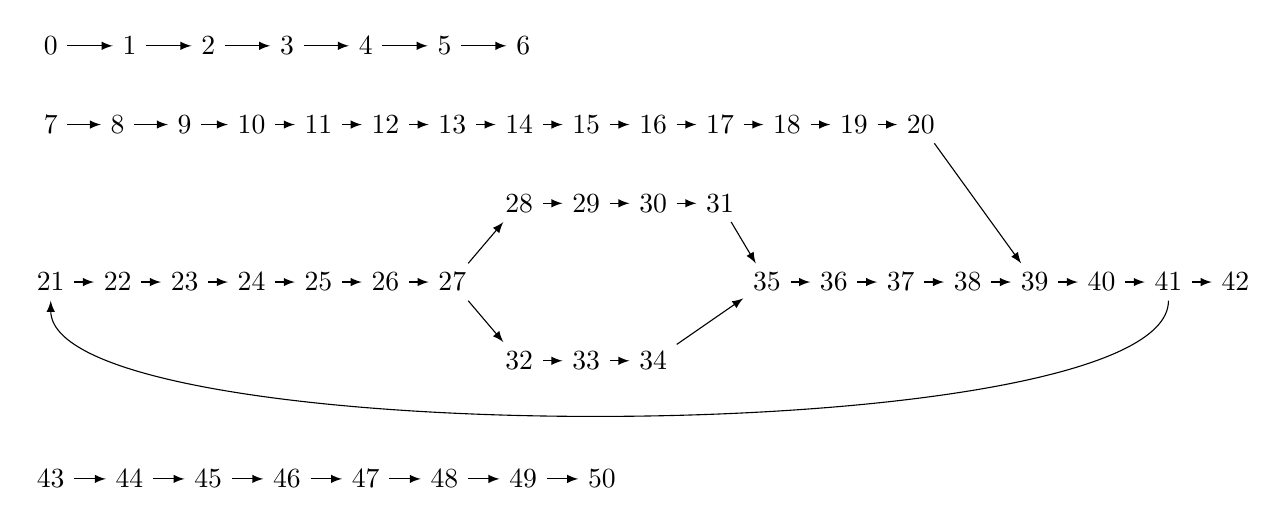
\begin{tikzpicture}[every new ->/.style={-latex}]
      % \node (start) at (0,0) {};
      \foreach \x in {0,...,6}  { \node (\x) at (\x, 1cm) {\x}; }
      \foreach \x in {7,...,20}  { \node (\x) at (0.85*\x - 0.85*7,0) {\x}; }
      \foreach \x in {21,...,27} { \node (\x) at (0.85*\x - 0.85*21, -2cm) {\x}; }
      \foreach \x in {28,...,31} { \node (\x) at (0.85*\x - 0.85*21, -1cm) {\x}; }
      \foreach \x in {32,...,34} { \node (\x) at (0.85*\x - 0.85*25, -3cm) {\x}; }
      \foreach \x in {35,...,42} { \node (\x) at (0.85*\x - 0.85*24.3, -2cm) {\x}; }
      \foreach \x in {43,...,50} { \node (\x) at (-43+\x, -4.5cm) {\x}; }

      \graph{ (7) -> (8) -> (9) -> (10) -> (11) -> (12) ->
        (13) -> (14) -> (15) -> (16) -> (17) -> (18) -> (19) -> (20)
        -> (39) -> (40) -> (41) -> (42); (21) -> (22) -> (23) -> (24)
        -> (25) -> (26) -> (27) -> {
          (28) -> (29) -> (30) -> (31);
          (32) -> (33) -> (34);
        } -> (35) -> (36) -> (37) -> (38) -> (39);
      };

      \graph{(0) -> (1) -> (2) -> (3) -> (4) -> (5) -> (6)};
      \graph{(43) -> (44) -> (45) -> (46) -> (47) -> (48) -> (49) -> (50)};

      \draw[-latex] (41) edge[out=270,in=270,looseness=0.35] (21);
    \end{tikzpicture}
  \end{center}
  \caption{Control flow graph for our example program}
  \label{example-control-flow-graph-figure}
\end{figure}

After the control flow graph is constructed, we consider each node in
turn, as specified by the for loop on
line~\ref{algorithm-sequence-cfg-loop}.
As mentioned earlier, we require a node to have only a single outgoing
edge and its target to have only a single incoming edge in order for
it to be considered for the introduction of sequential composition.
The reason for this is that nodes with two outgoing edges are points
at which conditionals should be introduced.
Such nodes in our example are the nodes for $pc$ values $27$ and $41$,
which represent the start of conditionals.
Likewise, nodes with multiple incoming edges represent points at which
a more complex control flows occur.
For our example, such nodes include $39$, which is the start of a
loop, and $35$, which is the end of a conditional.
These prevent introduction of sequential composition for the $pc$
values $20$, $31$, $34$, and $38$, since the targets of those nodes
are nodes $35$ and $39$.

For a node that meets the above requirement and is not a method call,
we can introduce sequential composition at that node by applying
Rule~[\nameref{sequence-introduction-rule}], on
line~\ref{algorithm-forward-sequence-application} of the algorithm.
This rule works by unrolling the loop in $Running$ to sequence an
instruction at $pc$ value $i$ with the instruction that is executed
after it, inserting $Poll$ inbetween.
It is required that the $pc$ value of the node's target, $j$, not be
the same as $i$, since that would introduce a loop, rather than a
sequential composition.
Also, the sequence of instructions at the node, $A$, must not affect
the non-emptiness of the $frameStack$ to ensure that the choice at the
start of the main loop in $Running$ can be resolved.
\begin{restatable}[sequence-intro]{crule}{SequenceIntroductionRule}
  \label{sequence-introduction-rule}
  Given $i : ProgramAddress$, if $i \neq j$ and \def\zedindent{0.25cm}
  \begin{circus}
    \{frameStack \neq \emptyset\} \circseq A \\
    {} = {} \\
    \{frameStack \neq \emptyset\} \circseq A \circseq \{frameStack \neq \emptyset\}
  \end{circus}
  then,
  \begin{circus}
    \begin{array}{l}
      \circmu X \circspot \\
      \t1 \circif frameStack = \emptyset \circthen \Skip \\
      \t1 {} \circelse frameStack \neq \emptyset \circthen {} \\
      \t2 \circif {} \cdots {} \\
      \t2 {} \circelse pc = i \circthen A \circseq pc := j \\
      \t2 {} \cdots {} \\
      \t2 {} \circelse pc = j \circthen B \\
      \t2 {} \cdots {} \\
      \t2 \circfi \circseq Poll \circseq X \\
      \t1 \circfi
    \end{array}
    \circrefines_A
    \begin{array}{l}
      \circmu X \circspot \\
      \t1 \circif frameStack = \emptyset \circthen \Skip \\
      \t1 {} \circelse frameStack \neq \emptyset \circthen {} \\
      \t2 \circif {} \cdots {} \\
      \t2 {} \circelse pc = i \circthen {} \\
      \t3 A \circseq pc := j \circseq Poll \circseq B \\
      \t2 {} \cdots {} \\
      \t2 {} \circelse pc = j \circthen B \\
      \t2 {} \cdots {} \\
      \t2 \circfi \circseq Poll \circseq X \\
      \t1 \circfi
    \end{array}
  \end{circus}
\end{restatable}

Since Rule~[\nameref{sequence-introduction-rule}] pulls two nodes
together, we can continue to introduce sequential composition at a
node after the first application of
Rule~[\nameref{sequence-introduction-rule}], until that node no longer
satisfies the conditions for introducing sequential composition.
This is specified by the while loop at
line~\ref{algorithm-forward-sequence-condition} of the algorithm.
This means the control flow graph is updated as
Rule~[\nameref{sequence-introduction-rule}] is applied, to take into
account the merging of nodes.
Since there are finitely many nodes, the merging of nodes eventually
results in a graph in which no further sequential compositions can be
introduced and so the loop terminates.

The resulting control flow graph after introduction of sequential
composition has been performed at every point is shown in
Figure~\ref{example-control-flow-graph-after-sequence-introduction-figure}.
We note that this graph is still a union of structured graphs since
merging sequentially composed nodes does not affect whether a graph is
structured.
This is due to the fact that sequential composition is one of the
constructs used to define structured control flow graphs
(Figure~\ref{sequence-figure}), and merging the nodes may be seen as
performing the reverse of node replacement for it.
\begin{figure}
  \begin{center}
    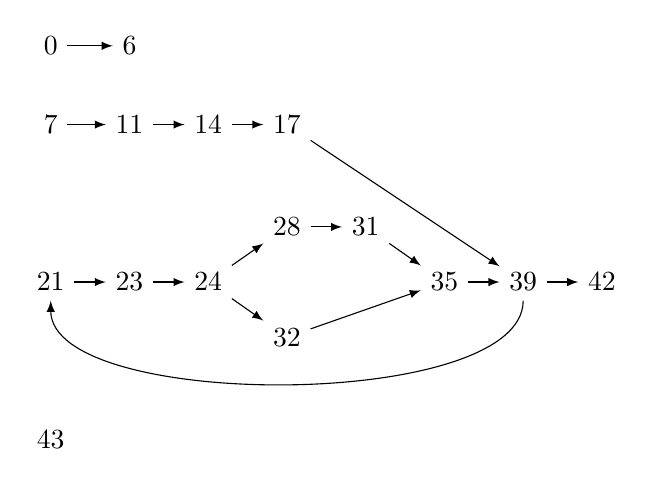
\begin{tikzpicture}[every new ->/.style={-latex}]
      \path (0,0) node (0) {0} -- ++(1,0) node (6) {6};
      \path (0,-1cm) node (7) {7} -- ++(1,0) node (11) {11} -- ++(1,0) node (14) {14} -- ++(1,0) node (17) {17};
      \path (0,-3cm) node (21) {21} -- ++(1,0) node (23) {23} -- ++(1,0) node (24) {24};
      \path (3,-2.3cm) node (28) {28} -- ++(1,0) node (31) {31};
      \node at (3,-3.7cm) (32) {32};
      \path (5,-3cm) node (35) {35} -- ++(1,0) node (39) {39} -- ++(1,0) node (42) {42};
      
      \graph{
        (7) -> (11) -> (14) -> (17) -> (39) -> (42);
        (21) -> (23) -> (24) -> {
          (28) -> (31);
          (32);
        } -> (35) -> (39);
      };

      \graph[grow down]{(0) -> (6)};
      \node at (0,-5cm) {43};

      \draw[-latex] (39) edge[out=270,in=270,looseness=0.6] (21);
    \end{tikzpicture}
  \end{center}
  \caption{Control flow graph for our example after sequential composition introduction}
  \label{example-control-flow-graph-after-sequence-introduction-figure}
\end{figure}

The only remaining nodes in this graph are those where the sequence of
instructions ends with a method call or return, or which represent a
more complex control flow.
In particular, the instructions for the \texttt{f()} method of
\texttt{TPK}, which begin at $pc = 43$, have been completely sequenced
together into a single node.
The code that corresponds to this control flow graph is that shown
earlier in Figure~\ref{forward-sequence-introduction-example-figure}.

\subsection{Introduce Loops and Conditionals}
\label{introduce-loops-and-conditionals-subsection}

After sequential composition has been introduced for all methods, we
must consider each method separately to handle method calls.
This means the strategy must loop, introducing loops and conditionals
to those methods that have no unresolved method calls and resolving
calls of methods that are then complete, until every method is
complete and has been separated into its own action.

Introducing loops and conditionals is performed as described by
Algorithm~\ref{introduce-loops-and-conditionals-algorithm}.
This considers each method individually, as specified by the for loop
on line~\ref{algorithm-introduce-loops-and-conditionals-method-loop}
of the algorithm. 
The condition on line~\ref{algorithm-no-unresolved-calls-condition}
ensures that only those methods where all method calls have already
been resolved undergo loop and conditional introduction.
Since we do not allow recursion, there is always at least one method
that does not depend on another method in the program.
It may be the case that a method depends only on special methods, in
which case this stage has no effect on that method until the special
method calls have been resolved.
Special method calls can always be resolved as they do not depend on
other methods in the program.

The \Call{HasNoUresolvedCalls}{$m$} procedure, used in the condition
on line~\ref{algorithm-no-unresolved-calls-condition}, checks that no
node in the control flow graph of $m$ ends in a method call, as a way
of determining whether $m$ has unresolved calls.
Since method resolution sequences a method call with the instructions
following it, a method call with nothing following it is a call that
has not yet been resolved.

\begin{algorithm}
  \begin{algorithmic}[1]
    \For{$m \gets methods$}
    \label{algorithm-introduce-loops-and-conditionals-method-loop}
    \If{\Call{HasNoUresolvedCalls}{$m$}}
    \label{algorithm-no-unresolved-calls-condition}
    \State $cfg \gets$ \Call{MakeMethodControlFlowGraph}{$m$}
    \label{algorithm-make-control-flow-graph2}
    \For{$node \gets$ \Call{ReverseNodes}{$cfg$}}
    \label{algorithm-node-checking-loop}
    \State \ApplyFor{Rule~[\nameref{if-introduction-rule}]}{$node$}
    \label{algorithm-introduce-if}
    \State \ApplyFor{Rule~[\nameref{if-else-introduction-rule}]}{$node$}
    \label{algorithm-introduce-if-else}
    \If{\Call{IsSimpleConditional}{$node$}}
    \label{algorithm-conditional-check}
    \State \ApplyFor{Rule~[\nameref{conditional-introduction-rule}]}{$node$}
    \label{algorithm-introduce-conditional}
    \EndIf
    \State \ApplyFor{Rule~[\nameref{while-introduction-rule1}]}{$node$}
    \label{algorithm-introduce-while1}
    \State \ApplyFor{Rule~[\nameref{while-introduction-rule2}]}{$node$}
    \label{algorithm-introduce-while2}
    \State \ApplyFor{Rule~[\nameref{do-while-introduction-rule}]}{$node$}
    \label{algorithm-introduce-do-while}
    \State \ApplyFor{Rule~[\nameref{infinite-loop-introduction-rule}]}{$node$}
    \label{algorithm-introduce-infinite-loop}
    \If{\Call{HasSimpleSequence}{$node$}}
    \label{algorithm-lci-sequence-check}
    \State \ApplyFor{Rule~[\nameref{sequence-introduction-rule}]}{$node$}
    \label{algorithm-lci-sequence-introduction}
    \EndIf
    \EndFor
    \EndIf
    \EndFor
  \end{algorithmic}
  \caption{IntroduceLoopsAndConditionals}
  \label{introduce-loops-and-conditionals-algorithm}
\end{algorithm}

For each method that undergoes loop and conditional introduction, we
consider again its control-flow graph to ensure the loops and
conditionals are introduced in the correct order to properly form
their bodies.
This involves constructing a control-flow graph for the method, at
line~\ref{algorithm-make-control-flow-graph2}.
The control-flow graph for a method $m$ is created by the procedure
\Call{MakeMethodControlFlowGraph}{$m$}.
This is similar to the \Call{MakeControlFlowGraph}{} procedure used in
the previous section, but it just constructs the graph
for a single method, starting at the entry point of that method.

The graph for the \texttt{handleAsyncEvent()} method in our example
(beginning at $pc=7$, its entry point) is shown in
Figure~\ref{example-simplified-control-flow-graph-figure}, alongside
the \Circus{} code obtained at the beginning of this stage for the
method.
The edge that forms a loop from $pc=35$ to $pc=39$ is shown as a
dashed line since looping edges are ignored at certain points in this
part of the strategy.
\begin{figure}
  \begin{center}
    % \begin{multicols}{4}
    \begin{minipage}{0.3\linewidth}
      \begin{tikzpicture}
        \node (7)  at (0,0)  {7};
        \node (39)  at (0,-1) {39};
        \node (42) at (-1,-2) {42};
        \node (21) at (1,-2) {21};
        \node (28) at (0.5,-3) {28};
        \node (32) at (1.5,-3) {32};
        \node (35) at (1,-4) {35};
        \draw[-latex] (7) to (39);
        \draw[-latex] (39) to (42);
        \draw[-latex] (39) to (21);
        \draw[-latex] (21) to (28);
        \draw[-latex] (21) to (32);
        \draw[-latex] (28) to (35);
        \draw[-latex] (32) to (35);
        % \draw[-latex,red!70!black,dashed,out=0,in=0,looseness=1.1] (35) to (39);
        \draw[-latex,dashed,out=0,in=0,looseness=1.1] (35) to (39);
      \end{tikzpicture}
    \end{minipage}
    % \columnbreak
    \begin{minipage}{0.6\linewidth}
      \scriptsize
      \setlength{\zedindent}{0cm}
      \begin{circus}
        Running \circdef \\
        \t1 \circif frameStack = \emptyset \circthen \Skip \\
        \t1 {} \circelse frameStack \neq \emptyset \circthen {} \\
        \t2 \circif pc = 0 \circthen {} \cdots {} \\
        \t2 {} \circelse pc = 7 \circthen HandleNewEPC(27) \circseq pc := 8 \circseq Poll \circseq \cdots \circseq \\
        \t3 pc := 39 \\
        \t2 {} \cdots {} \\
        \t2 {} \circelse pc = 21 \circthen HandleAloadEPC(2) \circseq pc := 22 \circseq Poll \circseq \cdots \circseq \\
        \t3 pc := \IF value1 \leq value2 \THEN 32 \ELSE 28 \\
        \t2 {} \cdots {} \\
        \t2 {} \circelse pc = 28 \circthen HandleAloadEPC(3) \circseq pc := 29 \circseq Poll \circseq \cdots \circseq \\
        \t3 pc := 35 \\
        \t2 {} \cdots {} \\
        \t2 {} \circelse pc = 32 \circthen HandleAloadEPC(3) \circseq pc := 33 \circseq Poll \circseq \cdots \circseq \\
        \t3 pc := 35 \\
        \t2 {} \cdots {} \\
        \t2 {} \circelse pc = 35 \circthen HandleAloadEPC(4) \circseq pc := 36 \circseq Poll \circseq \cdots \circseq \\
        \t3 pc := 39 \\
        \t2 {} \cdots {} \\
        \t2 {} \circelse pc = 39 \circthen HandleAloadEPC(4) \circseq pc := 36 \circseq Poll \circseq \cdots \circseq \\
        \t3 pc := \IF value1 \leq value2 \THEN 21 \ELSE 42 \\
        \t2 {} \cdots {} \\
        \t2 {} \circelse pc = 42 \circthen HandleReturnEPC \\
        \t2 \circfi \circseq Poll \circseq Running \\
        \t1 \circfi
      \end{circus}
    \end{minipage}
    %\end{multicols}
  \end{center}
  \caption{Simplified control flow graph and corresponding code for our example
    program}
  \label{example-simplified-control-flow-graph-figure}
\end{figure}

%TODO: explain how our definition of structure differs from that of
% MISRA - leave for final considerations?

The control-flow graph of each method is structured since the
transformations of the graph up to this point consist solely of
collapsing sequential compositions, which, as mentioned in the
previous section, does not cause a structured graph to become
unstructured.
Since we have defined the desired program structure in terms of a
small number of standard structures (shown in
Figure~\ref{structured-cfg-figures}), we can identify each of these
structures in the graph and introduce them into the program,
collapsing the graph in the process.

In order to easily identify the structures in isolation from other
structures, we begin at the end nodes of the method (ignoring looping
edges for the purposes of determining end nodes) and work backwards,
considering each node in turn.
This is specified by the loop beginning on
line~\ref{algorithm-node-checking-loop} of
Algorithm~\ref{introduce-loops-and-conditionals-algorithm}.
% TODO: ReverseNodes should return a sequence and should be more
% carefully defined
The procedure \Call{ReverseNodes}{$cfg$} iterates over the nodes of
$cfg$ beginning at the end nodes and moving in the reverse direction
of the graph edges, ignoring looping edges.
In our example this means we consider the $pc=42$ and $pc=35$ nodes
first, then $pc=28$ and $pc=32$, then $pc=21$, $pc=39$, and finally
$pc=7$.

For each node, we check each type of structure to see if the
control-flow graph starting at that point matches the structure, and
introduce the structure if it does.
Some of the structures (Figure~\ref{if-figure},
\subref{if-else-figure}, \subref{while-figure} and
\subref{do-while-figure}) are followed by further instructions.
A sequential composition must be introduced with the instructions
following the structure.
However, in programs with graphs such as the one shown below, the
sequential composition can only be introduced after the outer
conditional has been introduced.
Thus, the introduction of the sequential composition cannot be made
part of the rule for introducing the conditional.
\begin{center}
  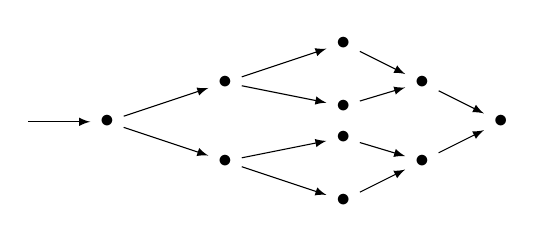
\begin{tikzpicture}
    \node (1) at (0.0, 0.0) {$\bullet$};
    \node (2) at (1.5, 0.5) {$\bullet$};
    \node (3) at (1.5,-0.5) {$\bullet$};
    \node (4) at (3.0, 1.0) {$\bullet$};
    \node (5) at (3.0,-1.0) {$\bullet$};
    \node (6) at (3.0, 0.2) {$\bullet$};
    \node (7) at (3.0,-0.2) {$\bullet$};
    \node (8) at (4.0, 0.5) {$\bullet$};
    \node (9) at (4.0,-0.5) {$\bullet$};
    \node (0) at (5.0, 0.0) {$\bullet$};
    
    \draw[-latex] (-1,0) to (1);
    
    \draw[-latex] (1) to (2);
    \draw[-latex] (1) to (3);
    \draw[-latex] (2) to (4);
    \draw[-latex] (3) to (5);
    \draw[-latex] (2) to (6);
    \draw[-latex] (3) to (7);
    \draw[-latex] (4) to (8);
    \draw[-latex] (5) to (9);
    \draw[-latex] (6) to (8);
    \draw[-latex] (7) to (9);
    \draw[-latex] (8) to (0);
    \draw[-latex] (9) to (0);
  \end{tikzpicture}
\end{center}

The first type of structure we check for are conditionals.
There are three conditional structures:~\texttt{if} conditionals
(Figure~\ref{if-figure}), \texttt{if}-\texttt{else} conditionals
(Figure~\ref{if-else-figure}), and divergent conditionals
(Figure~\ref{divergent-figure}).
We introduce each with a separate rule, specialised to the form of the
conditional.

An \texttt{if} conditional with no else branch is introduced using
Rule~[\nameref{if-introduction-rule}], shown below.
Such a structure can be recognised from the form of the \Circus{} code
in the $Running$ action, which is that of a node whose sequence of
instructions ends with an assignment of the form
$pc := \IF b \THEN x \ELSE y$, and for which the $pc = y$ node ends in
an assignment $pc := x$.
Note that the branches cannot be the other way round (i.e.\ the
$pc = x$ branch will not be the body of the conditional) since the
conditional branches come from Java's branching instructions, which
branch to the specified address if the condition is true and go to the
next instruction if it is false.
\begin{restatable}[\texttt{if}-conditional-intro]{crule}{IfConditionalIntroductionRule}
  \label{if-introduction-rule}
  \setlength{\zedindent}{0.25cm}
  % \setlength{\abovedisplayskip}{0.1cm}
  % \setlength{\belowdisplayskip}{0.1cm}
  Given $i : ProgramAddress$, if $i \neq j$, $i \neq k$, and 
  \begin{circus}
    \{frameStack \neq \emptyset\} \circseq A \\
    {} = {} \\
    \{frameStack \neq \emptyset\} \circseq A \circseq \{frameStack \neq \emptyset\}
  \end{circus}
  then
  \begin{circus}
    \begin{array}{l}
      \circmu X \circspot \\
      \t1 \circif frameStack = \emptyset \circthen \Skip \\
      \t1 {} \circelse frameStack \neq \emptyset \circthen {} \\
      \t2 \circif \cdots \\
      \t2 {} \circelse pc = i \circthen A \circseq \\
      \t3 pc := \IF b \THEN j \ELSE k \\
      \t2 {} \cdots {} \\
      \t2 {} \circelse pc = k \circthen B \circseq pc := j \\
      \t2 {} \cdots {} \\
      \t2 \circfi \circseq Poll \circseq X \\
      \t1 \circfi
    \end{array}
    \circrefines_A
    \begin{array}{l}
      \circmu X \circspot \\
      \t1 \circif frameStack = \emptyset \circthen \Skip \\
      \t1 {} \circelse frameStack \neq \emptyset \circthen {} \\
      \t2 \circif \cdots \\
      \t2 {} \circelse pc = i \circthen A \circseq \\
      \t3 \circif b \circthen \Skip \\
      \t3 {} \circelse \lnot b \circthen pc := k \circseq Poll \circseq B \\
      \t3 \circfi \circseq pc := j \\
      \t2 {} \cdots {} \\
      \t2 {} \circelse pc = k \circthen B \circseq pc := j \\
      \t2 {} \cdots {} \\
      \t2 \circfi \circseq Poll \circseq X \\
      \t1 \circfi 
    \end{array}
  \end{circus}
\end{restatable}
Rule~[\nameref{if-introduction-rule}] introduces a conditional for
nodes that match the form described above, which in the rule is the
$pc = i$ node.
The conditional is introduced with the true branch empty (represented
by $\Skip$) and the false branch containing the instructions in the
body of the conditional.
The assignment $pc := j$ is moved outside the conditional from both
the true amd false branches.

As in Rule~[\nameref{sequence-introduction-rule}], the sequence of
actions for the node must not affect the nonemptiness of the
$frameStack$.
A similar condition is required for all the rules in this section.
We also require that the targets of the conditional are different from
the node at which the conditional is introduced, since that would
introduce a loop, which is not the purpose of this rule.
Rule~[\nameref{if-introduction-rule}] is applied on
line~\ref{algorithm-introduce-if} of
Algorithm~\ref{introduce-loops-and-conditionals-algorithm}.
Note that, since the structure can be identified from the form of the
\Circus{} code alone, it is not necessary to guard the application of
the rule with a condition on the control-flow graph.

We introduce \texttt{if}-\texttt{else} conditionals using
Rule~[\nameref{if-else-introduction-rule}] and divergent conditionals
using Rule~[\nameref{conditional-introduction-rule}].
Since these are similar to Rule~[\nameref{if-introduction-rule}], we
omit them here.
They can be found in Appendix~\ref{compilation-rules-appendix}.
We apply these rules on lines~\ref{algorithm-introduce-if-else}
and~\ref{algorithm-introduce-conditional}.

Rule~[\nameref{conditional-introduction-rule}] introduces a
conditional with no restrictions on its form.
To ensure it is only applied to nodes that match the form of
Figure~\ref{divergent-figure}, we guard its application by the
condition \Call{IsSimpleConditional}{$node$} on
line~\ref{algorithm-conditional-check}.
The procedure \Call{IsSimpleConditional}{$node$} checks if the targets
of $node$ have no outgoing nodes.
This is a condition on the control-flow graph that cannot be expressed
in the statement of the rule.

After attempting to introduce conditionals, we attempt to introduce
loops.
There are three types of loop to consider, as shown earlier:
\texttt{while} loops (Figure~\ref{while-figure}),
\texttt{do}-\texttt{while} loops (Figure~\ref{do-while-figure}), and
infinite loops (Figure~\ref{infinite-loop-figure}).
A \texttt{while} loop has a form similar to that of a conditional,
except that one of the branches ends with a jump back to the beginning
of the node with the conditional.
This structure may be introduced using
Rule~[\nameref{while-introduction-rule1}] below.
This rule introduces a conditional at a node $pc=i$ with its false
branch ending in an assignment of $i$ to $pc$, and introduces a
recursion to the beginning of the $pc=i$ node in that branch of the
conditional, representing a loop.
Since this loop may be within a conditional, we simply move the $pc$
assignment for the true branch outside the conditional, so that a
sequential composition can be introduced later, as with \texttt{if}
and \texttt{if}-\texttt{else} conditionals.
\begin{restatable}[\texttt{while}-loop-intro1]{crule}{WhileLoopIntroductionRuleA}
  \label{while-introduction-rule1}
  \setlength{\zedindent}{0.2cm}
  \setlength{\zedtab}{0.9\zedtab}
  Given $i : ProgramAddress$, if $i \neq j$,
  \begin{circus}
    \{frameStack \neq \emptyset\} \circseq A \\
    {} = {} \\
    \{frameStack \neq \emptyset\} \circseq A \circseq \{frameStack \neq \emptyset\}
  \end{circus}
  then
  \begin{circus}
    \begin{array}{l}
      \circmu X \circspot \\
      \t1 \circif frameStack = \emptyset \circthen \Skip \\
      \t1 {} \circelse frameStack \neq \emptyset \circthen {} \\
      \t2 \circif \cdots \\
      \t2 {} \circelse pc = i \circthen A \circseq \\
      \t3 pc := \IF b \THEN j \ELSE k \\
      \t2 \cdots \\
      \t2 {} \circelse pc = j \circthen B \\
      \t2 \cdots \\
      \t2 {} \circelse pc = k \circthen C \circseq pc := i \\
      \t2 \cdots \\
      \t2 \circfi \circseq Poll \circseq X \\
      \t1 \circfi 
    \end{array}
    \circrefines_A
    \begin{array}{l}
      \circmu X \circspot \\
      \t1 \circif frameStack = \emptyset \circthen \Skip \\
      \t1 {} \circelse frameStack \neq \emptyset \circthen {} \\
      \t2 \circif \cdots \\
      \t2 {} \circelse pc = i \circthen (\circmu Y \circspot A \circseq \\
      \t3 \circif b \circthen \Skip \\
      \t3 {} \circelse \lnot b \circthen {} \\
      \t4 pc := k \circseq Poll \circseq C \circseq pc := i \circseq Poll \circseq Y \\
      \t3 \circfi) \circseq pc := j \\
      \t2 \cdots \\
      \t2 {} \circelse pc = j \circthen B \\
      \t2 \cdots \\
      \t2 {} \circelse pc = k \circthen C \circseq pc := i \\
      \t2 \cdots \\
      \t2 \circfi \circseq Poll \circseq X \\
      \t1 \circfi 
    \end{array}
  \end{circus}
\end{restatable}%
As a \texttt{while} loop may occur with the loop at the end of either
condition branch (since the loop may be created by a \texttt{goto}
instruction in the Java bytecode), we also provide a similar rule,
Rule~[\nameref{while-introduction-rule2}], which introduces the loop
in the true branch of the conditional.
These two rules are applied on lines~\ref{algorithm-introduce-while1}
and~\ref{algorithm-introduce-while2} of the algorithm.
Rule~[\nameref{while-introduction-rule2}] is presented in
Appendix~\ref{compilation-rules-appendix}.

The second type of loop we introduce is the \texttt{do}-\texttt{while}
loop.
A \texttt{do}-\texttt{while} loop is similar to a \texttt{while} loop,
but is distinguished by the fact that the conditional $pc$ assignment
that causes the loop is at the end of the loop, rather than at the
beginning or in the middle.
We introduce these loops using
Rule~[\nameref{do-while-introduction-rule}], which we omit due to its
similarity with Rule~[\nameref{while-introduction-rule1}]; it is
presented in Appendix~\ref{compilation-rules-appendix}.
This rule is applied on line~\ref{algorithm-introduce-do-while} of the
algorithm.
Note that the false branch can never cause the loop in this case,
since it will just go to the next instruction.
Attempting to redirect it and create the loop with a \texttt{goto}
instruction would add an instruction within the loop after the
conditional, so it would be dealt with as a \texttt{while} loop.
Therefore, it is not necessary to provide two compilation rules for
\texttt{do}-\texttt{while} loops, unlike \texttt{while} loops where

The final loop structure that we attempt to introduce is that of an
infinite loop.
An infinite loop may be identified as a block of instructions that
ends with a $pc$ assignment that causes a jump back to the beginning
of the block of instructions.
We introduce these loops using
Rule~[\nameref{infinite-loop-introduction-rule}], presented in
Appendix~\ref{compilation-rules-appendix}.
This rule is applied on line~\ref{algorithm-introduce-infinite-loop}
of the algorithm.

After we have attempted to introduce each of the structures for a
particular node, we attempt to introduce a sequential composition.
This ensures that \texttt{if}, \texttt{if}-\texttt{else},
\texttt{while} and \texttt{do}-\texttt{while} structures that occur
within conditionals are sequentially composed with the node following
them if possible.
It also handles cases where sequential compositions occur before
loops, preventing them from being introduced in
Section~\ref{introduce-forward-sequence-subsection} without
interfering with the introduction of the loop.
Such a case occurs at the $pc=7$ node in our example.

The requirement for sequential composition to be introduced is the
same as in Section~\ref{introduce-forward-sequence-subsection}:~it
must be a simple sequential composition from a node with a single
outgoing edge to a node with a single incoming edge.
Thus we check for a simple sequence on
line~\ref{algorithm-lci-sequence-check} of
Algorithm~\ref{introduce-loops-and-conditionals-algorithm}.
The sequential composition is then introduced on
line~\ref{algorithm-lci-sequence-introduction} if it is a simple
sequential composition.

As mentioned earlier, these steps are repeated for each node, working
backwards through the control-flow graph of each method.
Each of the rules for introducing control flow structures reduces the
graph to either a sequential composition graph
(Figure~\ref{sequence-figure}) or a single node.
Divergent conditionals and infinite loops are the structures whose
control-flow graphs are reduced to a single node by their introduction
rules.

The remaining structures are reduced to sequential composition graphs.
The reduction of the seqential composition graph depends on which form
of node replacement is used to embed the structure in the control-flow
graph of the method.
There are four cases to consider:~root-node replacement
(Figure~\ref{root-replacement-figure}), end-node replacement
(Figure~\ref{end-replacement-figure}), internal-node replacement
(Figure~\ref{internal-replacement-figure}) and branch-end replacement
(Figure~\ref{branch-end-replacement-figure}).
Replacing the root node of a
graph $G$ with a graph $H$ can be viewed as replacing the end node of
$H$ with $G$.
Since we are considering the nodes moving backwards through the
control flow graph, we will always treat this as an end node
replacement.

In the cases of end-node replacement and internal-node replacement we
can introduce the sequential composition immediately, reducing the
graph to a single node.
In the case of branch-end replacement, if some graph $H$ is embedded
in a graph $G$, then reducing $H$ to a sequential composition results
in the overall graph having the form of $G$.
This can be seen from the example shown in
Figure~\ref{branch-end-replacement-figure}, where reducing the
\texttt{while} loop structure formed by nodes $a$, $b$ and $4$ to a
sequential composition yields the graph shown in
Figure~\ref{branch-end-reduction-figure}.
This has the form of a \texttt{if}-\texttt{else} conditional
(Figure~\ref{if-else-figure}).
Such structures are introduced on further iterations of the loop over
the nodes.
Thus, given a structured control flow graph at the beginning of this
stage, the control flow graph is reduced to a single node, with all
the control flow structures in the method introduced.

\begin{figure}
  \begin{center}
    \begin{tikzpicture}
      \useasboundingbox (-1.5,-2.5) rectangle (1.5,2);
      \node at (0,2) (start) {};
      \node at ( 0, 1)    (A) {$1$};
      \node at (-1,-0.5)  (B) {$a$};
      \node at ( 1,-0.5)  (C) {$3$};
      %\node at (-2,-1.5)  (D) {$b$};
      \node at ( 0,-2)    (G) {$4$};
      \draw[-latex] (start) -- (A);
      \draw[-latex] (A) -- (B);
      \draw[-latex] (A) -- (C);
      %\draw[-latex] (B) to (D);
      \draw[-latex] (B) to (G);
      %\draw[-latex] (D) to[in=180,out=90] (B);
      \draw[-latex] (C) -- (G);
    \end{tikzpicture}
  \end{center}
  \caption{The graph of Figure~\ref{branch-end-replacement-figure} after loop introduction}
  \label{branch-end-reduction-figure}
\end{figure}

In our example, we begin at the $pc=35$ node, where there are no
structures to introduce. 
The same holds true of the $pc=28$ and $pc=32$ nodes (note that the
edges coming from them are not simple sequential compositions).
An \texttt{if}-\texttt{else} conditional is introduced at $pc=21$,
absorbing the $pc=28$ and $pc=32$ nodes.
The sequential composition from the $pc=21$ node to the $pc=35$ node
can then be introduced immediately as it is now a simple sequential
composition (because it is not at the end of an outer conditional).
We then introduce a \texttt{while} loop at the $pc=39$ loop (using
Rule~[\nameref{while-introduction-rule2}]), and the sequential
composition with the $pc=42$ node is introduced afterwards.
Finally, a sequential composition from the $pc=7$ to the $pc=39$ node
is introduced, collapsing the control flow graph to a single node.
The code at $pc=7$ is then that shown earlier in
Figure~\ref{loop-and-conditional-introduction-example-figure}.

\subsection{Resolve Method Calls}
\label{resolve-method-calls-subsection}

When a method is complete, calls to that method can then be resolved.
This step begins with the copying of the method into a separate
action, so that it can be referenced elsewhere.
This is performed as described by
Algorithm~\ref{separate-complete-methods-algorithm}.
\begin{algorithm}
  \begin{algorithmic}[1]
    \For{$m \gets methods$} \label{algorithm-method-separation-loop}
    \If{\Call{MethodIsComplete}{$m$}} \label{algorithm-check-method-completeness}
    \State \ApplyFor{Rule~[\nameref{introduce-class-information-rule}]}{$m$}
    \label{algorithm-introduce-class-information}
    \State \ApplyFor{Law~[\nameref{action-intro-law}]}{$m$} \label{algorithm-introduce-method-action}
    \State \ApplyFor{Law~[\nameref{copy-rule-law}]}{$m$} \label{algorithm-copy-method-action}
    \EndIf
    \EndFor
  \end{algorithmic}
  \caption{SeparateCompleteMethods}
  \label{separate-complete-methods-algorithm}
\end{algorithm}

Algorithm~\ref{separate-complete-methods-algorithm} looks at each
method separately, as specified by the loop on
line~\ref{algorithm-method-separation-loop}, and determines if it is
complete, on line~\ref{algorithm-check-method-completeness}.
This involves a simple syntactic check that each conditional branch
ends in a return instruction or a recursion.

If a method is complete, we first introduce an assumption at the start
of the sequence of actions for the method that establishes what the
value of $currentClass$ is during the method's execution
(line~\ref{algorithm-introduce-class-information}).
This is performed by an application of
Rule~[\nameref{introduce-class-information-rule}], shown in
Figure~\ref{introduce-class-information-rule-figure}.
The $currentClass$ is determined by finding the class information $c$
in the range of $cs$ that contains a method $m$ with the same entry
point, $i$, as the complete method being operated on.
By recording this information in an assumption, we can use it in later
stages of the compilation, when the value of the $pc$ is no longer
available.
\begin{figure}
\begin{restatable}[introduce-class-information]{crule}{IntroduceClassInformationRule}
  \label{introduce-class-information-rule}
  Given $i : ProgramAddress$,
  \begin{circus}
    \begin{array}{l}
      \circmu X \circspot \\
      \t1 \circif frameStack = \emptyset \circthen \Skip \\
      \t1 {} \circelse frameStack \neq \emptyset \circthen {} \\
      \t2 \circif \cdots \\
      \t2 {} \circelse pc = i \circthen A \\
      \t2 {} \cdots {} \\
      \t2 \circfi \circseq Poll \circseq X \\
      \t1 \circfi
    \end{array}
    \circrefines_A
    \begin{array}{l}
      \circmu X \circspot \\
      \t1 \circif frameStack = \emptyset \circthen \Skip \\
      \t1 {} \circelse frameStack \neq \emptyset \circthen {} \\
      \t2 \circif \cdots \\
      \t2 {} \circelse pc = i \circthen \{currentClass = c\} \circseq A \\
      \t2 {} \cdots {} \\
      \t2 \circfi \circseq Poll \circseq X \\
      \t1 \circfi
    \end{array}
  \end{circus}
  where $c : Class$ is such that
  \begin{displaymath}
    c \in \ran cs \land \exists  m : MethodID | m \in \dom c.methodEntry @ c.methodEntry~m = i.
  \end{displaymath}
\end{restatable}
\caption{Rule~[\nameref{introduce-class-information-rule}]}
\label{introduce-class-information-rule-figure}
\end{figure}

For the methods that are complete, the sequence of actions for the
method are placed in a separate action, which is introduced using
Law~[\nameref{action-intro-law}] on
line~\ref{algorithm-introduce-method-action}.
We form the name of this action from the name of the class to which
the method belongs and the name of the method, concatenated together
with an underscore.
This is similar to how icecap forms method names, although the name
used for the action does not have an effect upon the correctness of
the strategy, provided it is unique.
Once the method action has been introduced, the sequence of actions at
the method's entry point in the $Running$ action is replaced with a
reference to the newly introduced action by applying
Law~[\nameref{copy-rule-law}] on
line~\ref{algorithm-copy-method-action}.

In our example, the method \texttt{f()} of the \texttt{TPK} class,
which starts at $pc = 43$, is complete on the first iteration of the
loop on line~\ref{algorithm-method-loop} of
Algorithm~\ref{epc-algorithm}.
This can be seen in
Figure~\ref{forward-sequence-introduction-example-figure}.
The method is complete in this case because it consists of a straight
sequence of instructions ending with $HandleAreturnEPC$, which
represents the \texttt{areturn} instruction.
The sequence of instructions at $pc = 43$ is copied into the action $TPK\_f$,
which can be seen in
Figure~\ref{method-call-resolution-example-figure}.
The $pc = 43$ branch is replaced with a call to $TPK\_f$.

After all the complete methods have been copied into separate actions,
calls to those methods are resolved.
This is performed as described by
Algorithm~\ref{resolve-method-calls-algorithm}.
In this algorithm, while we indicate the parameters supplied to a rule
with the word \textbf{for}, as in previous algorithms, we use the word
\textbf{to} to indicate which part of the $Running$ action the rule is
applied to.
In all previous algorithms, the laws are applied to the whole action,
and so we omit the \textbf{to} clause.
\begin{algorithm}[th]
  \begin{algorithmic}[1]
    \For{$m \gets methods$}
    \label{algorithm-mci-method-loop} 
    \For{$mc \gets$ \Call{UnresolvedMethodsCalls}{$m$}}
    \label{algorithm-mci-method-call-loop}
    \If{\Call{IsResolvable}{$mc$}}
    \label{algorithm-is-resolvable-check}
    \If{\Call{HasSingleTarget}{$mc$}}
    \label{algorithm-multiple-targets-check}
    \Try
    \label{algorithm-try-block-begin}
    \State \ApplyTo{Rule~[\nameref{refine-invokespecial-rule}]}{$mc$}
    \State \ApplyTo{Rule~[\nameref{refine-invokestatic-rule}]}{$mc$}
    \State \ApplyTo{Rule~[\nameref{refine-invokevirtual-single-rule}]}{$mc$}
    \EndTry
    \Try
    \label{algorithm-try-block2-start}
    \State \ApplyTo{Rule~[\nameref{resolve-special-method-rule}]}{$mc$}
    \State \ApplyTo{Rule~[\nameref{resolve-special-method-virtual-rule}]}{$mc$}
    \State \ApplyFor{Rule~[\nameref{resolve-normal-method-rule}]}{$mc$}
    \State \ApplyFor{Rule~[\nameref{resolve-normal-method-virtual-rule}]}{$mc$}
    \EndTry
    \Else
    \State \ApplyTo{Rule~[\nameref{refine-invokevirtual-multi-rule}]}{$mc$}
    \label{algorithm-refine-invokevirtual-multi}
    \For{$target \gets $\Call{Targets}{$mc$}}
    \label{algorithm-targets-loop}
    \Try
    \State \ApplyToFor{Rule~[\nameref{resolve-special-method-branch-rule}]}{$mc$}{$target$}
    \State \ApplyFor{Rule~[\nameref{resolve-normal-method-branch-rule}]}{$mc$, $target$}
    \EndTry
    \EndFor
    \State \ApplyFor{Law~[\nameref{alt-seq-dist-law}]}{$mc$}
    \label{algorithm-move-pc-assignments}
    \EndIf
    \If{\Call{HasSimpleSequence}{$node$}}
    \label{algorithm-mci-sequence-introduction-start}
    \State \ApplyFor{Rule~[\nameref{sequence-introduction-rule}]}{$node$}
    \EndIf
    \label{algorithm-mci-sequence-introduction-end}
    \EndIf
    \EndFor
    \EndFor
  \end{algorithmic}
  \caption{ResolveMethodCalls}
  \label{resolve-method-calls-algorithm}
\end{algorithm}

The algorithm begins by checking each unresolved method call in each
method, as specified by the loops on
lines~\ref{algorithm-mci-method-loop}
and~\ref{algorithm-mci-method-call-loop}.
The list of unresolved method calls for a given method, $m$, is
computed by \Call{UnresolvedMethodsCalls}{$m$}, which finds the $pc$
values for which the sequence of instructions ends with a method
invocation instruction with no $pc$ assignment following it.
An example of an unresolved method call can be seen in the $pc = 14$
branch of Figure~\ref{forward-sequence-introduction-example-figure},
reproduced in part below.
\begin{circusaction}
  \t2 {} \cdots {} \\
  \t2 {} \circelse pc = 14 \circthen \cdots \circseq pc := 16 \circseq Poll \circseq HandleInvokevirtualEPC(36) \\
  \t2 {} \cdots {}
\end{circusaction}
This ends with the action $HandleInvokeVirtualEPC(36)$, which handles
the \texttt{invokevirtual} instruction for the constant pool index
$36$.
It is unresolved because it does not have any $pc$ assignment or other
actions following it.

For each method call that needs resolving, we check if it can be
resolved at this point in the compilation strategy.
This is performed on line~\ref{algorithm-is-resolvable-check}, where
the boolean value \Call{IsResolvable}{$mc$} is checked.
\Call{IsResolvable}{$mc$} is true if all the targets of the method
call $mc$ are either special methods or non-special methods that are
already complete and have been separated into their own actions (as
described in Algorithm~\ref{separate-complete-methods-algorithm}).

If the method call is resolvable, then we check whether there is a
single target for the method call or multiple targets.
Calls to a single target can be transformed to a simple reference to
the corresponding method action.
Calls with multiple targets are transformed into a choice over the
behaviours for each of the possible targets.
The check of the number of targets is performed on
line~\ref{algorithm-multiple-targets-check} of
Algorithm~\ref{resolve-method-calls-algorithm}.
This uses the condition \Call{HasSingleTarget}{$mc$}, which is true if
the instruction to be handled is \texttt{invokespecial} or
\texttt{invokestatic}, or an \texttt{invokevirtual} instruction
referencing a class with no subclasses (other than itself).
It is false otherwise, that is, if the instruction is
\texttt{invokevirtual} and there are multiple subclasses of the class
referenced by the instruction.

For method calls with a single target, we replace the action that
handles the method invocation instruction with an action that pops the
arguments for the method from the stack and handles invocation of the
specific method referenced by the instruction.
This is handled slightly differently for each of the method invocation
instructions in our bytecode subset, so we have three rules for
performing this transformation, one for each
instruction:~Rule~[\nameref{refine-invokestatic-rule}],
Rule~[\nameref{refine-invokespecial-rule}] and
Rule~[\nameref{refine-invokevirtual-single-rule}].
% TODO: move this to the loops and conditionals section if used
% previously
These rules are applied in a try block, beginning on
line~\ref{algorithm-try-block-begin}, which tries to apply each rule in
turn, stopping when one succeeds.

In Figure~\ref{refine-invokestatic-rule-figure} we show
Rule~[\nameref{refine-invokestatic-rule}], which handles
\texttt{invokestatic} instructions.
This rule, as with other rules in this section, is applied to an
action beginning with an assumption on the value of $pc$.
This allows it to be applied at the start of a branch of the choice in
$Running$, after introducing the assumption using
Law~[\nameref{alt-assump-intro-law}], or after a sequential
composition, after introducing the assumption using
Law~[\nameref{assign-assump-intro-law}] and distributing it over
$Poll$ using Lemma~\ref{Poll-assumption-distribution-lemma}.
After the application of the rule, the assumption can be eliminated
using Law~[\nameref{assump-elim-law}] and
Law~[\nameref{seq-unitl-law}].
For brevity, we omit the application of these laws from the algorithm,
and we understand that assumptions are introduced at the points
required for the rules to be applied.
\begin{figure}[thp]
\begin{restatable}[refine-invokestatic]{crule}{RefineInvokestaticRule}
  \label{refine-invokestatic-rule}
  \setlength{\zedindent}{0.25cm}
  \begin{circus}
    \begin{array}{l}
      \{ pc = i \} \circseq \\
      \t1 HandleInvokestaticEPC(cpi)
    \end{array}
    \circrefines_A
    \begin{array}{l}
      \{ pc = i \} \circseq \circvar poppedArgs : \seq Word \circspot \\
      \t1 \lschexpract \exists argsToPop? == methodArguments~m @ \\
      \t2 InterpreterStackFrameInvoke \rschexpract \circseq \\
      \t1 Invoke(c, m, poppedArgs, \true)
    \end{array}
  \end{circus}
  where $m : MethodID$ and $c : ClassID$ are such that
  \begin{displaymath}
    \exists c_0 : Class | c_0 \in \ran cs @ \\
    \t1 (\exists m_0 : MethodID | m_0 \in \dom c_0.methodEntry @ \\
    \t2 i \in c_0.methodEntry~m_0 \upto c_0.methodEnd~m_0) \\
    \t1 cpi \in methodRefIndices~c_0 \land c_0.constantPool~cpi = MethodRef~(c,m).
  \end{displaymath}
\end{restatable}
\caption{Rule~[\nameref{refine-invokestatic-rule}]}
\label{refine-invokestatic-rule-figure}
\end{figure}
Rule~[\nameref{refine-invokestatic-rule}] refines the
$HandleInvokeStaticEPC(cpi)$ to an action that pops the method's
arguments from the stack using the $InterpreterStackFrameInvoke$
operation and then behaves as the $Invoke$ action described in
Section~\ref{cee-interpreter-section}.
The method handled by $Invoke$ is identified by a class identifier,
$c$, and a method identifier, $m$.
These identifiers are determined from the $cpi$ parameter passed to
$HandleInvokeStaticEPC$, which is an index into the $constantPool$ of
the current class information.
To determine the identifiers, we first determine the current class
information, $c_0$, which is the class in $cs$ that contains a method,
$m_0$, whose bytecode spans over the current $pc$ value, $i$.
Within $c_0$, the $constantPool$ entry at $cpi$ must be a $MethodRef$.
The $c$ and $m$ values of the method to be invoked are those contained
in the $MethodRef$.
These are passed to $Invoke$, along with the arguments popped from the
stack, $poppedArgs$, and a boolean value indicating whether the method
call is static, which is $\true$ in the case of \texttt{invokestatic}.

Rule~[\nameref{refine-invokespecial-rule}] and
Rule~[\nameref{refine-invokevirtual-single-rule}] are similar to
Rule~[\nameref{refine-invokestatic-rule}], but they produce slightly
different sequences of actions due to the differences in the semantics
of the method invocation instructions, described in
Section~\ref{cee-interpreter-subsection}.
They provide for popping an additional \texttt{this} argument from the
stack and pass a $\false$ boolean value to $Invoke$.
Rule~[\nameref{refine-invokevirtual-single-rule}] also leaves a
communication on the $getClassIDOf$ channel in place.
The communication is eliminated later in the strategy, during the
\emph{Data Refinement of Objects} stage, described in
Section~\ref{data-refinement-of-objects-section}.

After one of the above rules is applied, the method invocation is
resolved by transforming the $Invoke$ action to the behaviour of the
method being invoked.
A $pc$ assignment is also introduced after the method's behaviour so
that it can be sequentially composed with the instructions after the
method call.
There are four rules for this, applied in another try block on
line~\ref{algorithm-try-block2-start}:~Rule~[\nameref{resolve-special-method-rule}]
and Rule~[\nameref{resolve-special-method-virtual-rule}], which
handles resolution of special methods, and
Rule~[\nameref{resolve-normal-method-rule}] and
Rule~[\nameref{resolve-normal-method-virtual-rule}], which handle
resolution of non-special methods.

Rule~[\nameref{resolve-special-method-rule}], shown in
Figure~\ref{resolve-special-method-rule-figure}, operates by simply
replacing the call to the $Invoke$ action with actions that specify
the behaviour for the special method, and introducing a $pc$
assignment after those actions.
This collapses the choice in the definition of the $Invoke$ action.
The actions that define behaviour of the special method are identified
by the syntactic function $specialMethodAction$, which is defined by
Table~\ref{special-method-action-table}.
It determines which behaviour should be used based on the class and
method identifiers passed to $Invoke$ and the boolean value indicating
whether the method is static.
\begin{figure}[thp]
\begin{restatable}[resolve-special-method]{crule}{ResolveSpecialMethodRule}
  \label{resolve-special-method-rule}
  If $c$, $m$ and $static$ match one of the rows of
  Table~\ref{special-method-action-table}, then
  \setlength{\zedindent}{0.25cm} \setlength{\zedtab}{0.5cm}
  \begin{circus}
    \begin{array}{l}
      \{ pc = i \} \circseq \circvar poppedArgs : \seq Word \circspot \\
      \lschexpract \exists argsToPop? == e @ \\
      \t1 InterpreterStackFrameInvoke \rschexpract \circseq \\
      Invoke(c, m, poppedArgs, s)
    \end{array}
    \circrefines_A
    \begin{array}{l}
      \{ pc = i \} \circseq \circvar poppedArgs : \seq Word \circspot \\
      \lschexpract \exists argsToPop? == e @ \\
      \t1 InterpreterStackFrameInvoke \rschexpract \circseq \\
      specialMethodAction(c, m, s) \circseq \\
      pc := i + 1
    \end{array}
  \end{circus}
  where $specialMethodAction$ is the syntactic function defined by
  Table~\ref{special-method-action-table}.
\end{restatable}
\caption{Rule~[\nameref{resolve-special-method-rule}]}
\label{resolve-special-method-rule-figure}
\end{figure}
Rule~[\nameref{resolve-special-method-virtual-rule}] is similar to
Rule~[\nameref{resolve-special-method-rule}], but handles the extra
communication on $getClassIDOf$ in the case of an
\texttt{invokevirtual} instruction.

\begin{table}
  \centering
  \small
  \setlength{\abovedisplayskip}{-5pt}
  \setlength{\belowdisplayskip}{-10pt}
  \setlength{\abovedisplayshortskip}{0pt}
  \setlength{\belowdisplayshortskip}{0pt}
  \setlength{\zedindent}{-0.1cm}
  \setlength{\zedleftsep}{0cm}
  \renewcommand{\arraystretch}{1}
  \rowcolors{1}{white}{lightgray}
  \begin{tabular}{p{6.5cm}p{7.7cm}}
    \hline
    Conditions on $c$, $m$ and $s$ & $specialMethodAction(c, m, s)$ \\
    \hline
    \begin{circus}
      (c,resumeThreadClass) \in subclassRel~cs \\
      \land m = resumeThreadID \land s = \true
    \end{circus} &
                   \begin{circus}
                     resumeThread!(WordToThreadID~(methodArgs~1)) \\
                     \t1 {} \then resumeThreadRet \then \Skip
                   \end{circus}\\
    \begin{circus}
      (c,suspendClass) \in subclassRel~cs \\
      \land m = suspendID \land s = \true
    \end{circus} &
                   \begin{circus}
                     suspend \then suspendRet \then \Skip
                   \end{circus}\\
    \begin{circus}
      (c,writeClass) \in subclassRel~cs \\
      \land m = writeID \land s = \true
    \end{circus} &
                   \begin{circus}
                     output!(methodArgs~1) \then \Skip
                   \end{circus}\\
    \begin{circus}
      (c,readClass) \in subclassRel~cs \\
      \land m = readID \land s = \true
    \end{circus} &
                   \begin{circus}
                     input?value \then \lschexpract InterpreterPush \hide (pc,pc') \rschexpract
                   \end{circus}\\
    \begin{circus}
      (c,managedSchedulableClass) \\
      \t1 {} \in subclassRel~cs \\
      \land m = registerID \land s = \false
    \end{circus} &
                   \begin{circus}
                     register!thread!(head~methodArgs) \\
                     \t1 {} \then registerRet \then \Skip
                   \end{circus}\\
    \begin{circus}
      (c,managedMemoryClass) \in subclassRel~cs \\
      \land m = enterPrivateMemoryHelperID \\
      \land s = \true
    \end{circus} &
                   \begin{circus}
                     enterPrivateMemory!thread!(methodArgs~1) \\
                     \t1 {} \then enterPrivateMemoryRet \then \Skip 
                   \end{circus}\\
    \begin{circus}
      (c,managedMemoryClass) \in subclassRel~cs \\
      \land m = executeInAreaOfHelperID \\
      \land s = \true
    \end{circus} &
                   \begin{circus}
                     executeInAreaOf!thread!(methodArgs~1) \\
                     \t1 {} \then executeInAreaOfRet \then \Skip
                   \end{circus}\\
    \begin{circus}
      (c,managedMemoryClass) \in subclassRel~cs \\
      \land m = executeInOuterAreaHelperID \\
      \land s = \true
    \end{circus} &
                   \begin{circus}
                     executeInOuterArea!thread \\
                     \t1 {} \then executeInOuterAreaRet \then \Skip
                   \end{circus}\\
    \begin{circus}
      (c,managedMemoryClass) \in subclassRel~cs \\
      \land m = exitMemoryID \land s = \true
    \end{circus} &
                   \begin{circus}
                     exitMemory!thread \\
                     \t1 {} \then exitMemoryRet \then \Skip
                   \end{circus}\\
    \begin{circus}
      (c,aperiodicEventHandlerClass) \\
      \t1 {} \in subclassRel~cs \\
      \land m = initAPEHID \land s = \false
    \end{circus} &
                   \begin{circus}
                     initAPEH!thread!(seqTo5Tuple~methodArgs) \\
                     \t1 {} \then initAPEHRet \then \Skip
                   \end{circus}\\
    \begin{circus}
      (c,periodicEventHandlerClass) \\
      \t1 {} \in subclassRel~cs \\
      \land m = initPEHID \land s = \false
    \end{circus} &
                   \begin{circus}
                     initPEH!thread!(seqTo7Tuple~methodArgs) \\
                     \t1 {} \then initPEHRet \then \Skip
                   \end{circus}\\
    \begin{circus}
      (c,oneShotEventHandlerClass) \\
      \t1 {} \in subclassRel~cs \\
      \land m = initOSEHAbsID \land s = \false
    \end{circus} &
                   \begin{circus}
                     initOSEHAbs!thread!(seqTo6Tuple~methodArgs) \\
                     \t1 {} \then initOSEHAbsRet \then \Skip
                   \end{circus}\\
    \begin{circus}
      (c,oneShotEventHandlerClass) \\
      \t1 {} \in subclassRel~cs \\
      \land m = initOSEHRelID \land s = \false
    \end{circus} &
                   \begin{circus}
                     initOSEHRel!thread!(seqTo6Tuple~methodArgs) \\
                     \t1 {} \then initOSEHRelRet \then \Skip
                   \end{circus}\\
  \end{tabular}
  \caption{The syntactic function $specialMethodAction(c, m, static)$}
  \label{special-method-action-table}
\end{table}

Rule~[\nameref{resolve-normal-method-rule}], shown in
Figure~\ref{resolve-normal-method-rule-figure}, resolves non-special
methods by unrolling the loop in $Running$ to sequence the method call
with the action defining the method's behaviour.
The entry point of the method is obtained from the class information
for the method, which is determined as described by the data operation
$ResolveMethod$.
The first proviso of the rule requires that the nonemptiness of the
$frameStack$ is not affected by the instructions before the method
invocation, as with previous compilation rules in this stage. 
The second proviso of the rule ensures that the entry point, $k$, is
that given in the class information provided by $ResolveMethod$ for
the class identifier $c$ and method identifier $m$.
The action containing the behaviour of the method is the action $M$ at
the $pc = k$ branch of the choice in $Running$.
The third proviso requires that the execution of $M$ must result in
the top stack frame being popped and the $pc$ being set to the value
stored in the next stack frame.
This is needed to ensure that the method can be sequenced with the
behaviour after it.
It is true for all complete methods, since the return instructions
establish the required property and any property may be assumed to
hold after an infinite loop.
% TODO: put this, and other rules, in a float to prevent breaking
% across pages
\begin{figure}[thp]
\begin{restatable}[resolve-normal-method]{crule}{ResolveNormalMethodRule}
  \label{resolve-normal-method-rule}
  Given $i : ProgramAddress$, if
  \setlength{\zedindent}{0.5cm}
  \begin{circus}
    \{frameStack \neq \emptyset\} \circseq A \\
    {} = {} \\
    \{frameStack \neq \emptyset\} \circseq A \circseq \{frameStack \neq \emptyset\},
  \end{circus}
  and there exists $classInfo : Class$ in $\ran cs$ such that,
  \begin{circus}
    \{ methodID = m \land classID = c \} \circseq \lschexpract ResolveMethod \rschexpract \\
    {} = {} \\
    \{ methodID = m \land classID = c \} \circseq \lschexpract ResolveMethod \rschexpract \circseq \\
    \t1 \{ class = classInfo \land classInfo.methodEntry~m = k \},
  \end{circus}
  and, for any $x : ProgramAddress$,
  \begin{circus}
    \{ (last~(front~frameStack)).storedPC = x \} \circseq M \\
    {} = {} \\
    \{ (last~(front~frameStack)).storedPC = x \} \circseq M \circseq \{ pc = x \},
  \end{circus}
  and $m$ and $c$ do not match any of the conditions in
  Table~\ref{special-method-action-table} then,
  \setlength{\zedindent}{0.2cm}
  \setlength{\zedtab}{0.45cm}
  \begin{circus}
    \begin{array}{l}
      \circmu X \circspot \\
      \t1 \circif frameStack = \emptyset \circthen \Skip \\
      \t1 {} \circelse frameStack \neq \emptyset \circthen {} \\
      \t2 \circif \cdots \\
      \t2 {} \circelse pc = i \circthen A \circseq \{ pc = j \} \circseq \\
      \t3 \circvar poppedArgs : \seq Word \circspot \\
      \t3 \lschexpract \exists argsToPop? == e @ \\
      \t4 InterpreterStackFrameInvoke \rschexpract \circseq \\
      \t3 Invoke(c, m, poppedArgs, s) \\
      \t2 {} \circelse pc = k \circthen M \\
      \t2 \cdots \\
      \t2 \circfi \circseq Poll \circseq X \\
      \t1 \circfi 
    \end{array}
    \circrefines_A
    \begin{array}{l}
      \circmu X \circspot \\
      \t1 \circif frameStack = \emptyset \circthen \Skip \\
      \t1 {} \circelse frameStack \neq \emptyset \circthen {} \\
      \t2 \circif \cdots \\
      \t2 {} \circelse pc = i \circthen A \circseq \{ pc = j \} \circseq \\
      \t3 (\circvar poppedArgs : \seq Word \circspot \\
      \t3 \lschexpract \exists argsToPop? == e @ \\
      \t4 InterpreterStackFrameInvoke \rschexpract \circseq \\
      \t3 \lschexpract InterpreterNewStackFrame[ \\
      \t4 classInfo/class? \\
      \t4 m/methodID?, \\
      \t4 poppedArgs/methodArgs?] \rschexpract) \circseq \\
      \t3 Poll \circseq M \circseq pc := j + 1 \\
      \t2 {} \circelse pc = k \circthen M \\
      \t2 \cdots \\
      \t2 \circfi \circseq Poll \circseq X \\
      \t1 \circfi 
    \end{array}
  \end{circus}
\end{restatable}
\caption{Rule~[\nameref{resolve-normal-method-rule}]}
\label{resolve-normal-method-rule-figure}
\end{figure}
Rule~[\nameref{resolve-normal-method-rule}] applies only to those
class and method identifiers that are not handled by
Rule~[\nameref{resolve-special-method-rule}].
Because of this, Rule~[\nameref{resolve-normal-method-rule}] collapses
the choice in the $Invoke$ action, replacing it with the data
operation $InterpreterNewStackFrame$, sequenced with the action $Poll$
and the method action, $M$, defining the method's behaviour.
An assignment is placed after $M$ to set $pc$ to the address of the
next instruction.
% , allowing a sequential composition with the
% instructions after the method call to be introduced.
Rule~[\nameref{resolve-normal-method-virtual-rule}] is similar but, as
with Rule~[\nameref{resolve-special-method-virtual-rule}], handles the
$getClassIDOf$ communication.

For method calls with multiple targets, we introduce the choice over
those targets by using
Rule~[\nameref{refine-invokevirtual-multi-rule}]
(Figure~\ref{refine-invokevirtual-multi-rule-figure}), which is
applied on line~\ref{algorithm-refine-invokevirtual-multi}.
This replaces the action $HandleInvokeVirtualEPC$ with an action that
pops the arguments of the function from the stack using the data
operation $InterpreterStackFrameInvoke$, and then makes a choice of
which method to invoke using the class of the \texttt{this} argument
for the method.
The method invocations are left as references to the $Invoke$ actions,
to be resolved later in
Algorithm~\ref{resolve-method-calls-algorithm}.
\begin{figure}[thp]
\begin{restatable}[refine-invokevirtual-multi]{crule}{RefineInvokeVirtualMultiRule}
  \label{refine-invokevirtual-multi-rule}
  Given $i : ProgramAddress$,
  \setlength{\zedindent}{0.15cm}
  \setlength{\zedtab}{0.5cm}
  \begin{circus}
    \begin{array}{l}
      \{ pc = j \} \circseq \\
      \t1 HandleInvokevirtualEPC(cpi)
    \end{array}
    \circrefines_A
    \begin{array}{l}
      \{ pc = j \} \circseq \circvar poppedArgs : \seq Word \circspot \\
      \t1 \lschexpract \exists argsToPop? == methodArguments~m @ \\
      \t2 InterpreterStackFrameInvoke \rschexpract \circseq \\
      \t1 getClassIDOf!(head~poppedArgs)?cid \then {} \\
      \t1 \circif cid = c_1 \circthen Invoke(c_1, m, poppedArgs, \false) \\
      \t1 {} \cdots {} \\
      \t1 {} \circelse cid = c_n \circthen Invoke(c_n, m, poppedArgs, \false) \\
      \t1 \circfi
    \end{array}
  \end{circus}
  where $m : MethodID$ and $c_1, \ldots, c_n : ClassID$ are such that
  \begin{displaymath}
    \exists c_0 : Class; m_0 : MethodID | c_0 \in \ran cs \land m_0 \in \dom c_0.methodEntry @ \\
    \t1 cpi \in methodRefIndices~c_0 \land \\
    \t1 j \in c_0.methodEntry~m_0 \upto c_0.methodEnd~m_0 \land \\
    \t1 \exists c : ClassID @ c_0.constantPool~cpi = MethodRef~(c,m) \land \\
    \t1 \{ x : ClassID | (x,c) \in subclassRel~cs \} = \{c_1, \ldots , c_n\}
  \end{displaymath}
  and provided $n > 1$.
\end{restatable}
\caption{Rule~[\nameref{refine-invokevirtual-multi-rule}]}
\label{refine-invokevirtual-multi-rule-figure}
\end{figure}
The class identifiers used in the choice are determined by looking up
the constant pool index, $cpi$, as for
Rule~[\nameref{refine-invokestatic-rule}], to obtain a class
identifier, $c$, and method identifier, $m$.
The identifier $m$ determines which method should be invoked, but the
class of the method to be invoked is determined from the class of the
\texttt{this} object popped from the stack.
% TODO: should we reference the fact that this is mentioned above
Since Java bytecode verification ensures that the class is assignable
to $c$, we need only consider the identifiers of subclasses of
$c$:~$c_1, \cdots , c_n$.
We require that $n$ be greater than $1$, since this rule handles cases
with multiple targets.

After the action handling the method invocation instruction has been
refined to introduce a choice over the different methods, the
individual methods can be resolved.
This is performed in a way similar to the single method case, but we
must operate of each branch of the choice separately.
Thus, we iterate over each branch of the choice in the loop beginning
on line~\ref{algorithm-targets-loop}, using the function
\Call{Targets}{$mc$} to obtain a list of the possible targets of the
method call $mc$.
For each target, we apply
Rule~[\nameref{resolve-special-method-branch-rule}] or
Rule~[\nameref{resolve-normal-method-branch-rule}].
These are similar to Rule~[\nameref{resolve-special-method-rule}] and
Rule~[\nameref{resolve-normal-method-rule}], but operate over only a
single branch of the choice of targets.
We omit these rules due to their similarity with the rules previously
presented.
They can be found in Appendix~\ref{compilation-rules-appendix}.
After each of the targets has been resolved, the $pc$ assignment is
moved outside the choice by an application of
Law~[\nameref{alt-seq-dist-law}] on
line~\ref{algorithm-move-pc-assignments}.

In both the case of a single target and the case of multiple targets,
we attempt to introduce a sequential composition with the instructions
after the method call.
This is done on lines~\ref{algorithm-mci-sequence-introduction-start}
to~\ref{algorithm-mci-sequence-introduction-end} of
Algorithm~\ref{resolve-method-calls-algorithm} in the same way as in
Algorithm~\ref{introduce-loops-and-conditionals-algorithm}.
It may not be possible to introduce the sequential composition at this
point if, for example, a method call occurs at the end of a
conditional branch, since we must wait until the conditional has been
introduced before the sequential composition can be introduced.

As an example of method call resolution, we consider the
\texttt{invokestatic} instruction at $pc = 23$. 
Before method call resolution this appear in the choice in $Running$
as shown below.
\begin{circusaction}
  \t2 {} \cdots {} \\
  \t2 {} \circelse pc = 23 \circthen HandleInvokestatic(46) \\
  \t2 {} \cdots {} \\
\end{circusaction}
The $pc$ value $23$ is between the $methodEntry$ and $methodEnd$
values for $handleAsyncEvent$ in the $Class$ information $TPK$, shown
in Figure~\ref{example-model-figure}.
The constant pool index $46$ is thus looked up in $TPK$'s
$constantPool$, yielding a $MethodRef$ containing the class identifier
$TPKClassID$ and method identifier $f$.
Since the instruction being handled is an \texttt{invokestatic}
instruction, there is only a single target, which is the method
referred to by these identifiers.
That method is the \texttt{f()} method of \texttt{TPK}, whose entry
point is at $pc = 43$.
There is a straight sequence of instructions at this entry point,
ending with an \texttt{areturn} instruction. 
Thus, it has already been sequenced together at the point when method
resolution occurs for the first time, and separated into a method
action $TPK\_f$, which can be seen in
Figure~\ref{method-call-resolution-example-figure}.
This method call can thus be resolved.

The $HandleInvokestatic(46)$ action is refined using
Rule~[\nameref{refine-invokestatic-rule}]. 
We introduce an assumption $\{ pc = 23 \}$ at the start of the branch
to make the rule applicable.
After applying the rule, the sequence of actions starting at $pc = 23$
has the following form (with the $pc$ assumption left in).
\begin{circusaction}
  \t2 {} \cdots {} \\
  \t2 {} \circelse pc = 23 \circthen \{ pc = 23 \} \circseq \circvar poppedArgs : \seq Word \circspot \\
  \t3 \lschexpract \exists argsToPop? == methodArguments~m @ \\
  \t4 InterpreterStackFrameInvoke \rschexpract \circseq \\
  \t3 Invoke(TPKClassID, f, poppedArgs, \true) \\
  \t2 {} \cdots {}
\end{circusaction}

After refining the action with
Rule~[\nameref{refine-invokestatic-rule}], we resolve the method call
using Rule~[\nameref{resolve-normal-method-rule}], since \texttt{f()}
is not a special method.
The first proviso of this rule ensures that it is applied with
$k = 43$, since $TPK$ matches the class identifier $TPKClassID$ and
contains information for the method identifier $f$.
The second proviso is met, since $TPK\_f$ ends with
$HandleAreturnEPC$, which pops the last frame from the $frameStack$
and sets $pc$ to the stored value.
After the application of Rule~[\nameref{resolve-normal-method-rule}],
the sequence of actions has the form below, with the method invocation
sequenced with the $TPK\_f$ action and an assignment $pc := 24$.
\begin{circusaction}
  \t2 {} \cdots {} \\
  \t2 {} \circelse pc = 23 \circthen \{ pc = 23 \} \circseq (\circvar poppedArgs : \seq Word \circspot \\
  \t3 \lschexpract \exists argsToPop? == methodArguments~m @ InterpreterStackFrameInvoke \rschexpract \circseq \\
  \t3 \lschexpract InterpreterNewStackFrame[ \\
  \t4 TPK/class?, f/methodID?, poppedArgs/methodArgs?] \rschexpract) \circseq \\
  \t3 Poll \circseq TPK\_f \circseq pc := 24 \\
  \t2 {} \cdots {}
\end{circusaction}
The assumption on the value of $pc$ can then be removed and a
sequential composition can be introduced with the instructions at
$pc = 24$, to yield the code in
Figure~\ref{method-call-resolution-example-figure}.

As mentioned previously, the resolution of methods calls and
introduction of loops and conditionals is performed in a loop until all
the methods have been separated into their own action.
After that, the remaining use of the program counter in the main
actions of $Thr$ is eliminated as described in the next section.

\subsection{Refine Main Actions}
\label{refine-main-actions-subsection}

After all the control flow of each method has been introduced and each
method has been separated into its own method action, the only
remaining use of $pc$ is to select a method action when a method is
executed in response to a request from the $Launcher$.
This occurs in the $MainThread$ and $Started$ actions, where a call to
$Running$ follows a call to $StartInterpreter$.
To remove this final use of $pc$, we replace $Running$ with a call to
a new action, $ExecuteMethod$, which chooses a method action based on
a class and method identifier.
This performed as specified in
Algorithm~\ref{refine-main-actions-algorithm}.

\begin{algorithm}
  \begin{algorithmic}[1]
    \State \ApplyToFor{Law~[\nameref{copy-rule-law}]}{$MainThread$}{$Running$}
    \label{algorithm-MainThread-expand-Running}
    \State \ApplyToFor{Law~[\nameref{copy-rule-law}]}{$Started$}{$Running$}
    \label{algorithm-Started-expand-Running}
    \State \ApplyTo{Rule~[\nameref{Running-refinement-rule}]}{$MainThread$}
    \label{algorithm-MainThread-Running-refinement}
    \State \ApplyTo{Rule~[\nameref{Running-refinement-rule}]}{$Started$}
    \label{algorithm-Started-Running-refinement}
    \State \ApplyFor{Law~[\nameref{action-intro-law}]}{$ExecuteMethod$}
    \label{algorithm-ExecuteMethod-introduction}
    \State \ApplyToFor{Law~[\nameref{copy-rule-law}]}{$MainThread$}{$ExecuteMethod$}
    \label{algorithm-MainThread-copy-ExecuteMethod}
    \State \ApplyToFor{Law~[\nameref{copy-rule-law}]}{$Started$}{$ExecuteMethod$}
    \label{algorithm-Started-copy-ExecuteMethod}
  \end{algorithmic}
  \caption{RefineMainActions}
  \label{refine-main-actions-algorithm}
\end{algorithm}

Algorithm~\ref{refine-main-actions-algorithm} differs from previous
algorithms in that it does not operate purely upon the $Running$
action.
We instead refine the composition of $StartInterpreter$ and $Running$
in $MainThread$ and $Started$.
First, Law~[\nameref{copy-rule-law}] is applied on
lines~\ref{algorithm-MainThread-expand-Running}
and~\ref{algorithm-Started-expand-Running} to replace the call to
$Running$ with its body in $MainThread$ and $Started$.
Then, we apply Rule~[\nameref{Running-refinement-rule}], shown in
Figure~\ref{Running-refinement-rule-figure}, on
lines~\ref{algorithm-MainThread-Running-refinement}
and~\ref{algorithm-Started-Running-refinement}..
This refines the composition of $Started$ with the body of $Running$
in $MainThread$ and $Started$.

\begin{figure}[thp]
\begin{restatable}[$Running$-refinement]{crule}{RunningRefinementRule}
  \label{Running-refinement-rule}
  If $(c_1,m_1), \ldots , (c_n,m_n)$ are all the
  $ClassID \cross MethodID$ values such that
  $classID = c_i \land methodID = m_i \implies \pre ResolveMethod$,
  and for each $i \in \{1 \upto n\}$, there exists
  $classInfo_i : Class$ and $entry_i : ProgramAddress$ such that,
  \begin{circus}
    \{ classID = c_i \land methodID = m_i \} \circseq ResolveMethod \\
    {} = {} \\
    \{ classID = c_i \land methodID = m_i \} \circseq ResolveMethod \circseq \\
    \t1 \{ class = classInfo_i \land classInfo_i.methodEntry~m_i = entry_i \},
  \end{circus}
  and, for each $i \in \{1 \upto n\}$,
  \begin{circus}
    \{ \# frameStack = 1\} \circseq M_i \\
    {} = {} \\
    \{ \# frameStack = 1\} \circseq M_i \circseq \{ framestack = \emptyset\},
  \end{circus}
  then,
  \begin{circus}
    \begin{array}{l}
      StartInterpreter \circseq \circmu X \circspot \\
      \t1 \circif frameStack = \emptyset \circthen \Skip \\
      \t1 {} \circelse framestack \neq \emptyset \circthen {}  \\
      \t2 \circif pc = entry_1 \circthen M_1 \\
      \t2 {} \cdots {} \\
      \t2 {} \circelse pc = entry_n \circthen M_n \\
      \t2 \circfi \circseq Poll \circseq X \\
      \t1 \circfi
    \end{array}
    \circrefines_A
    \begin{array}{l}
      executeMethod?t \prefixcolon (t = thread) ?c?m?a \then {} \\
      (\circval classID : ClassID; \\
      \circval methodID : MethodID; \\
      \circval methodArgs : \seq Word \circspot \\
      \circif {(classID, methodID) = (c_1,m_1)} \circthen {} \\
      \t1 InterpreterNewStackFrame[\\
      \t2 classInfo_1/class?] \circseq M_1 \\
      {} \cdots {} \\
      {} \circelse (classID, methodID) = (c_n,m_n) \circthen {} \\
      \t1 InterpreterNewStackFrame[\\
      \t2 classInfo_n/class?] \circseq M_n \\ 
      \circfi)(c, m, a)
    \end{array}
  \end{circus}
\end{restatable}
\caption{Rule~[\nameref{Running-refinement-rule}]}
\label{Running-refinement-rule-figure}
\end{figure}

Rule~[\nameref{Running-refinement-rule}] collects all the class and
method identifiers that are resolved by the data operation
$ResolveMethod$.
It expands the definiton of $StartInterpreter$, and introduces a
choice over these class and method identifiers, comparing them to the
identifiers communicated on the $executeMethod$ channel.
Within each branch of the choice for a class identifier $c_i$ and
method identifier $m_i$, a new stack frame is first created by the
$InterpreterNewStackFrame$ operation, using the class information,
$classInfo_i$, provided by $ResolveMethod$ for $c_i$ and $m_i$.
The branch then behaves as the method action in $Running$ that
corresponds to the method entry point, $entry_i$, associated with
$m_i$ in $classInfo_i$.
Note that the mapping from class and method identifiers to class
information and method entries is not necessarily injective, since
inherited methods will share the same class information and bytecode
instructions.
The choice over class and method identifiers is wrapped in a value
parameter block, since it forms the body of the $ExecuteMethod$
action.

After Rule~[\nameref{Running-refinement-rule}] has been applied, the
$ExecuteMethod$ action is introduced to the $Thr$ process using
Law~[\nameref{action-intro-law}], on
line~\ref{algorithm-ExecuteMethod-introduction} of
Algorithm~\ref{refine-main-actions-algorithm}.
The body of $ExecuteMethod$ introduced to $MainThread$ and
$NotStarted$ by Rule~[\nameref{Running-refinement-rule}] is then
replaced with a call to $ExecuteMethod$ by application of
Law~[\nameref{copy-rule-law}], on
lines~\ref{algorithm-MainThread-copy-ExecuteMethod}
and~\ref{algorithm-Started-copy-ExecuteMethod}.
This results in $MainThread$ and $Started$ having the form shown
previously in Figure~\ref{refine-main-actions-example-figure}.

\subsection{Remove \texorpdfstring{$pc$}{pc} From State}
\label{remove-pc-from-state-subsection}

After $MainThread$ and $Started$ have been refined, $pc$ is no longer
used by $Thr$, and so we can remove it from the state of $Thr$, as
specified in Algorithm~\ref{pc-elimination-algorithm}.
This algorithm operates over the $Thr$ process as a whole, since $pc$
must be removed from every action in $Thr$ simultaneously.

\begin{algorithm}
  \begin{algorithmic}[1]
    \State \ApplyFor{Law~[\nameref{forwards-data-refinement-law}]}{$InterpreterStateEPC$, $CI$}
    \label{algorithm-pc-data-refinement}
    \State \Apply{Law~[\nameref{seq-unitl-law}]}
    \label{algorithm-eliminate-Skips}
    \State \ApplyFor{Law~[\nameref{process-param-elim-law}]}{$bc$}
    \label{algorithm-eliminate-bc-parameter}
  \end{algorithmic}
  \caption{RemovePCFromState}
  \label{pc-elimination-algorithm}
\end{algorithm}

Algorithm~\ref{pc-elimination-algorithm} begins with the application
of Law~[\nameref{forwards-data-refinement-law}] at
line~\ref{algorithm-pc-data-refinement}.
This law describes a standard \Circus{} data refinement between
processes, in which a coupling invariant is defined to describe the
relationship between the old state of the process and the new state of
the process.
We characterise the refinement by providing the new process state and
the coupling invariant.
In this case, the relation defined by the coupling invariant is a
function, so the actions of the new process can be calculated from the
actions of the old process.
Thus, the new state and coupling invariant are sufficient to uniquely
characterise the data refinement.

For our refinement, the new state is $InterpreterStateEPC$, shown
below.
It is similar to $InterpreterState$, but the $pc$ component is
removed.
The $frameStack$ also has a different type, being a sequence of
$StackFrameEPC$ structures, which are similar to $StackFrame$, but
without the $storedPC$ component, since that is only used for storing
a value from $pc$.
The invariant of $InterpreterStateEPC$ is the same as for
$InterpreterState$, but without the requirement that the
$currentClass$ and stack frame $frameClass$ values be consistent with
the $pc$ value.
\begin{schema}{InterpreterStateEPC}
  frameStack : \seq StackFrameEPC \\
  % pc : ProgramAddress \\
  currentClass : Class
\where
  % definition of currentClass (only important if the frame stack is nonempty)
  frameStack \neq \emptyset \implies currentClass = (last~frameStack).frameClass
  % need to ensure pc is consistent with currentClass
  % currentClass = (\mu c : \ran cs | \\
  % \t1 (\exists_1 m : MethodID | m \in \dom c.methodEntry @  \\
  % \t2 pc \in c.methodEntry~m \upto c.methodEnd~m)) \\
  % \forall f : \ran frameStack @ f.frameClass = (\mu c :\ran cs | \\
  % \t1 (\exists_1 m : MethodID | m \in \dom c.methodEntry @  \\
  % \t2 f.storedPC \in c.methodEntry~m \upto c.methodEnd~m))
\end{schema}

% \begin{schema}{StackFrameEPC}
%   localVariables : \seq Word \\
%   operandStack : \seq Word \\
%   % storedPC : ProgramAddress \\
%   frameClass : Class \\
%   stackSize : \nat
% \where
%   \# operandStack \leq stackSize
% \end{schema}

The coupling invariant, $CI$, for the refinement from
$InterpreterState$ to $InterpreterStateEPC$ is shown below, with
$InterpreterStateEPC$ decorated with ${}_1$ to distinguish its
components.
$CI$ equates the $currentClass$ components of the two schemas, since
they are unaffected.
The $frameStack$ components are declared to have the same domain, and
each $StackFrame$ in the $frameStack$ is mapped onto a $StackFrameEPC$
with the same $localVariables$, $operandStack$, $frameClass$, and
$stackSize$ values.
The $pc$ and $storedPC$ values of $InterpreterState$ are discarded,
since they are not present in $InterpreterStateEPC$.
\begin{schema}{CI}
  InterpreterState \\
  InterpreterStateEPC_1
\where
  currentClass = currentClass_1 \\
  \dom frameStack = \dom frameStack_1 \\
  \forall i : \dom frameStack @ \\
  \t1 (frameStack~i).localVariables = (frameStack_1~i).localVariables \land \\
  \t1 (frameStack~i).operandStack = (frameStack_1~i).operandStack \land \\
  \t1 (frameStack~i).frameClass = (frameStack_1~i).frameClass \land \\
  \t1 (frameStack~i).stackSize = (frameStack_1~i).stackSize
\end{schema}

This data refinement has the effect of removing $pc$ from each of the
data operations in $Thr$.
This effect is minimal for most data operations, since their $pc$
updates have already been extracted. 
However, $InterpreterStackFrameInvoke$ no longer stores the current
$pc$ value in the $storedPC$ component of the topmost stack frame, and
$InterpreterNewStackFrame$ does not set the $pc$ value.
Additionally, the method return operations $InterpreterAreturn$ and
$IntepreterReturn$ do not set set the value of $pc$ using the
$storedPC$ value of the previous stack frame.

The $pc$ assignments introduced between bytecode instructions during
the strategy are also affected by the data refinement.
The data refinement removes $pc$ from the assignments, leaving only
their effect on the other components of the state.
Since the assignments leave all other state components unchanged, the
data-refined $pc$ assignments have no effect, making them equivalent
to $\Skip$.
These $\Skip$ actions are then eliminated by applying
Law~[\nameref{seq-unitl-law}] wherever possible, at
line~\ref{algorithm-eliminate-Skips} of
Algorithm~\ref{pc-elimination-algorithm}.

Finally, we eliminate the $bc$ parameter to the process, since it is
also no longer needed, using an application of
Law~[\nameref{process-param-elim-law}], at
line~\ref{algorithm-eliminate-bc-parameter}.
This completes the refinement of $Thr(bc,cs,t)$ into
$ThrCF_{bc,cs}(cs,t)$, referenced in
Theorem~\ref{epc-thm}, which has its control flow
introduced and does not include $pc$ in its state.
The next stage of the strategy operates on $ThrCF_{bc,cs}(cs,t)$ to
eliminate the $frameStack$.


\section{Elimination of Frame Stack}
\label{elimination-of-frame-stack-section}

The second stage of the compilation strategy eliminates the
$frameStack$ from the state of each thread's process,
$ThrCF_{bc,cs}(cs,t)$. 
The information stored in the stack frames on $frameStack$ are
transferred into variables representing the local variables and
operand stack slots for each method.
The operations representing the bytecode instructions are refined to
operations over these variables.
This refines $ThrCF_{bc,cs}(cs,t)$ to the $CThr_{bc,cs}(t)$ process
described in Section~\ref{cee-c-program-subsection}, so this stage may
be summarised by the following theorem.
%
\begin{thm}[Elimination of Frame Stack]\label{efs-thm}
  \begin{circus}
    ThrCF_{bc,cs}(cs,t) \circrefines CThr_{bc,cs}(t)
  \end{circus}
\end{thm}
%

In this stage, we operate mainly on the method actions introduced in
the previous stage.
Algorithm~\ref{efs-algorithm} describes the strategy for transforming
the method actions to introduce variables and eliminate the
$frameStack$.
\begin{algorithm}[tp!]
  \begin{algorithmic}[1]
    \State \Call{RemoveLauncherReturns}{}
    \label{algorithm-remove-launcher-returns}
    % \State \Call{RemoveCurrentClassAndFrameStackIDFromState}{}
    % \label{algorithm-remove-currentClass}
    \State \Call{LocaliseStackFrames}{}
    \label{algorithm-localise-stack-frames}
    \State \Call{IntroduceVariables}{}
    \label{algorithm-introduce-variables}
    \State \Call{RemoveFrameStackFromState}{}
    \label{algorithm-remove-frameStack}
  \end{algorithmic}
  \caption{Elimination of Frame Stack}
  \label{efs-algorithm}
\end{algorithm}
It begins on line~\ref{algorithm-remove-launcher-returns}, by refining
the return instructions that occur at the end of each method to remove
the $CheckLauncherReturn$ actions that occur in those instructions,
resolving the check of whether $frameStack$ is empty.
This removes the only remaining use of $frameStack$ as a whole,
enabling us to consider the stack frames for each method individually.
We introduce a variable in each method that contains its stack
frame on line~\ref{algorithm-localise-stack-frames} of the algorithm,
and convert the operations of the method to operate over the new
variable rather than the global $frameStack$.
Then, on line~\ref{algorithm-introduce-variables}, we perform local
data refinements to convert the stack frame for each method into
variables representing the local variables and operand stack slots of
the method.
Finally, we eliminate the, now unused, $frameStack$ from the state of
the process, on line~\ref{algorithm-remove-frameStack}.

We discuss each of these steps in more detail in separate sections,
explaining them with reference to the running example introduced in
Section~\ref{overview-subsection}.
The removal of launcher returns is discussed first, in
Section~\ref{remove-launcher-returns-subsection}.
Then, the localisation of stack frames is discussed in
Section~\ref{localise-stack-frames-subsection}, followed by variable
introduction in Section~\ref{introduce-variables-subsection}.
Finally we discuss the remove of $frameStack$ from the state of the
process, in Section~\ref{remove-frameStack-from-state-subsection}.


\subsection{Remove Launcher Returns}
\label{remove-launcher-returns-subsection}

After the previous stage, each conditional branch in a method ends
with a return instruction or an infinite loop.
This can be seen in
Figure~\ref{pc-elimination-HandleAsyncEvent-example-figure}, presented
earlier, where the method $TPK\_handleAsyncEvent$ ends with a
$HandleReturnEPC$ action.
In the first step of this stage, at
line~\ref{algorithm-remove-launcher-returns} of
Algorithm~\ref{efs-algorithm}, such actions are moved outside the
method and their definitions are expanded so that their communication
with the $Launcher$ can be handled.
This is performed as described in
Algorithm~\ref{remove-launcher-returns-algorithm}, which defines the
procedure \Call{RemoveLauncherReturns}{}.
\begin{algorithm}[ht]
  \begin{algorithmic}[1]
    \For{$methodName \gets $ \Call{MethodActionNames}{$cs$}}
    \label{algorithm-method-single-return-loop}
    \State $methodBody \gets$ \Call{ActionBody}{$methodName$}
    \State $returnAction \gets$ \Call{ReturnAction}{$methodBody$}
    \label{algorithm-determine-return-action}   
    \State \ExhaustivelyApplyToFor{Law~[\nameref{rec-action-intro-law}]}{$methodBody$}{$returnAction$}
    \label{algorithm-introduce-infinite-loop-returns}
    \State \ExhaustivelyApplyTo{Law~[\nameref{alt-seq-dist-law}]}{$methodBody$}
    \label{algorithm-distribute-returns}
    \State \Call{RedefineMethodExcludingReturn}{$methodName$,$returnAction$}
    \label{algorithm-redefine-method-action-excluding-return-action}
    \EndFor
    \State \Call{IntroduceFrameStackAssumptions}{}
    \label{algorithm-introduce-frameStack-assumptions}
    \State \ExhaustivelyApply{Rule~[\nameref{refine-HandleReturnEPC-empty-frameStack-rule}]}
    \label{algorithm-eliminate-returns-try-begin}
    \State \ExhaustivelyApply{Rule~[\nameref{refine-HandleReturnEPC-nonempty-frameStack-rule}]}
    \State \ExhaustivelyApply{Rule~[\nameref{refine-HandleAreturnEPC-empty-frameStack-rule}]}
    \State \ExhaustivelyApply{Rule~[\nameref{refine-HandleAreturnEPC-nonempty-frameStack-rule}]}
    \label{algorithm-eliminate-returns-try-end}
    \State \ExhaustivelyApply{Law~[\nameref{assump-elim-law}]}
    \label{algorithm-remove-launcher-returns-assump-elim}
    \State \ExhaustivelyApply{Law~[\nameref{seq-unitl-law}]}
    \label{algorithm-remove-launcher-returns-seq-unitl}
    \State \ApplyToFor{Law~[\nameref{copy-rule-law}]}{\Call{ActionBody}{$MainThread$}}{$ExecuteMethod$}
    \label{algorithm-copy-ExecuteMethod-in-MainThread}
    \State \ApplyToFor{Law~[\nameref{copy-rule-law}]}{\Call{ActionBody}{$Started$}}{$ExecuteMethod$}
    \label{algorithm-copy-ExecuteMethod-in-Started}
    \State \ApplyTo{Rule~[\nameref{ExecuteMethod-refinement-rule}]}{\Call{ActionBody}{$MainThread$}}
    \label{algorithm-ExecuteMethod-refinement-MainThread}
    \State \ApplyTo{Rule~[\nameref{ExecuteMethod-refinement-rule}]}{\Call{ActionBody}{$Started$}}
    \label{algorithm-ExecuteMethod-refinement-Started}
    \State \ApplyReverseFor{Law~[\nameref{action-intro-law}]}{$ExecuteMethod$, \Call{ActionBody}{$ExecuteMethod$}}
    \label{algorithm-remove-ExecuteMethod}
    \MatchIn{$\begin{array}[t]{l}(\circvar retVal : Word \circspot (A)(c, m, a, retVal) \circseq \\\t1 executeMethodRet!thread!retVal \then \Skip)\end{array}$\\$\t2$}{\Call{ActionBody}{$Started$}}
  \State \ApplyFor{Law~[\nameref{action-intro-law}]}{$ExecuteMethod$, $A$}
    \label{algorithm-reintroduce-ExecuteMethod}
    \State \ApplyReverseToFor{Law~[\nameref{copy-rule-law}]}{$MainThread$}{$ExecuteMethod$}
    \label{algorithm-copy-ExecuteMethod-out-MainThread}
    \State \ApplyReverseToFor{Law~[\nameref{copy-rule-law}]}{$Started$}{$ExecuteMethod$}
    \label{algorithm-copy-ExecuteMethod-out-Started}
  \end{algorithmic}
  \caption{\Call{RemoveLauncherReturns}{}}
  \label{remove-launcher-returns-algorithm}
\end{algorithm}
  
Algorithm~\ref{remove-launcher-returns-algorithm} begins by iterating
over each of the method actions, in the for loop beginning on
line~\ref{algorithm-method-single-return-loop}.
This determines the name, $methodName$, for each method's action from
the class information, $cs$, via a function
\Call{MethodActionNames}{}.
We take the method's body, $methodBody$, as the body of the action
corresponding to $methodName$.

The return actions that may occur at the end of method branches are
either $HandleAreturnEPC$ or $HandleReturnEPC$.
$HandleAreturnEPC$ occurs only in methods that return a value and,
conversely, $HandleReturnEPC$ occurs only in methods that do not
return a value.
We can thus determine which return action a method uses by examining
$methodBody$ to see which action occurs at the end of the branches.
A method in which all branches end in infinite loops is treated as
using the return action $HandleReturnEPC$, since it does not produce a
value.
We determine the return action type, $returnAction$, for $methodBody$
on line~\ref{algorithm-determine-return-action}, using a syntactic
function \Call{ReturnAction}{}.

With $returnAction$ identified, we convert the method to a form in
which it has one occurrence of that action at the end of its body.
This is achieved by introducing occurrences of $returnAction$ after
infinite loops in $methodBody$ using
Law~[\nameref{rec-action-intro-law}] and distributing occurrences of
$returnAction$ outside conditionals using
Law~[\nameref{alt-seq-dist-law}].
These laws are applied on
lines~\ref{algorithm-introduce-infinite-loop-returns}
and~\ref{algorithm-distribute-returns} of
Algorithm~\ref{remove-launcher-returns-algorithm}.

When the method has a single return instruction at the end, it is
redefined to exclude the return action.
This is performed using Law~[\nameref{copy-rule-law}] and
Law~[\nameref{action-intro-law}], but since the use of these laws to
redefine an action in this way is standard, it is specified in a
separate procedure
\Call{RedefineMethodExcludingReturn}{$methodName$,$returnAction$},
called on
line~\ref{algorithm-redefine-method-action-excluding-return-action} of
Algorithm~\ref{remove-launcher-returns-algorithm}.
This procedure is defined in
Algorithm~\ref{redefine-method-action-excluding-return-action-algorithm},
which is included in
Appendix~\ref{remove-launcher-returns-appendix-subsection}.
% This is performed by introducing an intermediate action named
% $methodName'$ on
% line~\ref{algorithm-remove-returns-introduce-method-action}, using
% Law~[\nameref{action-intro-law}], containing the actions of
% $methodBody$ before $returnAction$.
% Those actions are then replaced with a reference to $methodName'$ on
% line~\ref{algorithm-eliminate-returns-copy-method-out} via an
% application of Law~[\nameref{copy-rule-law}].
% The definition of $methodName$ is then expanded everywhere on
% line~\ref{algorithm-eliminate-returns-copy-method-in}, replacing
% references to it with a reference to $methodName'$ and $returnAction$.
% The $methodName$ action is then removed on
% line~\ref{algorithm-remove-returns-eliminate-method-action} and the
% $methodName'$ action is renamed to $methodName$ on
% line~\ref{algorithm-rename-method-action}, using
% Law~[\nameref{action-rename-law}], which allows renaming an action to
% a fresh name.

We then introduce assumptions that state the depth of the
$frameStack$, so that we can determine whether the $frameStack$ is
empty or not at each return instruction.
This introduction of assumptions is performed by the call to the
\Call{IntroduceFrameStackAssumptions}{} procedure on
line~\ref{algorithm-introduce-frameStack-assumptions}.
It is defined by
Algorithm~\ref{introduce-frameStack-assumptions-algorithm}, which is
included in Appendix~\ref{remove-launcher-returns-appendix-subsection}
along with the rules used by it.

This procedure introduces an assumption $\{\# frameStack = 0 \}$ from
the $InterpreterInitEPC$ schema (which is the result of applying the
data refinement in Section~\ref{remove-pc-from-state-subsection} to
$InterpreterInit$) at the start of the main action of $ThrCF_{bc,cs}$.
The assumption is then distributed throughout the process by
exhaustive application of restricted versions of standard algebraic
assumption-distribution laws, and rules stating how the size of
$frameStack$ is affected by the operations that appear in the code
resulting from the elimination of program counter.

The restrictions added to these laws, in the form of extra provisos,
guarantee that the assumption is not distributed if an identical
assumption is already in place, thus preventing unbounded distribution
of the assumptions and ensuring the procedure terminates.
% As the procedure is a straightforward application of these rules and
% laws, we omit its definition here.
The result is that the return instructions following the method
actions in $ExecuteMethod$ have an assumption $\# frameStack = 1$
before them, and the return instructions occurring in the middle of
other methods have an assumption $\# frameStack = k$ for some $k > 1$.

% \begin{figure}[t!]
%   \centering
%   \setlength{\zedtab}{0.4cm}
%   \setlength{\zedindent}{0pt}
%   \setlength{\zedleftsep}{0pt}
%   \setlength{\abovedisplayskip}{0pt}
%   \setlength{\belowdisplayskip}{0pt}
%   \setlength{\abovedisplayshortskip}{0pt}
%   \setlength{\belowdisplayshortskip}{0pt}
%   \begin{circusaction}
%     ExecuteMethod \circdef \\
%     \t1 \circval classID : ClassID; \circval methodID : MethodID; \circval methodArgs : \seq Word \circspot \\
%     \t1 \circif (classID, methodID) = (TPKClassID, APEHinit) \circthen {} \\
%     \t2 InterpreterNewStackFrame[TPK/class?] \circseq \\
%     \t2 TPK\_APEHinit \circseq HandleReturnEPC \circseq \{ framestack = \emptyset \} \\
%     \t1 {} \circelse (classID, methodID) = (TPKClassID, handleAsyncEvent) \circthen {} \\
%     \t2 InterpreterNewStackFrame[TPK/class?] \circseq \\
%     \t2 TPK\_handleAsyncEvent \circseq HandleReturnEPC \circseq \{ framestack = \emptyset \} \\
%     \t1 {} \circelse (classID, methodID) = (TPKClassID, f) \circthen {} \\
%     \t2 InterpreterNewStackFrame[TPK/class?] \circseq \\
%     \t2 TPK\_f \circseq HandleAreturnEPC \circseq \{ framestack = \emptyset \} \\
%     \t1 {} \cdots {} \\
%     \t1 \circfi
%   \end{circusaction}

%   \begin{circusaction}
%     TPK\_handleAsyncEvent \circdef \\
%     \t1 HandleNewEPC(27) \circseq Poll \circseq HandleDupEPC \circseq Poll \circseq  HandleAconst\_nullEPC \circseq Poll \circseq \\
%     \t1 (\circvar poppedArgs : \seq Word \circspot \\
%     \t2 \lschexpract \exists argsToPop? == m + 1 @ InterpreterStackFrameInvoke \rschexpract \circseq \\
%     \t2 \lschexpract InterpreterNewStackFrame[\\
%     \t3 ConsoleConnection/class?, CCinit/methodID?, poppedArgs/methodArgs?] \rschexpract) \circseq Poll \circseq \\
%     \t1 ConsoleConnection\_CCinit \circseq HandleReturnEPC \circseq \{ frameStack \neq \emptyset \} \circseq Poll \circseq \\
%     %\t1 HandleAstoreEPC(1) \circseq Poll \circseq HandleAloadEPC(1) \circseq \\
%     \t1 {} \cdots {} \\
%     % \t1 Poll \circseq (\circvar poppedArgs : \seq Word \circspot \lschexpract \exists argsToPop? == m + 1 @ InterpreterStackFrameInvoke \rschexpract \circseq \\
%     % \t1 getClassIDOf!(head~poppedArgs)?cid \then \lschexpract InterpreterNewStackFrame[ \\
%     % \t2 ConsoleConnection/class?, openInputStream/methodID?, poppedArgs/methodArgs?] \rschexpract) \circseq \\
%     % \t1 Poll \circseq ConsoleConnection\_openInputStream \circseq Poll \circseq  HandleAstoreEPC(2) \circseq Poll \circseq \\
%     % \t1 HandleAloadEPC(1) \circseq Poll \circseq (\circvar poppedArgs : \seq Word \circspot \\
%     % \t1 \lschexpract \exists argsToPop? == m + 1 @ InterpreterStackFrameInvoke \rschexpract \circseq \\
%     % \t1 getClassIDOf!(head~poppedArgs)?cid \then \lschexpract InterpreterNewStackFrame[\\
%     % \t2 ConsoleConnection/class?, openOutputStream/methodID?, poppedArgs/methodArgs?] \rschexpract) \circseq \\
%     % \t1 Poll \circseq ConsoleConnection\_openOutputStream \circseq Poll \circseq HandleAstoreEPC(3) \circseq \\
%     %\t1 {} \cdots {} \\
%     % \t1 Poll \circseq HandleIconstEPC(0) \circseq Poll \circseq HandleAstoreEPC(4) \circseq Poll \circseq Poll \circseq \circmu Y \circspot \\
%     % \t2 HandleAloadEPC(4) \circseq Poll \circseq HandleIconstEPC(10) \circseq Poll \circseq \\
%     % \t2 \circvar value1, value2 : Word \circspot InterpreterPop2 \circseq \\
%     % \t2 \circif value1 \leq value2 \circthen \\
%     % \t3 {} \cdots {}  \\
%     % Poll \circseq HandleAloadEPC(2) \circseq Poll \circseq \\
%     % \t3 (\circvar poppedArgs : \seq Word \circspot \\
%     % \t4 \lschexpract \exists argsToPop? == m + 1 @ InterpreterStackFrameInvoke \rschexpract \circseq \\
%     % \t4 getClassIDOf!(head~poppedArgs)?cid \then \lschexpract InterpreterNewStackFrame[ \\
%     % \t5 ConsoleInput/class?, read/methodID?, poppedArgs/methodArgs?] \rschexpract) \circseq \\
%     % \t3 Poll \circseq ConsoleInput\_read \circseq Poll \circseq \\
%     \t3 (\circvar poppedArgs : \seq Word \circspot \\
%     \t4 \lschexpract \exists argsToPop? == m @ InterpreterStackFrameInvoke \rschexpract \circseq \\
%     \t4 \lschexpract InterpreterNewStackFrame[\\
%     \t5 TPK/class?, f/methodID?, poppedArgs/methodArgs?] \rschexpract) \circseq \\
%     \t3 Poll \circseq TPK\_f \circseq HandleAreturnEPC \circseq \{ frameStack \neq \emptyset \} \circseq Poll \circseq \\
%     % \t3 HandleAstoreEPC(5) \circseq Poll \circseq HandleAloadEPC(5) \circseq \\
%     \t3 {} \cdots {} \\
%     % \t3 Poll \circseq HandleIconstEPC(400) \circseq Poll \circseq \circvar value1, value2 : Word \circspot InterpreterPop2 \circseq \\
%     % \t3 \circif value1 \leq value2 \circthen HandleAloadEPC(3) \circseq Poll \circseq HandleAloadEPC(5) \circseq Poll \circseq \\
%     % \t4 (\circvar poppedArgs : \seq Word \circspot \lschexpract \exists argsToPop? == m + 1 @ InterpreterStackFrameInvoke \rschexpract \circseq \\
%     % \t4 getClassIDOf!(head~poppedArgs)?cid \then \lschexpract InterpreterNewStackFrame[ \\
%     % \t5 ConsoleOutput/class?, write/methodID?, poppedArgs/methodArgs?] \rschexpract)) \circseq \\
%     % \t4 Poll \circseq ConsoleOutput\_write \\
%     % \t3 {} \circelse value1 > value2 \circthen HandleAloadEPC(3) \circseq Poll \circseq HandleIconstEPC(0) \circseq Poll \circseq \\
%     % \t4 (\circvar poppedArgs : \seq Word \circspot \lschexpract \exists argsToPop? == m + 1 @ InterpreterStackFrameInvoke \rschexpract \circseq \\
%     % \t4 getClassIDOf!(head~poppedArgs)?cid \then \lschexpract InterpreterNewStackFrame[ \\
%     % \t5 ConsoleOutput/class?, write/methodID?, poppedArgs/methodArgs?] \rschexpract)) \circseq \\
%     % \t4 Poll \circseq ConsoleOutput\_write \\
%     % \t3 \circfi \circseq Poll \circseq HandleAloadEPC(4) \circseq Poll \circseq HandleIconstEPC(1) \circseq Poll \circseq HandleIaddEPC \circseq \\
%     \t3 Poll \circseq HandleAstoreEPC(4) \circseq Poll \circseq Y \\
%     \t2 {} \circelse value1 > value2 \circthen \Skip \\
%     \t2 \circfi \circseq Poll
%   \end{circusaction}
%   \caption{The $ExecuteMethod$ and $TPK\_handleAsyncEvent$ actions
%     after introduction of $frameStack$ assumptions}
%   \label{efs-return-assumption-distribution-figure}
% \end{figure}

After assumptions on the state of the $frameStack$ have been
introduced, we can handle the return actions at each point where they
occur, applying the rules on
lines~\ref{algorithm-eliminate-returns-try-begin}
to~\ref{algorithm-eliminate-returns-try-end} of
Algorithm~\ref{remove-launcher-returns-algorithm} wherever possible.
An example is
Rule~[\nameref{refine-HandleReturnEPC-empty-frameStack-rule}], shown
in Figure~\ref{refine-HandleReturnEPC-empty-frameStack-rule-figure}.
This rule replaces an occurrence of $HandleReturnEPC$ where the
$frameStack$ has a size of $1$, with a call to the data operation
$InterpreterReturnEPC$ followed by a communication with the $Launcher$
on the $executeMethodRet$ channel.
The value communicated on $executeMethodRet$ is $returnValue$,
introduced in a variable block.

Rule~[\nameref{refine-HandleReturnEPC-empty-frameStack-rule}]
essentially expands the definition of the $HandleReturnEPC$ action,
shown below, and resolves the choice in $CheckLauncherReturn$
(presented earlier in Section~\ref{cee-interpreter-subsection}) over
whether $frameStack$ is empty.
This involves distributing the assumption over the data operation
$InterpreterReturnEPC$, which removes the last stack frame from the
$frameStack$, causing it to be empty when $\# frameStack = 1$. 
\begin{circus}
  HandleReturnEPC \circdef \circvar returnValue : Word \circspot \\
  \t1 \lschexpract InterpreterReturnEPC \rschexpract \circseq CheckLauncherReturn(returnValue)
\end{circus}

\begin{figure}[tp!]
  \begin{restatable}[refine-$HandleReturnEPC$-empty-$frameStack$]{crule}{RefineHandleReturnEPCEmptyFrameStackRule}
  \label{refine-HandleReturnEPC-empty-frameStack-rule}
  \begin{circus}
    \begin{array}{l}
      \{\# frameStack = 1\} \circseq \\
      HandleReturnEPC
    \end{array}
    \circrefines_A
    \begin{array}{l}
      \circvar returnValue : Word \circspot \\
      \lschexpract InterpreterReturnEPC \rschexpract \circseq \\
      executeMethodRet!thread!returnValue \then \Skip
    \end{array}
  \end{circus}
\end{restatable}
\caption{Rule~[\nameref{refine-HandleReturnEPC-empty-frameStack-rule}]}
\label{refine-HandleReturnEPC-empty-frameStack-rule-figure}
\end{figure}

The other rules used on lines~\ref{algorithm-eliminate-returns-try-begin}
to~\ref{algorithm-eliminate-returns-try-end} are similar, handling the
cases for the $frameStack$ being left nonempty and the
$HandleAreturnEPC$ action.
They can be found in Appendix~\ref{compilation-rules-appendix}.

In the cases when the $frameStack$ is not empty after execution of the
return instruction, which occurs when a method is called from within
another method, the resolution of the choice in $CheckLauncherReturn$
collapses it to the branch where there is no communication on
$executeMethodRet$.
The variable block for $returnValue$ is thus removed as part of the
rules handling those cases, since it is not used.

After application of these rules, any remaining assumptions are
eliminated by application of Law~[\nameref{assump-elim-law}] and
Law~[\nameref{seq-unitl-law}] on
lines~\ref{algorithm-remove-launcher-returns-assump-elim}
and~\ref{algorithm-remove-launcher-returns-seq-unitl}, since they are
no longer necessary.

\begin{figure}[tp!]
  \centering
  % \setlength{\zedtab}{0.4cm}
  % \setlength{\zedindent}{0pt}
  % \setlength{\zedleftsep}{0pt}
  % \setlength{\abovedisplayskip}{0pt}
  % \setlength{\belowdisplayskip}{0pt}
  % \setlength{\abovedisplayshortskip}{0pt}
  % \setlength{\belowdisplayshortskip}{0pt}
  \begin{circusaction}
    ExecuteMethod \circdef \\
    \t1 \circval classID : ClassID; \circval methodID : MethodID; \circval methodArgs : \seq Word \circspot \\
    \t1 \circif (classID, methodID) = (TPKClassID, APEHinit) \circthen {} \\
    \t2 InterpreterNewStackFrame[TPK/class?, APEHinit/methodID?] \circseq Poll \circseq \\
    \t2 TPK\_APEHinit \circseq \\
    \t2 (\circvar returnValue : Word \circspot \lschexpract InterpreterReturnEPC \rschexpract \circseq \\
    \t3 executeMethodRet!thread!returnValue \then \Skip) \\
    \t1 {} \circelse (classID, methodID) = (TPKClassID, handleAsyncEvent) \circthen {} \\
    \t2 InterpreterNewStackFrame[TPK/class?, handleAsyncEvent/methodID?] \circseq Poll \circseq \\
    \t2 TPK\_handleAsyncEvent \circseq \\
    \t2 (\circvar returnValue : Word \circspot \lschexpract InterpreterReturnEPC \rschexpract \circseq \\
    \t3 executeMethodRet!thread!returnValue \then \Skip) \\
    \t1 {} \circelse (classID, methodID) = (TPKClassID, f) \circthen {} \\
    \t2 InterpreterNewStackFrame[TPK/class?, f/methodID?] \circseq Poll \circseq \\
    \t2 TPK\_f \circseq \\
    \t2 (\circvar returnValue : Word \circspot \lschexpract InterpreterAreturn2EPC \rschexpract \circseq \\
    \t3 executeMethodRet!thread!returnValue \then \Skip) \\
    \t1 {} \cdots {} \\
    \t1 \circfi
  \end{circusaction}
  \caption{$ExecuteMethod$ after refining return instructions}
  \label{efs-ExecutMethod-refined-return-instructions-figure}
\end{figure}

Since the return action at the end of each method in $ExecuteMethod$
causes $frameStack$ to be empty, the application of these
transformations to our running example results in the $ExecuteMethod$
action shown in
Figure~\ref{efs-ExecutMethod-refined-return-instructions-figure}.
Each method action is followed by a $returnValue$ variable block with
a data operation followed by an $executeMethodRet$ communication,
which result from the refinement of the return actions.
While the data operations differ depending on whether a value is
returned from the method or not, the variable block and
$executeMethodRet$ communication are the same for each method.
We thus distribute them outside $ExecuteMethod$, to avoid their
unecessary duplication in each of the branches of $ExecuteMethod$.
This is performed by first replacing $ExecuteMethod$ with its
definition, via an application of Law~[\nameref{copy-rule-law}] on
lines~\ref{algorithm-copy-ExecuteMethod-in-MainThread}
and~\ref{algorithm-copy-ExecuteMethod-in-Started}, then applying
Rule~[\nameref{ExecuteMethod-refinement-rule}], shown in
Figure~\ref{ExecuteMethod-refinement-rule-figure}, on
lines~\ref{algorithm-ExecuteMethod-refinement-MainThread}
and~\ref{algorithm-ExecuteMethod-refinement-Started}, to distribute
the variable block and communication.

\begin{figure}[tbhp!]
  \begin{restatable}[$ExecuteMethod$-refinement]{crule}{ExecuteMethodRefinementRule}
    \label{ExecuteMethod-refinement-rule}
    If, for all $i$, $returnValue$ is not free in $A_i$, then
    \setlength{\zedindent}{0.5cm}
    \setlength{\abovedisplayskip}{0pt}
    \setlength{\belowdisplayskip}{0pt}
    \setlength{\abovedisplayshortskip}{0pt}
    \setlength{\belowdisplayshortskip}{0pt}
  \begin{circus}
    \begin{array}{l}
      (\circval classID : ClassID; \\
      \circval methodID : MethodID; \\
      \circval methodArgs : \seq Word \circspot \\
      \circif {(classID, methodID) = (c_1,m_1)} \circthen {} \\
      \t1 A_1 \circseq \circvar returnValue : Word \circspot  B_1 \circseq \\
      \t1 executeMethodRet!thread!returnValue \\
      \t1 {} \then \Skip \\
      {} \cdots {} \\
      {} \circelse (classID, methodID) = (c_n,m_n) \circthen {} \\
      \t1 A_n \circseq \circvar returnValue : Word \circspot B_n \circseq \\
      \t1 executeMethodRet!thread!returnValue \\
      \t1 {} \then \Skip \\
      \circfi)(c, m, a)
    \end{array}
    \circrefines_A
    \begin{array}{l}
      \circvar retVal : Word \circspot \\
       (\circval classID : ClassID; \\
      \circval methodID : MethodID; \\
      \circval methodArgs : \seq Word; \\
      \circres returnValue : Word \circspot \\
      \circif {(classID, methodID) = (c_1,m_1)} \circthen {} \\
      \t1 A_1 \circseq B_1 \\
      {} \cdots {} \\
      {} \circelse (classID, methodID) = (c_n,m_n) \circthen {} \\
      \t1 A_n \circseq B_n \\
      \circfi)(c, m, a, retVal) \circseq \\
      executeMethodRet!thread!retVal \\
      {} \then \Skip 
    \end{array}
  \end{circus}
\end{restatable}
\caption{Rule~[\nameref{ExecuteMethod-refinement-rule}]}
\label{ExecuteMethod-refinement-rule-figure}
\end{figure}

After Rule~[\nameref{ExecuteMethod-refinement-rule}] has been applied,
$ExecuteMethod$ is redefined as the actions inside the parametrised
block on the left-hand side of that rule.
This is performed using Law~[\nameref{action-intro-law}] on
lines~\ref{algorithm-remove-ExecuteMethod}
to~\ref{algorithm-reintroduce-ExecuteMethod}, eliminating the existing
definition of $ExecuteMethod$ and introducing a new definition.
The actions are then copied back out using the new definition by
application of Law~[\nameref{copy-rule-law}] on
lines~\ref{algorithm-copy-ExecuteMethod-out-MainThread}
and~\ref{algorithm-copy-ExecuteMethod-out-Started}.
This results in the $MainThread$ and $Started$ actions shown in
Figure~\ref{efs-eliminate-returns-MainThread-Started-figure}, where we
have highlighted the parts of those actions that have changed as a
result of applying the rules in this section.
Note that, since these actions have a very specific format, we can be
sure that the application of Law~[\nameref{copy-rule-law}] replaces
only the intended components of those actions.
Within the body of a method, the return actions have been refined to
simple data operations with no $executeMethodRet$ communication, as
can be seen in
Figure~\ref{efs-eliminate-returns-handleAsyncEvent-example-figure},
which shows the form of $TPK\_handleAsyncEvent$, with those data
operations highlighted.

\begin{figure}[tp!]
  \centering
  \setlength{\zedtab}{0.4cm}
  \setlength{\zedindent}{0pt}
  \setlength{\zedleftsep}{0pt}
  \setlength{\abovedisplayskip}{0pt}
  \setlength{\belowdisplayskip}{0pt}
  \setlength{\abovedisplayshortskip}{0pt}
  \setlength{\belowdisplayshortskip}{0pt}
  \begin{circusaction}
    MainThread \circdef \\
    \t1 setStack?t \prefixcolon (t = thread) ?stack \then frameStackID := Initialised~stack \circseq \circmu X \circspot \\
    \t1 \circblockbegin
    \colorbox{lightgray}{$\circvar retVal : Word \circspot$}
    executeMethod? t \prefixcolon (t = thread)?c?m?a \then {} \\
    \t1 \colorbox{lightgray}{$ExecuteMethod(c, m, a, retVal) \circseq
    executeMethodRet!thread!retVal \then Poll$} \circseq  X \\
    {} \extchoice {} \\
    CEEswitchThread?from?to \prefixcolon (from = thread) \then Blocked \circseq X
    \circblockend
  \end{circusaction}
  
  \begin{circusaction}
    Started \circdef \\
    \t1 \circblockbegin
    \colorbox{lightgray}{$\circvar retVal : Word \circspot$} executeMethod? t \prefixcolon (t = thread)?c?m?a \then {} \circseq \\
    \t1 \colorbox{lightgray}{$ExecuteMethod(c, m, a, retVal) \circseq executeMethodRet!thread!retVal \then Poll$} \circseq \\
    \t1 \circblockbegin
    continue?t \prefixcolon (t = thread) \then Started \\
    {} \extchoice {} \\
    endThread?t \prefixcolon (t = thread) \then \Skip
    \circblockend \\
    {} \extchoice {} \\
    CEEswitchThread?from?to \prefixcolon (from = thread) \then Blocked \circseq Started \\
    {} \extchoice {} \\
    endThread?t \prefixcolon (t = thread) \then \Skip
    \circblockend \circseq \\
    \t1 removeThreadMemory!thread \then CEEremoveThread!thread \\
    \t1 {} \then CEEswitchThread?from?to \prefixcolon (from = thread) \then NotStarted
  \end{circusaction}
  \caption{$MainThread$ and $Started$ after $Launcher$ return
    elimination}
  \label{efs-eliminate-returns-MainThread-Started-figure}
\end{figure}

\begin{figure}[tp!]
  \centering
  \setlength{\zedtab}{0.4cm}
  \setlength{\zedindent}{0pt}
  \setlength{\zedleftsep}{0pt}
  \setlength{\abovedisplayskip}{0pt}
  \setlength{\belowdisplayskip}{0pt}
  \setlength{\abovedisplayshortskip}{0pt}
  \setlength{\belowdisplayshortskip}{0pt}
  \begin{circusaction}
    TPK\_handleAsyncEvent \circdef \\
    \t1 HandleNewEPC(27) \circseq Poll \circseq HandleDupEPC \circseq Poll \circseq  HandleAconst\_nullEPC \circseq Poll \circseq \\
    \t1 (\circvar poppedArgs : \seq Word \circspot \\
    \t2 \lschexpract \exists argsToPop? == 2 @ InterpreterStackFrameInvoke \rschexpract \circseq \\
    \t2 \lschexpract InterpreterNewStackFrame[\\
    \t3 ConsoleConnection/class?, CCinit/methodID?, poppedArgs/methodArgs?] \rschexpract) \circseq Poll \circseq \\
    \t1 ConsoleConnection\_CCinit \circseq \colorbox{lightgray}{$\lschexpract InterpreterReturnEPC \rschexpract$} \circseq Poll \circseq \\
    %\t1 HandleAstoreEPC(1) \circseq Poll \circseq HandleAloadEPC(1) \circseq \\
    \t1 {} \cdots {} \\
    % \t1 Poll \circseq (\circvar poppedArgs : \seq Word \circspot \lschexpract \exists argsToPop? == m + 1 @ InterpreterStackFrameInvoke \rschexpract \circseq \\
    % \t1 getClassIDOf!(head~poppedArgs)?cid \then \lschexpract InterpreterNewStackFrame[ \\
    % \t2 ConsoleConnection/class?, openInputStream/methodID?, poppedArgs/methodArgs?] \rschexpract) \circseq \\
    % \t1 Poll \circseq ConsoleConnection\_openInputStream \circseq Poll \circseq  HandleAstoreEPC(2) \circseq Poll \circseq \\
    % \t1 HandleAloadEPC(1) \circseq Poll \circseq (\circvar poppedArgs : \seq Word \circspot \\
    % \t1 \lschexpract \exists argsToPop? == m + 1 @ InterpreterStackFrameInvoke \rschexpract \circseq \\
    % \t1 getClassIDOf!(head~poppedArgs)?cid \then \lschexpract InterpreterNewStackFrame[\\
    % \t2 ConsoleConnection/class?, openOutputStream/methodID?, poppedArgs/methodArgs?] \rschexpract) \circseq \\
    % \t1 Poll \circseq ConsoleConnection\_openOutputStream \circseq Poll \circseq HandleAstoreEPC(3) \circseq \\
    %\t1 {} \cdots {} \\
    % \t1 Poll \circseq HandleIconstEPC(0) \circseq Poll \circseq HandleAstoreEPC(4) \circseq Poll \circseq Poll \circseq \circmu Y \circspot \\
    % \t2 HandleAloadEPC(4) \circseq Poll \circseq HandleIconstEPC(10) \circseq Poll \circseq \\
    % \t2 \circvar value1, value2 : Word \circspot InterpreterPop2 \circseq \\
    % \t2 \circif value1 \leq value2 \circthen \\
    % \t3 {} \cdots {}  \\
    % Poll \circseq HandleAloadEPC(2) \circseq Poll \circseq \\
    % \t3 (\circvar poppedArgs : \seq Word \circspot \\
    % \t4 \lschexpract \exists argsToPop? == m + 1 @ InterpreterStackFrameInvoke \rschexpract \circseq \\
    % \t4 getClassIDOf!(head~poppedArgs)?cid \then \lschexpract InterpreterNewStackFrame[ \\
    % \t5 ConsoleInput/class?, read/methodID?, poppedArgs/methodArgs?] \rschexpract) \circseq \\
    % \t3 Poll \circseq ConsoleInput\_read \circseq Poll \circseq \\
    \t3 (\circvar poppedArgs : \seq Word \circspot \\
    \t4 \lschexpract \exists argsToPop? == 1 @ InterpreterStackFrameInvoke \rschexpract \circseq \\
    \t4 \lschexpract InterpreterNewStackFrame[\\
    \t5 TPK/class?, f/methodID?, poppedArgs/methodArgs?] \rschexpract) \circseq \\
    \t3 Poll \circseq TPK\_f \circseq \colorbox{lightgray}{$\lschexpract InterpreterAreturn1EPC \rschexpract$} \circseq Poll \circseq \\
    % \t3 HandleAstoreEPC(5) \circseq Poll \circseq HandleAloadEPC(5) \circseq \\
    \t3 {} \cdots {} \\
    % \t3 Poll \circseq HandleIconstEPC(400) \circseq Poll \circseq \circvar value1, value2 : Word \circspot InterpreterPop2 \circseq \\
    % \t3 \circif value1 \leq value2 \circthen HandleAloadEPC(3) \circseq Poll \circseq HandleAloadEPC(5) \circseq Poll \circseq \\
    % \t4 (\circvar poppedArgs : \seq Word \circspot \lschexpract \exists argsToPop? == m + 1 @ InterpreterStackFrameInvoke \rschexpract \circseq \\
    % \t4 getClassIDOf!(head~poppedArgs)?cid \then \lschexpract InterpreterNewStackFrame[ \\
    % \t5 ConsoleOutput/class?, write/methodID?, poppedArgs/methodArgs?] \rschexpract)) \circseq \\
    % \t4 Poll \circseq ConsoleOutput\_write \\
    % \t3 {} \circelse value1 > value2 \circthen HandleAloadEPC(3) \circseq Poll \circseq HandleIconstEPC(0) \circseq Poll \circseq \\
    % \t4 (\circvar poppedArgs : \seq Word \circspot \lschexpract \exists argsToPop? == m + 1 @ InterpreterStackFrameInvoke \rschexpract \circseq \\
    % \t4 getClassIDOf!(head~poppedArgs)?cid \then \lschexpract InterpreterNewStackFrame[ \\
    % \t5 ConsoleOutput/class?, write/methodID?, poppedArgs/methodArgs?] \rschexpract)) \circseq \\
    % \t4 Poll \circseq ConsoleOutput\_write \\
    % \t3 \circfi \circseq Poll \circseq HandleAloadEPC(4) \circseq Poll \circseq HandleIconstEPC(1) \circseq Poll \circseq HandleIaddEPC \circseq \\
    \t3 Poll \circseq HandleAstoreEPC(4) \circseq Poll \circseq Y \\
    \t2 {} \circelse value1 > value2 \circthen \Skip \\
    \t2 \circfi \circseq Poll 
  \end{circusaction}
  \caption{$TPK\_handleAsyncEvent$ after $Launcher$ return
    elimination}
  \label{efs-eliminate-returns-handleAsyncEvent-example-figure}
\end{figure}

\subsection{Localise Stack Frames}
\label{localise-stack-frames-subsection}

After the $CheckLauncherReturn$ actions have been handled, the process
no longer has any actions that use the whole $frameStack$.
We can therefore refine each method to only operate on a local stack
frame variable.
This is performed as described in
Algorithm~\ref{localise-stack-frames-algorithm}, which defines the
procedure \Call{LocaliseStackFrames}{}.

\begin{algorithm}
  \begin{algorithmic}[1]
    \arraycolsep=0cm
    \State \ApplyFor{Law~[\nameref{forwards-data-refinement-law}]}{$InterpreterStateFS$, $FrameStackCI$}
    \label{algorithm-remove-currentClass-data-refinement}
    \State $iterationOrder \gets$ \Call{MethodDependencyOrder}{}
    \label{algorithm-method-dependency-order-call}
    \For{$methodName \gets iterationOrder$}
    \label{algorithm-localise-stack-frames-loop}
    \State $numArgs \gets$ \Call{MethodArguments}{$methodName$}
    \State $methodBody \gets$ \Call{ActionBody}{$methodName$}
    \State \ExhaustivelyApplyFor{Rule~[\nameref{arguments-introduction-rule}]}{$methodName$, $numArgs$}
    \label{algorithm-arguments-introduction}
    \MatchThen{%
      $\begin{array}[t]{l}
         (\circval arg1, \ldots, arg{<}n{>} : Word \circspot \\
         \t1 \lschexpract \exists methodArgs? == \langle arg1, \ldots, arg{<}n{>} \rangle @ \\
         \t2 InterpreterNewStackFrame[c/class?, m/methodID?] \rschexpract \circseq \\
         \t1 methodName \circseq \lschexpract InterpreterReturn \rschexpract)(args~1, \ldots, args~n)
       \end{array}$}
     \State \ApplyFor{Law~[\nameref{action-intro-law}]}{$methodName'$, %
       $\begin{array}[t]{l}
          (\circval arg1, \ldots, arg{<}n{>} : Word \circspot \\
          \t1 \lschexpract \exists methodArgs? \\
          \t3 {} == \langle arg1, \ldots, arg{<}n{>} \rangle @ \\
          \t2 InterpreterNewStackFrame[ \\
          \t3 c/class?, m/methodID?] \rschexpract \circseq \\
          \t1 methodName \circseq \lschexpract InterpreterReturn \rschexpract)
        \end{array}$}
        \label{algorithm-localise-stack-frames-new-method-action}
      \State \ExhaustivelyApplyReverseFor{Law~[\nameref{copy-rule-law}]}{$methodName'$}
      \label{algorithm-localise-stack-frames-copy-out}
      \State \ApplyToFor{Law~[\nameref{copy-rule-law}]}{\Call{ActionBody}{$methodName'$}}{$methodName$}
      \label{algorithm-localise-stack-frames-copy-in}
      \State \ApplyReverseFor{Law~[\nameref{action-intro-law}]}{$methodName$, $methodBody$}
      \label{algorithm-localise-stack-frames-method-elim}
      \State \ApplyFor{Law~[\nameref{action-rename-law}]}{$methodName'$, $methodName$}
      \label{algorithm-localise-stack-frames-method-rename}
      \State \ApplyToFor{Rule~[\nameref{HandleReturnEPC-stackFrame-introduction-rule}]}{\Call{ActionBody}{$methodName$}}{$numArgs$}
      \label{algorithm-HandleReturnEPC-stackFrame-introduction-rule}
    \EndFor
  \end{algorithmic}
  \caption{LocaliseStackFrames}
  \label{localise-stack-frames-algorithm}
\end{algorithm}
 
Since we must be able to operate directly on the $frameStack$ when
introducing stack frame variables, we first apply a data refinement to
remove $currentClass$ from the state.
We defined $currentClass$ in the model as a convenience when accessing
the $frameClass$ of the topmost stack frame, which is no longer
necessary when we have separate variables for each stack frame.
We also remove $frameStackID$ at this stage, since its only purpose is
to guard whether frameStack is permitted to be non-empty, which holds
from the form of the model.
The data refinement is applied on
line~\ref{algorithm-remove-currentClass-data-refinement} of
Algorithm~\ref{localise-stack-frames-algorithm}, and transforms the
state to $InterpreterStateFS$, shown below, which only contains
$frameStack$.
\begin{schema}{InterpreterStateFS}
  frameStack : StackFrameEPC
\end{schema}

The relationship between $InterpreterStateEPC$ and
$InterpreterStateFS$ is described by the coupling invariant
$FrameStackCI$, shown below.
It ensures $frameStack$ is unaffected by the refinement and replaces
occurrences of $currentClass$ with $(last~frameStack).frameClass$.
The $frameStackID$ is hidden from the new state.
\begin{schema}{FrameStackCI}
  InterpreterStateEPC \\
  InterpreterStateFS_1
\where
  frameStack = frameStack_1 \\
  currentClass = (last~frameStack_1).frameClass
\end{schema}

$FrameStackCI$ describes a functional data refinement, so the new
actions can be calculated in each case.
None of the actions in the process read from $frameStackID$, so it can
be safely hidden and the operations to set the $frameStackID$ are
reduced to $\Skip$.
As mentioned above, $(last~frameStack).frameClass$ is inserted
wherever $currentClass$ occurs in the old actions.
We can then proceed with introducing stack frame variables.

When introducing the variables to represent stack frames, we must
begin with those stack frames at the greatest depth on the stack.
This ensures uses of the $frameStack$ within a nested method do not
interfere with replacing uses of the $frameStack$ in an outer method.
The order in which we introduce stack frame variables to the methods
is specified by a procedure \Call{MethodDependencyOrder}{}, which
constructs a sequence of method action names indicating the order in
which the method actions should be handled.
This sequence is constructed by first adding to the sequence any
methods that contain no method calls, then adding any methods that
only call methods already in the sequence, and repeating until all
methods are in the sequence.
Since we do not allow recursion, this will always terminate.
We construct this sequence, $iterationOrder$, on
line~\ref{algorithm-method-dependency-order-call} of
Algorithm~\ref{localise-stack-frames-algorithm}.

We then loop, introducing a stack frame variable for each method in
the order specified by $iterationOrder$, in the for loop on
line~\ref{algorithm-localise-stack-frames-loop}.
Within the for loop, we first introduce value parameters, representing
the arguments to the method, around the call to the method action.
This ensures that the body of the method is completely independent of
the context in which it is called, enabling us to separate the whole
method body (including stack frame creation and return actions) into
its own action.
Introduction of method arguments is performed using
Rule~[\nameref{arguments-introduction-rule}], shown in
Figure~\ref{arguments-introduction-rule-figure}.
This rule is applied to two parameters:~$methodName$, the name of the
method being considered, and $numArgs$, the number of arguments to the
method (which is encoded as part of the method identifier, and so can
be determined during the strategy).
We apply this rule everywhere it applies on
line~\ref{algorithm-HandleReturnEPC-stackFrame-introduction-rule}.

\begin{figure}[thp]
\begin{restatable}[$Return$-arguments-intro]{crule}{ArgumentsIntroductionRule}
  \label{arguments-introduction-rule}
  %\setlength{\zedtab}{0.4cm}
  %\setlength{\zedindent}{0pt}
  %\setlength{\zedleftsep}{0pt}
  Given an action name $M$ and $n : \nat$,
  \begin{circus}
    \begin{array}{l}
      \lschexpract InterpreterNewStackFrame[ \\
      \t1 c/class?, \\
      \t1 m/methodID?, \\
      \t1 args/methodArgs?] \rschexpract \circseq \\
      M \circseq \lschexpract InterpreterReturn \rschexpract
    \end{array}
    \circrefines_A
    \begin{array}{l}
      (\circval arg1, \ldots, arg{<}n{>} : Word \circspot \\
      \t1 \lschexpract \exists methodArgs? == \langle arg1, \ldots, arg{<}n{>} \rangle @ \\
      \t2 InterpreterNewStackFrame[ \\
      \t3 c/class?, \\
      \t3 m/methodID?] \rschexpract \circseq \\
      \t1 M \circseq \lschexpract InterpreterReturn \rschexpract \\
      )(args~1, \ldots, args~n)
    \end{array}
  \end{circus}
  where $\ell = c.methodLocals~m$ and $s = c.methodStackSize~m$.
\end{restatable}
\caption{Rule~[\nameref{arguments-introduction-rule}]}
\label{arguments-introduction-rule-figure}
\end{figure}

Rule~[\nameref{arguments-introduction-rule}] introduces value
parameters representing method arguments around a method ending with
an $InterpreterReturn$ operation.
The arguments array passed into the $methodArgs$ input of
$InterpreterNewStackFrame$ is split into its individual elements,
which are passed into the parameters and recombined to be passed into
$InterpreterNewStackFrame$.
This splitting of the array ensures that the individual arguments can
be more easily handled in the next step, where we introduce local
variables.

After the method arguments have been introduced, we redefine the
method action to include the value parameters representing those
arguments.
That is performed by first introducing a temporary method action,
$methodName'$, matching the parametrised block around the call to
$methodName$, via an application of Law~[\nameref{action-intro-law}]
on line~\ref{algorithm-localise-stack-frames-new-method-action}.
The occurrences of the body of $methodName'$ are replaced with a
reference to the new action using Law~[\nameref{copy-rule-law}] on
line~\ref{algorithm-localise-stack-frames-copy-out}.
The occurrence of $methodName$ in the body of $methodName'$ is then
expanded using Law~[\nameref{copy-rule-law}] and $methodName$ is
eliminated using Law~[\nameref{action-intro-law}], since it no longer
occurs in the process.
Finally, the temporary action $methodName'$ is renamed to $methodName$
using Law~[\nameref{action-rename-law}] on
line~\ref{algorithm-localise-stack-frames-method-rename}.

Having completely separated the method into its own, independent,
action, we then introduce the stack frame variable for the method
using Rule~[\nameref{HandleReturnEPC-stackFrame-introduction-rule}],
shown in
Figure~\ref{HandleReturnEPC-stackFrame-introduction-rule-figure}.
This is applied to the body of $methodName$ on
line~\ref{algorithm-HandleReturnEPC-stackFrame-introduction-rule},
with the number of arguments, $numArgs$, passed to it.

\begin{figure}[thp]
\begin{restatable}[$Return$-$stackFrame$-intro]{crule}{HandleReturnEPCStackFrameIntroductionRule}
  \label{HandleReturnEPC-stackFrame-introduction-rule}
  \setlength{\zedtab}{0.4cm}
  \setlength{\zedindent}{0.5cm}
  %\setlength{\zedleftsep}{0pt}
  Given $n : \nat$, if $A$ operates solely on $last~frameStack$ and do
  not change the length of $frameStack$, then
  \begin{circus}
    \begin{array}{l}
      \lschexpract \exists methodArgs? == \langle arg1, \ldots, arg{<}n{>} \rangle @ \\
      \t2 InterpreterNewStackFrame[ \\
      \t3 c/class?, \\
      \t3 m/methodID? \rschexpract \circseq \\
      A \circseq \lschexpract InterpreterReturn \rschexpract
    \end{array}
    \circrefines_A
    \begin{array}{l}
      \circvar stackFrame : StackFrameEPC \circspot \\
      \t1 \lschexpract [arg1?, \ldots, arg{<}n{>}? : Word; \\
      \t1 stackFrame' : StackFrameEPC  | \\
      \t2 \langle arg1?, \ldots, arg{<}n{>}? \rangle \\
      \t3 {} \subseteq stackFrame'.localVariables \land \\
      \t2 \# stackFrame'.localVariables = \ell \land \\
      \t2 stackFrame'.operandStack = \langle\rangle \land \\
      \t2 stackFrame'.frameClass = c \land \\
      \t2 stackFrame'.stackSize = s] \rschexpract \circseq \\
      \t1 A[stackFrame/last~frameStack, \\
      \t2 stackFrame'/last~frameStack']
    \end{array}
  \end{circus}
  where $\ell = c.methodLocals~m$ and $s = c.methodStackSize~m$.
\end{restatable}
\caption{Rule~[\nameref{HandleReturnEPC-stackFrame-introduction-rule}]}
\label{HandleReturnEPC-stackFrame-introduction-rule-figure}
\end{figure}

Rule~[\nameref{HandleReturnEPC-stackFrame-introduction-rule}]
introduces a variable $stackFrame$, of type $StackFrameEPC$, over the
body of a method that ends with an $InterpreterReturn$ operation.
The $stackFrame$ variable is initialised in the same way as for the
stack frame created by $InterpreterNewStackFrame$, and each reference
to $last~frameStack$ in the body of the method is replaced with a
reference to $stackFrame$.
Replacing the references to $last~frameStack$ requires that the size
of $frameStack$ does not change during the method.
However, this requirement is met since method calls are the only
operation that changes the size of $frameStack$ and we replace
references to the $frameStack$ in nested methods first, by the
definition of $iterationOrder$.

Note that the operations performed on
lines~\ref{algorithm-arguments-introduction}
and~\ref{algorithm-HandleReturnEPC-stackFrame-introduction-rule}
specifically handle methods that do not return a value.
We omit the handling of methods that do return a value. 
Handling such methods would require rules similar to
Rule~[\nameref{arguments-introduction-rule}] for method bodies
followed by $InterpreterAreturn1$ and $InterpreterAreturn2$, which
would introduce a result parameter for the method in addition to the
value parameters representing the method's arguments.
The new method action would then have to match the different method
parameters.
We would also require a rule similar
Rule~[\nameref{HandleReturnEPC-stackFrame-introduction-rule}] to
handle the slightly different ending of the method action that the
return handling would create.
These rules would be applied in a way similar to the existing rules.

In our example, a $stackFrame$ variable will be introduced for
$TPK\_f$ first, since it does not call any other methods.
$TPK\_handleAsyncEvent$ only has its $stackFrame$ variable introduced
after $stackFrame$ variables have been introduced for all methods
called in $TPK\_handleAsyncEvent$.
When the $stackFrame$ variable for $TPK\_handleAsyncEvent$ has been
introduced, it has the form shown in
Figure~\ref{efs-localise-stack-frames-example-figure}.

For brevity, we define new actions, which we refer to as $Handle*SF$
actions.
These are not formally introduced as actions in the compilation
strategy as they are an abbreviation used for presenting examples and
stating compilation rules.
They are refined to a different form later in the elimination of frame
stack stage.
The $Handle*SF$ actions are similar to the $Handle*EPC$ actions,
except they have every reference to $last~frameStack$ (or
$last~frameStack'$) replaced with a reference to $stackFrame$ (or
$stackFrame'$), and have undergone the data refinement described
above.
We name them by replacing $EPC$ in the names of the $Handle*EPC$
actions with $SF$.
Similarly, we define an $InvokeSF$ operation that performs the
operation of $InterpreterStackFrameInvoke$ over $stackFrame$ instead
of $last~frameStack$.

% TODO: fix this for algorithm changes
\begin{figure}[tp!]
  \centering
  \setlength{\zedtab}{0.4cm}
  \setlength{\zedindent}{0pt}
  \setlength{\zedleftsep}{0pt}
  \setlength{\abovedisplayskip}{0pt}
  \setlength{\belowdisplayskip}{0pt}
  \setlength{\abovedisplayshortskip}{0pt}
  \setlength{\belowdisplayshortskip}{0pt}
  \begin{circusaction}
    TPK\_f \circdef \\
    \t1 \circval arg1 : Word \circspot \\
    \t1 \circvar stackFrame : StackFrameEPC \circspot \\
    \t1 \lschexpract [arg1? : Word; stackFrame' : StackFrameEPC | \\
    \t2 \langle arg1? \rangle \subseteq stackFrame'.localVariables \land \\
    \t2 \# stackFrame'.localVariables = 6 \land \\
    \t2 stackFrame'.operandStack = \langle\rangle \land \\
    \t2 stackFrame'.frameClass = TPK \land \\
    \t2 stackFrame'.stackSize = 3] \rschexpract \circseq \\
    \t1 Poll \circseq HandleNewSF(27) \circseq Poll \circseq HandleDupSF \circseq Poll \circseq  HandleAconst\_nullSF \circseq Poll \circseq \\
    \t1 (\circvar poppedArgs : \seq Word \circspot \\
    \t2 \lschexpract \exists argsToPop? == 2 @ InvokeSF \rschexpract \circseq \\
    \t2 ConsoleConnection\_CCinit(poppedArgs~1, poppedArgs~2)) \circseq Poll \circseq \\
    \t1 HandleAstoreSF(1) \circseq Poll \circseq HandleAloadSF(1) \circseq \\
    \t1 {} \cdots {} \\
    % \t1 Poll \circseq (\circvar poppedArgs : \seq Word \circspot \lschexpract \exists argsToPop? == m + 1 @ InterpreterStackFrameInvoke \rschexpract \circseq \\
    % \t1 getClassIDOf!(head~poppedArgs)?cid \then \lschexpract InterpreterNewStackFrame[ \\
    % \t2 ConsoleConnection/class?, openInputStream/methodID?, poppedArgs/methodArgs?] \rschexpract) \circseq \\
    % \t1 Poll \circseq ConsoleConnection\_openInputStream \circseq Poll \circseq  HandleAstoreEPC(2) \circseq Poll \circseq \\
    % \t1 HandleAloadEPC(1) \circseq Poll \circseq (\circvar poppedArgs : \seq Word \circspot \\
    % \t1 \lschexpract \exists argsToPop? == m + 1 @ InterpreterStackFrameInvoke \rschexpract \circseq \\
    % \t1 getClassIDOf!(head~poppedArgs)?cid \then \lschexpract InterpreterNewStackFrame[\\
    % \t2 ConsoleConnection/class?, openOutputStream/methodID?, poppedArgs/methodArgs?] \rschexpract) \circseq \\
    % \t1 Poll \circseq ConsoleConnection\_openOutputStream \circseq Poll \circseq HandleAstoreEPC(3) \circseq \\
    %\t1 {} \cdots {} \\
    \t1 Poll \circseq HandleIconstSF(0) \circseq Poll \circseq HandleAstoreSF(4) \circseq Poll \circseq Poll \circseq \circmu Y \circspot \\
    \t2 HandleAloadSF(4) \circseq Poll \circseq HandleIconstSF(10) \circseq Poll \circseq \\
    \t2 \circvar value1, value2 : Word \circspot \\
    \t3 \lschexpract InterpreterPop2[stackFrame/last~frameStack,stackFrame'/last~frameStack'] \rschexpract \circseq \\
    \t2 \circif value1 \leq value2 \circthen {} \\
    \t3 {} \cdots {}  \\
    % Poll \circseq HandleAloadEPC(2) \circseq Poll \circseq \\
    % \t3 (\circvar poppedArgs : \seq Word \circspot \\
    % \t4 \lschexpract \exists argsToPop? == m + 1 @ InterpreterStackFrameInvoke \rschexpract \circseq \\
    % \t4 getClassIDOf!(head~poppedArgs)?cid \then \lschexpract InterpreterNewStackFrame[ \\
    % \t5 ConsoleInput/class?, read/methodID?, poppedArgs/methodArgs?] \rschexpract) \circseq \\
    % \t3 Poll \circseq ConsoleInput\_read \circseq Poll \circseq \\
    % \t3 (\circvar poppedArgs : \seq Word \circspot \\
    % \t4 \lschexpract \exists argsToPop? == 1 @ InvokeSF \rschexpract \circseq \\
    % \t4 TPK\_f()) \circseq \lschexpract InterpreterAreturn1 \rschexpract \circseq Poll \circseq \\
    % \t3 HandleAstoreEPC(5) \circseq Poll \circseq HandleAloadEPC(5) \circseq \\
    % \t3 {} \cdots {} \\
    % \t3 Poll \circseq HandleIconstEPC(400) \circseq Poll \circseq \circvar value1, value2 : Word \circspot InterpreterPop2 \circseq \\
    % \t3 \circif value1 \leq value2 \circthen HandleAloadEPC(3) \circseq Poll \circseq HandleAloadEPC(5) \circseq Poll \circseq \\
    % \t4 (\circvar poppedArgs : \seq Word \circspot \lschexpract \exists argsToPop? == m + 1 @ InterpreterStackFrameInvoke \rschexpract \circseq \\
    % \t4 getClassIDOf!(head~poppedArgs)?cid \then \lschexpract InterpreterNewStackFrame[ \\
    % \t5 ConsoleOutput/class?, write/methodID?, poppedArgs/methodArgs?] \rschexpract)) \circseq \\
    % \t4 Poll \circseq ConsoleOutput\_write \\
    % \t3 {} \circelse value1 > value2 \circthen HandleAloadEPC(3) \circseq Poll \circseq HandleIconstEPC(0) \circseq Poll \circseq \\
    % \t4 (\circvar poppedArgs : \seq Word \circspot \lschexpract \exists argsToPop? == m + 1 @ InterpreterStackFrameInvoke \rschexpract \circseq \\
    % \t4 getClassIDOf!(head~poppedArgs)?cid \then \lschexpract InterpreterNewStackFrame[ \\
    % \t5 ConsoleOutput/class?, write/methodID?, poppedArgs/methodArgs?] \rschexpract)) \circseq \\
    % \t4 Poll \circseq ConsoleOutput\_write \\
    % \t3 \circfi \circseq Poll \circseq HandleAloadEPC(4) \circseq Poll \circseq HandleIconstEPC(1) \circseq Poll \circseq HandleIaddEPC \circseq \\
    \t3 Poll \circseq HandleAstoreSF(4) \circseq Poll \circseq Y \\
    \t2 {} \circelse value1 > value2 \circthen \Skip \\
    \t2 \circfi \circseq Poll
  \end{circusaction}
  \caption{$TPK\_handleAsyncEvent$ after its $stackFrame$ variable is
    introduced}
  \label{efs-localise-stack-frames-example-figure}
\end{figure}

\subsection{Introduce Variables}
\label{introduce-variables-subsection}

Following the introduction of local $stackFrame$ variables, we perform
local data refinements to introduce the local variables and stack
slots for each $stackFrame$, on
line~\ref{algorithm-introduce-variables} of
Algorithm~\ref{efs-algorithm}.
This is performed as described in
Algorithm~\ref{introduce-variables-algorithm}, which defines the
\Call{IntroduceVariables}{} procedure.

\begin{algorithm}
  \begin{algorithmic}[1]
    \For{$methodName \gets$ \Call{MethodNames}{$cs$}}
    \label{algortihm-introduce-variables-loop}
    \State \Call{IntroduceFrameClassAssumptions}{{\Call{ActionBody}{$methodName$}}}
    \label{algorithm-introduce-frameClass-assumptions}
    \State \ExhaustivelyApplyTo{Rule~[\nameref{refine-PutfieldSF-rule}]}{\Call{ActionBody}{$methodName$}}
    \label{algorithm-apply-refine-PutfieldSF}
    \State \ExhaustivelyApplyTo{Rule~[\nameref{refine-GetfieldSF-rule}]}{\Call{ActionBody}{$methodName$}}
    \State \ExhaustivelyApplyTo{Rule~[\nameref{refine-PutstaticSF-rule}]}{\Call{ActionBody}{$methodName$}}
    \State \ExhaustivelyApplyTo{Rule~[\nameref{refine-GetstaticSF-rule}]}{\Call{ActionBody}{$methodName$}}
    \State \ExhaustivelyApplyTo{Rule~[\nameref{refine-NewSF-rule}]}{\Call{ActionBody}{$methodName$}}
    \label{algorithm-apply-refine-NewSF}
    \State \ExhaustivelyApplyTo{Law~[\nameref{assump-elim-law}]}{\Call{ActionBody}{$methodName$}}
    \label{algorithm-frameClass-assump-elim}
    \State \ExhaustivelyApplyTo{Law~[\nameref{seq-unitl-law}]}{\Call{ActionBody}{$methodName$}}
    \label{algorithm-frameClass-seq-unitl}
    % introduce operand stack assumptions
    \State \Call{IntroduceOperandStackAssumptions}{\Call{ActionBody}{$methodName$}}
    \label{algorithm-introduce-operandStack-assumptions}
    \State $\ell \gets$ \Call{MethodLocals}{$methodName$}
    \label{algorithm-get-method-locals}
    \State $s \gets$ \Call{MethodStackSize}{$methodName$}
    \label{algorithm-get-method-stack-size}
    \State {\bf apply}
    \label{algorithm-local-data-refinement}
    {Law~[\nameref{forwards-data-refinement-law}]}
    ({\arraycolsep=0cm
      $\begin{array}[t]{l}
         [var1, \ldots, var{<}\ell{>} : Word;\\
          stack1, \ldots, stack{<}s{>} : Word]
       \end{array}$,
       $V{<}\ell{>}S{<}s{>}CI$})
     \Statex $\t1${\bf to} {\Call{ActionBody}{$methodName$}}
    \State \ExhaustivelyApplyTo{Law~[\nameref{assump-elim-law}]}{\Call{ActionBody}{$methodName$}}
    \label{algorithm-operandStack-assump-elim}
    \State \ExhaustivelyApplyTo{Law~[\nameref{seq-unitl-law}]}{\Call{ActionBody}{$methodName$}}
    \label{algorithm-operandStack-seq-unitl}
    \State \ExhaustivelyApplyTo{Rule~[\nameref{eliminate-value1-value2-conditional-rule}]}{\Call{ActionBody}{$methodName$}}
    \label{algorithm-apply-eliminate-value1-value2-conditional-rule}
    \State \ExhaustivelyApplyTo{Rule~[\nameref{eliminate-oid-getField-rule}]}{\Call{ActionBody}{$methodName$}}
    \State \ExhaustivelyApplyTo{Rule~[\nameref{eliminate-oid-value-putField-rule}]}{\Call{ActionBody}{$methodName$}}
    \State \ExhaustivelyApplyTo{Rule~[\nameref{eliminate-value-putStatic-rule}]}{\Call{ActionBody}{$methodName$}}
    \label{algorithm-apply-eliminate-value-putStatic-rule}
    \State \ExhaustivelyApply{Rule~[\nameref{method-parameter-introduction-rule}]}
    \label{algorithm-poppedArgs-elimination}
    \State \ExhaustivelyApply{Rule~[\nameref{poppedArgs-sync-elim-rule}]}
    %\State \ExhaustivelyApply{Rule~[\nameref{getClassIDOf-method-parameter-introduction-rule}]}
    \State \ExhaustivelyApply{Rule~[\nameref{getClassIDOf-multi-method-parameter-introduction-rule}]}
    \label{algorithm-multi-poppedArgs-elimination}
    \MatchIn{
      $\circmu X \circspot A \circseq
      \begin{array}[t]{l}
        \circif b \circthen B \circseq X \\
        {} \circelse \lnot b \circthen \Skip \\
        \circfi
      \end{array}$
     }{\Call{ActionBody}{$methodName$}}
     \State \ExhaustivelyApplyFor{Law~[\nameref{rec-rolling-rule-law}]}{%
       \arraycolsep=0cm
       $(\lambda X \circspot A \circseq X)$,
       $(\lambda X \circspot
       \begin{array}[t]{l}
         \circif b \circthen B \circseq X \\
         {} \circelse \lnot b \circthen \Skip \\
         \circfi
       \end{array})$%
     }
     \label{algorithm-move-loop-start}
     % convert local vars to parameters
     \State \ApplyTo{Rule~[\nameref{var-parameter-conversion-rule}]}{\Call{ActionBody}{$methodName$}}
     \label{algorithm-var-parameter-conversion}
     \State \Call{RedefineMethodActionToExcludeParameters}{$methodName$}
     \label{algorithm-redefine-method-action-to-exclude-parameters}
     % remove unnecessary parameters
     \State \ApplyFor{Rule~[\nameref{argument-variable-elimination-rule}]}{$methodName$}
     \label{algorithm-argument-variable-elimination}     
    \EndFor
  \end{algorithmic}
  \caption{\Call{IntroduceVariables}{}}
  \label{introduce-variables-algorithm}
\end{algorithm}

Algorithm~\ref{introduce-variables-algorithm} operates upon each of
the method actions in turn on
line~\ref{algortihm-introduce-variables-loop}, determining the names
of the actions from $cs$ via the function \Call{MethodNames}{}.
Within this loop we refer to the name of the method action under
consideration as $methodName$.
Unlike the introduction of the $stackFrame$ variables, the order in
which the methods are iterated over does not matter, since each has
its own $stackFrame$ variable that undergoes local refinement.

We first refine field access operations to remove their reliance on
the $frameClass$ component of the $stackFrame$, which is removed in
the data refinement later in this section.
This is done by first introducing and distributing assumptions stating
the value of $frameClass$, using the procedure
\Call{IntroduceFrameClassAssumptions}{} on
line~\ref{algorithm-introduce-frameClass-assumptions}, which is
applied to the body of $methodName$.
This procedure is similar to \Call{IntroduceFrameStackAssumptions}{}
in that it introduces an assumption and distributes it with restricted
forms of standard algebraic laws.
However, \Call{IntroduceFrameClassAssumptions}{} acts on the body of a
single method and introduces an assumption about the value of the
$frameClass$ component of $stackFrame$ from the schema action
initialising $stackFrame$.
The \Call{IntroduceFrameClassAssumptions}{} procedure is defined by
Algorithm~\ref{introduce-frameClass-assumptions-algorithm}, which we
omit here, but is included in
Appendix~\ref{introduce-variables-appendix-subsection}.

We can then apply Rules~[\nameref{refine-PutfieldSF-rule}],
[\nameref{refine-GetfieldSF-rule}],
[\nameref{refine-PutstaticSF-rule}],
[\nameref{refine-GetstaticSF-rule}] and~[\nameref{refine-NewSF-rule}]
wherever possible to refine the field accesses and object creation
actions, on lines~\ref{algorithm-apply-refine-PutfieldSF}
to~\ref{algorithm-apply-refine-NewSF}.
As an example of one of these rules, we show
Rule~[\nameref{refine-PutfieldSF-rule}] in
Figure~\ref{refine-PutfieldSF-rule-figure}.
It refines a $PutfieldSF(cpi)$ instruction preceded by an assumption
stating the value of the $frameClass$ component of $stackFrame$.
With the application of the rule, the definition of $PutfieldSF$ is
expanded and the class identifier, $cid$, and field identifier, $fid$,
at the constant pool index $cpi$ are substituted in place of the
accesses to the constant pool.
This removes the reference to the $constantPool$ of the $frameClass$,
and hence the reference to the $frameClass$.
Rule~[\nameref{refine-GetfieldSF-rule}],
Rule~[\nameref{refine-PutstaticSF-rule}],
Rule~[\nameref{refine-GetstaticSF-rule}] and
Rule~[\nameref{refine-NewSF-rule}] are similar so we omit them here.
They can be found, along with the other compilation rules, in
Appendix~\ref{introduce-variables-appendix-subsection}.
After these laws have been applied, we eliminate any remaining
$frameClass$ assumptions by applying Law~[\nameref{assump-elim-law}]
and Law~[\nameref{seq-unitl-law}] on
lines~\ref{algorithm-frameClass-assump-elim}
and~\ref{algorithm-frameClass-seq-unitl}.

\begin{figure}
  \centering
  % \setlength{\zedtab}{0.4cm}
  % \setlength{\zedindent}{0pt}
  % \setlength{\zedleftsep}{0pt}
  % \setlength{\abovedisplayskip}{0pt}
  % \setlength{\belowdisplayskip}{0pt}
  % \setlength{\abovedisplayshortskip}{0pt}
  % \setlength{\belowdisplayshortskip}{0pt}
  \begin{restatable}[refine-$PutfieldSF$]{crule}{RefinePutfieldSFRule}
    \label{refine-PutfieldSF-rule}
    \begin{circus}
      \begin{array}{l}
        \{stackFrame.frameClass = c\} \circseq \\
        PutfieldSF(cpi)
      \end{array}
      \circrefines_A
      \begin{array}{l}
        (\circvar oid : ObjectID; value : Word \circspot \\
        \t1 \lschexpract InterpreterPop[ \\
        \t2 stackFrame/last~frameStack, \\
        \t2 stackFrame'/last~frameStack'] \rschexpract \circseq \\
        \t1 \lschexpract InterpreterPop[ \\
        \t2 oid!/value!, \\
        \t2 stackFrame/last~frameStack, \\
        \t2 stackFrame'/last~frameStack'] \rschexpract \circseq \\
        \t1 putField!oid!cid!fid!value \then \Skip)
      \end{array}
    \end{circus}
    where
    \begin{circus}
      cpi \in fieldRefIndices~c \land \\
      c.constantPool~cpi = FieldRef~(cid, fid)
    \end{circus}
  \end{restatable}
  \caption{Rule~[\nameref{refine-PutfieldSF-rule}]}
  \label{refine-PutfieldSF-rule-figure}
\end{figure}

After references to the $frameClass$ have been removed, we can perform
a local data refinement on the body of the method to convert the
$stackFrame$ variable to separate variables for the local variables
and operand stack slots.
Since we are converting the $operandStack$ component of $stackFrame$
from a sequence to a fixed set of variables representing an array of
stack slots, we must know the length of $operandStack$ before each
operation in order to determine which variable corresponds to the top
of the stack, and hence should be affected by the operation.
We ensure that this information is available, by introducing and
distributing assumptions on the size of $operandStack$.
This is performed by the \Call{IntroduceOperandStackAssumptions}{}
procedure, called on
line~\ref{algorithm-introduce-operandStack-assumptions}.
It is similar to \Call{IntroduceFrameClassAssumptions}{} and is
defined by
Algorithm~\ref{introduce-operandStack-assumptions-algorithm}, which is
included in Appendix~\ref{introduce-variables-appendix-subsection}.

After an $operandStack$ assumption has been introduced before each
data operation, the local data refinement is performed on
line~\ref{algorithm-local-data-refinement}.
The new state for the data refinement contains the local variables,
which are all of type $Word$, and are named $var$ followed by an
integer beginning at $1$ and going up to the total number of local
variables for the method, $\ell$.
It also contains operand stack slots, named $stack$ followed by an
integer from $1$ up to the maximum stack size for the method, $s$.
These values $\ell$ and $s$ are obtained from the $methodLocals$ and
$methodStackSize$ information for the method in $cs$, on
lines~\ref{algorithm-get-method-locals}
and~\ref{algorithm-get-method-stack-size} of
Algorithm~\ref{introduce-variables-algorithm}.
For example, the values associated with $handleAsyncEvent$ in the
$TPK$ class in Figure~\ref{example-model-figure} are $6$ for $\ell$
and $3$ for $s$. 
The coupling invariant for the data refinement of a method $m$ is then
given by the template $V{<}\ell{>}S{<}s{>}CI$, shown below.

% I don't think this is functional...does that matter?
\begin{schema}{V{<}\ell{>}S{<}s{>}CI}
  stackFrame : StackFrameEPC \\
  var1, \ldots, var{<}\ell{>} : Word \\
  stack1, \ldots, stack{<}s{>} : Word
\where
  \# stackFrame.localVariables = {<}\ell{>} \\
  stackFrame.localVariables~1 = var1 \\
  \t1 \vdots \\
  stackFrame.localVariables~{<}\ell{>} = var{<}\ell{>} \\
  stackFrame.stackSize = {<}s{>} \\
  \# stackFrame.operandStack \geq 1 \implies \\
  \t1 stackFrame.operandStack~1 = stack1 \\
  \t1 \vdots \\
  \# stackFrame.operandStack \geq {<}s{>} \implies \\
  \t1 stackFrame.operandStack~{<}s{>} = stack{<}s{>}
\end{schema}

$V{<}\ell{>}S{<}s{>}CI$ requires the number of local variables to be
equal to $\ell$, relates each of the values in the $localVariables$
sequence in $stackFrame$ to the corresponding local variables, $var1$
to $var{<}\ell{>}$.
It also requires the maximum operand stack size, $stackSize$, to be
$s$ and relates each value in $operandStack$ to the corresponding
stack slots, $stack1$ to $stack{<}s{>}$, but only if $operandStack$ is
long enough to contain such a value.
The values of the stack slots outside the length of the $operandStack$
at each point in the program are not specified, and so are chosen
nondeterministically, since they are not used until they have been
initialised with the correct value.
This nondeterminism allows us to avoid introducing unnecessary
assignments to initialise the stack slots and return them to a default
value when they are no longer used, which would be required if we
specified a value for unused stack slots in the coupling invariant.

However, the nondeterminism in $V{<}\ell{>}S{<}s{>}CI$ means that it
does not define a function, since there are multiple possible states
for the operand stack slots that correspond to a non-full
$operandStack$.
This means that we cannot directly compute the actions resulting from
the refinement (since there are multiple possibilities). 
So we must specify how each of the data operations is refined.
We, therefore, state compilation rules in terms of \Circus{}
simulations between actions.

Most of the bytecode instructions at this stage in the strategy have
their semantics stated in terms of a data operation over $stackFrame$,
in the form of a $Handle*SF$ action.
We state the simulations for such instructions as simulations of a
$Handle*SF$ action preceded by an $operandStack$ size assumption,
which can be viewed as adding an extra precondition to the action.
An example of such a simulation is
Rule~[\nameref{HandleAloadSF-simulation-rule}], shown in
Figure~\ref{HandleAloadSF-simulation-rule-figure}.
It states that $HandleAloadSF(lvi)$, with an assumption that the size
of $operandStack$ is $k$, is simulated by an assignment
$stack{<}k+1{>} := var{<}lvi{>}$.
This rule applies, for example, to the $HandleAloadSF(1)$ action
deriving from the $aload~1$ instruction at $pc = 12$ in
$TPK\_handleAsyncEvent$, which is refined to $stack1 := var1$, since
the stack is empty at that point.

\begin{figure}[thp]
  \begin{restatable}[$HandleAloadSF$-simulation]{crule}{HandleAloadSFSimulationRule}
    \label{HandleAloadSF-simulation-rule}
    \begin{circus}
      \begin{array}{l}
        \{\# stackFrame.operandStack = k\} \circseq \\
        HandleAloadSF(lvi)
      \end{array}
      \circsimulates
      \begin{array}{l}
        stack{<}k+1{>} := var{<}lvi{>}
      \end{array}
    \end{circus}
  \end{restatable}
  \caption{Rule~[\nameref{HandleAloadSF-simulation-rule}]}
  \label{HandleAloadSF-simulation-rule-figure}
\end{figure}

The instructions that manipulate objects by communicating with the
object manager have already had their definitions expanded earlier in
this stage.
Their communication with the object manager need not be changed by the
data refinement.
However, the data operations used by these operations to pop or push
the values communicated from or to the operand stack must be refined.
An example of the simulation for such an operation is
Rule~[\nameref{InterpreterPopEPC-simulation-rule}], shown in
Figure~\ref{InterpreterPopEPC-simulation-rule-figure}.
This establishes a simulation between $InterpreterPopEPC$, modified to
act over $stackFrame$, and an assignment of a stack slot value to the
variable $value$, which is in scope in the contexts where
$InterpreterPopEPC$ is used.

\begin{figure}[thp]
  \begin{restatable}[$InterpreterPopEPC$-simulation]{crule}{InterpreterPopEPCSimulationRule}
    \label{InterpreterPopEPC-simulation-rule}
    \begin{circus}
      \begin{array}{l}
        \{\# stackFrame.operandStack = k\} \circseq \\
        \lschexpract InterpreterPopEPC[ \\
        \t1 stackFrame/last~frameStack, \\
        \t1 stackFrame'/last~frameStack']\rschexpract
      \end{array}
      \circsimulates
      \begin{array}{l}
        value := stack{<}k{>}
      \end{array}
    \end{circus}
  \end{restatable}
  \caption{Rule~[\nameref{InterpreterPopEPC-simulation-rule}]}
  \label{InterpreterPopEPC-simulation-rule-figure}
\end{figure}

Method invocations also use data operations to pop the method's
arguments from the stack and pass them to the method, which must be
refined in the data refinement.
The $InvokeSF$ operation, which pops the method's arguments from the
stack, is simulated by an assignment of a sequence of operand stack
values to the $poppedArgs$ variables, as stated in
Rule~[\nameref{InvokeSF-simulation-rule}], shown in
Figure~\ref{InvokeSF-simulation-rule-figure}.

\begin{figure}[thp]
  \begin{restatable}[$InvokeSF$-simulation]{crule}{InvokeSFSimulationRule}
    \label{InvokeSF-simulation-rule}
    \begin{circus}
      \begin{array}{l}
        \{\# stackFrame.operandStack = k\} \circseq \\
        \lschexpract \exists argsToPop? == m @ InvokeSF \rschexpract
      \end{array}
      \circsimulates
      \begin{array}{l}
        poppedArgs := \\
        \t1 \langle stack{<}k-m+1{>}, \ldots , stack{<}k{>} \rangle
      \end{array}
    \end{circus}
  \end{restatable}
  \caption{Rule~[\nameref{InvokeSF-simulation-rule}]}
  \label{InvokeSF-simulation-rule-figure}
\end{figure}

The passing of the arguments to the invoked method has already been
refined in the introduction of the $stackFrame$ variable, but the
schema initialising $stackFrame$ must be further refined to initialise
the local variables.
The simulation for the $stackFrame$ initialisation schema is stated by
Rule~[\nameref{stackFrame-init-simulation-rule}], shown in
Figure~\ref{stackFrame-init-simulation-rule-figure}.
It is simulated by a sequence of assignments setting the local
variables to the values of the arguments.
The initialisation sets $operandStack$ to be empty, so there is no
need to assign values to the stack slot variables; they can be left
arbitrary.

\begin{figure}[thp]
  \begin{restatable}[$stackFrame$-init-simulation]{crule}{StackFrameInitSimulationRule}
    \label{stackFrame-init-simulation-rule}
    \begin{circus}
      \begin{array}{l}
        \lschexpract [arg1?, \ldots, arg{<}n{>}? : Word; \\
        \t1 stackFrame' : StackFrameEPC | \\
        \t1 \langle arg_1, \ldots, arg_n \rangle \subseteq stackFrame'.localVariables \land \\
        \t1 \# stackFrame'.localVariables = \ell \land \\
        \t1 stackFrame'.operandStack = \langle\rangle \land \\
        \t1 stackFrame'.frameClass = c \land \\
        \t1 stackFrame'.stackSize = s] \rschexpract
      \end{array}
      \circsimulates
      \begin{array}{l}
        var{<}1{>} := arg_1 \circseq \\
        \t1 \vdots \\
        var{<}n{>} := arg_n
      \end{array}
    \end{circus}
  \end{restatable}
  \caption{Rule~[\nameref{stackFrame-init-simulation-rule}]}
  \label{stackFrame-init-simulation-rule-figure}
\end{figure}

The simulation rules we have omitted here can be found with the rest
of the compilation rules in
Appendix~\ref{introduce-variables-appendix-subsection}.
These, together with the standard laws for distributing simulations
through \Circus{} constructs, are sufficient to unambiguously define
the local data refinement to be applied to the method.
After the data refinement, we eliminate any remaining assumptions by
applying Law~[\nameref{assump-elim-law}] and
Law~[\nameref{seq-unitl-law}] on
lines~\ref{algorithm-operandStack-assump-elim}
and~\ref{algorithm-operandStack-seq-unitl}.

We then eliminate the additional variables used in the data operations
that pop values from the stack.
Those that push values to the stack are pushing values received from a
channel, which require a separate assignment operation and so cannot
be eliminated.
The additional variables are eliminated using the rules applied on
lines~\ref{algorithm-apply-eliminate-value1-value2-conditional-rule}
to~\ref{algorithm-apply-eliminate-value-putStatic-rule} of
Algorithm~\ref{introduce-variables-algorithm}.
In particular,
Rule~[\nameref{eliminate-value1-value2-conditional-rule}], shown in
Figure~\ref{eliminate-value1-value2-conditional-rule-figure}, applies
to the $TPK\_handleAsyncEvent$ action in our example.
It removes the need for additional $value1$ and $value2$ variables,
replacing the references to them in the conditional with the stack
slot variables whose values they store.

\begin{figure}
  \begin{restatable}[cond-$value1$-$value2$-elim]{crule}{EliminateValueOneValueTwoConditional}
    \label{eliminate-value1-value2-conditional-rule}
    \begin{circus}
      \begin{array}{l}
        (\circvar value1, value2 : Word \circspot \\
        \t1 value1 := stack{<}k{>} \circseq \\
        \t1 value2 := stack{<}k+1{>} \circseq \\
        \t1 \circif value1 \leq value2 \circthen {} \\
        \t2 {} \cdots {} \\
        \t1 {} \circelse value1 > value2 \circthen {} \\
        \t2 {} \cdots {} \\
        \t1 \circfi)
      \end{array}
      \circrefines_A
      \begin{array}{l}
        \circif stack{<}k{>} \leq stack{<}k+1{>} \circthen {} \\
        \t1 {} \cdots {} \\
        {} \circelse stack{<}k{>} > stack{<}k+1{>} \circthen {} \\
        \t1 {} \cdots {} \\
        \circfi)
      \end{array}
    \end{circus}
  \end{restatable}
  \caption{Rule~[\nameref{eliminate-value1-value2-conditional-rule}]}
  \label{eliminate-value1-value2-conditional-rule-figure}
\end{figure}

We also eliminate the intermediate $poppedArgs$ variable used when
passing variables to method calls in the body of a method.
This is performed by the rules applied on
lines~\ref{algorithm-poppedArgs-elimination}
to~\ref{algorithm-multi-poppedArgs-elimination}, which are applied to
every method call in the body of $methodName$.
These rules eliminate $poppedArgs$ and copy the values stored in it
into the values passed to the value parameters of the called method.
This can be seen in
Rule~[\nameref{method-parameter-introduction-rule}], shown in
Figure~\ref{method-parameter-introduction-rule-figure}, which
eliminates $poppedArgs$ when associated with method calls arising from
a \texttt{invokespecial} or \texttt{invokestatic} instruction.
Rule~[\nameref{poppedArgs-sync-elim-rule}] and
Rule~[\nameref{getClassIDOf-multi-method-parameter-introduction-rule}]
are similar, but account for the extra communication before
synchronized methods, and the extra $getClassIDOf$ communication and
multiple targets arising from \texttt{invokevirtual} instructions,
respectively.

\begin{figure}[thp]
  \begin{restatable}[$poppedArgs$-elim]{crule}{MethodParameterIntroductionRule}
    \label{method-parameter-introduction-rule}
    \begin{circus}
      \begin{array}{l}
        (\circvar poppedArgs : \seq Word \circspot \\
        poppedArgs := \langle arg_1, \ldots, arg_n \rangle \circseq \\
        M(poppedArgs~1, \ldots, poppedArgs~n))
      \end{array}
      \circrefines_A
      \begin{array}{l}
        M(arg_1, \ldots, arg_n)
      \end{array}
    \end{circus}
  \end{restatable}
  \caption{Rule~[\nameref{method-parameter-introduction-rule}]}
  \label{method-parameter-introduction-rule-figure}
\end{figure}

We also move any actions that are at the start of a loop before the
loop condition is checked.
Such actions cannot be represented in C without the use of the comma
operator, which is not allowed in MISRA-C.
The actions are moved, using Law~[\nameref{rec-rolling-rule-law}], so
that they are before the start of the loop and at the end of the loop
body.
This is performed on line~\ref{algorithm-move-loop-start}.

After these rules have been applied to the body of
$TPK\_handleAsyncEvent$, it has the form shown in
Figure~\ref{efs-introduce-variables-mid-example-figure}.
The effect of these rules can be seen in the fact that values stored
in stack slots such as $stack1$ are passed directly to the arguments
of called functions.
The conditionals also compare stack slots directly and the assignments
to those stack slots ($stack1 := var4$ and $stack2 := 10$) have been
moved to before the start of the loop and just before the end of the
loop, rather than just after the beginning of the loop.
The argument to the function is passed in via the $arg1$ variable and
assigned to the local variable $var1$. 
This indirection is unnecessary, and we wish instead to have the
argument passed directly into $var1$.
We thus perform some final transformations to turn the local variables
corresponding to the methods arguments into parameters and eliminate
the $arg1, \ldots, arg{<}n{>}$ parameters for the method.

\begin{figure}[tp!]
  \centering
  \setlength{\zedtab}{0.5cm}
  \setlength{\zedindent}{0pt}
  \setlength{\zedleftsep}{0pt}
  \setlength{\abovedisplayskip}{0pt}
  \setlength{\belowdisplayskip}{0pt}
  \setlength{\abovedisplayshortskip}{0pt}
  \setlength{\belowdisplayshortskip}{0pt}
  \begin{circusaction}
    TPK\_handleAsyncEvent \circdef \circval arg1 : Word \circspot \\
    \t1 \circvar var1 var2, var3, var4, var5, var6 : Word \circspot \circvar stack1, stack2, stack3 : Word \circspot Poll \circseq \\
    \t1 var1 := arg1
    \t1 newObject!thread!ConsoleConnectionClassID \\
    \t2 {} \then  newObjectRet!oid \then stack1 := oid \circseq Poll \circseq \\
    \t1 stack2 := stack1 \circseq Poll \circseq \\
    \t1 stack3 := null \circseq Poll \circseq \\
    \t1 {} \cdots {} \\
    % \t1 ConsoleConnection\_CCinit(stack2, stack3) \circseq Poll \circseq \\
    % \t1 var1 := stack1 \circseq Poll \circseq \\
    % \t1 stack1 := var1 \circseq Poll \circseq \\
    % \t1 getClassIDOf!stack1?cid \\
    % \t2 {} \then ConsoleConnection\_openInputStream(stack1, stack1) \circseq Poll \circseq \\
    % \t1 var2 := stack1 \circseq Poll \circseq \\
    % \t1 stack1 := var1 \circseq Poll \circseq \\
    % \t1 getClassIDOf!stack1?cid \\
    % \t2 {} \then ConsoleConnection\_openOutputStream(stack1, stack1) \circseq Poll \circseq \\
    % \t1 var3 := stack1 \circseq Poll \circseq \\
    % \t1 stack1 := 0 \circseq Poll \circseq \\
    \t1 var4 := stack1 \circseq Poll \circseq Poll \circseq \\
    \t1 stack1 := var4 \circseq Poll \circseq \\
    \t1 stack2 := 10 \circseq Poll \circseq \\
    \t1 \circmu Y \circspot \\
    \t2 \circif stack1 \leq stack2 \circthen Poll \circseq \\
    \t3 stack1 := var2 \circseq Poll \circseq \\
    \t3 getClassIDOf!stack1?cid \then ConsoleInput\_read(stack1, stack1) \circseq Poll \circseq \\
    \t3 TPK\_f(stack1, stack1) \circseq Poll \circseq \\
    \t3 var5 := stack1 \circseq Poll \circseq \\
    \t3 {} \cdots {} \\
    % \t3 stack1 := var5 \circseq Poll \circseq \\
    % \t3 stack2 := 400 \circseq Poll \circseq \\
    % \t3 \circif stack1 \leq stack2 \circthen Poll \circseq \\
    % \t4 stack1 := var3 \circseq Poll \circseq \\
    % \t4 stack2 := var5 \circseq Poll \circseq \\
    % \t4 getClassIDOf!stack1?cid \then ConsoleOutput\_write(stack1, stack2) \\
    % \t3 {} \circelse stack1 > stack2 \circthen Poll \circseq \\
    % \t4 stack1 := var3 \circseq Poll \circseq \\
    % \t4 stack2 := 0 \circseq Poll \circseq \\
    % \t4 getClassIDOf!stack1?cid \then ConsoleOutput\_write(stack1, stack2) \\
    % \t3 \circfi \circseq Poll \circseq \\
    % \t3 stack1 := var4 \circseq Poll \circseq \\
    % \t3 stack2 := 1 \circseq Poll \circseq \\
    % \t3 stack1 := stack1 + stack2 \circseq Poll \circseq \\
    % \t3 var4 := stack1 \circseq Poll \\
    \t3 stack1 := var4 \circseq Poll \circseq \\
    \t3 stack2 := 10 \circseq Poll \circseq Y \\
    \t2 {} \circelse stack1 > stack2 \circthen \Skip \\
    \t2 \circfi \circseq Poll
  \end{circusaction}
  \caption{$TPK\_handleAsyncEvent$ after its variables have been introduced}
  \label{efs-introduce-variables-mid-example-figure}
\end{figure}

First, we make the first $n$ local variables into parameters using
Rule~[\nameref{var-parameter-conversion-rule}], shown in
Figure~\ref{var-parameter-conversion-rule-figure}.
This matches the \Circus{} variable blocks representing local
variables and stack slots, along with the assignments initialising the
first $n$ local variables.
The rule moves these assignments and, using the definition of value
parameter, converts them into instantiations of value parameters.
This is applied to the method's action on
line~\ref{algorithm-var-parameter-conversion}.

\begin{figure}[thp]
  \begin{restatable}[$var$-parameter-conversion]{crule}{VarParameterConversionRule}
    \label{var-parameter-conversion-rule}
    \begin{circus}
      \begin{array}{l}
        (\circvar var1, \ldots, var{<}\ell{>} : Word \circspot \\
        \circvar stack1, \ldots, stack{<}s{>} : Word \circspot \\
        \t1 var1 := arg1 \circseq \\
        \t1 \cdots \\
        \t1 var{<}n{>} := arg{<}n{>} \circseq \\
        \t1 A)
      \end{array}
      \circrefines_A
      \begin{array}{l}
        (\circval var1, \ldots var{<}n{>} : Word \circspot \\
        \circvar var{<}n+1{>}, \ldots, var{<}\ell{>} : Word \circspot \\
        \circvar stack1, \ldots, stack{<}s{>} : Word \circspot \\
        \t1 A)(arg1, \ldots, arg{<}n{>})
      \end{array}
    \end{circus}
  \end{restatable}  
  \caption{Rule~[\nameref{var-parameter-conversion-rule}]}
  \label{var-parameter-conversion-rule-figure}
\end{figure}

After local variables have been converted into arguments, we redefine
the method action to exclude the parametrised block for the
$arg1, \ldots, arg{<}n{>}$ parameters, so that the, now redundant,
parameters can be eliminated.
This is performed, as with previous redefinitions of method actions,
in a separate procedure,
\Call{RedefineMethodActionToExcludeParameters}{}, defined by
Algorithm~\ref{redefine-method-action-to-exclude-parameters-algorithm}
in Appendix~\ref{introduce-variables-appendix-subsection}.
This procedure is called on
line~\ref{algorithm-redefine-method-action-to-exclude-parameters} of
Algorithm~\ref{introduce-variables-algorithm}.

After this, the argument parameters $arg1, \ldots, arg{<}n{>}$ are
outside the method action and can be eliminated by application of
Rule~[\nameref{argument-variable-elimination-rule}], shown in
Figure~\ref{argument-variable-elimination-rule-figure}.
This rule takes the name of the method action as a parameter and
eliminates the argument parameters around the call to the method
action, passing their values directly to the method action.
It is applied on line~\ref{algorithm-argument-variable-elimination}

\begin{figure}[thp]
  \begin{restatable}[argument-variable-elimination]{crule}{ArgumentVariableEliminationRule}
    \label{argument-variable-elimination-rule}
    Given an action name $M$,
    \begin{circus}
      \begin{array}{l}
        (\circval arg1, \ldots, arg{<}n{>} : Word \circspot \\
        \t1 M(arg1, \ldots, arg{<}n{>}))(arg_1, \ldots, arg_n)
      \end{array}
      \circrefines_A
      \begin{array}{l}
        M(arg_1, \ldots, arg_n)
      \end{array}
    \end{circus}
  \end{restatable}
  \caption{Rule~[\nameref{argument-variable-elimination-rule}]}
  \label{argument-variable-elimination-rule-figure}
\end{figure}

As in the previous section, we only handle methods that do not return
a value.
Handling methods that do return a value requires additional
compilation rules, similar to
Rule~[\nameref{var-parameter-conversion-rule}] and
Rule~[\nameref{argument-variable-elimination-rule}], to account for
the additional result parameter present in such methods.
The result parameter is not replaced with a local variable, since it
is only used for returning the value and, as such, does not map onto a
specific local variable.
Instead, it is simply moved to be grouped with the local variable
parameters.
The rules on lines~\ref{algorithm-poppedArgs-elimination}
to~\ref{algorithm-multi-poppedArgs-elimination} also require separate
versions to handle the storing of the returned value in the calling
method.

\begin{figure}[tp!]
  \centering
  \setlength{\zedtab}{0.5cm}
  \setlength{\zedindent}{0pt}
  \setlength{\zedleftsep}{0pt}
  \setlength{\abovedisplayskip}{0pt}
  \setlength{\belowdisplayskip}{0pt}
  \setlength{\abovedisplayshortskip}{0pt}
  \setlength{\belowdisplayshortskip}{0pt}
  \begin{circusaction}
    TPK\_handleAsyncEvent \circdef \circval var1 : Word \circspot \\
    \t1 \circvar var2, var3, var4, var5, var6 : Word \circspot \circvar stack1, stack2, stack3 : Word \circspot Poll \circseq \\
    \t1 newObject!thread!ConsoleConnectionClassID \\
    \t2 {} \then  newObjectRet!oid \then stack1 := oid \circseq Poll \circseq \\
    \t1 stack2 := stack1 \circseq Poll \circseq \\
    \t1 stack3 := null \circseq Poll \circseq \\
    \t1 ConsoleConnection\_CCinit(stack2, stack3) \circseq Poll \circseq \\
    \t1 var1 := stack1 \circseq Poll \circseq \\
    \t1 {} \cdots {} \\
    % \t1 stack1 := var1 \circseq Poll \circseq \\
    % \t1 getClassIDOf!stack1?cid \\
    % \t2 {} \then ConsoleConnection\_openInputStream(stack1, stack1) \circseq Poll \circseq \\
    % \t1 var2 := stack1 \circseq Poll \circseq \\
    % \t1 stack1 := var1 \circseq Poll \circseq \\
    % \t1 getClassIDOf!stack1?cid \\
    % \t2 {} \then ConsoleConnection\_openOutputStream(stack1, stack1) \circseq Poll \circseq \\
    % \t1 var3 := stack1 \circseq Poll \circseq \\
    \t1 stack1 := 0 \circseq Poll \circseq \\
    \t1 var4 := stack1 \circseq Poll \circseq Poll \circseq \\
    \t1 stack1 := var4 \circseq Poll \circseq \\
    \t1 stack2 := 10 \circseq Poll \circseq \\
    \t1 \circmu Y \circspot \\
    \t2 \circif stack1 \leq stack2 \circthen Poll \circseq \\
    \t3 stack1 := var2 \circseq Poll \circseq \\
    \t3 getClassIDOf!stack1?cid \then {} \\
    \t4 \circif cid = ConsoleInputClassID \circthen ConsoleInput\_read(stack1, stack1) \circseq \\
    \t4 \circfi \circseq Poll \circseq \\
    \t3 TPK\_f(stack1, stack1) \circseq Poll \circseq \\
    \t3 var5 := stack1 \circseq Poll \circseq \\
    \t3 stack1 := var5 \circseq Poll \circseq \\
    \t3 stack2 := 400 \circseq Poll \circseq \\
    \t3 \circif stack1 \leq stack2 \circthen Poll \circseq \\
    \t4 stack1 := var3 \circseq Poll \circseq \\
    \t4 stack2 := var5 \circseq Poll \circseq \\
    \t4 getClassIDOf!stack1?cid \then {} \\
    \t5 \circif cid = ConsoleOutputClassID \circthen ConsoleOutput\_write(stack1, stack2) \\
    \t5 \circfi
    \t3 {} \circelse stack1 > stack2 \circthen Poll \circseq \\
    \t4 {} \cdots {} \\
    % \t4 stack1 := var3 \circseq Poll \circseq \\
    % \t4 stack2 := 0 \circseq Poll \circseq \\
    % \t4 getClassIDOf!stack1?cid \then {} \\
    % \t5 \circif cid = ConsoleOutputClassID \circthen ConsoleOutput\_write(stack1, stack2) \\
    % \t5 \circfi
    \t3 \circfi \circseq Poll \circseq \\
    \t3 stack1 := var4 \circseq Poll \circseq \\
    \t3 stack2 := 1 \circseq Poll \circseq \\
    \t3 stack1 := stack1 + stack2 \circseq Poll \circseq \\
    \t3 var4 := stack1 \circseq Poll \\
    \t3 stack1 := var4 \circseq Poll \circseq \\
    \t3 stack2 := 10 \circseq Poll \circseq Y \\
    \t2 {} \circelse stack1 > stack2 \circthen \Skip \\
    \t2 \circfi \circseq Poll
  \end{circusaction}
  \caption{$TPK\_handleAsyncEvent$ at the end of the Introduce
    Variables step}
  \label{efs-introduce-variables-example-figure}
\end{figure}

\begin{figure}[tp!]
  \centering
  \setlength{\zedtab}{0.5cm}
  \setlength{\zedindent}{0pt}
  \setlength{\zedleftsep}{0pt}
  \setlength{\abovedisplayskip}{0pt}
  \setlength{\belowdisplayskip}{0pt}
  \setlength{\abovedisplayshortskip}{0pt}
  \setlength{\belowdisplayshortskip}{0pt}
  \begin{lstlisting}[basicstyle=\ttfamily,keywordstyle=\bf,language=C,
    numbers=left,numberstyle=\scriptsize,stepnumber=1, numbersep=5pt,
    escapeinside={(*@}{@*)}]
void TPK_handleAsyncEvent(int32_t var1) {
    int32_t var2, var3, var4, var5, var6;
    int32_t stack1, stack2, stack3;

    stack1 = newObject(ConsoleConnectionClassID);
    stack2 = stack1;
    stack3 = 0;
    ConsoleConnection_CCinit(stack2, stack3);
    var1 = stack1;
    
    (*@
    % stack1 = var1;
    % stack1 = ConsoleConnection_openInputStream(stack1);
    % var2 = stack1;
    
    % stack1 = var1;
    % stack1 = ConsoleConnection_openOutputStream(stack1);
    % var3 = stack1;
    @*)...

    stack1 = 0; (*@ \label{C-code-unnecessary-assignment} @*)
    var4 = stack1;
    stack1 = var4; (*@ \label{C-code-unnecessary-assignment-end} @*)
    stack2 = 10;
    while (stack1 <= stack2) {
        stack1 = var2;
        if (stack1->classID = ConsoleInputClassID) {
            stack1 = ConsoleInput_read(stack1);
        }
        stack1 = TPK_f(stack1);
        var5 = stack1;
        
        stack1 = var5;
        stack2 = 400;
        if (stack1 <= stack2) {  
            stack1 = var3;
            stack2 = var5;
            if (stack1->classID = ConsoleOutputClassID) {
                ConsoleOutput_write(stack1, stack2);
            }
        } else {
            (*@
            % stack1 = var3;
            % stack2 = 0;
            % if (stack1->classID = ConsoleOutputClassID) {
            %     ConsoleOutput_write(stack1, stack2);
            % }
            @*)...
        }
          
        stack1 = var4;
        stack2 = 1;
        stack1 = stack1 + stack2;
        var4 = stack1;

        stack1 = var4;
        stack2 = 10;
    }
}
\end{lstlisting}
  \caption{The C code corresponding to $TPK\_handleAsyncEvent$}
  \label{efs-introduce-variables-c-code-figure}
\end{figure}

When the variables have been introduced, the model that we obtain has
a form that corresponds directly to the C code for each method.
This can be seen from
Figures~\ref{efs-introduce-variables-example-figure}
and~\ref{efs-introduce-variables-c-code-figure}, which show the
\Circus{} code for $TPK\_handleAsyncEvent$ and its corresponding C
code.
Note that the $getClassIDOf$ communications with the object manager
correspond to accesses to C structs representing objects.
These structs are introduced in the final stage the strategy, in
Section~\ref{data-refinement-of-objects-section}.


\subsection{Remove \texorpdfstring{$frameStack$}{frameStack} From
  State}
\label{remove-frameStack-from-state-subsection}

After all methods have been refined to use individual variables, the
$frameStack$ is no longer used.
We can thus eliminate the $frameStack$ from the state. 
This is performed as described in
Algorithm~\ref{remove-frameStack-from-state-algorithm}, which defines
the \Call{RemoveFrameStackFromState}{} procedure.

\begin{algorithm}
  \begin{algorithmic}
    \State \ApplyFor{Law~[\nameref{forwards-data-refinement-law}]}{$[]$, $FrameStackEliminationCI$}
    \label{algorithm-remove-frameStack-data-refinement}
    \State \ApplyFor{Law~[\nameref{process-param-elim-law}]}{$cs$}
    \label{algorithm-cs-elimination}
  \end{algorithmic}
  \caption{RemoveFrameStackFromState}
  \label{remove-frameStack-from-state-algorithm}
\end{algorithm}

First, on line~\ref{algorithm-remove-frameStack-data-refinement}, we
perform a data refinement to remove the $frameStack$ from the state.
The new state after the data refinement is the empty schema, and the
coupling invariant, $FrameStackEliminationCI$, maps all $frameStack$
values onto the empty state.
Since $frameStack$ is no longer used in the process, the only action
affected is the state initialisation, which becomes $Skip$.
After this, on line~\ref{algorithm-cs-elimination}, we eliminate the
$cs$ parameter from the process, since it is no longer used.
The result is the process $CThr_{bc,cs}(t)$, as shown in
Theorem~\ref{efs-thm}.
The only thing remaining to be done is to refine the representation of
objects, which is performed in the next stage of the strategy.


\section{Data Refinement of Objects}
\label{data-refinement-of-objects-section}

The final stage of the compilation strategy introduces the
representation of objects in C.
Unlike the previous stages of the strategy, this stage operates on the
object manager, $ObjMan$, refining it to the $StructMan_{cs}$ process
described in Section~\ref{cee-struct-manager-subsection}.
Thus, this stage may be summarised by the following theorem.
\begin{thm}[Data Refinement of Objects]\label{dro-thm}
  \begin{circus}
    ObjMan(cs) \circrefines StructMan_{cs}
  \end{circus}
\end{thm}

\begin{algorithm}[b]
  \begin{algorithmic}[1]
    \State \ApplyFor{Law~[\nameref{forwards-data-refinement-law}]}{$StructManState$, $ObjectCI$}
    \label{algorithm-dro-data-refinement}
    \State \ApplyTo{Rule~[\nameref{refine-NewObject-rule}]}{$NewObject$}
    \label{algorithm-dro-refine-NewObject}
    \State \ApplyTo{Rule~[\nameref{refine-GetField-rule}]}{$GetField$}
    \State \ApplyTo{Rule~[\nameref{refine-PutField-rule}]}{$PutField$}
    \State \ApplyTo{Rule~[\nameref{refine-GetStatic-rule}]}{$GetStatic$}
    \State \ApplyTo{Rule~[\nameref{refine-PutStatic-rule}]}{$PutStatic$}
    \label{algorithm-dro-refine-PutStatic}
    \State \ApplyFor{Law~[\nameref{process-param-elim-law}]}{$cs$}
    \label{algorithm-dro-cs-elimination}
  \end{algorithmic}
  \caption{Data Refinement of Objects}
  \label{dro-algorithm}
\end{algorithm}

The process of refining $ObjMan$ is described by
Algorithm~\ref{dro-algorithm}. 
It begins on line~\ref{algorithm-dro-data-refinement} with a data
refinement to change the representation of objects used in the
interpreter to the C structs used in the final code.
% This data refinement uses new types and functions to represent struct
% types for each class in $cs$, having the form described in
% Section~\ref{cee-struct-manager-subsection}.
The fields in all superclasses of a class are collected together to
form the fields used to define its struct.
Note that an interface cannot have non-static fields and so, since we
require that the inputs to the compilation strategy pass the standard
checks performed on Java class files, a class's objects only inherit
fields from its true superclasses, even though our superclass relation
includes implemented interfaces.

As an example, we present the struct for objects of the \texttt{TPK}
class, $TPKObj$, below.
Since \texttt{TPK} declares no fields of its own (as indicated by the
empty $fields$ set for $TPK$ in Figure~\ref{example-model-figure} from
Section~\ref{overview-subsection}), it only includes fields from the
superclasses of \texttt{TPK} (shown in
Figure~\ref{example-superclasses-model-figure}).
Its fields are thus those of \texttt{ManagedEventHandler}, since
\texttt{AperiodicEventHandler} does not add any information to the
base information for an event handler.
These fields are in addition to the $classID$ field, which is
contained in every object's struct and identifies the class of the
object.
The other fields are the $threadID$, $backingStoreSize$,
$allocAreaSize$ and $stackSize$ fields from the $ManagedEventHandler$
class information structure.
These provide space in which the information about the event handler
may be stored by the $Launcher$ during mission startup.
\begin{schema}{TPKObj}
  classID : ClassID \\
  threadID : Word \\
  backingStoreSize : Word \\
  allocAreaSize : Word \\
  stackSize : Word
\end{schema}

Similar types are created for $ManagedEventHandler$ and
$AperiodicEventHandler$, with the same fields, and named
$ManagedEventHandlerObj$ and $AperiodicEventHandlerObj$ repectively.
This means that $TPKObj$ values can be converted to those types, since
they contain fields of the same name and type.
Other aperiodic event handlers may have additional fields to store
data specific to them.
Their object types can be converted to $AperiodicEventHandlerObj$ by
simply discarding the additional fields.
The struct types for each class are collected together into an
$ObjectStruct$ type, shown below.
\begin{zed}
  ObjectStruct ::= \\
  \t1 TPKCon \ldata TPKObj \rdata | \\
  \t1 AperiodicEventHandlerCon \ldata AperiodicEventHandlerObj \rdata | \\
  \t1 ManagedEventHandlerCon \ldata ManagedEventHandlerObj \rdata | \cdots {} 
\end{zed}

The values of $ObjectStruct$ that can be converted to
$ManagedEventHandlerObj$ can be cast to it by the function
$castManagedEventHandler$.
We also define functions for performing a combined cast and field
update and collect the static fields from all classes into a
$StaticFields$ structure, as described in
Section~\ref{cee-struct-manager-subsection}.

% TODO: does this need to be said?
These types and functions are all used in the struct manager, so we
introduce them before applying the data refinement.
Note that, since the types are Z data types, they do not need to be
declared in a process and so we do not need to introduce them by
refinement of $ObjMan$.

The state resulting from the data refinement on
line~\ref{algorithm-dro-data-refinement} is $StructManState$, shown
below, which uses the object struct types described above.
\begin{schema}{StructManState}
  BackingStoreManager \\
  objects : ObjectID \pfun ObjectStruct \\
  staticClassFields : StaticFields
\where
  backingStoreMap \partition \dom objects
\end{schema}
As mentioned in Section~\ref{cee-struct-manager-subsection},
$StructManState$ is very similar to $ObjManState$.
It contains $BackingStoreManager$, which is the same as in
$ObjManState$ since the management of backing stores is unaffected by
the compilation strategy.
The $objects$ map is similar to that in $ObjManState$, but it maps to
the $ObjectStruct$ type, rather than the $Object$ type.
The component $staticClassFields$, in $StructManState$, is of the
$StaticFields$ type, rather than the map from fields to their values
in $ObjManState$, since we have a known set of static fields, having
been supplied with the $cs$ map.

The data refinement is described by the coupling invariant $ObjectCI$,
shown in Figure~\ref{ObjectCI-figure}, which relates $ObjManState$ to
$StructManState$.
It is presented as a template to be instantiated by the identifiers of
the classes in $cs$ and their corresponding fields, in much the same
format as for the schemas in
Section~\ref{cee-struct-manager-subsection}.
This equates the $BackingStoreManager$ fields in $ObjManState$ with
those in $StructManState$, since management of backing stores is
unaffected by the data refinement.

\begin{figure}[tp!]
\begin{schema}{ObjectCI}
  ObjManState \\
  StructManState_1
\where
  backingStoreMap = backingStoreMap_1 \\
  backingStoreStacks = backingStoreStacks_1 \\
  rootBS = rootBS_1 \\
  \dom~objects = \dom objects_1 \\
  \forall x : \dom objects @ \\
  % \t1 thisClassID~((objects~x).class) \in \{{<}classID_1{>}, \ldots, {<}classID_n{>}\} \land \\
  \t1 (thisClassID~((objects~x).class) = {<}classID_1{>} \implies \\
  % \t2 (\dom (objects~x).fields = \{{<}fieldID_{1,1}{>}, \ldots, {<}fieldID_{1,m_1}{>}\} \land \\
  \t2 objects_1~x = {<}classID_1{>}Con~\lblot \\
  \t3 classID == {<}classID_1{>}, \\
  \t3 {<}fieldID_{1,1}{>} == (objects~x).fields~{<}fieldID_{1,1}{>}, \\
  \t4 \cdots \\
  \t3 {<}fieldID_{1,m_1}{>} == (objects~x).fields~{<}fieldID_{1,m_1}{>} \\
  \t2 \rblot) \land \\
  \t2 \cdots \\
  \t1 (thisClassID~((objects~x).class) = {<}classID_n{>} \implies \\
  % \t2 (\dom (objects~x).fields = \{{<}fieldID_{n,1}{>}, \ldots, {<}fieldID_{1,m_n}{>}\} \land \\
  \t2 objects_1~x = {<}classID_n{>}Con~\lblot \\
  \t3 classID == {<}classID_n{>}, \\
  \t3 {<}fieldID_{n,1}{>} == (objects~x).fields~{<}fieldID_{n,1}{>}, \\
  \t4 \cdots \\
  \t3 {<}fieldID_{n,m_n}{>} == (objects~x).fields~{<}fieldID_{n,m_n}{>} \\
  \t2 \rblot) \\
  staticClassFields_1.{<}classID_1{>}\_{<}staticfieldID_{1,1}{>} = \\
  \t1 staticClassFields~({<}classID_1{>}, {<}staticfieldID_{1,1}{>}) \\
  \t1 \cdots \\
  staticClassFields_1.{<}classID_1{>}\_{<}staticfieldID_{1,\ell_1}{>} = \\
  \t1 staticClassFields~({<}classID_1{>}, {<}staticfieldID_{1,\ell_1}{>}) \\
  \t1 \cdots \\
  staticClassFields_1.{<}classID_n{>}\_{<}staticfieldID_{n,1}{>} = \\
  \t1 staticClassFields~({<}classID_n{>}, {<}staticfieldID_{n,1}{>}) \\
  \t1 \cdots \\
  staticClassFields_1.{<}classID_n{>}\_{<}staticfieldID_{n,\ell_n}{>} = \\
  \t1 staticClassFields~({<}classID_n{>}, {<}staticfieldID_{n,\ell_n}{>}) \\
\end{schema}
\caption{The $ObjectCI$ schema, which is the coupling invariant between $ObjManState$ and $StructManState$}
\label{ObjectCI-figure}
\end{figure}

The functions $objects$ for both the abstract and concrete states have
the same domain, since the set of objects does not change, merely
their representation.
The representation of each object in $objects$ after the data
refinement is determined by the class identifier in its $class$
information before the refinement.
The object is of the struct type for the class identifier.
For example, $TPKClassID$ is the class identifier corresponding to the
class information of \texttt{TPK}, since that is the identifier in the
$constantPool$ of the $TPK$ structure
(Figure~\ref{example-model-figure}) that corresponds to its $this$
value.
Thus, any object of that type will have the correponding class
information stored and so is refined to an $ObjectStruct$ value using
the $TPKCon$ constructor and containing a value of the $TPKObj$ type
shown above.

The fields of the structure are taken from the values corresponding to
each field identifier in the object's information before the data
refinement.
These fields are guaranteed to correspond to the fields listed in the
object's class information (including the fields from its
superclasses) by the invariant of $ObjManState$.
Similarly, the fields in $staticClassFields$ map directly onto fields
in the $StaticFields$ structure, with the set of fields guaranteed to
be the same by the invariant of $StaticFieldsInfo$.

$ObjectCI$ is based on equating the information in the old model with
the fields of the object structs in the new model, and so it describes
a functional data refinement from which we can calculate the form of
the actions in the resultant model.
However, the direct application of this refinement yields actions in a
form that does not directly correspond to the representation of the
semantics of C structs that we desire.
We thus apply some additional compilation rules on
lines~\ref{algorithm-dro-refine-NewObject}
to~\ref{algorithm-dro-refine-PutStatic}, to refine the actions of the
process to the correct form.

An example of such a rule is Rule~[\nameref{refine-NewObject-rule}],
shown in Figure~\ref{refine-NewObject-rule-figure}.
It operates on the body of the $NewObject$ action, which has the form
on the left-hand side of the rule after the application of the data
refinement.
In this rule, we represent by the schema $StructManObjectInit$ the
result of applying the data refinement to the $ObjManObjectInit$
schema.
The rule splits this data operation into separate operations defined
by simpler schemas, which can be found in Appendix~B of the extended
version of this thesis~\cite{baxter2018-extended}, initialising each
of the object struct types, offering a choice over each class
identifier in $cs$ to determine which one should be used.
The $AllocateObject$ action that communicates with the memory manager
to allocate space for the object is also supplied with constants
indicating the size of each object struct type, rather than
determining it from the class information in $cs$.
This means the $GetObjectClassInfo$ schema, which determines the class
information, can also be removed, eliminating reliance on $cs$ in the
action.

\begin{figure}[t!]
  \begin{restatable}[refine-$NewObject$]{crule}{RefineNewObjectRule}
    \label{refine-NewObject-rule}
    \setlength{\zedtab}{0.6cm}
    \setlength{\zedindent}{0.6cm}
    \begin{circus}
      \begin{array}{l}
        \circvar thread : ThreadID; classID : ClassID \circspot \\
        \circvar objectID : ObjectID; class : Class \circspot \\
        newObject?t?c \then thread, classID := t, c \circseq \\
        \lschexpract GetObjectClassInfo \rschexpract \circseq \\
        AllocateObject(\\
        \t1 thread, sizeOfObject~class, objectID) \circseq \\
        \lschexpract StructManObjectInit \rschexpract \circseq \\
        newObjectRet!objectID \then \Skip
      \end{array}
      \circrefines_A
      \begin{array}{l}
        \circvar objectID : ObjectID \circspot \\
        newObject?thread?classID \then {} \\
        \circif classID = {<}classID_1{>} \circthen {} \\
        \t1 AllocateObject(\\
        \t2 thread, \\
        \t2 sizeof{<}classID_1{>}Obj, \\
        \t2 objectID) \circseq \\
        \t1 \lschexpract StructMan{<}classID_1{>}ObjInit \rschexpract \circseq \\
        \t1 {} \vdots {} \\
        {} \circelse classID = {<}classID_n{>} \circthen {} \\
        \t1 AllocateObject(\\
        \t2 thread, \\
        \t2 sizeof{<}classID_n{>}Obj, \\
        \t2 objectID) \circseq \\
        \t1 \lschexpract StructMan{<}classID_n{>}ObjInit \rschexpract \circseq \\
        \circfi \circseq newObjectRet!objectID \then \Skip
      \end{array}
    \end{circus}
    where, for all $k \in 1 \upto n$,
    \begin{circus} 
        \exists \Delta Class | \Xi Class \hide (fields, fields') @ \\
        \t1 \theta Class = cs~{<}classID_k{>} \land \\
        \t1 fields' = \bigcup \{ cid : \dom cs | ({<}classID_k{>},cid) \in subclassRel~cs @ (cs~cid).fields \} \land  \\
        %\t1 \exists class? == \theta Class~' @ ObjManObjectInit \\
        \t1 sizeof{<}classID_k{>}Obj = \theta Class~'\\
    \end{circus}
  \end{restatable}
  \caption{Rule~[\nameref{refine-NewObject-rule}]}
  \label{refine-NewObject-rule-figure}
\end{figure}

Rule~[\nameref{refine-GetField-rule}],
Rule~[\nameref{refine-PutField-rule}],
Rule~[\nameref{refine-GetStatic-rule}] and
Rule~[\nameref{refine-PutStatic-rule}], which refine the $GetField$,
$PutField$, $GetStatic$ and $PutStatic$ actions respectively, are
similar to Rule~[\nameref{refine-NewObject-rule}], refining the data
operations that result from the data refinement to choices over class
and field identifiers received on the channels for the operations.
These rules can be found in Appendix~\ref{compilation-rules-appendix}.
Note that, while the $Init$ action of $ObjMan$ is refined in this
stage, it does not require a separate rule, since the necessary
refinement is performed by the data refinement alone.

After the refinement has been performed, we can eliminate the $cs$
parameter of the process via an application of
Law~[\nameref{process-param-elim-law}] on
line~\ref{algorithm-dro-cs-elimination}.
This completes the transformation of $ObjMan(cs)$ into
$StructMan_{cs}$.
After this, the model corresponds completely to the C code.


\section{Proof of Main Theorem}
\label{main-theorem-proof-section}

The three stages of our strategy, taken together, refine the abstract
interpreting CEE described in Section~\ref{cee-interpreter-section} to
the concrete C CEE described in Section~\ref{cee-c-code-section}.
This can be seen from the proof of Theorem~\ref{main-theorem}, shown
below.

\begin{crproof}[Theorem~\ref{main-theorem}]
  \begin{argue}
    \begin{array}{l}
      CEE(bc,cs,instCS,sid,initOrder)
    \end{array}\\
    = & Definition of $CEE$ \\
    \begin{array}{l}
      ObjMan(cs) \parallel Interpreter(cs,bc,instCS) \parallel Launcher(sid,initOrder)
    \end{array}\\
    = & Definition of $Interpreter$ \\
    \begin{array}{l}
      ObjMan(cs) \parallel {} \\
      \t1 (\Parallel t : ThreadID \setminus \{ idle \} \lpar ThrChans(t) \rpar \circspot Thr(bc, cs, instCS, t)) \parallel {} \\
      \t1 Launcher(sid,initOrder)
    \end{array}\\
    \circrefines & Theorem~\ref{epc-thm} \\
    \begin{array}{l}
      ObjMan(cs) \parallel {} \\
      \t1 (\Parallel t : ThreadID \setminus \{ idle \} \lpar ThrChans(t) \rpar \circspot ThrCF_{bc,cs}(cs,t)) \parallel {} \\
      \t1 Launcher(sid,initOrder)
    \end{array}\\
    \circrefines & Theorem~\ref{efs-thm} \\
    \begin{array}{l}
      ObjMan(cs) \parallel {} \\
      \t1 (\Parallel t : ThreadID \setminus \{ idle \} \lpar ThrChans(t) \rpar \circspot CThr_{bc,cs}(t)) \parallel {} \\
      \t1 Launcher(sid,initOrder)
    \end{array}\\
    = & Definition of $CProg_{bc,cs}$ \\
    \begin{array}{l}
      ObjMan(cs) \parallel CProg_{bc,cs} \parallel Launcher(sid,initOrder)
    \end{array}\\
    \circrefines & Theorem~\ref{dro-thm} \\
    \begin{array}{l}
      StructMan_{cs} \parallel CProg_{bc,cs} \parallel Launcher(sid,initOrder)
    \end{array}\\
    % = & Definition of $CCEE_{bc, cs}$ \\
    % \begin{array}{l}
    %   CCEE_{bc,cs}(sid, initOrder)
    % \end{array}\\
  \end{argue}
\end{crproof}

The correctness of this proof rests on the correctness of theorems for
each stage of the strategy.
The compilation strategy forms the proofs of these theorems and it is
composed of applying compilation rules.
The correctness of the compilation rules is, in turn, ensured by their
proofs in terms of algebraic laws that are known to be correct.


\section{Final Considerations}
\label{compilation-final-considerations-section}

In this chapter, we have presented our compilation strategy from an
interpreting SCJVM to our model of C code. While our compilation
strategy proves the correctness of the compilation, there are further
optimisations that may be performed on the output of the strategy.

One example of such an optimisation is the removal of the unnecessary
choice offered in virtual method calls with only one possible target.
Such choices are made using the class identifier of the object, which,
in our model, is obtained via communication with the struct manager on
the $getClassIDOf$ channel. 
The removal of the choice requires the removal of this communication,
which is a refinement all the processes that participate in this
communication. 
It requires collapsing the parallelism between these processes and
using the fact that the communication is hidden to remove it. 
This is not performed in our strategy, since each stage of the
strategy operates only on a single process, but is a relatively
straightforward optimisation that could be added as an extension of
the strategy in future work.

A further consideration is that Z schemas bindings represent an
unordered collection of fields, whereas C structs define the order in
which their fields are stored in memory.
This means that, while our struct manager model defines what fields
must be in each object's struct type, it does not specify the order of
those fields and so is still somewhat more abstract than the C code
itself.
This can be addressed by a further data refinement to a representation
using Z sequences.
Field names for each struct type would then be associated with offsets
into these sequences, as field names in C are associated with offsets
in the struct's memory.
We have not performed such a data refinement as part of the strategy,
since we believe the form of the struct manager is sufficiently clear
to implementers, although there has to be a choice of ordering for the
C structs when implementing.

We expect other optimisations to be performed by the C compiler that
compiles the output of the strategy.
The correctness of such optimisations is part of verification of the C
compiler and thus outside the scope of our work.
However, some optimisations could be integrated into the strategy as
part of future work.
An example is the elimination of unnecessary assignments, such as on
line~\ref{C-code-unnecessary-assignment} of the code in
Figure~\ref{efs-introduce-variables-c-code-figure}.
There, \texttt{stack1} is used as an intermediate variable to set
\texttt{var4} and is not otherwise used before it is overwritten on
line~\ref{C-code-unnecessary-assignment-end}.
These assignments are removed by optimising C compilers, and so are
not removed by our strategy, or the icecap HVM, but could be removed
in order to produce clearer C code.

Other possible directions for future work extending the strategy
include weakening the assumptions described in
Section~\ref{compilation-assumptions-section}.
Our definition of a structured program is slightly stronger than the
structural requirements imposed by MISRA-C, which permits a single
exit from the middle of a loop in addition to the condition at the
start or end of the loop.
This means loops may have two exits in MISRA-C, whereas our strategy
only accounts for loops with a single exit point.
The strategy could be modified to allow for loops with two exit points
by adding new rules, similar to
Rule~[\nameref{while-introduction-rule1}], to introduce such loops,
having two conditionals to allow for exit from the loop.

We do not model and handle integer overflow in the strategy due to the
fact that it is not handled in icecap, instead requiring the SCJ
programmer to ensure that their code does not include overflows.
A possible extension of the strategy would be to model the overflow
behaviour of the JVM in the bytecode interpreter and refine it to C
code that enforces that overflow behaviour by checking if overflow
would occur before performing an operation.
This would create extra checks in many places where they would not be
necessary, but such checks could be removed in places where overflow
can be proved not to occur.

While we do not allow recursion due to its potential for stack
overflow, there may be a few cases in which recursion can be shown to
be bounded and hence safe.
The strategy could be extended to handle such cases, requiring rules
for introducing loops caused by method calls, and separating the
resulting recursions in recursive actions to represent recursive
methods.
Recursion with more than one method involves a similar approach,
introducing nested loops and creating mutually recursive actions.

In summary, there are many optimisations and extensions that are
possible. 
What we have achieved, however, is a formal account of a compilation
strategy that addresses all the central concerns involved in
transforming SCJ bytecode to a higher-level language like C. 
Correctness of the compiled code is established by construction.
In the next chapter, we discuss in more detail how the correctness of
the strategy is assured and evaluate it through consideration of some
examples.



\chapter{Evaluation}
\label{evaluation-chapter}

In this chapter, we evaluate our model and compilation strategy, using
several approaches.
First, we consider what assurances can be gained from mechanisation of
the model and proofs of the compilation rules.
In addition, we compare code produced by our strategy to that produced by
icecap, using some examples to evaluate the strategy.
% TODO: more that we can add here?
We note, finally, that the process of constructing the model already
embeds important validation effort, via numerous reviews of the
standard, and close interaction with the standardisation committee,
which led to some changes to the standard.

\addchange{Clarified how evaluation relates to things previously
  presented}
\added{
For clarity, we recall what we have presented thus far. 
We have developed a model of an interpreting SCJVM, covering both the
SCJVM services and the core execution environment. 
This model has been written using Community Z Tools (CZT), so that it
is machine readable, although the nature of the checks that can be
performed on it are limited by the capabilities of CZT. 
We discuss this in more detail in
Section~\ref{mechanisation-of-models-section}. 
We have also developed a compilation strategy for translating SCJ
bytecode in the interpreter model to a representation of C code. 
Since there is not yet a sufficiently powerful automated proof
assistant for Circus, the rules and their corresponding proofs are
hand-written, although some of the laws used in the proofs have been
proved using an automated proof assistant. 
The proofs of the compilation rules and the sources of the laws used
in them are discussed in Section~\ref{proofs-of-laws-section}. 
We also add that we have developed a prototype implementation of the
compilation strategy that takes in SCJ class files and outputs both C
code and the Circus models resulting from the compilation strategy. 
This prototype implementation is discussed in
Section~\ref{tool-support-section} and then, in
Section~\ref{examples-section} we evaluate the strategy by applying
the prototype to some examples.
}%
\deleted{
Next, in Section~\ref{mechanisation-of-models-section}, we consider
the assurances gained from mechanisation of the models that form the
starting point of the strategy.
In Section~\ref{proofs-of-laws-section}, we discuss the proofs of the
compilation rules used in the strategy and how they provide assurances
of the correctness of the strategy.
Afterwards, in Section~\ref{tool-support-section}, we consider
mechanisation of the strategy and then, in
Section~\ref{examples-section}, we evaluate the strategy with some
examples.
}
Finally, we conclude in
Section~\ref{evaluation-final-considerations-section}.

\section{Mechanisation of Models}
\label{mechanisation-of-models-section}

% TODO: rephrase this
The correctness of our compilation strategy relies on the correctness
of the models used as input to the compilation strategy.
Their correctness relies on the inputs to the models meeting the
assumptions made in Section~\ref{compilation-assumptions-section}.
If these assumptions are not met, then the behaviour of model is not
correct and the compilation strategy cannot be applied.
For example, if the sequence of instructions in the program causes the
operand stack to overflow the maximum stack size, the invariant of
$StackFrame$ is violated and program's behaviour is chaotic.
Our compilation strategy cannot be applied to such a program, since no
stack slots are created beyond the maximum stack size to handle such a
situation in the strategy, and it is not clear what the expected C
code would be.

As discussed in Section~\ref{cee-validation-section}, the fact that
the models are written in CZT ensures they have correct syntax and
types.
CZT performs this checking continuously and flags up errors as they
occur, so they can be quickly corrected during the writing of the
models.

We have also performed some proofs on the Z schemas defining the
semantics of the bytecode instructions, using Z/EVES 2.4.1 with CZT as
its user interface.
There are two main groups of results.
The first is domain check proofs, ensuring partial functions are
not applied outside their domain.
These are proof obligations generated by Z/EVES, and so do not have
corresponding theorems stated.
These proofs are not required for schemas that do not directly
reference partial functions.

The second group of results is precondition proofs.
These require that a final state exists for the schema, which ensures
that the requirements of the schema are not contradictory.
Stating and proving these theorems also extracts the preconditions of
the operations, since those must be stated as assumptions of the
theorems.

The preconditions we have found include those required to avoid
operand stack overflows and underflows, that local variable indices
are within the range of the local variable array, and that
program-address updates do not go outside of the current method's
bytecode array.
These conditions are ensured by standard JVM bytecode verification,
which we assume inputs to the strategy pass.
The existence of at least one stack frame is also required for
bytecode instructions to execute, and this property is ensured by the
condition on the loop in the $Running$ action.

A further precondition required by the interpreter operations is that
the value $cs$ is such that the class and method in which a program
address occurs is unique.
This condition is required to ensure that the current class and method
can be uniquely determined from the value of $pc$.
This is required by the invariant of $InterpreterState$, but need only
be fulfilled as a precondition when a new stack frame is created,
since it can be ensured from the invariant on the initial state for
the other operations.
This condition on $cs$ is reasonable since the bytecode instructions
for each method should be at separate addresses in $bc$.

The statements of the theorems proved can be found, with their
corresponding proofs, in Appendix~E of the extended version of this
thesis~\cite{baxter2018-extended}.
We have also proved various additional lemmas in the course of
constructing these proofs.
% Those which are specific to the model are listed along with the
% precondition theorems in Appendix~\ref{stack-frames-theorems-appendix}
% and Appendix~\ref{interpreter-theorems-appendix}.
Some of these are general facts that could be of use in other
theorems.
They are listed along with the theorems, in Appendix~E of the extended
version of this thesis~\cite{baxter2018-extended}.

\section{Proofs of Laws}
\label{proofs-of-laws-section}

The correctness of our compilation strategy is ensured by the
correctness of the individual compilation rules.
We prove these rules in terms of algebraic laws, whose correctness is
known.
This gives assurance that no step of the compilation strategy involves
applying a transformation that changes the semantics of the input
program.

We adopt an algebraic style of proof, in which the algebraic laws are
applied one-by-one to transform the left-hand-side of a rule into its
right-hand-side.
This ensures that the term obtained in each step of the proof is shown
to be a refinement of, or equal to, that of the previous step, by
application of a known law.
The overall proof then follows from the transitivity of refinement.
Thus, every step of the proof is justified formally and this can be
easily seen from the layout of the proof.

\addchange{Added paragraph characterising the compilation rules which
  have been proved}
\added{
Overall, there are 91 compilation rules in our strategy, all of which
are presented in Appendix~\ref{compilation-rules-appendix}.
Of these, we have completed hand-written proofs for 46 rules.
In particular, we have proved all the rules used in
Algorithms~\ref{expand-bytecode-algorithm},
\ref{introduce-forward-sequence-algorithm},
\ref{introduce-loops-and-conditionals-algorithm},
\ref{refine-main-actions-algorithm},
and~\ref{localise-stack-frames-algorithm}.
In Algorithm~\ref{resolve-method-calls-algorithm}, we have proved
Rule~[\nameref{refine-invokestatic-rule}],
Rule~[\nameref{refine-invokevirtual-rule}],
Rule~[\nameref{resolve-special-method-rule}] and
Rule~[\nameref{resolve-normal-method-rule}], which are among the most
substantial rules in that algorithm and are similar to other rules
used there.
The $frameStack$ assumption distribution rules used in
Algorithm~\ref{introduce-frameStack-assumptions-algorithm}, referenced
in Algorithm~\ref{remove-launcher-returns-algorithm} have all been
proved.
We have proved Rule~[\nameref{refine-PutfieldSF-rule}], used in
Algorithm~\ref{introduce-variables-algorithm}, and
Rule~[\nameref{refine-NewObject-rule}], used in
Algorithm~\ref{dro-algorithm}.
We have also proved Rule~[\nameref{HandleAloadSF-simulation-rule}] as
an example of how one of the rules establishing a simulation can be
proved.
The other simulations can be proved using similar reasoning.
The rules we have not yet written proofs for are similar to those
already proved, and mainly concern movement of data.
The more challenging rules that transform control flow have been
proved, particularly the loop and conditional introduction rules,
which are not applied by icecap and so cannot be checked by comparison
to icecap's output.
}

\addchange{Added numbers of laws}
\added{There are a total of 80 laws used in the proofs of the
  compilation rules.}
\deleted{The}\added{These} laws \deleted{used in the proofs} come from various sources.
\deleted{Some are existing laws taken from~\cite{oliveira2006}
and~\cite{miyazawa2012}, which have already been proved as part of
those works, and so can be safely reused.}
\added{There are 34 laws that are taken from~\cite{oliveira2006}, and
  8 laws taken from~\cite{miyazawa2012}.
  Those laws have already been proved as part of those works, and so
  can be safely reused.}
We have also used \added{3}\deleted{a few} ZRC laws from~\cite{cavalcanti1998}, which can
be applied to \Circus{} since the semantics of ZRC are compatible with
those of \Circus{}, by Theorem 4.3 from~\cite{oliveira2006}.
Standard least-fixed-point laws, stated in~\cite{hoare1998} are also
applied to \Circus{} recursion, since it defined using
least-fixed-points\added{, and this yields a further 6 laws}.
Some \added{of the} laws follow as a trivial consequence of the definitions given in
these sources, such as Law~[\nameref{action-intro-law}], which follows
from the definition of process refinement, which does not reference
actions not used in the main action of a process.
\added{A further 6 laws are obtained from simple combinations of the
  other laws.}

We have proved \added{20}\deleted{other} laws using the proof assistant
Isabelle~\cite{nipkow2002} with its implementation of
UTP~\cite{foster2015}.
The constructs supported by that implementation limit the types of
laws that may be proved, but we have proved several laws relating to
conditionals, assumptions, and assignment.
In the case of conditionals, we contributed an implementation of
\Circus{} conditionals to Isabelle/UTP.
This has allowed us to prove laws more general than those that have
been proved previously, since previous laws have used the fact that
conditionals can be converted to external choice, which requires that
the guards be disjoint and provide complete coverage.
We require these more general laws to perform transformation of the
$Running$ action during the elimination of program counter, since not
all program counter values have a corresponding bytecode instruction,
so we cannot ensure coverage.
Our work on this has now been integrated into Isabelle/UTP itself.

\addchange{Added paragraph describing unproved algebraic laws}
\added{
There are two laws for which we do not have a proof.
The first of these is similar to Law 18.4 from~\cite{morgan1990} and
states that a branch of a conditional that contains only $\Chaos$ can
be eliminated if the guards of the conditional are disjoint.
This follows from the fact that the behaviour of a conditional for
which no guards are true is $\Chaos$.
The second unproved law states that if the same variable block occurs
in each branch of a conditional, it can be extended to cover the whole
conditional.
It is similar to Law[alt-var-dist-both] but is generalised to apply
when coverage and disjointness of guards is not established.
Proving such generalisations is the motivation behind our
implementation of conditionals in Isabelle/UTP, but lack of adequate
support for variable blocks prevents proof of this law in Isabelle/UTP.
}

\addchange{Added some information on the lengths of proofs}
\added{
The number of laws required to prove each compilation rule varies
between the compilation rules.
As an example, Rule~[\nameref{refine-invokestatic-rule}], consists of
a total of 31 applications of 16 distinct laws.
This may be regarded as a typical proof, but some rules, particularly
the assumption distribution rules, follow from specialisations of a
single law, while others, such as
Rule~[\nameref{HandleInstruction-refinement-rule}], are large proofs
involving multiple cases.
Some of the proofs make use of auxiliary lemmas that allow part of the
proof to be shared between proofs.
This is particularly the case for elimination of program counter
rules, where we must unroll the $Running$ loop as part of their
proofs.
This reuse of lemmas makes it challenging to count the total number of
laws used in these proofs, so we do not provide detailed information
on lengths of proofs here.
}

\addchange{Added mention of the number of laws used in the strategy}
\added{There are 9}\deleted{Some of the} algebraic laws \added{that}
are applied directly in our strategy\added{, in addition to the 91 compilation rules}.
\added{These}\deleted{, and} may be found at the end of
Appendix~\ref{compilation-rules-appendix}, after the compilation rules
specific to each stage of the strategy.
A full list of the algebraic laws used in this thesis, including both
those used in our compilation strategy and those used in the proofs of
the compilation rules, can be found in Appendix~E of the extended
version of this thesis~\cite{baxter2018-extended}.

% discuss compilation rules and their proofs
% explain the importance of the algebraic proof style
% explain source of laws used for proofs

\section{Tool Support}
\label{tool-support-section}

In addition to proving the individual compilation rules, it also is
useful to be able to automatically generate the code resulting from
the strategy in order to validate it.
This allows for consideration of the issues involved in handling
actual SCJ programs and shows how the strategy as a whole fits
together to produce the final code.
It also facilitates the consideration of examples, which provide
additional validation of the strategy.

We have thus created a simple prototype to transform SCJ class files
to corresponding \Circus{} models generated by the strategy.
This prototype is written in Java, using the Apache bytecode emulation
library for reading class files so that real output from the standard
Java compiler can be used directly.
It outputs the \Circus{} code for the $CThr$ process that results from
applying the compilation strategy to the input files.
We focus on this part of the C code model, and the first two stages of
the strategy that generate it, as it is quite complex and so most
benefits from review of the code produced.

The data refinement of memory is comparatively simple, since it just
involves collecting the fields for each class and producing the
corresponding \Circus{} code from the strategy.
Its correctness is sufficiently ensured by the correctness of the
compilation rules, so we do not handle it in our prototype.

\begin{figure}[p]
  \begin{center}
    \begin{tikzpicture}
      % \begin{class}{ClassFileModelConverter}{0,0}
      %   \operation{+ \uline{main(args : String[])}}
      % \end{class}

      \umlclass{Model}{
        $\cdots$
      }{
        + toModelString() : String \\
        + doEliminationOfProgramCounter() : ThrCFModel \\
        - methods() : HashSet\textless{}FullMethodID\textgreater{} \\
        - allMethodsSeparated(newModel : ThrCFModel) : boolean \\
        $\cdots$
      }

      \umlclass[x=-3.5cm,y=-3.2cm]{ClassModel}{$\cdots$}{$\cdots$}

      \umlclass[x=3.5cm,y=-3.2cm,type=abstract]{BytecodeModel}{}{}

      \umlclass[alias=aconstnull,x=8cm,y=-2cm]{ACONST\_NULL}{$\cdots$}{$\cdots$}
      \node at (8cm,-3.8cm) {\Huge  $\vdots$};
      \umlclass[x=8cm,y=-6cm]{RETURN}{$\cdots$}{$\cdots$}

      \umlinherit[geometry=-|-]{aconstnull}{BytecodeModel}
      
      \umlinherit[geometry=-|-]{RETURN}{BytecodeModel}

      \umluniaggreg[geometry=|-,anchor1=-110,arg2=classes,mult2=0..*,pos2=1.4,arm2=-0.1cm]{Model}{ClassModel}
      \umluniaggreg[geometry=|-,anchor1=-90,arg2=bytecodes,mult2=0..*,pos2=1.6,arm2=-0.1cm]{Model}{BytecodeModel}

      \umlclass[x=0cm,y=-7.8cm]{ThrCFModel}{
        $\cdots$
      }{
        + addMethod(name : FullMethodID, actions : CircusAction[]) \\
        + toModelString() : String \\
        + doEliminationOfFrameStack() : CThrModel \\
        - getReturnAction(CircusAction[] actions) : CircusAction \\
        - introduceReturnAction(actions : CircusAction[], \\
        $\t1$ returnAction : CircusAction) : CircusAction[] \\
        - returnActionDist(actions : CircusAction[]) : CircusAction[] \\
        %- eliminateNewStackFrame(actions : CircusAction[], \\
        %$\t1$ methodReturnsValue : HashMap\textless{}FullMethodID, Boolean\textgreater{}) : CircusAction[] \\
        %- eliminateVarBlocks(actions : CircusAction[]) : CircusAction[] \\
        $\cdots$
      }

      \umluniaggreg[geometry=|-|,anchor1=130,arg2=classes,mult2=0..*,pos2=2.8,arm1=0.4cm]{ThrCFModel}{ClassModel}

      \umlclass[x=0cm,y=-13cm,type=abstract]{CircusAction}{}{
        \umlvirt{+ expandWithClassInfo(classInfo : ClassModel) : CircusAction} \\
        \umlvirt{+ doEFSDataRefinement(stackDepth : int) : CircusAction[]} \\
        $\cdots$
      }

      \umlclass[alias=handleaconstnullepc,x=7cm,y=-15.5cm]{HandleAconst\_nullEPC}{
        $\cdots$
      }{
        $\cdots$
      }
      \node at (7cm,-17.3cm) {\Huge  $\vdots$};
      \umlclass[x=7cm,y=-19.5cm]{Assignment}{
        $\cdots$
      }{
        % + getVar() : String \\
        % + getExpr() : String() \\
        $\cdots$
      }

      \umlinherit[geometry=-|,anchor2=-20]{handleaconstnullepc}{CircusAction}
      
      \umlinherit[geometry=-|,anchor2=-20]{Assignment}{CircusAction}

      \umluniaggreg[geometry=|-|,anchor1=-90,arg2=methodActions,mult2=0..*,pos2=2.8]{ThrCFModel}{CircusAction}

      \umlclass[x=0cm,y=-17cm]{CThrModel}{
        $\cdots$
      }{
        + toModelString() : String \\
        $\cdots$
      }

      \umluniaggreg[geometry=|-|,anchor1=90,arg2=methodActions,mult2=0..*,pos2=2.8]{CThrModel}{CircusAction}
      
      % \aggregation{Model}{classes}{0..*}{ClassModel}
      % \aggregation{Model}{bytecodes}{0..*}{BytecodeModel}
    \end{tikzpicture}
  \end{center}
  \caption{Class diagram for our implementation of the compilation
    strategy}
  \label{implementation-class-diagram-figure}
\end{figure}

To ensure we get the most benefit from our prototype, we follow the
strategy and the form of the compilation rules as closely as possible
in its design, shown in
Figure~\ref{implementation-class-diagram-figure}.
Our implementation of the compilation strategy validates our reasoning
in designing it, since the code generated for the examples has the
expected form matching that of the icecap compiler.

Some of the classes used in our implementation and the relationships
between them are shown in
Figure~\ref{implementation-class-diagram-figure}. 
Our prototype begins by reading each input class file and extracting
the information into \texttt{ClassModel} and
\texttt{BytecodeModel} classes.
\texttt{ClassModel} represents the $Class$ type from our model and
makes available all the information represented in that type.
\texttt{BytecodeModel} is an abstract class whose subclasses represent
individual bytecode instructions; it represents the $Bytecode$ type
from our model.
The set of \texttt{ClassModel} structures and array of
\texttt{BytecodeModel}s are collected together into a \texttt{Model},
representing the inputs to the compilation strategy.

The application of the first stage of the compilation strategy to a
\texttt{Model} is initiated by invocation of its
\texttt{doEiminationOfProgramCounter()} method.
This returns a \texttt{ThrCFModel} object, which represents the
$ThrCF$ process generated from the inputs represented by the
\texttt{Model}.
The \texttt{doEiminationOfProgramCounter()} method applies each step
of Algorithm~\ref{epc-algorithm}.
It begins by replacing each bytecode instruction with the \Circus{}
actions that result from applying bytecode expansion to it, as
described in Algorithm~\ref{expand-bytecode-algorithm}.
We represent \Circus{} actions by subtypes of an abstract class
\texttt{CircusAction}.
These subtypes represent both general \Circus{} constructs such as
variable blocks, conditionals and assignment, and references to
specific actions in our model, such as the $Handle{*}EPC$ actions.

The sequences of actions produced by bytecode expansion are placed
into an array of arrays of \texttt{CircusAction}s, representing the
branches of the choice over $pc$ in $Running$.
We test the types of the actions in these sequences to check if they
match the compilation rules of the strategy, and update the sequence
of actions in a branch accordingly, in order to perform the
introduction of sequential composition
(Algorithm~\ref{introduce-forward-sequence-algorithm}), introduction
of loops and conditionals
(Algorithm~\ref{introduce-loops-and-conditionals-algorithm}), and
method resolution (Algorithm~\ref{resolve-method-calls-algorithm}).

We also construct a control-flow graph, which we use to guard the
application of some rules as indicated in the strategy, and which is
reconstructed after the application of a compilation rule.
The sequence of actions corresponding to entry point of a method whose
control-flow graph consists of a single node are added to the
\texttt{ThrCFModel} during method separation
(Algorithm~\ref{separate-complete-methods-algorithm}), with their $pc$
assignments removed when they are added, to produce the result of
Algorithm~\ref{pc-elimination-algorithm}.
The refine main actions step
(Algorithm~\ref{refine-main-actions-algorithm}) operates on the
$Started$ and $MainThread$ actions, which have a known form, so we
simply output the form resulting from this step, instantiated with the
method names collected in the strategy.

The application of the elimination of frame stack stage to the
\texttt{ThrCFModel} is performed by its
\texttt{doEliminationOfFrameStack()} method, which returns a
\texttt{CThrModel} representing the $CThr$ process generated after
this stage.
In our implementation we apply the rules of this stage by traversing
the actions of each method, checking for actions that match the form
of the rules.
Rules that operate on sequences of more than one rule are applied by
private methods of \texttt{ThrCFModel}, whereas those that affect only
a single action are applied by methods of the \texttt{CircusAction}
classes.
We group together the application of similar rules in some of these
methods.

The removal of launcher returns
(Algorithm~\ref{remove-launcher-returns-algorithm}) is performed by
first obtaining the return action with a \texttt{getReturnAction()}
method, which corresponds to the \Call{ReturnAction}{} function
referenced on line~\ref{algorithm-determine-return-action} of
Algorithm~\ref{remove-launcher-returns-algorithm}.
The return action is then introduced after infinite loops by a
method \texttt{introduceReturnActions()}, which performs the
exhaustive application of Law~[\nameref{rec-action-intro-law}] on
line~\ref{algorithm-introduce-infinite-loop-returns}, and distributed
using a method \texttt{returnActionDist()}, which performs the
exhaustive application of Rule~[\nameref{conditional-dist-rule}] on
line~\ref{algorithm-distribute-return}.
The remainder of this step is upon the $ExecuteMethod$, $Started$ and
$MainThread$ actions, whose forms are known, so we simply output the
resultant forms for them at the end of the application of the
strategy.
The return actions within the body of a method are refined to the
corresponding data operations by this step so we take them to refer to
those data operations in subsequent steps.
Although the return actions are distributed outside the method actions
in this step, they are moved back inside the method actions in the
next step, so we do not perform this moving in the implementation.

During the localise stack frames step
(Algorithm~\ref{localise-stack-frames-algorithm}), the data refinement
on line~\ref{algorithm-remove-currentClass-data-refinement} of
Algorithm~\ref{localise-stack-frames-algorithm} only affects the
definition of the process' data operations, not the \Circus{} code for
the methods of our program, so it does not need to be explicitly
performed in our implementation.
We instead begin localising the stack frames by calculating the number
of arguments for each method as specified on
lines~\ref{algorithm-numArgs-declaration}
to~\ref{algorithm-static-args-check-end} of
Algorithm~\ref{localise-stack-frames-algorithm}, and then refining
each method by adding parameters as specified by
Rule~[\nameref{arguments-introduction-rule}] and a $stackFrame$
variable block as specified by
Rule~[\nameref{HandleReturnEPC-stackFrame-introduction-rule}].
These are added directly to each method's actions, since the
parametrised block is moved inside the method by the procedure called
on line~\ref{algorithm-redefine-method-action-to-include-parameters}.
After this, the $InterpreterNewStackFrame$ operations are eliminated
from the body of each method by a method
\texttt{eliminateNewStackFrame()}, because they are moved inside
the methods whose references follow them and refined to stack frame
initialisation operations.

In the introduce variables step, the \texttt{expandWithClassInfo()}
method of \texttt{CircusAction} applies the rules on
lines~\ref{algorithm-apply-refine-PutfieldSF}
to~\ref{algorithm-apply-refine-NewSF} of
Algorithm~\ref{introduce-variables-algorithm}, which make use of
information on the value of $frameClass$.
The data refinement on line~\ref{algorithm-local-data-refinement} is
performed by \texttt{doEFSDataRefinement()}, passing the depth of the
operand stack at each point in the method based on the rules in
Algorithm~\ref{introduce-operandStack-assumptions-algorithm}.
Finally, \texttt{eliminateVarBlocks()} applies the rules on
lines~\ref{algorithm-apply-eliminate-value1-value2-conditional-rule}
to~\ref{algorithm-argument-variable-elimination} of
Algorithm~\ref{introduce-variables-algorithm}, which eliminate extra
variable blocks around various constructs.
The removal of the $frameStack$ from the state
(Algorithm~\ref{remove-frameStack-from-state-algorithm}) is trivial
and has no effect on the method actions so there is nothing to be done
for it in our implementation.
The \Circus{} model resulting from this stage is extracted as a
\texttt{String} from the \texttt{CThrModel} and written to an output
file.

As our prototype is just for the purposes of validating the strategy,
we have not performed a direct formal verification of its
implementation.
However, since we have applied the compilation rules in the
implementation in a way that matches the form of the rules in the
strategy, which are proved, we are confident of its correctness.
The correctness of the implementation is further validated by loading
the output of the prototype into CZT to ensure that it is well-formed,
and checking the output to ensure it has the expected form.
% since the loop and conditional
% introduction rules operate on assignments of the form
% $pc := \IF b \THEN x \ELSE y$, and so are agnostic to the condition
% checked.

% TODO: rephrase to account for stuff moved to next section
There have been various considerations raised in producing this
prototype. 
One consideration is that of how to represent the class, field,
and method identifiers used in the bytecode.
In the model these are represented by given sets, since their
representations do not matter provided they can be distinguished from
one another and information necessary to the operation of the strategy
(specifically, the number of arguments to a method identifier and
whether it denotes an instance initialisation method) can be gleaned
from them.
For simplicity, we just use the identifier strings supplied in the
input Java class files, concatenating method and field names with
their type signatures, and removing or replacing characters that are
not valid in \Circus{} identifiers.
% However, many of these identifiers are quite long, since they use
% fully qualified class names, so we generally shorten them when
% presenting examples, provided the identifiers are still unique.
% The shortenings performed are generally elimination of packages names
% from class names, and removal of type signatures from method
% identifiers when two methods do not have the same name (initialisation
% method identifiers have a shortened version of their class name
% prepended to distinguish them).

Since we apply the compilation rules in our implementation as
prescribed in our strategy, we can observe how the individually
correct compilation rules fit together.
It has highlighted the need to consider the extent of
variable blocks.
In particular, the loop and conditional introduction rules must match
the variable block introduced by the expansion of the
\texttt{if\_icmple} bytecode instruction. 

We also found that Rule~[\nameref{resolve-normal-method-rule}] must
extend the $poppedArgs$ variable block to cover the reference to the
method action it introduces, in order to match the combination of
$IntepreterNewStackFrame$ operation and method action reference in
Rule~[\nameref{arguments-introduction-rule}].
In addition, it revealed that the return action must be distributed
outside of the variable blocks surrounding conditionals in
Rule~[\nameref{conditional-dist-rule}].
The form of the methods resulting from the elimination of program
counter also made clear the need for $Poll$ actions before $Running$
in $Started$ and $MainThread$, in order to match method calls
introduced in the body of methods.

All these considerations have been taken into account in the strategy
presented in the previous chapter.
In the next section, we discuss some examples whose compilation we
have automated using our prototype. 
We focus on the generated code, and its relation to icecap results.

% discuss mechanisation of strategy
% explain considerations surrounding bytecode subset
% explain what confidence this brings

\section{Examples}
\label{examples-section}

In this section, we evaluate the strategy by considering some examples
of SCJ programs.
We compare the code generated from the prototype implementation of the
compilation strategy to that resulting from the icecap HVM for each of
the examples.
The examples we \changed{have chosen} are taken from those developed
during the high-integrity Java applications using \Circus{}
project~(which may be found
at~\url{www.cs.york.ac.uk/circus/hijac/case.html}).

We particularly focus on SCJ Level 1 examples that illustrate some of
the main features of SCJ.
These examples cover the full range of bytecode instructions in our
subset, and include various examples of loop and conditional
constructs to test the strategy.
There are three examples we discuss.
The first is \texttt{PersistentSignal}, discussed in
Section~\ref{persistent-signal-subsection}, which demonstrates SCJ
scheduling behaviour.
The second is \texttt{Buffer}, discussed in
Section~\ref{buffer-subsection}, which demonstrates SCJ memory
behaviour.
Finally, the third example, \texttt{Barrier}, \added{which demonstrates a
common synchronsation pattern in real-time systems,} is discussed in
Section~\ref{barrier-subsection}.

We have run the examples through both our prototype and the icecap
compiler.
\addchange{Moved discussion of issues with the strategy fixed while considering examples earlier}
\moved{
\added{While running the examples through our prototype,} various
issues with the compilation strategy and our prototype have been
identified and fixed \deleted{while considering these examples}.
The first is that the examples make use of bytecode instructions that
are not in the representative subset of instructions described in
Section~\ref{cee-bytecode-subset-subsection}.
However, since this is a representative subset, the strategy can be
easily expanded to handle the missing instructions by analogy to the
instructions in the subset.
For example binary operation bytecodes can have their semantics
defined in a similar way to \texttt{iadd}, with compilation rules to
handle them similar to those for \texttt{iadd} (and their
corresponding proofs similar).
Conditional instructions can be handled in a similar way to
\texttt{if\_icmple} during bytecode expansion, and subsequently
handled by existing compilation rules.
Also, while we did not consider \texttt{long} values in our strategy,
we have implemented handling of operations on \texttt{long} vlaues in
our prototype, operating on pairs of variables and stack slots.

Array instructions \deleted{are slightly more challenging to replicate
  in the strategy, but} can be represented in programs using classes
that contain the individual slots of the array as fields. 
These fields can then be accessed using methods that select the
appropriate field with conditionals over an array index.
A full implementation would replace these method calls with
specialised communications with the struct manager, which would handle
them using C arrays.
Although this would require changes to the object/struct manager, it
would be \deleted{relatively} simple in terms of the strategy as the
structure of the arrays would not change during compilation and very
little would need to be performed on the instructions in the
interpreter.

We \added{have} also found that $poppedArgs$ variable blocks around
special method calls are not eliminated in
Algorithm~\ref{introduce-variables-algorithm}, although variable
blocks for normal methods are handled by
Rule~[\nameref{method-parameter-introduction-rule}] and
Rule~[\nameref{poppedArgs-sync-elim-rule}].
Eliminating $poppedArgs$ around special methods requires rules similar
to these rules to handle each individual special method.
The rules required are simple rules to substitute the value of
$poppedArgs$ into the body of the action and then eliminate the
variable block with the initialisation of $poppedArgs$.
}

\begin{figure}[t]
  \centering
  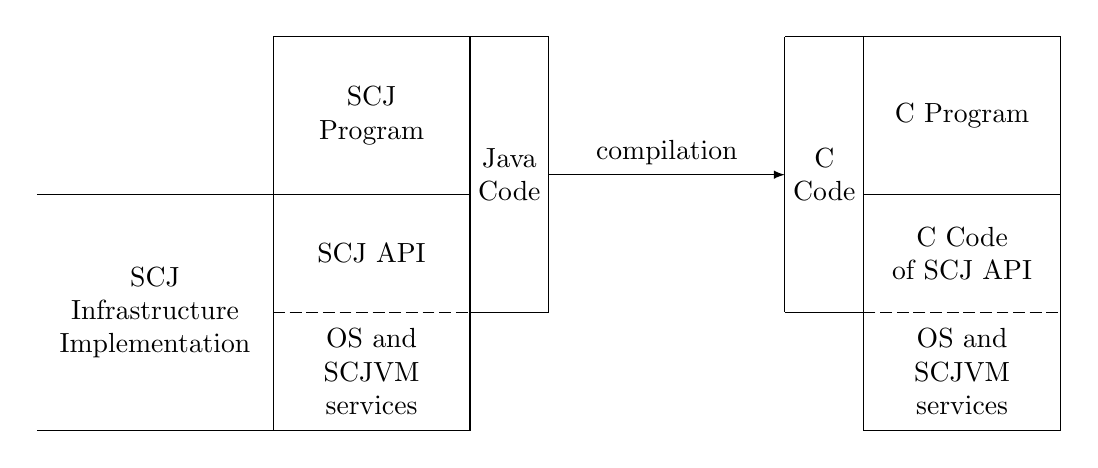
\begin{tikzpicture}
    \path (0,0) -- (0,5)
    node[pos=0.0] (bottom) {}
    node[pos=0.3] (machineBoundary) {}
    node[pos=0.6] (codeBoundary) {}
    node[pos=1.0] (top) {};

    \path (0,0) -- (10,0)
    node[pos=-0.3] (left) {}
    node[pos=0.00] (preCompilationLeft) {}
    node[pos=0.25] (preCompilationRight) {}
    node[pos=0.35] (JavaRight) {}
    node[pos=0.65] (CLeft) {}
    node[pos=0.75] (postCompilationLeft) {}
    node[pos=1.00] (postCompilationRight) {}
    node[pos=1.00] (right) {};

    \draw (bottom -| preCompilationLeft) rectangle (top -| preCompilationRight);
    \path (bottom -| preCompilationLeft) rectangle (machineBoundary -| preCompilationRight) coordinate[pos=0.5] (PreVM);
    \draw[dashed] (machineBoundary -| preCompilationLeft) rectangle (machineBoundary -| preCompilationRight);
    \path (machineBoundary -| preCompilationLeft) rectangle (codeBoundary -| preCompilationRight) coordinate[pos=0.5] (PreAPI);
    \draw (codeBoundary -| preCompilationLeft) rectangle (codeBoundary -| preCompilationRight);
    \path (codeBoundary -| preCompilationLeft) rectangle (top -| preCompilationRight) coordinate[pos=0.5] (PreCode);

    \node[align=center] at (PreVM) {OS and\\SCJVM\\services};
    \node[align=center] at (PreAPI) {SCJ API};
    \node[align=center] at (PreCode) {SCJ\\Program};

    \draw (bottom -| left) -- (bottom -| preCompilationLeft);
    \draw (codeBoundary -| left) -- (codeBoundary -| preCompilationLeft);
    \path (bottom -| left) -- (codeBoundary -| preCompilationLeft) coordinate[pos=0.5] (SCJVM);
    \node[align=center] at (SCJVM) {SCJ\\Infrastructure\\Implementation};

    \draw (top -| preCompilationRight) -- (top -| JavaRight);
    \draw (machineBoundary -| preCompilationRight) -- (machineBoundary -| JavaRight);
    \path (machineBoundary -| preCompilationRight) -- (top -| JavaRight) coordinate[pos=0.5] (JavaCode);
    \draw (machineBoundary -| JavaRight) -- (top -| JavaRight) coordinate[pos=0.5] (JavaCodeMid);
    \node[align=center] at (JavaCode) {Java\\Code};
    
    \draw (bottom -| postCompilationLeft) rectangle (top -| postCompilationRight);
    \path (bottom -| postCompilationLeft) rectangle (machineBoundary -| postCompilationRight) coordinate[pos=0.5] (PostVM);
    \draw[dashed] (machineBoundary -| postCompilationLeft) rectangle (machineBoundary -| postCompilationRight);
    \path (machineBoundary -| postCompilationLeft) rectangle (codeBoundary -| postCompilationRight) coordinate[pos=0.5] (PostAPI);
    \draw (codeBoundary -| postCompilationLeft) rectangle (codeBoundary -| postCompilationRight);
    \path (codeBoundary -| postCompilationLeft) rectangle (top -| postCompilationRight) coordinate[pos=0.5] (PostCode);

    \node[align=center] at (PostVM) {OS and\\SCJVM\\services};
    \node[align=center] at (PostAPI) {C Code\\of SCJ API};
    \node[align=center] at (PostCode) {C Program};

    \draw (top -| CLeft) -- (top -| postCompilationLeft);
    \draw (machineBoundary -| postCompilationLeft) -- (machineBoundary -| CLeft);
    \path (machineBoundary -| postCompilationLeft) -- (top -| CLeft) coordinate[pos=0.5] (CCode);
    \draw (machineBoundary -| CLeft) -- (top -| CLeft) coordinate[pos=0.5] (CCodeMid);
    \node[align=center] at (CCode) {C\\Code};
    
    \draw[-latex] (JavaCodeMid) -- node[above] {compilation} (CCodeMid);
    
  \end{tikzpicture}
  \caption{The relation of an SCJ program to the SCJ infrastructure
    in compilation}
  \label{program-infrastructure-compilation-figure}
\end{figure}

\addchange{Changed discusssion of Figure 6.2 to better explain why we
  consider the program methods but not the API methods in the code
  comparison}
\added{
After generating the code for each of our examples, we have evaluated
the examples by comparing the code generated by our prototype for each
of the program methods to that generated by icecap.
We focus on the methods of the example programs themselves, rather
than the methods of the SCJ API, which are compiled along with the
program code.
}
\deleted{
  Our main focus here is validating the compilation of the SCJ
  programs themselves, which is separate from the SCJ infrastructure
  it depends on.
  Both icecap and our strategy, however, operate on complete SCJ
  programs, including the Java code that implements the SCJ API.
}
\changed{This can be seen in}
Figure~\ref{program-infrastructure-compilation-figure}, which
\changed{shows} the structure of an SCJ program in relation to the
infrastructure and compilation.

\added{
The SCJ program depends on the SCJ infrastructure implementation,
which consists of an SCJ API implementation, possibly written in Java,
and the OS and SCJVM services, written in some native language.
Only the parts written in Java are subject to compilation, so the OS
and SCJVM services are not included in the compilation.
}
How much of the SCJ API implementation is written in Java, and hence
included in the code that undergoes compilation, depends upon the
\changed{OS and SCJVM services}.
These are generally accessed through native method calls in Java code,
but are usually implementation-defined and not visible to end-users,
as indicated by the dashed line in
Figure~\ref{program-infrastructure-compilation-figure}.

% The infrastructure in our model is accessed via special methods
% representing these native methods, but our model of the SCJ
% infrastructure is intended to model a wider part of the SCJ
% infrastructure than that which icecap implements in C.
In our model, native methods are represented by special methods, which
are called using channels, rather than bytecode invoke instructions.
Our model of the infrastructure covers the elements in the SCJ
standard. 
In icecap, however, some are implemented in Java, and some are
implemented in C. 
So, when compared to our compilation, icecap deals with more Java code
than we do.
To account for these differences when passing the examples through the
compilation strategy, we provide a small implementation of part of the
SCJ API, linking the SCJ code of the examples to the SCJVM via the
special methods in our model.

\added{
The SCJ API implementation code passed to our prototype is thus
different from the SCJ API implementation used by icecap, although the
program code is the same, since the methods of the SCJ API are the
same and it is only their implementation that differs.
}
\deleted{
This does not affect the correctness of the examples or the validity
of the comparisons, since the SCJ API is the same for both icecap and
our implementation; it is only the implementation of the API that
differs.
}
We thus focus on the program code in our evaluation of the examples.
\deleted{
After compilation, the code corresponding to the methods of the SCJ
API is still separate from the code corresponding to the methods of the SCJ
program, as indicated in
Figure~\ref{program-infrastructure-compilation-figure}, so they can be
easily distinguished.
}
Ensuring the correctness of the API implementation is a separate
issue, work on which has begun in~\cite{freitas2016}.

% In order to best compare the code generated from the examples, we have
% tried to keep the code passed to icecap and our strategy as similar as
% possible but, since much of the SCJ infrastructure relies on direct
% interaction with the SCJVM to provide features such as scheduling and
% memory management, we have provided our own library covering part of
% the SCJ API.
% Our implementation of the SCJ API is generally a quite thin layer,
% providing the required classes of SCJ and linking the SCJ code to the
% SCJVM via the special methods in our model, which represent native
% methods in the Java code.
% Much of the SCJ infrastructure is already represented in our model by
% the $Launcher$ and SCJVM services, so it is not necessary to provide
% code for it in our SCJ API implementation.
% The API we provide is the same as that for icecap, so the compilation
% results for the code of the examples themselves are similar.

\addchange{Added explanation of how code is compared, and structure of
  the discussion of the examples}
\added{
In comparing the methods of the program, we have noted the
similarities and differences between our code and the code generated
by icecap, and considered why each of the differences is present.
The code used in our comparison can be found in
Appendix~\ref{example-c-code-appendix}.

We also note that confidence in the well-formedness our code is
provided by the fact that it compiles without errors or warnings on
GCC 7.3.0, using the command \mbox{\texttt{gcc -c -Wall -pedantic}}.
The choice of warning flags for this compilation matches those used by
icecap when launching an icecap program from within Eclipse.
We note that our code can only be compiled, and not linked, as
creating a SCJVM services implementation to link to our program code
is outside the scope of this work.

In what follows, we describe each of the examples and discuss points
of our translation to C code that are particularly relevant to each
example.
While our overall comparison above focusses on the program code, we do
also make some reference in the following discussion to the SCJ API
implementation where it better illustrates some of our points.
In Section~\ref{code-comparison-subsection}, we include a general
discussion of the similarities and differences observed while
comparing the code generated by our prototype to that generated by
icecap for the program methods of each example.
}

\subsection{\texorpdfstring{\texttt{PersistentSignal}}{PersistentSignal}}
\label{persistent-signal-subsection}

Our first example is \texttt{PersistentSignal}. 
It consists of a single mission with two event handlers:~a periodic
handler, \texttt{Producer}, and an aperiodic handler, \texttt{Worker}.
These communicate through an instance of a third class,
\texttt{PersisentSignal}, after which the example is named.
The \texttt{PersisentSignal} class contains a boolean flag, with
\texttt{synchronized} methods to read, set and clear it.
\texttt{Producer} releases clear the \texttt{PersistentSignal} flag,
and then signals for the \texttt{Worker} to release.
The \texttt{Worker} sets the \texttt{PersistentSignal} flag during its
release and the \texttt{Producer} checks the flag to see if the
\texttt{Worker} has finished its release.
Both the \texttt{Producer} and \texttt{Worker} produce output to
indicate when they are released.

The main purpose of this example is to demonstrate SCJ's scheduling
behaviour.
The priority of the \texttt{Worker} is set higher than the priority of
the \texttt{Producer}, so the \texttt{Worker} always preempts the
\texttt{Producer}, leaving the flag set at the end of its release
before allowing the \texttt{Producer} to finish its release.
This means that the synchronisation applied to the methods of
\texttt{PersistentSignal} may not be necessary, but it is good
practice due to the possibility of release jitter whereby the
scheduler may switch to a thread after a small delay if, for example,
the scheduler is running on its own thread or in response to clock
interrupts.

The code generated by our prototype for this example is similar to
that generated for it by icecap.
The operations on local variables and the operand stack are
represented by operations on C variables in both the code icecap
generates and the code resulting from our strategy. 
The names of the variables differ between icecap and our
implementation, since icecap uses the local variable names from the
original SCJ code, which are included in class files for debug
purposes, but different names can be used without affecting the
correctness of the code.

The synchronisation behaviour is particularly evident in this example,
and is handled the same in both the code from icecap and the code from
our prototype.
The lock is taken just before a call to a synchronized method, and
released at the end of the synchronized method.
In our model this is represented by the $takeLock$ and $releaseLock$
channels; icecap uses a \texttt{handleMonitorEnterExit()} function to
handle both, passing a boolean flag to it to distinguish between taking
the lock and releasing the lock.
The objects locked on are the same in our code as for icecap:~the
first argument on the stack when calling the method, and the first
local variable when returning from the method.

\addchange{Removed text explaining general differences between our
  code and icecap, since it is stated later}
\deleted{
  There are some differences, most of which
  apply to all the examples discussed in this section.
  The code from icecap has extra code to throw and handle exceptions,
  which we do not consider in our model since SCJ code can be checked
  to ensure exceptions will not be thrown.
  Handling of exceptions in our strategy is a possibility for future
  work, although it is not necessary for any of our examples.
}

\deleted{
Jumps in the bytecode are translated by icecap using \texttt{goto}
statements in C.
This allows bytecode instructions to be translated more directly, but
it means the resulting code is not fully MISRA-C compliant.
In our compilation strategy, we avoid the use of \texttt{goto} by
considering the control-flow graph of each method and introducing
structures such as loops and conditionals.
This has the added advantage of making the resulting code more
readable and, since we have have certainty that this transformation
does not change the semantics of the code, it is not necessary to use
the most direct translation as icecap does.
}

\deleted{
The icecap code uses many additional variables, most of which are used
to temporarily hold values indicating whether an exception has been
thrown.
It also has a stack pointer variable, which is passed to each method
(in addition to the method's arguments) and used, in addition to the
other variables, to hold some values so that the compiled code can be
mixed with interpreted code.
As this feature is not required in our work, we do not include a stack
pointer in the code generated by our compilation strategy.
The cases where extra variables are eliminated in our strategy are
matched by icecap, such as comparing variables representing stack
slots directly in conditionals, rather than copying them into
intermediate variables, which are removed by
Rule~[\nameref{eliminate-value1-value2-conditional-rule}] in our
strategy.
}

\subsection{\texorpdfstring{\texttt{Buffer}}{Buffer}}
\label{buffer-subsection}

Our second example is \texttt{Buffer}, which, like the previous
example, consists of two event handlers:~a periodic handler,
\texttt{Producer}, and an aperiodic handler, \texttt{Consumer}.
During a release of \texttt{Producer}, it calls the
\texttt{executeInOuterArea()} method of \texttt{ManagedMemory},
passing in an anonymous \texttt{Runnable} object stored in a field
\texttt{\_switch} of \texttt{Producer}.
The \texttt{run()} method of the object in \texttt{\_switch} allocates
an instance of \texttt{Object} and stores it in a field \texttt{data}
of \texttt{Producer}.
Since it is executed via \texttt{executeInOuterArea()}, this instance
of object is allocated in the memory area outside the per-release
memory for \texttt{Producer}, which is the mission memory.
The object in \texttt{data} is then stored in a buffer and the
\texttt{Consumer} is released, which pops the object from the buffer.

The purpose of this example is to demonstrate the memory behaviour of
SCJ.
Since the object passed via the buffer is used by both event handlers,
it must be allocated in mission memory to ensure that it is available
to both event handlers.
Since objects are, by default, allocated in an event handler's
per-release memory area during its release, this allocation must be
performed via \texttt{executeInOuterArea()}.
The buffer itself must also be allocated in mission memory, but it
does not require use of \texttt{executeInOuterArea()}, since it is
allocated during mission initialisation.
Since the mission memory is not cleared during the mission, it would
eventually run out of space to allocate the objects with repeated
releases of \texttt{Producer}.
To prevent this, the \texttt{Producer} maintains a count of how many
times it has been released and does not allocate the object or store
it in the buffer if it has been released more than a set number of
times.

\addchange{Remove mention of characteristics described for
  \texttt{PersistentSignal}, since the discussion has been moved
  later}
\deleted{
The code generated from this example has many of the same
characteristics we have already described for the
\texttt{PersistentSignal} example.
In particular, the methods of the buffer are synchronized, so
synchronisations are produced in the code around calls to such
methods.
In addition, we make some further considerations related to the how
the use of the \texttt{executeInOuterArea()} method is represented in
the code.
}
\added{
We make some consideration related to the how the use of the
\texttt{executeInOuterArea()} method is represented in the code, since
it provides a good example of how method calls are translated.
}
The call to \texttt{executeInOuterArea()} itself is a simple static
method call in both the code generated by icecap and the code
generated by our strategy, since the SCJ API does not differ between
them.
Although the implementation of the method differs between the icecap
code and the code from our strategy, due to the differing SCJ
libraries used, they both contain code to change the memory area, a
call to the \texttt{run()} method of the \texttt{Runnable} object
passed into the method, and code to change the memory area back to its
previous value.

The call to the \texttt{run()} method of the \texttt{Runnable} object
is interesting as many classes in the SCJ infrastructure implement
\texttt{Runnable}, providing a large set of possible targets for the
call.
There is a large difference in the set of targets chosen for the
method call by icecap and our prototype --- the icecap code lists 10
targets, whereas our code lists 4.
The only target that appears on both lists is \texttt{Producer\$1},
the anonymous class in \texttt{Producer} that is the actual target of
the \texttt{executeInOuterArea()} call we are considering.
The other three targets in our code are all subclasses of
\texttt{AsyncEventHandler}, which is part of the superclass hierarchy
for event handlers. 

\texttt{AsyncEventHandler} is included in the list of choices for
icecap and is selected there by searching the superclasses of the
object the method is called on until one of the listed targets is
found.
In our code, we adopt a different approach, selecting using the
object's actual type but directing the call to the class in which the
method is defined.
This means that while there are three branches of the choice
corresponding to subclasses of \texttt{AsyncEventHandler}, the
contents of those branches are the same call to
\texttt{AsyncEventHandler}'s \texttt{run()} method.
This is simply a static resolution of the superclass search that
icecap conducts, for each of the possible subclasses of
\texttt{AsyncEventHandler} in the example program, so it is
equivalent.
The other targets listed in the icecap code are parts of the SCJ
infrastructure that are handled in our model by the $Launcher$ and
SCJVM services.

%TODO: say something about how targets are chosen here?

\subsection{\texorpdfstring{\texttt{Barrier}}{Barrier}}
\label{barrier-subsection}

Our third example is \texttt{Barrier}, which demonstrates a common
pattern in real-time systems, where an event only happens when
multiple event handlers have signalled their readiness.
It is based around a class named \texttt{Barrier}, which implements
this pattern.
There are three types of event handlers in this
example:~\texttt{FireHandler}, which is the type of aperiodic event
handlers that must signal their their readiness to the
\texttt{Barrier}, \texttt{LaunchHandler}, the aperiodic handler that
releases when all the \texttt{FireHandler}s have signalled their
readiness, and \texttt{Button}, a periodic handler that simulates
events releasing the \texttt{FireHandler}s.
In the example, two instances of \texttt{FireHandler} are created,
with corresponding \texttt{Button} event handlers:~one that releases
every 2 seconds, and one that releases every 9 seconds.

When a \texttt{FireHandler} releases, it checks if it has already
triggered the \texttt{Barrier}, and calls a method of the
\texttt{Barrier} to trigger it if it has not already been triggered,
passing a numerical identifier.
When the \texttt{Barrier} is triggered, it sets a boolean flag
corresponding to the passed numerical identifier, then checks if all
the boolean flags are set.
When all the boolean flags are set, the \texttt{Barrier} releases its
associated \texttt{LaunchHandler} object and resets all the boolean
flags.
The \texttt{LaunchHandler} gives output to indicate when it is
released.

This example shows a more complex scheduling behaviour than that of
the previous examples.
The \texttt{FireHandler} and \texttt{LaunchHandler} event handlers
have higher priority than the \texttt{Button} event handlers, so they
cannot be interrupted by the periodic events firing.
However, the \texttt{FireHandler} and \texttt{LaunchHandler} handlers
have the same priority, and the methods of \texttt{Barrier} are
synchronized, so the boolean flags in \texttt{Barrier} are completely
reset before the \texttt{LaunchHandler} executes.
Due to the differing periods for the \texttt{Button} handlers, the
first \texttt{FireHandler} releases four or five times before the second
\texttt{FireHandler} releases and \texttt{LaunchHandler} executes.

A particular feature of interest in the code generated for this
example stems from the fact that it has multiple aperiodic event
handler types.
This means that a release of an aperiodic handler in our code (as may
occur when the \texttt{Barrier} is triggered) is represented by a
choice between them, although both branches of the choice contain a
call to the \texttt{release()} method of
\texttt{AperiodicEventHandler}.
The corresponding icecap code simplifies this to a direct call to the
\texttt{release()} method of \texttt{AperiodicEventHandler}, omitting
the unnecessary choice.
Such a transformation could be made in our strategy, although fully
applying it involves eliminating the $getClassIDOf$ communication used
to get the class identifier used in the choice.
As explained in
Section~\ref{compilation-final-considerations-section}, this requires
operating on multiple processes and so we leave it to future work.
% This is an example of the case discussed earlier where we cannot
% eliminate the choice in our code without operating on multiple
% processes, so applying such a simplification in our strategy is left
% to future work.
Note that the fact that there are multiple instances of
\texttt{Button} and \texttt{FireHandler} makes no difference to either
the code from icecap or the code from our strategy.

\addchange{Added subsection describing the similarities and differences
  observed when comparing code}
\added{
\subsection{Code comparison}
\label{code-comparison-subsection}

We observed various similarities between our code and that generated
by icecap.
Firstly, variables are generated to store the contents of stack slots
in both, with values being pushed to the stack by assignment to these
variables, and operations performed upon them.
Local variables of a method are also represented by C variables, and
arguments of the method are passed as arguments of the C function in
both our code and icecap's code.
There are some differences in the names of variables (we name
variables using \texttt{var} and a number while icecap uses the name
of the variable from Java), and icecap distinguishes stack slots for
different types, however, the basic approach is the same.

Method calls also display similarities, particularly for non-virtual
method calls, which are simple C function calls in both our code and
icecap's code.
Virtual method calls display some differences in how the method to be
called is selected (discussed below), but the method call itself is as
in the non-virtual case.
Calls to \texttt{synchronized} methods are also compiled in the same
way, with the lock being taken on an object before the method is
called and released just before the method ends, where the operations
of taking and releasing locks are performed by calls to infrastructure
functions.

We have also observed that field accesses are the same in both our
code and in icecap.
The fields are accessed in our code by casting a variable storing the
pointer to the object, first to \texttt{uintptr\_t} to ensure it is
expanded correctly on systems where pointers are wider than 32 bits
(since a single variable is a 32-bit integer in our code), then
casting to a pointer to the struct type for the object's class, and
then accessing the field via a C field access.
The icecap code performs the access in the same way, although an
intermediate variable is used, a custom \texttt{pointer} type is used
in place of \texttt{uintptr\_t}, a few other pointer casts are applied
before the final cast to the class struct, and an optional memory
offset is allowed for.
The intermediate variable does not affect the semantics of the access,
nor do the additional pointer casts.
The \texttt{pointer} type is defined to be equivalent to the C99
\texttt{uintptr\_t} type (although it handles those compilers that may
not support C99), so that does not affect the semantics.
For the memory offset, we assume memory addresses used by the memory
manager are small enough to fit in a 32-bit JVM word.
Future work could add an offset to handle heaps outside that range if
necessary.

We also observed various differences between our code and icecap; many
of these relate to areas we have explicitly not considered in our
strategy.
In other cases, we have chosen to diverge from icecap's approach.

Firstly, there are several methods in our code that do not have
corresponding methods in the code generated by icecap.
This is due to a combination of different factors.
Some methods are not present in the code input to icecap code due to
differences in the version of the SCJ API used by our code and icecap.
Other methods are present in the code input to both our prototype and
icecap, yet have no C code generated for them in icecap.
The lack of code for these methods in icecap is due to a difference
between our prototype and icecap in how the set of methods to be
compiled is computed.
Our prototype generates C code for all methods passed to it, whereas
icecap computes which methods are required for the program, beginning
from the main method that forms the starting point of the launcher.
While this does exclude one method
(\texttt{main\_BoundedBuffer\_isFull}) that is defined in the example
code but not used, the other methods have no corresponding icecap code
due to the fact that they appear not to be called in icecap's launcher
infrastructure.
This would appear to be a deficiency in icecap's implementation of the
SCJ startup procedure, where fixed sizes are used for the immortal and
mission memory rather than obtaining them from the \texttt{Safelet}
and \texttt{Mission} provided by the program.

Another difference is that the icecap code passes a frame pointer,
\texttt{fp}, to each function and defines a stack pointer variable,
\texttt{sp}, in each function.
These are used to manage a stack, which is used in addition to the
stack slot variables.
This stack allows the compiled code to interact with interpreted code,
since the interpreted code uses this stack rather than having
predefined stack slots (which are computed during the compilation
process).
We do not require this feature in our code, since all our code is
compiled.
For the same reason, we also do not generate the code swapping stack
slot variables to and from this stack.
There are also some infrastructure methods in icecap that accept their
arguments using the stack, and a few of the generated functions in the
icecap code (such as \texttt{main\_BoundedBuffer\_init}) pop their
arguments from the stack rather than taking them as function
arguments.
This is, of course, unnecessary for our code, where we adopt the same
approach of passing arguments as C function arguments for all methods.

The icecap code also uses a different approach for returning values
from functions.
In the icecap code, return values are passed using the stack passed
into the function, with the return value popped from the stack in the
calling function.
In our code, we do not pass a stack pointer, so pointers to the stack
slot variables in which the return values are to be placed are passed
instead.
This approach used in our code is preferable to using C return values
as it scales better to \texttt{long} values, which require two
variables.
We note that icecap functions returning small values, particularly
\texttt{boolean} values in the case of our examples, instead use the
\texttt{int16} value returned from each function (normally used to
signal exceptions in the icecap code) to pass the return value.
This is a somewhat inconsistent approach to passing the return values,
but it perhaps makes best use of space for small values.

There is a lot of exception handling code in icecap that is not
present in our code, since we do not handle exceptions.
% The extra code that is present in icecap includes extra varibles to
% hold exception information, checks for null pointers before array
% accesses and method calls, checks after method calls to determine if
% an exception was thrown by the method, exception handler code at the
% end of the function, and return values communicated to indicate if an
% exception has been thrown.
As we have already seen, the return values for signalling exceptions
are also used to pass small return values of the method.
We omit the return values completely in our code, since we do not need
to signal exceptions, but our system of passing method return values
frees up the function return value for use as part of an exception
handling system in future work.

There is also a difference in how control flow constructs are
compiled.
Jumps in the bytecode are translated by icecap using \texttt{goto}
statements in C.
This allows bytecode instructions to be translated more directly, but
it means the resulting code is not fully MISRA-C compliant.
In our compilation strategy, we avoid the use of \texttt{goto} by
considering the control-flow graph of each method and introducing
structures such as loops and conditionals.
This has the added advantage of making the resulting code more
readable and, since we have have certainty that this transformation
does not change the semantics of the code, it is not necessary to use
the most direct translation as icecap does.

Differences in the code arising from the different API provided for
our code versus icecap also show themselves in the generated code.
Arrays operations in icecap are translated using C array accesses but,
since we do not have arrays, we model them as objects.
It is expected that future work that adds handling of arrays to our
compilation strategy would produce code similar to that of icecap.
There are also some places where \texttt{static} fields holding
constant values for memory sizes are additionally declared
\texttt{final} in our code, where in icecap they merely hold the same
value as a \texttt{final} field.
This means accesses to these fields appear in the icecap code, but the
values of the fields are inlined in our code.
However, from \texttt{static} field accesses in our SCJ API
implementation (such as in \texttt{devices\_Console\_read} for each of
the examples), we see that they are translated in the same way in our
code as in icecap:~by an access to a field of a global struct
containing class fields.

Finally, there is also a difference in how virtual method call targets
are chosen in our code versus that of icecap.
In icecap, the superclasses of the target object are searched to
determine which method should be executed, whereas in our code a
choice is made over the class of the target object, with the
superclasses searched at compile time.
Our approach means the work of searching for the class containing the
definition need not be performed at runtime, but results in several
conditional branches with the same body for classes that have a common
superclass.
As a future optimisation in our code, such branches could be merged
and a switch statement could be used for a more efficient choice over
classes.
The icecap code also removes the search entirely if there is only a
single possible target.
Such a transformation could be made in our strategy, although fully
applying it involves eliminating the $getClassIDOf$ communication used
to get the class identifier used in the choice.
As explained in
Section~\ref{compilation-final-considerations-section}, this requires
operating on multiple processes and so we leave it to future work.
In any case, the different approaches to selecting the target method
yield the same target at run-time.

We also noted a difference in the size of the code generated by our
prototype versus that generated by icecap.
Our prototype generates two files for each example:~a \texttt{.c} file
containing the code for each of the methods, and a \texttt{.h} file
containing struct definitions and prototypes for infrastructure
functions (the provision of which is outside the scope of this
thesis).
The files generated by icecap include many pre-defined files, that do
not result from compilation of the examples.
Namely, the files that are generated by icecap from the code of each
of the examples are a \texttt{methods.c} file, containing the code of
each method, a \texttt{methods.h} file, defining constants used to
identify each of the methods, a \texttt{classes.c} file, defining
variables containing class information, and a \texttt{classes.h} file,
defining struct types for the objects of each class.
The \texttt{methods.c} file corresponds to the \texttt{.c} file
generated by our prototype, and the \texttt{classes.h} file
corresponds to the \texttt{.h} file generated by our prototype. 
So we compare the sizes of those files.
The class information in \texttt{classes.c} and the method identifiers
in \texttt{methods.h} are included in icecap to support interpretation
of bytecode, which is not necessary in our code, so we do not include
these files in our comparison.

The sizes of the \texttt{.c} files are:~2576 lines for
\texttt{PersistentSignal}, 2748 lines for \texttt{Buffer}, and 2787
lines \texttt{Barrier}.
The sizes of the corresponding \texttt{methods.c} files generated by
icecap are~63968 lines for \texttt{PersistentSignal}, 65383 lines for
\texttt{Buffer}, and 64619 lines for \texttt{Barrier}.
The sizes of the \texttt{.h} files are:~542 lines for
\texttt{PersistentSignal}, 560 lines for \texttt{Buffer}, and 551
lines \texttt{Barrier}.
The sizes of the corresponding \texttt{classes.h} files generated by
icecap are~1164 lines for \texttt{PersistentSignal}, 1187 lines for
\texttt{Buffer}, and 1181 lines for \texttt{Barrier}.
Note that these sizes are the size of the complete files, including
blank lines and comments.

The icecap files are clearly much larger, but this includes the larger
SCJ API implementation of icecap.
Extracting the definitions of each of the program methods from the
\texttt{.c} generated by the prototype gives 362 lines for
\texttt{PersistentSignal}, 508 lines for \texttt{Buffer}, and 547
lines for \texttt{Barrier}.
Similarly, extracting the program method definitions from the
\texttt{methods.c} files generated by icecap gives 1634 lines for
\texttt{PersistentSignal}, 2041 lines for \texttt{Buffer}, and 2241
lines for \texttt{Barrier}.
The difference in size for the program methods is smaller, but the
size of the icecap method code is still more than four times the size
of the code generated by our prototype for each example.
This is, however, largely accounted for by the fact that icecap
includes extra code for exception handling and comments indicating
which line of the original Java code each line of C code corresponds
to.
For both our prototype and icecap, the C code is longer than the
original Java files, the sizes of which are: 270 lines for
\texttt{PersistentSignal}, 343 lines for \texttt{Buffer}, and 318
lines for \texttt{Barrier}.
The input to icecap also includes an additional 10-line file
containing a \texttt{main()} method that invokes icecaps launcher
infrastructure, and may be taken as part of the $Launcher$ in our
model.
The longer size for the C code over the Java code follows from the
fact that each line of Java code may be translated by multiple
bytecode instructions.

Overall, our code is similar to that of icecap; differences are
justified in that they are more suited to the particular code we are
considering.
This thus provides additional confidence in the validity of the code
generated by our strategy.
}
\section{Final Considerations}
\label{evaluation-final-considerations-section}

In this chapter, we have considered various ways in which our model
and compilation strategy can be evaluated, and their correctness
validated.
The models used as input to the strategy have been validated by using
CZT to perform syntax and type checking, and performing some proofs
using Z/EVES on the schemas defining instruction semantics.
We have seen that this ensures that the model is well-formed and
provides a means to deduce the preconditions that must be satisfied
for each bytecode instruction.
The preconditions found match those checked by JVM bytecode
verification, ensuring our semantics is correct for standard Java
bytecode.

We have also discussed the proofs of the compilation rules and the
source of the laws used used to prove those rules, seeing that the
algebraic proof style of the rules gives great certainty of the
proof's correctness by formally justifying each step in the proof.
As we mentioned, the laws we have used come from existing \Circus{}
laws taken from various sources and laws we have proved in
Isabelle/UTP.
This basis of laws known to be correct provides futher assurance of
the correctness of the proofs.

Finally, we have discussed our prototype implementation of the
compilation strategy and the assurance that may be gained from
considering some examples.
The tool shows how the individual compilation rules fit together as a
complete whole, allowing us to check how the rules act as part of the
strategy.
The examples we have considered show that the code we generate is
generally comparable to that generated by icecap.
The few differences observed between our code and icecap's code arise
from design choices that enhance the generated code.

\addchange{Added discussion of execution time and complexity of prototype}
\added{
While we have used the prototype to check form of the generated code,
it can also give us an idea of the complexity of the strategy that we
can use to judge how viable it would be were we to make a full
implementation of it.
By packaging the prototype as a \texttt{.jar} file we can execute it
from a command line and use the \texttt{time} command to measure its
execution time.
Averaging wall-clock time across 10 runs of the prototype for each of
our examples yields 2.50 seconds for \texttt{PersistentSignal}, 2.78
seconds for \texttt{Barrier} and 2.67 seconds for \texttt{Buffer}.
From the output of the prototype indicating which stages of the strategy
are executing, the bulk of this time appears to be spent in
introducing sequential composition.
More detailed tracing of the time taken shows that this is due to the
fact that the control flow graph is reconstructed after each
compilation rule is applied.
The number of reachable nodes is very high at the start of the
compilation strategy, but reduces by a large amount during sequential
composition introduction since most of the edges between nodes
represent sequential composition.
This time could be reduced by using a more sophisticated strategy to
perform local updates of the control flow graph, potentially reducing
the execution time of the prototype by up to 2 seconds.
With other optimisations, such as more efficient data structures and
pattern matching strategies, this could give reasonable execution
time, even for large programs.

It is difficult to produce similar measurements of compilation time
for icecap, since icecap is designed as an Eclipse plugin and cannot
be separated from Eclipse to allow measurment of compilation time.
However, we note that the compilation time for our examples in icecap
seems to be of the same order of magnitude as for our prototype.

Our implementation is just a prototype and so any measurments of its
running time are only approximations of the efficiency of our
compilation strategy.
It is more helpful to consider the asymptotic complexity of the
compilation strategy, to determine if it will scale well in an
optimised implementation.
Assuming an input program consists of $m$ methods containing an
average of $n$ instructions each, and that the local updates of the
control flow graph are made to take constant time, then the time
complexity of our strategy is at most $\mathcal{O}(m^3n)$.
This is because the loop on line~\ref{algorithm-method-loop} may loop
once for each of the $m$ methods if only one method is separated in
each iteration, and within the loop
Algorithm~\ref{resolve-method-calls-algorithm} checks each method call
instruction, of which there may be up to $mn$, and for each target of
the method call, of which there could be as many as there are methods,
$m$, searches its superclasses for an implementation, of which there
may be as many as ther are methods, $m$.

None of the other algorithms contributes as much as
Algorithm~\ref{resolve-method-calls-algorithm} to the time complexity,
since all the other elimination of program counter algorithms simply
iterate over each node in at most one loop. 
Even Algorithm~\ref{introduce-forward-sequence-algorithm}, which has
two nested loops, is linear in the number of instructions, since any
additional iteration of the inner loop means a sequential composition
is introduced so the nodes are merged, thus there is one fewer node
and one fewer iteration of the outer loop.
The elimination of frame stack algorithms are generally at most
$\mathcal{O}(m^2n)$, since they may transform each call of the
potential $mn$ calls to the $m$ methods.
The data refinement of objects has a separate complexity, since it is
determined by the number of classes and fields, but it is unlikely to
contribute more to complexity than the instructions, since each field
should be accessed by at least one instruction.
The overall complexity is thus $\mathcal{O}(m^3n)$, but this is an
upper bound and in most cases iteration will not be over all methods.
It may be possible to find iteration strategies to reduce this
asymptotic complexity by iterating over the methods fewer times.
This can lead to the strategy being quadratic or linear in $m$, which
seems an acceptable complexity.
}

All these considerations serve to validate the correctness of the
model and strategy, and shows that our strategy is a viable basis for
a correct-by-construction ahead-of-time SCJ-to-C compiler.


\chapter{Conclusions}
\label{conclusions-chapter}
% three sections: summary of contributions, related work, and future
% work
In this chapter we conclude by summarising the contributions of this
dissertation in Section~\ref{summary-section}.
We then discuss directions of future work in
Section~\ref{future-work-section}.

\section{Summary of Contributions}
\label{summary-section}

\addchange{Added references to previous parts of the thesis in
  Section\protect~\protect\ref{summary-section}} We have considered
the safety-critical variant of Java\added{, in
  Section~\ref{scj-section},} and the virtual machines designed to run
programs written in it\added{, in
  Section~\ref{virtual-machines-section}}.
None of the virtual machines is formally verified and\deleted{ that}
many of them precompile programs to native code.
Given the need for a formally verified virtual machine, we have
developed a framework within which an SCJVM can be verified.

Having noted that SCJ virtual machines employ compilation, we have
surveyed some of the work on compiler correctness, particularly those
related to Java compilation\added{, in
  Section~\ref{compiler-correctness-section}}.
We have established that two approaches to compiler correctness have
been used:~the commuting-diagram approach and the algebraic approach.
We have adopted the algebraic approach and chosen \Circus{}\added{, described
in Section~\ref{circus-section},} as a specification language.

To specify an SCJVM we have identified the requirements of the virtual
machine services to support SCJ programs.
We have also constructed a formal model of those requirements in the
\Circus{} specification language.
\added{These virtual machine services requirements and their formal
  model are discussed in Chapter~\ref{scjvm-services-chapter}.}

Contact with one of the authors of the SCJ specification has allowed
us to obtain clarifications where the specification was unclear.
The development of the formal model has helped in the identification
of the areas that require clarification.
It may be noted that the interface we have defined is not the only one
that can support SCJ, but its overall functionality must be present in
all SCJ virtual machines in some way.
The SCJ specification has been changed to reflect\deleted{ of} many of
these clarifications.
In particular, the current thread during an interrupt, the backing
store space required during mission setup, and the initialisation of
the \texttt{Safelet} have all been clarified as a result of our
contact with the authors of the SCJ specification.

We have also created a formal model of the core execution environment
that executes SCJ programs in an SCJVM.
This model has been created by identifying a minimal subset of Java
bytecode and defining its semantics, and then constructing a \Circus{}
model of an interpreter for that subset with the necessary
infrastructure around it.
\added{We have discussed the core execution environment model in
  Chapter~\ref{cee-chapter}.}

Finally, we have specified a strategy for compiling SCJ bytecode to
C\added{, presented in Chapter~\ref{strategy-chapter}}.
This is a strategy to apply individual compilation rules, which are
stated as algebraic laws, to transform our model of an SCJVM
interpreter, loaded with an SCJ bytecode program, to a \Circus{}
representation of the equivalent C code.
Since the compilation rules are stated formally as \Circus{}
refinement laws, we can, and have, written proofs of them.
\added{We have discussed these proofs in
  Section~\ref{proofs-of-laws-section}.}
This allows us to be sure of their correctness, so that our
compilation strategy preserves the semantics of the original SCJ
bytecode.
In this way, we have created a strategy for correct compilation from
SCJ bytecode to C.

Our work is done in the context of a wider effort to facilitate fully
verified SCJ programs.
There has already been work on generating correct SCJ programs from
\Circus{} specifications~\cite{cavalcanti2011, cavalcanti2013} and
formalisation of the SCJ memory model~\cite{cavalcanti2011a}.
These works allow for verification of SCJ programs, with our work
covering the next stage in ensuring those programs can be run
correctly.

Since our work addresses the execution of Java bytecode, it must still
be ensured that SCJ programs can be compiled to bytecode correctly.
Since SCJ does not make any syntactic changes to Java and the
semantic changes can be dealt with at the level of Java bytecode, a
standard Java compiler suffices for SCJ.
As discussed earlier, there has been plenty of work on correct
compilation of Java programs~\cite{klein2006, strecker2002,
  lochbihler2010, duran2005, stark2001} so it can be seen that there
is already sufficient work to permit correct compilation to Java
bytecode.
This then leaves us with correct SCJ programs in Java bytecode and the
focus of our work is on the next stage of running those programs.

Finally, as we are adopting the approach of compilation to C, it must
also be ensured that the C code can be compiled correctly.
We note that there has been much work on verified C
compilation~\cite{leroy2009a, leroy2009b, leroy2012, leinenbach2005,
  blazy2006} and, in particular, that the CompCert project provides a
functioning formally verified C compiler that can be used.

\addchange{Changed concluding sentence of
  Section\protect~\protect\ref{summary-section} to be more balanced}
\added{
So, our work provides the basis for the implementation of a verified
compiler, the development of which would provide the final piece
required for complete verification of SCJ programs down to executable
code.
}
\deleted{
So our proposed work is the final piece needed for complete
verification of SCJ programs down to executable code.
}

\section{Future Work}
\label{future-work-section}

There are various possibilities for future work arising from our work.
Firstly, our work may be further validated by consideration of a wider
range of examples.
This may involve further extension of the model and compilation
strategy to consider instructions and features not covered by our
work.
These extensions would not involve significant changes to the
strategy, since most of the instructions not included in our subset
are similar to those in our subset.

A further direction for future work to validate the strategy would be
to mechanise the compilation rules and their proofs using an automated
theorem prover, such as Isabelle/UTP.
This would confirm the correctness of the rules and allow for easier
reasoning about the strategy as whole.
Code generation from such a mechanisation could also be used to
produce an implementation of the strategy.

\addchange{Added paragraph on how our work may be applied to future
  work on the algebraic approach}
\added{
Our strategy also shows how the algebraic approach developed
in~\cite{sampaio1993} may be adapted to compile from low-level
languages to higher-level languages.
Future work could build upon this to develop compilation strategies
for other low-level languages in a similar way, contributing to wider
work on the algebraic approach to compilation.
}

Other possible directions for future work include the full
verification of an SCJ virtual machine using our framework or even the
creation of a correct-by-construction virtual machine from our
specification.
The option of deriving a correct virtual machine from our
specification may be more desirable than verifying an existing one.
This is because virtual machines can often be complex and therefore
difficult to verify in a structured way.
Moreover, while the effort of proving a virtual machine correct may
uncover bugs, it may be a challenge to fix them.
Also, the design of an existing virtual machine may not exactly meet
the structure of our specification, requiring restructuring to allow
the proof effort to begin.
The work verifying the icecap scheduler in~\cite{freitas2016} shows
this, since the tight coupling between components in icecap made
modelling and verification challenging.

On the other hand, the fact that \Circus{} allows for refinement means
that a correct virtual machine can be constructed from our model in a
stepwise and modular fashion, being shown to be correct at each stage
of the process.
Facilitating such work is the ultimate aim of our work, in order to
provide for the correct running of SCJ programs.



\appendix

%TC:macro \IfFullModel [text]
%TC:macro \IfNotFullModel [ignore]
\FullModeltrue
\chapter{Compilation Rules}
\label{compilation-rules-appendix}

\section{Elimination of Program Counter}

\subsection{Expand Bytecode}

\PCExpansionRule*

\HandleInstructionRefinementRule*

\subsection{Introduce Sequential Composition}

\SequenceIntroductionRule*

\subsection{Introduce Loops and Conditionals}

\IfConditionalIntroductionRule*

\begin{restatable}[\texttt{if}-\texttt{else}-conditional-intro]{crule}{IfElseConditionalIntroductionRule}
  \label{if-else-introduction-rule}
  \setlength{\zedindent}{0.25cm}
  % \setlength{\abovedisplayskip}{0.1cm}
  % \setlength{\belowdisplayskip}{0.1cm}
  Given $i : ProgramAddress$, if $i \neq j$, $i \neq k$, and 
  \begin{circus}
    \{frameStack \neq \emptyset\} \circseq A \\
    {} = {} \\
    \{frameStack \neq \emptyset\} \circseq A \circseq \{frameStack \neq \emptyset\}
  \end{circus}
  then
  \begin{circus}
    \begin{array}{l}
      \circmu X \circspot \\
      \t1 \circif frameStack = \emptyset \circthen \Skip \\
      \t1 {} \circelse frameStack \neq \emptyset \circthen {} \\
      \t2 \circif \cdots \\
      \t2 {} \circelse pc = i \circthen A \circseq \\
      \t3 pc := \IF b \THEN j \ELSE k \\
      \t2 {} \cdots {} \\
      \t2 {} \circelse pc = j \circthen B \circseq pc := x \\
      \t2 {} \cdots {} \\
      \t2 {} \circelse pc = k \circthen C \circseq pc := x \\
      \t2 {} \cdots {} \\
      \t2 \circfi \circseq Poll \circseq X \\
      \t1 \circfi
    \end{array}
    \circrefines_A
    \begin{array}{l}
      \circmu X \circspot \\
      \t1 \circif frameStack = \emptyset \circthen \Skip \\
      \t1 {} \circelse frameStack \neq \emptyset \circthen {} \\
      \t2 \circif \cdots \\
      \t2 {} \circelse pc = i \circthen A \circseq \\
      \t3 \circif b \circthen pc := j \circseq Poll \circseq B \\
      \t3 {} \circelse \lnot b \circthen pc := k \circseq Poll \circseq C \\
      \t3 \circfi \circseq pc := x \\
      \t2 {} \cdots {} \\
      \t2 {} \circelse pc = j \circthen B \circseq pc := x \\
      \t2 {} \cdots {} \\
      \t2 {} \circelse pc = k \circthen C \circseq pc := x \\
      \t2 {} \cdots {} \\
      \t2 \circfi \circseq Poll \circseq X \\
      \t1 \circfi 
    \end{array}
  \end{circus}
\end{restatable}

\begin{restatable}[conditional-intro]{crule}{ConditionalIntroductionRule}
  \label{conditional-introduction-rule}
  \setlength{\zedindent}{0.25cm}
  % \setlength{\abovedisplayskip}{0.1cm}
  % \setlength{\belowdisplayskip}{0.1cm}
  Given $i : ProgramAddress$, if $i \neq j$, $i \neq k$, and
  \begin{circus}
    \{frameStack \neq \emptyset\} \circseq A \\
    {} = {} \\
    \{frameStack \neq \emptyset\} \circseq A \circseq \{frameStack \neq \emptyset\}
  \end{circus}
  then
  \begin{circus}
    \begin{array}{l}
      \circmu X \circspot \\
      \t1 \circif frameStack = \emptyset \circthen \Skip \\
      \t1 {} \circelse frameStack \neq \emptyset \circthen {} \\
      \t2 \circif \cdots \\
      \t2 {} \circelse pc = i \circthen A \circseq \\
      \t3 pc := \IF b \THEN j \ELSE k \\
      \t2 {} \cdots {} \\
      \t2 {} \circelse pc = j \circthen B \\
      \t2 {} \cdots {} \\
      \t2 {} \circelse pc = k \circthen C \\
      \t2 {} \cdots {} \\
      \t2 \circfi \circseq Poll \circseq X \\
      \t1 \circfi
    \end{array}
    \circrefines_A
    \begin{array}{l}
      \circmu X \circspot \\
      \t1 \circif frameStack = \emptyset \circthen \Skip \\
      \t1 {} \circelse frameStack \neq \emptyset \circthen {} \\
      \t2 \circif \cdots \\
      \t2 {} \circelse pc = i \circthen A \circseq \\
      \t3 \circif b \circthen pc := j \circseq Poll \circseq B \\
      \t3 {} \circelse \lnot b \circthen pc := k \circseq Poll \circseq C \\
      \t3 \circfi \\
      \t2 {} \cdots {} \\
      \t2 {} \circelse pc = j \circthen B \\
      \t2 {} \cdots {} \\
      \t2 {} \circelse pc = k \circthen C \\
      \t2 {} \cdots {} \\
      \t2 \circfi \circseq Poll \circseq X \\
      \t1 \circfi 
    \end{array}
  \end{circus}
\end{restatable}

\WhileLoopIntroductionRuleA*

\begin{crule}[\texttt{while}-loop-intro2]
  \label{while-introduction-rule2}
  \setlength{\zedindent}{0.2cm}
  \setlength{\zedtab}{0.9\zedtab}
  Given $i : ProgramAddress$, if $i \neq j$,
  \begin{circus}
    \{frameStack \neq \emptyset\} \circseq A \\
    {} = {} \\
    \{frameStack \neq \emptyset\} \circseq A \circseq \{frameStack \neq \emptyset\}
  \end{circus}
  then
  \begin{circus}
    \begin{array}{l}
      \circmu X \circspot \\
      \t1 \circif frameStack = \emptyset \circthen \Skip \\
      \t1 {} \circelse frameStack \neq \emptyset \circthen {} \\
      \t2 \circif \cdots \\
      \t2 {} \circelse pc = i \circthen A \circseq \\
      \t3 pc := \IF b \THEN j \ELSE k \\
      \t2 \cdots \\
      \t2 {} \circelse pc = j \circthen B \circseq pc := i \\
      \t2 \cdots \\
      \t2 {} \circelse pc = k \circthen C \\
      \t2 \cdots \\
      \t2 \circfi \circseq Poll \circseq X \\
      \t1 \circfi 
    \end{array}
    \circrefines_A
    \begin{array}{l}
      \circmu X \circspot \\
      \t1 \circif frameStack = \emptyset \circthen \Skip \\
      \t1 {} \circelse frameStack \neq \emptyset \circthen {} \\
      \t2 \circif \cdots \\
      \t2 {} \circelse pc = i \circthen (\circmu Y \circspot A \circseq \\
      \t3 \circif b \circthen \\
      \t4 pc := j \circseq Poll \circseq B \circseq pc := i \circseq Poll \circseq Y \\
      \t3 {} \circelse \lnot b \circthen C \\
      \t3 \circfi) \circseq pc := k \\
      \t2 \cdots \\
      \t2 {} \circelse pc = j \circthen B \circseq pc := i \\
      \t2 \cdots \\
      \t2 {} \circelse pc = k \circthen C \\
      \t2 \cdots \\
      \t2 \circfi \circseq Poll \circseq X \\
      \t1 \circfi 
    \end{array}
  \end{circus}
\end{crule}

\begin{restatable}[\texttt{do}-\texttt{while}-loop-intro]{crule}{DoWhileLoopIntroductionRule}
  \label{do-while-introduction-rule}
  \def\zedindent{0.25cm}
  Given $i : ProgramAddress$, if $i \neq j$,
  \begin{circus}
    \{frameStack \neq \emptyset\} \circseq A \\
    {} = {} \\
    \{frameStack \neq \emptyset\} \circseq A \circseq \{frameStack \neq \emptyset\}
  \end{circus}
  then
  \begin{circus}
    \begin{array}{l}
      \circmu X \circspot \\
      \t1 \circif frameStack = \emptyset \circthen \Skip \\
      \t1 {} \circelse frameStack \neq \emptyset \circthen {} \\
      \t2 \circif \cdots \\
      \t2 {} \circelse pc = i \circthen A \circseq \\
      \t3 pc := \IF b \THEN i \ELSE j \\
      \t2 \cdots \\
      \t2 {} \circelse pc = j \circthen B \\
      \t2 \cdots \\
      \t2 \circfi \circseq Poll \circseq X \\
      \t1 \circfi 
    \end{array}
    \circrefines_A
    \begin{array}{l}
      \circmu X \circspot \\
      \t1 \circif frameStack = \emptyset \circthen \Skip \\
      \t1 {} \circelse frameStack \neq \emptyset \circthen {} \\
      \t2 \circif \cdots \\
      \t2 {} \circelse pc = i \circthen (\circmu Y \circspot A \\
      \t3 \circif b \circthen pc := i \circseq Poll \circseq Y \\
      \t3 {} \circelse \lnot b \circthen \Skip \\
      \t3 \circfi) \circseq pc := j \\
      \t2 \cdots \\
      \t2 \circfi \circseq Poll \circseq X \\
      \t1 \circfi 
    \end{array}
  \end{circus}
\end{restatable}

\begin{restatable}[infinite-loop-intro]{crule}{InfiniteLoopIntroductionRule}
  \label{infinite-loop-introduction-rule}
  Given $i : ProgramAddress$, if
  \begin{circus}
    \{frameStack \neq \emptyset\} \circseq A \\
    {} = {} \\
    \{frameStack \neq \emptyset\} \circseq A \circseq \{frameStack \neq \emptyset\}
  \end{circus}
  then
  \def\zedindent{0.25cm}
  \begin{circus}
    \begin{array}{l}
      \circmu X \circspot \\
      \t1 \circif frameStack = \emptyset \circthen \Skip \\
      \t1 {} \circelse frameStack \neq \emptyset \circthen {} \\
      \t2 \circif \cdots \\
      \t2 {} \circelse pc = i \circthen {} \\
      \t3 A \circseq pc := i \\
      \t2 {} \cdots {} \\
      \t2 \circfi \circseq Poll \circseq X \\
      \t1 \circfi
    \end{array}
    \circrefines_A
    \begin{array}{l}
      \circmu X \circspot \\
      \t1 \circif frameStack = \emptyset \circthen \Skip \\
      \t1 {} \circelse frameStack \neq \emptyset \circthen {} \\
      \t2 \circif \cdots \\
      \t2 {} \circelse pc = i \circthen {} \\
      \t3 \circmu Y \circspot A \circseq pc := i \circseq Poll \circseq Y \\
      \t2 {} \cdots {} \\
      \t2 \circfi \circseq Poll \circseq X \\
      \t1 \circfi
    \end{array}
  \end{circus}
\end{restatable}

\subsection{Resolve Method Calls}

\IntroduceClassInformationRule*

\begin{restatable}[refine-invokespecial]{crule}{RefineInvokespecialRule}
  \label{refine-invokespecial-rule}
  \setlength{\zedindent}{0.25cm}
  \begin{circus}
    \begin{array}{l}
      \{ pc = i \} \circseq HandleInvokespecialEPC(cpi)
    \end{array}
    \circrefines_A
    \begin{array}{l}
      \{ pc = i \} \circseq \circvar poppedArgs : \seq Word \circspot \\
      \t1 \lschexpract \exists argsToPop? == methodArguments~m + 1 @ \\
      \t2 InterpreterStackFrameInvoke \rschexpract \circseq \\
      \t1 Invoke(c, m, poppedArgs, \false)
    \end{array}
  \end{circus}
  where $m : MethodID$ and $c : ClassID$ are such that
  \begin{displaymath}
    \exists c_0 : Class; m_0 : MethodID | c_0 \in \ran cs \land m_0 \in \dom c_0.methodEntry @ \\
    \t1 cpi \in methodRefIndices~c_0 \land \\
    \t1 c_0.constantPool~cpi = MethodRef~(c,m) \land \\
    \t1 i \in c_0.methodEntry~m_0 \upto c_0.methodEnd~m_0.
  \end{displaymath}
\end{restatable}

\RefineInvokestaticRule*

\begin{restatable}[refine-invokevirtual-single]{crule}{RefineInvokeVirtualSingleRule}
  \label{refine-invokevirtual-single-rule}
  \setlength{\zedindent}{0.25cm}
  \begin{circus}
    \begin{array}{l}
      \{ pc = i \} \circseq HandleInvokevirtualEPC(cpi)
    \end{array}
    \circrefines_A
    \begin{array}{l}
      \{ pc = i \} \circseq \circvar poppedArgs : \seq Word \circspot \\
      \t1 \lschexpract \exists argsToPop? == methodArguments~m @ \\
      \t2 InterpreterStackFrameInvoke \rschexpract \circseq \\
      \t1 getClassIDOf!(head~poppedArgs)?cid \\
      \t1 {} \then Invoke(c, m, poppedArgs, \false)
    \end{array}
  \end{circus}
  where $m : MethodID$ and $c : ClassID$ are such that
  \begin{displaymath}
    \exists c_0 : Class; m_0 : MethodID | c_0 \in \ran cs \land m_0 \in \dom c_0.methodEntry @ \\
    \t1 cpi \in methodRefIndices~c_0 \land \\
    \t1 c_0.constantPool~cpi = MethodRef~(c,m) \land \\
    \t1 i \in c_0.methodEntry~m_0 \upto c_0.methodEnd~m_0,
  \end{displaymath}
  and provided $\exists_1 c_1 : ClassID @ (c_1,c) \in subclassRel~cs$.
\end{restatable}

\ResolveSpecialMethodRule*

\begin{restatable}[resolve-special-method-virtual]{crule}{ResolveSpecialMethodVirtualRule}
  \label{resolve-special-method-virtual-rule}
  If $c$, $m$ and $static$ match one of the rows of
  Table~\ref{special-method-action-table}, then
  \setlength{\zedindent}{0.25cm} \setlength{\zedtab}{0.5cm}
  \begin{circus}
    \begin{array}{l}
      \{ pc = i \} \circseq \circvar poppedArgs : \seq Word \circspot \\
      \lschexpract \exists argsToPop? == e @ \\
      \t1 InterpreterStackFrameInvoke \rschexpract \circseq \\
      getClassIDOf!(head~poppedArgs)?cid \\
      {} \then Invoke(c, m, poppedArgs, static)
    \end{array}
    \circrefines_A
    \begin{array}{l}
      \circvar poppedArgs : \seq Word \circspot \\
      \lschexpract \exists argsToPop? == e @ \\
      \t1 InterpreterStackFrameInvoke \rschexpract \circseq \\
      getClassIDOf!(head~poppedArgs)?cid \\
      {} \then specialMethodAction(c, m, static) \circseq \\
      pc := i + 1
    \end{array}
  \end{circus}
  where $specialMethodAction$ is the syntactic function defined by
  Table~\ref{special-method-action-table}.
\end{restatable}

\ResolveNormalMethodRule*

\begin{restatable}[resolve-normal-method-virtual]{crule}{ResolveNormalMethodVirtualRule}
  \label{resolve-normal-method-virtual-rule}
  Given $i : ProgramAddress$, if
  \begin{circus}
    \{frameStack \neq \emptyset\} \circseq A \\
    {} = {} \\
    \{frameStack \neq \emptyset\} \circseq A \circseq \{frameStack \neq \emptyset\},
  \end{circus}
  and there exists $classInfo : Class$ in $\ran cs$ such that,
  \begin{circus}
    \{ methodID = m \land classID = c \} \circseq \lschexpract ResolveMethod \rschexpract \\
    {} = {} \\
    \{ methodID = m \land classID = c \} \circseq \lschexpract ResolveMethod \rschexpract \circseq \\
    \t1 \{ class = classInfo \land classInfo.methodEntry~m = k \},
  \end{circus}
  and, for any $x : ProgramAdress$,
  \begin{circus}
    \{ (last~(front~frameStack)).storedPC = x \} \circseq M \\
    {} = {} \\
    \{ (last~(front~frameStack)).storedPC = x \} \circseq M \circseq \{ pc = x \},
  \end{circus}
  and $m$ and $c$ do not match any of the conditions in
  Table~\ref{special-method-action-table} then,
  \setlength{\zedindent}{0cm}
  \setlength{\zedtab}{0.45cm}
  \begin{circus}
    \begin{array}{l}
      \circmu X \circspot \\
      \t1 \circif frameStack = \emptyset \circthen \Skip \\
      \t1 {} \circelse frameStack \neq \emptyset \circthen {} \\
      \t2 \circif \cdots \\
      \t2 {} \circelse pc = i \circthen A \circseq \{ pc = j \} \circseq \\
      \t3 \circvar poppedArgs : \seq Word \circspot \\
      \t3 \lschexpract \exists argsToPop? == e @ \\
      \t4 InterpreterStackFrameInvoke \rschexpract \circseq \\
      \t3 getClassIDOf!(head~poppedArgs)?cid \\
      \t3 {} \then Invoke(c, m, poppedArgs, \false) \\
      \t2 {} \circelse pc = k \circthen M \\
      \t2 \cdots \\
      \t2 \circfi \circseq Poll \circseq X \\
      \t1 \circfi 
    \end{array}
    \circrefines_A
    \begin{array}{l}
      \circmu X \circspot \\
      \t1 \circif frameStack = \emptyset \circthen \Skip \\
      \t1 {} \circelse frameStack \neq \emptyset \circthen {} \\
      \t2 \circif \cdots \\
      \t2 {} \circelse pc = i \circthen A \circseq \\
      \t3 (\circvar poppedArgs : \seq Word \circspot \\
      \t3 \lschexpract \exists argsToPop? == e @ \\
      \t4 InterpreterStackFrameInvoke \rschexpract \circseq \\
      \t3 getClassIDOf!(head~poppedArgs)?cid \\
      \t3 {} \then \lschexpract InterpreterNewStackFrame[ \\
      \t4 classInfo/class?, \\
      \t4 m/methodID?, \\
      \t4 poppedArgs/methodArgs?] \rschexpract)) \circseq \\
      \t3 Poll \circseq M \circseq pc := j + 1 \\
      \t2 {} \circelse pc = k \circthen M \\
      \t2 \cdots \\
      \t2 \circfi \circseq Poll \circseq X \\
      \t1 \circfi 
    \end{array}
  \end{circus}
\end{restatable}

\RefineInvokeVirtualMultiRule*

\begin{restatable}[resolve-special-method-branch]{crule}{ResolveSpecialMethodBranchRule}
  \label{resolve-special-method-branch-rule}
  Given $c_\ell : ClassID$, if $c = c_\ell$, $m$ and $static = \false$
  match one of the rows of Table~\ref{special-method-action-table},
  then
  \setlength{\zedindent}{0.25cm}
  \setlength{\zedtab}{0.5cm}
  \begin{circus}
    \begin{array}{l}
      \circvar poppedArgs : \seq Word \circspot \\
      \lschexpract \exists argsToPop? == e @ \\
      \t1 InterpreterStackFrameInvoke \rschexpract \circseq \\
      \circif cid = c_1 \circthen A_1 \\
      {} \cdots {} \\
      {} \circelse cid = c_\ell \circthen {} \\
      \t1 \{ (last~frameStack).storedPC = j + 1 \} \circseq \\
      \t1 Invoke(c_\ell, m, poppedArgs, \false) \\
      {} \cdots {} \\
      {} \circelse cid = c_n \circthen A_n \\
      \circfi
    \end{array}
    \circrefines_A
    \begin{array}{l}
      \{ pc = i \} \circseq \circvar poppedArgs : \seq Word \circspot \\
      \lschexpract \exists argsToPop? == e @ \\
      InterpreterStackFrameInvoke \rschexpract \circseq \\
      \circif cid = c_1 \circthen A_1 \\
      {} \cdots {} \\
      {} \circelse cid = c_\ell \circthen {} \\
      \t1 specialMethodAction(c_\ell, m, \false) \circseq pc := i + 1 \\
      {} \cdots {} \\
      {} \circelse cid = c_n \circthen A_n \\
      \circfi
    \end{array} 
  \end{circus}
  where $specialMethodAction$ is the syntactic function defined by
  Table~\ref{special-method-action-table}.
\end{restatable}

\begin{restatable}[resolve-normal-method-branch]{crule}{ResolveNormalMethodBranchRule}
  \label{resolve-normal-method-branch-rule}
  \setlength{\zedtab}{0.4cm}
  Given $i : ProgramAddress$, if
  \begin{circus}
    \{frameStack \neq \emptyset\} \circseq A \\
    {} = {} \\
    \{frameStack \neq \emptyset\} \circseq A \circseq \{frameStack \neq \emptyset\},
  \end{circus}
  and there exists $classInfo : Class$ in $\ran cs$ such that,
  \begin{circus}
    \{ methodID = m \land classID = c \} \circseq \lschexpract ResolveMethod \rschexpract \\
    {} = {} \\
    \{ methodID = m \land classID = c \} \circseq \lschexpract ResolveMethod \rschexpract \circseq \\
    \t1 \{ class = classInfo \land classInfo.methodEntry~m = k \},
  \end{circus}
  and, for any $x : ProgramAddress$,
  \begin{circus}
    \{ (last~(front~frameStack)).storedPC = x \} \circseq M \\
    {} = {} \\
    \{ (last~(front~frameStack)).storedPC = x \} \circseq M \circseq \{ pc = x \},
  \end{circus}
  and $m$ and $c$ do not match any of the conditions in
  Table~\ref{special-method-action-table} then,
  \setlength{\zedindent}{0.25cm}
  \begin{circus}
    \begin{array}{l}
      \circmu X \circspot \\
      \t1 \circif frameStack = \emptyset \circthen \Skip \\
      \t1 {} \circelse frameStack \neq \emptyset \circthen {} \\
      \t2 \circif \cdots \\
      \t2 {} \circelse pc = i \circthen A \circseq \\
      \t3 \circvar poppedArgs : \seq Word \circspot \\
      \t3 \lschexpract \exists argsToPop? == e @ \\
      \t4 InterpreterStackFrameInvoke \rschexpract \circseq \\
      \t3 \circif cid = c_1 \circthen A_1 \\
      \t3 {} \cdots {} \\
      \t3 {} \circelse cid = c_\ell \circthen {} \\
      \t4 \{ (last~frameStack).storedPC = j + 1 \} \circseq \\
      \t4 Invoke(c_\ell, m, poppedArgs, \false) \\
      \t3 {} \cdots {} \\
      \t3 {} \circelse cid = c_n \circthen A_n \\
      \t3 \circfi \\
      \t2 {} \circelse pc = k \circthen M \\
      \t2 \cdots \\
      \t2 \circfi \circseq Poll \circseq X \\
      \t1 \circfi 
    \end{array}
    \circrefines_A
    \begin{array}{l}
      \circmu X \circspot \\
      \t1 \circif frameStack = \emptyset \circthen \Skip \\
      \t1 {} \circelse frameStack \neq \emptyset \circthen {} \\
      \t2 \circif \cdots \\
      \t2 {} \circelse pc = i \circthen A \circseq \{ pc = j \} \circseq  \\
      \t3 \circvar poppedArgs : \seq Word \circspot \\
      \t3 \lschexpract \exists argsToPop? == e @ \\
      \t4 InterpreterStackFrameInvoke \rschexpract \circseq \\
      \t3 \circif cid = c_1 \circthen A_1 \\
      \t3 {} \cdots {} \\
      \t3 {} \circelse cid = c_\ell \circthen {} \\
      \t4 \lschexpract InterpreterNewStackFrame[ \\
      \t5 classInfo/class?,
      \t5 m/methodID?, \\
      \t5 poppedArgs/methodArgs?] \rschexpract) \circseq \\
      \t4 Poll \circseq M \circseq pc := j + 1 \\
      \t3 {} \cdots {} \\
      \t3 {} \circelse cid = c_n \circthen A_n \\
      \t3 \circfi \\
      \t2 {} \circelse pc = k \circthen M \\
      \t2 \cdots \\
      \t2 \circfi \circseq Poll \circseq X \\
      \t1 \circfi 
    \end{array}
  \end{circus}
\end{restatable}

\subsection{Refine Main Actions}

\RunningRefinementRule*


\chapter{C Code of Examples}
\label{example-c-code-appendix}

% undo some CZT meddling with the hash symbol
\renewcommand\#{\char"0023}

\titleformat{\section}{\needspace{10\baselineskip}\color{headcol}\large\rmfamily\bfseries}{\thesection}{1em}{#1}[]
\titleformat{\subsection}{\needspace{7\baselineskip}\color{headcol}\large\rmfamily\bfseries}{\thesubsection}{1em}{#1}[]
\titleformat{\subsubsection}{\needspace{5\baselineskip}\normalsize\rmfamily\bfseries}{\thesubsubsection}{1em}{#1}[]
\titleformat{\paragraph}{\needspace{4\baselineskip}\normalsize\rmfamily\bfseries}{\theparagraph}{1em}{#1}[]

\lstset{basicstyle=\ttfamily\footnotesize,language=C,
  numbers=left, numberstyle=\tiny, stepnumber=1, numbersep=2pt,
  escapeinside={(*@}{@*)}, linewidth=\linewidth, breaklines=true,
  tabsize=2, framexleftmargin=0.3cm, xleftmargin=0.3cm,
  postbreak=\mbox{$\!\hookrightarrow$}, breakindent=2pt}

\addchange{Added Appendix B}
This appendix contains the C code for the examples considered in
Chapter~\ref{evaluation-chapter}.
We provide the code for each example in a separate
section:~\texttt{PersistentSignal} in
Section~\ref{PersistentSignal-code-section}, \texttt{Buffer} in
Section~\ref{Buffer-code-section}, and \texttt{Barrier} in
Section~\ref{Barrier-code-section}.

For each example, we first provide the Java code used as input to our
prototype (Sections~\ref{PersistentSignal-java-code-subsection},
\ref{Buffer-java-code-subsection}
and~\ref{Barrier-java-code-subsection}).
The code input to icecap is similar, but with the addition of a file
containing a main method that invokes icecap's launcher code, passing
the safelet for the program.
Java arrays are also used in the code input to icecap, rather than the
array classes used in our code.

After the Java code for each example, we present the code generated by
our prototype for each of the program methods of the examples
(Sections~\ref{PersistentSignal-code-comparison-subsection},
\ref{Buffer-code-our-subsection}
and~\ref{Barrier-code-our-subsection}).
For the first example we also present the corresponding icecap code
for each method.
Since the icecap code is quite long and the corresponding code for
each of the constructs in our prototype code is similar, we omit the
icecap code for the other two examples here.
It can be found among the online resources that accompany this thesis
(see Section~\ref{document-structure-section} for link).

Due to the length of some of the identifiers in the code, we have
shortened the identifiers by omitting type signatures in method
and field identifiers, since there are no places in the code where
that would cause ambiguity.
This brings the identifiers closer to those used in the corresponding
icecap code.
Also, since some of the lines of code are particularly long, 
they are broken across multiple lines in our presentation.
Lines that are the continuation of a line of code in the original file
are marked with a hooked arrow (\mbox{$\hookrightarrow$}) at the start
and are not given a separate line number.

\begin{landscape}
\begin{multicols}{2}

% \Needspace{3\baselineskip}
\section{\texorpdfstring{\texttt{PersistentSignal}}{PersistentSignal}}
% \nobreak
\label{PersistentSignal-code-section}

% \Needspace{3\baselineskip}
\subsection{Java Code}
% \nobreak
\label{PersistentSignal-java-code-subsection}

% \Needspace{3\baselineskip}
\subsubsection{\texttt{MainMission.java}}
% \nobreak
\lstinputlisting{../../PhD-Workspace/ModelPersistentSignal/src/main/MainMission.java}

% \Needspace{3\baselineskip}
\subsubsection{\texttt{MainSequence.java}}
% \nobreak
\lstinputlisting{../../PhD-Workspace/ModelPersistentSignal/src/main/MainSequence.java}

% \Needspace{3\baselineskip}
\subsubsection{\texttt{MySafelet.java}}
% \nobreak
\lstinputlisting{../../PhD-Workspace/ModelPersistentSignal/src/main/MySafelet.java}

% \Needspace{3\baselineskip}
\subsubsection{\texttt{PersistentSignal.java}}
% \nobreak
\lstinputlisting{../../PhD-Workspace/ModelPersistentSignal/src/main/PersistentSignal.java}

% \Needspace{3\baselineskip}
\subsubsection{\texttt{Producer.java}}
% \nobreak
\lstinputlisting{../../PhD-Workspace/ModelPersistentSignal/src/main/Producer.java}

% \Needspace{3\baselineskip}
\subsubsection{\texttt{Worker.java}}
% \nobreak
\lstinputlisting{../../PhD-Workspace/ModelPersistentSignal/src/main/Worker.java}

% \Needspace{3\baselineskip}
\subsection{Comparison of program code}
\label{PersistentSignal-code-comparison-subsection}
% \nobreak

% \Needspace{3\baselineskip}
\subsubsection{\texttt{main\_MySafelet\_globalBackingStoreSize}}
% \nobreak

% \Needspace{3\baselineskip}
\paragraph{Our code}\hfill
% \nobreak
\begin{lstlisting}[firstnumber=257]
void main_MySafelet_globalBackingStoreSize(int32_t var1, int32_t * retVal_msb, int32_t * retVal_lsb) {
	int32_t stack1, stack2;
	stack1 = 0;
	stack2 = 0;
	*retVal_lsb = stack2;
	*retVal_msb = stack1;
}
\end{lstlisting}

% \Needspace{3\baselineskip}
\paragraph{Corresponding icecap code}\hfill\\
% \nobreak
There is no corresponding icecap code for this method.

% \Needspace{3\baselineskip}
\subsubsection{\texttt{main\_Producer\_init}}

% \Needspace{3\baselineskip}
\paragraph{Our code}\hfill
% \nobreak
\begin{lstlisting}[firstnumber=281]
void main_Producer_init(int32_t var1, int32_t var2, int32_t var3, int32_t var4, int32_t var5, int32_t var6, int32_t var7) {
	int32_t stack1, stack2, stack3, stack4, stack5, stack6, stack7, stack8, stack9, stack10, stack11, stack12, stack13;
	stack1 = var1;
	stack2 = newObject(javax_realtime_PriorityParametersID);
	stack3 = stack2;
	javax_safetycritical_PriorityScheduler_instance(&stack4);
	if (((java_lang_Object*)  ((uintptr_t)stack4))->classID == javax_safetycritical_PrioritySchedulerID) {
		javax_safetycritical_PriorityScheduler_getNormPriority(stack4, &stack4);
	}
	javax_realtime_PriorityParameters_init_I_V(stack3, stack4);
	stack3 = newObject(javax_realtime_PeriodicParametersID);
	stack4 = stack3;
	stack5 = newObject(javax_realtime_RelativeTimeID);
	stack6 = stack5;
	stack7 = var6;
	stack8 = var7;
	stack9 = 0;
	javax_realtime_RelativeTime_init(stack6, stack7, stack8, stack9);
	stack6 = newObject(javax_realtime_RelativeTimeID);
	stack7 = stack6;
	stack8 = var4;
	stack9 = var5;
	stack10 = 0;
	javax_realtime_RelativeTime_init(stack7, stack8, stack9, stack10);
	javax_realtime_PeriodicParameters_init(stack4, stack5, stack6);
	stack4 = newObject(javax_realtime_memory_ScopeParametersID);
	stack5 = stack4;
	stack6 = 0;
	stack7 = 40000;
	stack8 = 0;
	stack9 = 20000;
	stack10 = 0;
	stack11 = 0;
	stack12 = 0;
	stack13 = 0;
	javax_realtime_memory_ScopeParameters_init(stack5, stack6, stack7, stack8, stack9, stack10, stack11, stack12, stack13);
	stack5 = newObject(javax_realtime_ConfigurationParametersID);
	stack6 = stack5;
	stack7 = -1;
	stack8 = -1;
	stack9 = newObject(java_lang_LongArray1ID);
	stack10 = stack9;
	stack11 = 0;
	stack12 = 6144;
	java_lang_LongArray1_init_J_V(stack10, stack11, stack12);
	javax_realtime_ConfigurationParameters_init(stack6, stack7, stack8, stack9);
	javax_safetycritical_PeriodicEventHandler_init(stack1, stack2, stack3, stack4, stack5);
	stack1 = var1;
	stack2 = var2;
	((main_Producer *) ((uintptr_t)stack1))->_signal = stack2;
	stack1 = var1;
	stack2 = var3;
	((main_Producer *) ((uintptr_t)stack1))->_worker = stack2;

}
\end{lstlisting}

% \Needspace{3\baselineskip}
\paragraph{Corresponding icecap code}\hfill
% \nobreak
\begin{lstlisting}[firstnumber=54747]
int16 main_Producer_init_(int32 *fp, int32 this, int32 signal, int32 worker, int32 period_ms, int32 lv_4, int32 offset_ms, int32 lv_6)
{
	int32* sp;
	int32 i_val12;
	int16 rval_m_5;
	int32 i_val11;
	int32 rval_5;
#if defined(JAVA_LANG_THROWABLE_INIT_)
	unsigned short pc;
#endif
	int16 excep;
	unsigned short handler_pc;
	int16 rval_m_9;
	int32 rval_9;
	int16 rval_m_13;
	int32 i_val10;
	int32 i_val9;
	int16 rval_m_28;
	int16 rval_m_38;
	int32 hvm_arg_no_3_42;
	int32 hvm_arg_no_2_42;
	int32 hvm_arg_no_1_42;
	int16 rval_m_42;
	int32 lsb_int32;
	int32 msb_int32;
	int32 i_val8;
	int32 i_val7;
	int32 i_val6;
	int32 i_val5;
	int32 i_val4;
	int16 rval_m_66;
	int16 s_val9;
	Object* narray;
	uint16 _count_;
	int8 b_val7;
	int8 index_int8;
	uint32* cobj_89;
	int16 rval_m_90;
	int32 hvm_arg_no_5_94;
	int32 hvm_arg_no_4_94;
	int32 hvm_arg_no_3_94;
	int32 hvm_arg_no_2_94;
	int32 hvm_arg_no_1_94;
	int16 rval_m_94;
	unsigned char* cobj;
	sp = &fp[9]; /* make room for local VM state on the stack */
	/*		super( */
	i_val12 = this;
	/*				new PriorityParameters(PriorityScheduler.instance().getNormPriority()), */
	*sp = (int32)i_val12;
	sp++;
	if (handleNewClassIndex(sp, 63) == 0) {
		fp[0] = *sp;
		return getClassIndex((Object*) (pointer) *sp);
	}
	sp++;
	/*				new PriorityParameters(PriorityScheduler.instance().getNormPriority()), */
	i_val12 = *(sp - 1);
	/*				new PriorityParameters(PriorityScheduler.instance().getNormPriority()), */
	sp += 1;
	rval_m_5 = javax_safetycritical_PriorityScheduler_instance(sp);
	if (rval_m_5 == -1) {
		rval_5 = *(int32*)sp;
		i_val11 = rval_5;
	}
	else
	{
		fp[0] = *sp;
		return rval_m_5;
	}
	sp -= 1;
	/*				new PriorityParameters(PriorityScheduler.instance().getNormPriority()), */
	if (i_val11 == 0) {
#if defined(JAVA_LANG_THROWABLE_INIT_)
		pc = 9;
#endif
		goto throwNullPointer;
	}
	sp += 1;
	rval_m_9 = javax_realtime_PriorityScheduler_getNormPriority(sp, i_val11);
	if (rval_m_9 == -1) {
		rval_9 = *(int32*)sp;
		i_val11 = rval_9;
	}
	else
	{
		fp[0] = *sp;
		return rval_m_9;
	}
	sp -= 1;
	/*				new PriorityParameters(PriorityScheduler.instance().getNormPriority()), */
	rval_m_13 = javax_realtime_PriorityParameters_init_(sp, i_val12, i_val11);
	if (rval_m_13 == -1) {
		;
	}
	else
	{
		fp[0] = *sp;
		return rval_m_13;
	}
	/*				new PeriodicParameters(new RelativeTime(offset_ms, 0), new RelativeTime(period_ms, 0)), */
	if (handleNewClassIndex(sp, 91) == 0) {
		fp[0] = *sp;
		return getClassIndex((Object*) (pointer) *sp);
	}
	sp++;
	/*				new PeriodicParameters(new RelativeTime(offset_ms, 0), new RelativeTime(period_ms, 0)), */
	i_val12 = *(sp - 1);
	/*				new PeriodicParameters(new RelativeTime(offset_ms, 0), new RelativeTime(period_ms, 0)), */
	*sp = (int32)i_val12;
	sp++;
	if (handleNewClassIndex(sp, 133) == 0) {
		fp[0] = *sp;
		return getClassIndex((Object*) (pointer) *sp);
	}
	sp++;
	/*				new PeriodicParameters(new RelativeTime(offset_ms, 0), new RelativeTime(period_ms, 0)), */
	i_val12 = *(sp - 1);
	/*				new PeriodicParameters(new RelativeTime(offset_ms, 0), new RelativeTime(period_ms, 0)), */
	i_val11 = offset_ms;
	i_val10 = lv_6;
	/*				new PeriodicParameters(new RelativeTime(offset_ms, 0), new RelativeTime(period_ms, 0)), */
	i_val9 = 0;
	/*				new PeriodicParameters(new RelativeTime(offset_ms, 0), new RelativeTime(period_ms, 0)), */
	rval_m_28 = javax_realtime_RelativeTime_init__(sp, i_val12, i_val11, i_val10, i_val9);
	if (rval_m_28 == -1) {
		;
	}
	else
	{
		fp[0] = *sp;
		return rval_m_28;
	}
	/*				new PeriodicParameters(new RelativeTime(offset_ms, 0), new RelativeTime(period_ms, 0)), */
	if (handleNewClassIndex(sp, 133) == 0) {
		fp[0] = *sp;
		return getClassIndex((Object*) (pointer) *sp);
	}
	sp++;
	/*				new PeriodicParameters(new RelativeTime(offset_ms, 0), new RelativeTime(period_ms, 0)), */
	i_val12 = *(sp - 1);
	/*				new PeriodicParameters(new RelativeTime(offset_ms, 0), new RelativeTime(period_ms, 0)), */
	i_val11 = period_ms;
	i_val10 = lv_4;
	/*				new PeriodicParameters(new RelativeTime(offset_ms, 0), new RelativeTime(period_ms, 0)), */
	i_val9 = 0;
	/*				new PeriodicParameters(new RelativeTime(offset_ms, 0), new RelativeTime(period_ms, 0)), */
	rval_m_38 = javax_realtime_RelativeTime_init__(sp, i_val12, i_val11, i_val10, i_val9);
	if (rval_m_38 == -1) {
		;
	}
	else
	{
		fp[0] = *sp;
		return rval_m_38;
	}
	/*				new PeriodicParameters(new RelativeTime(offset_ms, 0), new RelativeTime(period_ms, 0)), */
	sp--;
	hvm_arg_no_3_42 = (int32)(*sp);
	sp--;
	hvm_arg_no_2_42 = (int32)(*sp);
	sp--;
	hvm_arg_no_1_42 = (int32)(*sp);
	rval_m_42 = javax_realtime_PeriodicParameters_init_(sp, hvm_arg_no_1_42, hvm_arg_no_2_42, hvm_arg_no_3_42);
	if (rval_m_42 == -1) {
		;
	}
	else
	{
		fp[0] = *sp;
		return rval_m_42;
	}
	/*				new StorageParameters( */
	if (handleNewClassIndex(sp, 64) == 0) {
		fp[0] = *sp;
		return getClassIndex((Object*) (pointer) *sp);
	}
	sp++;
	/*				new StorageParameters( */
	i_val12 = *(sp - 1);
	/*						Const.PRIVATE_BACKING_STORE, */
	i_val11 = ((struct _staticClassFields_c *)(pointer)HEAP_REF((pointer)classData, staticClassFields_c*)) -> PRIVATE_BACKING_STORE_f;
	/*						Const.PRIVATE_BACKING_STORE, */
	lsb_int32 = i_val11;
	if (lsb_int32 < 0) {
		msb_int32 = -1;
	} else {
		msb_int32 = 0;
	}
	i_val11 = msb_int32;
	i_val10 = lsb_int32;
	/*						Const.PRIVATE_MEM, */
	i_val9 = ((struct _staticClassFields_c *)(pointer)HEAP_REF((pointer)classData, staticClassFields_c*)) -> PRIVATE_MEM_f;
	/*						Const.PRIVATE_MEM, */
	lsb_int32 = i_val9;
	if (lsb_int32 < 0) {
		msb_int32 = -1;
	} else {
		msb_int32 = 0;
	}
	i_val9 = msb_int32;
	i_val8 = lsb_int32;
	/*						0, 0), */
	i_val7 = 0;
	i_val6 = 0;
	/*						0, 0), */
	i_val5 = 0;
	i_val4 = 0;
	/*				new StorageParameters( */
	rval_m_66 = javax_safetycritical_StorageParameters_init_(sp, i_val12, i_val11, i_val10, i_val9, i_val8, i_val7, i_val6, i_val5, i_val4);
	if (rval_m_66 == -1) {
		;
	}
	else
	{
		fp[0] = *sp;
		return rval_m_66;
	}
	/*				new ConfigurationParameters(-1, -1, new long[] {Const.HANDLER_STACK_SIZE})); */
	if (handleNewClassIndex(sp, 14) == 0) {
		fp[0] = *sp;
		return getClassIndex((Object*) (pointer) *sp);
	}
	sp++;
	/*				new ConfigurationParameters(-1, -1, new long[] {Const.HANDLER_STACK_SIZE})); */
	i_val12 = *(sp - 1);
	/*				new ConfigurationParameters(-1, -1, new long[] {Const.HANDLER_STACK_SIZE})); */
	i_val11 = -1;
	/*				new ConfigurationParameters(-1, -1, new long[] {Const.HANDLER_STACK_SIZE})); */
	i_val10 = -1;
	/*				new ConfigurationParameters(-1, -1, new long[] {Const.HANDLER_STACK_SIZE})); */
	s_val9 = 1;
	/*				new ConfigurationParameters(-1, -1, new long[] {Const.HANDLER_STACK_SIZE})); */
	_count_ = s_val9;
	narray = (Object*) createArray(48, (uint16) _count_ FLASHARG((0)));
	if (narray == 0) {
#if defined(JAVA_LANG_THROWABLE_INIT_)
		pc = 77;
#endif
		goto throwOutOfMemory;
	}
	i_val9 = (int32) (pointer) narray;
	/*				new ConfigurationParameters(-1, -1, new long[] {Const.HANDLER_STACK_SIZE})); */
	i_val8 = i_val9;
	/*				new ConfigurationParameters(-1, -1, new long[] {Const.HANDLER_STACK_SIZE})); */
	b_val7 = 0;
	/*				new ConfigurationParameters(-1, -1, new long[] {Const.HANDLER_STACK_SIZE})); */
	i_val6 = ((struct _staticClassFields_c *)(pointer)HEAP_REF((pointer)classData, staticClassFields_c*)) -> HANDLER_STACK_SIZE_f;
	/*				new ConfigurationParameters(-1, -1, new long[] {Const.HANDLER_STACK_SIZE})); */
	lsb_int32 = i_val6;
	if (lsb_int32 < 0) {
		msb_int32 = -1;
	} else {
		msb_int32 = 0;
	}
	i_val6 = msb_int32;
	i_val5 = lsb_int32;
	/*				new ConfigurationParameters(-1, -1, new long[] {Const.HANDLER_STACK_SIZE})); */
	lsb_int32 = i_val5;
	msb_int32 = i_val6;
	index_int8 = b_val7;
	cobj_89 = HEAP_REF((pointer)(i_val8 + sizeof(Object) + 2), uint32*);
	cobj_89[index_int8 << 1] = msb_int32;
	cobj_89[(index_int8 << 1) + 1] = lsb_int32;
	/*				new ConfigurationParameters(-1, -1, new long[] {Const.HANDLER_STACK_SIZE})); */
	rval_m_90 = javax_realtime_ConfigurationParameters_init_(sp, i_val12, i_val11, i_val10, i_val9);
	if (rval_m_90 == -1) {
		;
	}
	else
	{
		fp[0] = *sp;
		return rval_m_90;
	}
	/*				new ConfigurationParameters(-1, -1, new long[] {Const.HANDLER_STACK_SIZE})); */
	sp--;
	hvm_arg_no_5_94 = (int32)(*sp);
	sp--;
	hvm_arg_no_4_94 = (int32)(*sp);
	sp--;
	hvm_arg_no_3_94 = (int32)(*sp);
	sp--;
	hvm_arg_no_2_94 = (int32)(*sp);
	sp--;
	hvm_arg_no_1_94 = (int32)(*sp);
	rval_m_94 = javax_safetycritical_PeriodicEventHandler_init_(sp, hvm_arg_no_1_94, hvm_arg_no_2_94, hvm_arg_no_3_94, hvm_arg_no_4_94, hvm_arg_no_5_94);
	if (rval_m_94 == -1) {
		;
	}
	else
	{
		fp[0] = *sp;
		return rval_m_94;
	}
	/*		this._signal = signal; */
	i_val12 = this;
	/*		this._signal = signal; */
	i_val11 = signal;
	/*		this._signal = signal; */
	lsb_int32 = i_val11;
	cobj = (unsigned char *) (pointer)i_val12;
	((struct _main_Producer_c *)HEAP_REF(cobj, void*)) -> _signal_f = lsb_int32;
	/*		this._worker = worker; */
	i_val12 = this;
	/*		this._worker = worker; */
	i_val11 = worker;
	/*		this._worker = worker; */
	lsb_int32 = i_val11;
	cobj = (unsigned char *) (pointer)i_val12;
	((struct _main_Producer_c *)HEAP_REF(cobj, void*)) -> _worker_f = lsb_int32;
	/*	} */
	return -1;
	throwNullPointer:
	excep = initializeException(sp, JAVA_LANG_NULLPOINTEREXCEPTION, JAVA_LANG_NULLPOINTEREXCEPTION_INIT_);
	goto throwIt;
	throwOutOfMemory:
	excep = initializeException(sp, JAVA_LANG_OUTOFMEMORYERROR, JAVA_LANG_OUTOFMEMORYERROR_INIT_);
	goto throwIt;
	throwIt:
#if defined(JAVA_LANG_THROWABLE_INIT_)
	handler_pc = handleAthrow(&methods[531], excep, pc);
#else
	handler_pc = -1;
#endif
	sp++;
	switch(handler_pc) {
		case (unsigned short)-1: /* Not handled */
		default:
		fp[0] = *(sp - 1);
		return excep;
	}
}
\end{lstlisting}

% \Needspace{3\baselineskip}
\subsubsection{\texttt{main\_PersistentSignal\_reset}}
% \nobreak

% \Needspace{3\baselineskip}
\paragraph{Our code}\hfill
% \nobreak
\begin{lstlisting}[firstnumber=514]
void main_PersistentSignal_reset(int32_t var1) {
	int32_t stack1, stack2;
	stack1 = var1;
	stack2 = 0;
	((main_PersistentSignal *) ((uintptr_t)stack1))->_set = stack2;
	releaseLock(var1);
}
\end{lstlisting}

% \Needspace{3\baselineskip}
\paragraph{Corresponding icecap code}\hfill
% \nobreak
\begin{lstlisting}[firstnumber=54641]
int16 main_PersistentSignal_reset(int32 *fp, int32 this)
{
	int32 i_val1;
	int8 b_val0;
	unsigned char* cobj;
	int8 lsb_int8;
	/*		this._set = false; */
	i_val1 = this;
	/*		this._set = false; */
	b_val0 = 0;
	/*		this._set = false; */
	lsb_int8 = b_val0;
	cobj = (unsigned char *) (pointer)i_val1;
	((struct _main_PersistentSignal_c *)HEAP_REF(cobj, void*)) -> _set_f = lsb_int8;
	/*	} */
	handleMonitorEnterExit((Object*)(pointer)this, 0, fp + 1, "");
	return -1;
}
\end{lstlisting}

% \Needspace{3\baselineskip}
\subsubsection{\texttt{main\_MySafelet\_cleanUp}}
% \nobreak

% \Needspace{3\baselineskip}
\paragraph{Our code}\hfill
% \nobreak
\begin{lstlisting}[firstnumber=646]
void main_MySafelet_cleanUp(int32_t var1) {
	
}
\end{lstlisting}

% \Needspace{3\baselineskip}
\paragraph{Corresponding icecap code}\hfill\\
% \nobreak
There is no corresponding icecap code for this method.

% \Needspace{3\baselineskip}
\subsubsection{\texttt{main\_PersistentSignal\_isSet}}
% \nobreak

% \Needspace{3\baselineskip}
\paragraph{Our code}\hfill
% \nobreak
\begin{lstlisting}[firstnumber=814]
void main_PersistentSignal_isSet(int32_t var1, int32_t * retVal) {
	int32_t stack1;
	stack1 = var1;
	stack1 = ((main_PersistentSignal *)  ((uintptr_t)stack1))->_set;
	releaseLock(var1);
	*retVal = stack1;
}
\end{lstlisting}

% \Needspace{3\baselineskip}
\paragraph{Corresponding icecap code}\hfill
% \nobreak
\begin{lstlisting}[firstnumber=54620]
int16 main_PersistentSignal_isSet(int32 *fp, int32 this)
{
	int32 i_val0;
	unsigned char* cobj;
	int8 b_val0;
	/*		return this._set; */
	i_val0 = this;
	/*		return this._set; */
	cobj = (unsigned char *) (pointer)i_val0;
	b_val0 = ((struct _main_PersistentSignal_c *)HEAP_REF(cobj, void*)) -> _set_f;
	/*		return this._set; */
	handleMonitorEnterExit((Object*)(pointer)this, 0, fp + 1, "");
	return (uint8)b_val0;
}
\end{lstlisting}

% \Needspace{3\baselineskip}
\subsubsection{\texttt{main\_MySafelet\_handleStartupError}}
% \nobreak

% \Needspace{3\baselineskip}
\paragraph{Our code}\hfill
% \nobreak
\begin{lstlisting}[firstnumber=1177]
void main_MySafelet_handleStartupError(int32_t var1, int32_t var2, int32_t var3, int32_t var4, int32_t * retVal) {
	int32_t stack1;
	stack1 = 0;
	*retVal = stack1;
}
\end{lstlisting}

% \Needspace{3\baselineskip}
\paragraph{Corresponding icecap code}\hfill\\
% \nobreak
There is no corresponding icecap code for this method.

% \Needspace{3\baselineskip}
\subsubsection{\texttt{main\_MainMission\_missionMemorySize}}
% \nobreak

% \Needspace{3\baselineskip}
\paragraph{Our code}\hfill
% \nobreak
\begin{lstlisting}[firstnumber=1256]
void main_MainMission_missionMemorySize(int32_t var1, int32_t * retVal_msb, int32_t * retVal_lsb) {
	int32_t stack1, stack2;
	stack1 = 0;
	stack2 = 1000000;
	*retVal_lsb = stack2;
	*retVal_msb = stack1;
}
\end{lstlisting}

% \Needspace{3\baselineskip}
\paragraph{Corresponding icecap code}\hfill\\
% \nobreak
There is no corresponding icecap code for this method.

% \Needspace{3\baselineskip}
\subsubsection{\texttt{main\_MainSequence\_init}}
% \nobreak

% \Needspace{3\baselineskip}
\paragraph{Our code}\hfill
% \nobreak
\begin{lstlisting}[firstnumber=1271]
void main_MainSequence_init(int32_t var1) {
	int32_t stack1, stack2, stack3, stack4, stack5, stack6, stack7, stack8, stack9, stack10, stack11, stack12;
	stack1 = var1;
	stack2 = newObject(javax_realtime_PriorityParametersID);
	stack3 = stack2;
	javax_safetycritical_PriorityScheduler_instance(&stack4);
	if (((java_lang_Object*)  ((uintptr_t)stack4))->classID == javax_safetycritical_PrioritySchedulerID) {
		javax_safetycritical_PriorityScheduler_getMaxPriority(stack4, &stack4);
	}
	javax_realtime_PriorityParameters_init(stack3, stack4);
	stack3 = newObject(javax_realtime_memory_ScopeParametersID);
	stack4 = stack3;
	stack5 = 0;
	stack6 = 702000;
	stack7 = 0;
	stack8 = 20000;
	stack9 = 0;
	stack10 = 100000;
	stack11 = 0;
	stack12 = 200000;
	javax_realtime_memory_ScopeParameters_init(stack4, stack5, stack6, stack7, stack8, stack9, stack10, stack11, stack12);
	stack4 = newObject(javax_realtime_ConfigurationParametersID);
	stack5 = stack4;
	stack6 = -1;
	stack7 = -1;
	stack8 = newObject(java_lang_LongArray1ID);
	stack9 = stack8;
	stack10 = 0;
	stack11 = 6144;
	java_lang_LongArray1_init(stack9, stack10, stack11);
	javax_realtime_ConfigurationParameters_init(stack5, stack6, stack7, stack8);
	javax_safetycritical_MissionSequencer_init(stack1, stack2, stack3, stack4);

}
\end{lstlisting}

% \Needspace{3\baselineskip}
\paragraph{Corresponding icecap code}\hfill
% \nobreak
\begin{lstlisting}[firstnumber=54130]
int16 main_MainSequence_init_(int32 *fp) {
	int32* sp;
	int32 i_val11;
	int16 rval_m_5;
	int32 i_val10;
	int32 rval_5;
#if defined(JAVA_LANG_THROWABLE_INIT_)
	unsigned short pc;
#endif
	int16 excep;
	unsigned short handler_pc;
	int16 rval_m_9;
	int32 rval_9;
	int16 rval_m_13;
	int32 lsb_int32;
	int32 msb_int32;
	int32 i_val9;
	int32 i_val8;
	int32 i_val7;
	int32 i_val6;
	int32 i_val5;
	int32 i_val4;
	int32 i_val3;
	int16 rval_m_49;
	int16 s_val8;
	Object* narray;
	uint16 _count_;
	int8 b_val6;
	int8 index_int8;
	uint32* cobj_72;
	int16 rval_m_73;
	int32 hvm_arg_no_4_77;
	int32 hvm_arg_no_3_77;
	int32 hvm_arg_no_2_77;
	int32 hvm_arg_no_1_77;
	int16 rval_m_77;
	int32
	this;
	this = (int32)(*(fp + 0));
	sp = &fp[3]; /* make room for local VM state on the stack */
	/*		super( */
	i_val11 = this;
	/*				new PriorityParameters(PriorityScheduler.instance().getMaxPriority()), */
	*sp = (int32) i_val11;
	sp++;
	if (handleNewClassIndex(sp, 63) == 0) {
		fp[0] = *sp;
		return getClassIndex((Object*) (pointer) * sp);
	}
	sp++;
	/*				new PriorityParameters(PriorityScheduler.instance().getMaxPriority()), */
	i_val11 = *(sp - 1);
	/*				new PriorityParameters(PriorityScheduler.instance().getMaxPriority()), */
	sp += 1;
	rval_m_5 = javax_safetycritical_PriorityScheduler_instance(sp);
	if (rval_m_5 == -1) {
		rval_5 = *(int32*) sp;
		i_val10 = rval_5;
	} else {
		fp[0] = *sp;
		return rval_m_5;
	}
	sp -= 1;
	/*				new PriorityParameters(PriorityScheduler.instance().getMaxPriority()), */
	if (i_val10 == 0) {
#if defined(JAVA_LANG_THROWABLE_INIT_)
		pc = 9;
#endif
		goto throwNullPointer;
	}
	sp += 1;
	rval_m_9 = javax_realtime_PriorityScheduler_getMaxPriority(sp, i_val10);
	if (rval_m_9 == -1) {
		rval_9 = *(int32*) sp;
		i_val10 = rval_9;
	} else {
		fp[0] = *sp;
		return rval_m_9;
	}
	sp -= 1;
	/*				new PriorityParameters(PriorityScheduler.instance().getMaxPriority()), */
	rval_m_13 = javax_realtime_PriorityParameters_init_(sp, i_val11, i_val10);
	if (rval_m_13 == -1) {
		;
	} else {
		fp[0] = *sp;
		return rval_m_13;
	}
	/*				new StorageParameters( */
	if (handleNewClassIndex(sp, 64) == 0) {
		fp[0] = *sp;
		return getClassIndex((Object*) (pointer) * sp);
	}
	sp++;
	/*				new StorageParameters( */
	i_val11 = *(sp - 1);
	/*						Const.OUTERMOST_SEQ_BACKING_STORE, */
	i_val10 = ((struct _staticClassFields_c *)(pointer)HEAP_REF((pointer)classData, staticClassFields_c*)) -> OUTERMOST_SEQ_BACKING_STORE_f;
	/*						Const.OUTERMOST_SEQ_BACKING_STORE, */
	lsb_int32 = i_val10;
	if (lsb_int32 < 0) {
		msb_int32 = -1;
	} else {
		msb_int32 = 0;
	}
	i_val10 = msb_int32;
	i_val9 = lsb_int32;
	/*						Const.PRIVATE_MEM, */
	i_val8 = ((struct _staticClassFields_c *)(pointer)HEAP_REF((pointer)classData, staticClassFields_c*)) -> PRIVATE_MEM_f;
	/*						Const.PRIVATE_MEM, */
	lsb_int32 = i_val8;
	if (lsb_int32 < 0) {
		msb_int32 = -1;
	} else {
		msb_int32 = 0;
	}
	i_val8 = msb_int32;
	i_val7 = lsb_int32;
	/*						Const.IMMORTAL_MEM, */
	i_val6 = ((struct _staticClassFields_c *)(pointer)HEAP_REF((pointer)classData, staticClassFields_c*)) -> IMMORTAL_MEM_f;
	/*						Const.IMMORTAL_MEM, */
	lsb_int32 = i_val6;
	if (lsb_int32 < 0) {
		msb_int32 = -1;
	} else {
		msb_int32 = 0;
	}
	i_val6 = msb_int32;
	i_val5 = lsb_int32;
	/*						Const.MISSION_MEM), */
	i_val4 = ((struct _staticClassFields_c *)(pointer)HEAP_REF((pointer)classData, staticClassFields_c*)) -> MISSION_MEM_f;
	/*						Const.MISSION_MEM), */
	lsb_int32 = i_val4;
	if (lsb_int32 < 0) {
		msb_int32 = -1;
	} else {
		msb_int32 = 0;
	}
	i_val4 = msb_int32;
	i_val3 = lsb_int32;
	/*				new StorageParameters( */
	rval_m_49 = javax_safetycritical_StorageParameters_init_(sp, i_val11,
			i_val10, i_val9, i_val8, i_val7, i_val6, i_val5, i_val4, i_val3);
	if (rval_m_49 == -1) {
		;
	} else {
		fp[0] = *sp;
		return rval_m_49;
	}
	/*				new ConfigurationParameters(-1, -1, new long[] {Const.HANDLER_STACK_SIZE})); */
	if (handleNewClassIndex(sp, 14) == 0) {
		fp[0] = *sp;
		return getClassIndex((Object*) (pointer) * sp);
	}
	sp++;
	/*				new ConfigurationParameters(-1, -1, new long[] {Const.HANDLER_STACK_SIZE})); */
	i_val11 = *(sp - 1);
	/*				new ConfigurationParameters(-1, -1, new long[] {Const.HANDLER_STACK_SIZE})); */
	i_val10 = -1;
	/*				new ConfigurationParameters(-1, -1, new long[] {Const.HANDLER_STACK_SIZE})); */
	i_val9 = -1;
	/*				new ConfigurationParameters(-1, -1, new long[] {Const.HANDLER_STACK_SIZE})); */
	s_val8 = 1;
	/*				new ConfigurationParameters(-1, -1, new long[] {Const.HANDLER_STACK_SIZE})); */
	_count_ = s_val8;
	narray = (Object*) createArray(48, (uint16) _count_ FLASHARG((0)));
	if (narray == 0) {
#if defined(JAVA_LANG_THROWABLE_INIT_)
		pc = 60;
#endif
		goto throwOutOfMemory;
	}
	i_val8 = (int32) (pointer) narray;
	/*				new ConfigurationParameters(-1, -1, new long[] {Const.HANDLER_STACK_SIZE})); */
	i_val7 = i_val8;
	/*				new ConfigurationParameters(-1, -1, new long[] {Const.HANDLER_STACK_SIZE})); */
	b_val6 = 0;
	/*				new ConfigurationParameters(-1, -1, new long[] {Const.HANDLER_STACK_SIZE})); */
	i_val5 = ((struct _staticClassFields_c *)(pointer)HEAP_REF((pointer)classData, staticClassFields_c*)) -> HANDLER_STACK_SIZE_f;
	/*				new ConfigurationParameters(-1, -1, new long[] {Const.HANDLER_STACK_SIZE})); */
	lsb_int32 = i_val5;
	if (lsb_int32 < 0) {
		msb_int32 = -1;
	} else {
		msb_int32 = 0;
	}
	i_val5 = msb_int32;
	i_val4 = lsb_int32;
	/*				new ConfigurationParameters(-1, -1, new long[] {Const.HANDLER_STACK_SIZE})); */
	lsb_int32 = i_val4;
	msb_int32 = i_val5;
	index_int8 = b_val6;
	cobj_72 = HEAP_REF((pointer)(i_val7 + sizeof(Object) + 2), uint32*);
	cobj_72[index_int8 << 1] = msb_int32;
	cobj_72[(index_int8 << 1) + 1] = lsb_int32;
	/*				new ConfigurationParameters(-1, -1, new long[] {Const.HANDLER_STACK_SIZE})); */
	rval_m_73 = javax_realtime_ConfigurationParameters_init_(sp, i_val11,
			i_val10, i_val9, i_val8);
	if (rval_m_73 == -1) {
		;
	} else {
		fp[0] = *sp;
		return rval_m_73;
	}
	/*				new ConfigurationParameters(-1, -1, new long[] {Const.HANDLER_STACK_SIZE})); */
	sp--;
	hvm_arg_no_4_77 = (int32)(*sp);
	sp--;
	hvm_arg_no_3_77 = (int32)(*sp);
	sp--;
	hvm_arg_no_2_77 = (int32)(*sp);
	sp--;
	hvm_arg_no_1_77 = (int32)(*sp);
	rval_m_77 = javax_safetycritical_MissionSequencer_init_(sp, hvm_arg_no_1_77,
			hvm_arg_no_2_77, hvm_arg_no_3_77, hvm_arg_no_4_77);
	if (rval_m_77 == -1) {
		;
	} else {
		fp[0] = *sp;
		return rval_m_77;
	}
	/*	} */
	return -1;
	throwNullPointer: excep = initializeException(sp,
			JAVA_LANG_NULLPOINTEREXCEPTION,
			JAVA_LANG_NULLPOINTEREXCEPTION_INIT_);
	goto throwIt;
	throwOutOfMemory: excep = initializeException(sp,
			JAVA_LANG_OUTOFMEMORYERROR, JAVA_LANG_OUTOFMEMORYERROR_INIT_);
	goto throwIt;
	throwIt:
#if defined(JAVA_LANG_THROWABLE_INIT_)
	handler_pc = handleAthrow(&methods[520], excep, pc);
#else
	handler_pc = -1;
#endif
	sp++;
	switch (handler_pc) {
	case (unsigned short) -1: /* Not handled */
	default:
		fp[0] = *(sp - 1);
		return excep;
	}
}
\end{lstlisting}

% \Needspace{3\baselineskip}
\subsubsection{\texttt{main\_Producer\_handleAsyncEvent}}
% \nobreak

% \Needspace{3\baselineskip}
\paragraph{Our code}\hfill
% \nobreak
\begin{lstlisting}[firstnumber=1525]
void main_Producer_handleAsyncEvent(int32_t var1) {
	int32_t var2;
	int32_t stack1, stack2;
	stack1 = -11;
	devices_Console_write(stack1);
	stack1 = var1;
	stack1 = ((main_Producer *)  ((uintptr_t)stack1))->_signal;
	if (((java_lang_Object*)  ((uintptr_t)stack1))->classID == main_PersistentSignalID) {
		takeLock(stack1);
		main_PersistentSignal_reset(stack1);
	}
	stack1 = var1;
	stack1 = ((main_Producer *)  ((uintptr_t)stack1))->_worker;
	if (((java_lang_Object*)  ((uintptr_t)stack1))->classID == main_WorkerID) {
		javax_safetycritical_AperiodicEventHandler_release(stack1);
	}
	stack1 = -12;
	devices_Console_write(stack1);
	stack1 = 0;
	var2 = stack1;
	stack1 = var2;
	stack2 = 1000000;
	while (stack1 < stack2) {
		var2 = var2 + 1;
		var2 = var2 + -1;
		var2 = var2 + 1;
		stack1 = var2;
		stack2 = 1000000;

	}
	stack1 = -13;
	devices_Console_write(stack1);
	stack1 = var1;
	stack1 = ((main_Producer *)  ((uintptr_t)stack1))->_signal;
	if (((java_lang_Object*)  ((uintptr_t)stack1))->classID == main_PersistentSignalID) {
		takeLock(stack1);
		main_PersistentSignal_isSet(stack1, &stack1);
	}
	if (stack1 == 0) {
		stack1 = -140;
		devices_Console_write(stack1);
	} else {
		stack1 = -141;
		devices_Console_write(stack1);

	}

}
\end{lstlisting}

% \Needspace{3\baselineskip}
\paragraph{Corresponding icecap code}\hfill
% \nobreak
\begin{lstlisting}[firstnumber=55086]
int16 main_Producer_handleAsyncEvent(int32 *fp, int32 this)
{
	int32* sp;
	int32 i_val1;
	int16 rval_m_2;
	unsigned char* cobj;
#if defined(JAVA_LANG_THROWABLE_INIT_)
	unsigned short pc;
#endif
	int16 excep;
	unsigned short handler_pc;
	int16 rval_m_13;
	int16 rval_m_24;
	int16 rval_m_30;
	int32 i_val0;
	int16 rval_m_57;
	int16 rval_m_68;
	int8 b_val1;
	int16 rval_m_78;
	int16 rval_m_88;
	int32 i;
	sp = &fp[4]; /* make room for local VM state on the stack */
	/*		devices.Console.println(-11); */
	i_val1 = (signed char)-11;
	/*		devices.Console.println(-11); */
	rval_m_2 = devices_Console_println(sp, i_val1);
	if (rval_m_2 == -1) {
		;
	}
	else
	{
		fp[0] = *sp;
		return rval_m_2;
	}
	/*		this._signal.reset(); */
	i_val1 = this;
	/*		this._signal.reset(); */
	cobj = (unsigned char *) (pointer)i_val1;
	i_val1 = ((struct _main_Producer_c *)HEAP_REF(cobj, void*)) -> _signal_f;
	/*		this._signal.reset(); */
	if (i_val1 == 0) {
#if defined(JAVA_LANG_THROWABLE_INIT_)
		pc = 13;
#endif
		goto throwNullPointer;
	}
	handleMonitorEnterExit((Object*)(pointer)i_val1, 1, sp, "");
	rval_m_13 = main_PersistentSignal_reset(sp, i_val1);
	if (rval_m_13 == -1) {
		;
	}
	else
	{
		fp[0] = *sp;
		return rval_m_13;
	}
	/*		this._worker.release(); */
	i_val1 = this;
	/*		this._worker.release(); */
	cobj = (unsigned char *) (pointer)i_val1;
	i_val1 = ((struct _main_Producer_c *)HEAP_REF(cobj, void*)) -> _worker_f;
	/*		this._worker.release(); */
	if (i_val1 == 0) {
#if defined(JAVA_LANG_THROWABLE_INIT_)
		pc = 24;
#endif
		goto throwNullPointer;
	}
	rval_m_24 = javax_safetycritical_AperiodicEventHandler_release(sp, i_val1);
	if (rval_m_24 == -1) {
		;
	}
	else
	{
		fp[0] = *sp;
		return rval_m_24;
	}
	/*		devices.Console.println(-12); */
	i_val1 = (signed char)-12;
	/*		devices.Console.println(-12); */
	rval_m_30 = devices_Console_println(sp, i_val1);
	if (rval_m_30 == -1) {
		;
	}
	else
	{
		fp[0] = *sp;
		return rval_m_30;
	}
	/*		for (int i = 0; i < 1000000; i++) { */
	i_val1 = 0;
	/*		for (int i = 0; i < 1000000; i++) { */
	i = i_val1;
	/*		for (int i = 0; i < 1000000; i++) { */
	goto L48;
	/*			i = i + 1; */
	L39:
	i = (int32)i + 1;
	/*			i = i - 1; */
	i = (int32)i + -1;
	/*		for (int i = 0; i < 1000000; i++) { */
	i = (int32)i + 1;
	/*		for (int i = 0; i < 1000000; i++) { */
	L48:
	i_val1 = (int32)i;
	/*		for (int i = 0; i < 1000000; i++) { */
	i_val0 = 1000000;
	/*		for (int i = 0; i < 1000000; i++) { */
	if (i_val1 < i_val0) {
		yieldToScheduler(sp);
		goto L39;
	}
	/*		devices.Console.println(-13); */
	i_val1 = (signed char)-13;
	/*		devices.Console.println(-13); */
	rval_m_57 = devices_Console_println(sp, i_val1);
	if (rval_m_57 == -1) {
		;
	}
	else
	{
		fp[0] = *sp;
		return rval_m_57;
	}
	/*		if (this._signal.isSet()) { */
	i_val1 = this;
	/*		if (this._signal.isSet()) { */
	cobj = (unsigned char *) (pointer)i_val1;
	i_val1 = ((struct _main_Producer_c *)HEAP_REF(cobj, void*)) -> _signal_f;
	/*		if (this._signal.isSet()) { */
	if (i_val1 == 0) {
#if defined(JAVA_LANG_THROWABLE_INIT_)
		pc = 68;
#endif
		goto throwNullPointer;
	}
	handleMonitorEnterExit((Object*)(pointer)i_val1, 1, sp, "");
	rval_m_68 = main_PersistentSignal_isSet(sp, i_val1);
	if (rval_m_68 >= 0) {
		b_val1 = rval_m_68;
	}
	else
	{
		rval_m_68 = -rval_m_68;
		fp[0] = *sp;
		return rval_m_68;
	}
	/*		if (this._signal.isSet()) { */
	if (b_val1 == 0) {
		goto L85;
	}
	/*			devices.Console.println(-141); */
	i_val1 = -141;
	/*			devices.Console.println(-141); */
	rval_m_78 = devices_Console_println(sp, i_val1);
	if (rval_m_78 == -1) {
		;
	}
	else
	{
		fp[0] = *sp;
		return rval_m_78;
	}
	/*		} else { */
	goto L92;
	/*			devices.Console.println(-140); */
	L85:
	i_val1 = -140;
	/*			devices.Console.println(-140); */
	rval_m_88 = devices_Console_println(sp, i_val1);
	if (rval_m_88 == -1) {
		;
	}
	else
	{
		fp[0] = *sp;
		return rval_m_88;
	}
	/*	} */
	L92:
	return -1;
	throwNullPointer:
	excep = initializeException(sp, JAVA_LANG_NULLPOINTEREXCEPTION, JAVA_LANG_NULLPOINTEREXCEPTION_INIT_);
	goto throwIt;
	throwIt:
#if defined(JAVA_LANG_THROWABLE_INIT_)
	handler_pc = handleAthrow(&methods[532], excep, pc);
#else
	handler_pc = -1;
#endif
	sp++;
	switch(handler_pc) {
		case (unsigned short)-1: /* Not handled */
		default:
		fp[0] = *(sp - 1);
		return excep;
	}
}
\end{lstlisting}

% \Needspace{3\baselineskip}
\subsubsection{\texttt{main\_Worker\_init}}
% \nobreak

% \Needspace{3\baselineskip}
\paragraph{Our code}\hfill
% \nobreak
\begin{lstlisting}[firstnumber=1574]
void main_Worker_init(int32_t var1, int32_t var2) {
	int32_t stack1, stack2, stack3, stack4, stack5, stack6, stack7, stack8, stack9, stack10, stack11, stack12, stack13;
	stack1 = var1;
	stack2 = newObject(javax_realtime_PriorityParametersID);
	stack3 = stack2;
	javax_safetycritical_PriorityScheduler_instance(&stack4);
	if (((java_lang_Object*)  ((uintptr_t)stack4))->classID == javax_safetycritical_PrioritySchedulerID) {
		javax_safetycritical_PriorityScheduler_getMaxPriority(stack4, &stack4);
	}
	javax_realtime_PriorityParameters_init(stack3, stack4);
	stack3 = newObject(javax_realtime_AperiodicParametersID);
	stack4 = stack3;
	javax_realtime_AperiodicParameters_init(stack4);
	stack4 = newObject(javax_realtime_memory_ScopeParametersID);
	stack5 = stack4;
	stack6 = 0;
	stack7 = 40000;
	stack8 = 0;
	stack9 = 20000;
	stack10 = 0;
	stack11 = 0;
	stack12 = 0;
	stack13 = 0;
	javax_realtime_memory_ScopeParameters_init(stack5, stack6, stack7, stack8, stack9, stack10, stack11, stack12, stack13);
	stack5 = newObject(javax_realtime_ConfigurationParametersID);
	stack6 = stack5;
	stack7 = -1;
	stack8 = -1;
	stack9 = newObject(java_lang_LongArray1ID);
	stack10 = stack9;
	stack11 = 0;
	stack12 = 6144;
	java_lang_LongArray1_init_J_V(stack10, stack11, stack12);
	javax_realtime_ConfigurationParameters_init(stack6, stack7, stack8, stack9);
	javax_safetycritical_AperiodicEventHandler_init(stack1, stack2, stack3, stack4, stack5);
	stack1 = var1;
	stack2 = var2;
	((main_Worker *) ((uintptr_t)stack1))->_signal = stack2;
	stack1 = var1;
	stack2 = 0;
	((main_Worker *) ((uintptr_t)stack1))->_iteration = stack2;

}
\end{lstlisting}

% \Needspace{3\baselineskip}
\paragraph{Corresponding icecap code}\hfill
% \nobreak
\begin{lstlisting}[firstnumber=55301]
int16 main_Worker_init_(int32 *fp, int32 this, int32 event)
{
	int32* sp;
	int32 i_val12;
	int16 rval_m_5;
	int32 i_val11;
	int32 rval_5;
#if defined(JAVA_LANG_THROWABLE_INIT_)
	unsigned short pc;
#endif
	int16 excep;
	unsigned short handler_pc;
	int16 rval_m_9;
	int32 rval_9;
	int16 rval_m_13;
	int16 rval_m_21;
	int32 lsb_int32;
	int32 msb_int32;
	int32 i_val10;
	int32 i_val9;
	int32 i_val8;
	int32 i_val7;
	int32 i_val6;
	int32 i_val5;
	int32 i_val4;
	int16 rval_m_45;
	int16 s_val9;
	Object* narray;
	uint16 _count_;
	int8 b_val7;
	int8 index_int8;
	uint32* cobj_68;
	int16 rval_m_69;
	int32 hvm_arg_no_5_73;
	int32 hvm_arg_no_4_73;
	int32 hvm_arg_no_3_73;
	int32 hvm_arg_no_2_73;
	int32 hvm_arg_no_1_73;
	int16 rval_m_73;
	unsigned char* cobj;
	sp = &fp[4]; /* make room for local VM state on the stack */
	/*		super( */
	i_val12 = this;
	/*				new PriorityParameters(PriorityScheduler.instance().getMaxPriority()), */
	*sp = (int32)i_val12;
	sp++;
	if (handleNewClassIndex(sp, 63) == 0) {
		fp[0] = *sp;
		return getClassIndex((Object*) (pointer) *sp);
	}
	sp++;
	/*				new PriorityParameters(PriorityScheduler.instance().getMaxPriority()), */
	i_val12 = *(sp - 1);
	/*				new PriorityParameters(PriorityScheduler.instance().getMaxPriority()), */
	sp += 1;
	rval_m_5 = javax_safetycritical_PriorityScheduler_instance(sp);
	if (rval_m_5 == -1) {
		rval_5 = *(int32*)sp;
		i_val11 = rval_5;
	}
	else
	{
		fp[0] = *sp;
		return rval_m_5;
	}
	sp -= 1;
	/*				new PriorityParameters(PriorityScheduler.instance().getMaxPriority()), */
	if (i_val11 == 0) {
#if defined(JAVA_LANG_THROWABLE_INIT_)
		pc = 9;
#endif
		goto throwNullPointer;
	}
	sp += 1;
	rval_m_9 = javax_realtime_PriorityScheduler_getMaxPriority(sp, i_val11);
	if (rval_m_9 == -1) {
		rval_9 = *(int32*)sp;
		i_val11 = rval_9;
	}
	else
	{
		fp[0] = *sp;
		return rval_m_9;
	}
	sp -= 1;
	/*				new PriorityParameters(PriorityScheduler.instance().getMaxPriority()), */
	rval_m_13 = javax_realtime_PriorityParameters_init_(sp, i_val12, i_val11);
	if (rval_m_13 == -1) {
		;
	}
	else
	{
		fp[0] = *sp;
		return rval_m_13;
	}
	/*				new AperiodicParameters(), */
	if (handleNewClassIndex(sp, 104) == 0) {
		fp[0] = *sp;
		return getClassIndex((Object*) (pointer) *sp);
	}
	sp++;
	/*				new AperiodicParameters(), */
	i_val12 = *(sp - 1);
	/*				new AperiodicParameters(), */
	*sp = (int32)i_val12;
	sp++;
	sp -= 1;
	rval_m_21 = javax_realtime_AperiodicParameters_init_(sp);
	if (rval_m_21 == -1) {
		;
	}
	else
	{
		fp[0] = *sp;
		return rval_m_21;
	}
	/*				new StorageParameters( */
	if (handleNewClassIndex(sp, 64) == 0) {
		fp[0] = *sp;
		return getClassIndex((Object*) (pointer) *sp);
	}
	sp++;
	/*				new StorageParameters( */
	i_val12 = *(sp - 1);
	/*						Const.PRIVATE_BACKING_STORE, */
	i_val11 = ((struct _staticClassFields_c *)(pointer)HEAP_REF((pointer)classData, staticClassFields_c*)) -> PRIVATE_BACKING_STORE_f;
	/*						Const.PRIVATE_BACKING_STORE, */
	lsb_int32 = i_val11;
	if (lsb_int32 < 0) {
		msb_int32 = -1;
	} else {
		msb_int32 = 0;
	}
	i_val11 = msb_int32;
	i_val10 = lsb_int32;
	/*						Const.PRIVATE_MEM, */
	i_val9 = ((struct _staticClassFields_c *)(pointer)HEAP_REF((pointer)classData, staticClassFields_c*)) -> PRIVATE_MEM_f;
	/*						Const.PRIVATE_MEM, */
	lsb_int32 = i_val9;
	if (lsb_int32 < 0) {
		msb_int32 = -1;
	} else {
		msb_int32 = 0;
	}
	i_val9 = msb_int32;
	i_val8 = lsb_int32;
	/*						0, 0), */
	i_val7 = 0;
	i_val6 = 0;
	/*						0, 0), */
	i_val5 = 0;
	i_val4 = 0;
	/*				new StorageParameters( */
	rval_m_45 = javax_safetycritical_StorageParameters_init_(sp, i_val12, i_val11, i_val10, i_val9, i_val8, i_val7, i_val6, i_val5, i_val4);
	if (rval_m_45 == -1) {
		;
	}
	else
	{
		fp[0] = *sp;
		return rval_m_45;
	}
	/*				new ConfigurationParameters(-1, -1, new long[] {Const.HANDLER_STACK_SIZE})); */
	if (handleNewClassIndex(sp, 14) == 0) {
		fp[0] = *sp;
		return getClassIndex((Object*) (pointer) *sp);
	}
	sp++;
	/*				new ConfigurationParameters(-1, -1, new long[] {Const.HANDLER_STACK_SIZE})); */
	i_val12 = *(sp - 1);
	/*				new ConfigurationParameters(-1, -1, new long[] {Const.HANDLER_STACK_SIZE})); */
	i_val11 = -1;
	/*				new ConfigurationParameters(-1, -1, new long[] {Const.HANDLER_STACK_SIZE})); */
	i_val10 = -1;
	/*				new ConfigurationParameters(-1, -1, new long[] {Const.HANDLER_STACK_SIZE})); */
	s_val9 = 1;
	/*				new ConfigurationParameters(-1, -1, new long[] {Const.HANDLER_STACK_SIZE})); */
	_count_ = s_val9;
	narray = (Object*) createArray(48, (uint16) _count_ FLASHARG((0)));
	if (narray == 0) {
#if defined(JAVA_LANG_THROWABLE_INIT_)
		pc = 56;
#endif
		goto throwOutOfMemory;
	}
	i_val9 = (int32) (pointer) narray;
	/*				new ConfigurationParameters(-1, -1, new long[] {Const.HANDLER_STACK_SIZE})); */
	i_val8 = i_val9;
	/*				new ConfigurationParameters(-1, -1, new long[] {Const.HANDLER_STACK_SIZE})); */
	b_val7 = 0;
	/*				new ConfigurationParameters(-1, -1, new long[] {Const.HANDLER_STACK_SIZE})); */
	i_val6 = ((struct _staticClassFields_c *)(pointer)HEAP_REF((pointer)classData, staticClassFields_c*)) -> HANDLER_STACK_SIZE_f;
	/*				new ConfigurationParameters(-1, -1, new long[] {Const.HANDLER_STACK_SIZE})); */
	lsb_int32 = i_val6;
	if (lsb_int32 < 0) {
		msb_int32 = -1;
	} else {
		msb_int32 = 0;
	}
	i_val6 = msb_int32;
	i_val5 = lsb_int32;
	/*				new ConfigurationParameters(-1, -1, new long[] {Const.HANDLER_STACK_SIZE})); */
	lsb_int32 = i_val5;
	msb_int32 = i_val6;
	index_int8 = b_val7;
	cobj_68 = HEAP_REF((pointer)(i_val8 + sizeof(Object) + 2), uint32*);
	cobj_68[index_int8 << 1] = msb_int32;
	cobj_68[(index_int8 << 1) + 1] = lsb_int32;
	/*				new ConfigurationParameters(-1, -1, new long[] {Const.HANDLER_STACK_SIZE})); */
	rval_m_69 = javax_realtime_ConfigurationParameters_init_(sp, i_val12, i_val11, i_val10, i_val9);
	if (rval_m_69 == -1) {
		;
	}
	else
	{
		fp[0] = *sp;
		return rval_m_69;
	}
	/*				new ConfigurationParameters(-1, -1, new long[] {Const.HANDLER_STACK_SIZE})); */
	sp--;
	hvm_arg_no_5_73 = (int32)(*sp);
	sp--;
	hvm_arg_no_4_73 = (int32)(*sp);
	sp--;
	hvm_arg_no_3_73 = (int32)(*sp);
	sp--;
	hvm_arg_no_2_73 = (int32)(*sp);
	sp--;
	hvm_arg_no_1_73 = (int32)(*sp);
	rval_m_73 = javax_safetycritical_AperiodicEventHandler_init_(sp, hvm_arg_no_1_73, hvm_arg_no_2_73, hvm_arg_no_3_73, hvm_arg_no_4_73, hvm_arg_no_5_73);
	if (rval_m_73 == -1) {
		;
	}
	else
	{
		fp[0] = *sp;
		return rval_m_73;
	}
	/*		this._signal = event; */
	i_val12 = this;
	/*		this._signal = event; */
	i_val11 = event;
	/*		this._signal = event; */
	lsb_int32 = i_val11;
	cobj = (unsigned char *) (pointer)i_val12;
	((struct _main_Worker_c *)HEAP_REF(cobj, void*)) -> _signal_f = lsb_int32;
	/*		this._iteration = 0; */
	i_val12 = this;
	/*		this._iteration = 0; */
	i_val11 = 0;
	/*		this._iteration = 0; */
	lsb_int32 = i_val11;
	cobj = (unsigned char *) (pointer)i_val12;
	((struct _main_Worker_c *)HEAP_REF(cobj, void*)) -> _iteration_f = lsb_int32;
	/*	} */
	return -1;
	throwNullPointer:
	excep = initializeException(sp, JAVA_LANG_NULLPOINTEREXCEPTION, JAVA_LANG_NULLPOINTEREXCEPTION_INIT_);
	goto throwIt;
	throwOutOfMemory:
	excep = initializeException(sp, JAVA_LANG_OUTOFMEMORYERROR, JAVA_LANG_OUTOFMEMORYERROR_INIT_);
	goto throwIt;
	throwIt:
#if defined(JAVA_LANG_THROWABLE_INIT_)
	handler_pc = handleAthrow(&methods[534], excep, pc);
#else
	handler_pc = -1;
#endif
	sp++;
	switch(handler_pc) {
		case (unsigned short)-1: /* Not handled */
		default:
		fp[0] = *(sp - 1);
		return excep;
	}
}
\end{lstlisting}

% \Needspace{3\baselineskip}
\subsubsection{\texttt{main\_MySafelet\_getSequencer}}
% \nobreak

% \Needspace{3\baselineskip}
\paragraph{Our code}\hfill
% \nobreak
\begin{lstlisting}[firstnumber=1618]
void main_MySafelet_getSequencer(int32_t var1, int32_t * retVal) {
	int32_t stack1, stack2;
	stack1 = newObject(main_MainSequenceID);
	stack2 = stack1;
	main_MainSequence_init(stack2);
	*retVal = stack1;
}
\end{lstlisting}

% \Needspace{3\baselineskip}
\paragraph{Corresponding icecap code}\hfill
% \nobreak
\begin{lstlisting}[firstnumber=54461]
int16 main_MySafelet_getSequencer(int32 *fp, int32 this)
{
	int32* sp;
	int32 i_val1;
	int16 rval_m_4;
	sp = &fp[3]; /* make room for local VM state on the stack */
	/*		return new MainSequence(); */
	if (handleNewClassIndex(sp, 110) == 0) {
		fp[0] = *sp;
		return getClassIndex((Object*) (pointer) *sp);
	}
	sp++;
	/*		return new MainSequence(); */
	i_val1 = *(sp - 1);
	/*		return new MainSequence(); */
	*sp = (int32)i_val1;
	sp++;
	sp -= 1;
	rval_m_4 = main_MainSequence_init_(sp);
	if (rval_m_4 == -1) {
		;
	}
	else
	{
		fp[0] = *sp;
		return rval_m_4;
	}
	/*		return new MainSequence(); */
	sp--;
	*((int32*)fp) = (int32)(*sp);
	return -1;
}
\end{lstlisting}

% \Needspace{3\baselineskip}
\subsubsection{\texttt{main\_PersistentSignal\_init}}
% \nobreak

% \Needspace{3\baselineskip}
\paragraph{Our code}\hfill
% \nobreak
\begin{lstlisting}[firstnumber=1657]
void main_PersistentSignal_init(int32_t var1) {
	int32_t stack1, stack2;
	stack1 = var1;
	java_lang_Object_init(stack1);
	stack1 = var1;
	javax_safetycritical_PriorityScheduler_instance(&stack2);
	if (((java_lang_Object*)  ((uintptr_t)stack2))->classID == javax_safetycritical_PrioritySchedulerID) {
		javax_safetycritical_PriorityScheduler_getMaxPriority(stack2, &stack2);
	}
	javax_safetycritical_Services_setCeiling(stack1, stack2);
	stack1 = var1;
	stack2 = 0;
	((main_PersistentSignal *) ((uintptr_t)stack1))->_set = stack2;

}
\end{lstlisting}

% \Needspace{3\baselineskip}
\paragraph{Corresponding icecap code}\hfill
% \nobreak
\begin{lstlisting}[firstnumber=54512]
int16 main_PersistentSignal_init_(int32 *fp) {
	int32* sp;
	int32 i_val1;
	int16 rval_m_1;
	int16 rval_m_6;
	int32 i_val0;
	int32 rval_6;
#if defined(JAVA_LANG_THROWABLE_INIT_)
	unsigned short pc;
#endif
	int16 excep;
	unsigned short handler_pc;
	int16 rval_m_10;
	int32 rval_10;
	int16 rval_m_14;
	int8 b_val0;
	unsigned char* cobj;
	int8 lsb_int8;
	int32
	this;
	this = (int32)(*(fp + 0));
	sp = &fp[3]; /* make room for local VM state on the stack */
	/*		super(); */
	i_val1 = this;
	/*		super(); */
	*sp = (int32) i_val1;
	sp++;
	sp -= 1;
	rval_m_1 = java_lang_Object_init_(sp);
	if (rval_m_1 == -1) {
		;
	} else {
		fp[0] = *sp;
		return rval_m_1;
	}
	/*		Services.setCeiling(this, PriorityScheduler.instance().getMaxPriority()); */
	i_val1 = this;
	/*		Services.setCeiling(this, PriorityScheduler.instance().getMaxPriority()); */
	sp += 1;
	rval_m_6 = javax_safetycritical_PriorityScheduler_instance(sp);
	if (rval_m_6 == -1) {
		rval_6 = *(int32*) sp;
		i_val0 = rval_6;
	} else {
		fp[0] = *sp;
		return rval_m_6;
	}
	sp -= 1;
	/*		Services.setCeiling(this, PriorityScheduler.instance().getMaxPriority()); */
	if (i_val0 == 0) {
#if defined(JAVA_LANG_THROWABLE_INIT_)
		pc = 10;
#endif
		goto throwNullPointer;
	}
	sp += 1;
	rval_m_10 = javax_realtime_PriorityScheduler_getMaxPriority(sp, i_val0);
	if (rval_m_10 == -1) {
		rval_10 = *(int32*) sp;
		i_val0 = rval_10;
	} else {
		fp[0] = *sp;
		return rval_m_10;
	}
	sp -= 1;
	/*		Services.setCeiling(this, PriorityScheduler.instance().getMaxPriority()); */
	rval_m_14 = javax_safetycritical_Services_setCeiling(sp, i_val1, i_val0);
	if (rval_m_14 == -1) {
		;
	} else {
		fp[0] = *sp;
		return rval_m_14;
	}
	/*		this._set = false; */
	i_val1 = this;
	/*		this._set = false; */
	b_val0 = 0;
	/*		this._set = false; */
	lsb_int8 = b_val0;
	cobj = (unsigned char *) (pointer) i_val1;
	((struct _main_PersistentSignal_c *)HEAP_REF(cobj, void*)) -> _set_f = lsb_int8;
	/*	} */
	return -1;
	throwNullPointer: excep = initializeException(sp,
			JAVA_LANG_NULLPOINTEREXCEPTION,
			JAVA_LANG_NULLPOINTEREXCEPTION_INIT_);
	goto throwIt;
	throwIt:
#if defined(JAVA_LANG_THROWABLE_INIT_)
	handler_pc = handleAthrow(&methods[526], excep, pc);
#else
	handler_pc = -1;
#endif
	sp++;
	switch (handler_pc) {
	case (unsigned short) -1: /* Not handled */
	default:
		fp[0] = *(sp - 1);
		return excep;
	}
}
\end{lstlisting}

% \Needspace{3\baselineskip}
\subsubsection{\texttt{main\_MainMission\_init}}
% \nobreak

% \Needspace{3\baselineskip}
\paragraph{Our code}\hfill
% \nobreak
\begin{lstlisting}[firstnumber=1749]
void main_MainMission_init(int32_t var1) {
	int32_t stack1;
	stack1 = var1;
	javax_safetycritical_Mission_init(stack1);

}
\end{lstlisting}

% \Needspace{3\baselineskip}
\paragraph{Corresponding icecap code}\hfill
% \nobreak
\begin{lstlisting}[firstnumber=53957]
int16 main_MainMission_init_(int32 *fp) {
	int32* sp;
	int32 i_val0;
	int16 rval_m_1;
	int32
	this;
	this = (int32)(*(fp + 0));
	sp = &fp[3]; /* make room for local VM state on the stack */
	/*public class MainMission extends Mission { */
	i_val0 = this;
	/*public class MainMission extends Mission { */
	*sp = (int32) i_val0;
	sp++;
	sp -= 1;
	rval_m_1 = javax_safetycritical_Mission_init_(sp);
	if (rval_m_1 == -1) {
		;
	} else {
		fp[0] = *sp;
		return rval_m_1;
	}
	/*public class MainMission extends Mission { */
	return -1;
}
\end{lstlisting}

% \Needspace{3\baselineskip}
\subsubsection{\texttt{main\_PersistentSignal\_set}}
% \nobreak

% \Needspace{3\baselineskip}
\paragraph{Our code}\hfill
% \nobreak
\begin{lstlisting}[firstnumber=1811]
void main_PersistentSignal_set(int32_t var1) {
	int32_t stack1, stack2;
	stack1 = var1;
	stack2 = 1;
	((main_PersistentSignal *) ((uintptr_t)stack1))->_set = stack2;
	releaseLock(var1);
}
\end{lstlisting}

% \Needspace{3\baselineskip}
\paragraph{Corresponding icecap code}\hfill
% \nobreak
\begin{lstlisting}[firstnumber=54666]
int16 main_PersistentSignal_set(int32 *fp, int32 this)
{
	int32 i_val1;
	int8 b_val0;
	unsigned char* cobj;
	int8 lsb_int8;
	/*		this._set = true; */
	i_val1 = this;
	/*		this._set = true; */
	b_val0 = 1;
	/*		this._set = true; */
	lsb_int8 = b_val0;
	cobj = (unsigned char *) (pointer)i_val1;
	((struct _main_PersistentSignal_c *)HEAP_REF(cobj, void*)) -> _set_f = lsb_int8;
	/*	} */
	handleMonitorEnterExit((Object*)(pointer)this, 0, fp + 1, "");
	return -1;
}
\end{lstlisting}

% \Needspace{3\baselineskip}
\subsubsection{\texttt{main\_MainSequence\_getNextMission}}
% \nobreak

% \Needspace{3\baselineskip}
\paragraph{Our code}\hfill
% \nobreak
\begin{lstlisting}[firstnumber=1869]
void main_MainSequence_getNextMission(int32_t var1, int32_t * retVal) {
	int32_t stack1, stack2;
	stack1 = newObject(main_MainMissionID);
	stack2 = stack1;
	main_MainMission_init(stack2);
	*retVal = stack1;
}
\end{lstlisting}

% \Needspace{3\baselineskip}
\paragraph{Corresponding icecap code}\hfill
% \nobreak
\begin{lstlisting}[firstnumber=54381]
int16 main_MainSequence_getNextMission(int32 *fp, int32 this)
{
	int32* sp;
	int32 i_val1;
	int16 rval_m_4;
	sp = &fp[3]; /* make room for local VM state on the stack */
	/*		return new MainMission();   */
	if (handleNewClassIndex(sp, 73) == 0) {
		fp[0] = *sp;
		return getClassIndex((Object*) (pointer) *sp);
	}
	sp++;
	/*		return new MainMission();   */
	i_val1 = *(sp - 1);
	/*		return new MainMission();   */
	*sp = (int32)i_val1;
	sp++;
	sp -= 1;
	rval_m_4 = main_MainMission_init_(sp);
	if (rval_m_4 == -1) {
		;
	}
	else
	{
		fp[0] = *sp;
		return rval_m_4;
	}
	/*		return new MainMission();   */
	sp--;
	*((int32*)fp) = (int32)(*sp);
	return -1;
}
\end{lstlisting}

% \Needspace{3\baselineskip}
\subsubsection{\texttt{main\_MySafelet\_init}}
% \nobreak

% \Needspace{3\baselineskip}
\paragraph{Our code}\hfill
% \nobreak
\begin{lstlisting}[firstnumber=1970]
void main_MySafelet_init(int32_t var1) {
	int32_t stack1;
	stack1 = var1;
	java_lang_Object_init(stack1);

}
\end{lstlisting}

% \Needspace{3\baselineskip}
\paragraph{Corresponding icecap code}\hfill
% \nobreak
\begin{lstlisting}[firstnumber=54430]
int16 main_MySafelet_init_(int32 *fp) {
	int32* sp;
	int32 i_val0;
	int16 rval_m_1;
	int32
	this;
	this = (int32)(*(fp + 0));
	sp = &fp[3]; /* make room for local VM state on the stack */
	/*public class MySafelet implements Safelet { */
	i_val0 = this;
	/*public class MySafelet implements Safelet { */
	*sp = (int32) i_val0;
	sp++;
	sp -= 1;
	rval_m_1 = java_lang_Object_init_(sp);
	if (rval_m_1 == -1) {
		;
	} else {
		fp[0] = *sp;
		return rval_m_1;
	}
	/*public class MySafelet implements Safelet { */
	return -1;
}
\end{lstlisting}

% \Needspace{3\baselineskip}
\subsubsection{\texttt{main\_MySafelet\_initializeApplication}}
% \nobreak

% \Needspace{3\baselineskip}
\paragraph{Our code}\hfill
% \nobreak
\begin{lstlisting}[firstnumber=2184]
void main_MySafelet_initializeApplication(int32_t var1) {
	
}
\end{lstlisting}

% \Needspace{3\baselineskip}
\paragraph{Corresponding icecap code}\hfill
% \nobreak
\begin{lstlisting}[firstnumber=54500]
int16 main_MySafelet_initializeApplication(int32 *fp, int32 this)
{
	/*	} */
	return -1;
}
\end{lstlisting}

% \Needspace{3\baselineskip}
\subsubsection{\texttt{main\_Worker\_handleAsyncEvent}}
% \nobreak

% \Needspace{3\baselineskip}
\paragraph{Our code}\hfill
% \nobreak
\begin{lstlisting}[firstnumber=2230]
void main_Worker_handleAsyncEvent(int32_t var1) {
	int32_t stack1, stack2, stack3;
	stack1 = var1;
	stack2 = stack1;
	stack2 = ((main_Worker *)  ((uintptr_t)stack2))->_iteration;
	stack3 = 1;
	stack2 = stack3 + stack2;
	((main_Worker *) ((uintptr_t)stack1))->_iteration = stack2;
	stack1 = -2;
	devices_Console_write(stack1);
	stack1 = var1;
	stack1 = ((main_Worker *)  ((uintptr_t)stack1))->_iteration;
	devices_Console_write(stack1);
	stack1 = var1;
	stack1 = ((main_Worker *)  ((uintptr_t)stack1))->_signal;
	if (((java_lang_Object*)  ((uintptr_t)stack1))->classID == main_PersistentSignalID) {
		takeLock(stack1);
		main_PersistentSignal_set(stack1);
	}

}
\end{lstlisting}

% \Needspace{3\baselineskip}
\paragraph{Corresponding icecap code}\hfill
% \nobreak
\begin{lstlisting}[firstnumber=55584]
int16 main_Worker_handleAsyncEvent(int32 *fp, int32 this)
{
	int32* sp;
	int32 i_val2;
	int32 i_val1;
	unsigned char* cobj;
	int8 b_val0;
	int8 msb_int8;
	int32 lsb_int32;
	int16 rval_m_18;
	int16 rval_m_29;
#if defined(JAVA_LANG_THROWABLE_INIT_)
	unsigned short pc;
#endif
	int16 excep;
	unsigned short handler_pc;
	int16 rval_m_40;
	sp = &fp[3]; /* make room for local VM state on the stack */
	/*		this._iteration++; */
	i_val2 = this;
	/*		this._iteration++; */
	i_val1 = i_val2;
	/*		this._iteration++; */
	cobj = (unsigned char *) (pointer)i_val1;
	i_val1 = ((struct _main_Worker_c *)HEAP_REF(cobj, void*)) -> _iteration_f;
	/*		this._iteration++; */
	b_val0 = 1;
	/*		this._iteration++; */
	msb_int8 = b_val0;
	lsb_int32 = i_val1;
	lsb_int32 += msb_int8;
	i_val1 = lsb_int32;
	/*		this._iteration++; */
	lsb_int32 = i_val1;
	cobj = (unsigned char *) (pointer)i_val2;
	((struct _main_Worker_c *)HEAP_REF(cobj, void*)) -> _iteration_f = lsb_int32;
	/*		devices.Console.println(-2); */
	i_val2 = (signed char)-2;
	/*		devices.Console.println(-2); */
	rval_m_18 = devices_Console_println(sp, i_val2);
	if (rval_m_18 == -1) {
		;
	}
	else
	{
		fp[0] = *sp;
		return rval_m_18;
	}
	/*		devices.Console.println(this._iteration); */
	i_val2 = this;
	/*		devices.Console.println(this._iteration); */
	cobj = (unsigned char *) (pointer)i_val2;
	i_val2 = ((struct _main_Worker_c *)HEAP_REF(cobj, void*)) -> _iteration_f;
	/*		devices.Console.println(this._iteration); */
	rval_m_29 = devices_Console_println(sp, i_val2);
	if (rval_m_29 == -1) {
		;
	}
	else
	{
		fp[0] = *sp;
		return rval_m_29;
	}
	/*		this._signal.set();		 */
	i_val2 = this;
	/*		this._signal.set();		 */
	cobj = (unsigned char *) (pointer)i_val2;
	i_val2 = ((struct _main_Worker_c *)HEAP_REF(cobj, void*)) -> _signal_f;
	/*		this._signal.set();		 */
	if (i_val2 == 0) {
#if defined(JAVA_LANG_THROWABLE_INIT_)
		pc = 40;
#endif
		goto throwNullPointer;
	}
	handleMonitorEnterExit((Object*)(pointer)i_val2, 1, sp, "");
	rval_m_40 = main_PersistentSignal_set(sp, i_val2);
	if (rval_m_40 == -1) {
		;
	}
	else
	{
		fp[0] = *sp;
		return rval_m_40;
	}
	/*	} */
	return -1;
	throwNullPointer:
	excep = initializeException(sp, JAVA_LANG_NULLPOINTEREXCEPTION, JAVA_LANG_NULLPOINTEREXCEPTION_INIT_);
	goto throwIt;
	throwIt:
#if defined(JAVA_LANG_THROWABLE_INIT_)
	handler_pc = handleAthrow(&methods[535], excep, pc);
#else
	handler_pc = -1;
#endif
	sp++;
	switch(handler_pc) {
		case (unsigned short)-1: /* Not handled */
		default:
		fp[0] = *(sp - 1);
		return excep;
	}
}
\end{lstlisting}

% \Needspace{3\baselineskip}
\subsubsection{\texttt{main\_MySafelet\_immortalMemorySize}}
% \nobreak

% \Needspace{3\baselineskip}
\paragraph{Our code}\hfill
% \nobreak
\begin{lstlisting}[firstnumber=2301]
void main_MySafelet_immortalMemorySize(int32_t var1, int32_t * retVal_msb, int32_t * retVal_lsb) {
	int32_t stack1, stack2;
	stack1 = 0;
	stack2 = 10000;
	*retVal_lsb = stack2;
	*retVal_msb = stack1;
}
\end{lstlisting}

% \Needspace{3\baselineskip}
\paragraph{Corresponding icecap code}\hfill\\
% \nobreak
There is no corresponding icecap code for this method.

% \Needspace{3\baselineskip}
\subsubsection{\texttt{main\_MainMission\_initialize}}
% \nobreak

% \Needspace{3\baselineskip}
\paragraph{Our code}\hfill
% \nobreak
\begin{lstlisting}[firstnumber=2329]
void main_MainMission_initialize(int32_t var1) {
	int32_t var2, var3;
	int32_t stack1, stack2, stack3, stack4, stack5, stack6, stack7, stack8;
	stack1 = newObject(main_PersistentSignalID);
	stack2 = stack1;
	main_PersistentSignal_init(stack2);
	var2 = stack1;
	stack1 = newObject(main_WorkerID);
	stack2 = stack1;
	stack3 = var2;
	main_Worker_init(stack2, stack3);
	var3 = stack1;
	stack1 = var3;
	if (((java_lang_Object*)  ((uintptr_t)stack1))->classID == main_WorkerID) {
		javax_safetycritical_ManagedEventHandler_register(stack1);
	}
	stack1 = newObject(main_ProducerID);
	stack2 = stack1;
	stack3 = var2;
	stack4 = var3;
	stack5 = 0;
	stack6 = 2000;
	stack7 = 0;
	stack8 = 0;
	main_Producer_init(stack2, stack3, stack4, stack5, stack6, stack7, stack8);
	if (((java_lang_Object*)  ((uintptr_t)stack1))->classID == main_ProducerID) {
		javax_safetycritical_ManagedEventHandler_register(stack1);
	}

}
\end{lstlisting}

% \Needspace{3\baselineskip}
\paragraph{Corresponding icecap code}\hfill
% \nobreak
\begin{lstlisting}[firstnumber=53988]
int16 main_MainMission_initialize(int32 *fp, int32 this)
{
	int32* sp;
	int32 i_val7;
	int16 rval_m_4;
	int32 i_val6;
	int16 rval_m_14;
	int16 rval_m_20;
	int32 i_val5;
	int32 msi;
	int32 lsi;
	const unsigned char *data_;
	const ConstantInfo* constant_;
	int32 i_val4;
	int32 i_val3;
	int32 i_val2;
	int32 i_val1;
	int16 rval_m_34;
	int32 hvm_arg_no_1_38;
	int16 rval_m_38;
	int32 signal;
	int32 worker;
	sp = &fp[5]; /* make room for local VM state on the stack */
	/*		PersistentSignal signal = new PersistentSignal(); */
	if (handleNewClassIndex(sp, 7) == 0) {
		fp[0] = *sp;
		return getClassIndex((Object*) (pointer) *sp);
	}
	sp++;
	/*		PersistentSignal signal = new PersistentSignal(); */
	i_val7 = *(sp - 1);
	/*		PersistentSignal signal = new PersistentSignal(); */
	*sp = (int32)i_val7;
	sp++;
	sp -= 1;
	rval_m_4 = main_PersistentSignal_init_(sp);
	if (rval_m_4 == -1) {
		;
	}
	else
	{
		fp[0] = *sp;
		return rval_m_4;
	}
	/*		PersistentSignal signal = new PersistentSignal(); */
	sp--;
	signal = (int32)(*sp);
	/*		Worker worker = new Worker(signal); */
	if (handleNewClassIndex(sp, 69) == 0) {
		fp[0] = *sp;
		return getClassIndex((Object*) (pointer) *sp);
	}
	sp++;
	/*		Worker worker = new Worker(signal); */
	i_val7 = *(sp - 1);
	/*		Worker worker = new Worker(signal); */
	i_val6 = signal;
	/*		Worker worker = new Worker(signal); */
	rval_m_14 = main_Worker_init_(sp, i_val7, i_val6);
	if (rval_m_14 == -1) {
		;
	}
	else
	{
		fp[0] = *sp;
		return rval_m_14;
	}
	/*		Worker worker = new Worker(signal); */
	sp--;
	worker = (int32)(*sp);
	/*		worker.register(); */
	i_val7 = worker;
	/*		worker.register(); */
	rval_m_20 = javax_safetycritical_AperiodicEventHandler_register(sp, i_val7);
	if (rval_m_20 == -1) {
		;
	}
	else
	{
		fp[0] = *sp;
		return rval_m_20;
	}
	/*		(new Producer(signal, worker, 2000, 0)).register(); */
	if (handleNewClassIndex(sp, 92) == 0) {
		fp[0] = *sp;
		return getClassIndex((Object*) (pointer) *sp);
	}
	sp++;
	/*		(new Producer(signal, worker, 2000, 0)).register(); */
	i_val7 = *(sp - 1);
	/*		(new Producer(signal, worker, 2000, 0)).register(); */
	i_val6 = signal;
	/*		(new Producer(signal, worker, 2000, 0)).register(); */
	i_val5 = worker;
	/*		(new Producer(signal, worker, 2000, 0)).register(); */
	constant_ = &constants[96];
	data_ = (const unsigned char *) pgm_read_pointer(&constant_->data, const void **);
	msi = ((int32) pgm_read_byte(data_)) << 24;
	msi |= ((int32) pgm_read_byte(data_ +1)) << 16;
	msi |= pgm_read_byte(data_ + 2) << 8;
	msi |= pgm_read_byte(data_ + 3);
	lsi = ((int32) pgm_read_byte(data_ + 4)) << 24;
	lsi |= ((int32) pgm_read_byte(data_ + 5)) << 16;
	lsi |= pgm_read_byte(data_ + 6) << 8;
	lsi |= pgm_read_byte(data_ + 7);
	i_val4 = msi;
	i_val3 = lsi;
	/*		(new Producer(signal, worker, 2000, 0)).register(); */
	i_val2 = 0;
	i_val1 = 0;
	/*		(new Producer(signal, worker, 2000, 0)).register(); */
	rval_m_34 = main_Producer_init_(sp, i_val7, i_val6, i_val5, i_val4, i_val3, i_val2, i_val1);
	if (rval_m_34 == -1) {
		;
	}
	else
	{
		fp[0] = *sp;
		return rval_m_34;
	}
	/*		(new Producer(signal, worker, 2000, 0)).register(); */
	sp--;
	hvm_arg_no_1_38 = (int32)(*sp);
	rval_m_38 = javax_safetycritical_PeriodicEventHandler_register(sp, hvm_arg_no_1_38);
	if (rval_m_38 == -1) {
		;
	}
	else
	{
		fp[0] = *sp;
		return rval_m_38;
	}
	/*	} */
	return -1;
}
\end{lstlisting}

%%%%%%%%%%%%%%%%%%%%%%%%%%%%%%%%%%%%%%%%%%%%%%%%%%%%%%%%%%%%%%%%%%%%%%%%%%%%%%%%

% \Needspace{3\baselineskip}
\section{\texorpdfstring{\texttt{Buffer}}{Buffer}}
\label{Buffer-code-section}
% \nobreak

% \Needspace{3\baselineskip}
\subsection{Java Code}
\label{Buffer-java-code-subsection}
% \nobreak

% \Needspace{3\baselineskip}
\subsubsection{\texttt{BoundedBuffer.java}}
% \nobreak
\lstinputlisting{../../PhD-Workspace/ModelBuffer/src/main/BoundedBuffer.java}

% \Needspace{3\baselineskip}
\subsubsection{\texttt{Buffer.java}}
% \nobreak
\lstinputlisting{../../PhD-Workspace/ModelBuffer/src/main/Buffer.java}

% \Needspace{3\baselineskip}
\subsubsection{\texttt{Consumer.java}}
% \nobreak
\lstinputlisting{../../PhD-Workspace/ModelBuffer/src/main/Consumer.java}

% \Needspace{3\baselineskip}
\subsubsection{\texttt{MainMission.java}}
% \nobreak
\lstinputlisting{../../PhD-Workspace/ModelBuffer/src/main/MainMission.java}

% \Needspace{3\baselineskip}
\subsubsection{\texttt{MainSequence.java}}
% \nobreak
\lstinputlisting{../../PhD-Workspace/ModelBuffer/src/main/MainSequence.java}

% \Needspace{3\baselineskip}
\subsubsection{\texttt{MySafelet.java}}
% \nobreak
\lstinputlisting{../../PhD-Workspace/ModelBuffer/src/main/MySafelet.java}

% \Needspace{3\baselineskip}
\subsubsection{\texttt{Producer.java}}
% \nobreak
\lstinputlisting{../../PhD-Workspace/ModelBuffer/src/main/Producer.java}

% \Needspace{3\baselineskip}
\subsection{Code generated by our prototype}
% \nobreak
\label{Buffer-code-our-subsection}

% \Needspace{3\baselineskip}
\subsubsection{\texttt{main\_Producer\_init}}
% \nobreak

\begin{lstlisting}[firstnumber=224]
void main_Producer_init(int32_t var1, int32_t var2, int32_t var3) {
	int32_t stack1, stack2, stack3, stack4, stack5, stack6, stack7, stack8, stack9, stack10, stack11, stack12, stack13;
	stack1 = var1;
	stack2 = newObject(javax_realtime_PriorityParametersID);
	stack3 = stack2;
	javax_safetycritical_PriorityScheduler_instance(&stack4);
	if (((java_lang_Object*)  ((uintptr_t)stack4))->classID == javax_safetycritical_PrioritySchedulerID) {
		javax_safetycritical_PriorityScheduler_getNormPriority(stack4, &stack4);
	}
	javax_realtime_PriorityParameters_init(stack3, stack4);
	stack3 = newObject(javax_realtime_PeriodicParametersID);
	stack4 = stack3;
	stack5 = newObject(javax_realtime_RelativeTimeID);
	stack6 = stack5;
	javax_realtime_RelativeTime_init(stack6);
	stack6 = newObject(javax_realtime_RelativeTimeID);
	stack7 = stack6;
	stack8 = 0;
	stack9 = 3000;
	stack10 = 0;
	javax_realtime_RelativeTime_init(stack7, stack8, stack9, stack10);
	javax_realtime_PeriodicParameters_init(stack4, stack5, stack6);
	stack4 = newObject(javax_realtime_memory_ScopeParametersID);
	stack5 = stack4;
	stack6 = 0;
	stack7 = 40000;
	stack8 = 0;
	stack9 = 20000;
	stack10 = 0;
	stack11 = 0;
	stack12 = 0;
	stack13 = 0;
	javax_realtime_memory_ScopeParameters_init(stack5, stack6, stack7, stack8, stack9, stack10, stack11, stack12, stack13);
	stack5 = newObject(javax_realtime_ConfigurationParametersID);
	stack6 = stack5;
	stack7 = -1;
	stack8 = -1;
	stack9 = newObject(java_lang_LongArray1ID);
	stack10 = stack9;
	stack11 = 0;
	stack12 = 6144;
	java_lang_LongArray1_init_J_V(stack10, stack11, stack12);
	javax_realtime_ConfigurationParameters_init(stack6, stack7, stack8, stack9);
	javax_safetycritical_PeriodicEventHandler_init(stack1, stack2, stack3, stack4, stack5);
	stack1 = var1;
	stack2 = 5;
	((main_Producer *) ((uintptr_t)stack1))->MAX_NUM_OF_OBJECTS = stack2;
	stack1 = var1;
	stack2 = 0;
	((main_Producer *) ((uintptr_t)stack1))->NUM_OF_OBJECTS = stack2;
	stack1 = var1;
	stack2 = newObject(main_Producer1ID);
	stack3 = stack2;
	stack4 = var1;
	main_Producer1_init(stack3, stack4);
	((main_Producer *) ((uintptr_t)stack1))->_switch = stack2;
	stack1 = var1;
	stack2 = var3;
	((main_Producer *) ((uintptr_t)stack1))->buffer = stack2;
	stack1 = var1;
	stack2 = var2;
	((main_Producer *) ((uintptr_t)stack1))->consume = stack2;

}
\end{lstlisting}

% \Needspace{3\baselineskip}
\subsubsection{\texttt{main\_MySafelet\_globalBackingStoreSize}}
% \nobreak

\begin{lstlisting}[firstnumber=327]
void main_MySafelet_globalBackingStoreSize(int32_t var1, int32_t * retVal_msb, int32_t * retVal_lsb) {
	int32_t stack1, stack2;
	stack1 = 0;
	stack2 = 0;
	*retVal_lsb = stack2;
	*retVal_msb = stack1;
}
\end{lstlisting}

% \Needspace{3\baselineskip}
\subsubsection{\texttt{main\_Producer1\_run}}
% \nobreak

\begin{lstlisting}[firstnumber=369]
void main_Producer1_run(int32_t var1) {
	int32_t stack1, stack2, stack3;
	stack1 = var1;
	stack1 = ((main_Producer1 *)  ((uintptr_t)stack1))->this0;
	stack2 = newObject(java_lang_ObjectID);
	stack3 = stack2;
	java_lang_Object_init(stack3);
	main_Producer_access0(stack1, stack2);

}
\end{lstlisting}

% \Needspace{3\baselineskip}
\subsubsection{\texttt{main\_Consumer\_handleAsyncEvent}}
% \nobreak

\begin{lstlisting}[firstnumber=380]
void main_Consumer_handleAsyncEvent(int32_t var1) {
	int32_t var2;
	int32_t stack1;
	stack1 = var1;
	stack1 = ((main_Consumer *)  ((uintptr_t)stack1))->buffer;
	if (((java_lang_Object*)  ((uintptr_t)stack1))->classID == main_BoundedBufferID) {
		takeLock(stack1);
		main_BoundedBuffer_get(stack1, &stack1);
	}
	var2 = stack1;
	stack1 = var2;
	if (((java_lang_Object*)  ((uintptr_t)stack1))->classID == main_MainSequenceID) {
		java_lang_Object_hashCode(stack1, &stack1);
	} else if (((java_lang_Object*)  ((uintptr_t)stack1))->classID == main_ProducerID) {
		java_lang_Object_hashCode(stack1, &stack1);
	} else if (((java_lang_Object*)  ((uintptr_t)stack1))->classID == java_lang_BooleanArray5ID) {
		java_lang_Object_hashCode(stack1, &stack1);
	} else if (((java_lang_Object*)  ((uintptr_t)stack1))->classID == java_lang_BooleanArray4ID) {
		java_lang_Object_hashCode(stack1, &stack1);
	} else if (((java_lang_Object*)  ((uintptr_t)stack1))->classID == javax_safetycritical_io_ConsoleInputID) {
		java_lang_Object_hashCode(stack1, &stack1);
	} else if (((java_lang_Object*)  ((uintptr_t)stack1))->classID == java_lang_BooleanArray1ID) {
		java_lang_Object_hashCode(stack1, &stack1);
	} else if (((java_lang_Object*)  ((uintptr_t)stack1))->classID == java_lang_BooleanArray3ID) {
		java_lang_Object_hashCode(stack1, &stack1);
	} else if (((java_lang_Object*)  ((uintptr_t)stack1))->classID == javax_realtime_AperiodicParametersID) {
		java_lang_Object_hashCode(stack1, &stack1);
	} else if (((java_lang_Object*)  ((uintptr_t)stack1))->classID == java_lang_BooleanArray2ID) {
		java_lang_Object_hashCode(stack1, &stack1);
	} else if (((java_lang_Object*)  ((uintptr_t)stack1))->classID == main_MainMissionID) {
		java_lang_Object_hashCode(stack1, &stack1);
	} else if (((java_lang_Object*)  ((uintptr_t)stack1))->classID == main_Producer1ID) {
		java_lang_Object_hashCode(stack1, &stack1);
	} else if (((java_lang_Object*)  ((uintptr_t)stack1))->classID == java_io_DataOutputStreamID) {
		java_lang_Object_hashCode(stack1, &stack1);
	} else if (((java_lang_Object*)  ((uintptr_t)stack1))->classID == javax_realtime_PeriodicParametersID) {
		java_lang_Object_hashCode(stack1, &stack1);
	} else if (((java_lang_Object*)  ((uintptr_t)stack1))->classID == java_lang_Array3ID) {
		java_lang_Object_hashCode(stack1, &stack1);
	} else if (((java_lang_Object*)  ((uintptr_t)stack1))->classID == java_lang_Array2ID) {
		java_lang_Object_hashCode(stack1, &stack1);
	} else if (((java_lang_Object*)  ((uintptr_t)stack1))->classID == java_lang_Array1ID) {
		java_lang_Object_hashCode(stack1, &stack1);
	} else if (((java_lang_Object*)  ((uintptr_t)stack1))->classID == javax_realtime_ConfigurationParametersID) {
		java_lang_Object_hashCode(stack1, &stack1);
	} else if (((java_lang_Object*)  ((uintptr_t)stack1))->classID == javax_realtime_RelativeTimeID) {
		java_lang_Object_hashCode(stack1, &stack1);
	} else if (((java_lang_Object*)  ((uintptr_t)stack1))->classID == javax_safetycritical_io_ConsoleConnectionID) {
		java_lang_Object_hashCode(stack1, &stack1);
	} else if (((java_lang_Object*)  ((uintptr_t)stack1))->classID == java_io_DataInputStreamID) {
		java_lang_Object_hashCode(stack1, &stack1);
	} else if (((java_lang_Object*)  ((uintptr_t)stack1))->classID == main_ConsumerID) {
		java_lang_Object_hashCode(stack1, &stack1);
	} else if (((java_lang_Object*)  ((uintptr_t)stack1))->classID == java_lang_LongArray1ID) {
		java_lang_Object_hashCode(stack1, &stack1);
	} else if (((java_lang_Object*)  ((uintptr_t)stack1))->classID == javax_safetycritical_PrioritySchedulerID) {
		java_lang_Object_hashCode(stack1, &stack1);
	} else if (((java_lang_Object*)  ((uintptr_t)stack1))->classID == main_BoundedBufferID) {
		java_lang_Object_hashCode(stack1, &stack1);
	} else if (((java_lang_Object*)  ((uintptr_t)stack1))->classID == javax_realtime_memory_ScopeParametersID) {
		java_lang_Object_hashCode(stack1, &stack1);
	} else if (((java_lang_Object*)  ((uintptr_t)stack1))->classID == java_lang_Array5ID) {
		java_lang_Object_hashCode(stack1, &stack1);
	} else if (((java_lang_Object*)  ((uintptr_t)stack1))->classID == java_lang_Array4ID) {
		java_lang_Object_hashCode(stack1, &stack1);
	} else if (((java_lang_Object*)  ((uintptr_t)stack1))->classID == javax_safetycritical_io_ConsoleOutputID) {
		java_lang_Object_hashCode(stack1, &stack1);
	} else if (((java_lang_Object*)  ((uintptr_t)stack1))->classID == java_lang_ObjectID) {
		java_lang_Object_hashCode(stack1, &stack1);
	} else if (((java_lang_Object*)  ((uintptr_t)stack1))->classID == javax_realtime_PriorityParametersID) {
		java_lang_Object_hashCode(stack1, &stack1);
	}
	devices_Console_write(stack1);

}
\end{lstlisting}

% \Needspace{3\baselineskip}
\subsubsection{\texttt{main\_Producer\_access0}}
% \nobreak

\begin{lstlisting}[firstnumber=603]
void main_Producer_access0(int32_t var1, int32_t var2) {
	int32_t stack1, stack2;
	stack1 = var1;
	stack2 = var2;
	((main_Producer *) ((uintptr_t)stack1))->data = stack2;

}
\end{lstlisting}

% \Needspace{3\baselineskip}
\subsubsection{\texttt{main\_MySafelet\_cleanUp}}
% \nobreak

\begin{lstlisting}[firstnumber=749]
void main_MySafelet_cleanUp__V(int32_t var1) {
	
}
\end{lstlisting}

% \Needspace{3\baselineskip}
\subsubsection{\texttt{main\_BoundedBuffer\_put}}
% \nobreak

\begin{lstlisting}[firstnumber=888]
void main_BoundedBuffer_put(int32_t var1, int32_t var2) {
	int32_t stack1, stack2, stack3;
	stack1 = var1;
	stack1 = ((main_BoundedBuffer *)  ((uintptr_t)stack1))->stored;
	stack2 = var1;
	stack2 = ((main_BoundedBuffer *)  ((uintptr_t)stack2))->max;
	if (stack1 != stack2) {
		stack1 = var1;
		stack2 = var1;
		stack2 = ((main_BoundedBuffer *)  ((uintptr_t)stack2))->last;
		stack3 = 1;
		stack2 = stack3 + stack2;
		stack3 = var1;
		stack3 = ((main_BoundedBuffer *)  ((uintptr_t)stack3))->max;
		stack2 = stack3 % stack2;
		((main_BoundedBuffer *) ((uintptr_t)stack1))->last = stack2;
		stack1 = var1;
		stack2 = stack1;
		stack2 = ((main_BoundedBuffer *)  ((uintptr_t)stack2))->stored;
		stack3 = 1;
		stack2 = stack3 + stack2;
		((main_BoundedBuffer *) ((uintptr_t)stack1))->stored = stack2;
		stack1 = var1;
		stack1 = ((main_BoundedBuffer *)  ((uintptr_t)stack1))->data;
		stack2 = var1;
		stack2 = ((main_BoundedBuffer *)  ((uintptr_t)stack2))->last;
		stack3 = var2;
		if (((java_lang_Object*)  ((uintptr_t)stack1))->classID == java_lang_Array3ID) {
			java_lang_Array3_store(stack1, stack2, stack3);
		} else if (((java_lang_Object*)  ((uintptr_t)stack1))->classID == java_lang_Array2ID) {
			java_lang_Array2_store(stack1, stack2, stack3);
		} else if (((java_lang_Object*)  ((uintptr_t)stack1))->classID == java_lang_Array1ID) {
			java_lang_Array1_store(stack1, stack2, stack3);
		} else if (((java_lang_Object*)  ((uintptr_t)stack1))->classID == java_lang_Array5ID) {
			java_lang_Array5_store(stack1, stack2, stack3);
		} else if (((java_lang_Object*)  ((uintptr_t)stack1))->classID == java_lang_Array4ID) {
			java_lang_Array4_store(stack1, stack2, stack3);
		}
		releaseLock(var1);
	} else {
		releaseLock(var1);
	}
}
\end{lstlisting}

% \Needspace{3\baselineskip}
\subsubsection{\texttt{main\_Producer1\_init}}
% \nobreak

\begin{lstlisting}[firstnumber=1318]
void main_Producer1_init(int32_t var1, int32_t var2) {
	int32_t stack1, stack2;
	stack1 = var1;
	stack2 = var2;
	((main_Producer1 *) ((uintptr_t)stack1))->this = stack2;
	stack1 = var1;
	java_lang_Object_init(stack1);

}
\end{lstlisting}

% \Needspace{3\baselineskip}
\subsubsection{\texttt{main\_MySafelet\_handleStartupError}}
% \nobreak

\begin{lstlisting}[firstnumber=1328]
void main_MySafelet_handleStartupError(int32_t var1, int32_t var2, int32_t var3, int32_t var4, int32_t * retVal) {
	int32_t stack1;
	stack1 = 0;
	*retVal = stack1;
}
\end{lstlisting}

% \Needspace{3\baselineskip}
\subsubsection{\texttt{main\_MainMission\_missionMemorySize}}
% \nobreak

\begin{lstlisting}[firstnumber=1407]
void main_MainMission_missionMemorySize(int32_t var1, int32_t * retVal_msb, int32_t * retVal_lsb) {
	int32_t stack1, stack2;
	stack1 = 0;
	stack2 = 1000000;
	*retVal_lsb = stack2;
	*retVal_msb = stack1;
}
\end{lstlisting}

% \Needspace{3\baselineskip}
\subsubsection{\texttt{main\_MainSequence\_init}}
% \nobreak

\begin{lstlisting}[firstnumber=1422]
void main_MainSequence_init(int32_t var1) {
	int32_t stack1, stack2, stack3, stack4, stack5, stack6, stack7, stack8, stack9, stack10, stack11, stack12;
	stack1 = var1;
	stack2 = newObject(javax_realtime_PriorityParametersID);
	stack3 = stack2;
	javax_safetycritical_PriorityScheduler_instance(&stack4);
	if (((java_lang_Object*)  ((uintptr_t)stack4))->classID == javax_safetycritical_PrioritySchedulerID) {
		javax_safetycritical_PriorityScheduler_getMaxPriority(stack4, &stack4);
	}
	javax_realtime_PriorityParameters_init(stack3, stack4);
	stack3 = newObject(javax_realtime_memory_ScopeParametersID);
	stack4 = stack3;
	stack5 = 0;
	stack6 = 702000;
	stack7 = 0;
	stack8 = 20000;
	stack9 = 0;
	stack10 = 100000;
	stack11 = 0;
	stack12 = 200000;
	javax_realtime_memory_ScopeParameters_init(stack4, stack5, stack6, stack7, stack8, stack9, stack10, stack11, stack12);
	stack4 = newObject(javax_realtime_ConfigurationParametersID);
	stack5 = stack4;
	stack6 = -1;
	stack7 = -1;
	stack8 = newObject(java_lang_LongArray1ID);
	stack9 = stack8;
	stack10 = 0;
	stack11 = 6144;
	java_lang_LongArray1_init(stack9, stack10, stack11);
	javax_realtime_ConfigurationParameters_init(stack5, stack6, stack7, stack8);
	javax_safetycritical_MissionSequencer_init(stack1, stack2, stack3, stack4);

}
\end{lstlisting}

% \Needspace{3\baselineskip}
\subsubsection{\texttt{main\_Producer\_handleAsyncEvent}}
% \nobreak

\begin{lstlisting}[firstnumber=1676]
void main_Producer_handleAsyncEvent(int32_t var1) {
	int32_t stack1, stack2, stack3;
	stack1 = var1;
	stack1 = ((main_Producer *)  ((uintptr_t)stack1))->NUM_OF_OBJECTS;
	stack2 = 5;
	if (stack1 > stack2) {
		
	} else {
		stack1 = var1;
		stack1 = ((main_Producer *)  ((uintptr_t)stack1))->_switch;
		javax_safetycritical_ManagedMemory_executeInOuterArea(stack1);
		stack1 = var1;
		stack2 = stack1;
		stack2 = ((main_Producer *)  ((uintptr_t)stack2))->NUM_OF_OBJECTS;
		stack3 = 1;
		stack2 = stack3 + stack2;
		((main_Producer *) ((uintptr_t)stack1))->NUM_OF_OBJECTS = stack2;
		stack1 = var1;
		stack1 = ((main_Producer *)  ((uintptr_t)stack1))->buffer;
		stack2 = var1;
		stack2 = ((main_Producer *)  ((uintptr_t)stack2))->data;
		if (((java_lang_Object*)  ((uintptr_t)stack1))->classID == main_BoundedBufferID) {
			takeLock(stack1);
			main_BoundedBuffer_put(stack1, stack2);
		}
		stack1 = var1;
		stack1 = ((main_Producer *)  ((uintptr_t)stack1))->consume;
		if (((java_lang_Object*)  ((uintptr_t)stack1))->classID == main_ConsumerID) {
			javax_safetycritical_AperiodicEventHandler_release(stack1);
		}

	}
}
\end{lstlisting}

% \Needspace{3\baselineskip}
\subsubsection{\texttt{main\_MySafelet\_getSequencer}}
% \nobreak

\begin{lstlisting}[firstnumber=1710]
void main_MySafelet_getSequencer(int32_t var1, int32_t * retVal) {
	int32_t stack1, stack2;
	stack1 = newObject(main_MainSequenceID);
	stack2 = stack1;
	main_MainSequence_init(stack2);
	*retVal = stack1;
}
\end{lstlisting}

% \Needspace{3\baselineskip}
\subsubsection{\texttt{main\_BoundedBuffer\_init}}
% \nobreak

\begin{lstlisting}[firstnumber=1763]
void main_BoundedBuffer_init(int32_t var1) {
	int32_t stack1, stack2;
	stack1 = var1;
	java_lang_Object_init(stack1);
	stack1 = var1;
	stack2 = 5;
	((main_BoundedBuffer *) ((uintptr_t)stack1))->max = stack2;
	stack1 = var1;
	javax_safetycritical_PriorityScheduler_instance(&stack2);
	if (((java_lang_Object*)  ((uintptr_t)stack2))->classID == javax_safetycritical_PrioritySchedulerID) {
		javax_safetycritical_PriorityScheduler_getMaxPriority(stack2, &stack2);
	}
	javax_safetycritical_Services_setCeiling(stack1, stack2);
	stack1 = var1;
	stack2 = var1;
	stack2 = ((main_BoundedBuffer *)  ((uintptr_t)stack2))->max;
	java_lang_Array_newArray(stack2, &stack2);
	((main_BoundedBuffer *) ((uintptr_t)stack1))->data = stack2;
	stack1 = var1;
	stack2 = 0;
	((main_BoundedBuffer *) ((uintptr_t)stack1))->first = stack2;
	stack1 = var1;
	stack2 = 0;
	((main_BoundedBuffer *) ((uintptr_t)stack1))->last = stack2;
	stack1 = var1;
	stack2 = 0;
	((main_BoundedBuffer *) ((uintptr_t)stack1))->stored = stack2;

}
\end{lstlisting}

% \Needspace{3\baselineskip}
\subsubsection{\texttt{main\_BoundedBuffer\_isFull}}
% \nobreak

\begin{lstlisting}[firstnumber=1820]
void main_BoundedBuffer_isFull(int32_t var1, int32_t * retVal) {
	int32_t stack1, stack2;
	stack1 = var1;
	stack1 = ((main_BoundedBuffer *)  ((uintptr_t)stack1))->stored;
	stack2 = var1;
	stack2 = ((main_BoundedBuffer *)  ((uintptr_t)stack2))->max;
	if (stack1 != stack2) {
		stack1 = 0;
		releaseLock(var1);
	} else {
		stack1 = 1;
		releaseLock(var1);
	}
	*retVal = stack1;
}
\end{lstlisting}

% \Needspace{3\baselineskip}
\subsubsection{\texttt{main\_MainMission\_init}}
% \nobreak

\begin{lstlisting}[firstnumber=1871]
void main_MainMission_init(int32_t var1) {
	int32_t stack1;
	stack1 = var1;
	javax_safetycritical_Mission_init(stack1);

}
\end{lstlisting}

% \Needspace{3\baselineskip}
\subsubsection{\texttt{main\_MainSequence\_getNextMission}}
% \nobreak

\begin{lstlisting}[firstnumber=1983]
void main_MainSequence_getNextMission(int32_t var1, int32_t * retVal) {
	int32_t stack1, stack2;
	stack1 = newObject(main_MainMissionID);
	stack2 = stack1;
	main_MainMission_init(stack2);
	*retVal = stack1;
}
\end{lstlisting}

% \Needspace{3\baselineskip}
\subsubsection{\texttt{main\_MySafelet\_init}}
% \nobreak

\begin{lstlisting}[firstnumber=2084]
void main_MySafelet_init(int32_t var1) {
	int32_t stack1;
	stack1 = var1;
	java_lang_Object_init(stack1);

}
\end{lstlisting}

% \Needspace{3\baselineskip}
\subsubsection{\texttt{main\_BoundedBuffer\_get}}
% \nobreak

\begin{lstlisting}[firstnumber=2180]
void main_BoundedBuffer_get(int32_t var1, int32_t * retVal) {
	int32_t stack1, stack2, stack3;
	stack1 = var1;
	stack1 = ((main_BoundedBuffer *)  ((uintptr_t)stack1))->stored;
	if (stack1 != 0) {
		stack1 = var1;
		stack2 = var1;
		stack2 = ((main_BoundedBuffer *)  ((uintptr_t)stack2))->first;
		stack3 = 1;
		stack2 = stack3 + stack2;
		stack3 = var1;
		stack3 = ((main_BoundedBuffer *)  ((uintptr_t)stack3))->max;
		stack2 = stack3 % stack2;
		((main_BoundedBuffer *) ((uintptr_t)stack1))->first = stack2;
		stack1 = var1;
		stack2 = stack1;
		stack2 = ((main_BoundedBuffer *)  ((uintptr_t)stack2))->stored;
		stack3 = 1;
		stack2 = stack3 - stack2;
		((main_BoundedBuffer *) ((uintptr_t)stack1))->stored = stack2;
		stack1 = var1;
		stack1 = ((main_BoundedBuffer *)  ((uintptr_t)stack1))->data;
		stack2 = var1;
		stack2 = ((main_BoundedBuffer *)  ((uintptr_t)stack2))->first;
		if (((java_lang_Object*)  ((uintptr_t)stack1))->classID == java_lang_Array3ID) {
			java_lang_Array3_load(stack1, stack2, &stack1);
		} else if (((java_lang_Object*)  ((uintptr_t)stack1))->classID == java_lang_Array2ID) {
			java_lang_Array2_load(stack1, stack2, &stack1);
		} else if (((java_lang_Object*)  ((uintptr_t)stack1))->classID == java_lang_Array1ID) {
			java_lang_Array1_load(stack1, stack2, &stack1);
		} else if (((java_lang_Object*)  ((uintptr_t)stack1))->classID == java_lang_Array5ID) {
			java_lang_Array5_load(stack1, stack2, &stack1);
		} else if (((java_lang_Object*)  ((uintptr_t)stack1))->classID == java_lang_Array4ID) {
			java_lang_Array4_load(stack1, stack2, &stack1);
		}
		releaseLock(var1);
	} else {
		stack1 = 0;
		releaseLock(var1);
	}
	*retVal = stack1;
}
\end{lstlisting}

% \Needspace{3\baselineskip}
\subsubsection{\texttt{main\_MySafelet\_initializeApplication}}
% \nobreak

\begin{lstlisting}[firstnumber=2341]
void main_MySafelet_initializeApplication(int32_t var1) {
	
}
\end{lstlisting}

% \Needspace{3\baselineskip}
\subsubsection{\texttt{main\_Consumer\_init}}
% \nobreak

\begin{lstlisting}[firstnumber=2426]
void main_Consumer_init(int32_t var1, int32_t var2) {
	int32_t stack1, stack2, stack3, stack4, stack5, stack6, stack7, stack8, stack9, stack10, stack11, stack12, stack13;
	stack1 = var1;
	stack2 = newObject(javax_realtime_PriorityParametersID);
	stack3 = stack2;
	javax_safetycritical_PriorityScheduler_instance(&stack4);
	if (((java_lang_Object*)  ((uintptr_t)stack4))->classID == javax_safetycritical_PrioritySchedulerID) {
		javax_safetycritical_PriorityScheduler_getMaxPriority(stack4, &stack4);
	}
	javax_realtime_PriorityParameters_init(stack3, stack4);
	stack3 = newObject(javax_realtime_AperiodicParametersID);
	stack4 = stack3;
	javax_realtime_AperiodicParameters_init(stack4);
	stack4 = newObject(javax_realtime_memory_ScopeParametersID);
	stack5 = stack4;
	stack6 = 0;
	stack7 = 40000;
	stack8 = 0;
	stack9 = 20000;
	stack10 = 0;
	stack11 = 0;
	stack12 = 0;
	stack13 = 0;
	javax_realtime_memory_ScopeParameters_init(stack5, stack6, stack7, stack8, stack9, stack10, stack11, stack12, stack13);
	stack5 = newObject(javax_realtime_ConfigurationParametersID);
	stack6 = stack5;
	stack7 = -1;
	stack8 = -1;
	stack9 = newObject(java_lang_LongArray1ID);
	stack10 = stack9;
	stack11 = 0;
	stack12 = 6144;
	java_lang_LongArray1_init(stack10, stack11, stack12);
	javax_realtime_ConfigurationParameters_init(stack6, stack7, stack8, stack9);
	javax_safetycritical_AperiodicEventHandler_init(stack1, stack2, stack3, stack4, stack5);
	stack1 = var1;
	stack2 = var2;
	((main_Consumer *) ((uintptr_t)stack1))->buffer = stack2;

}
\end{lstlisting}

% \Needspace{3\baselineskip}
\subsubsection{\texttt{main\_MySafelet\_immortalMemorySize}}
% \nobreak

\begin{lstlisting}[firstnumber=2477]
void main_MySafelet_immortalMemorySize(int32_t var1, int32_t * retVal_msb, int32_t * retVal_lsb) {
	int32_t stack1, stack2;
	stack1 = 0;
	stack2 = 0;
	*retVal_lsb = stack2;
	*retVal_msb = stack1;
}
\end{lstlisting}

% \Needspace{3\baselineskip}
\subsubsection{\texttt{main\_MainMission\_initialize}}
% \nobreak

\begin{lstlisting}[firstnumber=2505]
void main_MainMission_initialize(int32_t var1) {
	int32_t var2, var3;
	int32_t stack1, stack2, stack3, stack4;
	stack1 = newObject(main_BoundedBufferID);
	stack2 = stack1;
	main_BoundedBuffer_init(stack2);
	var2 = stack1;
	stack1 = newObject(main_ConsumerID);
	stack2 = stack1;
	stack3 = var2;
	main_Consumer_init(stack2, stack3);
	var3 = stack1;
	stack1 = var3;
	if (((java_lang_Object*)  ((uintptr_t)stack1))->classID == main_ConsumerID) {
		javax_safetycritical_ManagedEventHandler_register(stack1);
	}
	stack1 = newObject(main_ProducerID);
	stack2 = stack1;
	stack3 = var3;
	stack4 = var2;
	main_Producer_init(stack2, stack3, stack4);
	if (((java_lang_Object*)  ((uintptr_t)stack1))->classID == main_ProducerID) {
		javax_safetycritical_ManagedEventHandler_register(stack1);
	}

}
\end{lstlisting}

% \Needspace{3\baselineskip}
\section{\texorpdfstring{\texttt{Barrier}}{Barrier}}
\label{Barrier-code-section}
% \nobreak

% \Needspace{3\baselineskip}
\subsection{Java Code}
\label{Barrier-java-code-subsection}
% \nobreak

% \Needspace{3\baselineskip}
\subsubsection{\texttt{Barrier.java}}
% \nobreak
\lstinputlisting{../../PhD-Workspace/ModelBarrier/src/main/Barrier.java}

% \Needspace{3\baselineskip}
\subsubsection{\texttt{Button.java}}
% \nobreak
\lstinputlisting{../../PhD-Workspace/ModelBarrier/src/main/Barrier.java}

% \Needspace{3\baselineskip}
\subsubsection{\texttt{FireHandler.java}}
% \nobreak
\lstinputlisting{../../PhD-Workspace/ModelBarrier/src/main/FireHandler.java}

% \Needspace{3\baselineskip}
\subsubsection{\texttt{LaunchHandler.java}}
% \nobreak
\lstinputlisting{../../PhD-Workspace/ModelBarrier/src/main/LaunchHandler.java}

% \Needspace{3\baselineskip}
\subsubsection{\texttt{MainMission.java}}
% \nobreak
\lstinputlisting{../../PhD-Workspace/ModelBarrier/src/main/MainMission.java}

% \Needspace{3\baselineskip}
\subsubsection{\texttt{MainSequence.java}}
% \nobreak
\lstinputlisting{../../PhD-Workspace/ModelBarrier/src/main/MainSequence.java}

% \Needspace{3\baselineskip}
\subsubsection{\texttt{MySafelet.java}}
% \nobreak
\lstinputlisting{../../PhD-Workspace/ModelBarrier/src/main/MySafelet.java}

% \Needspace{3\baselineskip}
\subsection{Code generated by our prototype}
\label{Barrier-code-our-subsection}
% \nobreak

% \Needspace{3\baselineskip}
\subsubsection{\texttt{main\_MySafelet\_globalBackingStoreSize}}
% \nobreak

\begin{lstlisting}[firstnumber=262]
void main_MySafelet_globalBackingStoreSize(int32_t var1, int32_t * retVal_msb, int32_t * retVal_lsb) {
	int32_t stack1, stack2;
	stack1 = 0;
	stack2 = 0;
	*retVal_lsb = stack2;
	*retVal_msb = stack1;
}
\end{lstlisting}

% \Needspace{3\baselineskip}
\subsubsection{\texttt{main\_LaunchHandler\_handleAsyncEvent}}
% \nobreak

\begin{lstlisting}[firstnumber=465]
void main_LaunchHandler_handleAsyncEvent(int32_t var1) {
	int32_t stack1;
	stack1 = -1;
	devices_Console_write(stack1);

}
\end{lstlisting}

% \Needspace{3\baselineskip}
\subsubsection{\texttt{main\_Barrier\_isOkToFire}}
% \nobreak

\begin{lstlisting}[firstnumber=472]
void main_Barrier_isOkToFire(int32_t var1, int32_t * retVal) {
	int32_t var2, var3;
	int32_t stack1, stack2;
	stack1 = 1;
	var2 = stack1;
	stack1 = 0;
	var3 = stack1;
	stack1 = var3;
	stack2 = var1;
	stack2 = ((main_Barrier *)  ((uintptr_t)stack2))->flag;
	if (((java_lang_Object*)  ((uintptr_t)stack2))->classID == java_lang_BooleanArray5ID) {
		java_lang_BooleanArray5_length(stack2, &stack2);
	} else if (((java_lang_Object*)  ((uintptr_t)stack2))->classID == java_lang_BooleanArray4ID) {
		java_lang_BooleanArray4_length(stack2, &stack2);
	} else if (((java_lang_Object*)  ((uintptr_t)stack2))->classID == java_lang_BooleanArray1ID) {
		java_lang_BooleanArray1_length(stack2, &stack2);
	} else if (((java_lang_Object*)  ((uintptr_t)stack2))->classID == java_lang_BooleanArray3ID) {
		java_lang_BooleanArray3_length(stack2, &stack2);
	} else if (((java_lang_Object*)  ((uintptr_t)stack2))->classID == java_lang_BooleanArray2ID) {
		java_lang_BooleanArray2_length(stack2, &stack2);
	}
	while (stack1 < stack2) {
		stack1 = var1;
		stack1 = ((main_Barrier *)  ((uintptr_t)stack1))->flag;
		stack2 = var3;
		if (((java_lang_Object*)  ((uintptr_t)stack1))->classID == java_lang_BooleanArray5ID) {
			java_lang_BooleanArray5_load(stack1, stack2, &stack1);
		} else if (((java_lang_Object*)  ((uintptr_t)stack1))->classID == java_lang_BooleanArray4ID) {
			java_lang_BooleanArray4_load(stack1, stack2, &stack1);
		} else if (((java_lang_Object*)  ((uintptr_t)stack1))->classID == java_lang_BooleanArray1ID) {
			java_lang_BooleanArray1_load(stack1, stack2, &stack1);
		} else if (((java_lang_Object*)  ((uintptr_t)stack1))->classID == java_lang_BooleanArray3ID) {
			java_lang_BooleanArray3_load(stack1, stack2, &stack1);
		} else if (((java_lang_Object*)  ((uintptr_t)stack1))->classID == java_lang_BooleanArray2ID) {
			java_lang_BooleanArray2_load(stack1, stack2, &stack1);
		}
		if (!(stack1 != 0)) {
			stack1 = 0;
			var2 = stack1;
		}
		var3 = var3 + 1;
		stack1 = var3;
		stack2 = var1;
		stack2 = ((main_Barrier *)  ((uintptr_t)stack2))->flagLjava_lang_BooleanArray_;
		if (((java_lang_Object*)  ((uintptr_t)stack2))->classID == java_lang_BooleanArray5ID) {
			java_lang_BooleanArray5_length(stack2, &stack2);
		} else if (((java_lang_Object*)  ((uintptr_t)stack2))->classID == java_lang_BooleanArray4ID) {
			java_lang_BooleanArray4_length(stack2, &stack2);
		} else if (((java_lang_Object*)  ((uintptr_t)stack2))->classID == java_lang_BooleanArray1ID) {
			java_lang_BooleanArray1_length(stack2, &stack2);
		} else if (((java_lang_Object*)  ((uintptr_t)stack2))->classID == java_lang_BooleanArray3ID) {
			java_lang_BooleanArray3_length(stack2, &stack2);
		} else if (((java_lang_Object*)  ((uintptr_t)stack2))->classID == java_lang_BooleanArray2ID) {
			java_lang_BooleanArray2_length(stack2, &stack2);
		}

	}
	stack1 = var2;
	releaseLock(var1);
	*retVal = stack1;
}
\end{lstlisting}

% \Needspace{3\baselineskip}
\subsubsection{\texttt{main\_MySafelet\_cleanUp}}
% \nobreak

\begin{lstlisting}[firstnumber=658]
void main_MySafelet_cleanUp(int32_t var1) {
	
}
\end{lstlisting}

% \Needspace{3\baselineskip}
\subsubsection{\texttt{main\_MySafelet\_handleStartupError}}
% \nobreak

\begin{lstlisting}[firstnumber=1183]
void main_MySafelet_handleStartupError(int32_t var1, int32_t var2, int32_t var3, int32_t var4, int32_t * retVal) {
	int32_t stack1;
	stack1 = 0;
	*retVal = stack1;
}
\end{lstlisting}

% \Needspace{3\baselineskip}
\subsubsection{\texttt{main\_MainMission\_missionMemorySize}}
% \nobreak

\begin{lstlisting}[firstnumber=1262]
void main_MainMission_missionMemorySize(int32_t var1, int32_t * retVal_msb, int32_t * retVal_lsb) {
	int32_t stack1, stack2;
	stack1 = 0;
	stack2 = 1000000;
	*retVal_lsb = stack2;
	*retVal_msb = stack1;
}  
\end{lstlisting}

% \Needspace{3\baselineskip}
\subsubsection{\texttt{main\_Barrier\_isAlreadyTriggered}}
% \nobreak

\begin{lstlisting}[firstnumber=1270]
void main_Barrier_isAlreadyTriggered(int32_t var1, int32_t var2, int32_t * retVal) {
	int32_t stack1, stack2;
	stack1 = var1;
	stack1 = ((main_Barrier *)  ((uintptr_t)stack1))->flag;
	stack2 = var2;
	if (((java_lang_Object*)  ((uintptr_t)stack1))->classID == java_lang_BooleanArray5ID) {
		java_lang_BooleanArray5_load(stack1, stack2, &stack1);
	} else if (((java_lang_Object*)  ((uintptr_t)stack1))->classID == java_lang_BooleanArray4ID) {
		java_lang_BooleanArray4_load(stack1, stack2, &stack1);
	} else if (((java_lang_Object*)  ((uintptr_t)stack1))->classID == java_lang_BooleanArray1ID) {
		java_lang_BooleanArray1_load(stack1, stack2, &stack1);
	} else if (((java_lang_Object*)  ((uintptr_t)stack1))->classID == java_lang_BooleanArray3ID) {
		java_lang_BooleanArray3_load(stack1, stack2, &stack1);
	} else if (((java_lang_Object*)  ((uintptr_t)stack1))->classID == java_lang_BooleanArray2ID) {
		java_lang_BooleanArray2_load(stack1, stack2, &stack1);
	}
	releaseLock(var1);
	*retVal = stack1;
}
\end{lstlisting}

% \Needspace{3\baselineskip}
\subsubsection{\texttt{main\_MainSequence\_init}}
% \nobreak

\begin{lstlisting}[firstnumber=1297]
void main_MainSequence_init(int32_t var1) {
	int32_t stack1, stack2, stack3, stack4, stack5, stack6, stack7, stack8, stack9, stack10, stack11, stack12;
	stack1 = var1;
	stack2 = newObject(javax_realtime_PriorityParametersID);
	stack3 = stack2;
	javax_safetycritical_PriorityScheduler_instance(&stack4);
	if (((java_lang_Object*)  ((uintptr_t)stack4))->classID == javax_safetycritical_PrioritySchedulerID) {
		javax_safetycritical_PriorityScheduler_getMaxPriority(stack4, &stack4);
	}
	javax_realtime_PriorityParameters_init(stack3, stack4);
	stack3 = newObject(javax_realtime_memory_ScopeParametersID);
	stack4 = stack3;
	stack5 = 0;
	stack6 = 702000;
	stack7 = 0;
	stack8 = 20000;
	stack9 = 0;
	stack10 = 100000;
	stack11 = 0;
	stack12 = 200000;
	javax_realtime_memory_ScopeParameters_init(stack4, stack5, stack6, stack7, stack8, stack9, stack10, stack11, stack12);
	stack4 = newObject(javax_realtime_ConfigurationParametersID);
	stack5 = stack4;
	stack6 = -1;
	stack7 = -1;
	stack8 = newObject(java_lang_LongArray1ID);
	stack9 = stack8;
	stack10 = 0;
	stack11 = 6144;
	java_lang_LongArray1_init(stack9, stack10, stack11);
	javax_realtime_ConfigurationParameters_init(stack5, stack6, stack7, stack8);
	javax_safetycritical_MissionSequencer_init(stack1, stack2, stack3, stack4);

}
\end{lstlisting}

% \Needspace{3\baselineskip}
\subsubsection{\texttt{main\_MySafelet\_getSequencer}}
% \nobreak

\begin{lstlisting}[firstnumber=1551]
void main_MySafelet_getSequencer(int32_t var1, int32_t * retVal) {
	int32_t stack1, stack2;
	stack1 = newObject(main_MainSequenceID);
	stack2 = stack1;
	main_MainSequence_init(stack2);
	*retVal = stack1;
}
\end{lstlisting}

% \Needspace{3\baselineskip}
\subsubsection{\texttt{main\_MainMission\_init}}
% \nobreak

\begin{lstlisting}[firstnumber=1666]
void main_MainMission_init(int32_t var1) {
	int32_t stack1;
	stack1 = var1;
	javax_safetycritical_Mission_init(stack1);

}
\end{lstlisting}

% \Needspace{3\baselineskip}
\subsubsection{\texttt{main\_Barrier\_init}}
% \nobreak

\begin{lstlisting}[firstnumber=1728]
void main_Barrier_init(int32_t var1, int32_t var2, int32_t var3) {
	int32_t stack1, stack2;
	stack1 = var1;
	java_lang_Object_init(stack1);
	stack1 = var1;
	javax_safetycritical_PriorityScheduler_instance(&stack2);
	if (((java_lang_Object*)  ((uintptr_t)stack2))->classID == javax_safetycritical_PrioritySchedulerID) {
		javax_safetycritical_PriorityScheduler_getMaxPriority(stack2, &stack2);
	}
	javax_safetycritical_Services_setCeiling(stack1, stack2);
	stack1 = var1;
	stack2 = var2;
	java_lang_BooleanArray_newArray(stack2, &stack2);
	((main_Barrier *) ((uintptr_t)stack1))->flag = stack2;
	stack1 = var1;
	stack2 = var3;
	((main_Barrier *) ((uintptr_t)stack1))->e = stack2;

}
\end{lstlisting}

% \Needspace{3\baselineskip}
\subsubsection{\texttt{main\_Button\_handleAsyncEvent}}
% \nobreak

\begin{lstlisting}[firstnumber=1765]
void main_Button_handleAsyncEvent(int32_t var1) {
	int32_t stack1;
	stack1 = var1;
	stack1 = ((main_Button *)  ((uintptr_t)stack1))->event;
	if (((java_lang_Object*)  ((uintptr_t)stack1))->classID == main_FireHandlerID) {
		javax_safetycritical_AperiodicEventHandler_release(stack1);
	} else if (((java_lang_Object*)  ((uintptr_t)stack1))->classID == main_LaunchHandlerID) {
		javax_safetycritical_AperiodicEventHandler_release(stack1);
	}

}
\end{lstlisting}

% \Needspace{3\baselineskip}
\subsubsection{\texttt{main\_Barrier\_trigger}}
% \nobreak

\begin{lstlisting}[firstnumber=1803]
void main_Barrier_trigger(int32_t var1, int32_t var2) {
	int32_t stack1, stack2, stack3;
	stack1 = var1;
	stack1 = ((main_Barrier *)  ((uintptr_t)stack1))->flag;
	stack2 = var2;
	stack3 = 1;
	if (((java_lang_Object*)  ((uintptr_t)stack1))->classID == java_lang_BooleanArray5ID) {
		java_lang_BooleanArray5_store(stack1, stack2, stack3);
	} else if (((java_lang_Object*)  ((uintptr_t)stack1))->classID == java_lang_BooleanArray4ID) {
		java_lang_BooleanArray4_store(stack1, stack2, stack3);
	} else if (((java_lang_Object*)  ((uintptr_t)stack1))->classID == java_lang_BooleanArray1ID) {
		java_lang_BooleanArray1_store(stack1, stack2, stack3);
	} else if (((java_lang_Object*)  ((uintptr_t)stack1))->classID == java_lang_BooleanArray3ID) {
		java_lang_BooleanArray3_store(stack1, stack2, stack3);
	} else if (((java_lang_Object*)  ((uintptr_t)stack1))->classID == java_lang_BooleanArray2ID) {
		java_lang_BooleanArray2_store(stack1, stack2, stack3);
	}
	stack1 = var1;
	if (((java_lang_Object*)  ((uintptr_t)stack1))->classID == main_BarrierID) {
		takeLock(stack1);
		main_Barrier_isOkToFire(stack1, &stack1);
	}
	if (!(stack1 == 0)) {
		stack1 = var1;
		stack1 = ((main_Barrier *)  ((uintptr_t)stack1))->e;
		if (((java_lang_Object*)  ((uintptr_t)stack1))->classID == main_FireHandlerID) {
			javax_safetycritical_AperiodicEventHandler_release(stack1);
		} else if (((java_lang_Object*)  ((uintptr_t)stack1))->classID == main_LaunchHandlerID) {
			javax_safetycritical_AperiodicEventHandler_release(stack1);
		}
		stack1 = var1;
		takeLock(stack1);
		main_Barrier_reset(stack1);
	}
	releaseLock(var1);
}
\end{lstlisting}

% \Needspace{3\baselineskip}
\subsubsection{\texttt{main\_MainSequence\_getNextMission}}
% \nobreak

\begin{lstlisting}[firstnumber=1847]
void main_MainSequence_getNextMission(int32_t var1, int32_t * retVal) {
	int32_t stack1, stack2;
	stack1 = newObject(main_MainMissionID);
	stack2 = stack1;
	main_MainMission_init(stack2);
	*retVal = stack1;
}
\end{lstlisting}

% \Needspace{3\baselineskip}
\subsubsection{\texttt{main\_MySafelet\_init}}
% \nobreak

\begin{lstlisting}[firstnumber=1948]
void main_MySafelet_init(int32_t var1) {
	int32_t stack1;
	stack1 = var1;
	java_lang_Object_init(stack1);

}
\end{lstlisting}

% \Needspace{3\baselineskip}
\subsubsection{\texttt{main\_MySafelet\_initializeApplication}}
% \nobreak

\begin{lstlisting}[firstnumber=2162]
void main_MySafelet_initializeApplication(int32_t var1) {
	
}
\end{lstlisting}

% \Needspace{3\baselineskip}
\subsubsection{\texttt{main\_Button\_init}}
% \nobreak

\begin{lstlisting}[firstnumber=2208]
void main_Button_init(int32_t var1, int32_t var2, int32_t var3, int32_t var4, int32_t var5, int32_t var6) {
	int32_t stack1, stack2, stack3, stack4, stack5, stack6, stack7, stack8, stack9, stack10, stack11, stack12, stack13;
	stack1 = var1;
	stack2 = newObject(javax_realtime_PriorityParametersID);
	stack3 = stack2;
	javax_safetycritical_PriorityScheduler_instance(&stack4);
	if (((java_lang_Object*)  ((uintptr_t)stack4))->classID == javax_safetycritical_PrioritySchedulerID) {
		javax_safetycritical_PriorityScheduler_getNormPriority(stack4, &stack4);
	}
	javax_realtime_PriorityParameters_init(stack3, stack4);
	stack3 = newObject(javax_realtime_PeriodicParametersID);
	stack4 = stack3;
	stack5 = newObject(javax_realtime_RelativeTimeID);
	stack6 = stack5;
	stack7 = var5;
	stack8 = var6;
	stack9 = 0;
	javax_realtime_RelativeTime_init(stack6, stack7, stack8, stack9);
	stack6 = newObject(javax_realtime_RelativeTimeID);
	stack7 = stack6;
	stack8 = var3;
	stack9 = var4;
	stack10 = 0;
	javax_realtime_RelativeTime_init(stack7, stack8, stack9, stack10);
	javax_realtime_PeriodicParameters_init(stack4, stack5, stack6);
	stack4 = newObject(javax_realtime_memory_ScopeParametersID);
	stack5 = stack4;
	stack6 = 0;
	stack7 = 40000;
	stack8 = 0;
	stack9 = 20000;
	stack10 = 0;
	stack11 = 0;
	stack12 = 0;
	stack13 = 0;
	javax_realtime_memory_ScopeParameters_init(stack5, stack6, stack7, stack8, stack9, stack10, stack11, stack12, stack13);
	stack5 = newObject(javax_realtime_ConfigurationParametersID);
	stack6 = stack5;
	stack7 = -1;
	stack8 = -1;
	stack9 = newObject(java_lang_LongArray1ID);
	stack10 = stack9;
	stack11 = 0;
	stack12 = 6144;
	java_lang_LongArray1_init(stack10, stack11, stack12);
	javax_realtime_ConfigurationParameters_init(stack6, stack7, stack8, stack9);
	javax_safetycritical_PeriodicEventHandler_init(stack1, stack2, stack3, stack4, stack5);
	stack1 = var1;
	stack2 = var2;
	((main_Button *) ((uintptr_t)stack1))->event = stack2;

}
\end{lstlisting}

% \Needspace{3\baselineskip}
\subsubsection{\texttt{main\_FireHandler\_init}}
% \nobreak

\begin{lstlisting}[firstnumber=2261]
void main_FireHandler_init(int32_t var1, int32_t var2, int32_t var3) {
	int32_t stack1, stack2, stack3, stack4, stack5, stack6, stack7, stack8, stack9, stack10, stack11, stack12, stack13;
	stack1 = var1;
	stack2 = newObject(javax_realtime_PriorityParametersID);
	stack3 = stack2;
	javax_safetycritical_PriorityScheduler_instance(&stack4);
	if (((java_lang_Object*)  ((uintptr_t)stack4))->classID == javax_safetycritical_PrioritySchedulerID) {
		javax_safetycritical_PriorityScheduler_getMaxPriority(stack4, &stack4);
	}
	javax_realtime_PriorityParameters_init(stack3, stack4);
	stack3 = newObject(javax_realtime_AperiodicParametersID);
	stack4 = stack3;
	javax_realtime_AperiodicParameters_init(stack4);
	stack4 = newObject(javax_realtime_memory_ScopeParametersID);
	stack5 = stack4;
	stack6 = 0;
	stack7 = 40000;
	stack8 = 0;
	stack9 = 20000;
	stack10 = 0;
	stack11 = 0;
	stack12 = 0;
	stack13 = 0;
	javax_realtime_memory_ScopeParameters_init(stack5, stack6, stack7, stack8, stack9, stack10, stack11, stack12, stack13);
	stack5 = newObject(javax_realtime_ConfigurationParametersID);
	stack6 = stack5;
	stack7 = -1;
	stack8 = -1;
	stack9 = newObject(java_lang_LongArray1ID);
	stack10 = stack9;
	stack11 = 0;
	stack12 = 6144;
	java_lang_LongArray1_init(stack10, stack11, stack12);
	javax_realtime_ConfigurationParameters_init(stack6, stack7, stack8, stack9);
	javax_safetycritical_AperiodicEventHandler_init(stack1, stack2, stack3, stack4, stack5);
	stack1 = var1;
	stack2 = var2;
	((main_FireHandler *) ((uintptr_t)stack1))->barrier = stack2;
	stack1 = var1;
	stack2 = var3;
	((main_FireHandler *) ((uintptr_t)stack1))->id = stack2;

}
\end{lstlisting}

% \Needspace{3\baselineskip}
\subsubsection{\texttt{main\_MySafelet\_immortalMemorySize}}
% \nobreak

\begin{lstlisting}[firstnumber=2354]
void main_MySafelet_immortalMemorySize(int32_t var1, int32_t * retVal_msb, int32_t * retVal_lsb) {
	int32_t stack1, stack2;
	stack1 = 0;
	stack2 = 0;
	*retVal_lsb = stack2;
	*retVal_msb = stack1;
}
\end{lstlisting}

% \Needspace{3\baselineskip}
\subsubsection{\texttt{main\_Barrier\_reset}}
% \nobreak

\begin{lstlisting}[firstnumber=2362]
void main_Barrier_reset(int32_t var1) {
	int32_t var2;
	int32_t stack1, stack2, stack3;
	stack1 = 0;
	var2 = stack1;
	stack1 = var2;
	stack2 = var1;
	stack2 = ((main_Barrier *)  ((uintptr_t)stack2))->flag;
	if (((java_lang_Object*)  ((uintptr_t)stack2))->classID == java_lang_BooleanArray5ID) {
		java_lang_BooleanArray5_length(stack2, &stack2);
	} else if (((java_lang_Object*)  ((uintptr_t)stack2))->classID == java_lang_BooleanArray4ID) {
		java_lang_BooleanArray4_length(stack2, &stack2);
	} else if (((java_lang_Object*)  ((uintptr_t)stack2))->classID == java_lang_BooleanArray1ID) {
		java_lang_BooleanArray1_length(stack2, &stack2);
	} else if (((java_lang_Object*)  ((uintptr_t)stack2))->classID == java_lang_BooleanArray3ID) {
		java_lang_BooleanArray3_length(stack2, &stack2);
	} else if (((java_lang_Object*)  ((uintptr_t)stack2))->classID == java_lang_BooleanArray2ID) {
		java_lang_BooleanArray2_length(stack2, &stack2);
	}
	while (stack1 < stack2) {
		stack1 = var1;
		stack1 = ((main_Barrier *)  ((uintptr_t)stack1))->flag;
		stack2 = var2;
		stack3 = 0;
		if (((java_lang_Object*)  ((uintptr_t)stack1))->classID == java_lang_BooleanArray5ID) {
			java_lang_BooleanArray5_store(stack1, stack2, stack3);
		} else if (((java_lang_Object*)  ((uintptr_t)stack1))->classID == java_lang_BooleanArray4ID) {
			java_lang_BooleanArray4_store(stack1, stack2, stack3);
		} else if (((java_lang_Object*)  ((uintptr_t)stack1))->classID == java_lang_BooleanArray1ID) {
			java_lang_BooleanArray1_store(stack1, stack2, stack3);
		} else if (((java_lang_Object*)  ((uintptr_t)stack1))->classID == java_lang_BooleanArray3ID) {
			java_lang_BooleanArray3_store(stack1, stack2, stack3);
		} else if (((java_lang_Object*)  ((uintptr_t)stack1))->classID == java_lang_BooleanArray2ID) {
			java_lang_BooleanArray2_store(stack1, stack2, stack3);
		}
		var2 = var2 + 1;
		stack1 = var2;
		stack2 = var1;
		stack2 = ((main_Barrier *)  ((uintptr_t)stack2))->flag;
		if (((java_lang_Object*)  ((uintptr_t)stack2))->classID == java_lang_BooleanArray5ID) {
			java_lang_BooleanArray5_length(stack2, &stack2);
		} else if (((java_lang_Object*)  ((uintptr_t)stack2))->classID == java_lang_BooleanArray4ID) {
			java_lang_BooleanArray4_length(stack2, &stack2);
		} else if (((java_lang_Object*)  ((uintptr_t)stack2))->classID == java_lang_BooleanArray1ID) {
			java_lang_BooleanArray1_length(stack2, &stack2);
		} else if (((java_lang_Object*)  ((uintptr_t)stack2))->classID == java_lang_BooleanArray3ID) {
			java_lang_BooleanArray3_length(stack2, &stack2);
		} else if (((java_lang_Object*)  ((uintptr_t)stack2))->classID == java_lang_BooleanArray2ID) {
			java_lang_BooleanArray2_length(stack2, &stack2);
		}

	}
	releaseLock(var1);
}
\end{lstlisting}

% \Needspace{3\baselineskip}
\subsubsection{\texttt{main\_MainMission\_initialize}}
% \nobreak

\begin{lstlisting}[firstnumber=2437]
void main_MainMission_initialize(int32_t var1) {
	int32_t var2, var3, var4, var5;
	int32_t stack1, stack2, stack3, stack4, stack5, stack6, stack7;
	stack1 = newObject(main_LaunchHandlerID);
	stack2 = stack1;
	main_LaunchHandler_init(stack2);
	var2 = stack1;
	stack1 = var2;
	if (((java_lang_Object*)  ((uintptr_t)stack1))->classID == main_FireHandlerID) {
		javax_safetycritical_ManagedEventHandler_register(stack1);
	} else if (((java_lang_Object*)  ((uintptr_t)stack1))->classID == main_LaunchHandlerID) {
		javax_safetycritical_ManagedEventHandler_register(stack1);
	}
	stack1 = newObject(main_BarrierID);
	stack2 = stack1;
	stack3 = 2;
	stack4 = var2;
	main_Barrier_init(stack2, stack3, stack4);
	var3 = stack1;
	stack1 = newObject(main_FireHandlerID);
	stack2 = stack1;
	stack3 = var3;
	stack4 = 0;
	main_FireHandler_init(stack2, stack3, stack4);
	var4 = stack1;
	stack1 = newObject(main_FireHandlerID);
	stack2 = stack1;
	stack3 = var3;
	stack4 = 1;
	main_FireHandler_init(stack2, stack3, stack4);
	var5 = stack1;
	stack1 = var4;
	if (((java_lang_Object*)  ((uintptr_t)stack1))->classID == main_FireHandlerID) {
		javax_safetycritical_ManagedEventHandler_register(stack1);
	} else if (((java_lang_Object*)  ((uintptr_t)stack1))->classID == main_LaunchHandlerID) {
		javax_safetycritical_ManagedEventHandler_register(stack1);
	}
	stack1 = var5;
	if (((java_lang_Object*)  ((uintptr_t)stack1))->classID == main_FireHandlerID) {
		javax_safetycritical_ManagedEventHandler_register(stack1);
	} else if (((java_lang_Object*)  ((uintptr_t)stack1))->classID == main_LaunchHandlerID) {
		javax_safetycritical_ManagedEventHandler_register(stack1);
	}
	stack1 = newObject(main_ButtonID);
	stack2 = stack1;
	stack3 = var4;
	stack4 = 0;
	stack5 = 2000;
	stack6 = 0;
	stack7 = 0;
	main_Button_init(stack2, stack3, stack4, stack5, stack6, stack7);
	if (((java_lang_Object*)  ((uintptr_t)stack1))->classID == main_ButtonID) {
		javax_safetycritical_ManagedEventHandler_register(stack1);
	}
	stack1 = newObject(main_ButtonID);
	stack2 = stack1;
	stack3 = var5;
	stack4 = 0;
	stack5 = 9000;
	stack6 = 0;
	stack7 = 9000;
	main_Button_init(stack2, stack3, stack4, stack5, stack6, stack7);
	if (((java_lang_Object*)  ((uintptr_t)stack1))->classID == main_ButtonID) {
		javax_safetycritical_ManagedEventHandler_register(stack1);
	}

}
\end{lstlisting}

% \Needspace{3\baselineskip}
\subsubsection{\texttt{main\_LaunchHandler\_init}}
% \nobreak

\begin{lstlisting}[firstnumber=2612]
void main_LaunchHandler_init(int32_t var1) {
	int32_t stack1, stack2, stack3, stack4, stack5, stack6, stack7, stack8, stack9, stack10, stack11, stack12, stack13;
	stack1 = var1;
	stack2 = newObject(javax_realtime_PriorityParametersID);
	stack3 = stack2;
	javax_safetycritical_PriorityScheduler_instance(&stack4);
	if (((java_lang_Object*)  ((uintptr_t)stack4))->classID == javax_safetycritical_PrioritySchedulerID) {
		javax_safetycritical_PriorityScheduler_getMaxPriority(stack4, &stack4);
	}
	javax_realtime_PriorityParameters_init(stack3, stack4);
	stack3 = newObject(javax_realtime_AperiodicParametersID);
	stack4 = stack3;
	javax_realtime_AperiodicParameters_init(stack4);
	stack4 = newObject(javax_realtime_memory_ScopeParametersID);
	stack5 = stack4;
	stack6 = 0;
	stack7 = 40000;
	stack8 = 0;
	stack9 = 20000;
	stack10 = 0;
	stack11 = 0;
	stack12 = 0;
	stack13 = 0;
	javax_realtime_memory_ScopeParameters_init(stack5, stack6, stack7, stack8, stack9, stack10, stack11, stack12, stack13);
	stack5 = newObject(javax_realtime_ConfigurationParametersID);
	stack6 = stack5;
	stack7 = -1;
	stack8 = -1;
	stack9 = newObject(java_lang_LongArray1ID);
	stack10 = stack9;
	stack11 = 0;
	stack12 = 6144;
	java_lang_LongArray1_init(stack10, stack11, stack12);
	javax_realtime_ConfigurationParameters_init(stack6, stack7, stack8, stack9);
	javax_safetycritical_AperiodicEventHandler_init(stack1, stack2, stack3, stack4, stack5);

}
\end{lstlisting}

% \Needspace{3\baselineskip}
\subsubsection{\texttt{main\_FireHandler\_handleAsyncEvent}}
% \nobreak

\begin{lstlisting}[firstnumber=2759]
void main_FireHandler_handleAsyncEvent(int32_t var1) {
	int32_t stack1, stack2;
	stack1 = var1;
	stack1 = ((main_FireHandler *)  ((uintptr_t)stack1))->id;
	devices_Console_write(stack1);
	stack1 = var1;
	stack1 = ((main_FireHandler *)  ((uintptr_t)stack1))->barrier;
	stack2 = var1;
	stack2 = ((main_FireHandler *)  ((uintptr_t)stack2))->id;
	if (((java_lang_Object*)  ((uintptr_t)stack1))->classID == main_BarrierID) {
		takeLock(stack1);
		main_Barrier_isAlreadyTriggered(stack1, stack2, &stack1);
	}
	if (stack1 == 0) {
		stack1 = var1;
		stack1 = ((main_FireHandler *)  ((uintptr_t)stack1))->barrier;
		stack2 = var1;
		stack2 = ((main_FireHandler *)  ((uintptr_t)stack2))->id;
		if (((java_lang_Object*)  ((uintptr_t)stack1))->classID == main_BarrierID) {
			takeLock(stack1);
			main_Barrier_trigger(stack1, stack2);
		}

	} else {
		
	}
}
\end{lstlisting}

\end{multicols}
\end{landscape}

{\raggedright \printbibliography[resetnumbers=true]}
\end{refsection}

\clearpage
\phantomsection
\addcontentsline{toc}{chapter}{Index of Changes}
\printindex[changes]

\end{document}
